\documentclass[twoside]{book}

% Packages required by doxygen
\usepackage{fixltx2e}
\usepackage{calc}
\usepackage{doxygen}
\usepackage[export]{adjustbox} % also loads graphicx
\usepackage{graphicx}
\usepackage[utf8]{inputenc}
\usepackage{makeidx}
\usepackage{multicol}
\usepackage{multirow}
\PassOptionsToPackage{warn}{textcomp}
\usepackage{textcomp}
\usepackage[nointegrals]{wasysym}
\usepackage[table]{xcolor}

% Font selection
\usepackage[T1]{fontenc}
\usepackage[scaled=.90]{helvet}
\usepackage{courier}
\usepackage{amssymb}
\usepackage{sectsty}
\renewcommand{\familydefault}{\sfdefault}
\allsectionsfont{%
  \fontseries{bc}\selectfont%
  \color{darkgray}%
}
\renewcommand{\DoxyLabelFont}{%
  \fontseries{bc}\selectfont%
  \color{darkgray}%
}
\newcommand{\+}{\discretionary{\mbox{\scriptsize$\hookleftarrow$}}{}{}}

% Page & text layout
\usepackage{geometry}
\geometry{%
  a4paper,%
  top=2.5cm,%
  bottom=2.5cm,%
  left=2.5cm,%
  right=2.5cm%
}
\tolerance=750
\hfuzz=15pt
\hbadness=750
\setlength{\emergencystretch}{15pt}
\setlength{\parindent}{0cm}
\setlength{\parskip}{3ex plus 2ex minus 2ex}
\makeatletter
\renewcommand{\paragraph}{%
  \@startsection{paragraph}{4}{0ex}{-1.0ex}{1.0ex}{%
    \normalfont\normalsize\bfseries\SS@parafont%
  }%
}
\renewcommand{\subparagraph}{%
  \@startsection{subparagraph}{5}{0ex}{-1.0ex}{1.0ex}{%
    \normalfont\normalsize\bfseries\SS@subparafont%
  }%
}
\makeatother

% Headers & footers
\usepackage{fancyhdr}
\pagestyle{fancyplain}
\fancyhead[LE]{\fancyplain{}{\bfseries\thepage}}
\fancyhead[CE]{\fancyplain{}{}}
\fancyhead[RE]{\fancyplain{}{\bfseries\leftmark}}
\fancyhead[LO]{\fancyplain{}{\bfseries\rightmark}}
\fancyhead[CO]{\fancyplain{}{}}
\fancyhead[RO]{\fancyplain{}{\bfseries\thepage}}
\fancyfoot[LE]{\fancyplain{}{}}
\fancyfoot[CE]{\fancyplain{}{}}
\fancyfoot[RE]{\fancyplain{}{\bfseries\scriptsize Generated by Doxygen }}
\fancyfoot[LO]{\fancyplain{}{\bfseries\scriptsize Generated by Doxygen }}
\fancyfoot[CO]{\fancyplain{}{}}
\fancyfoot[RO]{\fancyplain{}{}}
\renewcommand{\footrulewidth}{0.4pt}
\renewcommand{\chaptermark}[1]{%
  \markboth{#1}{}%
}
\renewcommand{\sectionmark}[1]{%
  \markright{\thesection\ #1}%
}

% Indices & bibliography
\usepackage{natbib}
\usepackage[titles]{tocloft}
\setcounter{tocdepth}{3}
\setcounter{secnumdepth}{5}
\makeindex

% Hyperlinks (required, but should be loaded last)
\usepackage{ifpdf}
\ifpdf
  \usepackage[pdftex,pagebackref=true]{hyperref}
\else
  \usepackage[ps2pdf,pagebackref=true]{hyperref}
\fi
\hypersetup{%
  colorlinks=true,%
  linkcolor=blue,%
  citecolor=blue,%
  unicode%
}

% Custom commands
\newcommand{\clearemptydoublepage}{%
  \newpage{\pagestyle{empty}\cleardoublepage}%
}

\usepackage{caption}
\captionsetup{labelsep=space,justification=centering,font={bf},singlelinecheck=off,skip=4pt,position=top}

%===== C O N T E N T S =====

\begin{document}

% Titlepage & ToC
\hypersetup{pageanchor=false,
             bookmarksnumbered=true,
             pdfencoding=unicode
            }
\pagenumbering{alph}
\begin{titlepage}
\vspace*{7cm}
\begin{center}%
{\Large E\+B\+Geometry \\[1ex]\large 1.\+0 }\\
\vspace*{1cm}
{\large Generated by Doxygen 1.8.13}\\
\end{center}
\end{titlepage}
\clearemptydoublepage
\pagenumbering{roman}
\tableofcontents
\clearemptydoublepage
\pagenumbering{arabic}
\hypersetup{pageanchor=true}

%--- Begin generated contents ---
\chapter{E\+B\+Geometry}
\label{index}\hypertarget{index}{}\hyperlink{namespaceEBGeometry}{E\+B\+Geometry} is a code for computing signed distance functions to watertight and orientable surface grids. It was written to be used with embedded-\/boundary (EB) codes like Chombo or A\+M\+ReX.

Tesselations must consist of planar polygons (not necessarily triangles). Internally, the surface mesh is stored in a doubly-\/connected edge list (D\+C\+EL), i.\+e. a half-\/edge data structure. On watertight and orientable grids, the distance to any feature (facet, edge, vertex) is well defined, and can naively be computed in various ways\+:


\begin{DoxyItemize}
\item Directly, by iterating through all facets.
\item With conventional bounding volume hierarchies (B\+V\+Hs).
\item With compact (linearized) B\+V\+Hs.
\end{DoxyItemize}

The B\+V\+Hs in \hyperlink{namespaceEBGeometry}{E\+B\+Geometry} are not limited to facets. Users can also embed entire objects (e.\+g., analytic functions) in the B\+V\+Hs, e.\+g. the \hyperlink{namespaceBVH}{B\+VH} accelerator can be used to accelerate the signed distance computation when geometries contain many objects. B\+V\+Hs can also be nested so that the \hyperlink{namespaceBVH}{B\+VH} accelerator is used to embed objects that are themselves contained in a \hyperlink{namespaceBVH}{B\+VH}. For example, a scene consisting of many objects described by surface grids can be embedded as a B\+V\+H-\/of-\/\+B\+VH type of scene. In addition, \hyperlink{namespaceEBGeometry}{E\+B\+Geometry} provides standard operators for signed distance fields like rotations, translations, and scalings.



\subsection*{Requirements }


\begin{DoxyItemize}
\item A C++ compiler which supports C++14.
\item An analytic signed distance function or a Watertight and orientable surface (only P\+LY files currently supported).
\end{DoxyItemize}

\subsection*{Basic usage }

\hyperlink{namespaceEBGeometry}{E\+B\+Geometry} is a header-\/only library in C++. To use it, simply make \hyperlink{EBGeometry_8hpp_source}{E\+B\+Geometry.\+hpp} visible to your code and include it.

To clone \hyperlink{namespaceEBGeometry}{E\+B\+Geometry}\+: \begin{DoxyVerb}git clone git@github.com:rmrsk/EBGeometry.git
\end{DoxyVerb}


Various examples are given in the Examples folder. To run one of the examples, navigate to the example and compile and run it. E.\+g., \begin{DoxyVerb}cd Examples/Basic
g++ -O3 -std=c++14 main.cpp
./a.out porsche.ply
\end{DoxyVerb}


The examples take the following steps that are specific to \hyperlink{namespaceEBGeometry}{E\+B\+Geometry}\+:


\begin{DoxyEnumerate}
\item Define an analytic signed distance function or parse a surface mesh into a D\+C\+EL mesh object.
\item Partition using B\+V\+Hs.
\item Compute the signed distance function.
\end{DoxyEnumerate}

More complex examples that use Chombo or A\+M\+ReX will also include application-\/specific code.

\subsection*{Advanced usage }

For more advanced usage, users can supply their own file parsers (only P\+LY files are currently supported), provide their own bounding volumes, or their own \hyperlink{namespaceBVH}{B\+VH} partitioners. \hyperlink{namespaceEBGeometry}{E\+B\+Geometry} is not too strict about these things, and uses rigorous templating for ensuring that the \hyperlink{namespaceEBGeometry}{E\+B\+Geometry} functionality can be extended.

\subsection*{License }

See L\+I\+C\+E\+N\+SE and Copyright.\+txt for redistribution rights. 
\chapter{Todo List}
\label{todo}
\Hypertarget{todo}

\begin{DoxyRefList}
\item[Class \mbox{\hyperlink{classBVH_1_1LinearNodeT}{B\+VH::Linear\+NodeT$<$ T, P, BV, K $>$}} ]\label{todo__todo000001}%
\Hypertarget{todo__todo000001}%
There\textquotesingle{}s a minor optimization that can be made to the memory alignment, which is as follows\+: For a leaf node we never really need the m\+\_\+child\+Offsets array, and for a regular node we never really need the m\+\_\+primitives\+Offset member. Moreover, m\+\_\+child\+Offsets could be made into a K-\/1 sized array because we happen to know that the linearized hierarchy will store the first child node immediately after the regular node. We could shave off 16 bytes of storage, which would mean that a double-\/precision binary tree only takes up one word of C\+PU memory.  
\item[File \mbox{\hyperlink{EBGeometry__DcelEdgeImplem_8hpp}{E\+B\+Geometry\+\_\+\+Dcel\+Edge\+Implem.hpp}} ]\label{todo__todo000002}%
\Hypertarget{todo__todo000002}%
Include m\+\_\+face in constructors 
\end{DoxyRefList}
\chapter{Namespace Index}
\doxysection{Namespace List}
Here is a list of all documented namespaces with brief descriptions\+:\begin{DoxyCompactList}
\item\contentsline{section}{\mbox{\hyperlink{namespaceBoundingVolumes}{Bounding\+Volumes}} \\*Namespace for encapsulating various bounding volumes for usage with BVHs }{\pageref{namespaceBoundingVolumes}}{}
\item\contentsline{section}{\mbox{\hyperlink{namespaceBVH}{BVH}} \\*Namespace for various bounding volume hierarchy (\mbox{\hyperlink{namespaceBVH}{BVH}}) functionality }{\pageref{namespaceBVH}}{}
\item\contentsline{section}{\mbox{\hyperlink{namespaceDCEL}{DCEL}} \\*Namespace containing various double-\/connected edge list (\mbox{\hyperlink{namespaceDCEL}{DCEL}}) functionality }{\pageref{namespaceDCEL}}{}
\item\contentsline{section}{\mbox{\hyperlink{namespaceEBGeometry}{EBGeometry}} \\*Name space for all of \mbox{\hyperlink{namespaceEBGeometry}{EBGeometry}} }{\pageref{namespaceEBGeometry}}{}
\item\contentsline{section}{\mbox{\hyperlink{namespaceOctree}{Octree}} \\*Namespace for octree functionality }{\pageref{namespaceOctree}}{}
\item\contentsline{section}{\mbox{\hyperlink{namespaceParser}{Parser}} \\*Namespace which encapsulates possible file parsers for building \mbox{\hyperlink{namespaceEBGeometry}{EBGeometry}} data structures }{\pageref{namespaceParser}}{}
\end{DoxyCompactList}

\chapter{Hierarchical Index}
\doxysection{Class Hierarchy}
This inheritance list is sorted roughly, but not completely, alphabetically\+:\begin{DoxyCompactList}
\item \contentsline{section}{Bounding\+Volumes\+::A\+A\+B\+BT$<$ T $>$}{\pageref{classBoundingVolumes_1_1AABBT}}{}
\item \contentsline{section}{Bounding\+Volumes\+::Bounding\+SphereT$<$ T $>$}{\pageref{classBoundingVolumes_1_1BoundingSphereT}}{}
\item \contentsline{section}{D\+C\+EL\+::Edge\+IteratorT$<$ T $>$}{\pageref{classDCEL_1_1EdgeIteratorT}}{}
\item \contentsline{section}{D\+C\+EL\+::EdgeT$<$ T $>$}{\pageref{classDCEL_1_1EdgeT}}{}
\item \contentsline{section}{D\+C\+EL\+::FaceT$<$ T $>$}{\pageref{classDCEL_1_1FaceT}}{}
\item \contentsline{section}{B\+VH\+::Linear\+B\+VH$<$ T, P, BV, K $>$}{\pageref{classBVH_1_1LinearBVH}}{}
\item \contentsline{section}{B\+VH\+::Linear\+NodeT$<$ T, P, BV, K $>$}{\pageref{classBVH_1_1LinearNodeT}}{}
\item \contentsline{section}{B\+VH\+::NodeT$<$ T, P, BV, K $>$}{\pageref{classBVH_1_1NodeT}}{}
\item \contentsline{section}{Parser\+::P\+LY$<$ T $>$}{\pageref{classParser_1_1PLY}}{}
\item \contentsline{section}{Polygon2D$<$ T $>$}{\pageref{classPolygon2D}}{}
\item \contentsline{section}{D\+C\+EL\+::Polygon2D$<$ T $>$}{\pageref{classDCEL_1_1Polygon2D}}{}
\item \contentsline{section}{Signed\+Distance\+Function$<$ T $>$}{\pageref{classSignedDistanceFunction}}{}
\begin{DoxyCompactList}
\item \contentsline{section}{Annular\+S\+DF$<$ T $>$}{\pageref{classAnnularSDF}}{}
\item \contentsline{section}{Box\+S\+DF$<$ T $>$}{\pageref{classBoxSDF}}{}
\item \contentsline{section}{Capsule\+S\+DF$<$ T $>$}{\pageref{classCapsuleSDF}}{}
\item \contentsline{section}{Cone\+S\+DF$<$ T $>$}{\pageref{classConeSDF}}{}
\item \contentsline{section}{Cylinder\+S\+DF$<$ T $>$}{\pageref{classCylinderSDF}}{}
\item \contentsline{section}{D\+C\+EL\+::MeshT$<$ T $>$}{\pageref{classDCEL_1_1MeshT}}{}
\item \contentsline{section}{Infinite\+Cone\+S\+DF$<$ T $>$}{\pageref{classInfiniteConeSDF}}{}
\item \contentsline{section}{Infinite\+Cylinder\+S\+DF$<$ T $>$}{\pageref{classInfiniteCylinderSDF}}{}
\item \contentsline{section}{Plane\+S\+DF$<$ T $>$}{\pageref{classPlaneSDF}}{}
\item \contentsline{section}{Rounded\+S\+DF$<$ T $>$}{\pageref{classRoundedSDF}}{}
\item \contentsline{section}{Scaled\+S\+DF$<$ T $>$}{\pageref{classScaledSDF}}{}
\item \contentsline{section}{Sphere\+S\+DF$<$ T $>$}{\pageref{classSphereSDF}}{}
\item \contentsline{section}{Torus\+S\+DF$<$ T $>$}{\pageref{classTorusSDF}}{}
\item \contentsline{section}{Union$<$ T $>$}{\pageref{classUnion}}{}
\item \contentsline{section}{Union\+B\+VH$<$ T, BV, K $>$}{\pageref{classUnionBVH}}{}
\end{DoxyCompactList}
\item \contentsline{section}{Transform\+Op$<$ T $>$}{\pageref{classTransformOp}}{}
\begin{DoxyCompactList}
\item \contentsline{section}{Rotate\+Op$<$ T $>$}{\pageref{classRotateOp}}{}
\item \contentsline{section}{Translate\+Op$<$ T $>$}{\pageref{classTranslateOp}}{}
\end{DoxyCompactList}
\item \contentsline{section}{Vec2T$<$ T $>$}{\pageref{classVec2T}}{}
\item \contentsline{section}{Vec3T$<$ T $>$}{\pageref{classVec3T}}{}
\item \contentsline{section}{D\+C\+EL\+::VertexT$<$ T $>$}{\pageref{classDCEL_1_1VertexT}}{}
\end{DoxyCompactList}

\chapter{Class Index}
\doxysection{Class List}
Here are the classes, structs, unions and interfaces with brief descriptions\+:\begin{DoxyCompactList}
\item\contentsline{section}{\mbox{\hyperlink{classBoundingVolumes_1_1AABBT}{Bounding\+Volumes\+::\+AABBT$<$ T $>$}} \\*Axis-\/aligned bounding box as bounding volume }{\pageref{classBoundingVolumes_1_1AABBT}}{}
\item\contentsline{section}{\mbox{\hyperlink{classAnnularSDF}{Annular\+SDF$<$ T $>$}} \\*Annular signed distance function. Creates a shell out of an object }{\pageref{classAnnularSDF}}{}
\item\contentsline{section}{\mbox{\hyperlink{classBoundingVolumes_1_1BoundingSphereT}{Bounding\+Volumes\+::\+Bounding\+Sphere\+T$<$ T $>$}} \\*Class which encloses a set of points using a bounding sphere }{\pageref{classBoundingVolumes_1_1BoundingSphereT}}{}
\item\contentsline{section}{\mbox{\hyperlink{classBoxSDF}{Box\+SDF$<$ T $>$}} \\*Signed distance field for an axis-\/aligned box }{\pageref{classBoxSDF}}{}
\item\contentsline{section}{\mbox{\hyperlink{classCapsuleSDF}{Capsule\+SDF$<$ T $>$}} \\*Capsulate/pill SDF. Basically a cylinder with spherical endcaps, oriented along the specified axis }{\pageref{classCapsuleSDF}}{}
\item\contentsline{section}{\mbox{\hyperlink{classConeSDF}{Cone\+SDF$<$ T $>$}} \\*Signed distance field for an finite cone. Oriented along +z }{\pageref{classConeSDF}}{}
\item\contentsline{section}{\mbox{\hyperlink{classCylinderSDF}{Cylinder\+SDF$<$ T $>$}} \\*Signed distance field for a cylinder }{\pageref{classCylinderSDF}}{}
\item\contentsline{section}{\mbox{\hyperlink{classDCEL_1_1EdgeIteratorT}{DCEL\+::\+Edge\+Iterator\+T$<$ T $>$}} \\*Class which makes it easier to iterate through \mbox{\hyperlink{namespaceDCEL}{DCEL}} edges }{\pageref{classDCEL_1_1EdgeIteratorT}}{}
\item\contentsline{section}{\mbox{\hyperlink{classDCEL_1_1EdgeT}{DCEL\+::\+Edge\+T$<$ T $>$}} \\*Class which represents a half-\/edge in a double-\/edge connected list (\mbox{\hyperlink{namespaceDCEL}{DCEL}}) }{\pageref{classDCEL_1_1EdgeT}}{}
\item\contentsline{section}{\mbox{\hyperlink{classDCEL_1_1FaceT}{DCEL\+::\+Face\+T$<$ T $>$}} \\*Class which represents a polygon face in a double-\/edge connected list (\mbox{\hyperlink{namespaceDCEL}{DCEL}}) }{\pageref{classDCEL_1_1FaceT}}{}
\item\contentsline{section}{\mbox{\hyperlink{classImplicitFunction}{Implicit\+Function$<$ T $>$}} \\*Abstract representation of an implicit function function (not necessarily signed distance) }{\pageref{classImplicitFunction}}{}
\item\contentsline{section}{\mbox{\hyperlink{classInfiniteConeSDF}{Infinite\+Cone\+SDF$<$ T $>$}} \\*Signed distance field for an infinite cone. Oriented along +z }{\pageref{classInfiniteConeSDF}}{}
\item\contentsline{section}{\mbox{\hyperlink{classInfiniteCylinderSDF}{Infinite\+Cylinder\+SDF$<$ T $>$}} \\*Inifinitely long cylinder class. Oriented along the y-\/axis }{\pageref{classInfiniteCylinderSDF}}{}
\item\contentsline{section}{\mbox{\hyperlink{classBVH_1_1LinearBVH}{BVH\+::\+Linear\+BVH$<$ T, P, BV, K $>$}} \\*Forward declare linear \mbox{\hyperlink{namespaceBVH}{BVH}} class }{\pageref{classBVH_1_1LinearBVH}}{}
\item\contentsline{section}{\mbox{\hyperlink{classBVH_1_1LinearNodeT}{BVH\+::\+Linear\+Node\+T$<$ T, P, BV, K $>$}} \\*Forward declare linear node class }{\pageref{classBVH_1_1LinearNodeT}}{}
\item\contentsline{section}{\mbox{\hyperlink{classDCEL_1_1MeshT}{DCEL\+::\+Mesh\+T$<$ T $>$}} \\*Mesh class which stores a full \mbox{\hyperlink{namespaceDCEL}{DCEL}} mesh (with signed distance functions) }{\pageref{classDCEL_1_1MeshT}}{}
\item\contentsline{section}{\mbox{\hyperlink{classBVH_1_1NodeT}{BVH\+::\+Node\+T$<$ T, P, BV, K $>$}} \\*Forward declare the \mbox{\hyperlink{namespaceBVH}{BVH}} node since it is needed for the polymorphic lambdas }{\pageref{classBVH_1_1NodeT}}{}
\item\contentsline{section}{\mbox{\hyperlink{classPlaneSDF}{Plane\+SDF$<$ T $>$}} }{\pageref{classPlaneSDF}}{}
\item\contentsline{section}{\mbox{\hyperlink{classParser_1_1PLY}{Parser\+::\+PLY$<$ T $>$}} \\*Class for reading Stanford \mbox{\hyperlink{classParser_1_1PLY}{PLY}} files }{\pageref{classParser_1_1PLY}}{}
\item\contentsline{section}{\mbox{\hyperlink{classPolygon2D}{Polygon2\+D$<$ T $>$}} \\*Class for embedding a polygon face into 2D }{\pageref{classPolygon2D}}{}
\item\contentsline{section}{\mbox{\hyperlink{classRotateOp}{Rotate\+Op$<$ T $>$}} \\*Rotation operator. Can scale an input point }{\pageref{classRotateOp}}{}
\item\contentsline{section}{\mbox{\hyperlink{classRoundedSDF}{Rounded\+SDF$<$ T $>$}} \\*Rounded signed distance function }{\pageref{classRoundedSDF}}{}
\item\contentsline{section}{\mbox{\hyperlink{classScaledSDF}{Scaled\+SDF$<$ T $>$}} \\*Scaled signed distance function }{\pageref{classScaledSDF}}{}
\item\contentsline{section}{\mbox{\hyperlink{classSignedDistanceFunction}{Signed\+Distance\+Function$<$ T $>$}} \\*Abstract representation of a signed distance function }{\pageref{classSignedDistanceFunction}}{}
\item\contentsline{section}{\mbox{\hyperlink{classSphereSDF}{Sphere\+SDF$<$ T $>$}} \\*Signed distance field for sphere }{\pageref{classSphereSDF}}{}
\item\contentsline{section}{\mbox{\hyperlink{classParser_1_1STL}{Parser\+::\+STL$<$ T $>$}} \\*Class for reading \mbox{\hyperlink{classParser_1_1STL}{STL}} files }{\pageref{classParser_1_1STL}}{}
\item\contentsline{section}{\mbox{\hyperlink{classTorusSDF}{Torus\+SDF$<$ T $>$}} \\*Signed distance field for a torus }{\pageref{classTorusSDF}}{}
\item\contentsline{section}{\mbox{\hyperlink{classTransformOp}{Transform\+Op$<$ T $>$}} \\*Base class for transformation operators }{\pageref{classTransformOp}}{}
\item\contentsline{section}{\mbox{\hyperlink{classTranslateOp}{Translate\+Op$<$ T $>$}} \\*Translation operator. Can translate an input point }{\pageref{classTranslateOp}}{}
\item\contentsline{section}{\mbox{\hyperlink{classUnion}{Union$<$ T, P $>$}} \\*CSG union. Computes the minimum of all input primitives. This is defined also when objects in the scene overlap one another. It will also }{\pageref{classUnion}}{}
\item\contentsline{section}{\mbox{\hyperlink{classUnionBVH}{Union\+BVH$<$ T, P, BV, K $>$}} \\*Implicit function union using BVHs }{\pageref{classUnionBVH}}{}
\item\contentsline{section}{\mbox{\hyperlink{classVec2T}{Vec2\+T$<$ T $>$}} \\*Two-\/dimensional vector class with arithmetic operators }{\pageref{classVec2T}}{}
\item\contentsline{section}{\mbox{\hyperlink{classVec3T}{Vec3\+T$<$ T $>$}} \\*Three-\/dimensional vector class with arithmetic operators }{\pageref{classVec3T}}{}
\item\contentsline{section}{\mbox{\hyperlink{classDCEL_1_1VertexT}{DCEL\+::\+Vertex\+T$<$ T $>$}} \\*Class which represents a vertex node in a double-\/edge connected list (\mbox{\hyperlink{namespaceDCEL}{DCEL}}) }{\pageref{classDCEL_1_1VertexT}}{}
\end{DoxyCompactList}

\chapter{File Index}
\section{File List}
Here is a list of all documented files with brief descriptions\+:\begin{DoxyCompactList}
\item\contentsline{section}{Source/\hyperlink{EBGeometry__AnalyticDistanceFunctions_8hpp}{E\+B\+Geometry\+\_\+\+Analytic\+Distance\+Functions.\+hpp} \\*Declaration of various analytic distance functions }{\pageref{EBGeometry__AnalyticDistanceFunctions_8hpp}}{}
\item\contentsline{section}{Source/\hyperlink{EBGeometry__BoundingVolumes_8hpp}{E\+B\+Geometry\+\_\+\+Bounding\+Volumes.\+hpp} \\*Declaration of a various bounding volumes used for bounding volume hierarchy }{\pageref{EBGeometry__BoundingVolumes_8hpp}}{}
\item\contentsline{section}{Source/\hyperlink{EBGeometry__BoundingVolumesImplem_8hpp}{E\+B\+Geometry\+\_\+\+Bounding\+Volumes\+Implem.\+hpp} \\*Implementation of \hyperlink{EBGeometry__BoundingVolumes_8hpp}{E\+B\+Geometry\+\_\+\+Bounding\+Volumes.\+hpp} }{\pageref{EBGeometry__BoundingVolumesImplem_8hpp}}{}
\item\contentsline{section}{Source/\hyperlink{EBGeometry__BVH_8hpp}{E\+B\+Geometry\+\_\+\+B\+V\+H.\+hpp} \\*Declaration of a bounding volume hierarchy (\hyperlink{namespaceBVH}{B\+VH}) class }{\pageref{EBGeometry__BVH_8hpp}}{}
\item\contentsline{section}{Source/\hyperlink{EBGeometry__BVHImplem_8hpp}{E\+B\+Geometry\+\_\+\+B\+V\+H\+Implem.\+hpp} \\*Implementation of \hyperlink{EBGeometry__BVH_8hpp}{E\+B\+Geometry\+\_\+\+B\+V\+H.\+hpp} }{\pageref{EBGeometry__BVHImplem_8hpp}}{}
\item\contentsline{section}{Source/\hyperlink{EBGeometry__Dcel_8hpp}{E\+B\+Geometry\+\_\+\+Dcel.\+hpp} \\*Namespace documentation }{\pageref{EBGeometry__Dcel_8hpp}}{}
\item\contentsline{section}{Source/\hyperlink{EBGeometry__DcelBVH_8hpp}{E\+B\+Geometry\+\_\+\+Dcel\+B\+V\+H.\+hpp} \\*File which contains partitioners and lambdas for enclosing dcel\+\_\+face in bounding volume heirarchies }{\pageref{EBGeometry__DcelBVH_8hpp}}{}
\item\contentsline{section}{Source/\hyperlink{EBGeometry__DcelEdge_8hpp}{E\+B\+Geometry\+\_\+\+Dcel\+Edge.\+hpp} \\*Declaration of a half-\/edge class for use in D\+C\+EL descriptions of polygon tesselations }{\pageref{EBGeometry__DcelEdge_8hpp}}{}
\item\contentsline{section}{Source/\hyperlink{EBGeometry__DcelEdgeImplem_8hpp}{E\+B\+Geometry\+\_\+\+Dcel\+Edge\+Implem.\+hpp} \\*Implementation of \hyperlink{EBGeometry__DcelEdge_8hpp}{E\+B\+Geometry\+\_\+\+Dcel\+Edge.\+hpp} }{\pageref{EBGeometry__DcelEdgeImplem_8hpp}}{}
\item\contentsline{section}{Source/\hyperlink{EBGeometry__DcelFace_8hpp}{E\+B\+Geometry\+\_\+\+Dcel\+Face.\+hpp} \\*Declaration of a polygon face class for use in D\+C\+EL descriptions of polygon tesselations }{\pageref{EBGeometry__DcelFace_8hpp}}{}
\item\contentsline{section}{Source/\hyperlink{EBGeometry__DcelFaceImplem_8hpp}{E\+B\+Geometry\+\_\+\+Dcel\+Face\+Implem.\+hpp} \\*Implementation of \hyperlink{EBGeometry__DcelFace_8hpp}{E\+B\+Geometry\+\_\+\+Dcel\+Face.\+hpp} }{\pageref{EBGeometry__DcelFaceImplem_8hpp}}{}
\item\contentsline{section}{Source/\hyperlink{EBGeometry__DcelIterator_8hpp}{E\+B\+Geometry\+\_\+\+Dcel\+Iterator.\+hpp} \\*Declaration of iterators for D\+C\+EL surface Tesselations }{\pageref{EBGeometry__DcelIterator_8hpp}}{}
\item\contentsline{section}{Source/\hyperlink{EBGeometry__DcelIteratorImplem_8hpp}{E\+B\+Geometry\+\_\+\+Dcel\+Iterator\+Implem.\+hpp} \\*Implementation of \hyperlink{EBGeometry__DcelIterator_8hpp}{E\+B\+Geometry\+\_\+\+Dcel\+Iterator.\+hpp} }{\pageref{EBGeometry__DcelIteratorImplem_8hpp}}{}
\item\contentsline{section}{Source/\hyperlink{EBGeometry__DcelMesh_8hpp}{E\+B\+Geometry\+\_\+\+Dcel\+Mesh.\+hpp} \\*Declaration of a mesh class which stores a D\+C\+EL mesh (with signed distance functions) }{\pageref{EBGeometry__DcelMesh_8hpp}}{}
\item\contentsline{section}{Source/\hyperlink{EBGeometry__DcelMeshImplem_8hpp}{E\+B\+Geometry\+\_\+\+Dcel\+Mesh\+Implem.\+hpp} \\*Implementation of \hyperlink{EBGeometry__DcelMesh_8hpp}{E\+B\+Geometry\+\_\+\+Dcel\+Mesh.\+hpp} }{\pageref{EBGeometry__DcelMeshImplem_8hpp}}{}
\item\contentsline{section}{Source/\hyperlink{EBGeometry__DcelParser_8hpp}{E\+B\+Geometry\+\_\+\+Dcel\+Parser.\+hpp} \\*Declaration of utilities for passing data into D\+C\+EL structures }{\pageref{EBGeometry__DcelParser_8hpp}}{}
\item\contentsline{section}{Source/\hyperlink{EBGeometry__DcelParserImplem_8hpp}{E\+B\+Geometry\+\_\+\+Dcel\+Parser\+Implem.\+hpp} \\*Implementation of \hyperlink{EBGeometry__DcelParser_8hpp}{E\+B\+Geometry\+\_\+\+Dcel\+Parser.\+hpp} }{\pageref{EBGeometry__DcelParserImplem_8hpp}}{}
\item\contentsline{section}{Source/\hyperlink{EBGeometry__DcelPolygon2D_8hpp}{E\+B\+Geometry\+\_\+\+Dcel\+Polygon2\+D.\+hpp} \\*Declaration of a two-\/dimensional polygon class for embedding 3D polygon faces }{\pageref{EBGeometry__DcelPolygon2D_8hpp}}{}
\item\contentsline{section}{Source/\hyperlink{EBGeometry__DcelPolygon2DImplem_8hpp}{E\+B\+Geometry\+\_\+\+Dcel\+Polygon2\+D\+Implem.\+hpp} \\*Implementation of Dcel\+Polygon.\+hpp }{\pageref{EBGeometry__DcelPolygon2DImplem_8hpp}}{}
\item\contentsline{section}{Source/\hyperlink{EBGeometry__DcelVertex_8hpp}{E\+B\+Geometry\+\_\+\+Dcel\+Vertex.\+hpp} \\*Declaration of a vertex class for use in D\+C\+EL descriptions of polygon tesselations }{\pageref{EBGeometry__DcelVertex_8hpp}}{}
\item\contentsline{section}{Source/\hyperlink{EBGeometry__DcelVertexImplem_8hpp}{E\+B\+Geometry\+\_\+\+Dcel\+Vertex\+Implem.\+hpp} \\*Implementation of \hyperlink{EBGeometry__DcelVertex_8hpp}{E\+B\+Geometry\+\_\+\+Dcel\+Vertex.\+hpp} }{\pageref{EBGeometry__DcelVertexImplem_8hpp}}{}
\item\contentsline{section}{Source/\hyperlink{EBGeometry__NamespaceFooter_8hpp}{E\+B\+Geometry\+\_\+\+Namespace\+Footer.\+hpp} \\*Name space footer }{\pageref{EBGeometry__NamespaceFooter_8hpp}}{}
\item\contentsline{section}{Source/\hyperlink{EBGeometry__NamespaceHeader_8hpp}{E\+B\+Geometry\+\_\+\+Namespace\+Header.\+hpp} \\*Name space header }{\pageref{EBGeometry__NamespaceHeader_8hpp}}{}
\item\contentsline{section}{Source/\hyperlink{EBGeometry__SignedDistanceFunction_8hpp}{E\+B\+Geometry\+\_\+\+Signed\+Distance\+Function.\+hpp} \\*Abstract base class for representing a signed distance function }{\pageref{EBGeometry__SignedDistanceFunction_8hpp}}{}
\item\contentsline{section}{Source/\hyperlink{EBGeometry__SignedDistanceFunctionImplem_8hpp}{E\+B\+Geometry\+\_\+\+Signed\+Distance\+Function\+Implem.\+hpp} \\*Implementation of \hyperlink{EBGeometry__SignedDistanceFunctionImplem_8hpp}{E\+B\+Geometry\+\_\+\+Signed\+Distance\+Function\+Implem.\+hpp} }{\pageref{EBGeometry__SignedDistanceFunctionImplem_8hpp}}{}
\item\contentsline{section}{Source/\hyperlink{EBGeometry__TransformOps_8hpp}{E\+B\+Geometry\+\_\+\+Transform\+Ops.\+hpp} \\*Declaration of transformation operators for signed distance fields }{\pageref{EBGeometry__TransformOps_8hpp}}{}
\item\contentsline{section}{Source/\hyperlink{EBGeometry__TransformOpsImplem_8hpp}{E\+B\+Geometry\+\_\+\+Transform\+Ops\+Implem.\+hpp} \\*Implementation of \hyperlink{EBGeometry__TransformOps_8hpp}{E\+B\+Geometry\+\_\+\+Transform\+Ops.\+hpp} }{\pageref{EBGeometry__TransformOpsImplem_8hpp}}{}
\item\contentsline{section}{Source/\hyperlink{EBGeometry__Union_8hpp}{E\+B\+Geometry\+\_\+\+Union.\+hpp} \\*Declaration of a union operator for creating multi-\/object scenes }{\pageref{EBGeometry__Union_8hpp}}{}
\item\contentsline{section}{Source/\hyperlink{EBGeometry__UnionBVH_8hpp}{E\+B\+Geometry\+\_\+\+Union\+B\+V\+H.\+hpp} \\*Declaration of a union operator for creating multi-\/object scenes }{\pageref{EBGeometry__UnionBVH_8hpp}}{}
\item\contentsline{section}{Source/\hyperlink{EBGeometry__UnionBVHImplem_8hpp}{E\+B\+Geometry\+\_\+\+Union\+B\+V\+H\+Implem.\+hpp} \\*Implementation of \hyperlink{EBGeometry__UnionBVH_8hpp}{E\+B\+Geometry\+\_\+\+Union\+B\+V\+H.\+hpp} }{\pageref{EBGeometry__UnionBVHImplem_8hpp}}{}
\item\contentsline{section}{Source/\hyperlink{EBGeometry__UnionImplem_8hpp}{E\+B\+Geometry\+\_\+\+Union\+Implem.\+hpp} \\*Implementation of \hyperlink{EBGeometry__Union_8hpp}{E\+B\+Geometry\+\_\+\+Union.\+hpp} }{\pageref{EBGeometry__UnionImplem_8hpp}}{}
\item\contentsline{section}{Source/\hyperlink{EBGeometry__Vec_8hpp}{E\+B\+Geometry\+\_\+\+Vec.\+hpp} \\*Declaration of 2D and 3D point/vector classes with templated precision. Used with D\+C\+EL tools }{\pageref{EBGeometry__Vec_8hpp}}{}
\item\contentsline{section}{Source/\hyperlink{EBGeometry__VecImplem_8hpp}{E\+B\+Geometry\+\_\+\+Vec\+Implem.\+hpp} \\*Implementation of \hyperlink{EBGeometry__Vec_8hpp}{E\+B\+Geometry\+\_\+\+Vec.\+hpp} }{\pageref{EBGeometry__VecImplem_8hpp}}{}
\end{DoxyCompactList}

\chapter{Namespace Documentation}
\hypertarget{namespaceBoundingVolumes}{}\doxysection{Bounding\+Volumes Namespace Reference}
\label{namespaceBoundingVolumes}\index{BoundingVolumes@{BoundingVolumes}}


Namespace for encapsulating various bounding volumes for usage with B\+V\+Hs.  


\doxysubsection*{Classes}
\begin{DoxyCompactItemize}
\item 
class \mbox{\hyperlink{classBoundingVolumes_1_1AABBT}{A\+A\+B\+BT}}
\begin{DoxyCompactList}\small\item\em Axis-\/aligned bounding box as bounding volume. \end{DoxyCompactList}\item 
class \mbox{\hyperlink{classBoundingVolumes_1_1BoundingSphereT}{Bounding\+SphereT}}
\begin{DoxyCompactList}\small\item\em Class which encloses a set of points using a bounding sphere. \end{DoxyCompactList}\end{DoxyCompactItemize}
\doxysubsection*{Functions}
\begin{DoxyCompactItemize}
\item 
{\footnotesize template$<$class T $>$ }\\bool \mbox{\hyperlink{namespaceBoundingVolumes_af35f33c5f319a466550d9ad1040beced}{intersects}} (const \mbox{\hyperlink{classBoundingVolumes_1_1BoundingSphereT}{Bounding\+SphereT}}$<$ T $>$ \&a\+\_\+u, const \mbox{\hyperlink{classBoundingVolumes_1_1BoundingSphereT}{Bounding\+SphereT}}$<$ T $>$ \&a\+\_\+v) noexcept
\begin{DoxyCompactList}\small\item\em Intersection method for testing if two bounding spheres overlap. \end{DoxyCompactList}\item 
{\footnotesize template$<$class T $>$ }\\bool \mbox{\hyperlink{namespaceBoundingVolumes_a5c360ccd42017c01acbe1caf2cfd1efe}{intersects}} (const \mbox{\hyperlink{classBoundingVolumes_1_1AABBT}{A\+A\+B\+BT}}$<$ T $>$ \&a\+\_\+u, const \mbox{\hyperlink{classBoundingVolumes_1_1AABBT}{A\+A\+B\+BT}}$<$ T $>$ \&a\+\_\+v) noexcept
\begin{DoxyCompactList}\small\item\em Intersection method for testing if two bounding boxes overlap. \end{DoxyCompactList}\item 
{\footnotesize template$<$class T $>$ }\\T \mbox{\hyperlink{namespaceBoundingVolumes_a4f159289c317e02beedb4b38136ad692}{get\+Overlapping\+Volume}} (const \mbox{\hyperlink{classBoundingVolumes_1_1BoundingSphereT}{Bounding\+SphereT}}$<$ T $>$ \&a\+\_\+u, const \mbox{\hyperlink{classBoundingVolumes_1_1BoundingSphereT}{Bounding\+SphereT}}$<$ T $>$ \&a\+\_\+v) noexcept
\begin{DoxyCompactList}\small\item\em Compute the overlapping volume between two bounding spheres. \end{DoxyCompactList}\item 
{\footnotesize template$<$class T $>$ }\\T \mbox{\hyperlink{namespaceBoundingVolumes_ae5716e39e88aaeec0c204f453cac2acd}{get\+Overlapping\+Volume}} (const \mbox{\hyperlink{classBoundingVolumes_1_1AABBT}{A\+A\+B\+BT}}$<$ T $>$ \&a\+\_\+u, const \mbox{\hyperlink{classBoundingVolumes_1_1AABBT}{A\+A\+B\+BT}}$<$ T $>$ \&a\+\_\+v) noexcept
\begin{DoxyCompactList}\small\item\em Compute the overlapping volume between two bounding boxes. \end{DoxyCompactList}\end{DoxyCompactItemize}


\doxysubsection{Detailed Description}
Namespace for encapsulating various bounding volumes for usage with B\+V\+Hs. 

\doxysubsection{Function Documentation}
\mbox{\Hypertarget{namespaceBoundingVolumes_ae5716e39e88aaeec0c204f453cac2acd}\label{namespaceBoundingVolumes_ae5716e39e88aaeec0c204f453cac2acd}} 
\index{BoundingVolumes@{BoundingVolumes}!getOverlappingVolume@{getOverlappingVolume}}
\index{getOverlappingVolume@{getOverlappingVolume}!BoundingVolumes@{BoundingVolumes}}
\doxysubsubsection{\texorpdfstring{getOverlappingVolume()}{getOverlappingVolume()}\hspace{0.1cm}{\footnotesize\ttfamily [1/2]}}
{\footnotesize\ttfamily template$<$class T $>$ \\
T Bounding\+Volumes\+::get\+Overlapping\+Volume (\begin{DoxyParamCaption}\item[{const \mbox{\hyperlink{classBoundingVolumes_1_1AABBT}{A\+A\+B\+BT}}$<$ T $>$ \&}]{a\+\_\+u,  }\item[{const \mbox{\hyperlink{classBoundingVolumes_1_1AABBT}{A\+A\+B\+BT}}$<$ T $>$ \&}]{a\+\_\+v }\end{DoxyParamCaption})\hspace{0.3cm}{\ttfamily [noexcept]}}



Compute the overlapping volume between two bounding boxes. 


\begin{DoxyParams}[1]{Parameters}
\mbox{\texttt{ in}}  & {\em a\+\_\+u} & One bounding box \\
\hline
\mbox{\texttt{ in}}  & {\em a\+\_\+v} & The other bounding box \\
\hline
\end{DoxyParams}
\mbox{\Hypertarget{namespaceBoundingVolumes_a4f159289c317e02beedb4b38136ad692}\label{namespaceBoundingVolumes_a4f159289c317e02beedb4b38136ad692}} 
\index{BoundingVolumes@{BoundingVolumes}!getOverlappingVolume@{getOverlappingVolume}}
\index{getOverlappingVolume@{getOverlappingVolume}!BoundingVolumes@{BoundingVolumes}}
\doxysubsubsection{\texorpdfstring{getOverlappingVolume()}{getOverlappingVolume()}\hspace{0.1cm}{\footnotesize\ttfamily [2/2]}}
{\footnotesize\ttfamily template$<$class T $>$ \\
T Bounding\+Volumes\+::get\+Overlapping\+Volume (\begin{DoxyParamCaption}\item[{const \mbox{\hyperlink{classBoundingVolumes_1_1BoundingSphereT}{Bounding\+SphereT}}$<$ T $>$ \&}]{a\+\_\+u,  }\item[{const \mbox{\hyperlink{classBoundingVolumes_1_1BoundingSphereT}{Bounding\+SphereT}}$<$ T $>$ \&}]{a\+\_\+v }\end{DoxyParamCaption})\hspace{0.3cm}{\ttfamily [noexcept]}}



Compute the overlapping volume between two bounding spheres. 


\begin{DoxyParams}[1]{Parameters}
\mbox{\texttt{ in}}  & {\em a\+\_\+u} & One bounding sphere \\
\hline
\mbox{\texttt{ in}}  & {\em a\+\_\+v} & The other bounding sphere \\
\hline
\end{DoxyParams}
\mbox{\Hypertarget{namespaceBoundingVolumes_a5c360ccd42017c01acbe1caf2cfd1efe}\label{namespaceBoundingVolumes_a5c360ccd42017c01acbe1caf2cfd1efe}} 
\index{BoundingVolumes@{BoundingVolumes}!intersects@{intersects}}
\index{intersects@{intersects}!BoundingVolumes@{BoundingVolumes}}
\doxysubsubsection{\texorpdfstring{intersects()}{intersects()}\hspace{0.1cm}{\footnotesize\ttfamily [1/2]}}
{\footnotesize\ttfamily template$<$class T $>$ \\
bool Bounding\+Volumes\+::intersects (\begin{DoxyParamCaption}\item[{const \mbox{\hyperlink{classBoundingVolumes_1_1AABBT}{A\+A\+B\+BT}}$<$ T $>$ \&}]{a\+\_\+u,  }\item[{const \mbox{\hyperlink{classBoundingVolumes_1_1AABBT}{A\+A\+B\+BT}}$<$ T $>$ \&}]{a\+\_\+v }\end{DoxyParamCaption})\hspace{0.3cm}{\ttfamily [noexcept]}}



Intersection method for testing if two bounding boxes overlap. 


\begin{DoxyParams}[1]{Parameters}
\mbox{\texttt{ in}}  & {\em a\+\_\+u} & One bounding box \\
\hline
\mbox{\texttt{ in}}  & {\em a\+\_\+v} & The other bounding box \\
\hline
\end{DoxyParams}
\mbox{\Hypertarget{namespaceBoundingVolumes_af35f33c5f319a466550d9ad1040beced}\label{namespaceBoundingVolumes_af35f33c5f319a466550d9ad1040beced}} 
\index{BoundingVolumes@{BoundingVolumes}!intersects@{intersects}}
\index{intersects@{intersects}!BoundingVolumes@{BoundingVolumes}}
\doxysubsubsection{\texorpdfstring{intersects()}{intersects()}\hspace{0.1cm}{\footnotesize\ttfamily [2/2]}}
{\footnotesize\ttfamily template$<$class T $>$ \\
bool Bounding\+Volumes\+::intersects (\begin{DoxyParamCaption}\item[{const \mbox{\hyperlink{classBoundingVolumes_1_1BoundingSphereT}{Bounding\+SphereT}}$<$ T $>$ \&}]{a\+\_\+u,  }\item[{const \mbox{\hyperlink{classBoundingVolumes_1_1BoundingSphereT}{Bounding\+SphereT}}$<$ T $>$ \&}]{a\+\_\+v }\end{DoxyParamCaption})\hspace{0.3cm}{\ttfamily [noexcept]}}



Intersection method for testing if two bounding spheres overlap. 


\begin{DoxyParams}[1]{Parameters}
\mbox{\texttt{ in}}  & {\em a\+\_\+u} & One bounding sphere \\
\hline
\mbox{\texttt{ in}}  & {\em a\+\_\+v} & The other bounding sphere \\
\hline
\end{DoxyParams}

\hypertarget{namespaceBVH}{}\doxysection{B\+VH Namespace Reference}
\label{namespaceBVH}\index{BVH@{BVH}}


Namespace for various bounding volume heirarchy (\mbox{\hyperlink{namespaceBVH}{B\+VH}}) functionality.  


\doxysubsection*{Classes}
\begin{DoxyCompactItemize}
\item 
class \mbox{\hyperlink{classBVH_1_1LinearBVH}{Linear\+B\+VH}}
\begin{DoxyCompactList}\small\item\em Forward declare linear \mbox{\hyperlink{namespaceBVH}{B\+VH}} class. \end{DoxyCompactList}\item 
class \mbox{\hyperlink{classBVH_1_1LinearNodeT}{Linear\+NodeT}}
\begin{DoxyCompactList}\small\item\em Forward declare linear node class. \end{DoxyCompactList}\item 
class \mbox{\hyperlink{classBVH_1_1NodeT}{NodeT}}
\begin{DoxyCompactList}\small\item\em Forward declare the \mbox{\hyperlink{namespaceBVH}{B\+VH}} node since it is needed for the polymorphic lambdas. \end{DoxyCompactList}\end{DoxyCompactItemize}
\doxysubsection*{Typedefs}
\begin{DoxyCompactItemize}
\item 
{\footnotesize template$<$class P $>$ }\\using \mbox{\hyperlink{namespaceBVH_aa1e753bda451b85cd5b948722a2ad7c7}{Primitive\+ListT}} = std\+::vector$<$ std\+::shared\+\_\+ptr$<$ const P $>$ $>$
\begin{DoxyCompactList}\small\item\em Alias to cut down on typing. \end{DoxyCompactList}\item 
{\footnotesize template$<$class T , class P , class BV , size\+\_\+t K$>$ }\\using \mbox{\hyperlink{namespaceBVH_afef1c5979c34a11d23b756cc09654bf9}{Stop\+FunctionT}} = std\+::function$<$ bool(const \mbox{\hyperlink{classBVH_1_1NodeT}{NodeT}}$<$ T, P, BV, K $>$ \&a\+\_\+node)$>$
\begin{DoxyCompactList}\small\item\em Stop function for deciding when a \mbox{\hyperlink{namespaceBVH}{B\+VH}} node can\textquotesingle{}t be divided into sub-\/volumes. \end{DoxyCompactList}\item 
{\footnotesize template$<$class P , class BV , size\+\_\+t K$>$ }\\using \mbox{\hyperlink{namespaceBVH_a67de8088141156b6eaa225a635cc68c0}{PartitionerT}} = std\+::function$<$ std\+::array$<$ \mbox{\hyperlink{namespaceBVH_aa1e753bda451b85cd5b948722a2ad7c7}{Primitive\+ListT}}$<$ P $>$, K $>$(const \mbox{\hyperlink{namespaceBVH_aa1e753bda451b85cd5b948722a2ad7c7}{Primitive\+ListT}}$<$ P $>$ \&a\+\_\+primitives)$>$
\begin{DoxyCompactList}\small\item\em Polymorphic partitioner for splitting a list of primitives into K new lists of primitives. \end{DoxyCompactList}\item 
{\footnotesize template$<$class P , class BV $>$ }\\using \mbox{\hyperlink{namespaceBVH_a245702d7eff40cdaedb5dff68c25a88a}{B\+V\+ConstructorT}} = std\+::function$<$ BV(const std\+::shared\+\_\+ptr$<$ const P $>$ \&a\+\_\+primitive)$>$
\begin{DoxyCompactList}\small\item\em Constructor method for creating bounding volumes from a list of primitives. \end{DoxyCompactList}\end{DoxyCompactItemize}
\doxysubsection*{Enumerations}
\begin{DoxyCompactItemize}
\item 
enum \mbox{\hyperlink{namespaceBVH_a3ddb7b34ac1deb3baed2f32d9eacbe5b}{Prune}} \{ {\bfseries Stack}, 
{\bfseries Ordered}, 
{\bfseries Unordered}
 \}
\begin{DoxyCompactList}\small\item\em Typename for identifying algorithms various algorithms during tree traversel. \end{DoxyCompactList}\end{DoxyCompactItemize}


\doxysubsection{Detailed Description}
Namespace for various bounding volume heirarchy (\mbox{\hyperlink{namespaceBVH}{B\+VH}}) functionality. 

\doxysubsection{Typedef Documentation}
\mbox{\Hypertarget{namespaceBVH_a245702d7eff40cdaedb5dff68c25a88a}\label{namespaceBVH_a245702d7eff40cdaedb5dff68c25a88a}} 
\index{BVH@{BVH}!BVConstructorT@{BVConstructorT}}
\index{BVConstructorT@{BVConstructorT}!BVH@{BVH}}
\doxysubsubsection{\texorpdfstring{BVConstructorT}{BVConstructorT}}
{\footnotesize\ttfamily template$<$class P , class BV $>$ \\
using \mbox{\hyperlink{namespaceBVH_a245702d7eff40cdaedb5dff68c25a88a}{B\+V\+H\+::\+B\+V\+ConstructorT}} = typedef std\+::function$<$BV(const std\+::shared\+\_\+ptr$<$const P$>$\& a\+\_\+primitive)$>$}



Constructor method for creating bounding volumes from a list of primitives. 

P is the primitive type bound in the \mbox{\hyperlink{namespaceBVH}{B\+VH}} and BV is the bounding volume type. 
\begin{DoxyParams}[1]{Parameters}
\mbox{\texttt{ in}}  & {\em a\+\_\+primitives} & List of primitives. \\
\hline
\end{DoxyParams}
\begin{DoxyReturn}{Returns}
Returns a new bounding volumes which is guaranteed to enclose all the input primitives. 
\end{DoxyReturn}
\mbox{\Hypertarget{namespaceBVH_a67de8088141156b6eaa225a635cc68c0}\label{namespaceBVH_a67de8088141156b6eaa225a635cc68c0}} 
\index{BVH@{BVH}!PartitionerT@{PartitionerT}}
\index{PartitionerT@{PartitionerT}!BVH@{BVH}}
\doxysubsubsection{\texorpdfstring{PartitionerT}{PartitionerT}}
{\footnotesize\ttfamily template$<$class P , class BV , size\+\_\+t K$>$ \\
using \mbox{\hyperlink{namespaceBVH_a67de8088141156b6eaa225a635cc68c0}{B\+V\+H\+::\+PartitionerT}} = typedef std\+::function$<$std\+::array$<$\mbox{\hyperlink{namespaceBVH_aa1e753bda451b85cd5b948722a2ad7c7}{Primitive\+ListT}}$<$P$>$, K$>$(const \mbox{\hyperlink{namespaceBVH_aa1e753bda451b85cd5b948722a2ad7c7}{Primitive\+ListT}}$<$P$>$\& a\+\_\+primitives)$>$}



Polymorphic partitioner for splitting a list of primitives into K new lists of primitives. 

P is the primitive type bound in the \mbox{\hyperlink{namespaceBVH}{B\+VH}} and K is the \mbox{\hyperlink{namespaceBVH}{B\+VH}} degree. 
\begin{DoxyParams}[1]{Parameters}
\mbox{\texttt{ in}}  & {\em a\+\_\+primitives} & List of primitives to be subdivided into sub-\/bounding volumes. \\
\hline
\end{DoxyParams}
\begin{DoxyReturn}{Returns}
Returns a list (std\+::array) of new primitives which make up the new bounding volumes. 
\end{DoxyReturn}
\mbox{\Hypertarget{namespaceBVH_aa1e753bda451b85cd5b948722a2ad7c7}\label{namespaceBVH_aa1e753bda451b85cd5b948722a2ad7c7}} 
\index{BVH@{BVH}!PrimitiveListT@{PrimitiveListT}}
\index{PrimitiveListT@{PrimitiveListT}!BVH@{BVH}}
\doxysubsubsection{\texorpdfstring{PrimitiveListT}{PrimitiveListT}}
{\footnotesize\ttfamily template$<$class P $>$ \\
using \mbox{\hyperlink{namespaceBVH_aa1e753bda451b85cd5b948722a2ad7c7}{B\+V\+H\+::\+Primitive\+ListT}} = typedef std\+::vector$<$std\+::shared\+\_\+ptr$<$const P$>$ $>$}



Alias to cut down on typing. 

P is the primitive bounded by the \mbox{\hyperlink{namespaceBVH}{B\+VH}}. \mbox{\Hypertarget{namespaceBVH_afef1c5979c34a11d23b756cc09654bf9}\label{namespaceBVH_afef1c5979c34a11d23b756cc09654bf9}} 
\index{BVH@{BVH}!StopFunctionT@{StopFunctionT}}
\index{StopFunctionT@{StopFunctionT}!BVH@{BVH}}
\doxysubsubsection{\texorpdfstring{StopFunctionT}{StopFunctionT}}
{\footnotesize\ttfamily template$<$class T , class P , class BV , size\+\_\+t K$>$ \\
using \mbox{\hyperlink{namespaceBVH_afef1c5979c34a11d23b756cc09654bf9}{B\+V\+H\+::\+Stop\+FunctionT}} = typedef std\+::function$<$bool(const \mbox{\hyperlink{classBVH_1_1NodeT}{NodeT}}$<$T, P, BV, K$>$\& a\+\_\+node)$>$}



Stop function for deciding when a \mbox{\hyperlink{namespaceBVH}{B\+VH}} node can\textquotesingle{}t be divided into sub-\/volumes. 

T is the precision used in the \mbox{\hyperlink{namespaceBVH}{B\+VH}} computations, P is the enclosing primitive and BV is the bounding volume used in the \mbox{\hyperlink{namespaceBVH}{B\+VH}}. K is the tree degree. 
\begin{DoxyParams}[1]{Parameters}
\mbox{\texttt{ in}}  & {\em a\+\_\+node} & \mbox{\hyperlink{namespaceBVH}{B\+VH}} node \\
\hline
\end{DoxyParams}
\begin{DoxyReturn}{Returns}
True if the node can\textquotesingle{}t be divided into subvolumes and false otherwise. 
\end{DoxyReturn}


\doxysubsection{Enumeration Type Documentation}
\mbox{\Hypertarget{namespaceBVH_a3ddb7b34ac1deb3baed2f32d9eacbe5b}\label{namespaceBVH_a3ddb7b34ac1deb3baed2f32d9eacbe5b}} 
\index{BVH@{BVH}!Prune@{Prune}}
\index{Prune@{Prune}!BVH@{BVH}}
\doxysubsubsection{\texorpdfstring{Prune}{Prune}}
{\footnotesize\ttfamily enum \mbox{\hyperlink{namespaceBVH_a3ddb7b34ac1deb3baed2f32d9eacbe5b}{B\+V\+H\+::\+Prune}}\hspace{0.3cm}{\ttfamily [strong]}}



Typename for identifying algorithms various algorithms during tree traversel. 

Stack =$>$ Use stack/priority queue (ordered traversal). Ordered =$>$ Use recursive ordered traversal. Unordered =$>$ Use recursive unordered traversal. 
\hypertarget{namespaceDcel}{}\doxysection{Dcel Namespace Reference}
\label{namespaceDcel}\index{Dcel@{Dcel}}


Namespace containing various double-\/connected edge list (D\+C\+EL) functionality.  


\doxysubsection*{Namespaces}
\begin{DoxyCompactItemize}
\item 
 \mbox{\hyperlink{namespaceDcel_1_1Parser}{Parser}}
\begin{DoxyCompactList}\small\item\em Namespace which encapsulates possible file parsers for building D\+C\+EL meshes. \end{DoxyCompactList}\end{DoxyCompactItemize}
\doxysubsection*{Classes}
\begin{DoxyCompactItemize}
\item 
class \mbox{\hyperlink{classDcel_1_1EdgeIteratorT}{Edge\+IteratorT}}
\begin{DoxyCompactList}\small\item\em Class which can iterate through edges and vertices around a D\+C\+EL polygon face. \end{DoxyCompactList}\item 
class \mbox{\hyperlink{classDcel_1_1EdgeT}{EdgeT}}
\begin{DoxyCompactList}\small\item\em Class which represents a half-\/edge in a double-\/edge connected list (D\+C\+EL). \end{DoxyCompactList}\item 
class \mbox{\hyperlink{classDcel_1_1FaceT}{FaceT}}
\begin{DoxyCompactList}\small\item\em Class which represents a polygon face in a double-\/edge connected list (D\+C\+EL). \end{DoxyCompactList}\item 
class \mbox{\hyperlink{classDcel_1_1MeshT}{MeshT}}
\begin{DoxyCompactList}\small\item\em Mesh class which stores a full D\+C\+EL mesh (with signed distance functions) \end{DoxyCompactList}\item 
class \mbox{\hyperlink{classDcel_1_1Polygon2D}{Polygon2D}}
\begin{DoxyCompactList}\small\item\em Class for embedding a D\+C\+EL polygon face into 2D. \end{DoxyCompactList}\item 
class \mbox{\hyperlink{classDcel_1_1VertexT}{VertexT}}
\begin{DoxyCompactList}\small\item\em Class which represents a vertex node in a double-\/edge connected list (D\+C\+EL). \end{DoxyCompactList}\end{DoxyCompactItemize}
\doxysubsection*{Typedefs}
\begin{DoxyCompactItemize}
\item 
\mbox{\Hypertarget{namespaceDcel_a16b519937528a1a2f50054e41e6e3d9c}\label{namespaceDcel_a16b519937528a1a2f50054e41e6e3d9c}} 
{\footnotesize template$<$class T $>$ }\\using \mbox{\hyperlink{namespaceDcel_a16b519937528a1a2f50054e41e6e3d9c}{Primitive\+List}} = std\+::vector$<$ std\+::shared\+\_\+ptr$<$ const E\+B\+Geometry\+::\+Dcel\+::\+FaceT$<$ T $>$ $>$ $>$
\begin{DoxyCompactList}\small\item\em Alias for vector of primitives. \end{DoxyCompactList}\end{DoxyCompactItemize}
\doxysubsection*{Variables}
\begin{DoxyCompactItemize}
\item 
{\footnotesize template$<$class T , class BV $>$ }\\E\+B\+Geometry\+::\+B\+V\+H\+::\+B\+V\+ConstructorT$<$ E\+B\+Geometry\+::\+Dcel\+::\+FaceT$<$ T $>$, BV $>$ \mbox{\hyperlink{namespaceDcel_a40f67c7ec704c949871bb20810073e36}{default\+B\+V\+Constructor}}
\begin{DoxyCompactList}\small\item\em Bounding volume constructor for a D\+C\+EL face. \end{DoxyCompactList}\item 
{\footnotesize template$<$class T , class BV , size\+\_\+t K$>$ }\\E\+B\+Geometry\+::\+B\+V\+H\+::\+Stop\+FunctionT$<$ T, E\+B\+Geometry\+::\+Dcel\+::\+FaceT$<$ T $>$, BV, K $>$ \mbox{\hyperlink{namespaceDcel_a35ac140ca7f8cc44e7a7fbe584e26d8c}{default\+Stop\+Function}}
\begin{DoxyCompactList}\small\item\em Default stop function. This function terminates the division process if a \mbox{\hyperlink{namespaceBVH}{B\+VH}} node has only one primitive. \end{DoxyCompactList}\item 
{\footnotesize template$<$class T , size\+\_\+t K$>$ }\\auto \mbox{\hyperlink{namespaceDcel_aa49de2802787c5c9a25d95572f20b326}{valid\+Chunks}}
\begin{DoxyCompactList}\small\item\em Function which checks that all chunks are valid (i.\+e., contain at least one primitive. \end{DoxyCompactList}\item 
{\footnotesize template$<$class T , size\+\_\+t K$>$ }\\auto \mbox{\hyperlink{namespaceDcel_a31df12a614d7c38ca7f2b031213a59f7}{equal\+Counts}}
\begin{DoxyCompactList}\small\item\em Function for partitioning an input list into K almost-\/equal-\/sized chunks. \end{DoxyCompactList}\item 
{\footnotesize template$<$class T , class BV , size\+\_\+t K$>$ }\\E\+B\+Geometry\+::\+B\+V\+H\+::\+PartitionerT$<$ E\+B\+Geometry\+::\+Dcel\+::\+FaceT$<$ T $>$, BV, K $>$ \mbox{\hyperlink{namespaceDcel_a5613435b6c3b3ccee6616c01bcc0a8d8}{chunk\+Partitioner}}
\begin{DoxyCompactList}\small\item\em Partitioner function for subdividing into K sub-\/volumes with approximately the same number of primitives. \end{DoxyCompactList}\item 
{\footnotesize template$<$class T , class BV , size\+\_\+t K$>$ }\\E\+B\+Geometry\+::\+B\+V\+H\+::\+PartitionerT$<$ E\+B\+Geometry\+::\+Dcel\+::\+FaceT$<$ T $>$, BV, K $>$ \mbox{\hyperlink{namespaceDcel_a3e1f231f1a8aa751c6bbf8192149e07a}{bv\+Partitioner}}
\begin{DoxyCompactList}\small\item\em Partitioner function for subdividing into K sub-\/volumes with approximately the same number of primitives. \end{DoxyCompactList}\item 
{\footnotesize template$<$class T , class BV , size\+\_\+t K$>$ }\\E\+B\+Geometry\+::\+B\+V\+H\+::\+PartitionerT$<$ E\+B\+Geometry\+::\+Dcel\+::\+FaceT$<$ T $>$, BV, K $>$ \mbox{\hyperlink{namespaceDcel_aa64f98d30787c28369069696ef135459}{centroid\+Partitioner}}
\begin{DoxyCompactList}\small\item\em Partitioner function for subdividing into K sub-\/volumes, partitioning on the primitive centroid midpoint(s). \end{DoxyCompactList}\item 
\mbox{\Hypertarget{namespaceDcel_a4d5a5e045fea199e3f04a77ef160e432}\label{namespaceDcel_a4d5a5e045fea199e3f04a77ef160e432}} 
{\footnotesize template$<$class T , class BV , size\+\_\+t K$>$ }\\E\+B\+Geometry\+::\+B\+V\+H\+::\+PartitionerT$<$ E\+B\+Geometry\+::\+Dcel\+::\+FaceT$<$ T $>$, BV, K $>$ \mbox{\hyperlink{namespaceDcel_a4d5a5e045fea199e3f04a77ef160e432}{default\+Partitioner}} = E\+B\+Geometry\+::\+Dcel\+::chunk\+Partitioner$<$T, BV, K$>$
\begin{DoxyCompactList}\small\item\em Alias for default partitioner. \end{DoxyCompactList}\end{DoxyCompactItemize}


\doxysubsection{Detailed Description}
Namespace containing various double-\/connected edge list (D\+C\+EL) functionality. 

\doxysubsection{Variable Documentation}
\mbox{\Hypertarget{namespaceDcel_a3e1f231f1a8aa751c6bbf8192149e07a}\label{namespaceDcel_a3e1f231f1a8aa751c6bbf8192149e07a}} 
\index{Dcel@{Dcel}!bvPartitioner@{bvPartitioner}}
\index{bvPartitioner@{bvPartitioner}!Dcel@{Dcel}}
\doxysubsubsection{\texorpdfstring{bvPartitioner}{bvPartitioner}}
{\footnotesize\ttfamily template$<$class T , class BV , size\+\_\+t K$>$ \\
E\+B\+Geometry\+::\+B\+V\+H\+::\+PartitionerT$<$E\+B\+Geometry\+::\+Dcel\+::\+FaceT$<$T$>$, BV, K$>$ Dcel\+::bv\+Partitioner}



Partitioner function for subdividing into K sub-\/volumes with approximately the same number of primitives. 

Basically the same as chunk\+Partitioner, except that the centroids are based on the bounding volumes\textquotesingle{} centroids. 
\begin{DoxyParams}[1]{Parameters}
\mbox{\texttt{ in}}  & {\em a\+\_\+primitives} & List of primitives to partition into sub-\/bounding volumes \\
\hline
\end{DoxyParams}
\mbox{\Hypertarget{namespaceDcel_aa64f98d30787c28369069696ef135459}\label{namespaceDcel_aa64f98d30787c28369069696ef135459}} 
\index{Dcel@{Dcel}!centroidPartitioner@{centroidPartitioner}}
\index{centroidPartitioner@{centroidPartitioner}!Dcel@{Dcel}}
\doxysubsubsection{\texorpdfstring{centroidPartitioner}{centroidPartitioner}}
{\footnotesize\ttfamily template$<$class T , class BV , size\+\_\+t K$>$ \\
E\+B\+Geometry\+::\+B\+V\+H\+::\+PartitionerT$<$E\+B\+Geometry\+::\+Dcel\+::\+FaceT$<$T$>$, BV, K$>$ Dcel\+::centroid\+Partitioner}



Partitioner function for subdividing into K sub-\/volumes, partitioning on the primitive centroid midpoint(s). 


\begin{DoxyParams}[1]{Parameters}
\mbox{\texttt{ in}}  & {\em a\+\_\+primitives} & List of primitives to partition into sub-\/bounding volumes \\
\hline
\end{DoxyParams}
\mbox{\Hypertarget{namespaceDcel_a5613435b6c3b3ccee6616c01bcc0a8d8}\label{namespaceDcel_a5613435b6c3b3ccee6616c01bcc0a8d8}} 
\index{Dcel@{Dcel}!chunkPartitioner@{chunkPartitioner}}
\index{chunkPartitioner@{chunkPartitioner}!Dcel@{Dcel}}
\doxysubsubsection{\texorpdfstring{chunkPartitioner}{chunkPartitioner}}
{\footnotesize\ttfamily template$<$class T , class BV , size\+\_\+t K$>$ \\
E\+B\+Geometry\+::\+B\+V\+H\+::\+PartitionerT$<$E\+B\+Geometry\+::\+Dcel\+::\+FaceT$<$T$>$, BV, K$>$ Dcel\+::chunk\+Partitioner}

{\bfseries Initial value\+:}
\begin{DoxyCode}{0}
\DoxyCodeLine{= [](\textcolor{keyword}{const} PrimitiveList<T>\& a\_primitives) -\/> std::array<PrimitiveList<T>, K> \{}
\DoxyCodeLine{    \mbox{\hyperlink{classVec3T}{Vec3T<T>}} lo =  \mbox{\hyperlink{classVec3T_af06b99bd905435060149a61a13f61546}{Vec3T<T>::max}}();}
\DoxyCodeLine{    \mbox{\hyperlink{classVec3T}{Vec3T<T>}} hi = -\/\mbox{\hyperlink{classVec3T_af06b99bd905435060149a61a13f61546}{Vec3T<T>::max}}();}
\DoxyCodeLine{    \textcolor{keywordflow}{for} (\textcolor{keyword}{const} \textcolor{keyword}{auto}\& p : a\_primitives)\{}
\DoxyCodeLine{      lo = \mbox{\hyperlink{EBGeometry__Vec_8hpp_a291f01622695ab94c0092c3af0a1f3ca}{min}}(lo, p-\/>getCentroid());}
\DoxyCodeLine{      hi = \mbox{\hyperlink{EBGeometry__Vec_8hpp_a71f0bc32c9be501cf01a1b6c715dc0a9}{max}}(hi, p-\/>getCentroid());}
\DoxyCodeLine{    \}}
\DoxyCodeLine{    }
\DoxyCodeLine{    \textcolor{keyword}{const} \textcolor{keywordtype}{size\_t} splitDir = (hi-\/lo).maxDir(\textcolor{keyword}{true});}
\DoxyCodeLine{}
\DoxyCodeLine{    }
\DoxyCodeLine{    PrimitiveList<T> sortedPrimitives(a\_primitives);}
\DoxyCodeLine{    }
\DoxyCodeLine{    std::sort(sortedPrimitives.begin(), sortedPrimitives.end(),}
\DoxyCodeLine{          [splitDir](\textcolor{keyword}{const} std::shared\_ptr<\textcolor{keyword}{const} FaceT<T> >\& f1,}
\DoxyCodeLine{             \textcolor{keyword}{const} std::shared\_ptr<\textcolor{keyword}{const} FaceT<T> >\& f2) -\/> \textcolor{keywordtype}{bool} \{}
\DoxyCodeLine{        return f1-\/>getCentroid(splitDir) < f2-\/>getCentroid(splitDir);}
\DoxyCodeLine{          \});}
\DoxyCodeLine{}
\DoxyCodeLine{    \textcolor{keywordflow}{return} EBGeometry::Dcel::equalCounts<T, K>(sortedPrimitives);}
\DoxyCodeLine{  \}}

\end{DoxyCode}


Partitioner function for subdividing into K sub-\/volumes with approximately the same number of primitives. 

This partitioner splits along one of the axis coordinates and sorts the primitives along the centroid. 
\begin{DoxyParams}[1]{Parameters}
\mbox{\texttt{ in}}  & {\em a\+\_\+primitives} & List of primitives to partition into sub-\/bounding volumes \\
\hline
\end{DoxyParams}
\mbox{\Hypertarget{namespaceDcel_a40f67c7ec704c949871bb20810073e36}\label{namespaceDcel_a40f67c7ec704c949871bb20810073e36}} 
\index{Dcel@{Dcel}!defaultBVConstructor@{defaultBVConstructor}}
\index{defaultBVConstructor@{defaultBVConstructor}!Dcel@{Dcel}}
\doxysubsubsection{\texorpdfstring{defaultBVConstructor}{defaultBVConstructor}}
{\footnotesize\ttfamily template$<$class T , class BV $>$ \\
E\+B\+Geometry\+::\+B\+V\+H\+::\+B\+V\+ConstructorT$<$E\+B\+Geometry\+::\+Dcel\+::\+FaceT$<$T$>$, BV$>$ Dcel\+::default\+B\+V\+Constructor}

{\bfseries Initial value\+:}
\begin{DoxyCode}{0}
\DoxyCodeLine{= [](\textcolor{keyword}{const} std::shared\_ptr<const EBGeometry::Dcel::FaceT<T> >\& a\_primitive) -\/> BV \{}
\DoxyCodeLine{    \textcolor{keywordflow}{return} BV(a\_primitive-\/>getAllVertexCoordinates());}
\DoxyCodeLine{  \}}

\end{DoxyCode}


Bounding volume constructor for a D\+C\+EL face. 

With B\+V\+Hs and D\+C\+EL, the object to be bounded is the polygon face (e.\+g., triangle). We assume that our BV constructor can enclose points, so we return an object that encloses all the vertices of the polygon. 
\begin{DoxyParams}[1]{Parameters}
\mbox{\texttt{ in}}  & {\em a\+\_\+primitive} & Primitive (facet) to be bounded. \\
\hline
\end{DoxyParams}
\begin{DoxyReturn}{Returns}
Returns a bounding volume which encloses the input face. 
\end{DoxyReturn}
\mbox{\Hypertarget{namespaceDcel_a35ac140ca7f8cc44e7a7fbe584e26d8c}\label{namespaceDcel_a35ac140ca7f8cc44e7a7fbe584e26d8c}} 
\index{Dcel@{Dcel}!defaultStopFunction@{defaultStopFunction}}
\index{defaultStopFunction@{defaultStopFunction}!Dcel@{Dcel}}
\doxysubsubsection{\texorpdfstring{defaultStopFunction}{defaultStopFunction}}
{\footnotesize\ttfamily template$<$class T , class BV , size\+\_\+t K$>$ \\
E\+B\+Geometry\+::\+B\+V\+H\+::\+Stop\+FunctionT$<$T, E\+B\+Geometry\+::\+Dcel\+::\+FaceT$<$T$>$, BV, K$>$ Dcel\+::default\+Stop\+Function}

{\bfseries Initial value\+:}
\begin{DoxyCode}{0}
\DoxyCodeLine{= [](\textcolor{keyword}{const} \mbox{\hyperlink{classBVH_1_1NodeT}{BVH::NodeT<T, EBGeometry::Dcel::FaceT<T>}}, BV, K>\& a\_node) -\/> \textcolor{keywordtype}{bool} \{}
\DoxyCodeLine{    \textcolor{keywordflow}{return} (a\_node.getPrimitives()).size() < K;}
\DoxyCodeLine{  \}}

\end{DoxyCode}


Default stop function. This function terminates the division process if a \mbox{\hyperlink{namespaceBVH}{B\+VH}} node has only one primitive. 

In this function, \mbox{\hyperlink{classBVH_1_1NodeT}{B\+V\+H\+::\+NodeT}}$<$T, Face\+T$<$\+T$>$, \mbox{\hyperlink{namespaceBVH}{B\+VH}} $>$ is a \mbox{\hyperlink{namespaceBVH}{B\+VH}} node. The interpretation of the parameters are\+: T is the precision, Face\+T$<$\+T$>$ is the primitive type in the \mbox{\hyperlink{namespaceBVH}{B\+VH}} tree, and BV is the bounding volume type. 
\begin{DoxyParams}[1]{Parameters}
\mbox{\texttt{ in}}  & {\em a\+\_\+node} & Bounding volume hierarchy node. \\
\hline
\end{DoxyParams}
\begin{DoxyReturn}{Returns}
Returns true if the bounding volume shouldn\textquotesingle{}t be split more and false otherwise. 
\end{DoxyReturn}
\mbox{\Hypertarget{namespaceDcel_a31df12a614d7c38ca7f2b031213a59f7}\label{namespaceDcel_a31df12a614d7c38ca7f2b031213a59f7}} 
\index{Dcel@{Dcel}!equalCounts@{equalCounts}}
\index{equalCounts@{equalCounts}!Dcel@{Dcel}}
\doxysubsubsection{\texorpdfstring{equalCounts}{equalCounts}}
{\footnotesize\ttfamily template$<$class T , size\+\_\+t K$>$ \\
auto Dcel\+::equal\+Counts}

{\bfseries Initial value\+:}
\begin{DoxyCode}{0}
\DoxyCodeLine{= [](\textcolor{keyword}{const} PrimitiveList<T>\& a\_primitives) -\/> std::array<PrimitiveList<T>, K> \{}
\DoxyCodeLine{    \textcolor{keywordtype}{int} \mbox{\hyperlink{EBGeometry__Vec_8hpp_aa7f7e15df344c873d1a27b30f77d0831}{length}} = a\_primitives.size() / K;}
\DoxyCodeLine{    \textcolor{keywordtype}{int} remain = a\_primitives.size() \% K;}
\DoxyCodeLine{}
\DoxyCodeLine{    \textcolor{keywordtype}{int} begin  = 0;}
\DoxyCodeLine{    \textcolor{keywordtype}{int} end    = 0;}
\DoxyCodeLine{}
\DoxyCodeLine{    std::array<PrimitiveList<T>, K> chunks;}
\DoxyCodeLine{    }
\DoxyCodeLine{    \textcolor{keywordflow}{for} (\textcolor{keywordtype}{size\_t} k = 0; k < K; k++)\{}
\DoxyCodeLine{      end += (remain > 0) ? \mbox{\hyperlink{EBGeometry__Vec_8hpp_aa7f7e15df344c873d1a27b30f77d0831}{length}} + 1 : \mbox{\hyperlink{EBGeometry__Vec_8hpp_aa7f7e15df344c873d1a27b30f77d0831}{length}}; remain-\/-\/;}
\DoxyCodeLine{}
\DoxyCodeLine{      chunks[k] = PrimitiveList<T>(a\_primitives.begin() + begin, a\_primitives.begin() + end);}
\DoxyCodeLine{}
\DoxyCodeLine{      begin = end;}
\DoxyCodeLine{    \}}
\DoxyCodeLine{}
\DoxyCodeLine{    \textcolor{keywordflow}{return} chunks;        }
\DoxyCodeLine{  \}}

\end{DoxyCode}


Function for partitioning an input list into K almost-\/equal-\/sized chunks. 


\begin{DoxyParams}[1]{Parameters}
\mbox{\texttt{ in}}  & {\em a\+\_\+primitives} & Primitives to be partitioned. \\
\hline
\end{DoxyParams}
\mbox{\Hypertarget{namespaceDcel_aa49de2802787c5c9a25d95572f20b326}\label{namespaceDcel_aa49de2802787c5c9a25d95572f20b326}} 
\index{Dcel@{Dcel}!validChunks@{validChunks}}
\index{validChunks@{validChunks}!Dcel@{Dcel}}
\doxysubsubsection{\texorpdfstring{validChunks}{validChunks}}
{\footnotesize\ttfamily template$<$class T , size\+\_\+t K$>$ \\
auto Dcel\+::valid\+Chunks}

{\bfseries Initial value\+:}
\begin{DoxyCode}{0}
\DoxyCodeLine{= [](\textcolor{keyword}{const} std::array<PrimitiveList<T>, K>\& a\_chunks) -\/> \textcolor{keywordtype}{bool} \{}
\DoxyCodeLine{    \textcolor{keywordflow}{for} (\textcolor{keyword}{const} \textcolor{keyword}{auto}\& chunk : a\_chunks)\{}
\DoxyCodeLine{      \textcolor{keywordflow}{if}(chunk.empty()) \textcolor{keywordflow}{return} \textcolor{keyword}{false};}
\DoxyCodeLine{    \}}
\DoxyCodeLine{}
\DoxyCodeLine{    \textcolor{keywordflow}{return} \textcolor{keyword}{true};}
\DoxyCodeLine{  \}}

\end{DoxyCode}


Function which checks that all chunks are valid (i.\+e., contain at least one primitive. 


\begin{DoxyParams}[1]{Parameters}
\mbox{\texttt{ in}}  & {\em a\+\_\+chunks} & Chunks. \\
\hline
\end{DoxyParams}

\hypertarget{namespaceDcel_1_1Parser}{}\section{Dcel\+:\+:Parser Namespace Reference}
\label{namespaceDcel_1_1Parser}\index{Dcel\+::\+Parser@{Dcel\+::\+Parser}}


Namespace which encapsulates possible file parsers for building D\+C\+EL meshes.  


\subsection*{Classes}
\begin{DoxyCompactItemize}
\item 
class \hyperlink{classDcel_1_1Parser_1_1PLY}{P\+LY}
\begin{DoxyCompactList}\small\item\em Class for generation a Dcel\+::\+Mesh\+T$<$\+T$>$ from the Stanford \hyperlink{classDcel_1_1Parser_1_1PLY}{P\+LY} file format. \end{DoxyCompactList}\end{DoxyCompactItemize}


\subsection{Detailed Description}
Namespace which encapsulates possible file parsers for building D\+C\+EL meshes. 
\hypertarget{namespaceEBGeometry}{}\doxysection{E\+B\+Geometry Namespace Reference}
\label{namespaceEBGeometry}\index{EBGeometry@{EBGeometry}}


Name space for all of \mbox{\hyperlink{namespaceEBGeometry}{E\+B\+Geometry}}.  




\doxysubsection{Detailed Description}
Name space for all of \mbox{\hyperlink{namespaceEBGeometry}{E\+B\+Geometry}}. 
\chapter{Class Documentation}
\hypertarget{classBoundingVolumes_1_1AABBT}{}\section{Bounding\+Volumes\+:\+:A\+A\+B\+BT$<$ T $>$ Class Template Reference}
\label{classBoundingVolumes_1_1AABBT}\index{Bounding\+Volumes\+::\+A\+A\+B\+B\+T$<$ T $>$@{Bounding\+Volumes\+::\+A\+A\+B\+B\+T$<$ T $>$}}


Axis-\/aligned bounding box as bounding volume.  




{\ttfamily \#include $<$E\+B\+Geometry\+\_\+\+Bounding\+Volumes.\+hpp$>$}

\subsection*{Public Types}
\begin{DoxyCompactItemize}
\item 
\mbox{\Hypertarget{classBoundingVolumes_1_1AABBT_aa968c6b21a7f02e1cbfc03d26c7e67b4}\label{classBoundingVolumes_1_1AABBT_aa968c6b21a7f02e1cbfc03d26c7e67b4}} 
using \hyperlink{classBoundingVolumes_1_1AABBT_aa968c6b21a7f02e1cbfc03d26c7e67b4}{Vec3} = \hyperlink{classVec3T}{Vec3T}$<$ T $>$
\begin{DoxyCompactList}\small\item\em Alias which cuts down on typing. \end{DoxyCompactList}\end{DoxyCompactItemize}
\subsection*{Public Member Functions}
\begin{DoxyCompactItemize}
\item 
\mbox{\Hypertarget{classBoundingVolumes_1_1AABBT_a180558daace1d1fb990f9e197eaec02d}\label{classBoundingVolumes_1_1AABBT_a180558daace1d1fb990f9e197eaec02d}} 
\hyperlink{classBoundingVolumes_1_1AABBT_a180558daace1d1fb990f9e197eaec02d}{A\+A\+B\+BT} ()
\begin{DoxyCompactList}\small\item\em Default constructor (does nothing) \end{DoxyCompactList}\item 
\hyperlink{classBoundingVolumes_1_1AABBT_a28d34a1b4467d329bd50e3561b1e705a}{A\+A\+B\+BT} (const \hyperlink{classVec3T}{Vec3T}$<$ T $>$ \&a\+\_\+lo, const \hyperlink{classVec3T}{Vec3T}$<$ T $>$ \&a\+\_\+hi)
\begin{DoxyCompactList}\small\item\em Full constructor taking the low/high corners of the bounding box. \end{DoxyCompactList}\item 
\hyperlink{classBoundingVolumes_1_1AABBT_af69dd29c29d40b1f550118cde9479f15}{A\+A\+B\+BT} (const \hyperlink{classBoundingVolumes_1_1AABBT}{A\+A\+B\+BT} \&a\+\_\+other)
\begin{DoxyCompactList}\small\item\em Copy constructor of another bounding box. \end{DoxyCompactList}\item 
\hyperlink{classBoundingVolumes_1_1AABBT_a08ddef449ffd740163b584c8ccd6f395}{A\+A\+B\+BT} (const std\+::vector$<$ \hyperlink{classBoundingVolumes_1_1AABBT}{A\+A\+B\+BT}$<$ T $>$ $>$ \&a\+\_\+others)
\begin{DoxyCompactList}\small\item\em Constructor which creates an A\+A\+BB which encloses a set of other A\+A\+B\+Bs. \end{DoxyCompactList}\item 
\mbox{\Hypertarget{classBoundingVolumes_1_1AABBT_af0a2f67ce6f85f947849d199e6dee1aa}\label{classBoundingVolumes_1_1AABBT_af0a2f67ce6f85f947849d199e6dee1aa}} 
virtual \hyperlink{classBoundingVolumes_1_1AABBT_af0a2f67ce6f85f947849d199e6dee1aa}{$\sim$\+A\+A\+B\+BT} ()
\begin{DoxyCompactList}\small\item\em Destructor (does nothing) \end{DoxyCompactList}\item 
{\footnotesize template$<$class P $>$ }\\\hyperlink{classBoundingVolumes_1_1AABBT_ab58be0cf4a32b502fdd1aedb7ba11587}{A\+A\+B\+BT} (const std\+::vector$<$ \hyperlink{classVec3T}{Vec3T}$<$ P $>$ $>$ \&a\+\_\+points)
\begin{DoxyCompactList}\small\item\em Template constructor (since mixed precision allowed) which creates an A\+A\+BB that encloses a set of 3D points. \end{DoxyCompactList}\item 
{\footnotesize template$<$class P $>$ }\\void \hyperlink{classBoundingVolumes_1_1AABBT_a5ff57720a5d6511642ce39a09a7b7663}{define} (const std\+::vector$<$ \hyperlink{classVec3T}{Vec3T}$<$ P $>$ $>$ \&a\+\_\+points) noexcept
\begin{DoxyCompactList}\small\item\em Define function (since mixed precision allowed) which sets this A\+A\+BB such that it encloses a set of 3D points. \end{DoxyCompactList}\item 
bool \hyperlink{classBoundingVolumes_1_1AABBT_a87d160a3e05082e34e37d8b4472bad7d}{intersects} (const \hyperlink{classBoundingVolumes_1_1AABBT}{A\+A\+B\+BT} \&a\+\_\+other) const noexcept
\begin{DoxyCompactList}\small\item\em Check if this A\+A\+BB intersects another A\+A\+BB. \end{DoxyCompactList}\item 
\mbox{\Hypertarget{classBoundingVolumes_1_1AABBT_a6368509e66a2b5691272f273fe96f670}\label{classBoundingVolumes_1_1AABBT_a6368509e66a2b5691272f273fe96f670}} 
\hyperlink{classVec3T}{Vec3T}$<$ T $>$ \& \hyperlink{classBoundingVolumes_1_1AABBT_a6368509e66a2b5691272f273fe96f670}{get\+Low\+Corner} () noexcept
\begin{DoxyCompactList}\small\item\em Get the modifiable lower-\/left corner of the A\+A\+BB. \end{DoxyCompactList}\item 
\mbox{\Hypertarget{classBoundingVolumes_1_1AABBT_a937cfc6cbbbd457f872370c1c4d5e81e}\label{classBoundingVolumes_1_1AABBT_a937cfc6cbbbd457f872370c1c4d5e81e}} 
const \hyperlink{classVec3T}{Vec3T}$<$ T $>$ \& \hyperlink{classBoundingVolumes_1_1AABBT_a937cfc6cbbbd457f872370c1c4d5e81e}{get\+Low\+Corner} () const noexcept
\begin{DoxyCompactList}\small\item\em Get the immutable lower-\/left corner of the A\+A\+BB. \end{DoxyCompactList}\item 
\mbox{\Hypertarget{classBoundingVolumes_1_1AABBT_a2ecaeccecdb8882051516409e5749ef9}\label{classBoundingVolumes_1_1AABBT_a2ecaeccecdb8882051516409e5749ef9}} 
\hyperlink{classVec3T}{Vec3T}$<$ T $>$ \& \hyperlink{classBoundingVolumes_1_1AABBT_a2ecaeccecdb8882051516409e5749ef9}{get\+High\+Corner} () noexcept
\begin{DoxyCompactList}\small\item\em Get the modifiable upper-\/right corner of the A\+A\+BB. \end{DoxyCompactList}\item 
\mbox{\Hypertarget{classBoundingVolumes_1_1AABBT_aef8dcd08ea8726cdcd3d361d33c4d554}\label{classBoundingVolumes_1_1AABBT_aef8dcd08ea8726cdcd3d361d33c4d554}} 
const \hyperlink{classVec3T}{Vec3T}$<$ T $>$ \& \hyperlink{classBoundingVolumes_1_1AABBT_aef8dcd08ea8726cdcd3d361d33c4d554}{get\+High\+Corner} () const noexcept
\begin{DoxyCompactList}\small\item\em Get the immutable upper-\/right corner of the A\+A\+BB. \end{DoxyCompactList}\item 
\mbox{\Hypertarget{classBoundingVolumes_1_1AABBT_a7c98cb4cec1eb672755c9c469ca44990}\label{classBoundingVolumes_1_1AABBT_a7c98cb4cec1eb672755c9c469ca44990}} 
\hyperlink{classBoundingVolumes_1_1AABBT_aa968c6b21a7f02e1cbfc03d26c7e67b4}{Vec3} \hyperlink{classBoundingVolumes_1_1AABBT_a7c98cb4cec1eb672755c9c469ca44990}{get\+Centroid} () const noexcept
\begin{DoxyCompactList}\small\item\em Get bounding volume centroid. \end{DoxyCompactList}\item 
T \hyperlink{classBoundingVolumes_1_1AABBT_ae65563ac6f3851f8fb05e0c98613fc0d}{get\+Overlapping\+Volume} (const \hyperlink{classBoundingVolumes_1_1AABBT}{A\+A\+B\+BT}$<$ T $>$ \&a\+\_\+other) const noexcept
\begin{DoxyCompactList}\small\item\em Compute the overlapping volume between this A\+A\+BB and another A\+A\+BB. \end{DoxyCompactList}\item 
T \hyperlink{classBoundingVolumes_1_1AABBT_ad883975a0926c0755a978283137f378f}{get\+Distance} (const \hyperlink{classBoundingVolumes_1_1AABBT_aa968c6b21a7f02e1cbfc03d26c7e67b4}{Vec3} \&a\+\_\+x0) const noexcept
\begin{DoxyCompactList}\small\item\em Get the distance to this A\+A\+BB (points inside the bounding box have a zero distance) \end{DoxyCompactList}\item 
\mbox{\Hypertarget{classBoundingVolumes_1_1AABBT_ac5b8f2caa8afe1177f3d2924fbc3f7a5}\label{classBoundingVolumes_1_1AABBT_ac5b8f2caa8afe1177f3d2924fbc3f7a5}} 
T \hyperlink{classBoundingVolumes_1_1AABBT_ac5b8f2caa8afe1177f3d2924fbc3f7a5}{get\+Volume} () const noexcept
\begin{DoxyCompactList}\small\item\em Compute the bounding box volume. \end{DoxyCompactList}\item 
\mbox{\Hypertarget{classBoundingVolumes_1_1AABBT_ae2f3ba3dde664cccd7c46b0ef4f087d6}\label{classBoundingVolumes_1_1AABBT_ae2f3ba3dde664cccd7c46b0ef4f087d6}} 
T \hyperlink{classBoundingVolumes_1_1AABBT_ae2f3ba3dde664cccd7c46b0ef4f087d6}{get\+Area} () const noexcept
\begin{DoxyCompactList}\small\item\em Compute the bounding box area. \end{DoxyCompactList}\end{DoxyCompactItemize}
\subsection*{Protected Attributes}
\begin{DoxyCompactItemize}
\item 
\mbox{\Hypertarget{classBoundingVolumes_1_1AABBT_a5cbd0ee374c62951aa58644bc09f70cf}\label{classBoundingVolumes_1_1AABBT_a5cbd0ee374c62951aa58644bc09f70cf}} 
\hyperlink{classBoundingVolumes_1_1AABBT_aa968c6b21a7f02e1cbfc03d26c7e67b4}{Vec3} \hyperlink{classBoundingVolumes_1_1AABBT_a5cbd0ee374c62951aa58644bc09f70cf}{m\+\_\+lo\+Corner}
\begin{DoxyCompactList}\small\item\em Lower-\/left corner of bounding box. \end{DoxyCompactList}\item 
\mbox{\Hypertarget{classBoundingVolumes_1_1AABBT_a35f9498191e406b3f48f7454bfdf0cf7}\label{classBoundingVolumes_1_1AABBT_a35f9498191e406b3f48f7454bfdf0cf7}} 
\hyperlink{classBoundingVolumes_1_1AABBT_aa968c6b21a7f02e1cbfc03d26c7e67b4}{Vec3} \hyperlink{classBoundingVolumes_1_1AABBT_a35f9498191e406b3f48f7454bfdf0cf7}{m\+\_\+hi\+Corner}
\begin{DoxyCompactList}\small\item\em Upper-\/right corner of bounding box. \end{DoxyCompactList}\end{DoxyCompactItemize}


\subsection{Detailed Description}
\subsubsection*{template$<$class T$>$\newline
class Bounding\+Volumes\+::\+A\+A\+B\+B\+T$<$ T $>$}

Axis-\/aligned bounding box as bounding volume. 

This class represents a Cartesian box that encloses a set of 3D points. \begin{DoxyNote}{Note}
The template parameter T is the precision. 
\end{DoxyNote}


\subsection{Constructor \& Destructor Documentation}
\mbox{\Hypertarget{classBoundingVolumes_1_1AABBT_a28d34a1b4467d329bd50e3561b1e705a}\label{classBoundingVolumes_1_1AABBT_a28d34a1b4467d329bd50e3561b1e705a}} 
\index{Bounding\+Volumes\+::\+A\+A\+B\+BT@{Bounding\+Volumes\+::\+A\+A\+B\+BT}!A\+A\+B\+BT@{A\+A\+B\+BT}}
\index{A\+A\+B\+BT@{A\+A\+B\+BT}!Bounding\+Volumes\+::\+A\+A\+B\+BT@{Bounding\+Volumes\+::\+A\+A\+B\+BT}}
\subsubsection{\texorpdfstring{A\+A\+B\+B\+T()}{AABBT()}\hspace{0.1cm}{\footnotesize\ttfamily [1/4]}}
{\footnotesize\ttfamily template$<$class T $>$ \\
\hyperlink{classBoundingVolumes_1_1AABBT}{Bounding\+Volumes\+::\+A\+A\+B\+BT}$<$ T $>$\+::\hyperlink{classBoundingVolumes_1_1AABBT}{A\+A\+B\+BT} (\begin{DoxyParamCaption}\item[{const \hyperlink{classVec3T}{Vec3T}$<$ T $>$ \&}]{a\+\_\+lo,  }\item[{const \hyperlink{classVec3T}{Vec3T}$<$ T $>$ \&}]{a\+\_\+hi }\end{DoxyParamCaption})}



Full constructor taking the low/high corners of the bounding box. 


\begin{DoxyParams}[1]{Parameters}
\mbox{\tt in}  & {\em a\+\_\+lo} & Low corner \\
\hline
\mbox{\tt in}  & {\em a\+\_\+hi} & High \\
\hline
\end{DoxyParams}
\mbox{\Hypertarget{classBoundingVolumes_1_1AABBT_af69dd29c29d40b1f550118cde9479f15}\label{classBoundingVolumes_1_1AABBT_af69dd29c29d40b1f550118cde9479f15}} 
\index{Bounding\+Volumes\+::\+A\+A\+B\+BT@{Bounding\+Volumes\+::\+A\+A\+B\+BT}!A\+A\+B\+BT@{A\+A\+B\+BT}}
\index{A\+A\+B\+BT@{A\+A\+B\+BT}!Bounding\+Volumes\+::\+A\+A\+B\+BT@{Bounding\+Volumes\+::\+A\+A\+B\+BT}}
\subsubsection{\texorpdfstring{A\+A\+B\+B\+T()}{AABBT()}\hspace{0.1cm}{\footnotesize\ttfamily [2/4]}}
{\footnotesize\ttfamily template$<$class T $>$ \\
\hyperlink{classBoundingVolumes_1_1AABBT}{Bounding\+Volumes\+::\+A\+A\+B\+BT}$<$ T $>$\+::\hyperlink{classBoundingVolumes_1_1AABBT}{A\+A\+B\+BT} (\begin{DoxyParamCaption}\item[{const \hyperlink{classBoundingVolumes_1_1AABBT}{A\+A\+B\+BT}$<$ T $>$ \&}]{a\+\_\+other }\end{DoxyParamCaption})}



Copy constructor of another bounding box. 


\begin{DoxyParams}[1]{Parameters}
\mbox{\tt in}  & {\em a\+\_\+other} & Other bounding box \\
\hline
\end{DoxyParams}
\mbox{\Hypertarget{classBoundingVolumes_1_1AABBT_a08ddef449ffd740163b584c8ccd6f395}\label{classBoundingVolumes_1_1AABBT_a08ddef449ffd740163b584c8ccd6f395}} 
\index{Bounding\+Volumes\+::\+A\+A\+B\+BT@{Bounding\+Volumes\+::\+A\+A\+B\+BT}!A\+A\+B\+BT@{A\+A\+B\+BT}}
\index{A\+A\+B\+BT@{A\+A\+B\+BT}!Bounding\+Volumes\+::\+A\+A\+B\+BT@{Bounding\+Volumes\+::\+A\+A\+B\+BT}}
\subsubsection{\texorpdfstring{A\+A\+B\+B\+T()}{AABBT()}\hspace{0.1cm}{\footnotesize\ttfamily [3/4]}}
{\footnotesize\ttfamily template$<$class T $>$ \\
\hyperlink{classBoundingVolumes_1_1AABBT}{Bounding\+Volumes\+::\+A\+A\+B\+BT}$<$ T $>$\+::\hyperlink{classBoundingVolumes_1_1AABBT}{A\+A\+B\+BT} (\begin{DoxyParamCaption}\item[{const std\+::vector$<$ \hyperlink{classBoundingVolumes_1_1AABBT}{A\+A\+B\+BT}$<$ T $>$ $>$ \&}]{a\+\_\+others }\end{DoxyParamCaption})}



Constructor which creates an A\+A\+BB which encloses a set of other A\+A\+B\+Bs. 


\begin{DoxyParams}[1]{Parameters}
\mbox{\tt in}  & {\em a\+\_\+others} & Other bounding boxes \\
\hline
\end{DoxyParams}
\mbox{\Hypertarget{classBoundingVolumes_1_1AABBT_ab58be0cf4a32b502fdd1aedb7ba11587}\label{classBoundingVolumes_1_1AABBT_ab58be0cf4a32b502fdd1aedb7ba11587}} 
\index{Bounding\+Volumes\+::\+A\+A\+B\+BT@{Bounding\+Volumes\+::\+A\+A\+B\+BT}!A\+A\+B\+BT@{A\+A\+B\+BT}}
\index{A\+A\+B\+BT@{A\+A\+B\+BT}!Bounding\+Volumes\+::\+A\+A\+B\+BT@{Bounding\+Volumes\+::\+A\+A\+B\+BT}}
\subsubsection{\texorpdfstring{A\+A\+B\+B\+T()}{AABBT()}\hspace{0.1cm}{\footnotesize\ttfamily [4/4]}}
{\footnotesize\ttfamily template$<$class T $>$ \\
template$<$class P $>$ \\
\hyperlink{classBoundingVolumes_1_1AABBT}{Bounding\+Volumes\+::\+A\+A\+B\+BT}$<$ T $>$\+::\hyperlink{classBoundingVolumes_1_1AABBT}{A\+A\+B\+BT} (\begin{DoxyParamCaption}\item[{const std\+::vector$<$ \hyperlink{classVec3T}{Vec3T}$<$ P $>$ $>$ \&}]{a\+\_\+points }\end{DoxyParamCaption})}



Template constructor (since mixed precision allowed) which creates an A\+A\+BB that encloses a set of 3D points. 


\begin{DoxyParams}[1]{Parameters}
\mbox{\tt in}  & {\em a\+\_\+points} & Set of 3D points \\
\hline
\end{DoxyParams}
\begin{DoxyNote}{Note}
Calls the define function 
\end{DoxyNote}


\subsection{Member Function Documentation}
\mbox{\Hypertarget{classBoundingVolumes_1_1AABBT_a5ff57720a5d6511642ce39a09a7b7663}\label{classBoundingVolumes_1_1AABBT_a5ff57720a5d6511642ce39a09a7b7663}} 
\index{Bounding\+Volumes\+::\+A\+A\+B\+BT@{Bounding\+Volumes\+::\+A\+A\+B\+BT}!define@{define}}
\index{define@{define}!Bounding\+Volumes\+::\+A\+A\+B\+BT@{Bounding\+Volumes\+::\+A\+A\+B\+BT}}
\subsubsection{\texorpdfstring{define()}{define()}}
{\footnotesize\ttfamily template$<$class T $>$ \\
template$<$class P $>$ \\
void \hyperlink{classBoundingVolumes_1_1AABBT}{Bounding\+Volumes\+::\+A\+A\+B\+BT}$<$ T $>$\+::define (\begin{DoxyParamCaption}\item[{const std\+::vector$<$ \hyperlink{classVec3T}{Vec3T}$<$ P $>$ $>$ \&}]{a\+\_\+points }\end{DoxyParamCaption})\hspace{0.3cm}{\ttfamily [inline]}, {\ttfamily [noexcept]}}



Define function (since mixed precision allowed) which sets this A\+A\+BB such that it encloses a set of 3D points. 


\begin{DoxyParams}[1]{Parameters}
\mbox{\tt in}  & {\em a\+\_\+points} & Set of 3D points \\
\hline
\end{DoxyParams}
\mbox{\Hypertarget{classBoundingVolumes_1_1AABBT_ad883975a0926c0755a978283137f378f}\label{classBoundingVolumes_1_1AABBT_ad883975a0926c0755a978283137f378f}} 
\index{Bounding\+Volumes\+::\+A\+A\+B\+BT@{Bounding\+Volumes\+::\+A\+A\+B\+BT}!get\+Distance@{get\+Distance}}
\index{get\+Distance@{get\+Distance}!Bounding\+Volumes\+::\+A\+A\+B\+BT@{Bounding\+Volumes\+::\+A\+A\+B\+BT}}
\subsubsection{\texorpdfstring{get\+Distance()}{getDistance()}}
{\footnotesize\ttfamily template$<$class T $>$ \\
T \hyperlink{classBoundingVolumes_1_1AABBT}{Bounding\+Volumes\+::\+A\+A\+B\+BT}$<$ T $>$\+::get\+Distance (\begin{DoxyParamCaption}\item[{const \hyperlink{classBoundingVolumes_1_1AABBT_aa968c6b21a7f02e1cbfc03d26c7e67b4}{Vec3} \&}]{a\+\_\+x0 }\end{DoxyParamCaption}) const\hspace{0.3cm}{\ttfamily [inline]}, {\ttfamily [noexcept]}}



Get the distance to this A\+A\+BB (points inside the bounding box have a zero distance) 


\begin{DoxyParams}[1]{Parameters}
\mbox{\tt in}  & {\em a\+\_\+x0} & 3D point \\
\hline
\end{DoxyParams}
\begin{DoxyReturn}{Returns}
Returns the distance to the bounding box (a point inside has a zero distance) 
\end{DoxyReturn}
\mbox{\Hypertarget{classBoundingVolumes_1_1AABBT_ae65563ac6f3851f8fb05e0c98613fc0d}\label{classBoundingVolumes_1_1AABBT_ae65563ac6f3851f8fb05e0c98613fc0d}} 
\index{Bounding\+Volumes\+::\+A\+A\+B\+BT@{Bounding\+Volumes\+::\+A\+A\+B\+BT}!get\+Overlapping\+Volume@{get\+Overlapping\+Volume}}
\index{get\+Overlapping\+Volume@{get\+Overlapping\+Volume}!Bounding\+Volumes\+::\+A\+A\+B\+BT@{Bounding\+Volumes\+::\+A\+A\+B\+BT}}
\subsubsection{\texorpdfstring{get\+Overlapping\+Volume()}{getOverlappingVolume()}}
{\footnotesize\ttfamily template$<$class T $>$ \\
T \hyperlink{classBoundingVolumes_1_1AABBT}{Bounding\+Volumes\+::\+A\+A\+B\+BT}$<$ T $>$\+::get\+Overlapping\+Volume (\begin{DoxyParamCaption}\item[{const \hyperlink{classBoundingVolumes_1_1AABBT}{A\+A\+B\+BT}$<$ T $>$ \&}]{a\+\_\+other }\end{DoxyParamCaption}) const\hspace{0.3cm}{\ttfamily [inline]}, {\ttfamily [noexcept]}}



Compute the overlapping volume between this A\+A\+BB and another A\+A\+BB. 


\begin{DoxyParams}[1]{Parameters}
\mbox{\tt in}  & {\em a\+\_\+other} & The other A\+A\+BB \\
\hline
\end{DoxyParams}
\begin{DoxyReturn}{Returns}
Returns overlapping volume 
\end{DoxyReturn}
\mbox{\Hypertarget{classBoundingVolumes_1_1AABBT_a87d160a3e05082e34e37d8b4472bad7d}\label{classBoundingVolumes_1_1AABBT_a87d160a3e05082e34e37d8b4472bad7d}} 
\index{Bounding\+Volumes\+::\+A\+A\+B\+BT@{Bounding\+Volumes\+::\+A\+A\+B\+BT}!intersects@{intersects}}
\index{intersects@{intersects}!Bounding\+Volumes\+::\+A\+A\+B\+BT@{Bounding\+Volumes\+::\+A\+A\+B\+BT}}
\subsubsection{\texorpdfstring{intersects()}{intersects()}}
{\footnotesize\ttfamily template$<$class T $>$ \\
bool \hyperlink{classBoundingVolumes_1_1AABBT}{Bounding\+Volumes\+::\+A\+A\+B\+BT}$<$ T $>$\+::intersects (\begin{DoxyParamCaption}\item[{const \hyperlink{classBoundingVolumes_1_1AABBT}{A\+A\+B\+BT}$<$ T $>$ \&}]{a\+\_\+other }\end{DoxyParamCaption}) const\hspace{0.3cm}{\ttfamily [inline]}, {\ttfamily [noexcept]}}



Check if this A\+A\+BB intersects another A\+A\+BB. 


\begin{DoxyParams}[1]{Parameters}
\mbox{\tt in}  & {\em a\+\_\+other} & The other A\+A\+BB \\
\hline
\end{DoxyParams}
\begin{DoxyReturn}{Returns}
True if they intersect and false otherwise. 
\end{DoxyReturn}


The documentation for this class was generated from the following files\+:\begin{DoxyCompactItemize}
\item 
Source/\hyperlink{EBGeometry__BoundingVolumes_8hpp}{E\+B\+Geometry\+\_\+\+Bounding\+Volumes.\+hpp}\item 
Source/\hyperlink{EBGeometry__BoundingVolumesImplem_8hpp}{E\+B\+Geometry\+\_\+\+Bounding\+Volumes\+Implem.\+hpp}\end{DoxyCompactItemize}

\hypertarget{classBoundingVolumes_1_1BoundingSphereT}{}\doxysection{Bounding\+Volumes\+::Bounding\+SphereT$<$ T $>$ Class Template Reference}
\label{classBoundingVolumes_1_1BoundingSphereT}\index{BoundingVolumes::BoundingSphereT$<$ T $>$@{BoundingVolumes::BoundingSphereT$<$ T $>$}}


Class which encloses a set of points using a bounding sphere.  




{\ttfamily \#include $<$E\+B\+Geometry\+\_\+\+Bounding\+Volumes.\+hpp$>$}

\doxysubsection*{Public Types}
\begin{DoxyCompactItemize}
\item 
\mbox{\Hypertarget{classBoundingVolumes_1_1BoundingSphereT_ae98cd00c8e45c93a0fc4fbabec63b007}\label{classBoundingVolumes_1_1BoundingSphereT_ae98cd00c8e45c93a0fc4fbabec63b007}} 
enum \mbox{\hyperlink{classBoundingVolumes_1_1BoundingSphereT_ae98cd00c8e45c93a0fc4fbabec63b007}{Bounding\+Volume\+Algorithm}} \{ {\bfseries Ritter}
 \}
\begin{DoxyCompactList}\small\item\em Typename for possible algorithms that support the computation of a bounding sphere for a set of 3D points. \end{DoxyCompactList}\item 
\mbox{\Hypertarget{classBoundingVolumes_1_1BoundingSphereT_ad89ed315255abcde216e9ca1de3068ab}\label{classBoundingVolumes_1_1BoundingSphereT_ad89ed315255abcde216e9ca1de3068ab}} 
using \mbox{\hyperlink{classBoundingVolumes_1_1BoundingSphereT_ad89ed315255abcde216e9ca1de3068ab}{Vec3}} = \mbox{\hyperlink{classVec3T}{Vec3T}}$<$ T $>$
\begin{DoxyCompactList}\small\item\em Alias to cut down on typing. \end{DoxyCompactList}\end{DoxyCompactItemize}
\doxysubsection*{Public Member Functions}
\begin{DoxyCompactItemize}
\item 
\mbox{\Hypertarget{classBoundingVolumes_1_1BoundingSphereT_a5616a743d8b53b11533ef47b3da281aa}\label{classBoundingVolumes_1_1BoundingSphereT_a5616a743d8b53b11533ef47b3da281aa}} 
\mbox{\hyperlink{classBoundingVolumes_1_1BoundingSphereT_a5616a743d8b53b11533ef47b3da281aa}{Bounding\+SphereT}} ()
\begin{DoxyCompactList}\small\item\em Default constructor. Leaves object in undefined state. \end{DoxyCompactList}\item 
\mbox{\hyperlink{classBoundingVolumes_1_1BoundingSphereT_a9e81ed0ce76489225f5dbd57ed1abc8f}{Bounding\+SphereT}} (const \mbox{\hyperlink{classVec3T}{Vec3T}}$<$ T $>$ \&a\+\_\+center, const T \&a\+\_\+radius)
\begin{DoxyCompactList}\small\item\em Full constructor. Sets the center and radius of the bounding sphere. \end{DoxyCompactList}\item 
\mbox{\hyperlink{classBoundingVolumes_1_1BoundingSphereT_a0f694786df8177a23962d41cd50d5557}{Bounding\+SphereT}} (const std\+::vector$<$ \mbox{\hyperlink{classBoundingVolumes_1_1BoundingSphereT}{Bounding\+SphereT}}$<$ T $>$$>$ \&a\+\_\+other\+Spheres)
\begin{DoxyCompactList}\small\item\em Full constructor. Constructs a bounding sphere that encloses all the other bounding spheres. \end{DoxyCompactList}\item 
\mbox{\hyperlink{classBoundingVolumes_1_1BoundingSphereT_afd5a1632d9ceef8a4fa3af59e562c7f8}{Bounding\+SphereT}} (const \mbox{\hyperlink{classBoundingVolumes_1_1BoundingSphereT}{Bounding\+SphereT}} \&a\+\_\+other)
\begin{DoxyCompactList}\small\item\em Copy constructor. Sets the center and radius from the other sphere. \end{DoxyCompactList}\item 
{\footnotesize template$<$class P $>$ }\\\mbox{\hyperlink{classBoundingVolumes_1_1BoundingSphereT_aa67983810e80950d146716b847f8e1e9}{Bounding\+SphereT}} (const std\+::vector$<$ \mbox{\hyperlink{classVec3T}{Vec3T}}$<$ P $>$$>$ \&a\+\_\+points, const \mbox{\hyperlink{classBoundingVolumes_1_1BoundingSphereT_ae98cd00c8e45c93a0fc4fbabec63b007}{Bounding\+Volume\+Algorithm}} \&a\+\_\+alg=Bounding\+Volume\+Algorithm\+::\+Ritter)
\begin{DoxyCompactList}\small\item\em Template constructor which takes a set of 3D points (mixed precision allowed). \end{DoxyCompactList}\item 
\mbox{\Hypertarget{classBoundingVolumes_1_1BoundingSphereT_a4495da5774e14f97c0e7579b37cfd60e}\label{classBoundingVolumes_1_1BoundingSphereT_a4495da5774e14f97c0e7579b37cfd60e}} 
virtual \mbox{\hyperlink{classBoundingVolumes_1_1BoundingSphereT_a4495da5774e14f97c0e7579b37cfd60e}{$\sim$\+Bounding\+SphereT}} ()
\begin{DoxyCompactList}\small\item\em Destructor (does nothing). \end{DoxyCompactList}\item 
\mbox{\hyperlink{classBoundingVolumes_1_1BoundingSphereT}{Bounding\+SphereT}} \& \mbox{\hyperlink{classBoundingVolumes_1_1BoundingSphereT_afe83b2eb359c0850d31e15d46273d7af}{operator=}} (const \mbox{\hyperlink{classBoundingVolumes_1_1BoundingSphereT}{Bounding\+SphereT}} \&a\+\_\+other)=default
\begin{DoxyCompactList}\small\item\em Copy assignment operator. \end{DoxyCompactList}\item 
{\footnotesize template$<$class P $>$ }\\void \mbox{\hyperlink{classBoundingVolumes_1_1BoundingSphereT_aa7a26cea52e9cd8d8f52272b5baf2995}{define}} (const std\+::vector$<$ \mbox{\hyperlink{classVec3T}{Vec3T}}$<$ P $>$$>$ \&a\+\_\+points, const \mbox{\hyperlink{classBoundingVolumes_1_1BoundingSphereT_ae98cd00c8e45c93a0fc4fbabec63b007}{Bounding\+Volume\+Algorithm}} \&a\+\_\+alg) noexcept
\begin{DoxyCompactList}\small\item\em Template define function which takes a set of 3D points (mixed precision allowed). \end{DoxyCompactList}\item 
bool \mbox{\hyperlink{classBoundingVolumes_1_1BoundingSphereT_a90baad0c400aac7645a7e8c1ab13096a}{intersects}} (const \mbox{\hyperlink{classBoundingVolumes_1_1BoundingSphereT}{Bounding\+SphereT}} \&a\+\_\+other) const noexcept
\begin{DoxyCompactList}\small\item\em Check if this bounding sphere intersect another bounding sphere. \end{DoxyCompactList}\item 
\mbox{\Hypertarget{classBoundingVolumes_1_1BoundingSphereT_ab4c2ce5157e8d0ef1bca21b4961b87ca}\label{classBoundingVolumes_1_1BoundingSphereT_ab4c2ce5157e8d0ef1bca21b4961b87ca}} 
T \& \mbox{\hyperlink{classBoundingVolumes_1_1BoundingSphereT_ab4c2ce5157e8d0ef1bca21b4961b87ca}{get\+Radius}} () noexcept
\begin{DoxyCompactList}\small\item\em Get modifiable radius for this sphere. \end{DoxyCompactList}\item 
\mbox{\Hypertarget{classBoundingVolumes_1_1BoundingSphereT_a39505641b000388ea3d4deb9b3a77366}\label{classBoundingVolumes_1_1BoundingSphereT_a39505641b000388ea3d4deb9b3a77366}} 
const T \& \mbox{\hyperlink{classBoundingVolumes_1_1BoundingSphereT_a39505641b000388ea3d4deb9b3a77366}{get\+Radius}} () const noexcept
\begin{DoxyCompactList}\small\item\em Get immutable radius for this sphere. \end{DoxyCompactList}\item 
\mbox{\Hypertarget{classBoundingVolumes_1_1BoundingSphereT_a8261b0ed0924457fad8fad95bf0037b6}\label{classBoundingVolumes_1_1BoundingSphereT_a8261b0ed0924457fad8fad95bf0037b6}} 
\mbox{\hyperlink{classBoundingVolumes_1_1BoundingSphereT_ad89ed315255abcde216e9ca1de3068ab}{Vec3}} \& \mbox{\hyperlink{classBoundingVolumes_1_1BoundingSphereT_a8261b0ed0924457fad8fad95bf0037b6}{get\+Centroid}} () noexcept
\begin{DoxyCompactList}\small\item\em Get modifiable center for this sphere. \end{DoxyCompactList}\item 
\mbox{\Hypertarget{classBoundingVolumes_1_1BoundingSphereT_aa4a9440bca3cbd568e1d245455866f32}\label{classBoundingVolumes_1_1BoundingSphereT_aa4a9440bca3cbd568e1d245455866f32}} 
const \mbox{\hyperlink{classBoundingVolumes_1_1BoundingSphereT_ad89ed315255abcde216e9ca1de3068ab}{Vec3}} \& \mbox{\hyperlink{classBoundingVolumes_1_1BoundingSphereT_aa4a9440bca3cbd568e1d245455866f32}{get\+Centroid}} () const noexcept
\begin{DoxyCompactList}\small\item\em Get immutable center for this sphere. \end{DoxyCompactList}\item 
T \mbox{\hyperlink{classBoundingVolumes_1_1BoundingSphereT_a4581b87c7a3ccd3b58168bfdae9436cb}{get\+Overlapping\+Volume}} (const \mbox{\hyperlink{classBoundingVolumes_1_1BoundingSphereT}{Bounding\+SphereT}}$<$ T $>$ \&a\+\_\+other) const noexcept
\begin{DoxyCompactList}\small\item\em Compute the overlapping volume between this bounding sphere and another. \end{DoxyCompactList}\item 
T \mbox{\hyperlink{classBoundingVolumes_1_1BoundingSphereT_a06ec858b7349e6a926ad476990c774cb}{get\+Distance}} (const \mbox{\hyperlink{classBoundingVolumes_1_1BoundingSphereT_ad89ed315255abcde216e9ca1de3068ab}{Vec3}} \&a\+\_\+x0) const noexcept
\begin{DoxyCompactList}\small\item\em Get the distance to this bounding sphere (points inside the sphere have a zero distance) \end{DoxyCompactList}\item 
T \mbox{\hyperlink{classBoundingVolumes_1_1BoundingSphereT_a44e0069495c19069fced07aab8e614c6}{get\+Volume}} () const noexcept
\begin{DoxyCompactList}\small\item\em Get the sphere volume. \end{DoxyCompactList}\item 
T \mbox{\hyperlink{classBoundingVolumes_1_1BoundingSphereT_a303fd50d1b8d27c7014c50ba0867a0b3}{get\+Area}} () const noexcept
\begin{DoxyCompactList}\small\item\em Get the sphere area. \end{DoxyCompactList}\end{DoxyCompactItemize}
\doxysubsection*{Protected Member Functions}
\begin{DoxyCompactItemize}
\item 
\mbox{\Hypertarget{classBoundingVolumes_1_1BoundingSphereT_a1ef1194b92d8cebf1303cd462f2b4163}\label{classBoundingVolumes_1_1BoundingSphereT_a1ef1194b92d8cebf1303cd462f2b4163}} 
{\footnotesize template$<$class P $>$ }\\void \mbox{\hyperlink{classBoundingVolumes_1_1BoundingSphereT_a1ef1194b92d8cebf1303cd462f2b4163}{build\+Ritter}} (const std\+::vector$<$ \mbox{\hyperlink{classVec3T}{Vec3T}}$<$ P $>$$>$ \&a\+\_\+points) noexcept
\begin{DoxyCompactList}\small\item\em Template function which computes the bounding sphere for a set of points (mixed precision allowed) using Ritter\textquotesingle{}s algorithm. \end{DoxyCompactList}\end{DoxyCompactItemize}
\doxysubsection*{Protected Attributes}
\begin{DoxyCompactItemize}
\item 
\mbox{\Hypertarget{classBoundingVolumes_1_1BoundingSphereT_adb424c867ed93cf5fdb62afe07a96a05}\label{classBoundingVolumes_1_1BoundingSphereT_adb424c867ed93cf5fdb62afe07a96a05}} 
T \mbox{\hyperlink{classBoundingVolumes_1_1BoundingSphereT_adb424c867ed93cf5fdb62afe07a96a05}{m\+\_\+radius}}
\begin{DoxyCompactList}\small\item\em Sphere radius. \end{DoxyCompactList}\item 
\mbox{\Hypertarget{classBoundingVolumes_1_1BoundingSphereT_ad65d5be68c4028651d959dc8b88fe944}\label{classBoundingVolumes_1_1BoundingSphereT_ad65d5be68c4028651d959dc8b88fe944}} 
\mbox{\hyperlink{classBoundingVolumes_1_1BoundingSphereT_ad89ed315255abcde216e9ca1de3068ab}{Vec3}} \mbox{\hyperlink{classBoundingVolumes_1_1BoundingSphereT_ad65d5be68c4028651d959dc8b88fe944}{m\+\_\+center}}
\begin{DoxyCompactList}\small\item\em Sphere center. \end{DoxyCompactList}\end{DoxyCompactItemize}


\doxysubsection{Detailed Description}
\subsubsection*{template$<$class T$>$\newline
class Bounding\+Volumes\+::\+Bounding\+Sphere\+T$<$ T $>$}

Class which encloses a set of points using a bounding sphere. 

The template parameter T is the floating-\/point precision which is used. 

\doxysubsection{Constructor \& Destructor Documentation}
\mbox{\Hypertarget{classBoundingVolumes_1_1BoundingSphereT_a9e81ed0ce76489225f5dbd57ed1abc8f}\label{classBoundingVolumes_1_1BoundingSphereT_a9e81ed0ce76489225f5dbd57ed1abc8f}} 
\index{BoundingVolumes::BoundingSphereT$<$ T $>$@{BoundingVolumes::BoundingSphereT$<$ T $>$}!BoundingSphereT@{BoundingSphereT}}
\index{BoundingSphereT@{BoundingSphereT}!BoundingVolumes::BoundingSphereT$<$ T $>$@{BoundingVolumes::BoundingSphereT$<$ T $>$}}
\doxysubsubsection{\texorpdfstring{BoundingSphereT()}{BoundingSphereT()}\hspace{0.1cm}{\footnotesize\ttfamily [1/4]}}
{\footnotesize\ttfamily template$<$class T $>$ \\
\mbox{\hyperlink{classBoundingVolumes_1_1BoundingSphereT}{Bounding\+Volumes\+::\+Bounding\+SphereT}}$<$ T $>$\+::\mbox{\hyperlink{classBoundingVolumes_1_1BoundingSphereT}{Bounding\+SphereT}} (\begin{DoxyParamCaption}\item[{const \mbox{\hyperlink{classVec3T}{Vec3T}}$<$ T $>$ \&}]{a\+\_\+center,  }\item[{const T \&}]{a\+\_\+radius }\end{DoxyParamCaption})\hspace{0.3cm}{\ttfamily [inline]}}



Full constructor. Sets the center and radius of the bounding sphere. 


\begin{DoxyParams}[1]{Parameters}
\mbox{\texttt{ in}}  & {\em a\+\_\+center} & Bounding sphere center \\
\hline
\mbox{\texttt{ in}}  & {\em a\+\_\+radius} & Bounding sphere radius \\
\hline
\end{DoxyParams}
\mbox{\Hypertarget{classBoundingVolumes_1_1BoundingSphereT_a0f694786df8177a23962d41cd50d5557}\label{classBoundingVolumes_1_1BoundingSphereT_a0f694786df8177a23962d41cd50d5557}} 
\index{BoundingVolumes::BoundingSphereT$<$ T $>$@{BoundingVolumes::BoundingSphereT$<$ T $>$}!BoundingSphereT@{BoundingSphereT}}
\index{BoundingSphereT@{BoundingSphereT}!BoundingVolumes::BoundingSphereT$<$ T $>$@{BoundingVolumes::BoundingSphereT$<$ T $>$}}
\doxysubsubsection{\texorpdfstring{BoundingSphereT()}{BoundingSphereT()}\hspace{0.1cm}{\footnotesize\ttfamily [2/4]}}
{\footnotesize\ttfamily template$<$class T $>$ \\
\mbox{\hyperlink{classBoundingVolumes_1_1BoundingSphereT}{Bounding\+Volumes\+::\+Bounding\+SphereT}}$<$ T $>$\+::\mbox{\hyperlink{classBoundingVolumes_1_1BoundingSphereT}{Bounding\+SphereT}} (\begin{DoxyParamCaption}\item[{const std\+::vector$<$ \mbox{\hyperlink{classBoundingVolumes_1_1BoundingSphereT}{Bounding\+SphereT}}$<$ T $>$$>$ \&}]{a\+\_\+other\+Spheres }\end{DoxyParamCaption})}



Full constructor. Constructs a bounding sphere that encloses all the other bounding spheres. 


\begin{DoxyParams}[1]{Parameters}
\mbox{\texttt{ in}}  & {\em a\+\_\+other\+Spheres} & Other bounding spheres. \\
\hline
\end{DoxyParams}
\mbox{\Hypertarget{classBoundingVolumes_1_1BoundingSphereT_afd5a1632d9ceef8a4fa3af59e562c7f8}\label{classBoundingVolumes_1_1BoundingSphereT_afd5a1632d9ceef8a4fa3af59e562c7f8}} 
\index{BoundingVolumes::BoundingSphereT$<$ T $>$@{BoundingVolumes::BoundingSphereT$<$ T $>$}!BoundingSphereT@{BoundingSphereT}}
\index{BoundingSphereT@{BoundingSphereT}!BoundingVolumes::BoundingSphereT$<$ T $>$@{BoundingVolumes::BoundingSphereT$<$ T $>$}}
\doxysubsubsection{\texorpdfstring{BoundingSphereT()}{BoundingSphereT()}\hspace{0.1cm}{\footnotesize\ttfamily [3/4]}}
{\footnotesize\ttfamily template$<$class T $>$ \\
\mbox{\hyperlink{classBoundingVolumes_1_1BoundingSphereT}{Bounding\+Volumes\+::\+Bounding\+SphereT}}$<$ T $>$\+::\mbox{\hyperlink{classBoundingVolumes_1_1BoundingSphereT}{Bounding\+SphereT}} (\begin{DoxyParamCaption}\item[{const \mbox{\hyperlink{classBoundingVolumes_1_1BoundingSphereT}{Bounding\+SphereT}}$<$ T $>$ \&}]{a\+\_\+other }\end{DoxyParamCaption})}



Copy constructor. Sets the center and radius from the other sphere. 


\begin{DoxyParams}[1]{Parameters}
\mbox{\texttt{ in}}  & {\em a\+\_\+other} & Other sphere \\
\hline
\end{DoxyParams}
\mbox{\Hypertarget{classBoundingVolumes_1_1BoundingSphereT_aa67983810e80950d146716b847f8e1e9}\label{classBoundingVolumes_1_1BoundingSphereT_aa67983810e80950d146716b847f8e1e9}} 
\index{BoundingVolumes::BoundingSphereT$<$ T $>$@{BoundingVolumes::BoundingSphereT$<$ T $>$}!BoundingSphereT@{BoundingSphereT}}
\index{BoundingSphereT@{BoundingSphereT}!BoundingVolumes::BoundingSphereT$<$ T $>$@{BoundingVolumes::BoundingSphereT$<$ T $>$}}
\doxysubsubsection{\texorpdfstring{BoundingSphereT()}{BoundingSphereT()}\hspace{0.1cm}{\footnotesize\ttfamily [4/4]}}
{\footnotesize\ttfamily template$<$class T $>$ \\
template$<$class P $>$ \\
\mbox{\hyperlink{classBoundingVolumes_1_1BoundingSphereT}{Bounding\+Volumes\+::\+Bounding\+SphereT}}$<$ T $>$\+::\mbox{\hyperlink{classBoundingVolumes_1_1BoundingSphereT}{Bounding\+SphereT}} (\begin{DoxyParamCaption}\item[{const std\+::vector$<$ \mbox{\hyperlink{classVec3T}{Vec3T}}$<$ P $>$$>$ \&}]{a\+\_\+points,  }\item[{const \mbox{\hyperlink{classBoundingVolumes_1_1BoundingSphereT_ae98cd00c8e45c93a0fc4fbabec63b007}{Bounding\+Volume\+Algorithm}} \&}]{a\+\_\+alg = {\ttfamily BoundingVolumeAlgorithm\+:\+:Ritter} }\end{DoxyParamCaption})}



Template constructor which takes a set of 3D points (mixed precision allowed). 

This computes the bounding sphere using the supplied algorithm. 
\begin{DoxyParams}[1]{Parameters}
\mbox{\texttt{ in}}  & {\em a\+\_\+points} & Set of 3D points \\
\hline
\mbox{\texttt{ in}}  & {\em a\+\_\+alg} & Bounding sphere algorithm. \\
\hline
\end{DoxyParams}
\begin{DoxyNote}{Note}
This calls the define(...) function. 
\end{DoxyNote}


\doxysubsection{Member Function Documentation}
\mbox{\Hypertarget{classBoundingVolumes_1_1BoundingSphereT_aa7a26cea52e9cd8d8f52272b5baf2995}\label{classBoundingVolumes_1_1BoundingSphereT_aa7a26cea52e9cd8d8f52272b5baf2995}} 
\index{BoundingVolumes::BoundingSphereT$<$ T $>$@{BoundingVolumes::BoundingSphereT$<$ T $>$}!define@{define}}
\index{define@{define}!BoundingVolumes::BoundingSphereT$<$ T $>$@{BoundingVolumes::BoundingSphereT$<$ T $>$}}
\doxysubsubsection{\texorpdfstring{define()}{define()}}
{\footnotesize\ttfamily template$<$class T $>$ \\
template$<$class P $>$ \\
void \mbox{\hyperlink{classBoundingVolumes_1_1BoundingSphereT}{Bounding\+Volumes\+::\+Bounding\+SphereT}}$<$ T $>$\+::define (\begin{DoxyParamCaption}\item[{const std\+::vector$<$ \mbox{\hyperlink{classVec3T}{Vec3T}}$<$ P $>$$>$ \&}]{a\+\_\+points,  }\item[{const \mbox{\hyperlink{classBoundingVolumes_1_1BoundingSphereT_ae98cd00c8e45c93a0fc4fbabec63b007}{Bounding\+Volume\+Algorithm}} \&}]{a\+\_\+alg }\end{DoxyParamCaption})\hspace{0.3cm}{\ttfamily [inline]}, {\ttfamily [noexcept]}}



Template define function which takes a set of 3D points (mixed precision allowed). 

This computes the bounding sphere using the supplied algorithm. 
\begin{DoxyParams}[1]{Parameters}
\mbox{\texttt{ in}}  & {\em a\+\_\+points} & Set of 3D points \\
\hline
\mbox{\texttt{ in}}  & {\em a\+\_\+alg} & Bounding sphere algorithm. \\
\hline
\end{DoxyParams}
\mbox{\Hypertarget{classBoundingVolumes_1_1BoundingSphereT_a303fd50d1b8d27c7014c50ba0867a0b3}\label{classBoundingVolumes_1_1BoundingSphereT_a303fd50d1b8d27c7014c50ba0867a0b3}} 
\index{BoundingVolumes::BoundingSphereT$<$ T $>$@{BoundingVolumes::BoundingSphereT$<$ T $>$}!getArea@{getArea}}
\index{getArea@{getArea}!BoundingVolumes::BoundingSphereT$<$ T $>$@{BoundingVolumes::BoundingSphereT$<$ T $>$}}
\doxysubsubsection{\texorpdfstring{getArea()}{getArea()}}
{\footnotesize\ttfamily template$<$class T $>$ \\
T \mbox{\hyperlink{classBoundingVolumes_1_1BoundingSphereT}{Bounding\+Volumes\+::\+Bounding\+SphereT}}$<$ T $>$\+::get\+Area\hspace{0.3cm}{\ttfamily [inline]}, {\ttfamily [noexcept]}}



Get the sphere area. 

\begin{DoxyReturn}{Returns}
Sphere area. 
\end{DoxyReturn}
\mbox{\Hypertarget{classBoundingVolumes_1_1BoundingSphereT_a06ec858b7349e6a926ad476990c774cb}\label{classBoundingVolumes_1_1BoundingSphereT_a06ec858b7349e6a926ad476990c774cb}} 
\index{BoundingVolumes::BoundingSphereT$<$ T $>$@{BoundingVolumes::BoundingSphereT$<$ T $>$}!getDistance@{getDistance}}
\index{getDistance@{getDistance}!BoundingVolumes::BoundingSphereT$<$ T $>$@{BoundingVolumes::BoundingSphereT$<$ T $>$}}
\doxysubsubsection{\texorpdfstring{getDistance()}{getDistance()}}
{\footnotesize\ttfamily template$<$class T $>$ \\
T \mbox{\hyperlink{classBoundingVolumes_1_1BoundingSphereT}{Bounding\+Volumes\+::\+Bounding\+SphereT}}$<$ T $>$\+::get\+Distance (\begin{DoxyParamCaption}\item[{const \mbox{\hyperlink{classBoundingVolumes_1_1BoundingSphereT_ad89ed315255abcde216e9ca1de3068ab}{Vec3}} \&}]{a\+\_\+x0 }\end{DoxyParamCaption}) const\hspace{0.3cm}{\ttfamily [inline]}, {\ttfamily [noexcept]}}



Get the distance to this bounding sphere (points inside the sphere have a zero distance) 


\begin{DoxyParams}[1]{Parameters}
\mbox{\texttt{ in}}  & {\em a\+\_\+x0} & 3D point \\
\hline
\end{DoxyParams}
\begin{DoxyReturn}{Returns}
Returns the distance to the sphere (a point inside has a zero distance) 
\end{DoxyReturn}
\mbox{\Hypertarget{classBoundingVolumes_1_1BoundingSphereT_a4581b87c7a3ccd3b58168bfdae9436cb}\label{classBoundingVolumes_1_1BoundingSphereT_a4581b87c7a3ccd3b58168bfdae9436cb}} 
\index{BoundingVolumes::BoundingSphereT$<$ T $>$@{BoundingVolumes::BoundingSphereT$<$ T $>$}!getOverlappingVolume@{getOverlappingVolume}}
\index{getOverlappingVolume@{getOverlappingVolume}!BoundingVolumes::BoundingSphereT$<$ T $>$@{BoundingVolumes::BoundingSphereT$<$ T $>$}}
\doxysubsubsection{\texorpdfstring{getOverlappingVolume()}{getOverlappingVolume()}}
{\footnotesize\ttfamily template$<$class T $>$ \\
T \mbox{\hyperlink{classBoundingVolumes_1_1BoundingSphereT}{Bounding\+Volumes\+::\+Bounding\+SphereT}}$<$ T $>$\+::get\+Overlapping\+Volume (\begin{DoxyParamCaption}\item[{const \mbox{\hyperlink{classBoundingVolumes_1_1BoundingSphereT}{Bounding\+SphereT}}$<$ T $>$ \&}]{a\+\_\+other }\end{DoxyParamCaption}) const\hspace{0.3cm}{\ttfamily [inline]}, {\ttfamily [noexcept]}}



Compute the overlapping volume between this bounding sphere and another. 


\begin{DoxyParams}[1]{Parameters}
\mbox{\texttt{ in}}  & {\em a\+\_\+other} & Other bounding sphere \\
\hline
\end{DoxyParams}
\begin{DoxyReturn}{Returns}
The overlapping volume, computing using standard expressions. 
\end{DoxyReturn}
\mbox{\Hypertarget{classBoundingVolumes_1_1BoundingSphereT_a44e0069495c19069fced07aab8e614c6}\label{classBoundingVolumes_1_1BoundingSphereT_a44e0069495c19069fced07aab8e614c6}} 
\index{BoundingVolumes::BoundingSphereT$<$ T $>$@{BoundingVolumes::BoundingSphereT$<$ T $>$}!getVolume@{getVolume}}
\index{getVolume@{getVolume}!BoundingVolumes::BoundingSphereT$<$ T $>$@{BoundingVolumes::BoundingSphereT$<$ T $>$}}
\doxysubsubsection{\texorpdfstring{getVolume()}{getVolume()}}
{\footnotesize\ttfamily template$<$class T $>$ \\
T \mbox{\hyperlink{classBoundingVolumes_1_1BoundingSphereT}{Bounding\+Volumes\+::\+Bounding\+SphereT}}$<$ T $>$\+::get\+Volume\hspace{0.3cm}{\ttfamily [inline]}, {\ttfamily [noexcept]}}



Get the sphere volume. 

\begin{DoxyReturn}{Returns}
Sphere volume 
\end{DoxyReturn}
\mbox{\Hypertarget{classBoundingVolumes_1_1BoundingSphereT_a90baad0c400aac7645a7e8c1ab13096a}\label{classBoundingVolumes_1_1BoundingSphereT_a90baad0c400aac7645a7e8c1ab13096a}} 
\index{BoundingVolumes::BoundingSphereT$<$ T $>$@{BoundingVolumes::BoundingSphereT$<$ T $>$}!intersects@{intersects}}
\index{intersects@{intersects}!BoundingVolumes::BoundingSphereT$<$ T $>$@{BoundingVolumes::BoundingSphereT$<$ T $>$}}
\doxysubsubsection{\texorpdfstring{intersects()}{intersects()}}
{\footnotesize\ttfamily template$<$class T $>$ \\
bool \mbox{\hyperlink{classBoundingVolumes_1_1BoundingSphereT}{Bounding\+Volumes\+::\+Bounding\+SphereT}}$<$ T $>$\+::intersects (\begin{DoxyParamCaption}\item[{const \mbox{\hyperlink{classBoundingVolumes_1_1BoundingSphereT}{Bounding\+SphereT}}$<$ T $>$ \&}]{a\+\_\+other }\end{DoxyParamCaption}) const\hspace{0.3cm}{\ttfamily [inline]}, {\ttfamily [noexcept]}}



Check if this bounding sphere intersect another bounding sphere. 


\begin{DoxyParams}[1]{Parameters}
\mbox{\texttt{ in}}  & {\em a\+\_\+other} & Other bounding sphere. \\
\hline
\end{DoxyParams}
\begin{DoxyReturn}{Returns}
True if the two sphere intersect. 
\end{DoxyReturn}
\mbox{\Hypertarget{classBoundingVolumes_1_1BoundingSphereT_afe83b2eb359c0850d31e15d46273d7af}\label{classBoundingVolumes_1_1BoundingSphereT_afe83b2eb359c0850d31e15d46273d7af}} 
\index{BoundingVolumes::BoundingSphereT$<$ T $>$@{BoundingVolumes::BoundingSphereT$<$ T $>$}!operator=@{operator=}}
\index{operator=@{operator=}!BoundingVolumes::BoundingSphereT$<$ T $>$@{BoundingVolumes::BoundingSphereT$<$ T $>$}}
\doxysubsubsection{\texorpdfstring{operator=()}{operator=()}}
{\footnotesize\ttfamily template$<$class T $>$ \\
\mbox{\hyperlink{classBoundingVolumes_1_1BoundingSphereT}{Bounding\+SphereT}}\& \mbox{\hyperlink{classBoundingVolumes_1_1BoundingSphereT}{Bounding\+Volumes\+::\+Bounding\+SphereT}}$<$ T $>$\+::operator= (\begin{DoxyParamCaption}\item[{const \mbox{\hyperlink{classBoundingVolumes_1_1BoundingSphereT}{Bounding\+SphereT}}$<$ T $>$ \&}]{a\+\_\+other }\end{DoxyParamCaption})\hspace{0.3cm}{\ttfamily [default]}}



Copy assignment operator. 


\begin{DoxyParams}[1]{Parameters}
\mbox{\texttt{ in}}  & {\em a\+\_\+other} & Other sphere \\
\hline
\end{DoxyParams}


The documentation for this class was generated from the following files\+:\begin{DoxyCompactItemize}
\item 
/home/runner/work/\+E\+B\+Geometry/\+E\+B\+Geometry/\+Source/\mbox{\hyperlink{EBGeometry__BoundingVolumes_8hpp}{E\+B\+Geometry\+\_\+\+Bounding\+Volumes.\+hpp}}\item 
/home/runner/work/\+E\+B\+Geometry/\+E\+B\+Geometry/\+Source/\mbox{\hyperlink{EBGeometry__BoundingVolumesImplem_8hpp}{E\+B\+Geometry\+\_\+\+Bounding\+Volumes\+Implem.\+hpp}}\end{DoxyCompactItemize}

\hypertarget{classDcel_1_1EdgeIteratorT}{}\section{Dcel\+:\+:Edge\+IteratorT$<$ T $>$ Class Template Reference}
\label{classDcel_1_1EdgeIteratorT}\index{Dcel\+::\+Edge\+Iterator\+T$<$ T $>$@{Dcel\+::\+Edge\+Iterator\+T$<$ T $>$}}


Class which can iterate through edges and vertices around a D\+C\+EL polygon face.  




{\ttfamily \#include $<$E\+B\+Geometry\+\_\+\+Dcel\+Iterator.\+hpp$>$}

\subsection*{Public Types}
\begin{DoxyCompactItemize}
\item 
\mbox{\Hypertarget{classDcel_1_1EdgeIteratorT_a4ca07f27da7faf50db5dbd1f20bbcafb}\label{classDcel_1_1EdgeIteratorT_a4ca07f27da7faf50db5dbd1f20bbcafb}} 
using \hyperlink{classDcel_1_1EdgeIteratorT_a4ca07f27da7faf50db5dbd1f20bbcafb}{Vertex} = \hyperlink{classDcel_1_1VertexT}{VertexT}$<$ T $>$
\begin{DoxyCompactList}\small\item\em Alias to cut down on typing. \end{DoxyCompactList}\item 
\mbox{\Hypertarget{classDcel_1_1EdgeIteratorT_ab65ac3b39da5eeb9e3e795f62647ac0b}\label{classDcel_1_1EdgeIteratorT_ab65ac3b39da5eeb9e3e795f62647ac0b}} 
using \hyperlink{classDcel_1_1EdgeIteratorT_ab65ac3b39da5eeb9e3e795f62647ac0b}{Edge} = \hyperlink{classDcel_1_1EdgeT}{EdgeT}$<$ T $>$
\begin{DoxyCompactList}\small\item\em Alias to cut down on typing. \end{DoxyCompactList}\item 
\mbox{\Hypertarget{classDcel_1_1EdgeIteratorT_a59cc24c2a7a6a12c5c60bc04b0ac7497}\label{classDcel_1_1EdgeIteratorT_a59cc24c2a7a6a12c5c60bc04b0ac7497}} 
using \hyperlink{classDcel_1_1EdgeIteratorT_a59cc24c2a7a6a12c5c60bc04b0ac7497}{Face} = \hyperlink{classDcel_1_1FaceT}{FaceT}$<$ T $>$
\begin{DoxyCompactList}\small\item\em Alias to cut down on typing. \end{DoxyCompactList}\item 
\mbox{\Hypertarget{classDcel_1_1EdgeIteratorT_ac6f7324622a089d17c5b66eb0be679f0}\label{classDcel_1_1EdgeIteratorT_ac6f7324622a089d17c5b66eb0be679f0}} 
using \hyperlink{classDcel_1_1EdgeIteratorT_ac6f7324622a089d17c5b66eb0be679f0}{Vertex\+Ptr} = std\+::shared\+\_\+ptr$<$ \hyperlink{classDcel_1_1EdgeIteratorT_a4ca07f27da7faf50db5dbd1f20bbcafb}{Vertex} $>$
\begin{DoxyCompactList}\small\item\em Alias to cut down on typing. \end{DoxyCompactList}\item 
\mbox{\Hypertarget{classDcel_1_1EdgeIteratorT_a75d19cf89d4ac007483aa8124482513b}\label{classDcel_1_1EdgeIteratorT_a75d19cf89d4ac007483aa8124482513b}} 
using \hyperlink{classDcel_1_1EdgeIteratorT_a75d19cf89d4ac007483aa8124482513b}{Edge\+Ptr} = std\+::shared\+\_\+ptr$<$ \hyperlink{classDcel_1_1EdgeIteratorT_ab65ac3b39da5eeb9e3e795f62647ac0b}{Edge} $>$
\begin{DoxyCompactList}\small\item\em Alias to cut down on typing. \end{DoxyCompactList}\item 
\mbox{\Hypertarget{classDcel_1_1EdgeIteratorT_a99deb9b82e268cf8fd1f7c0b94fea339}\label{classDcel_1_1EdgeIteratorT_a99deb9b82e268cf8fd1f7c0b94fea339}} 
using \hyperlink{classDcel_1_1EdgeIteratorT_a99deb9b82e268cf8fd1f7c0b94fea339}{Face\+Ptr} = std\+::shared\+\_\+ptr$<$ \hyperlink{classDcel_1_1EdgeIteratorT_a59cc24c2a7a6a12c5c60bc04b0ac7497}{Face} $>$
\begin{DoxyCompactList}\small\item\em Alias to cut down on typing. \end{DoxyCompactList}\end{DoxyCompactItemize}
\subsection*{Public Member Functions}
\begin{DoxyCompactItemize}
\item 
\mbox{\Hypertarget{classDcel_1_1EdgeIteratorT_a20ff352f5f61ce6297e82d5be43377ce}\label{classDcel_1_1EdgeIteratorT_a20ff352f5f61ce6297e82d5be43377ce}} 
\hyperlink{classDcel_1_1EdgeIteratorT_a20ff352f5f61ce6297e82d5be43377ce}{Edge\+IteratorT} ()=delete
\begin{DoxyCompactList}\small\item\em Default construction is not allowed. Use one of the full constructors. \end{DoxyCompactList}\item 
\hyperlink{classDcel_1_1EdgeIteratorT_aefe8b41b1b21825922096a45ce645149}{Edge\+IteratorT} (\hyperlink{classDcel_1_1EdgeIteratorT_a59cc24c2a7a6a12c5c60bc04b0ac7497}{Face} \&a\+\_\+face)
\begin{DoxyCompactList}\small\item\em Constructor, taking a face as argument. The iterator begins at the half-\/edge pointer contained in the face. \end{DoxyCompactList}\item 
\hyperlink{classDcel_1_1EdgeIteratorT_a1e47d3f1320c6ce4f37e1772ed936451}{Edge\+IteratorT} (const \hyperlink{classDcel_1_1EdgeIteratorT_a59cc24c2a7a6a12c5c60bc04b0ac7497}{Face} \&a\+\_\+face)
\begin{DoxyCompactList}\small\item\em Constructor, taking a face as argument. The iterator begins at the half-\/edge pointer contained in the face. \end{DoxyCompactList}\item 
\hyperlink{classDcel_1_1EdgeIteratorT_a0041cf8e8c4dcdda12a514aa64e295f7}{Edge\+IteratorT} (\hyperlink{classDcel_1_1EdgeIteratorT_a4ca07f27da7faf50db5dbd1f20bbcafb}{Vertex} \&a\+\_\+vertex)
\begin{DoxyCompactList}\small\item\em Constructor, taking a vertex as argument. The iterator begins at the outgoing half-\/edge from the vertex. \end{DoxyCompactList}\item 
\hyperlink{classDcel_1_1EdgeIteratorT_abda0210d73dd861142c8e23b4d589bd0}{Edge\+IteratorT} (const \hyperlink{classDcel_1_1EdgeIteratorT_a4ca07f27da7faf50db5dbd1f20bbcafb}{Vertex} \&a\+\_\+vertex)
\begin{DoxyCompactList}\small\item\em Constructor, taking a vertex as argument. The iterator begins at the outgoing half-\/edge from the vertex. \end{DoxyCompactList}\item 
\mbox{\Hypertarget{classDcel_1_1EdgeIteratorT_a56e7dcbaf6f74f6c05b1eb9105d203ad}\label{classDcel_1_1EdgeIteratorT_a56e7dcbaf6f74f6c05b1eb9105d203ad}} 
\hyperlink{classDcel_1_1EdgeIteratorT_a75d19cf89d4ac007483aa8124482513b}{Edge\+Ptr} \& \hyperlink{classDcel_1_1EdgeIteratorT_a56e7dcbaf6f74f6c05b1eb9105d203ad}{operator()} () noexcept
\begin{DoxyCompactList}\small\item\em Operator returning a pointer to the current half-\/edge. \end{DoxyCompactList}\item 
\mbox{\Hypertarget{classDcel_1_1EdgeIteratorT_a2e4afdda5a3eb033dc293fefc23edaa6}\label{classDcel_1_1EdgeIteratorT_a2e4afdda5a3eb033dc293fefc23edaa6}} 
const \hyperlink{classDcel_1_1EdgeIteratorT_a75d19cf89d4ac007483aa8124482513b}{Edge\+Ptr} \& \hyperlink{classDcel_1_1EdgeIteratorT_a2e4afdda5a3eb033dc293fefc23edaa6}{operator()} () const noexcept
\begin{DoxyCompactList}\small\item\em Operator returning a pointer to the current half-\/edge. \end{DoxyCompactList}\item 
\mbox{\Hypertarget{classDcel_1_1EdgeIteratorT_ab1bc6f043869340ee1e1358e4289b8dd}\label{classDcel_1_1EdgeIteratorT_ab1bc6f043869340ee1e1358e4289b8dd}} 
void \hyperlink{classDcel_1_1EdgeIteratorT_ab1bc6f043869340ee1e1358e4289b8dd}{reset} () noexcept
\begin{DoxyCompactList}\small\item\em Reset function for the iterator. This resets the iterator so that it begins from the starting half-\/edge. \end{DoxyCompactList}\item 
\mbox{\Hypertarget{classDcel_1_1EdgeIteratorT_ae8dc40da0743b61725062646144b8f32}\label{classDcel_1_1EdgeIteratorT_ae8dc40da0743b61725062646144b8f32}} 
void \hyperlink{classDcel_1_1EdgeIteratorT_ae8dc40da0743b61725062646144b8f32}{operator++} () noexcept
\begin{DoxyCompactList}\small\item\em Incrementation operator, bringing the iterator to the next half-\/edge. \end{DoxyCompactList}\item 
bool \hyperlink{classDcel_1_1EdgeIteratorT_a92bfca2d072bbf54c7be751f8fc4c098}{ok} () const noexcept
\begin{DoxyCompactList}\small\item\em Function which checks if the iteration can be continued. \end{DoxyCompactList}\end{DoxyCompactItemize}
\subsection*{Protected Types}
\begin{DoxyCompactItemize}
\item 
\mbox{\Hypertarget{classDcel_1_1EdgeIteratorT_ad6b36e4ef39214ccd75966a6ecd82682}\label{classDcel_1_1EdgeIteratorT_ad6b36e4ef39214ccd75966a6ecd82682}} 
enum \hyperlink{classDcel_1_1EdgeIteratorT_ad6b36e4ef39214ccd75966a6ecd82682}{Iteration\+Mode} \{ {\bfseries Vertices}, 
{\bfseries Faces}
 \}\begin{DoxyCompactList}\small\item\em Iteration mode, used to distinguish between the two constructors (face-\/ or vertex-\/based iteration) \end{DoxyCompactList}
\end{DoxyCompactItemize}
\subsection*{Protected Attributes}
\begin{DoxyCompactItemize}
\item 
\mbox{\Hypertarget{classDcel_1_1EdgeIteratorT_a39560da0f4479c53ed27c38bdfab7c21}\label{classDcel_1_1EdgeIteratorT_a39560da0f4479c53ed27c38bdfab7c21}} 
bool \hyperlink{classDcel_1_1EdgeIteratorT_a39560da0f4479c53ed27c38bdfab7c21}{m\+\_\+full\+Loop}
\begin{DoxyCompactList}\small\item\em If true, a full loop has been made around the polygon face. \end{DoxyCompactList}\item 
\mbox{\Hypertarget{classDcel_1_1EdgeIteratorT_aa0c8a35a18d668927dd966ddd9620ce5}\label{classDcel_1_1EdgeIteratorT_aa0c8a35a18d668927dd966ddd9620ce5}} 
\hyperlink{classDcel_1_1EdgeIteratorT_ad6b36e4ef39214ccd75966a6ecd82682}{Iteration\+Mode} \hyperlink{classDcel_1_1EdgeIteratorT_aa0c8a35a18d668927dd966ddd9620ce5}{m\+\_\+iter\+Mode}
\begin{DoxyCompactList}\small\item\em Iteration mode. Set in constructor. \end{DoxyCompactList}\item 
\mbox{\Hypertarget{classDcel_1_1EdgeIteratorT_a39c525d750868014457cdf06a40455bd}\label{classDcel_1_1EdgeIteratorT_a39c525d750868014457cdf06a40455bd}} 
std\+::shared\+\_\+ptr$<$ \hyperlink{classDcel_1_1EdgeIteratorT_ab65ac3b39da5eeb9e3e795f62647ac0b}{Edge} $>$ \hyperlink{classDcel_1_1EdgeIteratorT_a39c525d750868014457cdf06a40455bd}{m\+\_\+start\+Edge}
\begin{DoxyCompactList}\small\item\em Starting half-\/edge. \end{DoxyCompactList}\item 
\mbox{\Hypertarget{classDcel_1_1EdgeIteratorT_afcebe87fbd158d212d7ba0a6b01efa8c}\label{classDcel_1_1EdgeIteratorT_afcebe87fbd158d212d7ba0a6b01efa8c}} 
std\+::shared\+\_\+ptr$<$ \hyperlink{classDcel_1_1EdgeIteratorT_ab65ac3b39da5eeb9e3e795f62647ac0b}{Edge} $>$ \hyperlink{classDcel_1_1EdgeIteratorT_afcebe87fbd158d212d7ba0a6b01efa8c}{m\+\_\+cur\+Edge}
\begin{DoxyCompactList}\small\item\em Current half-\/edge. \end{DoxyCompactList}\end{DoxyCompactItemize}


\subsection{Detailed Description}
\subsubsection*{template$<$class T$>$\newline
class Dcel\+::\+Edge\+Iterator\+T$<$ T $>$}

Class which can iterate through edges and vertices around a D\+C\+EL polygon face. 

This class can be used so that it either visits all the half-\/edges in a face, or all the outgoing half-\/edges from a vertex. 

\subsection{Constructor \& Destructor Documentation}
\mbox{\Hypertarget{classDcel_1_1EdgeIteratorT_aefe8b41b1b21825922096a45ce645149}\label{classDcel_1_1EdgeIteratorT_aefe8b41b1b21825922096a45ce645149}} 
\index{Dcel\+::\+Edge\+IteratorT@{Dcel\+::\+Edge\+IteratorT}!Edge\+IteratorT@{Edge\+IteratorT}}
\index{Edge\+IteratorT@{Edge\+IteratorT}!Dcel\+::\+Edge\+IteratorT@{Dcel\+::\+Edge\+IteratorT}}
\subsubsection{\texorpdfstring{Edge\+Iterator\+T()}{EdgeIteratorT()}\hspace{0.1cm}{\footnotesize\ttfamily [1/4]}}
{\footnotesize\ttfamily template$<$class T $>$ \\
\hyperlink{classDcel_1_1EdgeIteratorT}{Dcel\+::\+Edge\+IteratorT}$<$ T $>$\+::\hyperlink{classDcel_1_1EdgeIteratorT}{Edge\+IteratorT} (\begin{DoxyParamCaption}\item[{\hyperlink{classDcel_1_1EdgeIteratorT_a59cc24c2a7a6a12c5c60bc04b0ac7497}{Face} \&}]{a\+\_\+face }\end{DoxyParamCaption})\hspace{0.3cm}{\ttfamily [inline]}}



Constructor, taking a face as argument. The iterator begins at the half-\/edge pointer contained in the face. 


\begin{DoxyParams}[1]{Parameters}
\mbox{\tt in}  & {\em a\+\_\+face} & D\+C\+EL polygon face \\
\hline
\end{DoxyParams}
\begin{DoxyNote}{Note}
This constructor will will iterate through the half-\/edges in the polygon face. 
\end{DoxyNote}
\mbox{\Hypertarget{classDcel_1_1EdgeIteratorT_a1e47d3f1320c6ce4f37e1772ed936451}\label{classDcel_1_1EdgeIteratorT_a1e47d3f1320c6ce4f37e1772ed936451}} 
\index{Dcel\+::\+Edge\+IteratorT@{Dcel\+::\+Edge\+IteratorT}!Edge\+IteratorT@{Edge\+IteratorT}}
\index{Edge\+IteratorT@{Edge\+IteratorT}!Dcel\+::\+Edge\+IteratorT@{Dcel\+::\+Edge\+IteratorT}}
\subsubsection{\texorpdfstring{Edge\+Iterator\+T()}{EdgeIteratorT()}\hspace{0.1cm}{\footnotesize\ttfamily [2/4]}}
{\footnotesize\ttfamily template$<$class T $>$ \\
\hyperlink{classDcel_1_1EdgeIteratorT}{Dcel\+::\+Edge\+IteratorT}$<$ T $>$\+::\hyperlink{classDcel_1_1EdgeIteratorT}{Edge\+IteratorT} (\begin{DoxyParamCaption}\item[{const \hyperlink{classDcel_1_1EdgeIteratorT_a59cc24c2a7a6a12c5c60bc04b0ac7497}{Face} \&}]{a\+\_\+face }\end{DoxyParamCaption})\hspace{0.3cm}{\ttfamily [inline]}}



Constructor, taking a face as argument. The iterator begins at the half-\/edge pointer contained in the face. 


\begin{DoxyParams}[1]{Parameters}
\mbox{\tt in}  & {\em a\+\_\+face} & D\+C\+EL polygon face \\
\hline
\end{DoxyParams}
\begin{DoxyNote}{Note}
This constructor will will iterate through the half-\/edges in the polygon face. 
\end{DoxyNote}
\mbox{\Hypertarget{classDcel_1_1EdgeIteratorT_a0041cf8e8c4dcdda12a514aa64e295f7}\label{classDcel_1_1EdgeIteratorT_a0041cf8e8c4dcdda12a514aa64e295f7}} 
\index{Dcel\+::\+Edge\+IteratorT@{Dcel\+::\+Edge\+IteratorT}!Edge\+IteratorT@{Edge\+IteratorT}}
\index{Edge\+IteratorT@{Edge\+IteratorT}!Dcel\+::\+Edge\+IteratorT@{Dcel\+::\+Edge\+IteratorT}}
\subsubsection{\texorpdfstring{Edge\+Iterator\+T()}{EdgeIteratorT()}\hspace{0.1cm}{\footnotesize\ttfamily [3/4]}}
{\footnotesize\ttfamily template$<$class T $>$ \\
\hyperlink{classDcel_1_1EdgeIteratorT}{Dcel\+::\+Edge\+IteratorT}$<$ T $>$\+::\hyperlink{classDcel_1_1EdgeIteratorT}{Edge\+IteratorT} (\begin{DoxyParamCaption}\item[{\hyperlink{classDcel_1_1EdgeIteratorT_a4ca07f27da7faf50db5dbd1f20bbcafb}{Vertex} \&}]{a\+\_\+vertex }\end{DoxyParamCaption})\hspace{0.3cm}{\ttfamily [inline]}}



Constructor, taking a vertex as argument. The iterator begins at the outgoing half-\/edge from the vertex. 


\begin{DoxyParams}[1]{Parameters}
\mbox{\tt in}  & {\em a\+\_\+vertex} & D\+C\+EL vertex \\
\hline
\end{DoxyParams}
\begin{DoxyNote}{Note}
This constructor will will iterate through the outgoing half-\/edges from a vertex. 
\end{DoxyNote}
\mbox{\Hypertarget{classDcel_1_1EdgeIteratorT_abda0210d73dd861142c8e23b4d589bd0}\label{classDcel_1_1EdgeIteratorT_abda0210d73dd861142c8e23b4d589bd0}} 
\index{Dcel\+::\+Edge\+IteratorT@{Dcel\+::\+Edge\+IteratorT}!Edge\+IteratorT@{Edge\+IteratorT}}
\index{Edge\+IteratorT@{Edge\+IteratorT}!Dcel\+::\+Edge\+IteratorT@{Dcel\+::\+Edge\+IteratorT}}
\subsubsection{\texorpdfstring{Edge\+Iterator\+T()}{EdgeIteratorT()}\hspace{0.1cm}{\footnotesize\ttfamily [4/4]}}
{\footnotesize\ttfamily template$<$class T $>$ \\
\hyperlink{classDcel_1_1EdgeIteratorT}{Dcel\+::\+Edge\+IteratorT}$<$ T $>$\+::\hyperlink{classDcel_1_1EdgeIteratorT}{Edge\+IteratorT} (\begin{DoxyParamCaption}\item[{const \hyperlink{classDcel_1_1EdgeIteratorT_a4ca07f27da7faf50db5dbd1f20bbcafb}{Vertex} \&}]{a\+\_\+vertex }\end{DoxyParamCaption})\hspace{0.3cm}{\ttfamily [inline]}}



Constructor, taking a vertex as argument. The iterator begins at the outgoing half-\/edge from the vertex. 


\begin{DoxyParams}[1]{Parameters}
\mbox{\tt in}  & {\em a\+\_\+vertex} & D\+C\+EL vertex \\
\hline
\end{DoxyParams}
\begin{DoxyNote}{Note}
This constructor will will iterate through the outgoing half-\/edges from a vertex. 
\end{DoxyNote}


\subsection{Member Function Documentation}
\mbox{\Hypertarget{classDcel_1_1EdgeIteratorT_a92bfca2d072bbf54c7be751f8fc4c098}\label{classDcel_1_1EdgeIteratorT_a92bfca2d072bbf54c7be751f8fc4c098}} 
\index{Dcel\+::\+Edge\+IteratorT@{Dcel\+::\+Edge\+IteratorT}!ok@{ok}}
\index{ok@{ok}!Dcel\+::\+Edge\+IteratorT@{Dcel\+::\+Edge\+IteratorT}}
\subsubsection{\texorpdfstring{ok()}{ok()}}
{\footnotesize\ttfamily template$<$class T $>$ \\
bool \hyperlink{classDcel_1_1EdgeIteratorT}{Dcel\+::\+Edge\+IteratorT}$<$ T $>$\+::ok (\begin{DoxyParamCaption}{ }\end{DoxyParamCaption}) const\hspace{0.3cm}{\ttfamily [inline]}, {\ttfamily [noexcept]}}



Function which checks if the iteration can be continued. 

\begin{DoxyReturn}{Returns}
Returns true unless the current half-\/edge is a nullptr (i.\+e., a broken polygon face) OR a full loop has been made around the polygon face (i.\+e. all half-\/edges have been visited) 
\end{DoxyReturn}


The documentation for this class was generated from the following files\+:\begin{DoxyCompactItemize}
\item 
Source/\hyperlink{EBGeometry__DcelEdge_8hpp}{E\+B\+Geometry\+\_\+\+Dcel\+Edge.\+hpp}\item 
Source/\hyperlink{EBGeometry__DcelIterator_8hpp}{E\+B\+Geometry\+\_\+\+Dcel\+Iterator.\+hpp}\item 
Source/\hyperlink{EBGeometry__DcelIteratorImplem_8hpp}{E\+B\+Geometry\+\_\+\+Dcel\+Iterator\+Implem.\+hpp}\end{DoxyCompactItemize}

\hypertarget{classDcel_1_1EdgeT}{}\doxysection{Dcel\+::EdgeT$<$ T $>$ Class Template Reference}
\label{classDcel_1_1EdgeT}\index{Dcel::EdgeT$<$ T $>$@{Dcel::EdgeT$<$ T $>$}}


Class which represents a half-\/edge in a double-\/edge connected list (D\+C\+EL).  




{\ttfamily \#include $<$E\+B\+Geometry\+\_\+\+Dcel\+Edge.\+hpp$>$}

\doxysubsection*{Public Types}
\begin{DoxyCompactItemize}
\item 
\mbox{\Hypertarget{classDcel_1_1EdgeT_a93b8679cea557c419af44385ca6d356a}\label{classDcel_1_1EdgeT_a93b8679cea557c419af44385ca6d356a}} 
using \mbox{\hyperlink{classDcel_1_1EdgeT_a93b8679cea557c419af44385ca6d356a}{Vec3}} = \mbox{\hyperlink{classVec3T}{Vec3T}}$<$ T $>$
\begin{DoxyCompactList}\small\item\em Alias to cut down on typing. \end{DoxyCompactList}\item 
\mbox{\Hypertarget{classDcel_1_1EdgeT_a2409bc47d421bbea1c091fb6b15da271}\label{classDcel_1_1EdgeT_a2409bc47d421bbea1c091fb6b15da271}} 
using \mbox{\hyperlink{classDcel_1_1EdgeT_a2409bc47d421bbea1c091fb6b15da271}{Vertex}} = \mbox{\hyperlink{classDcel_1_1VertexT}{VertexT}}$<$ T $>$
\begin{DoxyCompactList}\small\item\em Alias to cut down on typing. \end{DoxyCompactList}\item 
\mbox{\Hypertarget{classDcel_1_1EdgeT_a00184663a9d069d2c7a7e0a970f71fd5}\label{classDcel_1_1EdgeT_a00184663a9d069d2c7a7e0a970f71fd5}} 
using \mbox{\hyperlink{classDcel_1_1EdgeT_a00184663a9d069d2c7a7e0a970f71fd5}{Edge}} = \mbox{\hyperlink{classDcel_1_1EdgeT}{EdgeT}}$<$ T $>$
\begin{DoxyCompactList}\small\item\em Alias to cut down on typing. \end{DoxyCompactList}\item 
\mbox{\Hypertarget{classDcel_1_1EdgeT_a46456b8f418abc6f09154e8e0d398e37}\label{classDcel_1_1EdgeT_a46456b8f418abc6f09154e8e0d398e37}} 
using \mbox{\hyperlink{classDcel_1_1EdgeT_a46456b8f418abc6f09154e8e0d398e37}{Face}} = \mbox{\hyperlink{classDcel_1_1FaceT}{FaceT}}$<$ T $>$
\begin{DoxyCompactList}\small\item\em Alias to cut down on typing. \end{DoxyCompactList}\item 
\mbox{\Hypertarget{classDcel_1_1EdgeT_ab4ba57cfc6b2f90da43096eea87bb284}\label{classDcel_1_1EdgeT_ab4ba57cfc6b2f90da43096eea87bb284}} 
using \mbox{\hyperlink{classDcel_1_1EdgeT_ab4ba57cfc6b2f90da43096eea87bb284}{Vertex\+Ptr}} = std\+::shared\+\_\+ptr$<$ \mbox{\hyperlink{classDcel_1_1EdgeT_a2409bc47d421bbea1c091fb6b15da271}{Vertex}} $>$
\begin{DoxyCompactList}\small\item\em Alias to cut down on typing. \end{DoxyCompactList}\item 
\mbox{\Hypertarget{classDcel_1_1EdgeT_af525f4228d820f6b8b23fc02d937e4c8}\label{classDcel_1_1EdgeT_af525f4228d820f6b8b23fc02d937e4c8}} 
using \mbox{\hyperlink{classDcel_1_1EdgeT_af525f4228d820f6b8b23fc02d937e4c8}{Edge\+Ptr}} = std\+::shared\+\_\+ptr$<$ \mbox{\hyperlink{classDcel_1_1EdgeT_a00184663a9d069d2c7a7e0a970f71fd5}{Edge}} $>$
\begin{DoxyCompactList}\small\item\em Alias to cut down on typing. \end{DoxyCompactList}\item 
\mbox{\Hypertarget{classDcel_1_1EdgeT_a97dd9849ea4a21223095f852e48e36e8}\label{classDcel_1_1EdgeT_a97dd9849ea4a21223095f852e48e36e8}} 
using \mbox{\hyperlink{classDcel_1_1EdgeT_a97dd9849ea4a21223095f852e48e36e8}{Face\+Ptr}} = std\+::shared\+\_\+ptr$<$ \mbox{\hyperlink{classDcel_1_1EdgeT_a46456b8f418abc6f09154e8e0d398e37}{Face}} $>$
\begin{DoxyCompactList}\small\item\em Alias to cut down on typing. \end{DoxyCompactList}\item 
\mbox{\Hypertarget{classDcel_1_1EdgeT_ad55f43bd1061c5ab99c80005861d5bcf}\label{classDcel_1_1EdgeT_ad55f43bd1061c5ab99c80005861d5bcf}} 
using \mbox{\hyperlink{classDcel_1_1EdgeT_ad55f43bd1061c5ab99c80005861d5bcf}{Edge\+Iterator}} = \mbox{\hyperlink{classDcel_1_1EdgeIteratorT}{Edge\+IteratorT}}$<$ T $>$
\begin{DoxyCompactList}\small\item\em Alias to cut down on typing. \end{DoxyCompactList}\end{DoxyCompactItemize}
\doxysubsection*{Public Member Functions}
\begin{DoxyCompactItemize}
\item 
\mbox{\Hypertarget{classDcel_1_1EdgeT_a2a9682fd036374aad598a50fe54b2c1f}\label{classDcel_1_1EdgeT_a2a9682fd036374aad598a50fe54b2c1f}} 
\mbox{\hyperlink{classDcel_1_1EdgeT_a2a9682fd036374aad598a50fe54b2c1f}{EdgeT}} ()
\begin{DoxyCompactList}\small\item\em Default constructor. Sets all pointers to zero and vectors to zero vectors. \end{DoxyCompactList}\item 
\mbox{\hyperlink{classDcel_1_1EdgeT_abe96b4404fa1961df79ffa618a7e8633}{EdgeT}} (const \mbox{\hyperlink{classDcel_1_1EdgeT_a00184663a9d069d2c7a7e0a970f71fd5}{Edge}} \&a\+\_\+other\+Edge)
\begin{DoxyCompactList}\small\item\em Copy constructor. Copies all information from the other half-\/edge. \end{DoxyCompactList}\item 
\mbox{\hyperlink{classDcel_1_1EdgeT_a639b427e60ede1948f8344a41b9bfc32}{EdgeT}} (const \mbox{\hyperlink{classDcel_1_1EdgeT_ab4ba57cfc6b2f90da43096eea87bb284}{Vertex\+Ptr}} \&a\+\_\+vertex)
\begin{DoxyCompactList}\small\item\em Partial constructor. Calls the default constructor but sets the starting vertex. \end{DoxyCompactList}\item 
\mbox{\Hypertarget{classDcel_1_1EdgeT_a94083c72ec137f822fcb08fb600ddd87}\label{classDcel_1_1EdgeT_a94083c72ec137f822fcb08fb600ddd87}} 
\mbox{\hyperlink{classDcel_1_1EdgeT_a94083c72ec137f822fcb08fb600ddd87}{$\sim$\+EdgeT}} ()
\begin{DoxyCompactList}\small\item\em Destructor (does nothing) \end{DoxyCompactList}\item 
void \mbox{\hyperlink{classDcel_1_1EdgeT_aa3257bd5d35041860b10e882e68b2c14}{define}} (const \mbox{\hyperlink{classDcel_1_1EdgeT_ab4ba57cfc6b2f90da43096eea87bb284}{Vertex\+Ptr}} \&a\+\_\+vertex, const \mbox{\hyperlink{classDcel_1_1EdgeT_af525f4228d820f6b8b23fc02d937e4c8}{Edge\+Ptr}} \&a\+\_\+pair\+Edge, const \mbox{\hyperlink{classDcel_1_1EdgeT_af525f4228d820f6b8b23fc02d937e4c8}{Edge\+Ptr}} \&a\+\_\+next\+Edge, const \mbox{\hyperlink{classDcel_1_1EdgeT_af525f4228d820f6b8b23fc02d937e4c8}{Edge\+Ptr}} \&a\+\_\+previous\+Edge, const \mbox{\hyperlink{classDcel_1_1EdgeT_a93b8679cea557c419af44385ca6d356a}{Vec3}} a\+\_\+normal) noexcept
\begin{DoxyCompactList}\small\item\em Define function. Sets the starting vertex, edges, and normal vectors. \end{DoxyCompactList}\item 
void \mbox{\hyperlink{classDcel_1_1EdgeT_a2611a8e0ae581ab8822f677d6d69edbd}{set\+Vertex}} (const \mbox{\hyperlink{classDcel_1_1EdgeT_ab4ba57cfc6b2f90da43096eea87bb284}{Vertex\+Ptr}} \&a\+\_\+vertex) noexcept
\begin{DoxyCompactList}\small\item\em Set the starting vertex. \end{DoxyCompactList}\item 
void \mbox{\hyperlink{classDcel_1_1EdgeT_ab9ef2366cf1d411444caf81d5159a3e1}{set\+Pair\+Edge}} (const \mbox{\hyperlink{classDcel_1_1EdgeT_af525f4228d820f6b8b23fc02d937e4c8}{Edge\+Ptr}} \&a\+\_\+pair\+Edge) noexcept
\begin{DoxyCompactList}\small\item\em Set the pair edge. \end{DoxyCompactList}\item 
void \mbox{\hyperlink{classDcel_1_1EdgeT_aeeda5324a62f1d8b6e50d788907526bf}{set\+Next\+Edge}} (const \mbox{\hyperlink{classDcel_1_1EdgeT_af525f4228d820f6b8b23fc02d937e4c8}{Edge\+Ptr}} \&a\+\_\+next\+Edge) noexcept
\begin{DoxyCompactList}\small\item\em Set the next edge. \end{DoxyCompactList}\item 
void \mbox{\hyperlink{classDcel_1_1EdgeT_af5aa7f27fe95ba4331259b4de927bb37}{set\+Previous\+Edge}} (const \mbox{\hyperlink{classDcel_1_1EdgeT_af525f4228d820f6b8b23fc02d937e4c8}{Edge\+Ptr}} \&a\+\_\+previous\+Edge) noexcept
\begin{DoxyCompactList}\small\item\em Set the previous edge. \end{DoxyCompactList}\item 
\mbox{\Hypertarget{classDcel_1_1EdgeT_adb65dd99901ed730354b17c59e46e1fb}\label{classDcel_1_1EdgeT_adb65dd99901ed730354b17c59e46e1fb}} 
void \mbox{\hyperlink{classDcel_1_1EdgeT_adb65dd99901ed730354b17c59e46e1fb}{set\+Face}} (const \mbox{\hyperlink{classDcel_1_1EdgeT_a97dd9849ea4a21223095f852e48e36e8}{Face\+Ptr}} \&a\+\_\+face) noexcept
\begin{DoxyCompactList}\small\item\em Set the pointer to this half-\/edge\textquotesingle{}s face. \end{DoxyCompactList}\item 
\mbox{\Hypertarget{classDcel_1_1EdgeT_ac4aaf294fd41c84ef2f7f54a8024e6dd}\label{classDcel_1_1EdgeT_ac4aaf294fd41c84ef2f7f54a8024e6dd}} 
void \mbox{\hyperlink{classDcel_1_1EdgeT_ac4aaf294fd41c84ef2f7f54a8024e6dd}{reconcile}} () noexcept
\begin{DoxyCompactList}\small\item\em Compute edge normal and edge length (for performance reasons) \end{DoxyCompactList}\item 
\mbox{\hyperlink{classDcel_1_1EdgeT_ab4ba57cfc6b2f90da43096eea87bb284}{Vertex\+Ptr}} \& \mbox{\hyperlink{classDcel_1_1EdgeT_a21ffd6cdeb161ad029a4091588b701a6}{get\+Vertex}} () noexcept
\begin{DoxyCompactList}\small\item\em Get modifiable starting vertex. \end{DoxyCompactList}\item 
const \mbox{\hyperlink{classDcel_1_1EdgeT_ab4ba57cfc6b2f90da43096eea87bb284}{Vertex\+Ptr}} \& \mbox{\hyperlink{classDcel_1_1EdgeT_a0ab1f374fdf097c31d4bf89e9802c74e}{get\+Vertex}} () const noexcept
\begin{DoxyCompactList}\small\item\em Get immutable starting vertex. \end{DoxyCompactList}\item 
\mbox{\hyperlink{classDcel_1_1EdgeT_ab4ba57cfc6b2f90da43096eea87bb284}{Vertex\+Ptr}} \& \mbox{\hyperlink{classDcel_1_1EdgeT_aee755532d666b7393e599bee2aa0c64f}{get\+Other\+Vertex}} () noexcept
\begin{DoxyCompactList}\small\item\em Get modifiable end vertex. \end{DoxyCompactList}\item 
const \mbox{\hyperlink{classDcel_1_1EdgeT_ab4ba57cfc6b2f90da43096eea87bb284}{Vertex\+Ptr}} \& \mbox{\hyperlink{classDcel_1_1EdgeT_a2281903221d8f4e73bb2596b733b4c23}{get\+Other\+Vertex}} () const noexcept
\begin{DoxyCompactList}\small\item\em Get immutable end vertex. \end{DoxyCompactList}\item 
\mbox{\hyperlink{classDcel_1_1EdgeT_af525f4228d820f6b8b23fc02d937e4c8}{Edge\+Ptr}} \& \mbox{\hyperlink{classDcel_1_1EdgeT_a2606aadffb642797b615362881a69110}{get\+Pair\+Edge}} () noexcept
\begin{DoxyCompactList}\small\item\em Get modifiable pair edge. \end{DoxyCompactList}\item 
const \mbox{\hyperlink{classDcel_1_1EdgeT_af525f4228d820f6b8b23fc02d937e4c8}{Edge\+Ptr}} \& \mbox{\hyperlink{classDcel_1_1EdgeT_a7173076d4a6d9b92001df754dc01ca28}{get\+Pair\+Edge}} () const noexcept
\begin{DoxyCompactList}\small\item\em Get immutable pair edge. \end{DoxyCompactList}\item 
\mbox{\hyperlink{classDcel_1_1EdgeT_af525f4228d820f6b8b23fc02d937e4c8}{Edge\+Ptr}} \& \mbox{\hyperlink{classDcel_1_1EdgeT_a4236992cdbc662a4ba97920ff94e4c2f}{get\+Previous\+Edge}} () noexcept
\begin{DoxyCompactList}\small\item\em Get modifiable previous edge. \end{DoxyCompactList}\item 
const \mbox{\hyperlink{classDcel_1_1EdgeT_af525f4228d820f6b8b23fc02d937e4c8}{Edge\+Ptr}} \& \mbox{\hyperlink{classDcel_1_1EdgeT_ae653165088f4d64e57b1c238cdf746b9}{get\+Previous\+Edge}} () const noexcept
\begin{DoxyCompactList}\small\item\em Get immutable previous edge. \end{DoxyCompactList}\item 
\mbox{\hyperlink{classDcel_1_1EdgeT_af525f4228d820f6b8b23fc02d937e4c8}{Edge\+Ptr}} \& \mbox{\hyperlink{classDcel_1_1EdgeT_ac11f81681af8f23b49f0ac72ad67254b}{get\+Next\+Edge}} () noexcept
\begin{DoxyCompactList}\small\item\em Get modifiable next edge. \end{DoxyCompactList}\item 
const \mbox{\hyperlink{classDcel_1_1EdgeT_af525f4228d820f6b8b23fc02d937e4c8}{Edge\+Ptr}} \& \mbox{\hyperlink{classDcel_1_1EdgeT_a08f4b210527a087af743a1a5eacdacdb}{get\+Next\+Edge}} () const noexcept
\begin{DoxyCompactList}\small\item\em Get immutable next edge. \end{DoxyCompactList}\item 
\mbox{\Hypertarget{classDcel_1_1EdgeT_ac25506f271c0f8bb0065eaf58844b2e1}\label{classDcel_1_1EdgeT_ac25506f271c0f8bb0065eaf58844b2e1}} 
\mbox{\hyperlink{classVec3T}{Vec3T}}$<$ T $>$ \& \mbox{\hyperlink{classDcel_1_1EdgeT_ac25506f271c0f8bb0065eaf58844b2e1}{get\+Normal}} () noexcept
\begin{DoxyCompactList}\small\item\em Get modifiable half-\/edge normal vector. \end{DoxyCompactList}\item 
\mbox{\Hypertarget{classDcel_1_1EdgeT_a71f4abe61236ed2dc019e842bbc640a6}\label{classDcel_1_1EdgeT_a71f4abe61236ed2dc019e842bbc640a6}} 
const \mbox{\hyperlink{classVec3T}{Vec3T}}$<$ T $>$ \& \mbox{\hyperlink{classDcel_1_1EdgeT_a71f4abe61236ed2dc019e842bbc640a6}{get\+Normal}} () const noexcept
\begin{DoxyCompactList}\small\item\em Get immutable half-\/edge normal vector. \end{DoxyCompactList}\item 
\mbox{\Hypertarget{classDcel_1_1EdgeT_ac4561f270bcdd1a1d97c5e9e22694493}\label{classDcel_1_1EdgeT_ac4561f270bcdd1a1d97c5e9e22694493}} 
\mbox{\hyperlink{classDcel_1_1EdgeT_a97dd9849ea4a21223095f852e48e36e8}{Face\+Ptr}} \& \mbox{\hyperlink{classDcel_1_1EdgeT_ac4561f270bcdd1a1d97c5e9e22694493}{get\+Face}} () noexcept
\begin{DoxyCompactList}\small\item\em Get modifiable half-\/edge face. \end{DoxyCompactList}\item 
\mbox{\Hypertarget{classDcel_1_1EdgeT_adfacc7c0f09df4d1ae8863640e04a5d9}\label{classDcel_1_1EdgeT_adfacc7c0f09df4d1ae8863640e04a5d9}} 
const \mbox{\hyperlink{classDcel_1_1EdgeT_a97dd9849ea4a21223095f852e48e36e8}{Face\+Ptr}} \& \mbox{\hyperlink{classDcel_1_1EdgeT_adfacc7c0f09df4d1ae8863640e04a5d9}{get\+Face}} () const noexcept
\begin{DoxyCompactList}\small\item\em Get immutable half-\/edge face. \end{DoxyCompactList}\item 
T \mbox{\hyperlink{classDcel_1_1EdgeT_adba2d72aed5f510997d06c2bc9e6e96c}{signed\+Distance}} (const \mbox{\hyperlink{classDcel_1_1EdgeT_a93b8679cea557c419af44385ca6d356a}{Vec3}} \&a\+\_\+x0) const noexcept
\begin{DoxyCompactList}\small\item\em Get the signed distance to this half edge. \end{DoxyCompactList}\item 
T \mbox{\hyperlink{classDcel_1_1EdgeT_a50345997f00af679875fda510b3e0607}{unsigned\+Distance2}} (const \mbox{\hyperlink{classDcel_1_1EdgeT_a93b8679cea557c419af44385ca6d356a}{Vec3}} \&a\+\_\+x0) const noexcept
\begin{DoxyCompactList}\small\item\em Get the signed distance to this half edge. \end{DoxyCompactList}\end{DoxyCompactItemize}
\doxysubsection*{Protected Member Functions}
\begin{DoxyCompactItemize}
\item 
T \mbox{\hyperlink{classDcel_1_1EdgeT_ab937dca20cefcae4083b3cf873d83265}{project\+Point\+To\+Edge}} (const \mbox{\hyperlink{classDcel_1_1EdgeT_a93b8679cea557c419af44385ca6d356a}{Vec3}} \&a\+\_\+x0) const noexcept
\begin{DoxyCompactList}\small\item\em Returns the \char`\"{}projection\char`\"{} of a point to an edge. \end{DoxyCompactList}\item 
\mbox{\Hypertarget{classDcel_1_1EdgeT_aae9ee7375ce72ddf5ef375fb18863e8f}\label{classDcel_1_1EdgeT_aae9ee7375ce72ddf5ef375fb18863e8f}} 
void \mbox{\hyperlink{classDcel_1_1EdgeT_aae9ee7375ce72ddf5ef375fb18863e8f}{normalize\+Normal\+Vector}} () noexcept
\begin{DoxyCompactList}\small\item\em Normalize the normal vector, ensuring it has length 1. \end{DoxyCompactList}\item 
void \mbox{\hyperlink{classDcel_1_1EdgeT_abddfe200f9af04cf49362d4ed1e8d37b}{compute\+Edge\+Length}} () noexcept
\begin{DoxyCompactList}\small\item\em Compute the edge length. \end{DoxyCompactList}\item 
\mbox{\Hypertarget{classDcel_1_1EdgeT_ad78566030a7781469035cc4b6ed3393b}\label{classDcel_1_1EdgeT_ad78566030a7781469035cc4b6ed3393b}} 
void \mbox{\hyperlink{classDcel_1_1EdgeT_ad78566030a7781469035cc4b6ed3393b}{compute\+Normal}} () noexcept
\begin{DoxyCompactList}\small\item\em Compute normal vector as average of face normals. \end{DoxyCompactList}\end{DoxyCompactItemize}
\doxysubsection*{Protected Attributes}
\begin{DoxyCompactItemize}
\item 
\mbox{\hyperlink{classDcel_1_1EdgeT_a93b8679cea557c419af44385ca6d356a}{Vec3}} \mbox{\hyperlink{classDcel_1_1EdgeT_af44c33f8b5b0a3d45cd4a83e6fde4db5}{m\+\_\+normal}}
\begin{DoxyCompactList}\small\item\em Half-\/edge normal vector. \end{DoxyCompactList}\item 
\mbox{\Hypertarget{classDcel_1_1EdgeT_af70e7b85effe62dd804638984b15695a}\label{classDcel_1_1EdgeT_af70e7b85effe62dd804638984b15695a}} 
\mbox{\hyperlink{classDcel_1_1EdgeT_a93b8679cea557c419af44385ca6d356a}{Vec3}} \mbox{\hyperlink{classDcel_1_1EdgeT_af70e7b85effe62dd804638984b15695a}{m\+\_\+x2x1}}
\begin{DoxyCompactList}\small\item\em Vector from the starting vertex to the end vertex. Exists for performance reasons. \end{DoxyCompactList}\item 
\mbox{\Hypertarget{classDcel_1_1EdgeT_a3689615754e3bdafb12109d5b82183a7}\label{classDcel_1_1EdgeT_a3689615754e3bdafb12109d5b82183a7}} 
T \mbox{\hyperlink{classDcel_1_1EdgeT_a3689615754e3bdafb12109d5b82183a7}{m\+\_\+inv\+Len2}}
\begin{DoxyCompactList}\small\item\em Squared inverse edge length. Exists for performance reasons. \end{DoxyCompactList}\item 
\mbox{\Hypertarget{classDcel_1_1EdgeT_a30813ecada33723cc466e0cd1d24abd4}\label{classDcel_1_1EdgeT_a30813ecada33723cc466e0cd1d24abd4}} 
\mbox{\hyperlink{classDcel_1_1EdgeT_ab4ba57cfc6b2f90da43096eea87bb284}{Vertex\+Ptr}} \mbox{\hyperlink{classDcel_1_1EdgeT_a30813ecada33723cc466e0cd1d24abd4}{m\+\_\+vertex}}
\begin{DoxyCompactList}\small\item\em Starting vertex. \end{DoxyCompactList}\item 
\mbox{\Hypertarget{classDcel_1_1EdgeT_a5c3bc15e1360b931231cac396493f5b6}\label{classDcel_1_1EdgeT_a5c3bc15e1360b931231cac396493f5b6}} 
\mbox{\hyperlink{classDcel_1_1EdgeT_af525f4228d820f6b8b23fc02d937e4c8}{Edge\+Ptr}} \mbox{\hyperlink{classDcel_1_1EdgeT_a5c3bc15e1360b931231cac396493f5b6}{m\+\_\+pair\+Edge}}
\begin{DoxyCompactList}\small\item\em Pair edge. \end{DoxyCompactList}\item 
\mbox{\Hypertarget{classDcel_1_1EdgeT_a77d21fbad704f8aa84aeddeaff1532fd}\label{classDcel_1_1EdgeT_a77d21fbad704f8aa84aeddeaff1532fd}} 
\mbox{\hyperlink{classDcel_1_1EdgeT_af525f4228d820f6b8b23fc02d937e4c8}{Edge\+Ptr}} \mbox{\hyperlink{classDcel_1_1EdgeT_a77d21fbad704f8aa84aeddeaff1532fd}{m\+\_\+previous\+Edge}}
\begin{DoxyCompactList}\small\item\em Previous edge. \end{DoxyCompactList}\item 
\mbox{\Hypertarget{classDcel_1_1EdgeT_a26de8e8184c0a6656a2cee2af1bc0230}\label{classDcel_1_1EdgeT_a26de8e8184c0a6656a2cee2af1bc0230}} 
\mbox{\hyperlink{classDcel_1_1EdgeT_af525f4228d820f6b8b23fc02d937e4c8}{Edge\+Ptr}} \mbox{\hyperlink{classDcel_1_1EdgeT_a26de8e8184c0a6656a2cee2af1bc0230}{m\+\_\+next\+Edge}}
\begin{DoxyCompactList}\small\item\em Next edge. \end{DoxyCompactList}\item 
\mbox{\Hypertarget{classDcel_1_1EdgeT_a47aaa6dbeeb6a56f1c7b6d73b2119761}\label{classDcel_1_1EdgeT_a47aaa6dbeeb6a56f1c7b6d73b2119761}} 
\mbox{\hyperlink{classDcel_1_1EdgeT_a97dd9849ea4a21223095f852e48e36e8}{Face\+Ptr}} \mbox{\hyperlink{classDcel_1_1EdgeT_a47aaa6dbeeb6a56f1c7b6d73b2119761}{m\+\_\+face}}
\begin{DoxyCompactList}\small\item\em Enclosing polygon face. \end{DoxyCompactList}\end{DoxyCompactItemize}


\doxysubsection{Detailed Description}
\subsubsection*{template$<$class T$>$\newline
class Dcel\+::\+Edge\+T$<$ T $>$}

Class which represents a half-\/edge in a double-\/edge connected list (D\+C\+EL). 

This class is used in D\+C\+EL functionality which stores polygonal surfaces in a mesh. The information contain in an \mbox{\hyperlink{classDcel_1_1EdgeT}{EdgeT}} object contains the necessary object for logically circulating the inside of a polygon face. This means that a polygon face has a double-\/connected list of half-\/edges which circulate the interior of the face. The \mbox{\hyperlink{classDcel_1_1EdgeT}{EdgeT}} object is such a half-\/edge; it represents the outgoing half-\/edge from a vertex, located such that it can be logically represented as a half edge on the \char`\"{}inside\char`\"{} of a polygon face. It contains pointers to the polygon face, next half edge, and the previous half edge. It also contains a pointer to the \char`\"{}pair\char`\"{} half edge, i.\+e. the corresponding half-\/edge on the other face that shares this edge. Since this class is used with D\+C\+EL functionality and signed distance fields, this class also has a signed distance function and thus a \char`\"{}normal vector\char`\"{}. For numericaly efficiency, some extra storage is also allocated (such as the vector between the starting vertex and the end vertex). \begin{DoxyNote}{Note}
The normal vector is outgoing, i.\+e. a point x is \char`\"{}outside\char`\"{} if the dot product between n and (x -\/ x0) is positive. 
\end{DoxyNote}


\doxysubsection{Constructor \& Destructor Documentation}
\mbox{\Hypertarget{classDcel_1_1EdgeT_abe96b4404fa1961df79ffa618a7e8633}\label{classDcel_1_1EdgeT_abe96b4404fa1961df79ffa618a7e8633}} 
\index{Dcel::EdgeT$<$ T $>$@{Dcel::EdgeT$<$ T $>$}!EdgeT@{EdgeT}}
\index{EdgeT@{EdgeT}!Dcel::EdgeT$<$ T $>$@{Dcel::EdgeT$<$ T $>$}}
\doxysubsubsection{\texorpdfstring{EdgeT()}{EdgeT()}\hspace{0.1cm}{\footnotesize\ttfamily [1/2]}}
{\footnotesize\ttfamily template$<$class T $>$ \\
\mbox{\hyperlink{classDcel_1_1EdgeT}{Dcel\+::\+EdgeT}}$<$ T $>$\+::\mbox{\hyperlink{classDcel_1_1EdgeT}{EdgeT}} (\begin{DoxyParamCaption}\item[{const \mbox{\hyperlink{classDcel_1_1EdgeT_a00184663a9d069d2c7a7e0a970f71fd5}{Edge}} \&}]{a\+\_\+other\+Edge }\end{DoxyParamCaption})\hspace{0.3cm}{\ttfamily [inline]}}



Copy constructor. Copies all information from the other half-\/edge. 


\begin{DoxyParams}[1]{Parameters}
\mbox{\texttt{ in}}  & {\em a\+\_\+other\+Edge} & Other edge \\
\hline
\end{DoxyParams}
\mbox{\Hypertarget{classDcel_1_1EdgeT_a639b427e60ede1948f8344a41b9bfc32}\label{classDcel_1_1EdgeT_a639b427e60ede1948f8344a41b9bfc32}} 
\index{Dcel::EdgeT$<$ T $>$@{Dcel::EdgeT$<$ T $>$}!EdgeT@{EdgeT}}
\index{EdgeT@{EdgeT}!Dcel::EdgeT$<$ T $>$@{Dcel::EdgeT$<$ T $>$}}
\doxysubsubsection{\texorpdfstring{EdgeT()}{EdgeT()}\hspace{0.1cm}{\footnotesize\ttfamily [2/2]}}
{\footnotesize\ttfamily template$<$class T $>$ \\
\mbox{\hyperlink{classDcel_1_1EdgeT}{Dcel\+::\+EdgeT}}$<$ T $>$\+::\mbox{\hyperlink{classDcel_1_1EdgeT}{EdgeT}} (\begin{DoxyParamCaption}\item[{const \mbox{\hyperlink{classDcel_1_1EdgeT_ab4ba57cfc6b2f90da43096eea87bb284}{Vertex\+Ptr}} \&}]{a\+\_\+vertex }\end{DoxyParamCaption})\hspace{0.3cm}{\ttfamily [inline]}}



Partial constructor. Calls the default constructor but sets the starting vertex. 


\begin{DoxyParams}[1]{Parameters}
\mbox{\texttt{ in}}  & {\em a\+\_\+vertex} & Starting vertex. \\
\hline
\end{DoxyParams}


\doxysubsection{Member Function Documentation}
\mbox{\Hypertarget{classDcel_1_1EdgeT_abddfe200f9af04cf49362d4ed1e8d37b}\label{classDcel_1_1EdgeT_abddfe200f9af04cf49362d4ed1e8d37b}} 
\index{Dcel::EdgeT$<$ T $>$@{Dcel::EdgeT$<$ T $>$}!computeEdgeLength@{computeEdgeLength}}
\index{computeEdgeLength@{computeEdgeLength}!Dcel::EdgeT$<$ T $>$@{Dcel::EdgeT$<$ T $>$}}
\doxysubsubsection{\texorpdfstring{computeEdgeLength()}{computeEdgeLength()}}
{\footnotesize\ttfamily template$<$class T $>$ \\
void \mbox{\hyperlink{classDcel_1_1EdgeT}{Dcel\+::\+EdgeT}}$<$ T $>$\+::compute\+Edge\+Length\hspace{0.3cm}{\ttfamily [inline]}, {\ttfamily [protected]}, {\ttfamily [noexcept]}}



Compute the edge length. 

This computes the vector m\+\_\+x2x1 (vector from starting vertex to end vertex) and the inverse length squared. \mbox{\Hypertarget{classDcel_1_1EdgeT_aa3257bd5d35041860b10e882e68b2c14}\label{classDcel_1_1EdgeT_aa3257bd5d35041860b10e882e68b2c14}} 
\index{Dcel::EdgeT$<$ T $>$@{Dcel::EdgeT$<$ T $>$}!define@{define}}
\index{define@{define}!Dcel::EdgeT$<$ T $>$@{Dcel::EdgeT$<$ T $>$}}
\doxysubsubsection{\texorpdfstring{define()}{define()}}
{\footnotesize\ttfamily template$<$class T $>$ \\
void \mbox{\hyperlink{classDcel_1_1EdgeT}{Dcel\+::\+EdgeT}}$<$ T $>$\+::define (\begin{DoxyParamCaption}\item[{const \mbox{\hyperlink{classDcel_1_1EdgeT_ab4ba57cfc6b2f90da43096eea87bb284}{Vertex\+Ptr}} \&}]{a\+\_\+vertex,  }\item[{const \mbox{\hyperlink{classDcel_1_1EdgeT_af525f4228d820f6b8b23fc02d937e4c8}{Edge\+Ptr}} \&}]{a\+\_\+pair\+Edge,  }\item[{const \mbox{\hyperlink{classDcel_1_1EdgeT_af525f4228d820f6b8b23fc02d937e4c8}{Edge\+Ptr}} \&}]{a\+\_\+next\+Edge,  }\item[{const \mbox{\hyperlink{classDcel_1_1EdgeT_af525f4228d820f6b8b23fc02d937e4c8}{Edge\+Ptr}} \&}]{a\+\_\+previous\+Edge,  }\item[{const \mbox{\hyperlink{classDcel_1_1EdgeT_a93b8679cea557c419af44385ca6d356a}{Vec3}}}]{a\+\_\+normal }\end{DoxyParamCaption})\hspace{0.3cm}{\ttfamily [inline]}, {\ttfamily [noexcept]}}



Define function. Sets the starting vertex, edges, and normal vectors. 


\begin{DoxyParams}[1]{Parameters}
\mbox{\texttt{ in}}  & {\em a\+\_\+vertex} & Starting vertex \\
\hline
\mbox{\texttt{ in}}  & {\em a\+\_\+pair\+Edge} & Pair half-\/edge \\
\hline
\mbox{\texttt{ in}}  & {\em a\+\_\+next\+Edge} & Next half-\/edge \\
\hline
\mbox{\texttt{ in}}  & {\em a\+\_\+previous\+Edge} & Previous half-\/edge \\
\hline
\mbox{\texttt{ in}}  & {\em a\+\_\+normal} & Edge normal vector \\
\hline
\end{DoxyParams}
\mbox{\Hypertarget{classDcel_1_1EdgeT_a08f4b210527a087af743a1a5eacdacdb}\label{classDcel_1_1EdgeT_a08f4b210527a087af743a1a5eacdacdb}} 
\index{Dcel::EdgeT$<$ T $>$@{Dcel::EdgeT$<$ T $>$}!getNextEdge@{getNextEdge}}
\index{getNextEdge@{getNextEdge}!Dcel::EdgeT$<$ T $>$@{Dcel::EdgeT$<$ T $>$}}
\doxysubsubsection{\texorpdfstring{getNextEdge()}{getNextEdge()}\hspace{0.1cm}{\footnotesize\ttfamily [1/2]}}
{\footnotesize\ttfamily template$<$class T $>$ \\
const \mbox{\hyperlink{classDcel_1_1EdgeT_af525f4228d820f6b8b23fc02d937e4c8}{Edge\+Ptr}}\& \mbox{\hyperlink{classDcel_1_1EdgeT}{Dcel\+::\+EdgeT}}$<$ T $>$\+::get\+Next\+Edge (\begin{DoxyParamCaption}{ }\end{DoxyParamCaption}) const\hspace{0.3cm}{\ttfamily [inline]}, {\ttfamily [noexcept]}}



Get immutable next edge. 

\begin{DoxyReturn}{Returns}
Returns the next edge 
\end{DoxyReturn}
\mbox{\Hypertarget{classDcel_1_1EdgeT_ac11f81681af8f23b49f0ac72ad67254b}\label{classDcel_1_1EdgeT_ac11f81681af8f23b49f0ac72ad67254b}} 
\index{Dcel::EdgeT$<$ T $>$@{Dcel::EdgeT$<$ T $>$}!getNextEdge@{getNextEdge}}
\index{getNextEdge@{getNextEdge}!Dcel::EdgeT$<$ T $>$@{Dcel::EdgeT$<$ T $>$}}
\doxysubsubsection{\texorpdfstring{getNextEdge()}{getNextEdge()}\hspace{0.1cm}{\footnotesize\ttfamily [2/2]}}
{\footnotesize\ttfamily template$<$class T $>$ \\
const std\+::shared\+\_\+ptr$<$ \mbox{\hyperlink{classDcel_1_1EdgeT}{EdgeT}}$<$ T $>$ $>$ \& \mbox{\hyperlink{classDcel_1_1EdgeT}{Dcel\+::\+EdgeT}}$<$ T $>$\+::get\+Next\+Edge\hspace{0.3cm}{\ttfamily [inline]}, {\ttfamily [noexcept]}}



Get modifiable next edge. 

\begin{DoxyReturn}{Returns}
Returns the next edge 
\end{DoxyReturn}
\mbox{\Hypertarget{classDcel_1_1EdgeT_a2281903221d8f4e73bb2596b733b4c23}\label{classDcel_1_1EdgeT_a2281903221d8f4e73bb2596b733b4c23}} 
\index{Dcel::EdgeT$<$ T $>$@{Dcel::EdgeT$<$ T $>$}!getOtherVertex@{getOtherVertex}}
\index{getOtherVertex@{getOtherVertex}!Dcel::EdgeT$<$ T $>$@{Dcel::EdgeT$<$ T $>$}}
\doxysubsubsection{\texorpdfstring{getOtherVertex()}{getOtherVertex()}\hspace{0.1cm}{\footnotesize\ttfamily [1/2]}}
{\footnotesize\ttfamily template$<$class T $>$ \\
const \mbox{\hyperlink{classDcel_1_1EdgeT_ab4ba57cfc6b2f90da43096eea87bb284}{Vertex\+Ptr}}\& \mbox{\hyperlink{classDcel_1_1EdgeT}{Dcel\+::\+EdgeT}}$<$ T $>$\+::get\+Other\+Vertex (\begin{DoxyParamCaption}{ }\end{DoxyParamCaption}) const\hspace{0.3cm}{\ttfamily [inline]}, {\ttfamily [noexcept]}}



Get immutable end vertex. 

\begin{DoxyReturn}{Returns}
Returns the next half-\/edge\textquotesingle{}s starting vertex 
\end{DoxyReturn}
\mbox{\Hypertarget{classDcel_1_1EdgeT_aee755532d666b7393e599bee2aa0c64f}\label{classDcel_1_1EdgeT_aee755532d666b7393e599bee2aa0c64f}} 
\index{Dcel::EdgeT$<$ T $>$@{Dcel::EdgeT$<$ T $>$}!getOtherVertex@{getOtherVertex}}
\index{getOtherVertex@{getOtherVertex}!Dcel::EdgeT$<$ T $>$@{Dcel::EdgeT$<$ T $>$}}
\doxysubsubsection{\texorpdfstring{getOtherVertex()}{getOtherVertex()}\hspace{0.1cm}{\footnotesize\ttfamily [2/2]}}
{\footnotesize\ttfamily template$<$class T $>$ \\
const std\+::shared\+\_\+ptr$<$ \mbox{\hyperlink{classDcel_1_1VertexT}{VertexT}}$<$ T $>$ $>$ \& \mbox{\hyperlink{classDcel_1_1EdgeT}{Dcel\+::\+EdgeT}}$<$ T $>$\+::get\+Other\+Vertex\hspace{0.3cm}{\ttfamily [inline]}, {\ttfamily [noexcept]}}



Get modifiable end vertex. 

\begin{DoxyReturn}{Returns}
Returns the next half-\/edge\textquotesingle{}s starting vertex 
\end{DoxyReturn}
\mbox{\Hypertarget{classDcel_1_1EdgeT_a7173076d4a6d9b92001df754dc01ca28}\label{classDcel_1_1EdgeT_a7173076d4a6d9b92001df754dc01ca28}} 
\index{Dcel::EdgeT$<$ T $>$@{Dcel::EdgeT$<$ T $>$}!getPairEdge@{getPairEdge}}
\index{getPairEdge@{getPairEdge}!Dcel::EdgeT$<$ T $>$@{Dcel::EdgeT$<$ T $>$}}
\doxysubsubsection{\texorpdfstring{getPairEdge()}{getPairEdge()}\hspace{0.1cm}{\footnotesize\ttfamily [1/2]}}
{\footnotesize\ttfamily template$<$class T $>$ \\
const \mbox{\hyperlink{classDcel_1_1EdgeT_af525f4228d820f6b8b23fc02d937e4c8}{Edge\+Ptr}}\& \mbox{\hyperlink{classDcel_1_1EdgeT}{Dcel\+::\+EdgeT}}$<$ T $>$\+::get\+Pair\+Edge (\begin{DoxyParamCaption}{ }\end{DoxyParamCaption}) const\hspace{0.3cm}{\ttfamily [inline]}, {\ttfamily [noexcept]}}



Get immutable pair edge. 

\begin{DoxyReturn}{Returns}
Returns the pair edge 
\end{DoxyReturn}
\mbox{\Hypertarget{classDcel_1_1EdgeT_a2606aadffb642797b615362881a69110}\label{classDcel_1_1EdgeT_a2606aadffb642797b615362881a69110}} 
\index{Dcel::EdgeT$<$ T $>$@{Dcel::EdgeT$<$ T $>$}!getPairEdge@{getPairEdge}}
\index{getPairEdge@{getPairEdge}!Dcel::EdgeT$<$ T $>$@{Dcel::EdgeT$<$ T $>$}}
\doxysubsubsection{\texorpdfstring{getPairEdge()}{getPairEdge()}\hspace{0.1cm}{\footnotesize\ttfamily [2/2]}}
{\footnotesize\ttfamily template$<$class T $>$ \\
const std\+::shared\+\_\+ptr$<$ \mbox{\hyperlink{classDcel_1_1EdgeT}{EdgeT}}$<$ T $>$ $>$ \& \mbox{\hyperlink{classDcel_1_1EdgeT}{Dcel\+::\+EdgeT}}$<$ T $>$\+::get\+Pair\+Edge\hspace{0.3cm}{\ttfamily [inline]}, {\ttfamily [noexcept]}}



Get modifiable pair edge. 

\begin{DoxyReturn}{Returns}
Returns the pair edge 
\end{DoxyReturn}
\mbox{\Hypertarget{classDcel_1_1EdgeT_ae653165088f4d64e57b1c238cdf746b9}\label{classDcel_1_1EdgeT_ae653165088f4d64e57b1c238cdf746b9}} 
\index{Dcel::EdgeT$<$ T $>$@{Dcel::EdgeT$<$ T $>$}!getPreviousEdge@{getPreviousEdge}}
\index{getPreviousEdge@{getPreviousEdge}!Dcel::EdgeT$<$ T $>$@{Dcel::EdgeT$<$ T $>$}}
\doxysubsubsection{\texorpdfstring{getPreviousEdge()}{getPreviousEdge()}\hspace{0.1cm}{\footnotesize\ttfamily [1/2]}}
{\footnotesize\ttfamily template$<$class T $>$ \\
const \mbox{\hyperlink{classDcel_1_1EdgeT_af525f4228d820f6b8b23fc02d937e4c8}{Edge\+Ptr}}\& \mbox{\hyperlink{classDcel_1_1EdgeT}{Dcel\+::\+EdgeT}}$<$ T $>$\+::get\+Previous\+Edge (\begin{DoxyParamCaption}{ }\end{DoxyParamCaption}) const\hspace{0.3cm}{\ttfamily [inline]}, {\ttfamily [noexcept]}}



Get immutable previous edge. 

\begin{DoxyReturn}{Returns}
Returns the previous edge 
\end{DoxyReturn}
\mbox{\Hypertarget{classDcel_1_1EdgeT_a4236992cdbc662a4ba97920ff94e4c2f}\label{classDcel_1_1EdgeT_a4236992cdbc662a4ba97920ff94e4c2f}} 
\index{Dcel::EdgeT$<$ T $>$@{Dcel::EdgeT$<$ T $>$}!getPreviousEdge@{getPreviousEdge}}
\index{getPreviousEdge@{getPreviousEdge}!Dcel::EdgeT$<$ T $>$@{Dcel::EdgeT$<$ T $>$}}
\doxysubsubsection{\texorpdfstring{getPreviousEdge()}{getPreviousEdge()}\hspace{0.1cm}{\footnotesize\ttfamily [2/2]}}
{\footnotesize\ttfamily template$<$class T $>$ \\
const std\+::shared\+\_\+ptr$<$ \mbox{\hyperlink{classDcel_1_1EdgeT}{EdgeT}}$<$ T $>$ $>$ \& \mbox{\hyperlink{classDcel_1_1EdgeT}{Dcel\+::\+EdgeT}}$<$ T $>$\+::get\+Previous\+Edge\hspace{0.3cm}{\ttfamily [inline]}, {\ttfamily [noexcept]}}



Get modifiable previous edge. 

\begin{DoxyReturn}{Returns}
Returns the previous edge 
\end{DoxyReturn}
\mbox{\Hypertarget{classDcel_1_1EdgeT_a0ab1f374fdf097c31d4bf89e9802c74e}\label{classDcel_1_1EdgeT_a0ab1f374fdf097c31d4bf89e9802c74e}} 
\index{Dcel::EdgeT$<$ T $>$@{Dcel::EdgeT$<$ T $>$}!getVertex@{getVertex}}
\index{getVertex@{getVertex}!Dcel::EdgeT$<$ T $>$@{Dcel::EdgeT$<$ T $>$}}
\doxysubsubsection{\texorpdfstring{getVertex()}{getVertex()}\hspace{0.1cm}{\footnotesize\ttfamily [1/2]}}
{\footnotesize\ttfamily template$<$class T $>$ \\
const \mbox{\hyperlink{classDcel_1_1EdgeT_ab4ba57cfc6b2f90da43096eea87bb284}{Vertex\+Ptr}}\& \mbox{\hyperlink{classDcel_1_1EdgeT}{Dcel\+::\+EdgeT}}$<$ T $>$\+::get\+Vertex (\begin{DoxyParamCaption}{ }\end{DoxyParamCaption}) const\hspace{0.3cm}{\ttfamily [inline]}, {\ttfamily [noexcept]}}



Get immutable starting vertex. 

\begin{DoxyReturn}{Returns}
Returns m\+\_\+vertex 
\end{DoxyReturn}
\mbox{\Hypertarget{classDcel_1_1EdgeT_a21ffd6cdeb161ad029a4091588b701a6}\label{classDcel_1_1EdgeT_a21ffd6cdeb161ad029a4091588b701a6}} 
\index{Dcel::EdgeT$<$ T $>$@{Dcel::EdgeT$<$ T $>$}!getVertex@{getVertex}}
\index{getVertex@{getVertex}!Dcel::EdgeT$<$ T $>$@{Dcel::EdgeT$<$ T $>$}}
\doxysubsubsection{\texorpdfstring{getVertex()}{getVertex()}\hspace{0.1cm}{\footnotesize\ttfamily [2/2]}}
{\footnotesize\ttfamily template$<$class T $>$ \\
const std\+::shared\+\_\+ptr$<$ \mbox{\hyperlink{classDcel_1_1VertexT}{VertexT}}$<$ T $>$ $>$ \& \mbox{\hyperlink{classDcel_1_1EdgeT}{Dcel\+::\+EdgeT}}$<$ T $>$\+::get\+Vertex\hspace{0.3cm}{\ttfamily [inline]}, {\ttfamily [noexcept]}}



Get modifiable starting vertex. 

\begin{DoxyReturn}{Returns}
Returns m\+\_\+vertex 
\end{DoxyReturn}
\mbox{\Hypertarget{classDcel_1_1EdgeT_ab937dca20cefcae4083b3cf873d83265}\label{classDcel_1_1EdgeT_ab937dca20cefcae4083b3cf873d83265}} 
\index{Dcel::EdgeT$<$ T $>$@{Dcel::EdgeT$<$ T $>$}!projectPointToEdge@{projectPointToEdge}}
\index{projectPointToEdge@{projectPointToEdge}!Dcel::EdgeT$<$ T $>$@{Dcel::EdgeT$<$ T $>$}}
\doxysubsubsection{\texorpdfstring{projectPointToEdge()}{projectPointToEdge()}}
{\footnotesize\ttfamily template$<$class T $>$ \\
T \mbox{\hyperlink{classDcel_1_1EdgeT}{Dcel\+::\+EdgeT}}$<$ T $>$\+::project\+Point\+To\+Edge (\begin{DoxyParamCaption}\item[{const \mbox{\hyperlink{classDcel_1_1EdgeT_a93b8679cea557c419af44385ca6d356a}{Vec3}} \&}]{a\+\_\+x0 }\end{DoxyParamCaption}) const\hspace{0.3cm}{\ttfamily [inline]}, {\ttfamily [protected]}, {\ttfamily [noexcept]}}



Returns the \char`\"{}projection\char`\"{} of a point to an edge. 

This function parametrizes the edge as x(t) = x0 + (x1-\/x0)$\ast$t and returns where on the this edge the point a\+\_\+x0 projects. If projects onto the edge if t = \mbox{[}0,1\mbox{]} and to one of the start/end vertices otherwise. \mbox{\Hypertarget{classDcel_1_1EdgeT_aeeda5324a62f1d8b6e50d788907526bf}\label{classDcel_1_1EdgeT_aeeda5324a62f1d8b6e50d788907526bf}} 
\index{Dcel::EdgeT$<$ T $>$@{Dcel::EdgeT$<$ T $>$}!setNextEdge@{setNextEdge}}
\index{setNextEdge@{setNextEdge}!Dcel::EdgeT$<$ T $>$@{Dcel::EdgeT$<$ T $>$}}
\doxysubsubsection{\texorpdfstring{setNextEdge()}{setNextEdge()}}
{\footnotesize\ttfamily template$<$class T $>$ \\
void \mbox{\hyperlink{classDcel_1_1EdgeT}{Dcel\+::\+EdgeT}}$<$ T $>$\+::set\+Next\+Edge (\begin{DoxyParamCaption}\item[{const \mbox{\hyperlink{classDcel_1_1EdgeT_af525f4228d820f6b8b23fc02d937e4c8}{Edge\+Ptr}} \&}]{a\+\_\+next\+Edge }\end{DoxyParamCaption})\hspace{0.3cm}{\ttfamily [inline]}, {\ttfamily [noexcept]}}



Set the next edge. 


\begin{DoxyParams}[1]{Parameters}
\mbox{\texttt{ in}}  & {\em a\+\_\+next\+Edge} & Next edge \\
\hline
\end{DoxyParams}
\mbox{\Hypertarget{classDcel_1_1EdgeT_ab9ef2366cf1d411444caf81d5159a3e1}\label{classDcel_1_1EdgeT_ab9ef2366cf1d411444caf81d5159a3e1}} 
\index{Dcel::EdgeT$<$ T $>$@{Dcel::EdgeT$<$ T $>$}!setPairEdge@{setPairEdge}}
\index{setPairEdge@{setPairEdge}!Dcel::EdgeT$<$ T $>$@{Dcel::EdgeT$<$ T $>$}}
\doxysubsubsection{\texorpdfstring{setPairEdge()}{setPairEdge()}}
{\footnotesize\ttfamily template$<$class T $>$ \\
void \mbox{\hyperlink{classDcel_1_1EdgeT}{Dcel\+::\+EdgeT}}$<$ T $>$\+::set\+Pair\+Edge (\begin{DoxyParamCaption}\item[{const \mbox{\hyperlink{classDcel_1_1EdgeT_af525f4228d820f6b8b23fc02d937e4c8}{Edge\+Ptr}} \&}]{a\+\_\+pair\+Edge }\end{DoxyParamCaption})\hspace{0.3cm}{\ttfamily [inline]}, {\ttfamily [noexcept]}}



Set the pair edge. 


\begin{DoxyParams}[1]{Parameters}
\mbox{\texttt{ in}}  & {\em a\+\_\+pair\+Edge} & Pair edge \\
\hline
\end{DoxyParams}
\mbox{\Hypertarget{classDcel_1_1EdgeT_af5aa7f27fe95ba4331259b4de927bb37}\label{classDcel_1_1EdgeT_af5aa7f27fe95ba4331259b4de927bb37}} 
\index{Dcel::EdgeT$<$ T $>$@{Dcel::EdgeT$<$ T $>$}!setPreviousEdge@{setPreviousEdge}}
\index{setPreviousEdge@{setPreviousEdge}!Dcel::EdgeT$<$ T $>$@{Dcel::EdgeT$<$ T $>$}}
\doxysubsubsection{\texorpdfstring{setPreviousEdge()}{setPreviousEdge()}}
{\footnotesize\ttfamily template$<$class T $>$ \\
void \mbox{\hyperlink{classDcel_1_1EdgeT}{Dcel\+::\+EdgeT}}$<$ T $>$\+::set\+Previous\+Edge (\begin{DoxyParamCaption}\item[{const \mbox{\hyperlink{classDcel_1_1EdgeT_af525f4228d820f6b8b23fc02d937e4c8}{Edge\+Ptr}} \&}]{a\+\_\+previous\+Edge }\end{DoxyParamCaption})\hspace{0.3cm}{\ttfamily [inline]}, {\ttfamily [noexcept]}}



Set the previous edge. 


\begin{DoxyParams}[1]{Parameters}
\mbox{\texttt{ in}}  & {\em a\+\_\+previous\+Edge} & Previous edge \\
\hline
\end{DoxyParams}
\mbox{\Hypertarget{classDcel_1_1EdgeT_a2611a8e0ae581ab8822f677d6d69edbd}\label{classDcel_1_1EdgeT_a2611a8e0ae581ab8822f677d6d69edbd}} 
\index{Dcel::EdgeT$<$ T $>$@{Dcel::EdgeT$<$ T $>$}!setVertex@{setVertex}}
\index{setVertex@{setVertex}!Dcel::EdgeT$<$ T $>$@{Dcel::EdgeT$<$ T $>$}}
\doxysubsubsection{\texorpdfstring{setVertex()}{setVertex()}}
{\footnotesize\ttfamily template$<$class T $>$ \\
void \mbox{\hyperlink{classDcel_1_1EdgeT}{Dcel\+::\+EdgeT}}$<$ T $>$\+::set\+Vertex (\begin{DoxyParamCaption}\item[{const \mbox{\hyperlink{classDcel_1_1EdgeT_ab4ba57cfc6b2f90da43096eea87bb284}{Vertex\+Ptr}} \&}]{a\+\_\+vertex }\end{DoxyParamCaption})\hspace{0.3cm}{\ttfamily [inline]}, {\ttfamily [noexcept]}}



Set the starting vertex. 


\begin{DoxyParams}[1]{Parameters}
\mbox{\texttt{ in}}  & {\em a\+\_\+vertex} & Starting vertex \\
\hline
\end{DoxyParams}
\mbox{\Hypertarget{classDcel_1_1EdgeT_adba2d72aed5f510997d06c2bc9e6e96c}\label{classDcel_1_1EdgeT_adba2d72aed5f510997d06c2bc9e6e96c}} 
\index{Dcel::EdgeT$<$ T $>$@{Dcel::EdgeT$<$ T $>$}!signedDistance@{signedDistance}}
\index{signedDistance@{signedDistance}!Dcel::EdgeT$<$ T $>$@{Dcel::EdgeT$<$ T $>$}}
\doxysubsubsection{\texorpdfstring{signedDistance()}{signedDistance()}}
{\footnotesize\ttfamily template$<$class T $>$ \\
T \mbox{\hyperlink{classDcel_1_1EdgeT}{Dcel\+::\+EdgeT}}$<$ T $>$\+::signed\+Distance (\begin{DoxyParamCaption}\item[{const \mbox{\hyperlink{classDcel_1_1EdgeT_a93b8679cea557c419af44385ca6d356a}{Vec3}} \&}]{a\+\_\+x0 }\end{DoxyParamCaption}) const\hspace{0.3cm}{\ttfamily [inline]}, {\ttfamily [noexcept]}}



Get the signed distance to this half edge. 

This routine will check if the input point projects to the edge or one of the vertices. If it projectes to one of the vertices we compute the signed distance to the corresponding vertex. Otherwise we compute the projection to the edge and compute the sign from the normal vector. \mbox{\Hypertarget{classDcel_1_1EdgeT_a50345997f00af679875fda510b3e0607}\label{classDcel_1_1EdgeT_a50345997f00af679875fda510b3e0607}} 
\index{Dcel::EdgeT$<$ T $>$@{Dcel::EdgeT$<$ T $>$}!unsignedDistance2@{unsignedDistance2}}
\index{unsignedDistance2@{unsignedDistance2}!Dcel::EdgeT$<$ T $>$@{Dcel::EdgeT$<$ T $>$}}
\doxysubsubsection{\texorpdfstring{unsignedDistance2()}{unsignedDistance2()}}
{\footnotesize\ttfamily template$<$class T $>$ \\
T \mbox{\hyperlink{classDcel_1_1EdgeT}{Dcel\+::\+EdgeT}}$<$ T $>$\+::unsigned\+Distance2 (\begin{DoxyParamCaption}\item[{const \mbox{\hyperlink{classDcel_1_1EdgeT_a93b8679cea557c419af44385ca6d356a}{Vec3}} \&}]{a\+\_\+x0 }\end{DoxyParamCaption}) const\hspace{0.3cm}{\ttfamily [inline]}, {\ttfamily [noexcept]}}



Get the signed distance to this half edge. 

This routine will check if the input point projects to the edge or one of the vertices. If it projectes to one of the vertices we compute the squared distance to the corresponding vertex. Otherwise we compute the squared distance of the projection to the edge. This is faster than \mbox{\hyperlink{classDcel_1_1EdgeT_adba2d72aed5f510997d06c2bc9e6e96c}{signed\+Distance()}} 

\doxysubsection{Member Data Documentation}
\mbox{\Hypertarget{classDcel_1_1EdgeT_af44c33f8b5b0a3d45cd4a83e6fde4db5}\label{classDcel_1_1EdgeT_af44c33f8b5b0a3d45cd4a83e6fde4db5}} 
\index{Dcel::EdgeT$<$ T $>$@{Dcel::EdgeT$<$ T $>$}!m\_normal@{m\_normal}}
\index{m\_normal@{m\_normal}!Dcel::EdgeT$<$ T $>$@{Dcel::EdgeT$<$ T $>$}}
\doxysubsubsection{\texorpdfstring{m\_normal}{m\_normal}}
{\footnotesize\ttfamily template$<$class T $>$ \\
\mbox{\hyperlink{classDcel_1_1EdgeT_a93b8679cea557c419af44385ca6d356a}{Vec3}} \mbox{\hyperlink{classDcel_1_1EdgeT}{Dcel\+::\+EdgeT}}$<$ T $>$\+::m\+\_\+normal\hspace{0.3cm}{\ttfamily [protected]}}



Half-\/edge normal vector. 

Computed in compute\+Normal which sets the normal vector to be the average of the normal vector of the connected faces 

The documentation for this class was generated from the following files\+:\begin{DoxyCompactItemize}
\item 
Source/\mbox{\hyperlink{EBGeometry__DcelEdge_8hpp}{E\+B\+Geometry\+\_\+\+Dcel\+Edge.\+hpp}}\item 
Source/\mbox{\hyperlink{EBGeometry__DcelEdgeImplem_8hpp}{E\+B\+Geometry\+\_\+\+Dcel\+Edge\+Implem.\+hpp}}\end{DoxyCompactItemize}

\hypertarget{classDcel_1_1FaceT}{}\section{Dcel\+:\+:FaceT$<$ T $>$ Class Template Reference}
\label{classDcel_1_1FaceT}\index{Dcel\+::\+Face\+T$<$ T $>$@{Dcel\+::\+Face\+T$<$ T $>$}}


Class which represents a polygon face in a double-\/edge connected list (D\+C\+EL).  




{\ttfamily \#include $<$E\+B\+Geometry\+\_\+\+Dcel\+Face.\+hpp$>$}

\subsection*{Public Types}
\begin{DoxyCompactItemize}
\item 
\mbox{\Hypertarget{classDcel_1_1FaceT_ade9c182834ec6f18a0e17b8140308db2}\label{classDcel_1_1FaceT_ade9c182834ec6f18a0e17b8140308db2}} 
using \hyperlink{classDcel_1_1FaceT_ade9c182834ec6f18a0e17b8140308db2}{Vec3} = \hyperlink{classVec3T}{Vec3T}$<$ T $>$
\begin{DoxyCompactList}\small\item\em Alias to cut down on typing. \end{DoxyCompactList}\item 
\mbox{\Hypertarget{classDcel_1_1FaceT_acf33f51e5402ed6bf811521b138121b9}\label{classDcel_1_1FaceT_acf33f51e5402ed6bf811521b138121b9}} 
using \hyperlink{classDcel_1_1FaceT_acf33f51e5402ed6bf811521b138121b9}{Vertex} = \hyperlink{classDcel_1_1VertexT}{VertexT}$<$ T $>$
\begin{DoxyCompactList}\small\item\em Alias to cut down on typing. \end{DoxyCompactList}\item 
\mbox{\Hypertarget{classDcel_1_1FaceT_a32a6b328d61bd2739fd840b892833c41}\label{classDcel_1_1FaceT_a32a6b328d61bd2739fd840b892833c41}} 
using \hyperlink{classDcel_1_1FaceT_a32a6b328d61bd2739fd840b892833c41}{Edge} = \hyperlink{classDcel_1_1EdgeT}{EdgeT}$<$ T $>$
\begin{DoxyCompactList}\small\item\em Alias to cut down on typing. \end{DoxyCompactList}\item 
\mbox{\Hypertarget{classDcel_1_1FaceT_a01d61241adc3c536c364084740b8c6da}\label{classDcel_1_1FaceT_a01d61241adc3c536c364084740b8c6da}} 
using \hyperlink{classDcel_1_1FaceT_a01d61241adc3c536c364084740b8c6da}{Face} = \hyperlink{classDcel_1_1FaceT}{FaceT}$<$ T $>$
\begin{DoxyCompactList}\small\item\em Alias to cut down on typing. \end{DoxyCompactList}\item 
\mbox{\Hypertarget{classDcel_1_1FaceT_a9c22745bf7351c3bfba27d5816a50deb}\label{classDcel_1_1FaceT_a9c22745bf7351c3bfba27d5816a50deb}} 
using \hyperlink{classDcel_1_1FaceT_a9c22745bf7351c3bfba27d5816a50deb}{Vertex\+Ptr} = std\+::shared\+\_\+ptr$<$ \hyperlink{classDcel_1_1FaceT_acf33f51e5402ed6bf811521b138121b9}{Vertex} $>$
\begin{DoxyCompactList}\small\item\em Alias to cut down on typing. \end{DoxyCompactList}\item 
\mbox{\Hypertarget{classDcel_1_1FaceT_a0f3448c4cf108341e48029b8040c7cec}\label{classDcel_1_1FaceT_a0f3448c4cf108341e48029b8040c7cec}} 
using \hyperlink{classDcel_1_1FaceT_a0f3448c4cf108341e48029b8040c7cec}{Edge\+Ptr} = std\+::shared\+\_\+ptr$<$ \hyperlink{classDcel_1_1FaceT_a32a6b328d61bd2739fd840b892833c41}{Edge} $>$
\begin{DoxyCompactList}\small\item\em Alias to cut down on typing. \end{DoxyCompactList}\item 
\mbox{\Hypertarget{classDcel_1_1FaceT_a4c7f99f7e30983c04a9d0b2f7ca40736}\label{classDcel_1_1FaceT_a4c7f99f7e30983c04a9d0b2f7ca40736}} 
using \hyperlink{classDcel_1_1FaceT_a4c7f99f7e30983c04a9d0b2f7ca40736}{Face\+Ptr} = std\+::shared\+\_\+ptr$<$ \hyperlink{classDcel_1_1FaceT_a01d61241adc3c536c364084740b8c6da}{Face} $>$
\begin{DoxyCompactList}\small\item\em Alias to cut down on typing. \end{DoxyCompactList}\item 
\mbox{\Hypertarget{classDcel_1_1FaceT_afcd6f529cb59cd3dc358d6da52de54a1}\label{classDcel_1_1FaceT_afcd6f529cb59cd3dc358d6da52de54a1}} 
using \hyperlink{classDcel_1_1FaceT_afcd6f529cb59cd3dc358d6da52de54a1}{Edge\+Iterator} = \hyperlink{classDcel_1_1EdgeIteratorT}{Edge\+IteratorT}$<$ T $>$
\begin{DoxyCompactList}\small\item\em Alias to cut down on typing. \end{DoxyCompactList}\end{DoxyCompactItemize}
\subsection*{Public Member Functions}
\begin{DoxyCompactItemize}
\item 
\mbox{\Hypertarget{classDcel_1_1FaceT_ad26587e282563bc4e8c6559b2551627f}\label{classDcel_1_1FaceT_ad26587e282563bc4e8c6559b2551627f}} 
\hyperlink{classDcel_1_1FaceT_ad26587e282563bc4e8c6559b2551627f}{FaceT} ()
\begin{DoxyCompactList}\small\item\em Default constructor. Sets the half-\/edge to zero and the inside/outside algorithm to crossing number algorithm. \end{DoxyCompactList}\item 
\hyperlink{classDcel_1_1FaceT_a9111394950a9fb2f8b918423416c83bd}{FaceT} (const \hyperlink{classDcel_1_1FaceT_a0f3448c4cf108341e48029b8040c7cec}{Edge\+Ptr} \&a\+\_\+edge)
\begin{DoxyCompactList}\small\item\em Partial constructor. Calls default constructor but associates a half-\/edge. \end{DoxyCompactList}\item 
\hyperlink{classDcel_1_1FaceT_a0c318a29cae34ba4105235fd55d22b39}{FaceT} (const \hyperlink{classDcel_1_1FaceT_a01d61241adc3c536c364084740b8c6da}{Face} \&a\+\_\+other\+Face)
\begin{DoxyCompactList}\small\item\em Partial constructor. \end{DoxyCompactList}\item 
\mbox{\Hypertarget{classDcel_1_1FaceT_a56988526e98a2626c644117e9298fd4b}\label{classDcel_1_1FaceT_a56988526e98a2626c644117e9298fd4b}} 
\hyperlink{classDcel_1_1FaceT_a56988526e98a2626c644117e9298fd4b}{$\sim$\+FaceT} ()
\begin{DoxyCompactList}\small\item\em Destructor (does nothing) \end{DoxyCompactList}\item 
void \hyperlink{classDcel_1_1FaceT_a44b70fa51382ef625d110bbad64b7442}{define} (const \hyperlink{classDcel_1_1FaceT_ade9c182834ec6f18a0e17b8140308db2}{Vec3} \&a\+\_\+normal, const \hyperlink{classDcel_1_1FaceT_a0f3448c4cf108341e48029b8040c7cec}{Edge\+Ptr} \&a\+\_\+edge) noexcept
\begin{DoxyCompactList}\small\item\em Define function which sets the normal vector and half-\/edge. \end{DoxyCompactList}\item 
void \hyperlink{classDcel_1_1FaceT_aaf3f8b92ca4393391ea213b0ecfe19bd}{reconcile} () noexcept
\begin{DoxyCompactList}\small\item\em Reconcile face. This will compute the normal vector, area, centroid, and the 2D embedding of the polygon. \end{DoxyCompactList}\item 
void \hyperlink{classDcel_1_1FaceT_a2680477d0a6c8b2187230170522fe3a5}{set\+Half\+Edge} (const \hyperlink{classDcel_1_1FaceT_a0f3448c4cf108341e48029b8040c7cec}{Edge\+Ptr} \&a\+\_\+half\+Edge) noexcept
\begin{DoxyCompactList}\small\item\em Set the half edge. \end{DoxyCompactList}\item 
void \hyperlink{classDcel_1_1FaceT_a12b6dc8412276137532a63c292e4b6fe}{set\+Inside\+Outside\+Algorithm} (typename \hyperlink{classDcel_1_1Polygon2D}{Dcel\+::\+Polygon2D}$<$ T $>$\+::Inside\+Outside\+Algorithm \&a\+\_\+algorithm) noexcept
\begin{DoxyCompactList}\small\item\em Set the inside/outside algorithm when determining if a point projects to the inside or outside of the polygon. \end{DoxyCompactList}\item 
\mbox{\Hypertarget{classDcel_1_1FaceT_a121a02750336ee4050bfd5db8f9328b4}\label{classDcel_1_1FaceT_a121a02750336ee4050bfd5db8f9328b4}} 
\hyperlink{classDcel_1_1FaceT_a0f3448c4cf108341e48029b8040c7cec}{Edge\+Ptr} \& \hyperlink{classDcel_1_1FaceT_a121a02750336ee4050bfd5db8f9328b4}{get\+Half\+Edge} () noexcept
\begin{DoxyCompactList}\small\item\em Get modifiable half-\/edge. \end{DoxyCompactList}\item 
\mbox{\Hypertarget{classDcel_1_1FaceT_a1b273c8c0157f7ec9604424a2b073db3}\label{classDcel_1_1FaceT_a1b273c8c0157f7ec9604424a2b073db3}} 
const \hyperlink{classDcel_1_1FaceT_a0f3448c4cf108341e48029b8040c7cec}{Edge\+Ptr} \& \hyperlink{classDcel_1_1FaceT_a1b273c8c0157f7ec9604424a2b073db3}{get\+Half\+Edge} () const noexcept
\begin{DoxyCompactList}\small\item\em Get immutable half-\/edge. \end{DoxyCompactList}\item 
\mbox{\Hypertarget{classDcel_1_1FaceT_a1b9c15538b2d7840a11b30f5e236c2a9}\label{classDcel_1_1FaceT_a1b9c15538b2d7840a11b30f5e236c2a9}} 
\hyperlink{classVec3T}{Vec3T}$<$ T $>$ \& \hyperlink{classDcel_1_1FaceT_a1b9c15538b2d7840a11b30f5e236c2a9}{get\+Centroid} () noexcept
\begin{DoxyCompactList}\small\item\em Get modifiable centroid. \end{DoxyCompactList}\item 
\mbox{\Hypertarget{classDcel_1_1FaceT_af2bf6614093074f450b2e0e5ea58682a}\label{classDcel_1_1FaceT_af2bf6614093074f450b2e0e5ea58682a}} 
const \hyperlink{classVec3T}{Vec3T}$<$ T $>$ \& \hyperlink{classDcel_1_1FaceT_af2bf6614093074f450b2e0e5ea58682a}{get\+Centroid} () const noexcept
\begin{DoxyCompactList}\small\item\em Get immutable centroid. \end{DoxyCompactList}\item 
T \& \hyperlink{classDcel_1_1FaceT_a43e5b9aebe8736a42568ae0e6fbb6db3}{get\+Centroid} (const int a\+\_\+dir) noexcept
\begin{DoxyCompactList}\small\item\em Get modifiable centroid position in specified coordinate direction. \end{DoxyCompactList}\item 
const T \& \hyperlink{classDcel_1_1FaceT_ac835d260a630e303babd7f87eb7d5a1a}{get\+Centroid} (const int a\+\_\+dir) const noexcept
\begin{DoxyCompactList}\small\item\em Get immutable centroid position in specified coordinate direction. \end{DoxyCompactList}\item 
\mbox{\Hypertarget{classDcel_1_1FaceT_a0e6079ca8d45b2e2090bd6202c7a679e}\label{classDcel_1_1FaceT_a0e6079ca8d45b2e2090bd6202c7a679e}} 
\hyperlink{classVec3T}{Vec3T}$<$ T $>$ \& \hyperlink{classDcel_1_1FaceT_a0e6079ca8d45b2e2090bd6202c7a679e}{get\+Normal} () noexcept
\begin{DoxyCompactList}\small\item\em Get modifiable normal vector. \end{DoxyCompactList}\item 
\mbox{\Hypertarget{classDcel_1_1FaceT_adff3ebb9eba8d500e21fed65b32ea8fb}\label{classDcel_1_1FaceT_adff3ebb9eba8d500e21fed65b32ea8fb}} 
const \hyperlink{classVec3T}{Vec3T}$<$ T $>$ \& \hyperlink{classDcel_1_1FaceT_adff3ebb9eba8d500e21fed65b32ea8fb}{get\+Normal} () const noexcept
\begin{DoxyCompactList}\small\item\em Get immutable normal vector. \end{DoxyCompactList}\item 
T \hyperlink{classDcel_1_1FaceT_a8ac718b0c9af797d34efcda43f38b6c0}{signed\+Distance} (const \hyperlink{classDcel_1_1FaceT_ade9c182834ec6f18a0e17b8140308db2}{Vec3} \&a\+\_\+x0) const noexcept
\begin{DoxyCompactList}\small\item\em Compute the signed distance to a point. \end{DoxyCompactList}\item 
T \hyperlink{classDcel_1_1FaceT_a2915506b12c361eb4a25cba80638cb7d}{unsigned\+Distance2} (const \hyperlink{classDcel_1_1FaceT_ade9c182834ec6f18a0e17b8140308db2}{Vec3} \&a\+\_\+x0) const noexcept
\begin{DoxyCompactList}\small\item\em Compute the unsigned squared distance to a point. \end{DoxyCompactList}\item 
std\+::vector$<$ \hyperlink{classVec3T}{Vec3T}$<$ T $>$ $>$ \hyperlink{classDcel_1_1FaceT_a17f38028d7bd3150feb22484e601f557}{get\+All\+Vertex\+Coordinates} () const noexcept
\begin{DoxyCompactList}\small\item\em Return the coordinates of all the vertices on this polygon. \end{DoxyCompactList}\item 
std\+::vector$<$ \hyperlink{classDcel_1_1FaceT_a9c22745bf7351c3bfba27d5816a50deb}{Vertex\+Ptr} $>$ \hyperlink{classDcel_1_1FaceT_aba1c0e341f18097112fd55465cc00eeb}{gather\+Vertices} () const noexcept
\begin{DoxyCompactList}\small\item\em Return all the vertices on this polygon. \end{DoxyCompactList}\item 
\mbox{\Hypertarget{classDcel_1_1FaceT_a8eb0b35ecb5de2601dc9f7ff0d2cac0d}\label{classDcel_1_1FaceT_a8eb0b35ecb5de2601dc9f7ff0d2cac0d}} 
\hyperlink{classVec3T}{Vec3T}$<$ T $>$ \hyperlink{classDcel_1_1FaceT_a8eb0b35ecb5de2601dc9f7ff0d2cac0d}{get\+Smallest\+Coordinate} () const noexcept
\begin{DoxyCompactList}\small\item\em Get the lower-\/left-\/most coordinate of this polygon face. \end{DoxyCompactList}\item 
\mbox{\Hypertarget{classDcel_1_1FaceT_ad712b8dec98d77e631e1c7a920424d1f}\label{classDcel_1_1FaceT_ad712b8dec98d77e631e1c7a920424d1f}} 
\hyperlink{classVec3T}{Vec3T}$<$ T $>$ \hyperlink{classDcel_1_1FaceT_ad712b8dec98d77e631e1c7a920424d1f}{get\+Highest\+Coordinate} () const noexcept
\begin{DoxyCompactList}\small\item\em Get the upper-\/right-\/most coordinate of this polygon face. \end{DoxyCompactList}\end{DoxyCompactItemize}
\subsection*{Protected Member Functions}
\begin{DoxyCompactItemize}
\item 
\mbox{\Hypertarget{classDcel_1_1FaceT_a3a3bfa74a7c07252a2a904206678bb66}\label{classDcel_1_1FaceT_a3a3bfa74a7c07252a2a904206678bb66}} 
void \hyperlink{classDcel_1_1FaceT_a3a3bfa74a7c07252a2a904206678bb66}{compute\+Area} () noexcept
\begin{DoxyCompactList}\small\item\em Compute the area of this polygon. \end{DoxyCompactList}\item 
\mbox{\Hypertarget{classDcel_1_1FaceT_a7aded1c77a78a38115e5388311ed25b0}\label{classDcel_1_1FaceT_a7aded1c77a78a38115e5388311ed25b0}} 
void \hyperlink{classDcel_1_1FaceT_a7aded1c77a78a38115e5388311ed25b0}{compute\+Centroid} () noexcept
\begin{DoxyCompactList}\small\item\em Compute the centroid position of this polygon. \end{DoxyCompactList}\item 
\mbox{\Hypertarget{classDcel_1_1FaceT_a574abc710dd63e88503d4011f27adf89}\label{classDcel_1_1FaceT_a574abc710dd63e88503d4011f27adf89}} 
void \hyperlink{classDcel_1_1FaceT_a574abc710dd63e88503d4011f27adf89}{compute\+Normal} () noexcept
\begin{DoxyCompactList}\small\item\em Compute the normal position of this polygon. \end{DoxyCompactList}\item 
\mbox{\Hypertarget{classDcel_1_1FaceT_a863d94c15412e535ca62f9cd52eead5f}\label{classDcel_1_1FaceT_a863d94c15412e535ca62f9cd52eead5f}} 
void \hyperlink{classDcel_1_1FaceT_a863d94c15412e535ca62f9cd52eead5f}{compute\+Polygon2D} () noexcept
\begin{DoxyCompactList}\small\item\em Compute the 2D embedding of this polygon. \end{DoxyCompactList}\item 
\mbox{\Hypertarget{classDcel_1_1FaceT_aae0f6ac54d41666fa4b6182c65e5e444}\label{classDcel_1_1FaceT_aae0f6ac54d41666fa4b6182c65e5e444}} 
void \hyperlink{classDcel_1_1FaceT_aae0f6ac54d41666fa4b6182c65e5e444}{normalize\+Normal\+Vector} () noexcept
\begin{DoxyCompactList}\small\item\em Normalize the normal vector, ensuring it has a length of 1. \end{DoxyCompactList}\item 
\mbox{\Hypertarget{classDcel_1_1FaceT_aeddb2fe440acd3dadc6160be390127fe}\label{classDcel_1_1FaceT_aeddb2fe440acd3dadc6160be390127fe}} 
T \hyperlink{classDcel_1_1FaceT_aeddb2fe440acd3dadc6160be390127fe}{get\+Area} () noexcept
\begin{DoxyCompactList}\small\item\em Get the area of this polygon face. \end{DoxyCompactList}\item 
\mbox{\Hypertarget{classDcel_1_1FaceT_ab5352c13f01b1d2ec8fbd630d4c01083}\label{classDcel_1_1FaceT_ab5352c13f01b1d2ec8fbd630d4c01083}} 
T \hyperlink{classDcel_1_1FaceT_ab5352c13f01b1d2ec8fbd630d4c01083}{get\+Area} () const noexcept
\begin{DoxyCompactList}\small\item\em Get the area of this polygon face. \end{DoxyCompactList}\item 
\mbox{\Hypertarget{classDcel_1_1FaceT_a5e913d5cdebb6b95c43e6e0fdc2e3589}\label{classDcel_1_1FaceT_a5e913d5cdebb6b95c43e6e0fdc2e3589}} 
void \hyperlink{classDcel_1_1FaceT_a5e913d5cdebb6b95c43e6e0fdc2e3589}{compute\+And\+Store\+Edges} () noexcept
\begin{DoxyCompactList}\small\item\em Compute and store all the half-\/edges around this polygon face. \end{DoxyCompactList}\item 
\hyperlink{classVec3T}{Vec3T}$<$ T $>$ \hyperlink{classDcel_1_1FaceT_af4116b8f72e0dfb797f79cd4f27a71e8}{project\+Point\+Into\+Face\+Plane} (const \hyperlink{classDcel_1_1FaceT_ade9c182834ec6f18a0e17b8140308db2}{Vec3} \&a\+\_\+p) const noexcept
\begin{DoxyCompactList}\small\item\em Compute the projection of a point onto the polygon face plane. \end{DoxyCompactList}\item 
bool \hyperlink{classDcel_1_1FaceT_a628d1734a63636a528fe2f7019bc4dd8}{is\+Point\+Inside\+Face} (const \hyperlink{classDcel_1_1FaceT_ade9c182834ec6f18a0e17b8140308db2}{Vec3} \&a\+\_\+p) const noexcept
\begin{DoxyCompactList}\small\item\em Check if a point projects to inside or outside the polygon face. \end{DoxyCompactList}\end{DoxyCompactItemize}
\subsection*{Protected Attributes}
\begin{DoxyCompactItemize}
\item 
\mbox{\Hypertarget{classDcel_1_1FaceT_afe66c3d93bb0ea04d9a0d263b2927bd3}\label{classDcel_1_1FaceT_afe66c3d93bb0ea04d9a0d263b2927bd3}} 
\hyperlink{classDcel_1_1FaceT_a0f3448c4cf108341e48029b8040c7cec}{Edge\+Ptr} \hyperlink{classDcel_1_1FaceT_afe66c3d93bb0ea04d9a0d263b2927bd3}{m\+\_\+half\+Edge}
\begin{DoxyCompactList}\small\item\em This polygon\textquotesingle{}s half-\/edge. A valid face will always have != nullptr. \end{DoxyCompactList}\item 
\mbox{\Hypertarget{classDcel_1_1FaceT_a9228b5f27e1aa5c9eea36a7c27462e6c}\label{classDcel_1_1FaceT_a9228b5f27e1aa5c9eea36a7c27462e6c}} 
std\+::vector$<$ \hyperlink{classDcel_1_1FaceT_a0f3448c4cf108341e48029b8040c7cec}{Edge\+Ptr} $>$ \hyperlink{classDcel_1_1FaceT_a9228b5f27e1aa5c9eea36a7c27462e6c}{m\+\_\+edges}
\begin{DoxyCompactList}\small\item\em Pointers to all the half-\/edges of this face. Exists for performance reasons (in signed\+Distance(...)) \end{DoxyCompactList}\item 
\mbox{\Hypertarget{classDcel_1_1FaceT_a572c463c60afb896c8cec667c964631f}\label{classDcel_1_1FaceT_a572c463c60afb896c8cec667c964631f}} 
T \hyperlink{classDcel_1_1FaceT_a572c463c60afb896c8cec667c964631f}{m\+\_\+area}
\begin{DoxyCompactList}\small\item\em Polygon face area. \end{DoxyCompactList}\item 
\mbox{\Hypertarget{classDcel_1_1FaceT_a886ee24ddf3dae99b836b39183a412ba}\label{classDcel_1_1FaceT_a886ee24ddf3dae99b836b39183a412ba}} 
\hyperlink{classDcel_1_1FaceT_ade9c182834ec6f18a0e17b8140308db2}{Vec3} \hyperlink{classDcel_1_1FaceT_a886ee24ddf3dae99b836b39183a412ba}{m\+\_\+normal}
\begin{DoxyCompactList}\small\item\em Polygon face normal vector. \end{DoxyCompactList}\item 
\mbox{\Hypertarget{classDcel_1_1FaceT_a9a85e2c47be9ac4bbfe8620bc0773d6d}\label{classDcel_1_1FaceT_a9a85e2c47be9ac4bbfe8620bc0773d6d}} 
\hyperlink{classDcel_1_1FaceT_ade9c182834ec6f18a0e17b8140308db2}{Vec3} \hyperlink{classDcel_1_1FaceT_a9a85e2c47be9ac4bbfe8620bc0773d6d}{m\+\_\+centroid}
\begin{DoxyCompactList}\small\item\em Polygon face centroid position. \end{DoxyCompactList}\item 
\mbox{\Hypertarget{classDcel_1_1FaceT_a77edb4eca91bcd6fb47ce3574c11b840}\label{classDcel_1_1FaceT_a77edb4eca91bcd6fb47ce3574c11b840}} 
std\+::shared\+\_\+ptr$<$ \hyperlink{classDcel_1_1Polygon2D}{Polygon2D}$<$ T $>$ $>$ \hyperlink{classDcel_1_1FaceT_a77edb4eca91bcd6fb47ce3574c11b840}{m\+\_\+poly2}
\begin{DoxyCompactList}\small\item\em 2D embedding of this polygon. This is the 2D view of the current object projected along its normal vector cardinal. \end{DoxyCompactList}\item 
\mbox{\Hypertarget{classDcel_1_1FaceT_acc53b6246f9d5d57777789aad6084d14}\label{classDcel_1_1FaceT_acc53b6246f9d5d57777789aad6084d14}} 
\hyperlink{classDcel_1_1Polygon2D}{Polygon2D}$<$ T $>$\+::Inside\+Outside\+Algorithm \hyperlink{classDcel_1_1FaceT_acc53b6246f9d5d57777789aad6084d14}{m\+\_\+poly2\+Algorithm}
\begin{DoxyCompactList}\small\item\em Algorithm for inside/outside tests. \end{DoxyCompactList}\end{DoxyCompactItemize}


\subsection{Detailed Description}
\subsubsection*{template$<$class T$>$\newline
class Dcel\+::\+Face\+T$<$ T $>$}

Class which represents a polygon face in a double-\/edge connected list (D\+C\+EL). 

This class is a polygon face in a D\+C\+EL mesh. It contains pointer storage to one of the half-\/edges that circulate the inside of the polygon face, as well as having a normal vector, a centroid, and an area. This class supports signed distance computations. These computations require algorithms that compute e.\+g. the winding number of the polygon, or the number of times a ray cast passes through it. Thus, one of its central features is that it can be embedded in 2D by projecting it along the cardinal direction of its normal vector. To be fully consistent with a D\+C\+EL structure the class stores a reference to one of its half edges, but for performance reasons it also stores references to the other half edges. \begin{DoxyNote}{Note}
To compute the distance from a point to the face one must determine if the point projects \char`\"{}inside\char`\"{} or \char`\"{}outside\char`\"{} the polygon. There are several algorithms for this, and by default this class uses a crossing number algorithm. Other algorithms can be set in set\+Inside\+Outside\+Algorithm (see C\+D\+\_\+\+Dcel\+Algorithms.\+H) 
\end{DoxyNote}


\subsection{Constructor \& Destructor Documentation}
\mbox{\Hypertarget{classDcel_1_1FaceT_a9111394950a9fb2f8b918423416c83bd}\label{classDcel_1_1FaceT_a9111394950a9fb2f8b918423416c83bd}} 
\index{Dcel\+::\+FaceT@{Dcel\+::\+FaceT}!FaceT@{FaceT}}
\index{FaceT@{FaceT}!Dcel\+::\+FaceT@{Dcel\+::\+FaceT}}
\subsubsection{\texorpdfstring{Face\+T()}{FaceT()}\hspace{0.1cm}{\footnotesize\ttfamily [1/2]}}
{\footnotesize\ttfamily template$<$class T $>$ \\
\hyperlink{classDcel_1_1FaceT}{Dcel\+::\+FaceT}$<$ T $>$\+::\hyperlink{classDcel_1_1FaceT}{FaceT} (\begin{DoxyParamCaption}\item[{const \hyperlink{classDcel_1_1FaceT_a0f3448c4cf108341e48029b8040c7cec}{Edge\+Ptr} \&}]{a\+\_\+edge }\end{DoxyParamCaption})\hspace{0.3cm}{\ttfamily [inline]}}



Partial constructor. Calls default constructor but associates a half-\/edge. 


\begin{DoxyParams}[1]{Parameters}
\mbox{\tt in}  & {\em a\+\_\+edge} & Half-\/edge \\
\hline
\end{DoxyParams}
\mbox{\Hypertarget{classDcel_1_1FaceT_a0c318a29cae34ba4105235fd55d22b39}\label{classDcel_1_1FaceT_a0c318a29cae34ba4105235fd55d22b39}} 
\index{Dcel\+::\+FaceT@{Dcel\+::\+FaceT}!FaceT@{FaceT}}
\index{FaceT@{FaceT}!Dcel\+::\+FaceT@{Dcel\+::\+FaceT}}
\subsubsection{\texorpdfstring{Face\+T()}{FaceT()}\hspace{0.1cm}{\footnotesize\ttfamily [2/2]}}
{\footnotesize\ttfamily template$<$class T $>$ \\
\hyperlink{classDcel_1_1FaceT}{Dcel\+::\+FaceT}$<$ T $>$\+::\hyperlink{classDcel_1_1FaceT}{FaceT} (\begin{DoxyParamCaption}\item[{const \hyperlink{classDcel_1_1FaceT_a01d61241adc3c536c364084740b8c6da}{Face} \&}]{a\+\_\+other\+Face }\end{DoxyParamCaption})\hspace{0.3cm}{\ttfamily [inline]}}



Partial constructor. 

Calls default constructor but sets the normal vector and half-\/edge equal to the other face\textquotesingle{}s (rest is undefined) 

\subsection{Member Function Documentation}
\mbox{\Hypertarget{classDcel_1_1FaceT_a44b70fa51382ef625d110bbad64b7442}\label{classDcel_1_1FaceT_a44b70fa51382ef625d110bbad64b7442}} 
\index{Dcel\+::\+FaceT@{Dcel\+::\+FaceT}!define@{define}}
\index{define@{define}!Dcel\+::\+FaceT@{Dcel\+::\+FaceT}}
\subsubsection{\texorpdfstring{define()}{define()}}
{\footnotesize\ttfamily template$<$class T $>$ \\
void \hyperlink{classDcel_1_1FaceT}{Dcel\+::\+FaceT}$<$ T $>$\+::define (\begin{DoxyParamCaption}\item[{const \hyperlink{classDcel_1_1FaceT_ade9c182834ec6f18a0e17b8140308db2}{Vec3} \&}]{a\+\_\+normal,  }\item[{const \hyperlink{classDcel_1_1FaceT_a0f3448c4cf108341e48029b8040c7cec}{Edge\+Ptr} \&}]{a\+\_\+edge }\end{DoxyParamCaption})\hspace{0.3cm}{\ttfamily [inline]}, {\ttfamily [noexcept]}}



Define function which sets the normal vector and half-\/edge. 


\begin{DoxyParams}[1]{Parameters}
\mbox{\tt in}  & {\em a\+\_\+normal} & Normal vector \\
\hline
\mbox{\tt in}  & {\em a\+\_\+edge} & Half edge \\
\hline
\end{DoxyParams}
\mbox{\Hypertarget{classDcel_1_1FaceT_aba1c0e341f18097112fd55465cc00eeb}\label{classDcel_1_1FaceT_aba1c0e341f18097112fd55465cc00eeb}} 
\index{Dcel\+::\+FaceT@{Dcel\+::\+FaceT}!gather\+Vertices@{gather\+Vertices}}
\index{gather\+Vertices@{gather\+Vertices}!Dcel\+::\+FaceT@{Dcel\+::\+FaceT}}
\subsubsection{\texorpdfstring{gather\+Vertices()}{gatherVertices()}}
{\footnotesize\ttfamily template$<$class T $>$ \\
std\+::vector$<$ std\+::shared\+\_\+ptr$<$ \hyperlink{classDcel_1_1VertexT}{VertexT}$<$ T $>$ $>$ $>$ \hyperlink{classDcel_1_1FaceT}{Dcel\+::\+FaceT}$<$ T $>$\+::gather\+Vertices (\begin{DoxyParamCaption}{ }\end{DoxyParamCaption}) const\hspace{0.3cm}{\ttfamily [inline]}, {\ttfamily [noexcept]}}



Return all the vertices on this polygon. 

This builds a list of all the vertices and returns it. \mbox{\Hypertarget{classDcel_1_1FaceT_a17f38028d7bd3150feb22484e601f557}\label{classDcel_1_1FaceT_a17f38028d7bd3150feb22484e601f557}} 
\index{Dcel\+::\+FaceT@{Dcel\+::\+FaceT}!get\+All\+Vertex\+Coordinates@{get\+All\+Vertex\+Coordinates}}
\index{get\+All\+Vertex\+Coordinates@{get\+All\+Vertex\+Coordinates}!Dcel\+::\+FaceT@{Dcel\+::\+FaceT}}
\subsubsection{\texorpdfstring{get\+All\+Vertex\+Coordinates()}{getAllVertexCoordinates()}}
{\footnotesize\ttfamily template$<$class T $>$ \\
std\+::vector$<$ \hyperlink{classVec3T}{Vec3T}$<$ T $>$ $>$ \hyperlink{classDcel_1_1FaceT}{Dcel\+::\+FaceT}$<$ T $>$\+::get\+All\+Vertex\+Coordinates (\begin{DoxyParamCaption}{ }\end{DoxyParamCaption}) const\hspace{0.3cm}{\ttfamily [inline]}, {\ttfamily [noexcept]}}



Return the coordinates of all the vertices on this polygon. 

This builds a list of all the vertex coordinates and returns it. \mbox{\Hypertarget{classDcel_1_1FaceT_a43e5b9aebe8736a42568ae0e6fbb6db3}\label{classDcel_1_1FaceT_a43e5b9aebe8736a42568ae0e6fbb6db3}} 
\index{Dcel\+::\+FaceT@{Dcel\+::\+FaceT}!get\+Centroid@{get\+Centroid}}
\index{get\+Centroid@{get\+Centroid}!Dcel\+::\+FaceT@{Dcel\+::\+FaceT}}
\subsubsection{\texorpdfstring{get\+Centroid()}{getCentroid()}\hspace{0.1cm}{\footnotesize\ttfamily [1/2]}}
{\footnotesize\ttfamily template$<$class T $>$ \\
T \& \hyperlink{classDcel_1_1FaceT}{Dcel\+::\+FaceT}$<$ T $>$\+::get\+Centroid (\begin{DoxyParamCaption}\item[{const int}]{a\+\_\+dir }\end{DoxyParamCaption})\hspace{0.3cm}{\ttfamily [inline]}, {\ttfamily [noexcept]}}



Get modifiable centroid position in specified coordinate direction. 


\begin{DoxyParams}[1]{Parameters}
\mbox{\tt in}  & {\em a\+\_\+dir} & Coordinate direction \\
\hline
\end{DoxyParams}
\mbox{\Hypertarget{classDcel_1_1FaceT_ac835d260a630e303babd7f87eb7d5a1a}\label{classDcel_1_1FaceT_ac835d260a630e303babd7f87eb7d5a1a}} 
\index{Dcel\+::\+FaceT@{Dcel\+::\+FaceT}!get\+Centroid@{get\+Centroid}}
\index{get\+Centroid@{get\+Centroid}!Dcel\+::\+FaceT@{Dcel\+::\+FaceT}}
\subsubsection{\texorpdfstring{get\+Centroid()}{getCentroid()}\hspace{0.1cm}{\footnotesize\ttfamily [2/2]}}
{\footnotesize\ttfamily template$<$class T $>$ \\
const T \& \hyperlink{classDcel_1_1FaceT}{Dcel\+::\+FaceT}$<$ T $>$\+::get\+Centroid (\begin{DoxyParamCaption}\item[{const int}]{a\+\_\+dir }\end{DoxyParamCaption}) const\hspace{0.3cm}{\ttfamily [inline]}, {\ttfamily [noexcept]}}



Get immutable centroid position in specified coordinate direction. 


\begin{DoxyParams}[1]{Parameters}
\mbox{\tt in}  & {\em a\+\_\+dir} & Coordinate direction \\
\hline
\end{DoxyParams}
\mbox{\Hypertarget{classDcel_1_1FaceT_a628d1734a63636a528fe2f7019bc4dd8}\label{classDcel_1_1FaceT_a628d1734a63636a528fe2f7019bc4dd8}} 
\index{Dcel\+::\+FaceT@{Dcel\+::\+FaceT}!is\+Point\+Inside\+Face@{is\+Point\+Inside\+Face}}
\index{is\+Point\+Inside\+Face@{is\+Point\+Inside\+Face}!Dcel\+::\+FaceT@{Dcel\+::\+FaceT}}
\subsubsection{\texorpdfstring{is\+Point\+Inside\+Face()}{isPointInsideFace()}}
{\footnotesize\ttfamily template$<$class T $>$ \\
bool \hyperlink{classDcel_1_1FaceT}{Dcel\+::\+FaceT}$<$ T $>$\+::is\+Point\+Inside\+Face (\begin{DoxyParamCaption}\item[{const \hyperlink{classDcel_1_1FaceT_ade9c182834ec6f18a0e17b8140308db2}{Vec3} \&}]{a\+\_\+p }\end{DoxyParamCaption}) const\hspace{0.3cm}{\ttfamily [inline]}, {\ttfamily [protected]}, {\ttfamily [noexcept]}}



Check if a point projects to inside or outside the polygon face. 


\begin{DoxyParams}[1]{Parameters}
\mbox{\tt in}  & {\em a\+\_\+p} & Point in space \\
\hline
\end{DoxyParams}
\begin{DoxyReturn}{Returns}
Returns true if a\+\_\+p projects to inside the polygon and false otherwise. 
\end{DoxyReturn}
\mbox{\Hypertarget{classDcel_1_1FaceT_af4116b8f72e0dfb797f79cd4f27a71e8}\label{classDcel_1_1FaceT_af4116b8f72e0dfb797f79cd4f27a71e8}} 
\index{Dcel\+::\+FaceT@{Dcel\+::\+FaceT}!project\+Point\+Into\+Face\+Plane@{project\+Point\+Into\+Face\+Plane}}
\index{project\+Point\+Into\+Face\+Plane@{project\+Point\+Into\+Face\+Plane}!Dcel\+::\+FaceT@{Dcel\+::\+FaceT}}
\subsubsection{\texorpdfstring{project\+Point\+Into\+Face\+Plane()}{projectPointIntoFacePlane()}}
{\footnotesize\ttfamily template$<$class T $>$ \\
\hyperlink{classVec3T}{Vec3T}$<$ T $>$ \hyperlink{classDcel_1_1FaceT}{Dcel\+::\+FaceT}$<$ T $>$\+::project\+Point\+Into\+Face\+Plane (\begin{DoxyParamCaption}\item[{const \hyperlink{classDcel_1_1FaceT_ade9c182834ec6f18a0e17b8140308db2}{Vec3} \&}]{a\+\_\+p }\end{DoxyParamCaption}) const\hspace{0.3cm}{\ttfamily [inline]}, {\ttfamily [protected]}, {\ttfamily [noexcept]}}



Compute the projection of a point onto the polygon face plane. 


\begin{DoxyParams}[1]{Parameters}
\mbox{\tt in}  & {\em a\+\_\+p} & Point in space \\
\hline
\end{DoxyParams}
\mbox{\Hypertarget{classDcel_1_1FaceT_aaf3f8b92ca4393391ea213b0ecfe19bd}\label{classDcel_1_1FaceT_aaf3f8b92ca4393391ea213b0ecfe19bd}} 
\index{Dcel\+::\+FaceT@{Dcel\+::\+FaceT}!reconcile@{reconcile}}
\index{reconcile@{reconcile}!Dcel\+::\+FaceT@{Dcel\+::\+FaceT}}
\subsubsection{\texorpdfstring{reconcile()}{reconcile()}}
{\footnotesize\ttfamily template$<$class T $>$ \\
void \hyperlink{classDcel_1_1FaceT}{Dcel\+::\+FaceT}$<$ T $>$\+::reconcile (\begin{DoxyParamCaption}{ }\end{DoxyParamCaption})\hspace{0.3cm}{\ttfamily [inline]}, {\ttfamily [noexcept]}}



Reconcile face. This will compute the normal vector, area, centroid, and the 2D embedding of the polygon. 

\begin{DoxyNote}{Note}
\char`\"{}\+Everything\char`\"{} must be set before doing this, i.\+e. the face must be complete with half edges and there can be no dangling edges. 
\end{DoxyNote}
\mbox{\Hypertarget{classDcel_1_1FaceT_a2680477d0a6c8b2187230170522fe3a5}\label{classDcel_1_1FaceT_a2680477d0a6c8b2187230170522fe3a5}} 
\index{Dcel\+::\+FaceT@{Dcel\+::\+FaceT}!set\+Half\+Edge@{set\+Half\+Edge}}
\index{set\+Half\+Edge@{set\+Half\+Edge}!Dcel\+::\+FaceT@{Dcel\+::\+FaceT}}
\subsubsection{\texorpdfstring{set\+Half\+Edge()}{setHalfEdge()}}
{\footnotesize\ttfamily template$<$class T $>$ \\
void \hyperlink{classDcel_1_1FaceT}{Dcel\+::\+FaceT}$<$ T $>$\+::set\+Half\+Edge (\begin{DoxyParamCaption}\item[{const \hyperlink{classDcel_1_1FaceT_a0f3448c4cf108341e48029b8040c7cec}{Edge\+Ptr} \&}]{a\+\_\+half\+Edge }\end{DoxyParamCaption})\hspace{0.3cm}{\ttfamily [inline]}, {\ttfamily [noexcept]}}



Set the half edge. 


\begin{DoxyParams}[1]{Parameters}
\mbox{\tt in}  & {\em a\+\_\+half\+Edge} & Half edge \\
\hline
\end{DoxyParams}
\mbox{\Hypertarget{classDcel_1_1FaceT_a12b6dc8412276137532a63c292e4b6fe}\label{classDcel_1_1FaceT_a12b6dc8412276137532a63c292e4b6fe}} 
\index{Dcel\+::\+FaceT@{Dcel\+::\+FaceT}!set\+Inside\+Outside\+Algorithm@{set\+Inside\+Outside\+Algorithm}}
\index{set\+Inside\+Outside\+Algorithm@{set\+Inside\+Outside\+Algorithm}!Dcel\+::\+FaceT@{Dcel\+::\+FaceT}}
\subsubsection{\texorpdfstring{set\+Inside\+Outside\+Algorithm()}{setInsideOutsideAlgorithm()}}
{\footnotesize\ttfamily template$<$class T $>$ \\
void \hyperlink{classDcel_1_1FaceT}{Dcel\+::\+FaceT}$<$ T $>$\+::set\+Inside\+Outside\+Algorithm (\begin{DoxyParamCaption}\item[{typename \hyperlink{classDcel_1_1Polygon2D}{Dcel\+::\+Polygon2D}$<$ T $>$\+::Inside\+Outside\+Algorithm \&}]{a\+\_\+algorithm }\end{DoxyParamCaption})\hspace{0.3cm}{\ttfamily [inline]}, {\ttfamily [noexcept]}}



Set the inside/outside algorithm when determining if a point projects to the inside or outside of the polygon. 


\begin{DoxyParams}[1]{Parameters}
\mbox{\tt in}  & {\em a\+\_\+algorithm} & Desired algorithm \\
\hline
\end{DoxyParams}
\begin{DoxyNote}{Note}
See C\+D\+\_\+\+Dcel\+Algorithms.\+H for options (and C\+D\+\_\+\+Dcel\+Poly\+Implem.\+H for how the algorithms operate). 
\end{DoxyNote}
\mbox{\Hypertarget{classDcel_1_1FaceT_a8ac718b0c9af797d34efcda43f38b6c0}\label{classDcel_1_1FaceT_a8ac718b0c9af797d34efcda43f38b6c0}} 
\index{Dcel\+::\+FaceT@{Dcel\+::\+FaceT}!signed\+Distance@{signed\+Distance}}
\index{signed\+Distance@{signed\+Distance}!Dcel\+::\+FaceT@{Dcel\+::\+FaceT}}
\subsubsection{\texorpdfstring{signed\+Distance()}{signedDistance()}}
{\footnotesize\ttfamily template$<$class T $>$ \\
T \hyperlink{classDcel_1_1FaceT}{Dcel\+::\+FaceT}$<$ T $>$\+::signed\+Distance (\begin{DoxyParamCaption}\item[{const \hyperlink{classDcel_1_1FaceT_ade9c182834ec6f18a0e17b8140308db2}{Vec3} \&}]{a\+\_\+x0 }\end{DoxyParamCaption}) const\hspace{0.3cm}{\ttfamily [inline]}, {\ttfamily [noexcept]}}



Compute the signed distance to a point. 


\begin{DoxyParams}[1]{Parameters}
\mbox{\tt in}  & {\em a\+\_\+x0} & Point in space\\
\hline
\end{DoxyParams}
This algorithm operates by checking if the input point projects to the inside of the polygon. If it does then the distance is just the projected distance onto the polygon plane and the sign is well-\/defined. Otherwise, we check the distance to the edges of the polygon. \mbox{\Hypertarget{classDcel_1_1FaceT_a2915506b12c361eb4a25cba80638cb7d}\label{classDcel_1_1FaceT_a2915506b12c361eb4a25cba80638cb7d}} 
\index{Dcel\+::\+FaceT@{Dcel\+::\+FaceT}!unsigned\+Distance2@{unsigned\+Distance2}}
\index{unsigned\+Distance2@{unsigned\+Distance2}!Dcel\+::\+FaceT@{Dcel\+::\+FaceT}}
\subsubsection{\texorpdfstring{unsigned\+Distance2()}{unsignedDistance2()}}
{\footnotesize\ttfamily template$<$class T $>$ \\
T \hyperlink{classDcel_1_1FaceT}{Dcel\+::\+FaceT}$<$ T $>$\+::unsigned\+Distance2 (\begin{DoxyParamCaption}\item[{const \hyperlink{classDcel_1_1FaceT_ade9c182834ec6f18a0e17b8140308db2}{Vec3} \&}]{a\+\_\+x0 }\end{DoxyParamCaption}) const\hspace{0.3cm}{\ttfamily [inline]}, {\ttfamily [noexcept]}}



Compute the unsigned squared distance to a point. 


\begin{DoxyParams}[1]{Parameters}
\mbox{\tt in}  & {\em a\+\_\+x0} & Point in space\\
\hline
\end{DoxyParams}
This algorithm operates by checking if the input point projects to the inside of the polygon. If it does then the distance is just the projected distance onto the polygon plane. Otherwise, we check the distance to the edges of the polygon. 

The documentation for this class was generated from the following files\+:\begin{DoxyCompactItemize}
\item 
Source/\hyperlink{EBGeometry__DcelEdge_8hpp}{E\+B\+Geometry\+\_\+\+Dcel\+Edge.\+hpp}\item 
Source/\hyperlink{EBGeometry__DcelFace_8hpp}{E\+B\+Geometry\+\_\+\+Dcel\+Face.\+hpp}\item 
Source/\hyperlink{EBGeometry__DcelFaceImplem_8hpp}{E\+B\+Geometry\+\_\+\+Dcel\+Face\+Implem.\+hpp}\end{DoxyCompactItemize}

\hypertarget{classBVH_1_1LinearBVH}{}\section{B\+VH\+:\+:Linear\+B\+VH$<$ T, P, BV, K $>$ Class Template Reference}
\label{classBVH_1_1LinearBVH}\index{B\+V\+H\+::\+Linear\+B\+V\+H$<$ T, P, B\+V, K $>$@{B\+V\+H\+::\+Linear\+B\+V\+H$<$ T, P, B\+V, K $>$}}


Forward declare linear \hyperlink{namespaceBVH}{B\+VH} class.  




{\ttfamily \#include $<$E\+B\+Geometry\+\_\+\+B\+V\+H.\+hpp$>$}

\subsection*{Public Types}
\begin{DoxyCompactItemize}
\item 
\mbox{\Hypertarget{classBVH_1_1LinearBVH_a13b0083e8b7ff1a5e170d39d69e6a15a}\label{classBVH_1_1LinearBVH_a13b0083e8b7ff1a5e170d39d69e6a15a}} 
using \hyperlink{classBVH_1_1LinearBVH_a13b0083e8b7ff1a5e170d39d69e6a15a}{Vec3} = \hyperlink{classVec3T}{Vec3T}$<$ T $>$
\begin{DoxyCompactList}\small\item\em Cut down on typing. \end{DoxyCompactList}\item 
\mbox{\Hypertarget{classBVH_1_1LinearBVH_ad8c5e4f84138090dbd408a075dc91896}\label{classBVH_1_1LinearBVH_ad8c5e4f84138090dbd408a075dc91896}} 
using \hyperlink{classBVH_1_1LinearBVH_ad8c5e4f84138090dbd408a075dc91896}{Linear\+Node} = \hyperlink{classBVH_1_1LinearNodeT}{Linear\+NodeT}$<$ T, P, BV, K $>$
\begin{DoxyCompactList}\small\item\em Alias for cutting down on typing. \end{DoxyCompactList}\item 
\mbox{\Hypertarget{classBVH_1_1LinearBVH_a94ee5da1670e2ef85eeabf7cf6a2da92}\label{classBVH_1_1LinearBVH_a94ee5da1670e2ef85eeabf7cf6a2da92}} 
using \hyperlink{classBVH_1_1LinearBVH_a94ee5da1670e2ef85eeabf7cf6a2da92}{Primitive\+List} = std\+::vector$<$ std\+::shared\+\_\+ptr$<$ const P $>$ $>$
\begin{DoxyCompactList}\small\item\em List of primitives. \end{DoxyCompactList}\end{DoxyCompactItemize}
\subsection*{Public Member Functions}
\begin{DoxyCompactItemize}
\item 
\mbox{\Hypertarget{classBVH_1_1LinearBVH_af071dcad6741be1314c0b39512d2f142}\label{classBVH_1_1LinearBVH_af071dcad6741be1314c0b39512d2f142}} 
\hyperlink{classBVH_1_1LinearBVH_af071dcad6741be1314c0b39512d2f142}{Linear\+B\+VH} ()=delete
\begin{DoxyCompactList}\small\item\em Disallowed. Use the full constructor please. \end{DoxyCompactList}\item 
\hyperlink{classBVH_1_1LinearBVH_a82e767c16424e19c5dfbe671dd111e32}{Linear\+B\+VH} (const std\+::vector$<$ \hyperlink{classBVH_1_1LinearBVH_ad8c5e4f84138090dbd408a075dc91896}{Linear\+Node} $>$ \&a\+\_\+linear\+Nodes, const \hyperlink{classBVH_1_1LinearBVH_a94ee5da1670e2ef85eeabf7cf6a2da92}{Primitive\+List} \&a\+\_\+primitives)
\begin{DoxyCompactList}\small\item\em Full constructor. Associates the nodes and primitives. \end{DoxyCompactList}\item 
\mbox{\Hypertarget{classBVH_1_1LinearBVH_a39a98014b81061b35604422cfab5c9b7}\label{classBVH_1_1LinearBVH_a39a98014b81061b35604422cfab5c9b7}} 
virtual \hyperlink{classBVH_1_1LinearBVH_a39a98014b81061b35604422cfab5c9b7}{$\sim$\+Linear\+B\+VH} ()
\begin{DoxyCompactList}\small\item\em Destructor. Does nothing. \end{DoxyCompactList}\item 
T \hyperlink{classBVH_1_1LinearBVH_a8fb0c0cb9e8f5161ed78953237eb3c39}{signed\+Distance} (const \hyperlink{classBVH_1_1LinearBVH_a13b0083e8b7ff1a5e170d39d69e6a15a}{Vec3} \&a\+\_\+point) const noexcept
\begin{DoxyCompactList}\small\item\em Function which computes the signed distance. This calls the other version. \end{DoxyCompactList}\item 
T \hyperlink{classBVH_1_1LinearBVH_ab8d74df39cb226774c075da7d36eb3f4}{unsigned\+Distance2} (const \hyperlink{classBVH_1_1LinearBVH_a13b0083e8b7ff1a5e170d39d69e6a15a}{Vec3} \&a\+\_\+point) const noexcept
\begin{DoxyCompactList}\small\item\em Function which computes the usigned distance squared. \end{DoxyCompactList}\end{DoxyCompactItemize}
\subsection*{Protected Member Functions}
\begin{DoxyCompactItemize}
\item 
T \hyperlink{classBVH_1_1LinearBVH_a9eef70c91c5ba2608721ff3e3cb2cf56}{signed\+Distance\+Alg} (const \hyperlink{classBVH_1_1LinearBVH_a13b0083e8b7ff1a5e170d39d69e6a15a}{Vec3} \&a\+\_\+point, const \hyperlink{namespaceBVH_a3ddb7b34ac1deb3baed2f32d9eacbe5b}{Prune} a\+\_\+pruning) const noexcept
\begin{DoxyCompactList}\small\item\em Function which computes the signed distance. \end{DoxyCompactList}\end{DoxyCompactItemize}
\subsection*{Protected Attributes}
\begin{DoxyCompactItemize}
\item 
\mbox{\Hypertarget{classBVH_1_1LinearBVH_aa6b833445964d75b5b560ece4548a044}\label{classBVH_1_1LinearBVH_aa6b833445964d75b5b560ece4548a044}} 
std\+::vector$<$ \hyperlink{classBVH_1_1LinearNodeT}{Linear\+NodeT}$<$ T, P, BV, K $>$ $>$ \hyperlink{classBVH_1_1LinearBVH_aa6b833445964d75b5b560ece4548a044}{m\+\_\+linear\+Nodes}
\begin{DoxyCompactList}\small\item\em List of linearly stored nodes. \end{DoxyCompactList}\item 
\mbox{\Hypertarget{classBVH_1_1LinearBVH_aa4f627615c40d7230139ec1744384322}\label{classBVH_1_1LinearBVH_aa4f627615c40d7230139ec1744384322}} 
std\+::vector$<$ std\+::shared\+\_\+ptr$<$ const P $>$ $>$ \hyperlink{classBVH_1_1LinearBVH_aa4f627615c40d7230139ec1744384322}{m\+\_\+primitives}
\begin{DoxyCompactList}\small\item\em Global list of primitives. Note that this is A\+LL primitives, sorted so that \hyperlink{classBVH_1_1LinearNodeT}{Linear\+NodeT} can interface into it. \end{DoxyCompactList}\end{DoxyCompactItemize}


\subsection{Detailed Description}
\subsubsection*{template$<$class T, class P, class BV, int K$>$\newline
class B\+V\+H\+::\+Linear\+B\+V\+H$<$ T, P, B\+V, K $>$}

Forward declare linear \hyperlink{namespaceBVH}{B\+VH} class. 

Linear root node for \hyperlink{namespaceBVH}{B\+VH} hierarchy. 

\subsection{Constructor \& Destructor Documentation}
\mbox{\Hypertarget{classBVH_1_1LinearBVH_a82e767c16424e19c5dfbe671dd111e32}\label{classBVH_1_1LinearBVH_a82e767c16424e19c5dfbe671dd111e32}} 
\index{B\+V\+H\+::\+Linear\+B\+VH@{B\+V\+H\+::\+Linear\+B\+VH}!Linear\+B\+VH@{Linear\+B\+VH}}
\index{Linear\+B\+VH@{Linear\+B\+VH}!B\+V\+H\+::\+Linear\+B\+VH@{B\+V\+H\+::\+Linear\+B\+VH}}
\subsubsection{\texorpdfstring{Linear\+B\+V\+H()}{LinearBVH()}}
{\footnotesize\ttfamily template$<$class T , class P , class BV , int K$>$ \\
\hyperlink{classBVH_1_1LinearBVH}{B\+V\+H\+::\+Linear\+B\+VH}$<$ T, P, BV, K $>$\+::\hyperlink{classBVH_1_1LinearBVH}{Linear\+B\+VH} (\begin{DoxyParamCaption}\item[{const std\+::vector$<$ \hyperlink{classBVH_1_1LinearBVH_ad8c5e4f84138090dbd408a075dc91896}{Linear\+Node} $>$ \&}]{a\+\_\+linear\+Nodes,  }\item[{const \hyperlink{classBVH_1_1LinearBVH_a94ee5da1670e2ef85eeabf7cf6a2da92}{Primitive\+List} \&}]{a\+\_\+primitives }\end{DoxyParamCaption})\hspace{0.3cm}{\ttfamily [inline]}}



Full constructor. Associates the nodes and primitives. 


\begin{DoxyParams}[1]{Parameters}
\mbox{\tt in}  & {\em a\+\_\+linear\+Nodes} & Linearized \hyperlink{namespaceBVH}{B\+VH} nodes. \\
\hline
\mbox{\tt in}  & {\em a\+\_\+primitives} & Primitives. \\
\hline
\end{DoxyParams}


\subsection{Member Function Documentation}
\mbox{\Hypertarget{classBVH_1_1LinearBVH_a8fb0c0cb9e8f5161ed78953237eb3c39}\label{classBVH_1_1LinearBVH_a8fb0c0cb9e8f5161ed78953237eb3c39}} 
\index{B\+V\+H\+::\+Linear\+B\+VH@{B\+V\+H\+::\+Linear\+B\+VH}!signed\+Distance@{signed\+Distance}}
\index{signed\+Distance@{signed\+Distance}!B\+V\+H\+::\+Linear\+B\+VH@{B\+V\+H\+::\+Linear\+B\+VH}}
\subsubsection{\texorpdfstring{signed\+Distance()}{signedDistance()}}
{\footnotesize\ttfamily template$<$class T , class P , class BV , int K$>$ \\
T \hyperlink{classBVH_1_1LinearBVH}{B\+V\+H\+::\+Linear\+B\+VH}$<$ T, P, BV, K $>$\+::signed\+Distance (\begin{DoxyParamCaption}\item[{const \hyperlink{classBVH_1_1LinearBVH_a13b0083e8b7ff1a5e170d39d69e6a15a}{Vec3} \&}]{a\+\_\+point }\end{DoxyParamCaption}) const\hspace{0.3cm}{\ttfamily [inline]}, {\ttfamily [noexcept]}}



Function which computes the signed distance. This calls the other version. 


\begin{DoxyParams}[1]{Parameters}
\mbox{\tt in}  & {\em a\+\_\+point} & 3D point in space \\
\hline
\end{DoxyParams}
\mbox{\Hypertarget{classBVH_1_1LinearBVH_a9eef70c91c5ba2608721ff3e3cb2cf56}\label{classBVH_1_1LinearBVH_a9eef70c91c5ba2608721ff3e3cb2cf56}} 
\index{B\+V\+H\+::\+Linear\+B\+VH@{B\+V\+H\+::\+Linear\+B\+VH}!signed\+Distance\+Alg@{signed\+Distance\+Alg}}
\index{signed\+Distance\+Alg@{signed\+Distance\+Alg}!B\+V\+H\+::\+Linear\+B\+VH@{B\+V\+H\+::\+Linear\+B\+VH}}
\subsubsection{\texorpdfstring{signed\+Distance\+Alg()}{signedDistanceAlg()}}
{\footnotesize\ttfamily template$<$class T , class P , class BV , int K$>$ \\
T \hyperlink{classBVH_1_1LinearBVH}{B\+V\+H\+::\+Linear\+B\+VH}$<$ T, P, BV, K $>$\+::signed\+Distance\+Alg (\begin{DoxyParamCaption}\item[{const \hyperlink{classBVH_1_1LinearBVH_a13b0083e8b7ff1a5e170d39d69e6a15a}{Vec3} \&}]{a\+\_\+point,  }\item[{const \hyperlink{namespaceBVH_a3ddb7b34ac1deb3baed2f32d9eacbe5b}{Prune}}]{a\+\_\+pruning }\end{DoxyParamCaption}) const\hspace{0.3cm}{\ttfamily [inline]}, {\ttfamily [protected]}, {\ttfamily [noexcept]}}



Function which computes the signed distance. 


\begin{DoxyParams}[1]{Parameters}
\mbox{\tt in}  & {\em a\+\_\+point} & 3D point in space \\
\hline
\mbox{\tt in}  & {\em a\+\_\+pruning} & Pruning algorithm. \\
\hline
\end{DoxyParams}
\mbox{\Hypertarget{classBVH_1_1LinearBVH_ab8d74df39cb226774c075da7d36eb3f4}\label{classBVH_1_1LinearBVH_ab8d74df39cb226774c075da7d36eb3f4}} 
\index{B\+V\+H\+::\+Linear\+B\+VH@{B\+V\+H\+::\+Linear\+B\+VH}!unsigned\+Distance2@{unsigned\+Distance2}}
\index{unsigned\+Distance2@{unsigned\+Distance2}!B\+V\+H\+::\+Linear\+B\+VH@{B\+V\+H\+::\+Linear\+B\+VH}}
\subsubsection{\texorpdfstring{unsigned\+Distance2()}{unsignedDistance2()}}
{\footnotesize\ttfamily template$<$class T , class P , class BV , int K$>$ \\
T \hyperlink{classBVH_1_1LinearBVH}{B\+V\+H\+::\+Linear\+B\+VH}$<$ T, P, BV, K $>$\+::unsigned\+Distance2 (\begin{DoxyParamCaption}\item[{const \hyperlink{classBVH_1_1LinearBVH_a13b0083e8b7ff1a5e170d39d69e6a15a}{Vec3} \&}]{a\+\_\+point }\end{DoxyParamCaption}) const\hspace{0.3cm}{\ttfamily [inline]}, {\ttfamily [noexcept]}}



Function which computes the usigned distance squared. 


\begin{DoxyParams}[1]{Parameters}
\mbox{\tt in}  & {\em a\+\_\+point} & 3D point in space \\
\hline
\end{DoxyParams}


The documentation for this class was generated from the following files\+:\begin{DoxyCompactItemize}
\item 
Source/\hyperlink{EBGeometry__BVH_8hpp}{E\+B\+Geometry\+\_\+\+B\+V\+H.\+hpp}\item 
Source/\hyperlink{EBGeometry__BVHImplem_8hpp}{E\+B\+Geometry\+\_\+\+B\+V\+H\+Implem.\+hpp}\end{DoxyCompactItemize}

\hypertarget{classBVH_1_1LinearNodeT}{}\doxysection{B\+VH\+::Linear\+NodeT$<$ T, P, BV, K $>$ Class Template Reference}
\label{classBVH_1_1LinearNodeT}\index{BVH::LinearNodeT$<$ T, P, BV, K $>$@{BVH::LinearNodeT$<$ T, P, BV, K $>$}}


Forward declare linear node class.  




{\ttfamily \#include $<$E\+B\+Geometry\+\_\+\+B\+V\+H.\+hpp$>$}

\doxysubsection*{Public Types}
\begin{DoxyCompactItemize}
\item 
\mbox{\Hypertarget{classBVH_1_1LinearNodeT_a073e87d51d44b4cc243c8f90690247a6}\label{classBVH_1_1LinearNodeT_a073e87d51d44b4cc243c8f90690247a6}} 
using \mbox{\hyperlink{classBVH_1_1LinearNodeT_a073e87d51d44b4cc243c8f90690247a6}{Vec3}} = \mbox{\hyperlink{classVec3T}{Vec3T}}$<$ T $>$
\begin{DoxyCompactList}\small\item\em Alias for cutting down on typing. \end{DoxyCompactList}\end{DoxyCompactItemize}
\doxysubsection*{Public Member Functions}
\begin{DoxyCompactItemize}
\item 
\mbox{\Hypertarget{classBVH_1_1LinearNodeT_ad38f1888fbd8512b749e6b78557729c4}\label{classBVH_1_1LinearNodeT_ad38f1888fbd8512b749e6b78557729c4}} 
\mbox{\hyperlink{classBVH_1_1LinearNodeT_ad38f1888fbd8512b749e6b78557729c4}{Linear\+NodeT}} () noexcept
\begin{DoxyCompactList}\small\item\em Constructor. \end{DoxyCompactList}\item 
\mbox{\Hypertarget{classBVH_1_1LinearNodeT_a4b5dd392397794113ad3b5bb2ed5003a}\label{classBVH_1_1LinearNodeT_a4b5dd392397794113ad3b5bb2ed5003a}} 
virtual \mbox{\hyperlink{classBVH_1_1LinearNodeT_a4b5dd392397794113ad3b5bb2ed5003a}{$\sim$\+Linear\+NodeT}} ()
\begin{DoxyCompactList}\small\item\em Destructor. \end{DoxyCompactList}\item 
void \mbox{\hyperlink{classBVH_1_1LinearNodeT_a03e3dd1c74bf9e66ed692130b49c2e0f}{set\+Bounding\+Volume}} (const BV \&a\+\_\+bounding\+Volume) noexcept
\begin{DoxyCompactList}\small\item\em Set the bounding volume. \end{DoxyCompactList}\item 
\mbox{\Hypertarget{classBVH_1_1LinearNodeT_abdaf7f92d0fce2cc85d4f83dd80bced0}\label{classBVH_1_1LinearNodeT_abdaf7f92d0fce2cc85d4f83dd80bced0}} 
void \mbox{\hyperlink{classBVH_1_1LinearNodeT_abdaf7f92d0fce2cc85d4f83dd80bced0}{set\+Primitives\+Offset}} (const size\+\_\+t a\+\_\+primitives\+Offset) noexcept
\begin{DoxyCompactList}\small\item\em Set the offset into the primitives array. \end{DoxyCompactList}\item 
void \mbox{\hyperlink{classBVH_1_1LinearNodeT_a0246e43510fbb92c08e966af346f87c6}{set\+Num\+Primitives}} (const size\+\_\+t a\+\_\+num\+Primitives) noexcept
\begin{DoxyCompactList}\small\item\em Set number of primitives. \end{DoxyCompactList}\item 
void \mbox{\hyperlink{classBVH_1_1LinearNodeT_a1bdc4afa4b52b8592bb19b5da29a4352}{set\+Child\+Offset}} (const size\+\_\+t a\+\_\+child\+Offset, const size\+\_\+t a\+\_\+which\+Child) noexcept
\begin{DoxyCompactList}\small\item\em Set the child offsets. \end{DoxyCompactList}\item 
\mbox{\Hypertarget{classBVH_1_1LinearNodeT_a152b12723c86f8fcb7522562cd97cd67}\label{classBVH_1_1LinearNodeT_a152b12723c86f8fcb7522562cd97cd67}} 
const BV \& \mbox{\hyperlink{classBVH_1_1LinearNodeT_a152b12723c86f8fcb7522562cd97cd67}{get\+Bounding\+Volume}} () const noexcept
\begin{DoxyCompactList}\small\item\em Get the node bounding volume. return m\+\_\+bounding\+Volume. \end{DoxyCompactList}\item 
const size\+\_\+t \& \mbox{\hyperlink{classBVH_1_1LinearNodeT_a334b85c02f9b1b92bf7896a6b8fe1ad6}{get\+Primitives\+Offset}} () const noexcept
\begin{DoxyCompactList}\small\item\em Get the primitives offset. \end{DoxyCompactList}\item 
const size\+\_\+t \& \mbox{\hyperlink{classBVH_1_1LinearNodeT_afb91cf46234be67eb084bc76ae718c44}{get\+Num\+Primitives}} () const noexcept
\begin{DoxyCompactList}\small\item\em Get the number of primitives. \end{DoxyCompactList}\item 
const std\+::array$<$ size\+\_\+t, K $>$ \& \mbox{\hyperlink{classBVH_1_1LinearNodeT_a89feb8e7e164624664fcb056ee70767a}{get\+Child\+Offsets}} () const noexcept
\begin{DoxyCompactList}\small\item\em Get the child offsets. \end{DoxyCompactList}\item 
\mbox{\Hypertarget{classBVH_1_1LinearNodeT_aba361834e3d013725a92ec4b45633584}\label{classBVH_1_1LinearNodeT_aba361834e3d013725a92ec4b45633584}} 
bool \mbox{\hyperlink{classBVH_1_1LinearNodeT_aba361834e3d013725a92ec4b45633584}{is\+Leaf}} () const noexcept
\begin{DoxyCompactList}\small\item\em Is leaf or not. \end{DoxyCompactList}\item 
T \mbox{\hyperlink{classBVH_1_1LinearNodeT_a2bf5b1c514a20754d527b17e1c664630}{get\+Distance\+To\+Bounding\+Volume}} (const \mbox{\hyperlink{classBVH_1_1LinearNodeT_a073e87d51d44b4cc243c8f90690247a6}{Vec3}} \&a\+\_\+point) const noexcept
\begin{DoxyCompactList}\small\item\em Get the distance from a 3D point to the bounding volume. \end{DoxyCompactList}\item 
T \mbox{\hyperlink{classBVH_1_1LinearNodeT_a1730afb7da76070213d81786318717af}{get\+Distance\+To\+Primitives}} (const \mbox{\hyperlink{classBVH_1_1LinearNodeT_a073e87d51d44b4cc243c8f90690247a6}{Vec3}} \&a\+\_\+point, const std\+::vector$<$ std\+::shared\+\_\+ptr$<$ const P $>$$>$ \&a\+\_\+primitives) const noexcept
\begin{DoxyCompactList}\small\item\em Compute signed distance to primitives. \end{DoxyCompactList}\end{DoxyCompactItemize}
\doxysubsection*{Protected Attributes}
\begin{DoxyCompactItemize}
\item 
\mbox{\Hypertarget{classBVH_1_1LinearNodeT_acef96b811ea69cd649fda35da082b361}\label{classBVH_1_1LinearNodeT_acef96b811ea69cd649fda35da082b361}} 
BV \mbox{\hyperlink{classBVH_1_1LinearNodeT_acef96b811ea69cd649fda35da082b361}{m\+\_\+bounding\+Volume}}
\begin{DoxyCompactList}\small\item\em Bounding volume. \end{DoxyCompactList}\item 
\mbox{\Hypertarget{classBVH_1_1LinearNodeT_a649815b1fd49f9d390ed0a1f196aca25}\label{classBVH_1_1LinearNodeT_a649815b1fd49f9d390ed0a1f196aca25}} 
size\+\_\+t \mbox{\hyperlink{classBVH_1_1LinearNodeT_a649815b1fd49f9d390ed0a1f196aca25}{m\+\_\+primitives\+Offset}}
\begin{DoxyCompactList}\small\item\em Offset into primitives array. \end{DoxyCompactList}\item 
\mbox{\Hypertarget{classBVH_1_1LinearNodeT_ad15aa928c6838a112b9bf1f2fda9a4e9}\label{classBVH_1_1LinearNodeT_ad15aa928c6838a112b9bf1f2fda9a4e9}} 
size\+\_\+t \mbox{\hyperlink{classBVH_1_1LinearNodeT_ad15aa928c6838a112b9bf1f2fda9a4e9}{m\+\_\+num\+Primitives}}
\begin{DoxyCompactList}\small\item\em Number of primitives. \end{DoxyCompactList}\item 
\mbox{\Hypertarget{classBVH_1_1LinearNodeT_ae57a40743fdb239d496f8396030c83a9}\label{classBVH_1_1LinearNodeT_ae57a40743fdb239d496f8396030c83a9}} 
std\+::array$<$ size\+\_\+t, K $>$ \mbox{\hyperlink{classBVH_1_1LinearNodeT_ae57a40743fdb239d496f8396030c83a9}{m\+\_\+child\+Offsets}}
\begin{DoxyCompactList}\small\item\em Offset to child nodes. \end{DoxyCompactList}\end{DoxyCompactItemize}


\doxysubsection{Detailed Description}
\subsubsection*{template$<$class T, class P, class BV, size\+\_\+t K$>$\newline
class B\+V\+H\+::\+Linear\+Node\+T$<$ T, P, B\+V, K $>$}

Forward declare linear node class. 

Node type for linearized (flattened) \mbox{\hyperlink{namespaceBVH}{B\+VH}}. This will be constructed from the other (conventional) \mbox{\hyperlink{namespaceBVH}{B\+VH}} type.

T is the precision used in the \mbox{\hyperlink{namespaceBVH}{B\+VH}} computations, P is the enclosing primitive and BV is the bounding volume used in the \mbox{\hyperlink{namespaceBVH}{B\+VH}}. K is the tree degree.

T is the precision for Vec3, P is the primitive type you want to enclose, BV is the bounding volume you use for it.

\begin{DoxyNote}{Note}
P M\+U\+ST supply function signed\+Distance(...) BV must supply a function get\+Distance (had this been C++20, we would have use concepts to enforce this). Note that Linear\+Node is the result of a flattened \mbox{\hyperlink{namespaceBVH}{B\+VH}} hierarchy where nodes are stored with depth-\/first ordering for improved cache-\/location in the downward traversal.

This class exists so that we can fit the nodes with a smaller memory footprint. The standard \mbox{\hyperlink{namespaceBVH}{B\+VH}} node (\mbox{\hyperlink{classBVH_1_1NodeT}{NodeT}}) is very useful when building the tree but less useful when traversing it since it stores references to the primitives in the node itself. It will span multiple cache lines. This node exists so that we can fit all the \mbox{\hyperlink{namespaceBVH}{B\+VH}} info onto fewer cache lines. The number of cache lines will depend on the tree degree, precision, and bounding volume that is chosen.
\end{DoxyNote}
\begin{DoxyRefDesc}{Todo}
\item[\mbox{\hyperlink{todo__todo000001}{Todo}}]There\textquotesingle{}s a minor optimization that can be made to the memory alignment, which is as follows\+: For a leaf node we never really need the m\+\_\+child\+Offsets array, and for a regular node we never really need the m\+\_\+primitives\+Offset member. Moreover, m\+\_\+child\+Offsets could be made into a K-\/1 sized array because we happen to know that the linearized hierarchy will store the first child node immediately after the regular node. We could shave off 16 bytes of storage, which would mean that a double-\/precision binary tree only takes up one word of C\+PU memory. \end{DoxyRefDesc}


\doxysubsection{Member Function Documentation}
\mbox{\Hypertarget{classBVH_1_1LinearNodeT_a89feb8e7e164624664fcb056ee70767a}\label{classBVH_1_1LinearNodeT_a89feb8e7e164624664fcb056ee70767a}} 
\index{BVH::LinearNodeT$<$ T, P, BV, K $>$@{BVH::LinearNodeT$<$ T, P, BV, K $>$}!getChildOffsets@{getChildOffsets}}
\index{getChildOffsets@{getChildOffsets}!BVH::LinearNodeT$<$ T, P, BV, K $>$@{BVH::LinearNodeT$<$ T, P, BV, K $>$}}
\doxysubsubsection{\texorpdfstring{getChildOffsets()}{getChildOffsets()}}
{\footnotesize\ttfamily template$<$class T , class P , class BV , size\+\_\+t K$>$ \\
const std\+::array$<$ size\+\_\+t, K $>$ \& \mbox{\hyperlink{classBVH_1_1LinearNodeT}{B\+V\+H\+::\+Linear\+NodeT}}$<$ T, P, BV, K $>$\+::get\+Child\+Offsets\hspace{0.3cm}{\ttfamily [inline]}, {\ttfamily [noexcept]}}



Get the child offsets. 

\begin{DoxyReturn}{Returns}
Returns m\+\_\+child\+Offsets 
\end{DoxyReturn}
\mbox{\Hypertarget{classBVH_1_1LinearNodeT_a2bf5b1c514a20754d527b17e1c664630}\label{classBVH_1_1LinearNodeT_a2bf5b1c514a20754d527b17e1c664630}} 
\index{BVH::LinearNodeT$<$ T, P, BV, K $>$@{BVH::LinearNodeT$<$ T, P, BV, K $>$}!getDistanceToBoundingVolume@{getDistanceToBoundingVolume}}
\index{getDistanceToBoundingVolume@{getDistanceToBoundingVolume}!BVH::LinearNodeT$<$ T, P, BV, K $>$@{BVH::LinearNodeT$<$ T, P, BV, K $>$}}
\doxysubsubsection{\texorpdfstring{getDistanceToBoundingVolume()}{getDistanceToBoundingVolume()}}
{\footnotesize\ttfamily template$<$class T , class P , class BV , size\+\_\+t K$>$ \\
T \mbox{\hyperlink{classBVH_1_1LinearNodeT}{B\+V\+H\+::\+Linear\+NodeT}}$<$ T, P, BV, K $>$\+::get\+Distance\+To\+Bounding\+Volume (\begin{DoxyParamCaption}\item[{const \mbox{\hyperlink{classBVH_1_1LinearNodeT_a073e87d51d44b4cc243c8f90690247a6}{Vec3}} \&}]{a\+\_\+point }\end{DoxyParamCaption}) const\hspace{0.3cm}{\ttfamily [inline]}, {\ttfamily [noexcept]}}



Get the distance from a 3D point to the bounding volume. 


\begin{DoxyParams}[1]{Parameters}
\mbox{\texttt{ in}}  & {\em a\+\_\+point} & 3D point \\
\hline
\end{DoxyParams}
\begin{DoxyReturn}{Returns}
Returns distance to bounding volume. A zero distance implies that the input point is inside the bounding volume. 
\end{DoxyReturn}
\mbox{\Hypertarget{classBVH_1_1LinearNodeT_a1730afb7da76070213d81786318717af}\label{classBVH_1_1LinearNodeT_a1730afb7da76070213d81786318717af}} 
\index{BVH::LinearNodeT$<$ T, P, BV, K $>$@{BVH::LinearNodeT$<$ T, P, BV, K $>$}!getDistanceToPrimitives@{getDistanceToPrimitives}}
\index{getDistanceToPrimitives@{getDistanceToPrimitives}!BVH::LinearNodeT$<$ T, P, BV, K $>$@{BVH::LinearNodeT$<$ T, P, BV, K $>$}}
\doxysubsubsection{\texorpdfstring{getDistanceToPrimitives()}{getDistanceToPrimitives()}}
{\footnotesize\ttfamily template$<$class T , class P , class BV , size\+\_\+t K$>$ \\
T \mbox{\hyperlink{classBVH_1_1LinearNodeT}{B\+V\+H\+::\+Linear\+NodeT}}$<$ T, P, BV, K $>$\+::get\+Distance\+To\+Primitives (\begin{DoxyParamCaption}\item[{const \mbox{\hyperlink{classBVH_1_1LinearNodeT_a073e87d51d44b4cc243c8f90690247a6}{Vec3}} \&}]{a\+\_\+point,  }\item[{const std\+::vector$<$ std\+::shared\+\_\+ptr$<$ const P $>$$>$ \&}]{a\+\_\+primitives }\end{DoxyParamCaption}) const\hspace{0.3cm}{\ttfamily [inline]}, {\ttfamily [noexcept]}}



Compute signed distance to primitives. 


\begin{DoxyParams}[1]{Parameters}
\mbox{\texttt{ in}}  & {\em a\+\_\+point} & Point \\
\hline
\mbox{\texttt{ in}}  & {\em a\+\_\+primitives} & List of primitives \\
\hline
\end{DoxyParams}
\begin{DoxyNote}{Note}
Only call if this is a leaf node. 
\end{DoxyNote}
\mbox{\Hypertarget{classBVH_1_1LinearNodeT_afb91cf46234be67eb084bc76ae718c44}\label{classBVH_1_1LinearNodeT_afb91cf46234be67eb084bc76ae718c44}} 
\index{BVH::LinearNodeT$<$ T, P, BV, K $>$@{BVH::LinearNodeT$<$ T, P, BV, K $>$}!getNumPrimitives@{getNumPrimitives}}
\index{getNumPrimitives@{getNumPrimitives}!BVH::LinearNodeT$<$ T, P, BV, K $>$@{BVH::LinearNodeT$<$ T, P, BV, K $>$}}
\doxysubsubsection{\texorpdfstring{getNumPrimitives()}{getNumPrimitives()}}
{\footnotesize\ttfamily template$<$class T , class P , class BV , size\+\_\+t K$>$ \\
const size\+\_\+t \& \mbox{\hyperlink{classBVH_1_1LinearNodeT}{B\+V\+H\+::\+Linear\+NodeT}}$<$ T, P, BV, K $>$\+::get\+Num\+Primitives\hspace{0.3cm}{\ttfamily [inline]}, {\ttfamily [noexcept]}}



Get the number of primitives. 

\begin{DoxyReturn}{Returns}
Returns m\+\_\+num\+Primitives 
\end{DoxyReturn}
\mbox{\Hypertarget{classBVH_1_1LinearNodeT_a334b85c02f9b1b92bf7896a6b8fe1ad6}\label{classBVH_1_1LinearNodeT_a334b85c02f9b1b92bf7896a6b8fe1ad6}} 
\index{BVH::LinearNodeT$<$ T, P, BV, K $>$@{BVH::LinearNodeT$<$ T, P, BV, K $>$}!getPrimitivesOffset@{getPrimitivesOffset}}
\index{getPrimitivesOffset@{getPrimitivesOffset}!BVH::LinearNodeT$<$ T, P, BV, K $>$@{BVH::LinearNodeT$<$ T, P, BV, K $>$}}
\doxysubsubsection{\texorpdfstring{getPrimitivesOffset()}{getPrimitivesOffset()}}
{\footnotesize\ttfamily template$<$class T , class P , class BV , size\+\_\+t K$>$ \\
const size\+\_\+t \& \mbox{\hyperlink{classBVH_1_1LinearNodeT}{B\+V\+H\+::\+Linear\+NodeT}}$<$ T, P, BV, K $>$\+::get\+Primitives\+Offset\hspace{0.3cm}{\ttfamily [inline]}, {\ttfamily [noexcept]}}



Get the primitives offset. 

\begin{DoxyReturn}{Returns}
Returns m\+\_\+primitives\+Offset 
\end{DoxyReturn}
\mbox{\Hypertarget{classBVH_1_1LinearNodeT_a03e3dd1c74bf9e66ed692130b49c2e0f}\label{classBVH_1_1LinearNodeT_a03e3dd1c74bf9e66ed692130b49c2e0f}} 
\index{BVH::LinearNodeT$<$ T, P, BV, K $>$@{BVH::LinearNodeT$<$ T, P, BV, K $>$}!setBoundingVolume@{setBoundingVolume}}
\index{setBoundingVolume@{setBoundingVolume}!BVH::LinearNodeT$<$ T, P, BV, K $>$@{BVH::LinearNodeT$<$ T, P, BV, K $>$}}
\doxysubsubsection{\texorpdfstring{setBoundingVolume()}{setBoundingVolume()}}
{\footnotesize\ttfamily template$<$class T , class P , class BV , size\+\_\+t K$>$ \\
void \mbox{\hyperlink{classBVH_1_1LinearNodeT}{B\+V\+H\+::\+Linear\+NodeT}}$<$ T, P, BV, K $>$\+::set\+Bounding\+Volume (\begin{DoxyParamCaption}\item[{const BV \&}]{a\+\_\+bounding\+Volume }\end{DoxyParamCaption})\hspace{0.3cm}{\ttfamily [inline]}, {\ttfamily [noexcept]}}



Set the bounding volume. 


\begin{DoxyParams}[1]{Parameters}
\mbox{\texttt{ in}}  & {\em a\+\_\+bounding\+Volume} & Bounding volume for this node. \\
\hline
\end{DoxyParams}
\mbox{\Hypertarget{classBVH_1_1LinearNodeT_a1bdc4afa4b52b8592bb19b5da29a4352}\label{classBVH_1_1LinearNodeT_a1bdc4afa4b52b8592bb19b5da29a4352}} 
\index{BVH::LinearNodeT$<$ T, P, BV, K $>$@{BVH::LinearNodeT$<$ T, P, BV, K $>$}!setChildOffset@{setChildOffset}}
\index{setChildOffset@{setChildOffset}!BVH::LinearNodeT$<$ T, P, BV, K $>$@{BVH::LinearNodeT$<$ T, P, BV, K $>$}}
\doxysubsubsection{\texorpdfstring{setChildOffset()}{setChildOffset()}}
{\footnotesize\ttfamily template$<$class T , class P , class BV , size\+\_\+t K$>$ \\
void \mbox{\hyperlink{classBVH_1_1LinearNodeT}{B\+V\+H\+::\+Linear\+NodeT}}$<$ T, P, BV, K $>$\+::set\+Child\+Offset (\begin{DoxyParamCaption}\item[{const size\+\_\+t}]{a\+\_\+child\+Offset,  }\item[{const size\+\_\+t}]{a\+\_\+which\+Child }\end{DoxyParamCaption})\hspace{0.3cm}{\ttfamily [inline]}, {\ttfamily [noexcept]}}



Set the child offsets. 


\begin{DoxyParams}[1]{Parameters}
\mbox{\texttt{ in}}  & {\em a\+\_\+child\+Offset} & Offset in node array. \\
\hline
\mbox{\texttt{ in}}  & {\em a\+\_\+which\+Child} & Child index in m\+\_\+children\+Offsets. Must be \mbox{[}0,K-\/1\mbox{]} \\
\hline
\end{DoxyParams}
\mbox{\Hypertarget{classBVH_1_1LinearNodeT_a0246e43510fbb92c08e966af346f87c6}\label{classBVH_1_1LinearNodeT_a0246e43510fbb92c08e966af346f87c6}} 
\index{BVH::LinearNodeT$<$ T, P, BV, K $>$@{BVH::LinearNodeT$<$ T, P, BV, K $>$}!setNumPrimitives@{setNumPrimitives}}
\index{setNumPrimitives@{setNumPrimitives}!BVH::LinearNodeT$<$ T, P, BV, K $>$@{BVH::LinearNodeT$<$ T, P, BV, K $>$}}
\doxysubsubsection{\texorpdfstring{setNumPrimitives()}{setNumPrimitives()}}
{\footnotesize\ttfamily template$<$class T , class P , class BV , size\+\_\+t K$>$ \\
void \mbox{\hyperlink{classBVH_1_1LinearNodeT}{B\+V\+H\+::\+Linear\+NodeT}}$<$ T, P, BV, K $>$\+::set\+Num\+Primitives (\begin{DoxyParamCaption}\item[{const size\+\_\+t}]{a\+\_\+num\+Primitives }\end{DoxyParamCaption})\hspace{0.3cm}{\ttfamily [inline]}, {\ttfamily [noexcept]}}



Set number of primitives. 


\begin{DoxyParams}[1]{Parameters}
\mbox{\texttt{ in}}  & {\em a\+\_\+num\+Primitives} & Number of primitives. \\
\hline
\end{DoxyParams}


The documentation for this class was generated from the following files\+:\begin{DoxyCompactItemize}
\item 
Source/\mbox{\hyperlink{EBGeometry__BVH_8hpp}{E\+B\+Geometry\+\_\+\+B\+V\+H.\+hpp}}\item 
Source/\mbox{\hyperlink{EBGeometry__BVHImplem_8hpp}{E\+B\+Geometry\+\_\+\+B\+V\+H\+Implem.\+hpp}}\end{DoxyCompactItemize}

\hypertarget{classDcel_1_1MeshT}{}\doxysection{Dcel\+::MeshT$<$ T $>$ Class Template Reference}
\label{classDcel_1_1MeshT}\index{Dcel::MeshT$<$ T $>$@{Dcel::MeshT$<$ T $>$}}


Mesh class which stores a full D\+C\+EL mesh (with signed distance functions)  




{\ttfamily \#include $<$E\+B\+Geometry\+\_\+\+Dcel\+Mesh.\+hpp$>$}



Inheritance diagram for Dcel\+::MeshT$<$ T $>$\+:
\nopagebreak
\begin{figure}[H]
\begin{center}
\leavevmode
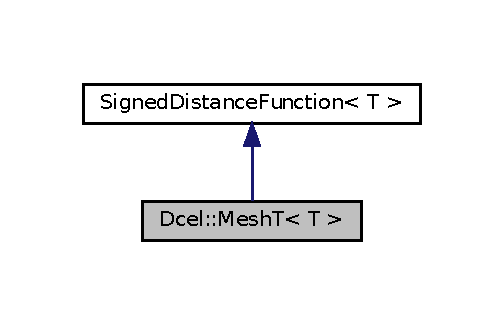
\includegraphics[width=242pt]{classDcel_1_1MeshT__inherit__graph}
\end{center}
\end{figure}


Collaboration diagram for Dcel\+::MeshT$<$ T $>$\+:
\nopagebreak
\begin{figure}[H]
\begin{center}
\leavevmode
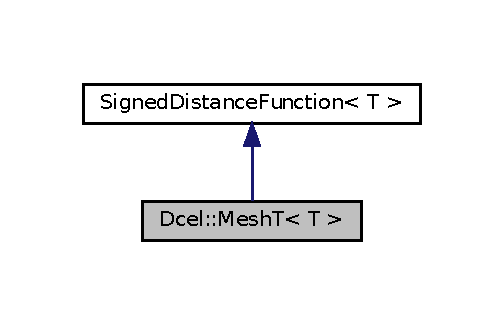
\includegraphics[width=242pt]{classDcel_1_1MeshT__coll__graph}
\end{center}
\end{figure}
\doxysubsection*{Public Types}
\begin{DoxyCompactItemize}
\item 
enum \mbox{\hyperlink{classDcel_1_1MeshT_abb4c3bb7a52804bb041c133f30151399}{Search\+Algorithm}} \{ {\bfseries Direct}, 
{\bfseries Direct2}
 \}
\begin{DoxyCompactList}\small\item\em Possible search algorithms for \mbox{\hyperlink{classDcel_1_1MeshT}{Dcel\+::\+MeshT}}. \end{DoxyCompactList}\item 
\mbox{\Hypertarget{classDcel_1_1MeshT_a0cd3a02853cf4fcc34a0816368ed4dc0}\label{classDcel_1_1MeshT_a0cd3a02853cf4fcc34a0816368ed4dc0}} 
enum \mbox{\hyperlink{classDcel_1_1MeshT_a0cd3a02853cf4fcc34a0816368ed4dc0}{Vertex\+Normal\+Weight}} \{ {\bfseries None}, 
{\bfseries Angle}
 \}
\begin{DoxyCompactList}\small\item\em How to weight vertex normal. \end{DoxyCompactList}\item 
\mbox{\Hypertarget{classDcel_1_1MeshT_a646c5d8f66b3079bca35fe4186493627}\label{classDcel_1_1MeshT_a646c5d8f66b3079bca35fe4186493627}} 
using \mbox{\hyperlink{classDcel_1_1MeshT_a646c5d8f66b3079bca35fe4186493627}{Vec3}} = \mbox{\hyperlink{classVec3T}{Vec3T}}$<$ T $>$
\begin{DoxyCompactList}\small\item\em Alias to cut down on the typing. \end{DoxyCompactList}\item 
\mbox{\Hypertarget{classDcel_1_1MeshT_a58b357c4ad94f4a4b813ed7ebf01cd05}\label{classDcel_1_1MeshT_a58b357c4ad94f4a4b813ed7ebf01cd05}} 
using \mbox{\hyperlink{classDcel_1_1MeshT_a58b357c4ad94f4a4b813ed7ebf01cd05}{Vertex}} = \mbox{\hyperlink{classDcel_1_1VertexT}{VertexT}}$<$ T $>$
\begin{DoxyCompactList}\small\item\em Alias to cut down on the typing. \end{DoxyCompactList}\item 
\mbox{\Hypertarget{classDcel_1_1MeshT_a94f5c42e6f80fd948ebbc294d948ffab}\label{classDcel_1_1MeshT_a94f5c42e6f80fd948ebbc294d948ffab}} 
using \mbox{\hyperlink{classDcel_1_1MeshT_a94f5c42e6f80fd948ebbc294d948ffab}{Edge}} = \mbox{\hyperlink{classDcel_1_1EdgeT}{EdgeT}}$<$ T $>$
\begin{DoxyCompactList}\small\item\em Alias to cut down on the typing. \end{DoxyCompactList}\item 
\mbox{\Hypertarget{classDcel_1_1MeshT_ac1fcce96c65811660619af9eb32589f9}\label{classDcel_1_1MeshT_ac1fcce96c65811660619af9eb32589f9}} 
using \mbox{\hyperlink{classDcel_1_1MeshT_ac1fcce96c65811660619af9eb32589f9}{Face}} = \mbox{\hyperlink{classDcel_1_1FaceT}{FaceT}}$<$ T $>$
\begin{DoxyCompactList}\small\item\em Alias to cut down on the typing. \end{DoxyCompactList}\item 
\mbox{\Hypertarget{classDcel_1_1MeshT_a1e0abeadcb51e679b0dd9a36e2ee08c7}\label{classDcel_1_1MeshT_a1e0abeadcb51e679b0dd9a36e2ee08c7}} 
using \mbox{\hyperlink{classDcel_1_1MeshT_a1e0abeadcb51e679b0dd9a36e2ee08c7}{Vertex\+Ptr}} = std\+::shared\+\_\+ptr$<$ \mbox{\hyperlink{classDcel_1_1MeshT_a58b357c4ad94f4a4b813ed7ebf01cd05}{Vertex}} $>$
\begin{DoxyCompactList}\small\item\em Alias to cut down on the typing. \end{DoxyCompactList}\item 
\mbox{\Hypertarget{classDcel_1_1MeshT_ab2b035530536a8bc56e40aab455f24e3}\label{classDcel_1_1MeshT_ab2b035530536a8bc56e40aab455f24e3}} 
using \mbox{\hyperlink{classDcel_1_1MeshT_ab2b035530536a8bc56e40aab455f24e3}{Edge\+Ptr}} = std\+::shared\+\_\+ptr$<$ \mbox{\hyperlink{classDcel_1_1MeshT_a94f5c42e6f80fd948ebbc294d948ffab}{Edge}} $>$
\begin{DoxyCompactList}\small\item\em Alias to cut down on the typing. \end{DoxyCompactList}\item 
\mbox{\Hypertarget{classDcel_1_1MeshT_a6c71642a9e6b36f9d6ab6027035625f0}\label{classDcel_1_1MeshT_a6c71642a9e6b36f9d6ab6027035625f0}} 
using \mbox{\hyperlink{classDcel_1_1MeshT_a6c71642a9e6b36f9d6ab6027035625f0}{Face\+Ptr}} = std\+::shared\+\_\+ptr$<$ \mbox{\hyperlink{classDcel_1_1MeshT_ac1fcce96c65811660619af9eb32589f9}{Face}} $>$
\begin{DoxyCompactList}\small\item\em Alias to cut down on the typing. \end{DoxyCompactList}\item 
\mbox{\Hypertarget{classDcel_1_1MeshT_abe9db973f4510ccb36e20ecfa9223926}\label{classDcel_1_1MeshT_abe9db973f4510ccb36e20ecfa9223926}} 
using \mbox{\hyperlink{classDcel_1_1MeshT_abe9db973f4510ccb36e20ecfa9223926}{Mesh}} = \mbox{\hyperlink{classDcel_1_1MeshT}{MeshT}}$<$ T $>$
\begin{DoxyCompactList}\small\item\em Alias to cut down on the typing. \end{DoxyCompactList}\end{DoxyCompactItemize}
\doxysubsection*{Public Member Functions}
\begin{DoxyCompactItemize}
\item 
\mbox{\Hypertarget{classDcel_1_1MeshT_a4eae06529761d8aff54e945eb0a3ba91}\label{classDcel_1_1MeshT_a4eae06529761d8aff54e945eb0a3ba91}} 
\mbox{\hyperlink{classDcel_1_1MeshT_a4eae06529761d8aff54e945eb0a3ba91}{MeshT}} ()
\begin{DoxyCompactList}\small\item\em Default constructor. Leaves unobject in an unusable state. \end{DoxyCompactList}\item 
\mbox{\hyperlink{classDcel_1_1MeshT_aa055e10c62778ba629b3f9c849338e03}{MeshT}} (const \mbox{\hyperlink{classDcel_1_1MeshT_abe9db973f4510ccb36e20ecfa9223926}{Mesh}} \&a\+\_\+other\+Mesh)=delete
\begin{DoxyCompactList}\small\item\em Disallowed copy construction. \end{DoxyCompactList}\item 
\mbox{\hyperlink{classDcel_1_1MeshT_a7468e3630893d64a71a7c2347496576b}{MeshT}} (std\+::vector$<$ \mbox{\hyperlink{classDcel_1_1MeshT_a6c71642a9e6b36f9d6ab6027035625f0}{Face\+Ptr}} $>$ \&a\+\_\+faces, std\+::vector$<$ \mbox{\hyperlink{classDcel_1_1MeshT_ab2b035530536a8bc56e40aab455f24e3}{Edge\+Ptr}} $>$ \&a\+\_\+edges, std\+::vector$<$ \mbox{\hyperlink{classDcel_1_1MeshT_a1e0abeadcb51e679b0dd9a36e2ee08c7}{Vertex\+Ptr}} $>$ \&a\+\_\+vertices)
\begin{DoxyCompactList}\small\item\em Full constructor. This provides the faces, edges, and vertices to the mesh. \end{DoxyCompactList}\item 
\mbox{\Hypertarget{classDcel_1_1MeshT_a51da8ad54b3cfe69a695221f73bd97b2}\label{classDcel_1_1MeshT_a51da8ad54b3cfe69a695221f73bd97b2}} 
\mbox{\hyperlink{classDcel_1_1MeshT_a51da8ad54b3cfe69a695221f73bd97b2}{$\sim$\+MeshT}} ()
\begin{DoxyCompactList}\small\item\em Destructor (does nothing) \end{DoxyCompactList}\item 
void \mbox{\hyperlink{classDcel_1_1MeshT_af65f5fc459d586ba3b6bd0711b0951f5}{define}} (std\+::vector$<$ \mbox{\hyperlink{classDcel_1_1MeshT_a6c71642a9e6b36f9d6ab6027035625f0}{Face\+Ptr}} $>$ \&a\+\_\+faces, std\+::vector$<$ \mbox{\hyperlink{classDcel_1_1MeshT_ab2b035530536a8bc56e40aab455f24e3}{Edge\+Ptr}} $>$ \&a\+\_\+edges, std\+::vector$<$ \mbox{\hyperlink{classDcel_1_1MeshT_a1e0abeadcb51e679b0dd9a36e2ee08c7}{Vertex\+Ptr}} $>$ \&a\+\_\+vertices) noexcept
\begin{DoxyCompactList}\small\item\em Define function. Puts Mesh in usable state. \end{DoxyCompactList}\item 
void \mbox{\hyperlink{classDcel_1_1MeshT_a1814ba63c6e0d7a007ee78c24d6ea159}{sanity\+Check}} () const noexcept
\begin{DoxyCompactList}\small\item\em Perform a sanity check. \end{DoxyCompactList}\item 
void \mbox{\hyperlink{classDcel_1_1MeshT_abc7a2bd7632be06c0ad9cf49816d262f}{set\+Search\+Algorithm}} (const \mbox{\hyperlink{classDcel_1_1MeshT_abb4c3bb7a52804bb041c133f30151399}{Search\+Algorithm}} a\+\_\+algorithm) noexcept
\begin{DoxyCompactList}\small\item\em Search algorithm for direct signed distance computations. \end{DoxyCompactList}\item 
void \mbox{\hyperlink{classDcel_1_1MeshT_a1e46a744a2526e451229e2f2e4830ca5}{set\+Inside\+Outside\+Algorithm}} (typename \mbox{\hyperlink{classDcel_1_1Polygon2D}{Dcel\+::\+Polygon2D}}$<$ T $>$\+::Inside\+Outside\+Algorithm a\+\_\+algorithm) noexcept
\begin{DoxyCompactList}\small\item\em Set the inside/outside algorithm to use when computing the signed distance to polygon faces. \end{DoxyCompactList}\item 
void \mbox{\hyperlink{classDcel_1_1MeshT_a98d80b5f83b9d6ff55d0d0da34d0b422}{reconcile}} (typename \mbox{\hyperlink{classDcel_1_1MeshT}{Dcel\+::\+MeshT}}$<$ T $>$\+::\mbox{\hyperlink{classDcel_1_1MeshT_a0cd3a02853cf4fcc34a0816368ed4dc0}{Vertex\+Normal\+Weight}} a\+\_\+weight=Vertex\+Normal\+Weight\+::\+Angle) noexcept
\begin{DoxyCompactList}\small\item\em Reconcile function which computes the internal parameters in vertices, edges, and faces for use with signed distance functionality. \end{DoxyCompactList}\item 
\mbox{\Hypertarget{classDcel_1_1MeshT_af9a71c79cdd18793d20233516974936c}\label{classDcel_1_1MeshT_af9a71c79cdd18793d20233516974936c}} 
std\+::vector$<$ \mbox{\hyperlink{classDcel_1_1MeshT_a1e0abeadcb51e679b0dd9a36e2ee08c7}{Vertex\+Ptr}} $>$ \& \mbox{\hyperlink{classDcel_1_1MeshT_af9a71c79cdd18793d20233516974936c}{get\+Vertices}} () noexcept
\begin{DoxyCompactList}\small\item\em Get modifiable vertices in this mesh. \end{DoxyCompactList}\item 
\mbox{\Hypertarget{classDcel_1_1MeshT_af2ec265fb18c2cc90be227f9e1b3faa1}\label{classDcel_1_1MeshT_af2ec265fb18c2cc90be227f9e1b3faa1}} 
const std\+::vector$<$ \mbox{\hyperlink{classDcel_1_1MeshT_a1e0abeadcb51e679b0dd9a36e2ee08c7}{Vertex\+Ptr}} $>$ \& \mbox{\hyperlink{classDcel_1_1MeshT_af2ec265fb18c2cc90be227f9e1b3faa1}{get\+Vertices}} () const noexcept
\begin{DoxyCompactList}\small\item\em Get immutable vertices in this mesh. \end{DoxyCompactList}\item 
\mbox{\Hypertarget{classDcel_1_1MeshT_a953967f06953cb5c1fdf3d29e108cb36}\label{classDcel_1_1MeshT_a953967f06953cb5c1fdf3d29e108cb36}} 
std\+::vector$<$ \mbox{\hyperlink{classDcel_1_1MeshT_ab2b035530536a8bc56e40aab455f24e3}{Edge\+Ptr}} $>$ \& \mbox{\hyperlink{classDcel_1_1MeshT_a953967f06953cb5c1fdf3d29e108cb36}{get\+Edges}} () noexcept
\begin{DoxyCompactList}\small\item\em Get modifiable half-\/edges in this mesh. \end{DoxyCompactList}\item 
\mbox{\Hypertarget{classDcel_1_1MeshT_a52f24998efeafc66c92c1d30d36d3617}\label{classDcel_1_1MeshT_a52f24998efeafc66c92c1d30d36d3617}} 
const std\+::vector$<$ \mbox{\hyperlink{classDcel_1_1MeshT_ab2b035530536a8bc56e40aab455f24e3}{Edge\+Ptr}} $>$ \& \mbox{\hyperlink{classDcel_1_1MeshT_a52f24998efeafc66c92c1d30d36d3617}{get\+Edges}} () const noexcept
\begin{DoxyCompactList}\small\item\em Get immutable half-\/edges in this mesh. \end{DoxyCompactList}\item 
\mbox{\Hypertarget{classDcel_1_1MeshT_a4e27345d28c3f307df8b759644a6a50b}\label{classDcel_1_1MeshT_a4e27345d28c3f307df8b759644a6a50b}} 
std\+::vector$<$ \mbox{\hyperlink{classDcel_1_1MeshT_a6c71642a9e6b36f9d6ab6027035625f0}{Face\+Ptr}} $>$ \& \mbox{\hyperlink{classDcel_1_1MeshT_a4e27345d28c3f307df8b759644a6a50b}{get\+Faces}} () noexcept
\begin{DoxyCompactList}\small\item\em Get modifiable faces in this mesh. \end{DoxyCompactList}\item 
\mbox{\Hypertarget{classDcel_1_1MeshT_a7f1891fc07bf4f353fb7251723f7fd46}\label{classDcel_1_1MeshT_a7f1891fc07bf4f353fb7251723f7fd46}} 
const std\+::vector$<$ \mbox{\hyperlink{classDcel_1_1MeshT_a6c71642a9e6b36f9d6ab6027035625f0}{Face\+Ptr}} $>$ \& \mbox{\hyperlink{classDcel_1_1MeshT_a7f1891fc07bf4f353fb7251723f7fd46}{get\+Faces}} () const noexcept
\begin{DoxyCompactList}\small\item\em Get immutable faces in this mesh. \end{DoxyCompactList}\item 
T \mbox{\hyperlink{classDcel_1_1MeshT_a0e16e8fcf1a73342c87c35e3b5682dae}{signed\+Distance}} (const \mbox{\hyperlink{classDcel_1_1MeshT_a646c5d8f66b3079bca35fe4186493627}{Vec3}} \&a\+\_\+x0) const noexcept override
\begin{DoxyCompactList}\small\item\em Compute the signed distance from a point to this mesh. \end{DoxyCompactList}\item 
T \mbox{\hyperlink{classDcel_1_1MeshT_a4fa40378fbd4c31cd50e77da70ef30fd}{signed\+Distance}} (const \mbox{\hyperlink{classDcel_1_1MeshT_a646c5d8f66b3079bca35fe4186493627}{Vec3}} \&a\+\_\+x0, \mbox{\hyperlink{classDcel_1_1MeshT_abb4c3bb7a52804bb041c133f30151399}{Search\+Algorithm}} a\+\_\+algorithm) const noexcept
\begin{DoxyCompactList}\small\item\em Compute the signed distance from a point to this mesh. \end{DoxyCompactList}\item 
T \mbox{\hyperlink{classDcel_1_1MeshT_a8be4c3d6f606b8bc8cc36820de773de1}{unsigned\+Distance2}} (const \mbox{\hyperlink{classDcel_1_1MeshT_a646c5d8f66b3079bca35fe4186493627}{Vec3}} \&a\+\_\+x0) const noexcept
\begin{DoxyCompactList}\small\item\em Compute the unsigned square distance from a point to this mesh. \end{DoxyCompactList}\end{DoxyCompactItemize}
\doxysubsection*{Protected Member Functions}
\begin{DoxyCompactItemize}
\item 
\mbox{\Hypertarget{classDcel_1_1MeshT_a597a38ed9f3e3a2a33f2d1211da322f3}\label{classDcel_1_1MeshT_a597a38ed9f3e3a2a33f2d1211da322f3}} 
std\+::vector$<$ \mbox{\hyperlink{classVec3T}{Vec3T}}$<$ T $>$ $>$ \mbox{\hyperlink{classDcel_1_1MeshT_a597a38ed9f3e3a2a33f2d1211da322f3}{get\+All\+Vertex\+Coordinates}} () const noexcept
\begin{DoxyCompactList}\small\item\em Return all vertex coordinates in the mesh. \end{DoxyCompactList}\item 
void \mbox{\hyperlink{classDcel_1_1MeshT_a5e31ae8b95c9ee725e205d8ae4fd35dc}{reconcile\+Faces}} () noexcept
\begin{DoxyCompactList}\small\item\em Function which computes internal things for the polygon faces. \end{DoxyCompactList}\item 
void \mbox{\hyperlink{classDcel_1_1MeshT_a33f6506c1daf9946d1f21117c0ab89d5}{reconcile\+Edges}} () noexcept
\begin{DoxyCompactList}\small\item\em Function which computes internal things for the half-\/edges. \end{DoxyCompactList}\item 
void \mbox{\hyperlink{classDcel_1_1MeshT_ad2b65aa214d51ecd438bc876e7255290}{reconcile\+Vertices}} (typename \mbox{\hyperlink{classDcel_1_1MeshT}{Dcel\+::\+MeshT}}$<$ T $>$\+::\mbox{\hyperlink{classDcel_1_1MeshT_a0cd3a02853cf4fcc34a0816368ed4dc0}{Vertex\+Normal\+Weight}} a\+\_\+weight) noexcept
\begin{DoxyCompactList}\small\item\em Function which computes internal things for the vertices. \end{DoxyCompactList}\item 
T \mbox{\hyperlink{classDcel_1_1MeshT_ada074ff3b1a612e46098f4ba6ca0bda2}{Direct\+Signed\+Distance}} (const \mbox{\hyperlink{classDcel_1_1MeshT_a646c5d8f66b3079bca35fe4186493627}{Vec3}} \&a\+\_\+point) const noexcept
\begin{DoxyCompactList}\small\item\em Implementation of signed distance function which iterates through all faces. \end{DoxyCompactList}\item 
T \mbox{\hyperlink{classDcel_1_1MeshT_ac00a6da46649246a3a2db70b29bb2407}{Direct\+Signed\+Distance2}} (const \mbox{\hyperlink{classDcel_1_1MeshT_a646c5d8f66b3079bca35fe4186493627}{Vec3}} \&a\+\_\+point) const noexcept
\begin{DoxyCompactList}\small\item\em Implementation of squared signed distance function which iterates through all faces. \end{DoxyCompactList}\item 
void \mbox{\hyperlink{classDcel_1_1MeshT_ae13801eefa60ad08ff1da0df1da34784}{increment\+Warning}} (std\+::map$<$ std\+::string, int $>$ \&a\+\_\+warnings, const std\+::string \&a\+\_\+warn) const noexcept
\begin{DoxyCompactList}\small\item\em Increment a warning. This is used in \mbox{\hyperlink{classDcel_1_1MeshT_a1814ba63c6e0d7a007ee78c24d6ea159}{sanity\+Check()}} for locating holes or bad inputs in the mesh. \end{DoxyCompactList}\item 
\mbox{\Hypertarget{classDcel_1_1MeshT_a7115bea1b9d776a5f9c82a1e4fe852a0}\label{classDcel_1_1MeshT_a7115bea1b9d776a5f9c82a1e4fe852a0}} 
void \mbox{\hyperlink{classDcel_1_1MeshT_a7115bea1b9d776a5f9c82a1e4fe852a0}{print\+Warnings}} (const std\+::map$<$ std\+::string, int $>$ \&a\+\_\+warnings) const noexcept
\begin{DoxyCompactList}\small\item\em Print all warnings to std\+::cerr. \end{DoxyCompactList}\end{DoxyCompactItemize}
\doxysubsection*{Protected Attributes}
\begin{DoxyCompactItemize}
\item 
\mbox{\Hypertarget{classDcel_1_1MeshT_aaa5bdf8df02aa8bcff84203467f86fbe}\label{classDcel_1_1MeshT_aaa5bdf8df02aa8bcff84203467f86fbe}} 
\mbox{\hyperlink{classDcel_1_1MeshT_abb4c3bb7a52804bb041c133f30151399}{Search\+Algorithm}} \mbox{\hyperlink{classDcel_1_1MeshT_aaa5bdf8df02aa8bcff84203467f86fbe}{m\+\_\+algorithm}}
\begin{DoxyCompactList}\small\item\em Search algorithm. Only used in signed distance functions. \end{DoxyCompactList}\item 
\mbox{\Hypertarget{classDcel_1_1MeshT_a4263fd9ebba22b96e12ee9f046eca089}\label{classDcel_1_1MeshT_a4263fd9ebba22b96e12ee9f046eca089}} 
std\+::vector$<$ \mbox{\hyperlink{classDcel_1_1MeshT_a1e0abeadcb51e679b0dd9a36e2ee08c7}{Vertex\+Ptr}} $>$ \mbox{\hyperlink{classDcel_1_1MeshT_a4263fd9ebba22b96e12ee9f046eca089}{m\+\_\+vertices}}
\begin{DoxyCompactList}\small\item\em Mesh vertices. \end{DoxyCompactList}\item 
\mbox{\Hypertarget{classDcel_1_1MeshT_a3325cb09037fa32255aa1a8a5536e473}\label{classDcel_1_1MeshT_a3325cb09037fa32255aa1a8a5536e473}} 
std\+::vector$<$ \mbox{\hyperlink{classDcel_1_1MeshT_ab2b035530536a8bc56e40aab455f24e3}{Edge\+Ptr}} $>$ \mbox{\hyperlink{classDcel_1_1MeshT_a3325cb09037fa32255aa1a8a5536e473}{m\+\_\+edges}}
\begin{DoxyCompactList}\small\item\em Mesh half-\/edges. \end{DoxyCompactList}\item 
\mbox{\Hypertarget{classDcel_1_1MeshT_a17e08b2ee4b5b7b1dc3df974e792ca5f}\label{classDcel_1_1MeshT_a17e08b2ee4b5b7b1dc3df974e792ca5f}} 
std\+::vector$<$ \mbox{\hyperlink{classDcel_1_1MeshT_a6c71642a9e6b36f9d6ab6027035625f0}{Face\+Ptr}} $>$ \mbox{\hyperlink{classDcel_1_1MeshT_a17e08b2ee4b5b7b1dc3df974e792ca5f}{m\+\_\+faces}}
\begin{DoxyCompactList}\small\item\em Mesh faces. \end{DoxyCompactList}\end{DoxyCompactItemize}


\doxysubsection{Detailed Description}
\subsubsection*{template$<$class T$>$\newline
class Dcel\+::\+Mesh\+T$<$ T $>$}

Mesh class which stores a full D\+C\+EL mesh (with signed distance functions) 

This encapsulates a full D\+C\+EL mesh, and also includes D\+I\+R\+E\+CT signed distance functions. The mesh consists of a set of vertices, half-\/edges, and polygon faces who each have references to other vertices, half-\/edges, and polygon faces. The signed distance functions D\+I\+R\+E\+CT, which means that they go through A\+LL of the polygon faces and compute the signed distance to them. This is extremely inefficient, which is why this class is almost always embedded into a bounding volume hierarchy. \begin{DoxyNote}{Note}
This class is not for the light of heart -- it will almost always be instantiated through a file parser which reads vertices and edges from file and builds the mesh from that. Do not try to build a \mbox{\hyperlink{classDcel_1_1MeshT}{MeshT}} object yourself, use file parsers! 
\end{DoxyNote}


\doxysubsection{Member Enumeration Documentation}
\mbox{\Hypertarget{classDcel_1_1MeshT_abb4c3bb7a52804bb041c133f30151399}\label{classDcel_1_1MeshT_abb4c3bb7a52804bb041c133f30151399}} 
\index{Dcel::MeshT$<$ T $>$@{Dcel::MeshT$<$ T $>$}!SearchAlgorithm@{SearchAlgorithm}}
\index{SearchAlgorithm@{SearchAlgorithm}!Dcel::MeshT$<$ T $>$@{Dcel::MeshT$<$ T $>$}}
\doxysubsubsection{\texorpdfstring{SearchAlgorithm}{SearchAlgorithm}}
{\footnotesize\ttfamily template$<$class T $>$ \\
enum \mbox{\hyperlink{classDcel_1_1MeshT_abb4c3bb7a52804bb041c133f30151399}{Dcel\+::\+Mesh\+T\+::\+Search\+Algorithm}}\hspace{0.3cm}{\ttfamily [strong]}}



Possible search algorithms for \mbox{\hyperlink{classDcel_1_1MeshT}{Dcel\+::\+MeshT}}. 

Direct means compute the signed distance for all primitives, Direct2 means compute the squared signed distance for all primitives. 

\doxysubsection{Constructor \& Destructor Documentation}
\mbox{\Hypertarget{classDcel_1_1MeshT_aa055e10c62778ba629b3f9c849338e03}\label{classDcel_1_1MeshT_aa055e10c62778ba629b3f9c849338e03}} 
\index{Dcel::MeshT$<$ T $>$@{Dcel::MeshT$<$ T $>$}!MeshT@{MeshT}}
\index{MeshT@{MeshT}!Dcel::MeshT$<$ T $>$@{Dcel::MeshT$<$ T $>$}}
\doxysubsubsection{\texorpdfstring{MeshT()}{MeshT()}\hspace{0.1cm}{\footnotesize\ttfamily [1/2]}}
{\footnotesize\ttfamily template$<$class T $>$ \\
\mbox{\hyperlink{classDcel_1_1MeshT}{Dcel\+::\+MeshT}}$<$ T $>$\+::\mbox{\hyperlink{classDcel_1_1MeshT}{MeshT}} (\begin{DoxyParamCaption}\item[{const \mbox{\hyperlink{classDcel_1_1MeshT_abe9db973f4510ccb36e20ecfa9223926}{Mesh}} \&}]{a\+\_\+other\+Mesh }\end{DoxyParamCaption})\hspace{0.3cm}{\ttfamily [delete]}}



Disallowed copy construction. 


\begin{DoxyParams}[1]{Parameters}
\mbox{\texttt{ in}}  & {\em a\+\_\+other\+Mesh} & Other mesh \\
\hline
\end{DoxyParams}
\mbox{\Hypertarget{classDcel_1_1MeshT_a7468e3630893d64a71a7c2347496576b}\label{classDcel_1_1MeshT_a7468e3630893d64a71a7c2347496576b}} 
\index{Dcel::MeshT$<$ T $>$@{Dcel::MeshT$<$ T $>$}!MeshT@{MeshT}}
\index{MeshT@{MeshT}!Dcel::MeshT$<$ T $>$@{Dcel::MeshT$<$ T $>$}}
\doxysubsubsection{\texorpdfstring{MeshT()}{MeshT()}\hspace{0.1cm}{\footnotesize\ttfamily [2/2]}}
{\footnotesize\ttfamily template$<$class T $>$ \\
\mbox{\hyperlink{classDcel_1_1MeshT}{Dcel\+::\+MeshT}}$<$ T $>$\+::\mbox{\hyperlink{classDcel_1_1MeshT}{MeshT}} (\begin{DoxyParamCaption}\item[{std\+::vector$<$ \mbox{\hyperlink{classDcel_1_1MeshT_a6c71642a9e6b36f9d6ab6027035625f0}{Face\+Ptr}} $>$ \&}]{a\+\_\+faces,  }\item[{std\+::vector$<$ \mbox{\hyperlink{classDcel_1_1MeshT_ab2b035530536a8bc56e40aab455f24e3}{Edge\+Ptr}} $>$ \&}]{a\+\_\+edges,  }\item[{std\+::vector$<$ \mbox{\hyperlink{classDcel_1_1MeshT_a1e0abeadcb51e679b0dd9a36e2ee08c7}{Vertex\+Ptr}} $>$ \&}]{a\+\_\+vertices }\end{DoxyParamCaption})\hspace{0.3cm}{\ttfamily [inline]}}



Full constructor. This provides the faces, edges, and vertices to the mesh. 

Calls define(a\+\_\+faces, a\+\_\+edges, a\+\_\+vertices) 
\begin{DoxyParams}[1]{Parameters}
\mbox{\texttt{ in}}  & {\em a\+\_\+faces} & Polygon faces \\
\hline
\mbox{\texttt{ in}}  & {\em a\+\_\+edges} & Half-\/edges \\
\hline
\mbox{\texttt{ in}}  & {\em a\+\_\+vertices} & Vertices \\
\hline
\end{DoxyParams}
\begin{DoxyNote}{Note}
The constructor arguments should provide a complete D\+C\+EL mesh description. This is usually done through a file parser which reads a mesh file format and creates the D\+C\+EL mesh structure 
\end{DoxyNote}


\doxysubsection{Member Function Documentation}
\mbox{\Hypertarget{classDcel_1_1MeshT_af65f5fc459d586ba3b6bd0711b0951f5}\label{classDcel_1_1MeshT_af65f5fc459d586ba3b6bd0711b0951f5}} 
\index{Dcel::MeshT$<$ T $>$@{Dcel::MeshT$<$ T $>$}!define@{define}}
\index{define@{define}!Dcel::MeshT$<$ T $>$@{Dcel::MeshT$<$ T $>$}}
\doxysubsubsection{\texorpdfstring{define()}{define()}}
{\footnotesize\ttfamily template$<$class T $>$ \\
void \mbox{\hyperlink{classDcel_1_1MeshT}{Dcel\+::\+MeshT}}$<$ T $>$\+::define (\begin{DoxyParamCaption}\item[{std\+::vector$<$ \mbox{\hyperlink{classDcel_1_1MeshT_a6c71642a9e6b36f9d6ab6027035625f0}{Face\+Ptr}} $>$ \&}]{a\+\_\+faces,  }\item[{std\+::vector$<$ \mbox{\hyperlink{classDcel_1_1MeshT_ab2b035530536a8bc56e40aab455f24e3}{Edge\+Ptr}} $>$ \&}]{a\+\_\+edges,  }\item[{std\+::vector$<$ \mbox{\hyperlink{classDcel_1_1MeshT_a1e0abeadcb51e679b0dd9a36e2ee08c7}{Vertex\+Ptr}} $>$ \&}]{a\+\_\+vertices }\end{DoxyParamCaption})\hspace{0.3cm}{\ttfamily [inline]}, {\ttfamily [noexcept]}}



Define function. Puts Mesh in usable state. 


\begin{DoxyParams}[1]{Parameters}
\mbox{\texttt{ in}}  & {\em a\+\_\+faces} & Polygon faces \\
\hline
\mbox{\texttt{ in}}  & {\em a\+\_\+edges} & Half-\/edges \\
\hline
\mbox{\texttt{ in}}  & {\em a\+\_\+vertices} & Vertices \\
\hline
\end{DoxyParams}
\begin{DoxyNote}{Note}
The function arguments should provide a complete D\+C\+EL mesh description. This is usually done through a file parser which reads a mesh file format and creates the D\+C\+EL mesh structure. Note that this only involves associating pointer structures through the mesh. Internal parameters like face area and normal is computed in \mbox{\hyperlink{classDcel_1_1MeshT_a98d80b5f83b9d6ff55d0d0da34d0b422}{Mesh\+T$<$\+T$>$\+::reconcile}}. 
\end{DoxyNote}
\mbox{\Hypertarget{classDcel_1_1MeshT_ada074ff3b1a612e46098f4ba6ca0bda2}\label{classDcel_1_1MeshT_ada074ff3b1a612e46098f4ba6ca0bda2}} 
\index{Dcel::MeshT$<$ T $>$@{Dcel::MeshT$<$ T $>$}!DirectSignedDistance@{DirectSignedDistance}}
\index{DirectSignedDistance@{DirectSignedDistance}!Dcel::MeshT$<$ T $>$@{Dcel::MeshT$<$ T $>$}}
\doxysubsubsection{\texorpdfstring{DirectSignedDistance()}{DirectSignedDistance()}}
{\footnotesize\ttfamily template$<$class T $>$ \\
T \mbox{\hyperlink{classDcel_1_1MeshT}{Dcel\+::\+MeshT}}$<$ T $>$\+::Direct\+Signed\+Distance (\begin{DoxyParamCaption}\item[{const \mbox{\hyperlink{classDcel_1_1MeshT_a646c5d8f66b3079bca35fe4186493627}{Vec3}} \&}]{a\+\_\+point }\end{DoxyParamCaption}) const\hspace{0.3cm}{\ttfamily [inline]}, {\ttfamily [protected]}, {\ttfamily [noexcept]}}



Implementation of signed distance function which iterates through all faces. 


\begin{DoxyParams}[1]{Parameters}
\mbox{\texttt{ in}}  & {\em a\+\_\+point} & 3D point \\
\hline
\end{DoxyParams}
\mbox{\Hypertarget{classDcel_1_1MeshT_ac00a6da46649246a3a2db70b29bb2407}\label{classDcel_1_1MeshT_ac00a6da46649246a3a2db70b29bb2407}} 
\index{Dcel::MeshT$<$ T $>$@{Dcel::MeshT$<$ T $>$}!DirectSignedDistance2@{DirectSignedDistance2}}
\index{DirectSignedDistance2@{DirectSignedDistance2}!Dcel::MeshT$<$ T $>$@{Dcel::MeshT$<$ T $>$}}
\doxysubsubsection{\texorpdfstring{DirectSignedDistance2()}{DirectSignedDistance2()}}
{\footnotesize\ttfamily template$<$class T $>$ \\
T \mbox{\hyperlink{classDcel_1_1MeshT}{Dcel\+::\+MeshT}}$<$ T $>$\+::Direct\+Signed\+Distance2 (\begin{DoxyParamCaption}\item[{const \mbox{\hyperlink{classDcel_1_1MeshT_a646c5d8f66b3079bca35fe4186493627}{Vec3}} \&}]{a\+\_\+point }\end{DoxyParamCaption}) const\hspace{0.3cm}{\ttfamily [inline]}, {\ttfamily [protected]}, {\ttfamily [noexcept]}}



Implementation of squared signed distance function which iterates through all faces. 

This first find the face with the smallest unsigned square distance, and the returns the signed distance to that face (more efficient than the other version). 
\begin{DoxyParams}[1]{Parameters}
\mbox{\texttt{ in}}  & {\em a\+\_\+point} & 3D point \\
\hline
\end{DoxyParams}
\mbox{\Hypertarget{classDcel_1_1MeshT_ae13801eefa60ad08ff1da0df1da34784}\label{classDcel_1_1MeshT_ae13801eefa60ad08ff1da0df1da34784}} 
\index{Dcel::MeshT$<$ T $>$@{Dcel::MeshT$<$ T $>$}!incrementWarning@{incrementWarning}}
\index{incrementWarning@{incrementWarning}!Dcel::MeshT$<$ T $>$@{Dcel::MeshT$<$ T $>$}}
\doxysubsubsection{\texorpdfstring{incrementWarning()}{incrementWarning()}}
{\footnotesize\ttfamily template$<$class T $>$ \\
void \mbox{\hyperlink{classDcel_1_1MeshT}{Dcel\+::\+MeshT}}$<$ T $>$\+::increment\+Warning (\begin{DoxyParamCaption}\item[{std\+::map$<$ std\+::string, int $>$ \&}]{a\+\_\+warnings,  }\item[{const std\+::string \&}]{a\+\_\+warn }\end{DoxyParamCaption}) const\hspace{0.3cm}{\ttfamily [inline]}, {\ttfamily [protected]}, {\ttfamily [noexcept]}}



Increment a warning. This is used in \mbox{\hyperlink{classDcel_1_1MeshT_a1814ba63c6e0d7a007ee78c24d6ea159}{sanity\+Check()}} for locating holes or bad inputs in the mesh. 


\begin{DoxyParams}[1]{Parameters}
\mbox{\texttt{ in}}  & {\em a\+\_\+warnings} & Map of all registered warnings \\
\hline
\mbox{\texttt{ in}}  & {\em a\+\_\+warn} & Current warning to increment by \\
\hline
\end{DoxyParams}
\mbox{\Hypertarget{classDcel_1_1MeshT_a98d80b5f83b9d6ff55d0d0da34d0b422}\label{classDcel_1_1MeshT_a98d80b5f83b9d6ff55d0d0da34d0b422}} 
\index{Dcel::MeshT$<$ T $>$@{Dcel::MeshT$<$ T $>$}!reconcile@{reconcile}}
\index{reconcile@{reconcile}!Dcel::MeshT$<$ T $>$@{Dcel::MeshT$<$ T $>$}}
\doxysubsubsection{\texorpdfstring{reconcile()}{reconcile()}}
{\footnotesize\ttfamily template$<$class T $>$ \\
void \mbox{\hyperlink{classDcel_1_1MeshT}{Dcel\+::\+MeshT}}$<$ T $>$\+::reconcile (\begin{DoxyParamCaption}\item[{typename \mbox{\hyperlink{classDcel_1_1MeshT}{Dcel\+::\+MeshT}}$<$ T $>$\+::\mbox{\hyperlink{classDcel_1_1MeshT_a0cd3a02853cf4fcc34a0816368ed4dc0}{Vertex\+Normal\+Weight}}}]{a\+\_\+weight = {\ttfamily VertexNormalWeight\+:\+:Angle} }\end{DoxyParamCaption})\hspace{0.3cm}{\ttfamily [inline]}, {\ttfamily [noexcept]}}



Reconcile function which computes the internal parameters in vertices, edges, and faces for use with signed distance functionality. 


\begin{DoxyParams}[1]{Parameters}
\mbox{\texttt{ in}}  & {\em a\+\_\+weight} & Vertex angle weighting function. Either Vertex\+Normal\+Weight\+::\+None for unweighted vertex normals or Vertex\+Normal\+Weight\+::\+Angle for the pseudonormal\\
\hline
\end{DoxyParams}
This will reconcile faces, edges, and vertices, e.\+g. computing the area and normal vector for faces \mbox{\Hypertarget{classDcel_1_1MeshT_a33f6506c1daf9946d1f21117c0ab89d5}\label{classDcel_1_1MeshT_a33f6506c1daf9946d1f21117c0ab89d5}} 
\index{Dcel::MeshT$<$ T $>$@{Dcel::MeshT$<$ T $>$}!reconcileEdges@{reconcileEdges}}
\index{reconcileEdges@{reconcileEdges}!Dcel::MeshT$<$ T $>$@{Dcel::MeshT$<$ T $>$}}
\doxysubsubsection{\texorpdfstring{reconcileEdges()}{reconcileEdges()}}
{\footnotesize\ttfamily template$<$class T $>$ \\
void \mbox{\hyperlink{classDcel_1_1MeshT}{Dcel\+::\+MeshT}}$<$ T $>$\+::reconcile\+Edges\hspace{0.3cm}{\ttfamily [inline]}, {\ttfamily [protected]}, {\ttfamily [noexcept]}}



Function which computes internal things for the half-\/edges. 

\begin{DoxyNote}{Note}
This calls \mbox{\hyperlink{classDcel_1_1EdgeT_ac4aaf294fd41c84ef2f7f54a8024e6dd}{Dcel\+::\+Edge\+T$<$\+T$>$\+::reconcile()}} 
\end{DoxyNote}
\mbox{\Hypertarget{classDcel_1_1MeshT_a5e31ae8b95c9ee725e205d8ae4fd35dc}\label{classDcel_1_1MeshT_a5e31ae8b95c9ee725e205d8ae4fd35dc}} 
\index{Dcel::MeshT$<$ T $>$@{Dcel::MeshT$<$ T $>$}!reconcileFaces@{reconcileFaces}}
\index{reconcileFaces@{reconcileFaces}!Dcel::MeshT$<$ T $>$@{Dcel::MeshT$<$ T $>$}}
\doxysubsubsection{\texorpdfstring{reconcileFaces()}{reconcileFaces()}}
{\footnotesize\ttfamily template$<$class T $>$ \\
void \mbox{\hyperlink{classDcel_1_1MeshT}{Dcel\+::\+MeshT}}$<$ T $>$\+::reconcile\+Faces\hspace{0.3cm}{\ttfamily [inline]}, {\ttfamily [protected]}, {\ttfamily [noexcept]}}



Function which computes internal things for the polygon faces. 

\begin{DoxyNote}{Note}
This calls \mbox{\hyperlink{classDcel_1_1FaceT_aaf3f8b92ca4393391ea213b0ecfe19bd}{Dcel\+::\+Face\+T$<$\+T$>$\+::reconcile()}} 
\end{DoxyNote}
\mbox{\Hypertarget{classDcel_1_1MeshT_ad2b65aa214d51ecd438bc876e7255290}\label{classDcel_1_1MeshT_ad2b65aa214d51ecd438bc876e7255290}} 
\index{Dcel::MeshT$<$ T $>$@{Dcel::MeshT$<$ T $>$}!reconcileVertices@{reconcileVertices}}
\index{reconcileVertices@{reconcileVertices}!Dcel::MeshT$<$ T $>$@{Dcel::MeshT$<$ T $>$}}
\doxysubsubsection{\texorpdfstring{reconcileVertices()}{reconcileVertices()}}
{\footnotesize\ttfamily template$<$class T $>$ \\
void \mbox{\hyperlink{classDcel_1_1MeshT}{Dcel\+::\+MeshT}}$<$ T $>$\+::reconcile\+Vertices (\begin{DoxyParamCaption}\item[{typename \mbox{\hyperlink{classDcel_1_1MeshT}{Dcel\+::\+MeshT}}$<$ T $>$\+::\mbox{\hyperlink{classDcel_1_1MeshT_a0cd3a02853cf4fcc34a0816368ed4dc0}{Vertex\+Normal\+Weight}}}]{a\+\_\+weight }\end{DoxyParamCaption})\hspace{0.3cm}{\ttfamily [inline]}, {\ttfamily [protected]}, {\ttfamily [noexcept]}}



Function which computes internal things for the vertices. 


\begin{DoxyParams}[1]{Parameters}
\mbox{\texttt{ in}}  & {\em a\+\_\+weight} & Vertex angle weighting \\
\hline
\end{DoxyParams}
\begin{DoxyNote}{Note}
This calls \mbox{\hyperlink{classDcel_1_1VertexT_adb439515e1814e3fdd9d040b9c1b22df}{Dcel\+::\+Vertex\+T$<$\+T$>$\+::compute\+Vertex\+Normal\+Average()}} or \mbox{\hyperlink{classDcel_1_1VertexT_aa9e66780ec134afe94d9e5a8221fdc0e}{Dcel\+::\+Vertex\+T$<$\+T$>$\+::compute\+Vertex\+Normal\+Angle\+Weighted()}} 
\end{DoxyNote}
\mbox{\Hypertarget{classDcel_1_1MeshT_a1814ba63c6e0d7a007ee78c24d6ea159}\label{classDcel_1_1MeshT_a1814ba63c6e0d7a007ee78c24d6ea159}} 
\index{Dcel::MeshT$<$ T $>$@{Dcel::MeshT$<$ T $>$}!sanityCheck@{sanityCheck}}
\index{sanityCheck@{sanityCheck}!Dcel::MeshT$<$ T $>$@{Dcel::MeshT$<$ T $>$}}
\doxysubsubsection{\texorpdfstring{sanityCheck()}{sanityCheck()}}
{\footnotesize\ttfamily template$<$class T $>$ \\
void \mbox{\hyperlink{classDcel_1_1MeshT}{Dcel\+::\+MeshT}}$<$ T $>$\+::sanity\+Check\hspace{0.3cm}{\ttfamily [inline]}, {\ttfamily [noexcept]}}



Perform a sanity check. 

This will provide error messages if vertices are badly linked, faces are nullptr, and so on. These messages are logged by calling \mbox{\hyperlink{classDcel_1_1MeshT_ae13801eefa60ad08ff1da0df1da34784}{increment\+Warning()}} which identifies types of errors that can occur, and how many of those errors have occured. \mbox{\Hypertarget{classDcel_1_1MeshT_a1e46a744a2526e451229e2f2e4830ca5}\label{classDcel_1_1MeshT_a1e46a744a2526e451229e2f2e4830ca5}} 
\index{Dcel::MeshT$<$ T $>$@{Dcel::MeshT$<$ T $>$}!setInsideOutsideAlgorithm@{setInsideOutsideAlgorithm}}
\index{setInsideOutsideAlgorithm@{setInsideOutsideAlgorithm}!Dcel::MeshT$<$ T $>$@{Dcel::MeshT$<$ T $>$}}
\doxysubsubsection{\texorpdfstring{setInsideOutsideAlgorithm()}{setInsideOutsideAlgorithm()}}
{\footnotesize\ttfamily template$<$class T $>$ \\
void \mbox{\hyperlink{classDcel_1_1MeshT}{Dcel\+::\+MeshT}}$<$ T $>$\+::set\+Inside\+Outside\+Algorithm (\begin{DoxyParamCaption}\item[{typename \mbox{\hyperlink{classDcel_1_1Polygon2D}{Dcel\+::\+Polygon2D}}$<$ T $>$\+::Inside\+Outside\+Algorithm}]{a\+\_\+algorithm }\end{DoxyParamCaption})\hspace{0.3cm}{\ttfamily [inline]}, {\ttfamily [noexcept]}}



Set the inside/outside algorithm to use when computing the signed distance to polygon faces. 

Computing the signed distance to faces requires testing if a point projected to a polygo face plane falls inside or outside the polygon face. There are multiple algorithms to use here. 
\begin{DoxyParams}[1]{Parameters}
\mbox{\texttt{ in}}  & {\em a\+\_\+algorithm} & Algorithm to use \\
\hline
\end{DoxyParams}
\mbox{\Hypertarget{classDcel_1_1MeshT_abc7a2bd7632be06c0ad9cf49816d262f}\label{classDcel_1_1MeshT_abc7a2bd7632be06c0ad9cf49816d262f}} 
\index{Dcel::MeshT$<$ T $>$@{Dcel::MeshT$<$ T $>$}!setSearchAlgorithm@{setSearchAlgorithm}}
\index{setSearchAlgorithm@{setSearchAlgorithm}!Dcel::MeshT$<$ T $>$@{Dcel::MeshT$<$ T $>$}}
\doxysubsubsection{\texorpdfstring{setSearchAlgorithm()}{setSearchAlgorithm()}}
{\footnotesize\ttfamily template$<$class T $>$ \\
void \mbox{\hyperlink{classDcel_1_1MeshT}{Dcel\+::\+MeshT}}$<$ T $>$\+::set\+Search\+Algorithm (\begin{DoxyParamCaption}\item[{const \mbox{\hyperlink{classDcel_1_1MeshT_abb4c3bb7a52804bb041c133f30151399}{Search\+Algorithm}}}]{a\+\_\+algorithm }\end{DoxyParamCaption})\hspace{0.3cm}{\ttfamily [inline]}, {\ttfamily [noexcept]}}



Search algorithm for direct signed distance computations. 


\begin{DoxyParams}[1]{Parameters}
\mbox{\texttt{ in}}  & {\em a\+\_\+algorithm} & Algorithm to use \\
\hline
\end{DoxyParams}
\mbox{\Hypertarget{classDcel_1_1MeshT_a0e16e8fcf1a73342c87c35e3b5682dae}\label{classDcel_1_1MeshT_a0e16e8fcf1a73342c87c35e3b5682dae}} 
\index{Dcel::MeshT$<$ T $>$@{Dcel::MeshT$<$ T $>$}!signedDistance@{signedDistance}}
\index{signedDistance@{signedDistance}!Dcel::MeshT$<$ T $>$@{Dcel::MeshT$<$ T $>$}}
\doxysubsubsection{\texorpdfstring{signedDistance()}{signedDistance()}\hspace{0.1cm}{\footnotesize\ttfamily [1/2]}}
{\footnotesize\ttfamily template$<$class T $>$ \\
T \mbox{\hyperlink{classDcel_1_1MeshT}{Dcel\+::\+MeshT}}$<$ T $>$\+::signed\+Distance (\begin{DoxyParamCaption}\item[{const \mbox{\hyperlink{classDcel_1_1MeshT_a646c5d8f66b3079bca35fe4186493627}{Vec3}} \&}]{a\+\_\+x0 }\end{DoxyParamCaption}) const\hspace{0.3cm}{\ttfamily [inline]}, {\ttfamily [override]}, {\ttfamily [virtual]}, {\ttfamily [noexcept]}}



Compute the signed distance from a point to this mesh. 


\begin{DoxyParams}[1]{Parameters}
\mbox{\texttt{ in}}  & {\em a\+\_\+x0} & 3D point in space.\\
\hline
\end{DoxyParams}
This function will iterate through A\+LL faces in the mesh and return the value with the smallest magnitude. This is horrendously slow, which is why this function is almost never called. Rather, Mesh\+T$<$\+T$>$ can be embedded in a bounding volume hierarchy for faster access. \begin{DoxyNote}{Note}
This will call the other version with the object\textquotesingle{}s search algorithm. 
\end{DoxyNote}


Implements \mbox{\hyperlink{classSignedDistanceFunction_af5912280ca51dc21a2d6949a30ec7d21}{Signed\+Distance\+Function$<$ T $>$}}.

\mbox{\Hypertarget{classDcel_1_1MeshT_a4fa40378fbd4c31cd50e77da70ef30fd}\label{classDcel_1_1MeshT_a4fa40378fbd4c31cd50e77da70ef30fd}} 
\index{Dcel::MeshT$<$ T $>$@{Dcel::MeshT$<$ T $>$}!signedDistance@{signedDistance}}
\index{signedDistance@{signedDistance}!Dcel::MeshT$<$ T $>$@{Dcel::MeshT$<$ T $>$}}
\doxysubsubsection{\texorpdfstring{signedDistance()}{signedDistance()}\hspace{0.1cm}{\footnotesize\ttfamily [2/2]}}
{\footnotesize\ttfamily template$<$class T $>$ \\
T \mbox{\hyperlink{classDcel_1_1MeshT}{Dcel\+::\+MeshT}}$<$ T $>$\+::signed\+Distance (\begin{DoxyParamCaption}\item[{const \mbox{\hyperlink{classDcel_1_1MeshT_a646c5d8f66b3079bca35fe4186493627}{Vec3}} \&}]{a\+\_\+x0,  }\item[{\mbox{\hyperlink{classDcel_1_1MeshT_abb4c3bb7a52804bb041c133f30151399}{Search\+Algorithm}}}]{a\+\_\+algorithm }\end{DoxyParamCaption}) const\hspace{0.3cm}{\ttfamily [inline]}, {\ttfamily [noexcept]}}



Compute the signed distance from a point to this mesh. 


\begin{DoxyParams}[1]{Parameters}
\mbox{\texttt{ in}}  & {\em a\+\_\+x0} & 3D point in space. \\
\hline
\mbox{\texttt{ in}}  & {\em a\+\_\+algorithm} & Search algorithm\\
\hline
\end{DoxyParams}
This function will iterate through A\+LL faces in the mesh and return the value with the smallest magnitude. This is horrendously slow, which is why this function is almost never called. Rather, Mesh\+T$<$\+T$>$ can be embedded in a bounding volume hierarchy for faster access. \mbox{\Hypertarget{classDcel_1_1MeshT_a8be4c3d6f606b8bc8cc36820de773de1}\label{classDcel_1_1MeshT_a8be4c3d6f606b8bc8cc36820de773de1}} 
\index{Dcel::MeshT$<$ T $>$@{Dcel::MeshT$<$ T $>$}!unsignedDistance2@{unsignedDistance2}}
\index{unsignedDistance2@{unsignedDistance2}!Dcel::MeshT$<$ T $>$@{Dcel::MeshT$<$ T $>$}}
\doxysubsubsection{\texorpdfstring{unsignedDistance2()}{unsignedDistance2()}}
{\footnotesize\ttfamily template$<$class T $>$ \\
T \mbox{\hyperlink{classDcel_1_1MeshT}{Dcel\+::\+MeshT}}$<$ T $>$\+::unsigned\+Distance2 (\begin{DoxyParamCaption}\item[{const \mbox{\hyperlink{classDcel_1_1MeshT_a646c5d8f66b3079bca35fe4186493627}{Vec3}} \&}]{a\+\_\+x0 }\end{DoxyParamCaption}) const\hspace{0.3cm}{\ttfamily [inline]}, {\ttfamily [noexcept]}}



Compute the unsigned square distance from a point to this mesh. 


\begin{DoxyParams}[1]{Parameters}
\mbox{\texttt{ in}}  & {\em a\+\_\+x0} & 3D point in space.\\
\hline
\end{DoxyParams}
This function will iterate through A\+LL faces in the mesh and return the value with the smallest magnitude. This is horrendously slow, which is why this function is almost never called. Rather, Mesh\+T$<$\+T$>$ can be embedded in a bounding volume hierarchy for faster access. \begin{DoxyNote}{Note}
This will call the other version with the object\textquotesingle{}s search algorithm. 
\end{DoxyNote}


The documentation for this class was generated from the following files\+:\begin{DoxyCompactItemize}
\item 
Source/\mbox{\hyperlink{EBGeometry__DcelMesh_8hpp}{E\+B\+Geometry\+\_\+\+Dcel\+Mesh.\+hpp}}\item 
Source/\mbox{\hyperlink{EBGeometry__DcelMeshImplem_8hpp}{E\+B\+Geometry\+\_\+\+Dcel\+Mesh\+Implem.\+hpp}}\end{DoxyCompactItemize}

\hypertarget{classBVH_1_1NodeT}{}\section{B\+VH\+:\+:NodeT$<$ T, P, BV, K $>$ Class Template Reference}
\label{classBVH_1_1NodeT}\index{B\+V\+H\+::\+Node\+T$<$ T, P, B\+V, K $>$@{B\+V\+H\+::\+Node\+T$<$ T, P, B\+V, K $>$}}


Forward declare the \hyperlink{namespaceBVH}{B\+VH} node since it is needed for the polymorphic lambdas.  




{\ttfamily \#include $<$E\+B\+Geometry\+\_\+\+B\+V\+H.\+hpp$>$}

\subsection*{Public Types}
\begin{DoxyCompactItemize}
\item 
\mbox{\Hypertarget{classBVH_1_1NodeT_a19cce6e7fbe85eccb4a3718dd69f49b7}\label{classBVH_1_1NodeT_a19cce6e7fbe85eccb4a3718dd69f49b7}} 
using \hyperlink{classBVH_1_1NodeT_a19cce6e7fbe85eccb4a3718dd69f49b7}{Primitive\+List} = \hyperlink{namespaceBVH_aa1e753bda451b85cd5b948722a2ad7c7}{Primitive\+ListT}$<$ P $>$
\begin{DoxyCompactList}\small\item\em Alias for cutting down on typing. \end{DoxyCompactList}\item 
\mbox{\Hypertarget{classBVH_1_1NodeT_a6fbb4308c5c55ee170c5f992df7ae1d0}\label{classBVH_1_1NodeT_a6fbb4308c5c55ee170c5f992df7ae1d0}} 
using \hyperlink{classBVH_1_1NodeT_a6fbb4308c5c55ee170c5f992df7ae1d0}{Vec3} = \hyperlink{classVec3T}{Vec3T}$<$ T $>$
\begin{DoxyCompactList}\small\item\em Alias for cutting down on typing. \end{DoxyCompactList}\item 
using \hyperlink{classBVH_1_1NodeT_ac52d9b56f082002c7f8be91062c40ff8}{Node} = \hyperlink{classBVH_1_1NodeT}{NodeT}$<$ T, P, BV, K $>$
\begin{DoxyCompactList}\small\item\em Alias for cutting down on typing. \end{DoxyCompactList}\item 
\mbox{\Hypertarget{classBVH_1_1NodeT_a008f5c2c53adb1f5730d8478b48529b1}\label{classBVH_1_1NodeT_a008f5c2c53adb1f5730d8478b48529b1}} 
using \hyperlink{classBVH_1_1NodeT_a008f5c2c53adb1f5730d8478b48529b1}{Node\+Ptr} = std\+::shared\+\_\+ptr$<$ \hyperlink{classBVH_1_1NodeT_ac52d9b56f082002c7f8be91062c40ff8}{Node} $>$
\begin{DoxyCompactList}\small\item\em Alias for cutting down on typing. \end{DoxyCompactList}\item 
\mbox{\Hypertarget{classBVH_1_1NodeT_acbe56195affc439febe8aca84db308e3}\label{classBVH_1_1NodeT_acbe56195affc439febe8aca84db308e3}} 
using \hyperlink{classBVH_1_1NodeT_acbe56195affc439febe8aca84db308e3}{Stop\+Function} = \hyperlink{namespaceBVH_afef1c5979c34a11d23b756cc09654bf9}{Stop\+FunctionT}$<$ T, P, BV, K $>$
\begin{DoxyCompactList}\small\item\em Alias for cutting down on typing. \end{DoxyCompactList}\item 
\mbox{\Hypertarget{classBVH_1_1NodeT_a3bb028655b8b961fa35109af1c14f281}\label{classBVH_1_1NodeT_a3bb028655b8b961fa35109af1c14f281}} 
using \hyperlink{classBVH_1_1NodeT_a3bb028655b8b961fa35109af1c14f281}{Partitioner} = \hyperlink{namespaceBVH_a7c33d54da9893d506709b2ca96b76f55}{PartitionerT}$<$ P, K $>$
\begin{DoxyCompactList}\small\item\em Alias for cutting down on typing. \end{DoxyCompactList}\item 
\mbox{\Hypertarget{classBVH_1_1NodeT_a2340f2466ed5b6eebab4bdc72004858e}\label{classBVH_1_1NodeT_a2340f2466ed5b6eebab4bdc72004858e}} 
using \hyperlink{classBVH_1_1NodeT_a2340f2466ed5b6eebab4bdc72004858e}{B\+V\+Constructor} = \hyperlink{namespaceBVH_a245702d7eff40cdaedb5dff68c25a88a}{B\+V\+ConstructorT}$<$ P, BV $>$
\begin{DoxyCompactList}\small\item\em Alias for cutting down on typing. \end{DoxyCompactList}\end{DoxyCompactItemize}
\subsection*{Public Member Functions}
\begin{DoxyCompactItemize}
\item 
\mbox{\Hypertarget{classBVH_1_1NodeT_a960d0972bec81cf782b36e57f87da1f1}\label{classBVH_1_1NodeT_a960d0972bec81cf782b36e57f87da1f1}} 
\hyperlink{classBVH_1_1NodeT_a960d0972bec81cf782b36e57f87da1f1}{NodeT} ()
\begin{DoxyCompactList}\small\item\em Default constructor which sets a regular node without any data (no parent/children and no depth) \end{DoxyCompactList}\item 
\hyperlink{classBVH_1_1NodeT_a8867e5e1c47d12eff7a468b2e240f16b}{NodeT} (const \hyperlink{classBVH_1_1NodeT_a008f5c2c53adb1f5730d8478b48529b1}{Node\+Ptr} \&a\+\_\+parent)
\begin{DoxyCompactList}\small\item\em Construct node from parent. \end{DoxyCompactList}\item 
\hyperlink{classBVH_1_1NodeT_a6da86ccc8e4a0c556cd67ca59af983dc}{NodeT} (const std\+::vector$<$ std\+::shared\+\_\+ptr$<$ P $>$ $>$ \&a\+\_\+primitives)
\begin{DoxyCompactList}\small\item\em Construct node from a set of primitives. \end{DoxyCompactList}\item 
\hyperlink{classBVH_1_1NodeT_a6312ce04f70c2e1a860ce380298909b6}{NodeT} (const std\+::vector$<$ std\+::shared\+\_\+ptr$<$ const P $>$ $>$ \&a\+\_\+primitives)
\begin{DoxyCompactList}\small\item\em Construct node from a set of primitives. \end{DoxyCompactList}\item 
\mbox{\Hypertarget{classBVH_1_1NodeT_a5bc328f2381b6babe37496758ea4b583}\label{classBVH_1_1NodeT_a5bc328f2381b6babe37496758ea4b583}} 
\hyperlink{classBVH_1_1NodeT_a5bc328f2381b6babe37496758ea4b583}{$\sim$\+NodeT} ()
\begin{DoxyCompactList}\small\item\em Destructor (does nothing) \end{DoxyCompactList}\item 
void \hyperlink{classBVH_1_1NodeT_acae5a575fa8b236de984fdd41e04c038}{top\+Down\+Sort\+And\+Partition\+Primitives} (const \hyperlink{classBVH_1_1NodeT_a2340f2466ed5b6eebab4bdc72004858e}{B\+V\+Constructor} \&a\+\_\+bv\+Constructor, const \hyperlink{classBVH_1_1NodeT_a3bb028655b8b961fa35109af1c14f281}{Partitioner} \&a\+\_\+partitioner, const \hyperlink{classBVH_1_1NodeT_acbe56195affc439febe8aca84db308e3}{Stop\+Function} \&a\+\_\+stop\+Crit) noexcept
\begin{DoxyCompactList}\small\item\em Function for using top-\/down construction of the bounding volume hierarchy. \end{DoxyCompactList}\item 
int \hyperlink{classBVH_1_1NodeT_a158041a671c970da921446050e95f474}{get\+Depth} () const noexcept
\begin{DoxyCompactList}\small\item\em Get the depth of the current node. \end{DoxyCompactList}\item 
const \hyperlink{classBVH_1_1NodeT_a19cce6e7fbe85eccb4a3718dd69f49b7}{Primitive\+List} \& \hyperlink{classBVH_1_1NodeT_a2e0c1e030162a2dc049acb4debd4d9f2}{get\+Primitives} () const noexcept
\begin{DoxyCompactList}\small\item\em Get the primitives stored in this node. \end{DoxyCompactList}\item 
\mbox{\Hypertarget{classBVH_1_1NodeT_a02cba4dcb065ebfaeea7e4d251b89d04}\label{classBVH_1_1NodeT_a02cba4dcb065ebfaeea7e4d251b89d04}} 
const BV \& \hyperlink{classBVH_1_1NodeT_a02cba4dcb065ebfaeea7e4d251b89d04}{get\+Bounding\+Volume} () const noexcept
\begin{DoxyCompactList}\small\item\em Get bounding volume. \end{DoxyCompactList}\item 
T \hyperlink{classBVH_1_1NodeT_a0fe074fbff56ac2d0a6ad113ed34d56b}{signed\+Distance} (const \hyperlink{classVec3T}{Vec3T}$<$ T $>$ \&a\+\_\+point) const noexcept
\begin{DoxyCompactList}\small\item\em Function which computes the signed distance. \end{DoxyCompactList}\item 
T \hyperlink{classBVH_1_1NodeT_a9b2e3a1a296cc3f9f8de488755217432}{unsigned\+Distance2} (const \hyperlink{classVec3T}{Vec3T}$<$ T $>$ \&a\+\_\+point) const noexcept
\begin{DoxyCompactList}\small\item\em Function which computes the signed distance. \end{DoxyCompactList}\item 
T \hyperlink{classBVH_1_1NodeT_a3aa6e9109897a573a46714278e0a79c6}{prune\+Ordered} (const \hyperlink{classBVH_1_1NodeT_a6fbb4308c5c55ee170c5f992df7ae1d0}{Vec3} \&a\+\_\+point) const noexcept
\begin{DoxyCompactList}\small\item\em Function which computes the signed distance using ordered pruning along the \hyperlink{namespaceBVH}{B\+VH} branches. \end{DoxyCompactList}\item 
T \hyperlink{classBVH_1_1NodeT_acb7fec40e06e97fcd42ec75169603e8b}{prune\+Ordered2} (const \hyperlink{classBVH_1_1NodeT_a6fbb4308c5c55ee170c5f992df7ae1d0}{Vec3} \&a\+\_\+point) const noexcept
\begin{DoxyCompactList}\small\item\em Function which computes the signed distance using ordered pruning along the \hyperlink{namespaceBVH}{B\+VH} branches. \end{DoxyCompactList}\item 
T \hyperlink{classBVH_1_1NodeT_a27cfc030a9b7f9b0341e94dc6733b511}{prune\+Unordered} (const \hyperlink{classBVH_1_1NodeT_a6fbb4308c5c55ee170c5f992df7ae1d0}{Vec3} \&a\+\_\+point) const noexcept
\begin{DoxyCompactList}\small\item\em Function which computes the signed distance using unordered pruning along the \hyperlink{namespaceBVH}{B\+VH} branches. \end{DoxyCompactList}\item 
T \hyperlink{classBVH_1_1NodeT_aafa2f1f4f4f58296531723e9a6d7d13a}{prune\+Unordered2} (const \hyperlink{classBVH_1_1NodeT_a6fbb4308c5c55ee170c5f992df7ae1d0}{Vec3} \&a\+\_\+point) const noexcept
\begin{DoxyCompactList}\small\item\em Function which computes the signed distance using unordered pruning along the \hyperlink{namespaceBVH}{B\+VH} branches. \end{DoxyCompactList}\item 
std\+::shared\+\_\+ptr$<$ \hyperlink{classBVH_1_1LinearBVH}{Linear\+B\+VH}$<$ T, P, BV, K $>$ $>$ \hyperlink{classBVH_1_1NodeT_a926e3990022ab28821d3f51e5fead023}{flatten\+Tree} ()
\begin{DoxyCompactList}\small\item\em Flatten everything beneath this node into a depth-\/first sorted \hyperlink{namespaceBVH}{B\+VH} hierarchy. \end{DoxyCompactList}\end{DoxyCompactItemize}
\subsection*{Protected Member Functions}
\begin{DoxyCompactItemize}
\item 
void \hyperlink{classBVH_1_1NodeT_a964bd054b57fce2fec50505a65f6bacd}{set\+Node\+Type} (const \hyperlink{namespaceBVH_a7613f83a60cfae9aba31861110bd9e54}{Node\+Type} a\+\_\+node\+Type) noexcept
\begin{DoxyCompactList}\small\item\em Set node type to leaf or regular. \end{DoxyCompactList}\item 
void \hyperlink{classBVH_1_1NodeT_abdff7fdbe3694e2aeb788261175077cc}{set\+Depth} (const int a\+\_\+depth) noexcept
\begin{DoxyCompactList}\small\item\em Set node depth. \end{DoxyCompactList}\item 
void \hyperlink{classBVH_1_1NodeT_a8113c8dfa5ab6dc3cf931c5c8fdd6ddb}{insert\+Node} (\hyperlink{classBVH_1_1NodeT_a008f5c2c53adb1f5730d8478b48529b1}{Node\+Ptr} \&a\+\_\+node, const \hyperlink{classBVH_1_1NodeT_a19cce6e7fbe85eccb4a3718dd69f49b7}{Primitive\+List} \&a\+\_\+primitives) noexcept
\begin{DoxyCompactList}\small\item\em Insert a new node in the tree. \end{DoxyCompactList}\item 
\mbox{\Hypertarget{classBVH_1_1NodeT_a75a7b385ec12897c1ade331ee24d9b74}\label{classBVH_1_1NodeT_a75a7b385ec12897c1ade331ee24d9b74}} 
void \hyperlink{classBVH_1_1NodeT_a75a7b385ec12897c1ade331ee24d9b74}{insert\+Nodes} (const std\+::array$<$ \hyperlink{classBVH_1_1NodeT_a19cce6e7fbe85eccb4a3718dd69f49b7}{Primitive\+List}, K $>$ \&a\+\_\+primitives) noexcept
\begin{DoxyCompactList}\small\item\em Insert nodes with primitives. \end{DoxyCompactList}\item 
void \hyperlink{classBVH_1_1NodeT_a8f9c409918d61b0d0ad3dd6e2b692443}{set\+To\+Regular\+Node} () noexcept
\begin{DoxyCompactList}\small\item\em Set to regular node. \end{DoxyCompactList}\item 
void \hyperlink{classBVH_1_1NodeT_a2c9c3d3a83b3c1895c8f89b2bbd62e81}{set\+Primitives} (const \hyperlink{classBVH_1_1NodeT_a19cce6e7fbe85eccb4a3718dd69f49b7}{Primitive\+List} \&a\+\_\+primitives) noexcept
\begin{DoxyCompactList}\small\item\em Set primitives in this node. \end{DoxyCompactList}\item 
T \hyperlink{classBVH_1_1NodeT_a8da9f78078b0a579868d026bd61a2947}{get\+Distance\+To\+Bounding\+Volume} (const \hyperlink{classBVH_1_1NodeT_a6fbb4308c5c55ee170c5f992df7ae1d0}{Vec3} \&a\+\_\+point) const noexcept
\begin{DoxyCompactList}\small\item\em Get the distance from a 3D point to the bounding volume. \end{DoxyCompactList}\item 
T \hyperlink{classBVH_1_1NodeT_a06708a2711fd354a3c382da664cfe154}{get\+Distance\+To\+Bounding\+Volume2} (const \hyperlink{classBVH_1_1NodeT_a6fbb4308c5c55ee170c5f992df7ae1d0}{Vec3} \&a\+\_\+point) const noexcept
\begin{DoxyCompactList}\small\item\em Get the unsigned square from a 3D point to the bounding volume. \end{DoxyCompactList}\item 
T \hyperlink{classBVH_1_1NodeT_a61dc7040d57f0a69984548eb4804244b}{get\+Distance\+To\+Primitives} (const \hyperlink{classBVH_1_1NodeT_a6fbb4308c5c55ee170c5f992df7ae1d0}{Vec3} \&a\+\_\+point) const noexcept
\begin{DoxyCompactList}\small\item\em Compute the shortest distance to the primitives in this node. \end{DoxyCompactList}\item 
\hyperlink{namespaceBVH_a7613f83a60cfae9aba31861110bd9e54}{Node\+Type} \hyperlink{classBVH_1_1NodeT_a7b9e3a8bfa35f604298634da102a0ce4}{get\+Node\+Type} () const noexcept
\begin{DoxyCompactList}\small\item\em Get the node type. \end{DoxyCompactList}\item 
\hyperlink{classBVH_1_1NodeT_a19cce6e7fbe85eccb4a3718dd69f49b7}{Primitive\+List} \& \hyperlink{classBVH_1_1NodeT_adce9d9c6bd4ab3d613bef232353774f3}{get\+Primitives} () noexcept
\begin{DoxyCompactList}\small\item\em Get the list of primitives in this node. \end{DoxyCompactList}\item 
void \hyperlink{classBVH_1_1NodeT_a92db0ab2d61c76469600478fddd04edc}{set\+Parent} (const \hyperlink{classBVH_1_1NodeT_a008f5c2c53adb1f5730d8478b48529b1}{Node\+Ptr} \&a\+\_\+parent) noexcept
\begin{DoxyCompactList}\small\item\em Set parent node. \end{DoxyCompactList}\item 
T \hyperlink{classBVH_1_1NodeT_a445cc87e9934d8117514de455ef1de47}{signed\+Distance\+Alg} (const \hyperlink{classBVH_1_1NodeT_a6fbb4308c5c55ee170c5f992df7ae1d0}{Vec3} \&a\+\_\+point, const \hyperlink{namespaceBVH_a3ddb7b34ac1deb3baed2f32d9eacbe5b}{Prune} a\+\_\+pruning=Prune\+::\+Ordered2) const noexcept
\begin{DoxyCompactList}\small\item\em Function which computes the signed distance. \end{DoxyCompactList}\item 
void \hyperlink{classBVH_1_1NodeT_ac4a3be457d66d2673f717f203e60fc08}{prune\+Ordered} (T \&a\+\_\+closest, const \hyperlink{classBVH_1_1NodeT_a6fbb4308c5c55ee170c5f992df7ae1d0}{Vec3} \&a\+\_\+point) const noexcept
\begin{DoxyCompactList}\small\item\em Implementation function for prune\+Ordered (it requires a different signature). \end{DoxyCompactList}\item 
void \hyperlink{classBVH_1_1NodeT_a2887ad51251739359602dde8db6a5998}{prune\+Ordered2} (T \&a\+\_\+min\+Dist2, std\+::shared\+\_\+ptr$<$ const P $>$ \&a\+\_\+closest, const \hyperlink{classBVH_1_1NodeT_a6fbb4308c5c55ee170c5f992df7ae1d0}{Vec3} \&a\+\_\+point) const noexcept
\begin{DoxyCompactList}\small\item\em Implementation function for prune\+Ordered2 (it requires a different signature). \end{DoxyCompactList}\item 
void \hyperlink{classBVH_1_1NodeT_ad252aa451ca983750dfa0c24344253b2}{prune\+Unordered} (T \&a\+\_\+closest, const \hyperlink{classBVH_1_1NodeT_a6fbb4308c5c55ee170c5f992df7ae1d0}{Vec3} \&a\+\_\+point) const noexcept
\begin{DoxyCompactList}\small\item\em Implementation function for prune\+Unordered (it requires a different signature). \end{DoxyCompactList}\item 
void \hyperlink{classBVH_1_1NodeT_a1079cba9ac1f114ad2cbc6cdea2eae49}{prune\+Unordered2} (T \&a\+\_\+min\+Dist2, std\+::shared\+\_\+ptr$<$ const P $>$ \&a\+\_\+closest, const \hyperlink{classBVH_1_1NodeT_a6fbb4308c5c55ee170c5f992df7ae1d0}{Vec3} \&a\+\_\+point) const noexcept
\begin{DoxyCompactList}\small\item\em Implementation function for prune\+Unordered2 (it requires a different signature). \end{DoxyCompactList}\item 
unsigned long \hyperlink{classBVH_1_1NodeT_a14f014426b00ad7989af328fa369bca8}{flatten\+Tree} (std\+::vector$<$ \hyperlink{classBVH_1_1LinearNodeT}{Linear\+NodeT}$<$ T, P, BV, K $>$ $>$ \&a\+\_\+linear\+Nodes, std\+::vector$<$ std\+::shared\+\_\+ptr$<$ const P $>$ $>$ \&a\+\_\+sorted\+Primitives, unsigned long \&a\+\_\+offset) const noexcept
\begin{DoxyCompactList}\small\item\em Flatten tree method. \end{DoxyCompactList}\end{DoxyCompactItemize}
\subsection*{Protected Attributes}
\begin{DoxyCompactItemize}
\item 
\mbox{\Hypertarget{classBVH_1_1NodeT_a7f8720f2ab03ee9e81de114c479cb2e5}\label{classBVH_1_1NodeT_a7f8720f2ab03ee9e81de114c479cb2e5}} 
BV \hyperlink{classBVH_1_1NodeT_a7f8720f2ab03ee9e81de114c479cb2e5}{m\+\_\+bounding\+Volume}
\begin{DoxyCompactList}\small\item\em Bounding volume object. \end{DoxyCompactList}\item 
\mbox{\Hypertarget{classBVH_1_1NodeT_a1e8922fc8cfca32763a7fcb85d9a9508}\label{classBVH_1_1NodeT_a1e8922fc8cfca32763a7fcb85d9a9508}} 
\hyperlink{namespaceBVH_a7613f83a60cfae9aba31861110bd9e54}{Node\+Type} \hyperlink{classBVH_1_1NodeT_a1e8922fc8cfca32763a7fcb85d9a9508}{m\+\_\+node\+Type}
\begin{DoxyCompactList}\small\item\em Node type (leaf or regular) \end{DoxyCompactList}\item 
\mbox{\Hypertarget{classBVH_1_1NodeT_a8b924aa0aa13630167f69a7b19038e7e}\label{classBVH_1_1NodeT_a8b924aa0aa13630167f69a7b19038e7e}} 
int \hyperlink{classBVH_1_1NodeT_a8b924aa0aa13630167f69a7b19038e7e}{m\+\_\+depth}
\begin{DoxyCompactList}\small\item\em Node depth. \end{DoxyCompactList}\item 
\mbox{\Hypertarget{classBVH_1_1NodeT_abcdc79254bc8b9d227a70e1ad15ff35e}\label{classBVH_1_1NodeT_abcdc79254bc8b9d227a70e1ad15ff35e}} 
\hyperlink{classBVH_1_1NodeT_a19cce6e7fbe85eccb4a3718dd69f49b7}{Primitive\+List} \hyperlink{classBVH_1_1NodeT_abcdc79254bc8b9d227a70e1ad15ff35e}{m\+\_\+primitives}
\begin{DoxyCompactList}\small\item\em Primitives list. This will be empty for regular nodes. \end{DoxyCompactList}\item 
\mbox{\Hypertarget{classBVH_1_1NodeT_a35da0576176a01c9c441f0f2b899ca33}\label{classBVH_1_1NodeT_a35da0576176a01c9c441f0f2b899ca33}} 
std\+::array$<$ \hyperlink{classBVH_1_1NodeT_a008f5c2c53adb1f5730d8478b48529b1}{Node\+Ptr}, K $>$ \hyperlink{classBVH_1_1NodeT_a35da0576176a01c9c441f0f2b899ca33}{m\+\_\+children}
\begin{DoxyCompactList}\small\item\em Children nodes. \end{DoxyCompactList}\item 
\mbox{\Hypertarget{classBVH_1_1NodeT_abf7f5d4808d0662f2ee0ae07a4bcddca}\label{classBVH_1_1NodeT_abf7f5d4808d0662f2ee0ae07a4bcddca}} 
\hyperlink{classBVH_1_1NodeT_a008f5c2c53adb1f5730d8478b48529b1}{Node\+Ptr} \hyperlink{classBVH_1_1NodeT_abf7f5d4808d0662f2ee0ae07a4bcddca}{m\+\_\+parent}
\begin{DoxyCompactList}\small\item\em Pointer to parent node. \end{DoxyCompactList}\end{DoxyCompactItemize}


\subsection{Detailed Description}
\subsubsection*{template$<$class T, class P, class BV, int K$>$\newline
class B\+V\+H\+::\+Node\+T$<$ T, P, B\+V, K $>$}

Forward declare the \hyperlink{namespaceBVH}{B\+VH} node since it is needed for the polymorphic lambdas. 

Class which encapsulates a node in a bounding volume hierarchy.

T is the precision used in the \hyperlink{namespaceBVH}{B\+VH} computations, P is the enclosing primitive and BV is the bounding volume used in the \hyperlink{namespaceBVH}{B\+VH}.

T is the precision for Vec3, P is the primitive type you want to enclose, BV is the bounding volume you use for it. \begin{DoxyNote}{Note}
P M\+U\+ST supply function signed\+Distance(...) and unsigned\+Distance2(\+Vec3). BV must supply a function get\+Distance (had this been C++20, we would have use concepts to enforce this). 
\end{DoxyNote}


\subsection{Member Typedef Documentation}
\mbox{\Hypertarget{classBVH_1_1NodeT_ac52d9b56f082002c7f8be91062c40ff8}\label{classBVH_1_1NodeT_ac52d9b56f082002c7f8be91062c40ff8}} 
\index{B\+V\+H\+::\+NodeT@{B\+V\+H\+::\+NodeT}!Node@{Node}}
\index{Node@{Node}!B\+V\+H\+::\+NodeT@{B\+V\+H\+::\+NodeT}}
\subsubsection{\texorpdfstring{Node}{Node}}
{\footnotesize\ttfamily template$<$class T, class P, class BV, int K$>$ \\
using \hyperlink{classBVH_1_1NodeT}{B\+V\+H\+::\+NodeT}$<$ T, P, BV, K $>$\+::\hyperlink{classBVH_1_1NodeT_ac52d9b56f082002c7f8be91062c40ff8}{Node} =  \hyperlink{classBVH_1_1NodeT}{NodeT}$<$T, P, BV, K$>$}



Alias for cutting down on typing. 

In the below, \textquotesingle{}Node\textquotesingle{} is a class which uses precision T for computations and encloses primitives P using a bounding volume BV. 

\subsection{Constructor \& Destructor Documentation}
\mbox{\Hypertarget{classBVH_1_1NodeT_a8867e5e1c47d12eff7a468b2e240f16b}\label{classBVH_1_1NodeT_a8867e5e1c47d12eff7a468b2e240f16b}} 
\index{B\+V\+H\+::\+NodeT@{B\+V\+H\+::\+NodeT}!NodeT@{NodeT}}
\index{NodeT@{NodeT}!B\+V\+H\+::\+NodeT@{B\+V\+H\+::\+NodeT}}
\subsubsection{\texorpdfstring{Node\+T()}{NodeT()}\hspace{0.1cm}{\footnotesize\ttfamily [1/3]}}
{\footnotesize\ttfamily template$<$class T , class P , class BV , int K$>$ \\
\hyperlink{classBVH_1_1NodeT}{B\+V\+H\+::\+NodeT}$<$ T, P, BV, K $>$\+::\hyperlink{classBVH_1_1NodeT}{NodeT} (\begin{DoxyParamCaption}\item[{const \hyperlink{classBVH_1_1NodeT_a008f5c2c53adb1f5730d8478b48529b1}{Node\+Ptr} \&}]{a\+\_\+parent }\end{DoxyParamCaption})\hspace{0.3cm}{\ttfamily [inline]}}



Construct node from parent. 


\begin{DoxyParams}[1]{Parameters}
\mbox{\tt in}  & {\em a\+\_\+parent} & Parent node.\\
\hline
\end{DoxyParams}
This sets the node\textquotesingle{}s parent to be a\+\_\+parent and the node\textquotesingle{}s depth to be the parent\textquotesingle{}s depth + 1. \begin{DoxyNote}{Note}
This node becomes a leaf node. 
\end{DoxyNote}
\mbox{\Hypertarget{classBVH_1_1NodeT_a6da86ccc8e4a0c556cd67ca59af983dc}\label{classBVH_1_1NodeT_a6da86ccc8e4a0c556cd67ca59af983dc}} 
\index{B\+V\+H\+::\+NodeT@{B\+V\+H\+::\+NodeT}!NodeT@{NodeT}}
\index{NodeT@{NodeT}!B\+V\+H\+::\+NodeT@{B\+V\+H\+::\+NodeT}}
\subsubsection{\texorpdfstring{Node\+T()}{NodeT()}\hspace{0.1cm}{\footnotesize\ttfamily [2/3]}}
{\footnotesize\ttfamily template$<$class T , class P , class BV , int K$>$ \\
\hyperlink{classBVH_1_1NodeT}{B\+V\+H\+::\+NodeT}$<$ T, P, BV, K $>$\+::\hyperlink{classBVH_1_1NodeT}{NodeT} (\begin{DoxyParamCaption}\item[{const std\+::vector$<$ std\+::shared\+\_\+ptr$<$ P $>$ $>$ \&}]{a\+\_\+primitives }\end{DoxyParamCaption})\hspace{0.3cm}{\ttfamily [inline]}}



Construct node from a set of primitives. 


\begin{DoxyParams}[1]{Parameters}
\mbox{\tt in}  & {\em a\+\_\+primitives} & Input primitives.\\
\hline
\end{DoxyParams}
This sets the node\textquotesingle{}s parent to be a\+\_\+parent and the node\textquotesingle{}s depth to be the parent\textquotesingle{}s depth + 1. \begin{DoxyNote}{Note}
This node becomes a leaf node with depth=0 and which contains the input primitives. 
\end{DoxyNote}
\mbox{\Hypertarget{classBVH_1_1NodeT_a6312ce04f70c2e1a860ce380298909b6}\label{classBVH_1_1NodeT_a6312ce04f70c2e1a860ce380298909b6}} 
\index{B\+V\+H\+::\+NodeT@{B\+V\+H\+::\+NodeT}!NodeT@{NodeT}}
\index{NodeT@{NodeT}!B\+V\+H\+::\+NodeT@{B\+V\+H\+::\+NodeT}}
\subsubsection{\texorpdfstring{Node\+T()}{NodeT()}\hspace{0.1cm}{\footnotesize\ttfamily [3/3]}}
{\footnotesize\ttfamily template$<$class T , class P , class BV , int K$>$ \\
\hyperlink{classBVH_1_1NodeT}{B\+V\+H\+::\+NodeT}$<$ T, P, BV, K $>$\+::\hyperlink{classBVH_1_1NodeT}{NodeT} (\begin{DoxyParamCaption}\item[{const std\+::vector$<$ std\+::shared\+\_\+ptr$<$ const P $>$ $>$ \&}]{a\+\_\+primitives }\end{DoxyParamCaption})\hspace{0.3cm}{\ttfamily [inline]}}



Construct node from a set of primitives. 


\begin{DoxyParams}[1]{Parameters}
\mbox{\tt in}  & {\em a\+\_\+primitives} & Input primitives. \\
\hline
\end{DoxyParams}
\begin{DoxyNote}{Note}
This node becomes a leaf node with depth=0 and which contains the input primitives. 
\end{DoxyNote}


\subsection{Member Function Documentation}
\mbox{\Hypertarget{classBVH_1_1NodeT_a926e3990022ab28821d3f51e5fead023}\label{classBVH_1_1NodeT_a926e3990022ab28821d3f51e5fead023}} 
\index{B\+V\+H\+::\+NodeT@{B\+V\+H\+::\+NodeT}!flatten\+Tree@{flatten\+Tree}}
\index{flatten\+Tree@{flatten\+Tree}!B\+V\+H\+::\+NodeT@{B\+V\+H\+::\+NodeT}}
\subsubsection{\texorpdfstring{flatten\+Tree()}{flattenTree()}\hspace{0.1cm}{\footnotesize\ttfamily [1/2]}}
{\footnotesize\ttfamily template$<$class T , class P , class BV , int K$>$ \\
std\+::shared\+\_\+ptr$<$ \hyperlink{classBVH_1_1LinearBVH}{Linear\+B\+VH}$<$ T, P, BV, K $>$ $>$ \hyperlink{classBVH_1_1NodeT}{B\+V\+H\+::\+NodeT}$<$ T, P, BV, K $>$\+::flatten\+Tree (\begin{DoxyParamCaption}{ }\end{DoxyParamCaption})\hspace{0.3cm}{\ttfamily [inline]}}



Flatten everything beneath this node into a depth-\/first sorted \hyperlink{namespaceBVH}{B\+VH} hierarchy. 

This will compute the flattening of the standard \hyperlink{namespaceBVH}{B\+VH} tree and return a pointer to the root node. \mbox{\Hypertarget{classBVH_1_1NodeT_a14f014426b00ad7989af328fa369bca8}\label{classBVH_1_1NodeT_a14f014426b00ad7989af328fa369bca8}} 
\index{B\+V\+H\+::\+NodeT@{B\+V\+H\+::\+NodeT}!flatten\+Tree@{flatten\+Tree}}
\index{flatten\+Tree@{flatten\+Tree}!B\+V\+H\+::\+NodeT@{B\+V\+H\+::\+NodeT}}
\subsubsection{\texorpdfstring{flatten\+Tree()}{flattenTree()}\hspace{0.1cm}{\footnotesize\ttfamily [2/2]}}
{\footnotesize\ttfamily template$<$class T , class P , class BV , int K$>$ \\
unsigned long \hyperlink{classBVH_1_1NodeT}{B\+V\+H\+::\+NodeT}$<$ T, P, BV, K $>$\+::flatten\+Tree (\begin{DoxyParamCaption}\item[{std\+::vector$<$ \hyperlink{classBVH_1_1LinearNodeT}{Linear\+NodeT}$<$ T, P, BV, K $>$ $>$ \&}]{a\+\_\+linear\+Nodes,  }\item[{std\+::vector$<$ std\+::shared\+\_\+ptr$<$ const P $>$ $>$ \&}]{a\+\_\+sorted\+Primitives,  }\item[{unsigned long \&}]{a\+\_\+offset }\end{DoxyParamCaption}) const\hspace{0.3cm}{\ttfamily [inline]}, {\ttfamily [protected]}, {\ttfamily [noexcept]}}



Flatten tree method. 

This function will flatten everything beneath the current node and linearize all the nodes and primitives beneath it to a\+\_\+linear\+Nodes and a\+\_\+sorted\+Primitives. This function is called recursively. 
\begin{DoxyParams}[1]{Parameters}
\mbox{\tt in,out}  & {\em a\+\_\+linear\+Nodes} & \hyperlink{namespaceBVH}{B\+VH} nodes, linearized onto a vector. \\
\hline
\mbox{\tt in,out}  & {\em a\+\_\+sorted\+Primitives} & Sorted primitives (in leaf node order). \\
\hline
\mbox{\tt in,out}  & {\em a\+\_\+offset} & Supporting integer for figuring out where in the tree we are. \\
\hline
\end{DoxyParams}
\begin{DoxyNote}{Note}
When called from the root node, a\+\_\+linear\+Nodes and a\+\_\+sorted\+Primitives should be empty and a\+\_\+offset=0\+UL. 
\end{DoxyNote}
\mbox{\Hypertarget{classBVH_1_1NodeT_a158041a671c970da921446050e95f474}\label{classBVH_1_1NodeT_a158041a671c970da921446050e95f474}} 
\index{B\+V\+H\+::\+NodeT@{B\+V\+H\+::\+NodeT}!get\+Depth@{get\+Depth}}
\index{get\+Depth@{get\+Depth}!B\+V\+H\+::\+NodeT@{B\+V\+H\+::\+NodeT}}
\subsubsection{\texorpdfstring{get\+Depth()}{getDepth()}}
{\footnotesize\ttfamily template$<$class T , class P , class BV , int K$>$ \\
int \hyperlink{classBVH_1_1NodeT}{B\+V\+H\+::\+NodeT}$<$ T, P, BV, K $>$\+::get\+Depth (\begin{DoxyParamCaption}{ }\end{DoxyParamCaption}) const\hspace{0.3cm}{\ttfamily [inline]}, {\ttfamily [noexcept]}}



Get the depth of the current node. 

\begin{DoxyReturn}{Returns}
Depth of current node 
\end{DoxyReturn}
\mbox{\Hypertarget{classBVH_1_1NodeT_a8da9f78078b0a579868d026bd61a2947}\label{classBVH_1_1NodeT_a8da9f78078b0a579868d026bd61a2947}} 
\index{B\+V\+H\+::\+NodeT@{B\+V\+H\+::\+NodeT}!get\+Distance\+To\+Bounding\+Volume@{get\+Distance\+To\+Bounding\+Volume}}
\index{get\+Distance\+To\+Bounding\+Volume@{get\+Distance\+To\+Bounding\+Volume}!B\+V\+H\+::\+NodeT@{B\+V\+H\+::\+NodeT}}
\subsubsection{\texorpdfstring{get\+Distance\+To\+Bounding\+Volume()}{getDistanceToBoundingVolume()}}
{\footnotesize\ttfamily template$<$class T , class P , class BV , int K$>$ \\
T \hyperlink{classBVH_1_1NodeT}{B\+V\+H\+::\+NodeT}$<$ T, P, BV, K $>$\+::get\+Distance\+To\+Bounding\+Volume (\begin{DoxyParamCaption}\item[{const \hyperlink{classBVH_1_1NodeT_a6fbb4308c5c55ee170c5f992df7ae1d0}{Vec3} \&}]{a\+\_\+point }\end{DoxyParamCaption}) const\hspace{0.3cm}{\ttfamily [inline]}, {\ttfamily [protected]}, {\ttfamily [noexcept]}}



Get the distance from a 3D point to the bounding volume. 


\begin{DoxyParams}[1]{Parameters}
\mbox{\tt in}  & {\em a\+\_\+point} & 3D point \\
\hline
\end{DoxyParams}
\begin{DoxyReturn}{Returns}
Returns distance to bounding volume. A zero distance implies that the input point is inside the bounding volume. 
\end{DoxyReturn}
\mbox{\Hypertarget{classBVH_1_1NodeT_a06708a2711fd354a3c382da664cfe154}\label{classBVH_1_1NodeT_a06708a2711fd354a3c382da664cfe154}} 
\index{B\+V\+H\+::\+NodeT@{B\+V\+H\+::\+NodeT}!get\+Distance\+To\+Bounding\+Volume2@{get\+Distance\+To\+Bounding\+Volume2}}
\index{get\+Distance\+To\+Bounding\+Volume2@{get\+Distance\+To\+Bounding\+Volume2}!B\+V\+H\+::\+NodeT@{B\+V\+H\+::\+NodeT}}
\subsubsection{\texorpdfstring{get\+Distance\+To\+Bounding\+Volume2()}{getDistanceToBoundingVolume2()}}
{\footnotesize\ttfamily template$<$class T , class P , class BV , int K$>$ \\
T \hyperlink{classBVH_1_1NodeT}{B\+V\+H\+::\+NodeT}$<$ T, P, BV, K $>$\+::get\+Distance\+To\+Bounding\+Volume2 (\begin{DoxyParamCaption}\item[{const \hyperlink{classBVH_1_1NodeT_a6fbb4308c5c55ee170c5f992df7ae1d0}{Vec3} \&}]{a\+\_\+point }\end{DoxyParamCaption}) const\hspace{0.3cm}{\ttfamily [inline]}, {\ttfamily [protected]}, {\ttfamily [noexcept]}}



Get the unsigned square from a 3D point to the bounding volume. 


\begin{DoxyParams}[1]{Parameters}
\mbox{\tt in}  & {\em a\+\_\+point} & 3D point \\
\hline
\end{DoxyParams}
\begin{DoxyReturn}{Returns}
Returns squared distance to bounding volume. A zero distance implies that the input point is inside the bounding volume. 
\end{DoxyReturn}
\mbox{\Hypertarget{classBVH_1_1NodeT_a61dc7040d57f0a69984548eb4804244b}\label{classBVH_1_1NodeT_a61dc7040d57f0a69984548eb4804244b}} 
\index{B\+V\+H\+::\+NodeT@{B\+V\+H\+::\+NodeT}!get\+Distance\+To\+Primitives@{get\+Distance\+To\+Primitives}}
\index{get\+Distance\+To\+Primitives@{get\+Distance\+To\+Primitives}!B\+V\+H\+::\+NodeT@{B\+V\+H\+::\+NodeT}}
\subsubsection{\texorpdfstring{get\+Distance\+To\+Primitives()}{getDistanceToPrimitives()}}
{\footnotesize\ttfamily template$<$class T , class P , class BV , int K$>$ \\
T \hyperlink{classBVH_1_1NodeT}{B\+V\+H\+::\+NodeT}$<$ T, P, BV, K $>$\+::get\+Distance\+To\+Primitives (\begin{DoxyParamCaption}\item[{const \hyperlink{classBVH_1_1NodeT_a6fbb4308c5c55ee170c5f992df7ae1d0}{Vec3} \&}]{a\+\_\+point }\end{DoxyParamCaption}) const\hspace{0.3cm}{\ttfamily [inline]}, {\ttfamily [protected]}, {\ttfamily [noexcept]}}



Compute the shortest distance to the primitives in this node. 


\begin{DoxyParams}[1]{Parameters}
\mbox{\tt in}  & {\em a\+\_\+point} & 3D point \\
\hline
\end{DoxyParams}
\begin{DoxyReturn}{Returns}
Returns the signed distance to the primitives. 
\end{DoxyReturn}
\mbox{\Hypertarget{classBVH_1_1NodeT_a7b9e3a8bfa35f604298634da102a0ce4}\label{classBVH_1_1NodeT_a7b9e3a8bfa35f604298634da102a0ce4}} 
\index{B\+V\+H\+::\+NodeT@{B\+V\+H\+::\+NodeT}!get\+Node\+Type@{get\+Node\+Type}}
\index{get\+Node\+Type@{get\+Node\+Type}!B\+V\+H\+::\+NodeT@{B\+V\+H\+::\+NodeT}}
\subsubsection{\texorpdfstring{get\+Node\+Type()}{getNodeType()}}
{\footnotesize\ttfamily template$<$class T , class P , class BV , int K$>$ \\
\hyperlink{namespaceBVH_a7613f83a60cfae9aba31861110bd9e54}{Node\+Type} \hyperlink{classBVH_1_1NodeT}{B\+V\+H\+::\+NodeT}$<$ T, P, BV, K $>$\+::get\+Node\+Type (\begin{DoxyParamCaption}{ }\end{DoxyParamCaption}) const\hspace{0.3cm}{\ttfamily [inline]}, {\ttfamily [protected]}, {\ttfamily [noexcept]}}



Get the node type. 

\begin{DoxyReturn}{Returns}
Node type 
\end{DoxyReturn}
\mbox{\Hypertarget{classBVH_1_1NodeT_a2e0c1e030162a2dc049acb4debd4d9f2}\label{classBVH_1_1NodeT_a2e0c1e030162a2dc049acb4debd4d9f2}} 
\index{B\+V\+H\+::\+NodeT@{B\+V\+H\+::\+NodeT}!get\+Primitives@{get\+Primitives}}
\index{get\+Primitives@{get\+Primitives}!B\+V\+H\+::\+NodeT@{B\+V\+H\+::\+NodeT}}
\subsubsection{\texorpdfstring{get\+Primitives()}{getPrimitives()}\hspace{0.1cm}{\footnotesize\ttfamily [1/2]}}
{\footnotesize\ttfamily template$<$class T , class P , class BV , int K$>$ \\
const \hyperlink{namespaceBVH_aa1e753bda451b85cd5b948722a2ad7c7}{Primitive\+ListT}$<$ P $>$ \& \hyperlink{classBVH_1_1NodeT}{B\+V\+H\+::\+NodeT}$<$ T, P, BV, K $>$\+::get\+Primitives (\begin{DoxyParamCaption}{ }\end{DoxyParamCaption}) const\hspace{0.3cm}{\ttfamily [inline]}, {\ttfamily [noexcept]}}



Get the primitives stored in this node. 

\begin{DoxyReturn}{Returns}
List of primitives. 
\end{DoxyReturn}
\mbox{\Hypertarget{classBVH_1_1NodeT_adce9d9c6bd4ab3d613bef232353774f3}\label{classBVH_1_1NodeT_adce9d9c6bd4ab3d613bef232353774f3}} 
\index{B\+V\+H\+::\+NodeT@{B\+V\+H\+::\+NodeT}!get\+Primitives@{get\+Primitives}}
\index{get\+Primitives@{get\+Primitives}!B\+V\+H\+::\+NodeT@{B\+V\+H\+::\+NodeT}}
\subsubsection{\texorpdfstring{get\+Primitives()}{getPrimitives()}\hspace{0.1cm}{\footnotesize\ttfamily [2/2]}}
{\footnotesize\ttfamily template$<$class T , class P , class BV , int K$>$ \\
\hyperlink{namespaceBVH_aa1e753bda451b85cd5b948722a2ad7c7}{Primitive\+ListT}$<$ P $>$ \& \hyperlink{classBVH_1_1NodeT}{B\+V\+H\+::\+NodeT}$<$ T, P, BV, K $>$\+::get\+Primitives (\begin{DoxyParamCaption}{ }\end{DoxyParamCaption})\hspace{0.3cm}{\ttfamily [inline]}, {\ttfamily [protected]}, {\ttfamily [noexcept]}}



Get the list of primitives in this node. 

\begin{DoxyReturn}{Returns}
Primitives list 
\end{DoxyReturn}
\mbox{\Hypertarget{classBVH_1_1NodeT_a8113c8dfa5ab6dc3cf931c5c8fdd6ddb}\label{classBVH_1_1NodeT_a8113c8dfa5ab6dc3cf931c5c8fdd6ddb}} 
\index{B\+V\+H\+::\+NodeT@{B\+V\+H\+::\+NodeT}!insert\+Node@{insert\+Node}}
\index{insert\+Node@{insert\+Node}!B\+V\+H\+::\+NodeT@{B\+V\+H\+::\+NodeT}}
\subsubsection{\texorpdfstring{insert\+Node()}{insertNode()}}
{\footnotesize\ttfamily template$<$class T , class P , class BV , int K$>$ \\
void \hyperlink{classBVH_1_1NodeT}{B\+V\+H\+::\+NodeT}$<$ T, P, BV, K $>$\+::insert\+Node (\begin{DoxyParamCaption}\item[{\hyperlink{classBVH_1_1NodeT_a008f5c2c53adb1f5730d8478b48529b1}{Node\+Ptr} \&}]{a\+\_\+node,  }\item[{const \hyperlink{classBVH_1_1NodeT_a19cce6e7fbe85eccb4a3718dd69f49b7}{Primitive\+List} \&}]{a\+\_\+primitives }\end{DoxyParamCaption})\hspace{0.3cm}{\ttfamily [inline]}, {\ttfamily [protected]}, {\ttfamily [noexcept]}}



Insert a new node in the tree. 


\begin{DoxyParams}[1]{Parameters}
\mbox{\tt in}  & {\em a\+\_\+node} & Node to insert \\
\hline
\mbox{\tt in}  & {\em a\+\_\+primitives} & Primitives provided to a\+\_\+node \\
\hline
\end{DoxyParams}
\mbox{\Hypertarget{classBVH_1_1NodeT_a3aa6e9109897a573a46714278e0a79c6}\label{classBVH_1_1NodeT_a3aa6e9109897a573a46714278e0a79c6}} 
\index{B\+V\+H\+::\+NodeT@{B\+V\+H\+::\+NodeT}!prune\+Ordered@{prune\+Ordered}}
\index{prune\+Ordered@{prune\+Ordered}!B\+V\+H\+::\+NodeT@{B\+V\+H\+::\+NodeT}}
\subsubsection{\texorpdfstring{prune\+Ordered()}{pruneOrdered()}\hspace{0.1cm}{\footnotesize\ttfamily [1/2]}}
{\footnotesize\ttfamily template$<$class T , class P , class BV , int K$>$ \\
T \hyperlink{classBVH_1_1NodeT}{B\+V\+H\+::\+NodeT}$<$ T, P, BV, K $>$\+::prune\+Ordered (\begin{DoxyParamCaption}\item[{const \hyperlink{classBVH_1_1NodeT_a6fbb4308c5c55ee170c5f992df7ae1d0}{Vec3} \&}]{a\+\_\+point }\end{DoxyParamCaption}) const\hspace{0.3cm}{\ttfamily [inline]}, {\ttfamily [noexcept]}}



Function which computes the signed distance using ordered pruning along the \hyperlink{namespaceBVH}{B\+VH} branches. 


\begin{DoxyParams}[1]{Parameters}
\mbox{\tt in}  & {\em a\+\_\+point} & 3D point in space \\
\hline
\end{DoxyParams}
\begin{DoxyReturn}{Returns}
Signed distance to the input point
\end{DoxyReturn}
This routine computes the distance to a\+\_\+point using ordered pruning. We begin at the top (root node of the tree) and descend downwards. This routine first descends along the sub-\/branch with the shortest distance to its bounding volume. Once we hit leaf node we update the shortest distance \textquotesingle{}d\textquotesingle{} found so far. As we investigate more branches, they can be pruned if the distance \textquotesingle{}d\textquotesingle{} is shorter than the distance to the node\textquotesingle{}s bounding volume. \mbox{\Hypertarget{classBVH_1_1NodeT_ac4a3be457d66d2673f717f203e60fc08}\label{classBVH_1_1NodeT_ac4a3be457d66d2673f717f203e60fc08}} 
\index{B\+V\+H\+::\+NodeT@{B\+V\+H\+::\+NodeT}!prune\+Ordered@{prune\+Ordered}}
\index{prune\+Ordered@{prune\+Ordered}!B\+V\+H\+::\+NodeT@{B\+V\+H\+::\+NodeT}}
\subsubsection{\texorpdfstring{prune\+Ordered()}{pruneOrdered()}\hspace{0.1cm}{\footnotesize\ttfamily [2/2]}}
{\footnotesize\ttfamily template$<$class T , class P , class BV , int K$>$ \\
void \hyperlink{classBVH_1_1NodeT}{B\+V\+H\+::\+NodeT}$<$ T, P, BV, K $>$\+::prune\+Ordered (\begin{DoxyParamCaption}\item[{T \&}]{a\+\_\+closest,  }\item[{const \hyperlink{classBVH_1_1NodeT_a6fbb4308c5c55ee170c5f992df7ae1d0}{Vec3} \&}]{a\+\_\+point }\end{DoxyParamCaption}) const\hspace{0.3cm}{\ttfamily [inline]}, {\ttfamily [protected]}, {\ttfamily [noexcept]}}



Implementation function for prune\+Ordered (it requires a different signature). 


\begin{DoxyParams}[1]{Parameters}
\mbox{\tt in,out}  & {\em a\+\_\+closest} & Shortest distance to primitives so far. \\
\hline
\mbox{\tt in,out}  & {\em a\+\_\+point} & Input 3D point \\
\hline
\end{DoxyParams}
\mbox{\Hypertarget{classBVH_1_1NodeT_acb7fec40e06e97fcd42ec75169603e8b}\label{classBVH_1_1NodeT_acb7fec40e06e97fcd42ec75169603e8b}} 
\index{B\+V\+H\+::\+NodeT@{B\+V\+H\+::\+NodeT}!prune\+Ordered2@{prune\+Ordered2}}
\index{prune\+Ordered2@{prune\+Ordered2}!B\+V\+H\+::\+NodeT@{B\+V\+H\+::\+NodeT}}
\subsubsection{\texorpdfstring{prune\+Ordered2()}{pruneOrdered2()}\hspace{0.1cm}{\footnotesize\ttfamily [1/2]}}
{\footnotesize\ttfamily template$<$class T , class P , class BV , int K$>$ \\
T \hyperlink{classBVH_1_1NodeT}{B\+V\+H\+::\+NodeT}$<$ T, P, BV, K $>$\+::prune\+Ordered2 (\begin{DoxyParamCaption}\item[{const \hyperlink{classBVH_1_1NodeT_a6fbb4308c5c55ee170c5f992df7ae1d0}{Vec3} \&}]{a\+\_\+point }\end{DoxyParamCaption}) const\hspace{0.3cm}{\ttfamily [inline]}, {\ttfamily [noexcept]}}



Function which computes the signed distance using ordered pruning along the \hyperlink{namespaceBVH}{B\+VH} branches. 


\begin{DoxyParams}[1]{Parameters}
\mbox{\tt in}  & {\em a\+\_\+point} & 3D point in space \\
\hline
\end{DoxyParams}
\begin{DoxyReturn}{Returns}
Signed distance to the input point
\end{DoxyReturn}
This routine computes the distance to a\+\_\+point using ordered pruning. We begin at the top (root node of the tree) and descend downwards. This routine first descends along the sub-\/branch with the shortest distance to its bounding volume. Once we hit leaf node we update the shortest distance \textquotesingle{}d\textquotesingle{} found so far. As we investigate more branches, they can be pruned if the distance \textquotesingle{}d\textquotesingle{} is shorter than the distance to the node\textquotesingle{}s bounding volume. \begin{DoxyNote}{Note}
The difference between this and prune\+Ordered(a\+\_\+point) only consist of the fact that this routine uses the unsigned square distance to prune branches and primitives. This is more efficient than prune\+Ordered(a\+\_\+point) because it does e.\+g. not involve an extra square root for computing the distance. 
\end{DoxyNote}
\begin{DoxyReturn}{Returns}
Returns the signed distance from a\+\_\+point to the primitives. 
\end{DoxyReturn}
\mbox{\Hypertarget{classBVH_1_1NodeT_a2887ad51251739359602dde8db6a5998}\label{classBVH_1_1NodeT_a2887ad51251739359602dde8db6a5998}} 
\index{B\+V\+H\+::\+NodeT@{B\+V\+H\+::\+NodeT}!prune\+Ordered2@{prune\+Ordered2}}
\index{prune\+Ordered2@{prune\+Ordered2}!B\+V\+H\+::\+NodeT@{B\+V\+H\+::\+NodeT}}
\subsubsection{\texorpdfstring{prune\+Ordered2()}{pruneOrdered2()}\hspace{0.1cm}{\footnotesize\ttfamily [2/2]}}
{\footnotesize\ttfamily template$<$class T , class P , class BV , int K$>$ \\
void \hyperlink{classBVH_1_1NodeT}{B\+V\+H\+::\+NodeT}$<$ T, P, BV, K $>$\+::prune\+Ordered2 (\begin{DoxyParamCaption}\item[{T \&}]{a\+\_\+min\+Dist2,  }\item[{std\+::shared\+\_\+ptr$<$ const P $>$ \&}]{a\+\_\+closest,  }\item[{const \hyperlink{classBVH_1_1NodeT_a6fbb4308c5c55ee170c5f992df7ae1d0}{Vec3} \&}]{a\+\_\+point }\end{DoxyParamCaption}) const\hspace{0.3cm}{\ttfamily [inline]}, {\ttfamily [protected]}, {\ttfamily [noexcept]}}



Implementation function for prune\+Ordered2 (it requires a different signature). 


\begin{DoxyParams}[1]{Parameters}
\mbox{\tt in,out}  & {\em a\+\_\+min\+Dist2} & Shortest square distance so far. \\
\hline
\mbox{\tt in,out}  & {\em a\+\_\+closest} & Closest primitive so far. \\
\hline
\mbox{\tt in,out}  & {\em a\+\_\+point} & Input 3D point \\
\hline
\end{DoxyParams}
\mbox{\Hypertarget{classBVH_1_1NodeT_a27cfc030a9b7f9b0341e94dc6733b511}\label{classBVH_1_1NodeT_a27cfc030a9b7f9b0341e94dc6733b511}} 
\index{B\+V\+H\+::\+NodeT@{B\+V\+H\+::\+NodeT}!prune\+Unordered@{prune\+Unordered}}
\index{prune\+Unordered@{prune\+Unordered}!B\+V\+H\+::\+NodeT@{B\+V\+H\+::\+NodeT}}
\subsubsection{\texorpdfstring{prune\+Unordered()}{pruneUnordered()}\hspace{0.1cm}{\footnotesize\ttfamily [1/2]}}
{\footnotesize\ttfamily template$<$class T , class P , class BV , int K$>$ \\
T \hyperlink{classBVH_1_1NodeT}{B\+V\+H\+::\+NodeT}$<$ T, P, BV, K $>$\+::prune\+Unordered (\begin{DoxyParamCaption}\item[{const \hyperlink{classBVH_1_1NodeT_a6fbb4308c5c55ee170c5f992df7ae1d0}{Vec3} \&}]{a\+\_\+point }\end{DoxyParamCaption}) const\hspace{0.3cm}{\ttfamily [inline]}, {\ttfamily [noexcept]}}



Function which computes the signed distance using unordered pruning along the \hyperlink{namespaceBVH}{B\+VH} branches. 


\begin{DoxyParams}[1]{Parameters}
\mbox{\tt in}  & {\em a\+\_\+point} & 3D point in space \\
\hline
\end{DoxyParams}
\begin{DoxyReturn}{Returns}
Signed distance to the input point
\end{DoxyReturn}
This routine computes the distance to a\+\_\+point using unordered pruning. We begin at the top (root node of the tree) and descend downwards. This routine visits nodes in the order they were created. Once we hit leaf node we update the shortest distance \textquotesingle{}d\textquotesingle{} found so far. As we investigate more branches, they can be pruned if the distance \textquotesingle{}d\textquotesingle{} is shorter than the distance to the node\textquotesingle{}s bounding volume. \begin{DoxyNote}{Note}
The difference between this and prune\+Ordered(a\+\_\+point) is that this routine always does the nodes in the order they were created. In almost all cases this is more inefficient than prune\+Ordered(a\+\_\+point). 
\end{DoxyNote}
\begin{DoxyReturn}{Returns}
Returns the signed distance from a\+\_\+point to the primitives. 
\end{DoxyReturn}
\mbox{\Hypertarget{classBVH_1_1NodeT_ad252aa451ca983750dfa0c24344253b2}\label{classBVH_1_1NodeT_ad252aa451ca983750dfa0c24344253b2}} 
\index{B\+V\+H\+::\+NodeT@{B\+V\+H\+::\+NodeT}!prune\+Unordered@{prune\+Unordered}}
\index{prune\+Unordered@{prune\+Unordered}!B\+V\+H\+::\+NodeT@{B\+V\+H\+::\+NodeT}}
\subsubsection{\texorpdfstring{prune\+Unordered()}{pruneUnordered()}\hspace{0.1cm}{\footnotesize\ttfamily [2/2]}}
{\footnotesize\ttfamily template$<$class T , class P , class BV , int K$>$ \\
void \hyperlink{classBVH_1_1NodeT}{B\+V\+H\+::\+NodeT}$<$ T, P, BV, K $>$\+::prune\+Unordered (\begin{DoxyParamCaption}\item[{T \&}]{a\+\_\+closest,  }\item[{const \hyperlink{classBVH_1_1NodeT_a6fbb4308c5c55ee170c5f992df7ae1d0}{Vec3} \&}]{a\+\_\+point }\end{DoxyParamCaption}) const\hspace{0.3cm}{\ttfamily [inline]}, {\ttfamily [protected]}, {\ttfamily [noexcept]}}



Implementation function for prune\+Unordered (it requires a different signature). 


\begin{DoxyParams}[1]{Parameters}
\mbox{\tt in,out}  & {\em a\+\_\+closest} & Shortest distance to primitives so far. \\
\hline
\mbox{\tt in,out}  & {\em a\+\_\+point} & Input 3D point \\
\hline
\end{DoxyParams}
\mbox{\Hypertarget{classBVH_1_1NodeT_aafa2f1f4f4f58296531723e9a6d7d13a}\label{classBVH_1_1NodeT_aafa2f1f4f4f58296531723e9a6d7d13a}} 
\index{B\+V\+H\+::\+NodeT@{B\+V\+H\+::\+NodeT}!prune\+Unordered2@{prune\+Unordered2}}
\index{prune\+Unordered2@{prune\+Unordered2}!B\+V\+H\+::\+NodeT@{B\+V\+H\+::\+NodeT}}
\subsubsection{\texorpdfstring{prune\+Unordered2()}{pruneUnordered2()}\hspace{0.1cm}{\footnotesize\ttfamily [1/2]}}
{\footnotesize\ttfamily template$<$class T , class P , class BV , int K$>$ \\
T \hyperlink{classBVH_1_1NodeT}{B\+V\+H\+::\+NodeT}$<$ T, P, BV, K $>$\+::prune\+Unordered2 (\begin{DoxyParamCaption}\item[{const \hyperlink{classBVH_1_1NodeT_a6fbb4308c5c55ee170c5f992df7ae1d0}{Vec3} \&}]{a\+\_\+point }\end{DoxyParamCaption}) const\hspace{0.3cm}{\ttfamily [inline]}, {\ttfamily [noexcept]}}



Function which computes the signed distance using unordered pruning along the \hyperlink{namespaceBVH}{B\+VH} branches. 


\begin{DoxyParams}[1]{Parameters}
\mbox{\tt in}  & {\em a\+\_\+point} & 3D point in space \\
\hline
\end{DoxyParams}
\begin{DoxyReturn}{Returns}
Signed distance to the input point
\end{DoxyReturn}
This routine computes the distance to a\+\_\+point using unordered pruning. We begin at the top (root node of the tree) and descend downwards. This routine visits nodes in the order they were created. Once we hit leaf node we update the shortest distance \textquotesingle{}d\textquotesingle{} found so far. As we investigate more branches, they can be pruned if the distance \textquotesingle{}d\textquotesingle{} is shorter than the distance to the node\textquotesingle{}s bounding volume. The only difference between this routine and prune\+Unordered(a\+\_\+point) is that this routine prunes based on the unsigned square distance first, and only computes the signed distance at the end. \begin{DoxyNote}{Note}
The difference between this and prune\+Ordered2(a\+\_\+point) is that this routine always does nodes in the order they were created. In almost all cases this is more inefficient than prune\+Ordered2(a\+\_\+point). 
\end{DoxyNote}
\begin{DoxyReturn}{Returns}
Returns the signed distance from a\+\_\+point to the primitives. 
\end{DoxyReturn}
\mbox{\Hypertarget{classBVH_1_1NodeT_a1079cba9ac1f114ad2cbc6cdea2eae49}\label{classBVH_1_1NodeT_a1079cba9ac1f114ad2cbc6cdea2eae49}} 
\index{B\+V\+H\+::\+NodeT@{B\+V\+H\+::\+NodeT}!prune\+Unordered2@{prune\+Unordered2}}
\index{prune\+Unordered2@{prune\+Unordered2}!B\+V\+H\+::\+NodeT@{B\+V\+H\+::\+NodeT}}
\subsubsection{\texorpdfstring{prune\+Unordered2()}{pruneUnordered2()}\hspace{0.1cm}{\footnotesize\ttfamily [2/2]}}
{\footnotesize\ttfamily template$<$class T , class P , class BV , int K$>$ \\
void \hyperlink{classBVH_1_1NodeT}{B\+V\+H\+::\+NodeT}$<$ T, P, BV, K $>$\+::prune\+Unordered2 (\begin{DoxyParamCaption}\item[{T \&}]{a\+\_\+min\+Dist2,  }\item[{std\+::shared\+\_\+ptr$<$ const P $>$ \&}]{a\+\_\+closest,  }\item[{const \hyperlink{classBVH_1_1NodeT_a6fbb4308c5c55ee170c5f992df7ae1d0}{Vec3} \&}]{a\+\_\+point }\end{DoxyParamCaption}) const\hspace{0.3cm}{\ttfamily [inline]}, {\ttfamily [protected]}, {\ttfamily [noexcept]}}



Implementation function for prune\+Unordered2 (it requires a different signature). 


\begin{DoxyParams}[1]{Parameters}
\mbox{\tt in,out}  & {\em a\+\_\+min\+Dist2} & Shortest square distance so far. \\
\hline
\mbox{\tt in,out}  & {\em a\+\_\+closest} & Closest primitive so far. \\
\hline
\mbox{\tt in,out}  & {\em a\+\_\+point} & Input 3D point \\
\hline
\end{DoxyParams}
\mbox{\Hypertarget{classBVH_1_1NodeT_abdff7fdbe3694e2aeb788261175077cc}\label{classBVH_1_1NodeT_abdff7fdbe3694e2aeb788261175077cc}} 
\index{B\+V\+H\+::\+NodeT@{B\+V\+H\+::\+NodeT}!set\+Depth@{set\+Depth}}
\index{set\+Depth@{set\+Depth}!B\+V\+H\+::\+NodeT@{B\+V\+H\+::\+NodeT}}
\subsubsection{\texorpdfstring{set\+Depth()}{setDepth()}}
{\footnotesize\ttfamily template$<$class T , class P , class BV , int K$>$ \\
void \hyperlink{classBVH_1_1NodeT}{B\+V\+H\+::\+NodeT}$<$ T, P, BV, K $>$\+::set\+Depth (\begin{DoxyParamCaption}\item[{const int}]{a\+\_\+depth }\end{DoxyParamCaption})\hspace{0.3cm}{\ttfamily [inline]}, {\ttfamily [protected]}, {\ttfamily [noexcept]}}



Set node depth. 


\begin{DoxyParams}[1]{Parameters}
\mbox{\tt in}  & {\em a\+\_\+depth} & Node depth \\
\hline
\end{DoxyParams}
\mbox{\Hypertarget{classBVH_1_1NodeT_a964bd054b57fce2fec50505a65f6bacd}\label{classBVH_1_1NodeT_a964bd054b57fce2fec50505a65f6bacd}} 
\index{B\+V\+H\+::\+NodeT@{B\+V\+H\+::\+NodeT}!set\+Node\+Type@{set\+Node\+Type}}
\index{set\+Node\+Type@{set\+Node\+Type}!B\+V\+H\+::\+NodeT@{B\+V\+H\+::\+NodeT}}
\subsubsection{\texorpdfstring{set\+Node\+Type()}{setNodeType()}}
{\footnotesize\ttfamily template$<$class T , class P , class BV , int K$>$ \\
void \hyperlink{classBVH_1_1NodeT}{B\+V\+H\+::\+NodeT}$<$ T, P, BV, K $>$\+::set\+Node\+Type (\begin{DoxyParamCaption}\item[{const \hyperlink{namespaceBVH_a7613f83a60cfae9aba31861110bd9e54}{Node\+Type}}]{a\+\_\+node\+Type }\end{DoxyParamCaption})\hspace{0.3cm}{\ttfamily [inline]}, {\ttfamily [protected]}, {\ttfamily [noexcept]}}



Set node type to leaf or regular. 


\begin{DoxyParams}[1]{Parameters}
\mbox{\tt in}  & {\em a\+\_\+node\+Type} & Node type \\
\hline
\end{DoxyParams}
\mbox{\Hypertarget{classBVH_1_1NodeT_a92db0ab2d61c76469600478fddd04edc}\label{classBVH_1_1NodeT_a92db0ab2d61c76469600478fddd04edc}} 
\index{B\+V\+H\+::\+NodeT@{B\+V\+H\+::\+NodeT}!set\+Parent@{set\+Parent}}
\index{set\+Parent@{set\+Parent}!B\+V\+H\+::\+NodeT@{B\+V\+H\+::\+NodeT}}
\subsubsection{\texorpdfstring{set\+Parent()}{setParent()}}
{\footnotesize\ttfamily template$<$class T , class P , class BV , int K$>$ \\
void \hyperlink{classBVH_1_1NodeT}{B\+V\+H\+::\+NodeT}$<$ T, P, BV, K $>$\+::set\+Parent (\begin{DoxyParamCaption}\item[{const \hyperlink{classBVH_1_1NodeT_a008f5c2c53adb1f5730d8478b48529b1}{Node\+Ptr} \&}]{a\+\_\+parent }\end{DoxyParamCaption})\hspace{0.3cm}{\ttfamily [inline]}, {\ttfamily [protected]}, {\ttfamily [noexcept]}}



Set parent node. 


\begin{DoxyParams}[1]{Parameters}
\mbox{\tt in}  & {\em a\+\_\+parent} & Parent node \\
\hline
\end{DoxyParams}
\mbox{\Hypertarget{classBVH_1_1NodeT_a2c9c3d3a83b3c1895c8f89b2bbd62e81}\label{classBVH_1_1NodeT_a2c9c3d3a83b3c1895c8f89b2bbd62e81}} 
\index{B\+V\+H\+::\+NodeT@{B\+V\+H\+::\+NodeT}!set\+Primitives@{set\+Primitives}}
\index{set\+Primitives@{set\+Primitives}!B\+V\+H\+::\+NodeT@{B\+V\+H\+::\+NodeT}}
\subsubsection{\texorpdfstring{set\+Primitives()}{setPrimitives()}}
{\footnotesize\ttfamily template$<$class T , class P , class BV , int K$>$ \\
void \hyperlink{classBVH_1_1NodeT}{B\+V\+H\+::\+NodeT}$<$ T, P, BV, K $>$\+::set\+Primitives (\begin{DoxyParamCaption}\item[{const \hyperlink{classBVH_1_1NodeT_a19cce6e7fbe85eccb4a3718dd69f49b7}{Primitive\+List} \&}]{a\+\_\+primitives }\end{DoxyParamCaption})\hspace{0.3cm}{\ttfamily [inline]}, {\ttfamily [protected]}, {\ttfamily [noexcept]}}



Set primitives in this node. 


\begin{DoxyParams}[1]{Parameters}
\mbox{\tt in}  & {\em a\+\_\+primitives} & Primitives \\
\hline
\end{DoxyParams}
\mbox{\Hypertarget{classBVH_1_1NodeT_a8f9c409918d61b0d0ad3dd6e2b692443}\label{classBVH_1_1NodeT_a8f9c409918d61b0d0ad3dd6e2b692443}} 
\index{B\+V\+H\+::\+NodeT@{B\+V\+H\+::\+NodeT}!set\+To\+Regular\+Node@{set\+To\+Regular\+Node}}
\index{set\+To\+Regular\+Node@{set\+To\+Regular\+Node}!B\+V\+H\+::\+NodeT@{B\+V\+H\+::\+NodeT}}
\subsubsection{\texorpdfstring{set\+To\+Regular\+Node()}{setToRegularNode()}}
{\footnotesize\ttfamily template$<$class T , class P , class BV , int K$>$ \\
void \hyperlink{classBVH_1_1NodeT}{B\+V\+H\+::\+NodeT}$<$ T, P, BV, K $>$\+::set\+To\+Regular\+Node (\begin{DoxyParamCaption}{ }\end{DoxyParamCaption})\hspace{0.3cm}{\ttfamily [inline]}, {\ttfamily [protected]}, {\ttfamily [noexcept]}}



Set to regular node. 

\begin{DoxyNote}{Note}
This sets m\+\_\+node\+Type to regular and clears the primitives list 
\end{DoxyNote}
\mbox{\Hypertarget{classBVH_1_1NodeT_a0fe074fbff56ac2d0a6ad113ed34d56b}\label{classBVH_1_1NodeT_a0fe074fbff56ac2d0a6ad113ed34d56b}} 
\index{B\+V\+H\+::\+NodeT@{B\+V\+H\+::\+NodeT}!signed\+Distance@{signed\+Distance}}
\index{signed\+Distance@{signed\+Distance}!B\+V\+H\+::\+NodeT@{B\+V\+H\+::\+NodeT}}
\subsubsection{\texorpdfstring{signed\+Distance()}{signedDistance()}}
{\footnotesize\ttfamily template$<$class T , class P , class BV , int K$>$ \\
T \hyperlink{classBVH_1_1NodeT}{B\+V\+H\+::\+NodeT}$<$ T, P, BV, K $>$\+::signed\+Distance (\begin{DoxyParamCaption}\item[{const \hyperlink{classVec3T}{Vec3T}$<$ T $>$ \&}]{a\+\_\+point }\end{DoxyParamCaption}) const\hspace{0.3cm}{\ttfamily [inline]}, {\ttfamily [noexcept]}}



Function which computes the signed distance. 


\begin{DoxyParams}[1]{Parameters}
\mbox{\tt in}  & {\em a\+\_\+point} & 3D point in space \\
\hline
\end{DoxyParams}
\begin{DoxyReturn}{Returns}
Signed distance to the input point 
\end{DoxyReturn}
\mbox{\Hypertarget{classBVH_1_1NodeT_a445cc87e9934d8117514de455ef1de47}\label{classBVH_1_1NodeT_a445cc87e9934d8117514de455ef1de47}} 
\index{B\+V\+H\+::\+NodeT@{B\+V\+H\+::\+NodeT}!signed\+Distance\+Alg@{signed\+Distance\+Alg}}
\index{signed\+Distance\+Alg@{signed\+Distance\+Alg}!B\+V\+H\+::\+NodeT@{B\+V\+H\+::\+NodeT}}
\subsubsection{\texorpdfstring{signed\+Distance\+Alg()}{signedDistanceAlg()}}
{\footnotesize\ttfamily template$<$class T , class P , class BV , int K$>$ \\
T \hyperlink{classBVH_1_1NodeT}{B\+V\+H\+::\+NodeT}$<$ T, P, BV, K $>$\+::signed\+Distance\+Alg (\begin{DoxyParamCaption}\item[{const \hyperlink{classBVH_1_1NodeT_a6fbb4308c5c55ee170c5f992df7ae1d0}{Vec3} \&}]{a\+\_\+point,  }\item[{const \hyperlink{namespaceBVH_a3ddb7b34ac1deb3baed2f32d9eacbe5b}{Prune}}]{a\+\_\+pruning = {\ttfamily Prune\+:\+:Ordered2} }\end{DoxyParamCaption}) const\hspace{0.3cm}{\ttfamily [inline]}, {\ttfamily [protected]}, {\ttfamily [noexcept]}}



Function which computes the signed distance. 


\begin{DoxyParams}[1]{Parameters}
\mbox{\tt in}  & {\em a\+\_\+point} & 3D point in space \\
\hline
\mbox{\tt in}  & {\em a\+\_\+pruning} & Pruning algorithm \\
\hline
\end{DoxyParams}
\begin{DoxyReturn}{Returns}
Signed distance to the input point
\end{DoxyReturn}
This will select amongs the various implementations. \mbox{\Hypertarget{classBVH_1_1NodeT_acae5a575fa8b236de984fdd41e04c038}\label{classBVH_1_1NodeT_acae5a575fa8b236de984fdd41e04c038}} 
\index{B\+V\+H\+::\+NodeT@{B\+V\+H\+::\+NodeT}!top\+Down\+Sort\+And\+Partition\+Primitives@{top\+Down\+Sort\+And\+Partition\+Primitives}}
\index{top\+Down\+Sort\+And\+Partition\+Primitives@{top\+Down\+Sort\+And\+Partition\+Primitives}!B\+V\+H\+::\+NodeT@{B\+V\+H\+::\+NodeT}}
\subsubsection{\texorpdfstring{top\+Down\+Sort\+And\+Partition\+Primitives()}{topDownSortAndPartitionPrimitives()}}
{\footnotesize\ttfamily template$<$class T , class P , class BV , int K$>$ \\
void \hyperlink{classBVH_1_1NodeT}{B\+V\+H\+::\+NodeT}$<$ T, P, BV, K $>$\+::top\+Down\+Sort\+And\+Partition\+Primitives (\begin{DoxyParamCaption}\item[{const \hyperlink{classBVH_1_1NodeT_a2340f2466ed5b6eebab4bdc72004858e}{B\+V\+Constructor} \&}]{a\+\_\+bv\+Constructor,  }\item[{const \hyperlink{classBVH_1_1NodeT_a3bb028655b8b961fa35109af1c14f281}{Partitioner} \&}]{a\+\_\+partitioner,  }\item[{const \hyperlink{classBVH_1_1NodeT_acbe56195affc439febe8aca84db308e3}{Stop\+Function} \&}]{a\+\_\+stop\+Crit }\end{DoxyParamCaption})\hspace{0.3cm}{\ttfamily [inline]}, {\ttfamily [noexcept]}}



Function for using top-\/down construction of the bounding volume hierarchy. 


\begin{DoxyParams}[1]{Parameters}
\mbox{\tt in}  & {\em a\+\_\+bv\+Constructor} & Polymorphic function which builds a bounding volume from a set of primitives. \\
\hline
\mbox{\tt in}  & {\em a\+\_\+partitioner} & Partitioning function. This is a polymorphic function which divides a set of primitives into two lists. \\
\hline
\mbox{\tt in}  & {\em a\+\_\+stop\+Crit} & Termination function which tells us when to stop the recursion.\\
\hline
\end{DoxyParams}
The rules for terminating the hierarchy construction, how to partition sets of primitives, and how to enclose them by bounding volumes are given in the input arguments (a\+\_\+stop\+Func, a\+\_\+part\+Func, a\+\_\+bv\+Func) \mbox{\Hypertarget{classBVH_1_1NodeT_a9b2e3a1a296cc3f9f8de488755217432}\label{classBVH_1_1NodeT_a9b2e3a1a296cc3f9f8de488755217432}} 
\index{B\+V\+H\+::\+NodeT@{B\+V\+H\+::\+NodeT}!unsigned\+Distance2@{unsigned\+Distance2}}
\index{unsigned\+Distance2@{unsigned\+Distance2}!B\+V\+H\+::\+NodeT@{B\+V\+H\+::\+NodeT}}
\subsubsection{\texorpdfstring{unsigned\+Distance2()}{unsignedDistance2()}}
{\footnotesize\ttfamily template$<$class T , class P , class BV , int K$>$ \\
T \hyperlink{classBVH_1_1NodeT}{B\+V\+H\+::\+NodeT}$<$ T, P, BV, K $>$\+::unsigned\+Distance2 (\begin{DoxyParamCaption}\item[{const \hyperlink{classVec3T}{Vec3T}$<$ T $>$ \&}]{a\+\_\+point }\end{DoxyParamCaption}) const\hspace{0.3cm}{\ttfamily [inline]}, {\ttfamily [noexcept]}}



Function which computes the signed distance. 


\begin{DoxyParams}[1]{Parameters}
\mbox{\tt in}  & {\em a\+\_\+point} & 3D point in space \\
\hline
\end{DoxyParams}
\begin{DoxyReturn}{Returns}
Signed distance to the input point 
\end{DoxyReturn}


The documentation for this class was generated from the following files\+:\begin{DoxyCompactItemize}
\item 
Source/\hyperlink{EBGeometry__BVH_8hpp}{E\+B\+Geometry\+\_\+\+B\+V\+H.\+hpp}\item 
Source/\hyperlink{EBGeometry__BVHImplem_8hpp}{E\+B\+Geometry\+\_\+\+B\+V\+H\+Implem.\+hpp}\end{DoxyCompactItemize}

\hypertarget{classDcel_1_1Parser_1_1PLY}{}\doxysection{Dcel\+::Parser\+::P\+LY$<$ T $>$ Class Template Reference}
\label{classDcel_1_1Parser_1_1PLY}\index{Dcel::Parser::PLY$<$ T $>$@{Dcel::Parser::PLY$<$ T $>$}}


Class for generation a Dcel\+::\+Mesh\+T$<$\+T$>$ from the Stanford \mbox{\hyperlink{classDcel_1_1Parser_1_1PLY}{P\+LY}} file format.  




{\ttfamily \#include $<$E\+B\+Geometry\+\_\+\+Dcel\+Parser.\+hpp$>$}

\doxysubsection*{Public Types}
\begin{DoxyCompactItemize}
\item 
using \mbox{\hyperlink{classDcel_1_1Parser_1_1PLY_acbecc13804a702a6bf2687d9bf5d7989}{Vertex}} = \mbox{\hyperlink{classDcel_1_1VertexT}{VertexT}}$<$ T $>$
\begin{DoxyCompactList}\small\item\em Alias for cutting down on typing. \end{DoxyCompactList}\item 
using \mbox{\hyperlink{classDcel_1_1Parser_1_1PLY_af3741c96a8a8434780665641912ff1d4}{Edge}} = \mbox{\hyperlink{classDcel_1_1EdgeT}{EdgeT}}$<$ T $>$
\begin{DoxyCompactList}\small\item\em Alias for cutting down on typing. \end{DoxyCompactList}\item 
using \mbox{\hyperlink{classDcel_1_1Parser_1_1PLY_ac67854dee5613f4e877e8caddb4580f3}{Face}} = \mbox{\hyperlink{classDcel_1_1FaceT}{FaceT}}$<$ T $>$
\begin{DoxyCompactList}\small\item\em Alias for cutting down on typing. \end{DoxyCompactList}\item 
using \mbox{\hyperlink{classDcel_1_1Parser_1_1PLY_a047f135a59b43a0fb84f3629a790bba4}{Mesh}} = \mbox{\hyperlink{classDcel_1_1MeshT}{MeshT}}$<$ T $>$
\begin{DoxyCompactList}\small\item\em Alias for cutting down on typing. \end{DoxyCompactList}\item 
using \mbox{\hyperlink{classDcel_1_1Parser_1_1PLY_aa0a9888ee0a1539928e6c1ffdda299a8}{Edge\+Iterator}} = \mbox{\hyperlink{classDcel_1_1EdgeIteratorT}{Edge\+IteratorT}}$<$ T $>$
\begin{DoxyCompactList}\small\item\em Alias for cutting down on typing. \end{DoxyCompactList}\end{DoxyCompactItemize}
\doxysubsection*{Static Public Member Functions}
\begin{DoxyCompactItemize}
\item 
static std\+::shared\+\_\+ptr$<$ \mbox{\hyperlink{classDcel_1_1Parser_1_1PLY_a047f135a59b43a0fb84f3629a790bba4}{Mesh}} $>$ \mbox{\hyperlink{classDcel_1_1Parser_1_1PLY_aaf13b770fe4d9cfc4e419af7418fc35c}{read\+A\+S\+C\+II}} (const std\+::string a\+\_\+filename)
\begin{DoxyCompactList}\small\item\em Static function which reads an A\+S\+C\+II .ply file and returns a D\+C\+EL mesh. \end{DoxyCompactList}\item 
static void \mbox{\hyperlink{classDcel_1_1Parser_1_1PLY_a280f083c1901248de1c69321783ad9d1}{read\+A\+S\+C\+II}} (\mbox{\hyperlink{classDcel_1_1Parser_1_1PLY_a047f135a59b43a0fb84f3629a790bba4}{Mesh}} \&a\+\_\+mesh, const std\+::string a\+\_\+filename)
\begin{DoxyCompactList}\small\item\em Static function which reads an A\+S\+C\+II .ply file and puts it in a mesh. \end{DoxyCompactList}\end{DoxyCompactItemize}
\doxysubsection*{Static Protected Member Functions}
\begin{DoxyCompactItemize}
\item 
static void \mbox{\hyperlink{classDcel_1_1Parser_1_1PLY_af10bf68a755691a3f9e9e710527732d1}{read\+Header\+A\+S\+C\+II}} (size\+\_\+t \&a\+\_\+num\+Vertices, size\+\_\+t \&a\+\_\+num\+Faces, std\+::ifstream \&a\+\_\+input\+Stream)
\begin{DoxyCompactList}\small\item\em Read an A\+S\+C\+II header. \end{DoxyCompactList}\item 
static void \mbox{\hyperlink{classDcel_1_1Parser_1_1PLY_a46e6865647379ccae29f1b669da9e8f7}{read\+Vertices\+A\+S\+C\+II}} (std\+::vector$<$ std\+::shared\+\_\+ptr$<$ \mbox{\hyperlink{classDcel_1_1Parser_1_1PLY_acbecc13804a702a6bf2687d9bf5d7989}{Vertex}} $>$ $>$ \&a\+\_\+vertices, const size\+\_\+t a\+\_\+num\+Vertices, std\+::ifstream \&a\+\_\+input\+Stream)
\begin{DoxyCompactList}\small\item\em Read A\+S\+C\+II vertices. \end{DoxyCompactList}\item 
static void \mbox{\hyperlink{classDcel_1_1Parser_1_1PLY_aeddbefb0b0d27bfdcafb661fd93cc30d}{read\+Faces\+A\+S\+C\+II}} (std\+::vector$<$ std\+::shared\+\_\+ptr$<$ \mbox{\hyperlink{classDcel_1_1Parser_1_1PLY_ac67854dee5613f4e877e8caddb4580f3}{Face}} $>$ $>$ \&a\+\_\+faces, std\+::vector$<$ std\+::shared\+\_\+ptr$<$ \mbox{\hyperlink{classDcel_1_1Parser_1_1PLY_af3741c96a8a8434780665641912ff1d4}{Edge}} $>$ $>$ \&a\+\_\+edges, const std\+::vector$<$ std\+::shared\+\_\+ptr$<$ \mbox{\hyperlink{classDcel_1_1Parser_1_1PLY_acbecc13804a702a6bf2687d9bf5d7989}{Vertex}} $>$ $>$ \&a\+\_\+vertices, const size\+\_\+t a\+\_\+num\+Faces, std\+::ifstream \&a\+\_\+input\+Stream)
\begin{DoxyCompactList}\small\item\em Read A\+S\+C\+II faces and create mesh connectivity. \end{DoxyCompactList}\item 
static void \mbox{\hyperlink{classDcel_1_1Parser_1_1PLY_afaceb1664b12f30599fe68faba6ca725}{reconcile\+Pair\+Edges}} (std\+::vector$<$ std\+::shared\+\_\+ptr$<$ \mbox{\hyperlink{classDcel_1_1Parser_1_1PLY_af3741c96a8a8434780665641912ff1d4}{Edge}} $>$ $>$ \&a\+\_\+edges)
\begin{DoxyCompactList}\small\item\em Reconcile pair edges, i.\+e. find the pair edge for every constructed half-\/edge. \end{DoxyCompactList}\end{DoxyCompactItemize}


\doxysubsection{Detailed Description}
\subsubsection*{template$<$class T$>$\newline
class Dcel\+::\+Parser\+::\+P\+L\+Y$<$ T $>$}

Class for generation a Dcel\+::\+Mesh\+T$<$\+T$>$ from the Stanford \mbox{\hyperlink{classDcel_1_1Parser_1_1PLY}{P\+LY}} file format. 

\begin{DoxyNote}{Note}
T is the precision used for storing the mesh. 
\end{DoxyNote}


\doxysubsection{Member Typedef Documentation}
\mbox{\Hypertarget{classDcel_1_1Parser_1_1PLY_af3741c96a8a8434780665641912ff1d4}\label{classDcel_1_1Parser_1_1PLY_af3741c96a8a8434780665641912ff1d4}} 
\index{Dcel::Parser::PLY$<$ T $>$@{Dcel::Parser::PLY$<$ T $>$}!Edge@{Edge}}
\index{Edge@{Edge}!Dcel::Parser::PLY$<$ T $>$@{Dcel::Parser::PLY$<$ T $>$}}
\doxysubsubsection{\texorpdfstring{Edge}{Edge}}
{\footnotesize\ttfamily template$<$class T $>$ \\
using \mbox{\hyperlink{classDcel_1_1Parser_1_1PLY}{Dcel\+::\+Parser\+::\+P\+LY}}$<$ T $>$\+::\mbox{\hyperlink{classDcel_1_1Parser_1_1PLY_af3741c96a8a8434780665641912ff1d4}{Edge}} =  \mbox{\hyperlink{classDcel_1_1EdgeT}{EdgeT}}$<$T$>$}



Alias for cutting down on typing. 

\mbox{\Hypertarget{classDcel_1_1Parser_1_1PLY_aa0a9888ee0a1539928e6c1ffdda299a8}\label{classDcel_1_1Parser_1_1PLY_aa0a9888ee0a1539928e6c1ffdda299a8}} 
\index{Dcel::Parser::PLY$<$ T $>$@{Dcel::Parser::PLY$<$ T $>$}!EdgeIterator@{EdgeIterator}}
\index{EdgeIterator@{EdgeIterator}!Dcel::Parser::PLY$<$ T $>$@{Dcel::Parser::PLY$<$ T $>$}}
\doxysubsubsection{\texorpdfstring{EdgeIterator}{EdgeIterator}}
{\footnotesize\ttfamily template$<$class T $>$ \\
using \mbox{\hyperlink{classDcel_1_1Parser_1_1PLY}{Dcel\+::\+Parser\+::\+P\+LY}}$<$ T $>$\+::\mbox{\hyperlink{classDcel_1_1Parser_1_1PLY_aa0a9888ee0a1539928e6c1ffdda299a8}{Edge\+Iterator}} =  \mbox{\hyperlink{classDcel_1_1EdgeIteratorT}{Edge\+IteratorT}}$<$T$>$}



Alias for cutting down on typing. 

\mbox{\Hypertarget{classDcel_1_1Parser_1_1PLY_ac67854dee5613f4e877e8caddb4580f3}\label{classDcel_1_1Parser_1_1PLY_ac67854dee5613f4e877e8caddb4580f3}} 
\index{Dcel::Parser::PLY$<$ T $>$@{Dcel::Parser::PLY$<$ T $>$}!Face@{Face}}
\index{Face@{Face}!Dcel::Parser::PLY$<$ T $>$@{Dcel::Parser::PLY$<$ T $>$}}
\doxysubsubsection{\texorpdfstring{Face}{Face}}
{\footnotesize\ttfamily template$<$class T $>$ \\
using \mbox{\hyperlink{classDcel_1_1Parser_1_1PLY}{Dcel\+::\+Parser\+::\+P\+LY}}$<$ T $>$\+::\mbox{\hyperlink{classDcel_1_1Parser_1_1PLY_ac67854dee5613f4e877e8caddb4580f3}{Face}} =  \mbox{\hyperlink{classDcel_1_1FaceT}{FaceT}}$<$T$>$}



Alias for cutting down on typing. 

\mbox{\Hypertarget{classDcel_1_1Parser_1_1PLY_a047f135a59b43a0fb84f3629a790bba4}\label{classDcel_1_1Parser_1_1PLY_a047f135a59b43a0fb84f3629a790bba4}} 
\index{Dcel::Parser::PLY$<$ T $>$@{Dcel::Parser::PLY$<$ T $>$}!Mesh@{Mesh}}
\index{Mesh@{Mesh}!Dcel::Parser::PLY$<$ T $>$@{Dcel::Parser::PLY$<$ T $>$}}
\doxysubsubsection{\texorpdfstring{Mesh}{Mesh}}
{\footnotesize\ttfamily template$<$class T $>$ \\
using \mbox{\hyperlink{classDcel_1_1Parser_1_1PLY}{Dcel\+::\+Parser\+::\+P\+LY}}$<$ T $>$\+::\mbox{\hyperlink{classDcel_1_1Parser_1_1PLY_a047f135a59b43a0fb84f3629a790bba4}{Mesh}} =  \mbox{\hyperlink{classDcel_1_1MeshT}{MeshT}}$<$T$>$}



Alias for cutting down on typing. 

\mbox{\Hypertarget{classDcel_1_1Parser_1_1PLY_acbecc13804a702a6bf2687d9bf5d7989}\label{classDcel_1_1Parser_1_1PLY_acbecc13804a702a6bf2687d9bf5d7989}} 
\index{Dcel::Parser::PLY$<$ T $>$@{Dcel::Parser::PLY$<$ T $>$}!Vertex@{Vertex}}
\index{Vertex@{Vertex}!Dcel::Parser::PLY$<$ T $>$@{Dcel::Parser::PLY$<$ T $>$}}
\doxysubsubsection{\texorpdfstring{Vertex}{Vertex}}
{\footnotesize\ttfamily template$<$class T $>$ \\
using \mbox{\hyperlink{classDcel_1_1Parser_1_1PLY}{Dcel\+::\+Parser\+::\+P\+LY}}$<$ T $>$\+::\mbox{\hyperlink{classDcel_1_1Parser_1_1PLY_acbecc13804a702a6bf2687d9bf5d7989}{Vertex}} =  \mbox{\hyperlink{classDcel_1_1VertexT}{VertexT}}$<$T$>$}



Alias for cutting down on typing. 



\doxysubsection{Member Function Documentation}
\mbox{\Hypertarget{classDcel_1_1Parser_1_1PLY_aaf13b770fe4d9cfc4e419af7418fc35c}\label{classDcel_1_1Parser_1_1PLY_aaf13b770fe4d9cfc4e419af7418fc35c}} 
\index{Dcel::Parser::PLY$<$ T $>$@{Dcel::Parser::PLY$<$ T $>$}!readASCII@{readASCII}}
\index{readASCII@{readASCII}!Dcel::Parser::PLY$<$ T $>$@{Dcel::Parser::PLY$<$ T $>$}}
\doxysubsubsection{\texorpdfstring{readASCII()}{readASCII()}\hspace{0.1cm}{\footnotesize\ttfamily [1/2]}}
{\footnotesize\ttfamily template$<$class T $>$ \\
std\+::shared\+\_\+ptr$<$ E\+B\+Geometry\+::\+Dcel\+::\+MeshT$<$ T $>$ $>$ \mbox{\hyperlink{classDcel_1_1Parser_1_1PLY}{Dcel\+::\+Parser\+::\+P\+LY}}$<$ T $>$\+::read\+A\+S\+C\+II (\begin{DoxyParamCaption}\item[{const std\+::string}]{a\+\_\+filename }\end{DoxyParamCaption})\hspace{0.3cm}{\ttfamily [inline]}, {\ttfamily [static]}}



Static function which reads an A\+S\+C\+II .ply file and returns a D\+C\+EL mesh. 


\begin{DoxyParams}[1]{Parameters}
\mbox{\texttt{ in}}  & {\em a\+\_\+filename} & File name \\
\hline
\end{DoxyParams}
\mbox{\Hypertarget{classDcel_1_1Parser_1_1PLY_a280f083c1901248de1c69321783ad9d1}\label{classDcel_1_1Parser_1_1PLY_a280f083c1901248de1c69321783ad9d1}} 
\index{Dcel::Parser::PLY$<$ T $>$@{Dcel::Parser::PLY$<$ T $>$}!readASCII@{readASCII}}
\index{readASCII@{readASCII}!Dcel::Parser::PLY$<$ T $>$@{Dcel::Parser::PLY$<$ T $>$}}
\doxysubsubsection{\texorpdfstring{readASCII()}{readASCII()}\hspace{0.1cm}{\footnotesize\ttfamily [2/2]}}
{\footnotesize\ttfamily template$<$class T $>$ \\
void \mbox{\hyperlink{classDcel_1_1Parser_1_1PLY}{Dcel\+::\+Parser\+::\+P\+LY}}$<$ T $>$\+::read\+A\+S\+C\+II (\begin{DoxyParamCaption}\item[{\mbox{\hyperlink{classDcel_1_1Parser_1_1PLY_a047f135a59b43a0fb84f3629a790bba4}{Mesh}} \&}]{a\+\_\+mesh,  }\item[{const std\+::string}]{a\+\_\+filename }\end{DoxyParamCaption})\hspace{0.3cm}{\ttfamily [inline]}, {\ttfamily [static]}}



Static function which reads an A\+S\+C\+II .ply file and puts it in a mesh. 


\begin{DoxyParams}[1]{Parameters}
\mbox{\texttt{ out}}  & {\em a\+\_\+mesh} & D\+C\+EL mesh \\
\hline
\mbox{\texttt{ in}}  & {\em a\+\_\+filename} & File name \\
\hline
\end{DoxyParams}
\mbox{\Hypertarget{classDcel_1_1Parser_1_1PLY_aeddbefb0b0d27bfdcafb661fd93cc30d}\label{classDcel_1_1Parser_1_1PLY_aeddbefb0b0d27bfdcafb661fd93cc30d}} 
\index{Dcel::Parser::PLY$<$ T $>$@{Dcel::Parser::PLY$<$ T $>$}!readFacesASCII@{readFacesASCII}}
\index{readFacesASCII@{readFacesASCII}!Dcel::Parser::PLY$<$ T $>$@{Dcel::Parser::PLY$<$ T $>$}}
\doxysubsubsection{\texorpdfstring{readFacesASCII()}{readFacesASCII()}}
{\footnotesize\ttfamily template$<$class T $>$ \\
void \mbox{\hyperlink{classDcel_1_1Parser_1_1PLY}{Dcel\+::\+Parser\+::\+P\+LY}}$<$ T $>$\+::read\+Faces\+A\+S\+C\+II (\begin{DoxyParamCaption}\item[{std\+::vector$<$ std\+::shared\+\_\+ptr$<$ \mbox{\hyperlink{classDcel_1_1Parser_1_1PLY_ac67854dee5613f4e877e8caddb4580f3}{Face}} $>$ $>$ \&}]{a\+\_\+faces,  }\item[{std\+::vector$<$ std\+::shared\+\_\+ptr$<$ \mbox{\hyperlink{classDcel_1_1Parser_1_1PLY_af3741c96a8a8434780665641912ff1d4}{Edge}} $>$ $>$ \&}]{a\+\_\+edges,  }\item[{const std\+::vector$<$ std\+::shared\+\_\+ptr$<$ \mbox{\hyperlink{classDcel_1_1Parser_1_1PLY_acbecc13804a702a6bf2687d9bf5d7989}{Vertex}} $>$ $>$ \&}]{a\+\_\+vertices,  }\item[{const size\+\_\+t}]{a\+\_\+num\+Faces,  }\item[{std\+::ifstream \&}]{a\+\_\+input\+Stream }\end{DoxyParamCaption})\hspace{0.3cm}{\ttfamily [inline]}, {\ttfamily [static]}, {\ttfamily [protected]}}



Read A\+S\+C\+II faces and create mesh connectivity. 


\begin{DoxyParams}[1]{Parameters}
\mbox{\texttt{ out}}  & {\em a\+\_\+faces} & D\+C\+EL faces. Constructured in this routine. \\
\hline
\mbox{\texttt{ out}}  & {\em a\+\_\+edges} & D\+C\+EL edges. Constructured in this routine. \\
\hline
\mbox{\texttt{ out}}  & {\em a\+\_\+vertices} & D\+C\+EL edges. Constructured in read\+Vertices\+A\+S\+C\+II. \\
\hline
\mbox{\texttt{ in}}  & {\em a\+\_\+num\+Faces} & Total number of faces in mesh. \\
\hline
\mbox{\texttt{ in,out}}  & {\em a\+\_\+input\+Stream} & Input stream \\
\hline
\end{DoxyParams}
\begin{DoxyNote}{Note}
The next getline() from input\+Stream must read the first face, i.\+e. we assume that read\+\_\+ascii\+\_\+vertices was called I\+M\+M\+E\+D\+I\+A\+T\+E\+LY before this function. That function will center the fstream on the correct line in the input file. 
\end{DoxyNote}
\mbox{\Hypertarget{classDcel_1_1Parser_1_1PLY_af10bf68a755691a3f9e9e710527732d1}\label{classDcel_1_1Parser_1_1PLY_af10bf68a755691a3f9e9e710527732d1}} 
\index{Dcel::Parser::PLY$<$ T $>$@{Dcel::Parser::PLY$<$ T $>$}!readHeaderASCII@{readHeaderASCII}}
\index{readHeaderASCII@{readHeaderASCII}!Dcel::Parser::PLY$<$ T $>$@{Dcel::Parser::PLY$<$ T $>$}}
\doxysubsubsection{\texorpdfstring{readHeaderASCII()}{readHeaderASCII()}}
{\footnotesize\ttfamily template$<$class T $>$ \\
void \mbox{\hyperlink{classDcel_1_1Parser_1_1PLY}{Dcel\+::\+Parser\+::\+P\+LY}}$<$ T $>$\+::read\+Header\+A\+S\+C\+II (\begin{DoxyParamCaption}\item[{size\+\_\+t \&}]{a\+\_\+num\+Vertices,  }\item[{size\+\_\+t \&}]{a\+\_\+num\+Faces,  }\item[{std\+::ifstream \&}]{a\+\_\+input\+Stream }\end{DoxyParamCaption})\hspace{0.3cm}{\ttfamily [inline]}, {\ttfamily [static]}, {\ttfamily [protected]}}



Read an A\+S\+C\+II header. 

This reads the number of vertices and faces in the \mbox{\hyperlink{classDcel_1_1Parser_1_1PLY}{P\+LY}} file. Note that it only reads the header. 
\begin{DoxyParams}[1]{Parameters}
\mbox{\texttt{ out}}  & {\em a\+\_\+num\+Vertices} & Number of vertices \\
\hline
\mbox{\texttt{ out}}  & {\em a\+\_\+num\+Faces} & Number of faces \\
\hline
\mbox{\texttt{ in,out}}  & {\em a\+\_\+input\+Stream} & File stream. On output, the filestream is at the end of the \mbox{\hyperlink{classDcel_1_1Parser_1_1PLY}{P\+LY}} header. \\
\hline
\end{DoxyParams}
\mbox{\Hypertarget{classDcel_1_1Parser_1_1PLY_a46e6865647379ccae29f1b669da9e8f7}\label{classDcel_1_1Parser_1_1PLY_a46e6865647379ccae29f1b669da9e8f7}} 
\index{Dcel::Parser::PLY$<$ T $>$@{Dcel::Parser::PLY$<$ T $>$}!readVerticesASCII@{readVerticesASCII}}
\index{readVerticesASCII@{readVerticesASCII}!Dcel::Parser::PLY$<$ T $>$@{Dcel::Parser::PLY$<$ T $>$}}
\doxysubsubsection{\texorpdfstring{readVerticesASCII()}{readVerticesASCII()}}
{\footnotesize\ttfamily template$<$class T $>$ \\
void \mbox{\hyperlink{classDcel_1_1Parser_1_1PLY}{Dcel\+::\+Parser\+::\+P\+LY}}$<$ T $>$\+::read\+Vertices\+A\+S\+C\+II (\begin{DoxyParamCaption}\item[{std\+::vector$<$ std\+::shared\+\_\+ptr$<$ \mbox{\hyperlink{classDcel_1_1Parser_1_1PLY_acbecc13804a702a6bf2687d9bf5d7989}{Vertex}} $>$ $>$ \&}]{a\+\_\+vertices,  }\item[{const size\+\_\+t}]{a\+\_\+num\+Vertices,  }\item[{std\+::ifstream \&}]{a\+\_\+input\+Stream }\end{DoxyParamCaption})\hspace{0.3cm}{\ttfamily [inline]}, {\ttfamily [static]}, {\ttfamily [protected]}}



Read A\+S\+C\+II vertices. 


\begin{DoxyParams}[1]{Parameters}
\mbox{\texttt{ out}}  & {\em a\+\_\+vertices} & D\+C\+EL vertices. These are constructed in this routine. \\
\hline
\mbox{\texttt{ in}}  & {\em a\+\_\+num\+Vertices} & Number of vertices to read \\
\hline
\mbox{\texttt{ in}}  & {\em a\+\_\+input\+Stream} & Input file stream. \\
\hline
\end{DoxyParams}
\begin{DoxyNote}{Note}
The next getline() from a\+\_\+input\+Stream must read the first vertex (i.\+e. don\textquotesingle{}t rewind the stream before entering this routine) 
\end{DoxyNote}
\mbox{\Hypertarget{classDcel_1_1Parser_1_1PLY_afaceb1664b12f30599fe68faba6ca725}\label{classDcel_1_1Parser_1_1PLY_afaceb1664b12f30599fe68faba6ca725}} 
\index{Dcel::Parser::PLY$<$ T $>$@{Dcel::Parser::PLY$<$ T $>$}!reconcilePairEdges@{reconcilePairEdges}}
\index{reconcilePairEdges@{reconcilePairEdges}!Dcel::Parser::PLY$<$ T $>$@{Dcel::Parser::PLY$<$ T $>$}}
\doxysubsubsection{\texorpdfstring{reconcilePairEdges()}{reconcilePairEdges()}}
{\footnotesize\ttfamily template$<$class T $>$ \\
void \mbox{\hyperlink{classDcel_1_1Parser_1_1PLY}{Dcel\+::\+Parser\+::\+P\+LY}}$<$ T $>$\+::reconcile\+Pair\+Edges (\begin{DoxyParamCaption}\item[{std\+::vector$<$ std\+::shared\+\_\+ptr$<$ \mbox{\hyperlink{classDcel_1_1Parser_1_1PLY_af3741c96a8a8434780665641912ff1d4}{Edge}} $>$ $>$ \&}]{a\+\_\+edges }\end{DoxyParamCaption})\hspace{0.3cm}{\ttfamily [inline]}, {\ttfamily [static]}, {\ttfamily [protected]}}



Reconcile pair edges, i.\+e. find the pair edge for every constructed half-\/edge. 


\begin{DoxyParams}[1]{Parameters}
\mbox{\texttt{ in,out}}  & {\em a\+\_\+edges} & Half edges. \\
\hline
\end{DoxyParams}


The documentation for this class was generated from the following files\+:\begin{DoxyCompactItemize}
\item 
Source/\mbox{\hyperlink{EBGeometry__DcelParser_8hpp}{E\+B\+Geometry\+\_\+\+Dcel\+Parser.\+hpp}}\item 
Source/\mbox{\hyperlink{EBGeometry__DcelParserImplem_8hpp}{E\+B\+Geometry\+\_\+\+Dcel\+Parser\+Implem.\+hpp}}\end{DoxyCompactItemize}

\hypertarget{classDcel_1_1Polygon2D}{}\section{Dcel\+:\+:Polygon2D$<$ T $>$ Class Template Reference}
\label{classDcel_1_1Polygon2D}\index{Dcel\+::\+Polygon2\+D$<$ T $>$@{Dcel\+::\+Polygon2\+D$<$ T $>$}}


Class for embedding a D\+C\+EL polygon face into 2D.  




{\ttfamily \#include $<$E\+B\+Geometry\+\_\+\+Dcel\+Polygon2\+D.\+hpp$>$}

\subsection*{Public Types}
\begin{DoxyCompactItemize}
\item 
\mbox{\Hypertarget{classDcel_1_1Polygon2D_a1ec8170036eb8dd1cedbe1b4d31024b4}\label{classDcel_1_1Polygon2D_a1ec8170036eb8dd1cedbe1b4d31024b4}} 
enum \hyperlink{classDcel_1_1Polygon2D_a1ec8170036eb8dd1cedbe1b4d31024b4}{Inside\+Outside\+Algorithm} \{ {\bfseries Subtended\+Angle}, 
{\bfseries Crossing\+Number}, 
{\bfseries Winding\+Number}
 \}\begin{DoxyCompactList}\small\item\em Supported algorithms for performing inside/outside tests when checking if a point projects to the inside or outside of a polygon face. \end{DoxyCompactList}
\item 
\mbox{\Hypertarget{classDcel_1_1Polygon2D_ab70ec33cb6418fa0204f0d951dfd01fb}\label{classDcel_1_1Polygon2D_ab70ec33cb6418fa0204f0d951dfd01fb}} 
using \hyperlink{classDcel_1_1Polygon2D_ab70ec33cb6418fa0204f0d951dfd01fb}{Vec2} = \hyperlink{classVec2T}{Vec2T}$<$ T $>$
\begin{DoxyCompactList}\small\item\em Alias to cut down on typing. \end{DoxyCompactList}\item 
\mbox{\Hypertarget{classDcel_1_1Polygon2D_a46e9686210f09464e8f5ad13300717b9}\label{classDcel_1_1Polygon2D_a46e9686210f09464e8f5ad13300717b9}} 
using \hyperlink{classDcel_1_1Polygon2D_a46e9686210f09464e8f5ad13300717b9}{Vec3} = \hyperlink{classVec3T}{Vec3T}$<$ T $>$
\begin{DoxyCompactList}\small\item\em Alias to cut down on typing. \end{DoxyCompactList}\end{DoxyCompactItemize}
\subsection*{Public Member Functions}
\begin{DoxyCompactItemize}
\item 
\mbox{\Hypertarget{classDcel_1_1Polygon2D_a241e98b67756178d5b8d028b6264a6c2}\label{classDcel_1_1Polygon2D_a241e98b67756178d5b8d028b6264a6c2}} 
\hyperlink{classDcel_1_1Polygon2D_a241e98b67756178d5b8d028b6264a6c2}{Polygon2D} ()=delete
\begin{DoxyCompactList}\small\item\em Disallowed constructor, use the one with the normal vector and points. \end{DoxyCompactList}\item 
\hyperlink{classDcel_1_1Polygon2D_adcd7eb98f174260e21d0185deb44d628}{Polygon2D} (const \hyperlink{classDcel_1_1Polygon2D_a46e9686210f09464e8f5ad13300717b9}{Vec3} \&a\+\_\+normal, const std\+::vector$<$ \hyperlink{classDcel_1_1Polygon2D_a46e9686210f09464e8f5ad13300717b9}{Vec3} $>$ \&a\+\_\+points)
\begin{DoxyCompactList}\small\item\em Full constructor. \end{DoxyCompactList}\item 
\mbox{\Hypertarget{classDcel_1_1Polygon2D_a0c605c847f830faf8a9f4fbc7a5c5a12}\label{classDcel_1_1Polygon2D_a0c605c847f830faf8a9f4fbc7a5c5a12}} 
\hyperlink{classDcel_1_1Polygon2D_a0c605c847f830faf8a9f4fbc7a5c5a12}{$\sim$\+Polygon2D} ()=default
\begin{DoxyCompactList}\small\item\em Destructor (does nothing. \end{DoxyCompactList}\item 
bool \hyperlink{classDcel_1_1Polygon2D_ade475a82be10cbacf382016e85316853}{is\+Point\+Inside} (const \hyperlink{classDcel_1_1Polygon2D_a46e9686210f09464e8f5ad13300717b9}{Vec3} \&a\+\_\+point, const \hyperlink{classDcel_1_1Polygon2D_a1ec8170036eb8dd1cedbe1b4d31024b4}{Inside\+Outside\+Algorithm} a\+\_\+algorithm) const noexcept
\begin{DoxyCompactList}\small\item\em Check if a point is inside or outside the 2D polygon. \end{DoxyCompactList}\item 
bool \hyperlink{classDcel_1_1Polygon2D_ad4d6b51a54f6a9c89812a5bcbc0e1902}{is\+Point\+Inside\+Polygon\+Winding\+Number} (const \hyperlink{classDcel_1_1Polygon2D_a46e9686210f09464e8f5ad13300717b9}{Vec3} \&a\+\_\+point) const noexcept
\begin{DoxyCompactList}\small\item\em Check if a point is inside a 2D polygon, using the winding number algorithm. \end{DoxyCompactList}\item 
bool \hyperlink{classDcel_1_1Polygon2D_a8a6a32defe11ad15996e286aa76d4428}{is\+Point\+Inside\+Polygon\+Subtend} (const \hyperlink{classDcel_1_1Polygon2D_a46e9686210f09464e8f5ad13300717b9}{Vec3} \&a\+\_\+point) const noexcept
\begin{DoxyCompactList}\small\item\em Check if a point is inside a 2D polygon, using the subtended angles. \end{DoxyCompactList}\item 
bool \hyperlink{classDcel_1_1Polygon2D_aa1edee7ad8913b35663792624e914aad}{is\+Point\+Inside\+Polygon\+Crossing\+Number} (const \hyperlink{classDcel_1_1Polygon2D_a46e9686210f09464e8f5ad13300717b9}{Vec3} \&a\+\_\+point) const noexcept
\begin{DoxyCompactList}\small\item\em Check if a point is inside a 2D polygon, by computing the number of times a ray crosses the polygon edges. \end{DoxyCompactList}\end{DoxyCompactItemize}


\subsection{Detailed Description}
\subsubsection*{template$<$class T$>$\newline
class Dcel\+::\+Polygon2\+D$<$ T $>$}

Class for embedding a D\+C\+EL polygon face into 2D. 

This class is required for determining whether or not a 3D point projected to the plane of an N-\/sided polygon lies inside or outside the polygon face. To do this we compute the 2D embedding of the polygon face, reducing the problem to a tractable dimension where we can use well-\/tested algorithm. The 2D embedding of a polygon occurs by taking a set of 3D points and a corresponding normal vector, and projecting those points along one of the 3D Cartesian axes such that the polygon has the largest area. In essence, we simply find the direction with the smallest normal vector component and ignore that. Once the 2D embedding is computed, we can use well-\/known algorithms for checking if a point lies inside or outside. The supported algorithms are 1) The winding number algorithm (computing the winding number), 2) Computing the subtended angle of the point with the edges of the polygon (sums to 360 degrees if the point is inside), or computing the crossing number which checks how many times a ray cast from the point crosses the edges of the polygon. 

\subsection{Constructor \& Destructor Documentation}
\mbox{\Hypertarget{classDcel_1_1Polygon2D_adcd7eb98f174260e21d0185deb44d628}\label{classDcel_1_1Polygon2D_adcd7eb98f174260e21d0185deb44d628}} 
\index{Dcel\+::\+Polygon2D@{Dcel\+::\+Polygon2D}!Polygon2D@{Polygon2D}}
\index{Polygon2D@{Polygon2D}!Dcel\+::\+Polygon2D@{Dcel\+::\+Polygon2D}}
\subsubsection{\texorpdfstring{Polygon2\+D()}{Polygon2D()}}
{\footnotesize\ttfamily template$<$class T $>$ \\
\hyperlink{classDcel_1_1Polygon2D}{Dcel\+::\+Polygon2D}$<$ T $>$\+::\hyperlink{classDcel_1_1Polygon2D}{Polygon2D} (\begin{DoxyParamCaption}\item[{const \hyperlink{classDcel_1_1Polygon2D_a46e9686210f09464e8f5ad13300717b9}{Vec3} \&}]{a\+\_\+normal,  }\item[{const std\+::vector$<$ \hyperlink{classDcel_1_1Polygon2D_a46e9686210f09464e8f5ad13300717b9}{Vec3} $>$ \&}]{a\+\_\+points }\end{DoxyParamCaption})\hspace{0.3cm}{\ttfamily [inline]}}



Full constructor. 


\begin{DoxyParams}[1]{Parameters}
\mbox{\tt in}  & {\em a\+\_\+normal} & Normal vector of the 3D polygon face \\
\hline
\mbox{\tt in}  & {\em a\+\_\+points} & Vertex coordinates of the 3D polygon face \\
\hline
\end{DoxyParams}


\subsection{Member Function Documentation}
\mbox{\Hypertarget{classDcel_1_1Polygon2D_ade475a82be10cbacf382016e85316853}\label{classDcel_1_1Polygon2D_ade475a82be10cbacf382016e85316853}} 
\index{Dcel\+::\+Polygon2D@{Dcel\+::\+Polygon2D}!is\+Point\+Inside@{is\+Point\+Inside}}
\index{is\+Point\+Inside@{is\+Point\+Inside}!Dcel\+::\+Polygon2D@{Dcel\+::\+Polygon2D}}
\subsubsection{\texorpdfstring{is\+Point\+Inside()}{isPointInside()}}
{\footnotesize\ttfamily template$<$class T $>$ \\
bool \hyperlink{classDcel_1_1Polygon2D}{Dcel\+::\+Polygon2D}$<$ T $>$\+::is\+Point\+Inside (\begin{DoxyParamCaption}\item[{const \hyperlink{classDcel_1_1Polygon2D_a46e9686210f09464e8f5ad13300717b9}{Vec3} \&}]{a\+\_\+point,  }\item[{const \hyperlink{classDcel_1_1Polygon2D_a1ec8170036eb8dd1cedbe1b4d31024b4}{Inside\+Outside\+Algorithm}}]{a\+\_\+algorithm }\end{DoxyParamCaption}) const\hspace{0.3cm}{\ttfamily [inline]}, {\ttfamily [noexcept]}}



Check if a point is inside or outside the 2D polygon. 


\begin{DoxyParams}[1]{Parameters}
\mbox{\tt in}  & {\em a\+\_\+point} & 3D point coordinates \\
\hline
\mbox{\tt in}  & {\em a\+\_\+algorithm} & Inside/outside algorithm\\
\hline
\end{DoxyParams}
This will call the function corresponding to a\+\_\+algorithm. \mbox{\Hypertarget{classDcel_1_1Polygon2D_aa1edee7ad8913b35663792624e914aad}\label{classDcel_1_1Polygon2D_aa1edee7ad8913b35663792624e914aad}} 
\index{Dcel\+::\+Polygon2D@{Dcel\+::\+Polygon2D}!is\+Point\+Inside\+Polygon\+Crossing\+Number@{is\+Point\+Inside\+Polygon\+Crossing\+Number}}
\index{is\+Point\+Inside\+Polygon\+Crossing\+Number@{is\+Point\+Inside\+Polygon\+Crossing\+Number}!Dcel\+::\+Polygon2D@{Dcel\+::\+Polygon2D}}
\subsubsection{\texorpdfstring{is\+Point\+Inside\+Polygon\+Crossing\+Number()}{isPointInsidePolygonCrossingNumber()}}
{\footnotesize\ttfamily template$<$class T $>$ \\
bool \hyperlink{classDcel_1_1Polygon2D}{Dcel\+::\+Polygon2D}$<$ T $>$\+::is\+Point\+Inside\+Polygon\+Crossing\+Number (\begin{DoxyParamCaption}\item[{const \hyperlink{classDcel_1_1Polygon2D_a46e9686210f09464e8f5ad13300717b9}{Vec3} \&}]{a\+\_\+point }\end{DoxyParamCaption}) const\hspace{0.3cm}{\ttfamily [inline]}, {\ttfamily [noexcept]}}



Check if a point is inside a 2D polygon, by computing the number of times a ray crosses the polygon edges. 


\begin{DoxyParams}[1]{Parameters}
\mbox{\tt in}  & {\em a\+\_\+point} & 3D point coordinates \\
\hline
\end{DoxyParams}
\begin{DoxyReturn}{Returns}
Returns true if the 3D point projects to the inside of the 2D polygon 
\end{DoxyReturn}
\mbox{\Hypertarget{classDcel_1_1Polygon2D_a8a6a32defe11ad15996e286aa76d4428}\label{classDcel_1_1Polygon2D_a8a6a32defe11ad15996e286aa76d4428}} 
\index{Dcel\+::\+Polygon2D@{Dcel\+::\+Polygon2D}!is\+Point\+Inside\+Polygon\+Subtend@{is\+Point\+Inside\+Polygon\+Subtend}}
\index{is\+Point\+Inside\+Polygon\+Subtend@{is\+Point\+Inside\+Polygon\+Subtend}!Dcel\+::\+Polygon2D@{Dcel\+::\+Polygon2D}}
\subsubsection{\texorpdfstring{is\+Point\+Inside\+Polygon\+Subtend()}{isPointInsidePolygonSubtend()}}
{\footnotesize\ttfamily template$<$class T $>$ \\
bool \hyperlink{classDcel_1_1Polygon2D}{Dcel\+::\+Polygon2D}$<$ T $>$\+::is\+Point\+Inside\+Polygon\+Subtend (\begin{DoxyParamCaption}\item[{const \hyperlink{classDcel_1_1Polygon2D_a46e9686210f09464e8f5ad13300717b9}{Vec3} \&}]{a\+\_\+point }\end{DoxyParamCaption}) const\hspace{0.3cm}{\ttfamily [inline]}, {\ttfamily [noexcept]}}



Check if a point is inside a 2D polygon, using the subtended angles. 


\begin{DoxyParams}[1]{Parameters}
\mbox{\tt in}  & {\em a\+\_\+point} & 3D point coordinates \\
\hline
\end{DoxyParams}
\begin{DoxyReturn}{Returns}
Returns true if the 3D point projects to the inside of the 2D polygon 
\end{DoxyReturn}
\mbox{\Hypertarget{classDcel_1_1Polygon2D_ad4d6b51a54f6a9c89812a5bcbc0e1902}\label{classDcel_1_1Polygon2D_ad4d6b51a54f6a9c89812a5bcbc0e1902}} 
\index{Dcel\+::\+Polygon2D@{Dcel\+::\+Polygon2D}!is\+Point\+Inside\+Polygon\+Winding\+Number@{is\+Point\+Inside\+Polygon\+Winding\+Number}}
\index{is\+Point\+Inside\+Polygon\+Winding\+Number@{is\+Point\+Inside\+Polygon\+Winding\+Number}!Dcel\+::\+Polygon2D@{Dcel\+::\+Polygon2D}}
\subsubsection{\texorpdfstring{is\+Point\+Inside\+Polygon\+Winding\+Number()}{isPointInsidePolygonWindingNumber()}}
{\footnotesize\ttfamily template$<$class T $>$ \\
bool \hyperlink{classDcel_1_1Polygon2D}{Dcel\+::\+Polygon2D}$<$ T $>$\+::is\+Point\+Inside\+Polygon\+Winding\+Number (\begin{DoxyParamCaption}\item[{const \hyperlink{classDcel_1_1Polygon2D_a46e9686210f09464e8f5ad13300717b9}{Vec3} \&}]{a\+\_\+point }\end{DoxyParamCaption}) const\hspace{0.3cm}{\ttfamily [inline]}, {\ttfamily [noexcept]}}



Check if a point is inside a 2D polygon, using the winding number algorithm. 


\begin{DoxyParams}[1]{Parameters}
\mbox{\tt in}  & {\em a\+\_\+point} & 3D point coordinates \\
\hline
\end{DoxyParams}
\begin{DoxyReturn}{Returns}
Returns true if the 3D point projects to the inside of the 2D polygon 
\end{DoxyReturn}


The documentation for this class was generated from the following files\+:\begin{DoxyCompactItemize}
\item 
Source/\hyperlink{EBGeometry__DcelMesh_8hpp}{E\+B\+Geometry\+\_\+\+Dcel\+Mesh.\+hpp}\item 
Source/\hyperlink{EBGeometry__DcelPolygon2D_8hpp}{E\+B\+Geometry\+\_\+\+Dcel\+Polygon2\+D.\+hpp}\item 
Source/\hyperlink{EBGeometry__DcelPolygon2DImplem_8hpp}{E\+B\+Geometry\+\_\+\+Dcel\+Polygon2\+D\+Implem.\+hpp}\end{DoxyCompactItemize}

\hypertarget{classRotateOp}{}\doxysection{Rotate\+Op$<$ T $>$ Class Template Reference}
\label{classRotateOp}\index{RotateOp$<$ T $>$@{RotateOp$<$ T $>$}}


Rotation operator. Can scale an input point.  




{\ttfamily \#include $<$E\+B\+Geometry\+\_\+\+Transform\+Ops.\+hpp$>$}



Inheritance diagram for Rotate\+Op$<$ T $>$\+:
\nopagebreak
\begin{figure}[H]
\begin{center}
\leavevmode
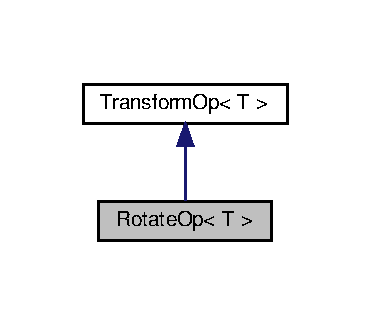
\includegraphics[width=187pt]{classRotateOp__inherit__graph}
\end{center}
\end{figure}


Collaboration diagram for Rotate\+Op$<$ T $>$\+:
\nopagebreak
\begin{figure}[H]
\begin{center}
\leavevmode
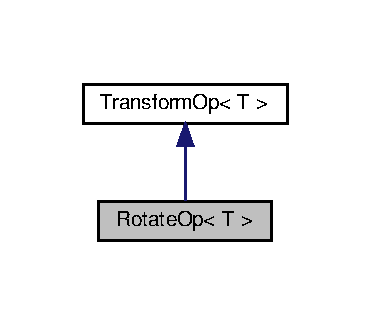
\includegraphics[width=187pt]{classRotateOp__coll__graph}
\end{center}
\end{figure}
\doxysubsection*{Public Member Functions}
\begin{DoxyCompactItemize}
\item 
\mbox{\Hypertarget{classRotateOp_afac8d44cae4c9109c96d2c1ae47a1dc2}\label{classRotateOp_afac8d44cae4c9109c96d2c1ae47a1dc2}} 
\mbox{\hyperlink{classRotateOp_afac8d44cae4c9109c96d2c1ae47a1dc2}{Rotate\+Op}} ()
\begin{DoxyCompactList}\small\item\em Weak constructor. \end{DoxyCompactList}\item 
\mbox{\hyperlink{classRotateOp_a9436aaf636bf136d9a80d91ae4a41659}{Rotate\+Op}} (const T a\+\_\+angle, const size\+\_\+t a\+\_\+axis) noexcept
\begin{DoxyCompactList}\small\item\em Full constructor. \end{DoxyCompactList}\item 
\mbox{\Hypertarget{classRotateOp_aaa12091fe7937f5ed7e2d35e0632337b}\label{classRotateOp_aaa12091fe7937f5ed7e2d35e0632337b}} 
virtual \mbox{\hyperlink{classRotateOp_aaa12091fe7937f5ed7e2d35e0632337b}{$\sim$\+Rotate\+Op}} ()=default
\begin{DoxyCompactList}\small\item\em Destructor. \end{DoxyCompactList}\item 
\mbox{\Hypertarget{classRotateOp_aaffc25806ef6b9d7ea6651aa2bb9767c}\label{classRotateOp_aaffc25806ef6b9d7ea6651aa2bb9767c}} 
\mbox{\hyperlink{classVec3T}{Vec3T}}$<$ T $>$ \mbox{\hyperlink{classRotateOp_aaffc25806ef6b9d7ea6651aa2bb9767c}{transform}} (const \mbox{\hyperlink{classVec3T}{Vec3T}}$<$ T $>$ \&a\+\_\+input\+Point) const noexcept override
\begin{DoxyCompactList}\small\item\em Transform input point. \end{DoxyCompactList}\end{DoxyCompactItemize}
\doxysubsection*{Protected Attributes}
\begin{DoxyCompactItemize}
\item 
\mbox{\Hypertarget{classRotateOp_ac1e23c3e185fe54f2e550c9eb52b1184}\label{classRotateOp_ac1e23c3e185fe54f2e550c9eb52b1184}} 
size\+\_\+t \mbox{\hyperlink{classRotateOp_ac1e23c3e185fe54f2e550c9eb52b1184}{m\+\_\+axis}}
\begin{DoxyCompactList}\small\item\em Rotation axis. 0 = x, 1=y etc. \end{DoxyCompactList}\item 
\mbox{\Hypertarget{classRotateOp_a8eed86f336946618f1964056405b9ac4}\label{classRotateOp_a8eed86f336946618f1964056405b9ac4}} 
T \mbox{\hyperlink{classRotateOp_a8eed86f336946618f1964056405b9ac4}{m\+\_\+cos\+Angle}}
\begin{DoxyCompactList}\small\item\em Theta-\/rotation (degrees) \end{DoxyCompactList}\item 
\mbox{\Hypertarget{classRotateOp_ab0f3316357239d07fb1da64b7298d53f}\label{classRotateOp_ab0f3316357239d07fb1da64b7298d53f}} 
T \mbox{\hyperlink{classRotateOp_ab0f3316357239d07fb1da64b7298d53f}{m\+\_\+sin\+Angle}}
\begin{DoxyCompactList}\small\item\em Phi-\/rotation (degrees) \end{DoxyCompactList}\end{DoxyCompactItemize}


\doxysubsection{Detailed Description}
\subsubsection*{template$<$class T$>$\newline
class Rotate\+Op$<$ T $>$}

Rotation operator. Can scale an input point. 

\doxysubsection{Constructor \& Destructor Documentation}
\mbox{\Hypertarget{classRotateOp_a9436aaf636bf136d9a80d91ae4a41659}\label{classRotateOp_a9436aaf636bf136d9a80d91ae4a41659}} 
\index{RotateOp$<$ T $>$@{RotateOp$<$ T $>$}!RotateOp@{RotateOp}}
\index{RotateOp@{RotateOp}!RotateOp$<$ T $>$@{RotateOp$<$ T $>$}}
\doxysubsubsection{\texorpdfstring{RotateOp()}{RotateOp()}}
{\footnotesize\ttfamily template$<$class T $>$ \\
\mbox{\hyperlink{classRotateOp}{Rotate\+Op}}$<$ T $>$\+::\mbox{\hyperlink{classRotateOp}{Rotate\+Op}} (\begin{DoxyParamCaption}\item[{const T}]{a\+\_\+angle,  }\item[{const size\+\_\+t}]{a\+\_\+axis }\end{DoxyParamCaption})\hspace{0.3cm}{\ttfamily [noexcept]}}



Full constructor. 


\begin{DoxyParams}[1]{Parameters}
\mbox{\texttt{ in}}  & {\em a\+\_\+angle} & Rotation angle \\
\hline
\mbox{\texttt{ in}}  & {\em a\+\_\+axis} & Rotation axis \\
\hline
\end{DoxyParams}


The documentation for this class was generated from the following files\+:\begin{DoxyCompactItemize}
\item 
/home/runner/work/\+E\+B\+Geometry/\+E\+B\+Geometry/\+Source/\mbox{\hyperlink{EBGeometry__TransformOps_8hpp}{E\+B\+Geometry\+\_\+\+Transform\+Ops.\+hpp}}\item 
/home/runner/work/\+E\+B\+Geometry/\+E\+B\+Geometry/\+Source/\mbox{\hyperlink{EBGeometry__TransformOpsImplem_8hpp}{E\+B\+Geometry\+\_\+\+Transform\+Ops\+Implem.\+hpp}}\end{DoxyCompactItemize}

\hypertarget{classScaleOp}{}\section{Scale\+Op$<$ T $>$ Class Template Reference}
\label{classScaleOp}\index{Scale\+Op$<$ T $>$@{Scale\+Op$<$ T $>$}}


Scale operator. Can also be used as a reflection operator.  




{\ttfamily \#include $<$E\+B\+Geometry\+\_\+\+Transform\+Ops.\+hpp$>$}



Inheritance diagram for Scale\+Op$<$ T $>$\+:\nopagebreak
\begin{figure}[H]
\begin{center}
\leavevmode
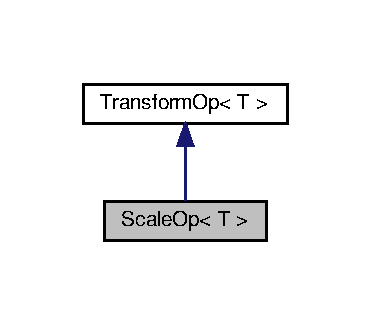
\includegraphics[width=178pt]{classScaleOp__inherit__graph}
\end{center}
\end{figure}


Collaboration diagram for Scale\+Op$<$ T $>$\+:\nopagebreak
\begin{figure}[H]
\begin{center}
\leavevmode
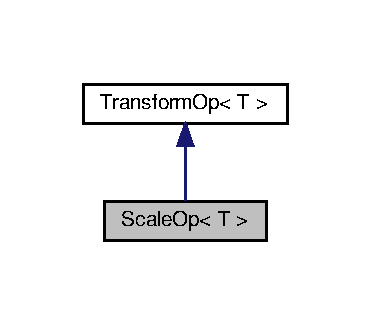
\includegraphics[width=178pt]{classScaleOp__coll__graph}
\end{center}
\end{figure}
\subsection*{Public Member Functions}
\begin{DoxyCompactItemize}
\item 
\mbox{\Hypertarget{classScaleOp_aaa6d5841955e1b0a883bbcb5fdcbddc6}\label{classScaleOp_aaa6d5841955e1b0a883bbcb5fdcbddc6}} 
\hyperlink{classScaleOp_aaa6d5841955e1b0a883bbcb5fdcbddc6}{Scale\+Op} ()
\begin{DoxyCompactList}\small\item\em Default constructor. \end{DoxyCompactList}\item 
\mbox{\Hypertarget{classScaleOp_ab556ea0d0521a8a153e2406b1255014e}\label{classScaleOp_ab556ea0d0521a8a153e2406b1255014e}} 
\hyperlink{classScaleOp_ab556ea0d0521a8a153e2406b1255014e}{Scale\+Op} (const \hyperlink{classVec3T}{Vec3T}$<$ T $>$ \&a\+\_\+scale)
\begin{DoxyCompactList}\small\item\em Full constructor. \end{DoxyCompactList}\item 
\mbox{\Hypertarget{classScaleOp_ab9fc71d00d7e0e339562edcaa2e3fc9a}\label{classScaleOp_ab9fc71d00d7e0e339562edcaa2e3fc9a}} 
virtual \hyperlink{classScaleOp_ab9fc71d00d7e0e339562edcaa2e3fc9a}{$\sim$\+Scale\+Op} ()=default
\begin{DoxyCompactList}\small\item\em Destructor. \end{DoxyCompactList}\item 
\mbox{\Hypertarget{classScaleOp_ac09e64516daa1b75111bd36dedfeeda9}\label{classScaleOp_ac09e64516daa1b75111bd36dedfeeda9}} 
\hyperlink{classVec3T}{Vec3T}$<$ T $>$ \hyperlink{classScaleOp_ac09e64516daa1b75111bd36dedfeeda9}{transform} (const \hyperlink{classVec3T}{Vec3T}$<$ T $>$ \&a\+\_\+input\+Point) const noexcept override
\begin{DoxyCompactList}\small\item\em Transform input point. \end{DoxyCompactList}\end{DoxyCompactItemize}
\subsection*{Protected Attributes}
\begin{DoxyCompactItemize}
\item 
\mbox{\Hypertarget{classScaleOp_aa9cdfff381b10970fd51eeb7e3e83188}\label{classScaleOp_aa9cdfff381b10970fd51eeb7e3e83188}} 
\hyperlink{classVec3T}{Vec3T}$<$ T $>$ \hyperlink{classScaleOp_aa9cdfff381b10970fd51eeb7e3e83188}{m\+\_\+scale}
\begin{DoxyCompactList}\small\item\em Scaling of input point. \end{DoxyCompactList}\end{DoxyCompactItemize}


\subsection{Detailed Description}
\subsubsection*{template$<$class T$>$\newline
class Scale\+Op$<$ T $>$}

Scale operator. Can also be used as a reflection operator. 

The documentation for this class was generated from the following files\+:\begin{DoxyCompactItemize}
\item 
Source/\hyperlink{EBGeometry__TransformOps_8hpp}{E\+B\+Geometry\+\_\+\+Transform\+Ops.\+hpp}\item 
Source/\hyperlink{EBGeometry__TransformOpsImplem_8hpp}{E\+B\+Geometry\+\_\+\+Transform\+Ops\+Implem.\+hpp}\end{DoxyCompactItemize}

\hypertarget{classSignedDistanceFunction}{}\doxysection{Signed\+Distance\+Function$<$ T $>$ Class Template Reference}
\label{classSignedDistanceFunction}\index{SignedDistanceFunction$<$ T $>$@{SignedDistanceFunction$<$ T $>$}}


Abstract representation of a signed distance function.  




{\ttfamily \#include $<$E\+B\+Geometry\+\_\+\+Signed\+Distance\+Function.\+hpp$>$}



Inheritance diagram for Signed\+Distance\+Function$<$ T $>$\+:
\nopagebreak
\begin{figure}[H]
\begin{center}
\leavevmode
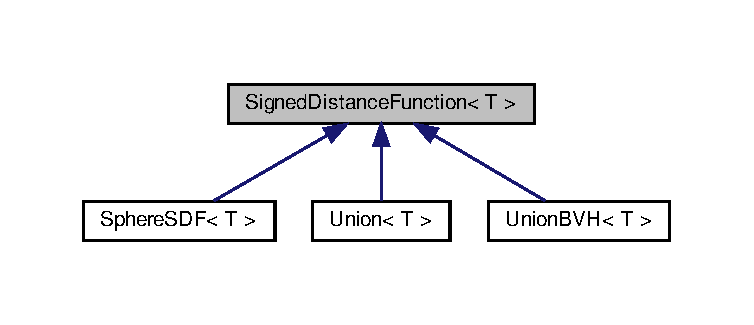
\includegraphics[width=350pt]{classSignedDistanceFunction__inherit__graph}
\end{center}
\end{figure}
\doxysubsection*{Public Member Functions}
\begin{DoxyCompactItemize}
\item 
\mbox{\Hypertarget{classSignedDistanceFunction_abfeeff9b3901e03ec6b73317dc9a722e}\label{classSignedDistanceFunction_abfeeff9b3901e03ec6b73317dc9a722e}} 
\mbox{\hyperlink{classSignedDistanceFunction_abfeeff9b3901e03ec6b73317dc9a722e}{Signed\+Distance\+Function}} ()=default
\begin{DoxyCompactList}\small\item\em Disallowed, use the full constructor. \end{DoxyCompactList}\item 
\mbox{\Hypertarget{classSignedDistanceFunction_ab47b289bd8351d7f323938c91b2bb92b}\label{classSignedDistanceFunction_ab47b289bd8351d7f323938c91b2bb92b}} 
virtual \mbox{\hyperlink{classSignedDistanceFunction_ab47b289bd8351d7f323938c91b2bb92b}{$\sim$\+Signed\+Distance\+Function}} ()=default
\begin{DoxyCompactList}\small\item\em Destructor (does nothing) \end{DoxyCompactList}\item 
virtual T \mbox{\hyperlink{classSignedDistanceFunction_af5912280ca51dc21a2d6949a30ec7d21}{signed\+Distance}} (const \mbox{\hyperlink{classVec3T}{Vec3T}}$<$ T $>$ \&a\+\_\+point) const noexcept=0
\begin{DoxyCompactList}\small\item\em Signed distance function. \end{DoxyCompactList}\item 
virtual \mbox{\hyperlink{classVec3T}{Vec3T}}$<$ T $>$ \mbox{\hyperlink{classSignedDistanceFunction_ae9f55561cebcd7b2eafc1e2e3ae44027}{normal}} (const \mbox{\hyperlink{classVec3T}{Vec3T}}$<$ T $>$ \&a\+\_\+point, const T \&a\+\_\+delta) const noexcept
\begin{DoxyCompactList}\small\item\em Signed distance normal vector. \end{DoxyCompactList}\item 
void \mbox{\hyperlink{classSignedDistanceFunction_add71ebc2e7f3fb5e85766898413482e7}{translate}} (const \mbox{\hyperlink{classVec3T}{Vec3T}}$<$ T $>$ \&a\+\_\+translation) noexcept
\begin{DoxyCompactList}\small\item\em Translate signed distance function. \end{DoxyCompactList}\item 
void \mbox{\hyperlink{classSignedDistanceFunction_ae8de697f4d0966290342bcf6383585ef}{rotate}} (const T a\+\_\+angle, const int a\+\_\+axis) noexcept
\begin{DoxyCompactList}\small\item\em Rotate the signed distance function around. \end{DoxyCompactList}\end{DoxyCompactItemize}
\doxysubsection*{Protected Member Functions}
\begin{DoxyCompactItemize}
\item 
\mbox{\Hypertarget{classSignedDistanceFunction_af186f98f9ea4ac96fccb4add4ebf196d}\label{classSignedDistanceFunction_af186f98f9ea4ac96fccb4add4ebf196d}} 
\mbox{\hyperlink{classVec3T}{Vec3T}}$<$ T $>$ \mbox{\hyperlink{classSignedDistanceFunction_af186f98f9ea4ac96fccb4add4ebf196d}{transform\+Point}} (const \mbox{\hyperlink{classVec3T}{Vec3T}}$<$ T $>$ \&a\+\_\+point) const noexcept
\begin{DoxyCompactList}\small\item\em Apply transformation operators and move point. \end{DoxyCompactList}\end{DoxyCompactItemize}
\doxysubsection*{Protected Attributes}
\begin{DoxyCompactItemize}
\item 
\mbox{\Hypertarget{classSignedDistanceFunction_af61e5e2ece6add9d2bcf8e5aa8cf2844}\label{classSignedDistanceFunction_af61e5e2ece6add9d2bcf8e5aa8cf2844}} 
std\+::deque$<$ std\+::shared\+\_\+ptr$<$ \mbox{\hyperlink{classTransformOp}{Transform\+Op}}$<$ T $>$ $>$ $>$ \mbox{\hyperlink{classSignedDistanceFunction_af61e5e2ece6add9d2bcf8e5aa8cf2844}{m\+\_\+transform\+Ops}}
\begin{DoxyCompactList}\small\item\em List of transformation operators for the signed distance field. \end{DoxyCompactList}\end{DoxyCompactItemize}


\doxysubsection{Detailed Description}
\subsubsection*{template$<$class T$>$\newline
class Signed\+Distance\+Function$<$ T $>$}

Abstract representation of a signed distance function. 

Users can put whatever they like in here, e.\+g. analytic functions, D\+C\+EL meshes, or D\+C\+EL meshes stored in full or compact \mbox{\hyperlink{namespaceBVH}{B\+VH}} trees. The signed\+Distance function must be implemented by the user. When computing it, the user can apply transformation operators (rotations, scaling, translations) by calling transform\+Point on the input coordinate. 

\doxysubsection{Member Function Documentation}
\mbox{\Hypertarget{classSignedDistanceFunction_ae9f55561cebcd7b2eafc1e2e3ae44027}\label{classSignedDistanceFunction_ae9f55561cebcd7b2eafc1e2e3ae44027}} 
\index{SignedDistanceFunction$<$ T $>$@{SignedDistanceFunction$<$ T $>$}!normal@{normal}}
\index{normal@{normal}!SignedDistanceFunction$<$ T $>$@{SignedDistanceFunction$<$ T $>$}}
\doxysubsubsection{\texorpdfstring{normal()}{normal()}}
{\footnotesize\ttfamily template$<$class T $>$ \\
\mbox{\hyperlink{classVec3T}{Vec3T}}$<$ T $>$ \mbox{\hyperlink{classSignedDistanceFunction}{Signed\+Distance\+Function}}$<$ T $>$\+::normal (\begin{DoxyParamCaption}\item[{const \mbox{\hyperlink{classVec3T}{Vec3T}}$<$ T $>$ \&}]{a\+\_\+point,  }\item[{const T \&}]{a\+\_\+delta }\end{DoxyParamCaption}) const\hspace{0.3cm}{\ttfamily [inline]}, {\ttfamily [virtual]}, {\ttfamily [noexcept]}}



Signed distance normal vector. 

Computed using finite differences with step a\+\_\+delta 
\begin{DoxyParams}[1]{Parameters}
\mbox{\texttt{ in}}  & {\em a\+\_\+point} & 3D point \\
\hline
\mbox{\texttt{ in}}  & {\em a\+\_\+delta} & Finite difference step \\
\hline
\end{DoxyParams}
\mbox{\Hypertarget{classSignedDistanceFunction_ae8de697f4d0966290342bcf6383585ef}\label{classSignedDistanceFunction_ae8de697f4d0966290342bcf6383585ef}} 
\index{SignedDistanceFunction$<$ T $>$@{SignedDistanceFunction$<$ T $>$}!rotate@{rotate}}
\index{rotate@{rotate}!SignedDistanceFunction$<$ T $>$@{SignedDistanceFunction$<$ T $>$}}
\doxysubsubsection{\texorpdfstring{rotate()}{rotate()}}
{\footnotesize\ttfamily template$<$class T $>$ \\
void \mbox{\hyperlink{classSignedDistanceFunction}{Signed\+Distance\+Function}}$<$ T $>$\+::rotate (\begin{DoxyParamCaption}\item[{const T}]{a\+\_\+angle,  }\item[{const int}]{a\+\_\+axis }\end{DoxyParamCaption})\hspace{0.3cm}{\ttfamily [inline]}, {\ttfamily [noexcept]}}



Rotate the signed distance function around. 


\begin{DoxyParams}[1]{Parameters}
\mbox{\texttt{ in}}  & {\em a\+\_\+angle} & Rotation angle \\
\hline
\mbox{\texttt{ in}}  & {\em a\+\_\+axis} & Rotation axis. 0 = x, 1 = y etc. \\
\hline
\end{DoxyParams}
\mbox{\Hypertarget{classSignedDistanceFunction_af5912280ca51dc21a2d6949a30ec7d21}\label{classSignedDistanceFunction_af5912280ca51dc21a2d6949a30ec7d21}} 
\index{SignedDistanceFunction$<$ T $>$@{SignedDistanceFunction$<$ T $>$}!signedDistance@{signedDistance}}
\index{signedDistance@{signedDistance}!SignedDistanceFunction$<$ T $>$@{SignedDistanceFunction$<$ T $>$}}
\doxysubsubsection{\texorpdfstring{signedDistance()}{signedDistance()}}
{\footnotesize\ttfamily template$<$class T $>$ \\
virtual T \mbox{\hyperlink{classSignedDistanceFunction}{Signed\+Distance\+Function}}$<$ T $>$\+::signed\+Distance (\begin{DoxyParamCaption}\item[{const \mbox{\hyperlink{classVec3T}{Vec3T}}$<$ T $>$ \&}]{a\+\_\+point }\end{DoxyParamCaption}) const\hspace{0.3cm}{\ttfamily [pure virtual]}, {\ttfamily [noexcept]}}



Signed distance function. 


\begin{DoxyParams}[1]{Parameters}
\mbox{\texttt{ in}}  & {\em a\+\_\+point} & 3D point. \\
\hline
\end{DoxyParams}


Implemented in \mbox{\hyperlink{classConeSDF_a4ef38df98e9831c25297cb93a5b41da5}{Cone\+S\+D\+F$<$ T $>$}}, \mbox{\hyperlink{classInfiniteConeSDF_a98232920c669d548b84493d9e55ddc0a}{Infinite\+Cone\+S\+D\+F$<$ T $>$}}, \mbox{\hyperlink{classCapsuleSDF_a2fa33052a5d93eb0f7fb0a6ff32122e9}{Capsule\+S\+D\+F$<$ T $>$}}, \mbox{\hyperlink{classInfiniteCylinderSDF_a2481e68ea21c304c858878ae1d7fc031}{Infinite\+Cylinder\+S\+D\+F$<$ T $>$}}, \mbox{\hyperlink{classCylinderSDF_a082c08089b07402d55020ed8186cc992}{Cylinder\+S\+D\+F$<$ T $>$}}, \mbox{\hyperlink{classTorusSDF_a23b4d455de2b7b9988ce81833ccd5302}{Torus\+S\+D\+F$<$ T $>$}}, \mbox{\hyperlink{classBoxSDF_a6e7a72790061423e5c9ea47d9e26736f}{Box\+S\+D\+F$<$ T $>$}}, \mbox{\hyperlink{classSphereSDF_a9b0c5f0b1af2c4b62bee1c873e0158e8}{Sphere\+S\+D\+F$<$ T $>$}}, \mbox{\hyperlink{classPlaneSDF_a75c2d73156caac10eefce9b431542d88}{Plane\+S\+D\+F$<$ T $>$}}, \mbox{\hyperlink{classScaledSDF_aeb8f6c22a2f9f242b171a928db1f0069}{Scaled\+S\+D\+F$<$ T $>$}}, \mbox{\hyperlink{classAnnularSDF_ab933bf07072202ccc1e3bbb59bc49465}{Annular\+S\+D\+F$<$ T $>$}}, \mbox{\hyperlink{classUnionBVH_a9681fdc161e2e077a33caaddb78fb4ba}{Union\+B\+V\+H$<$ T, B\+V, K $>$}}, \mbox{\hyperlink{classRoundedSDF_a3e59b861e66c4398a7a0cc8ecda0e318}{Rounded\+S\+D\+F$<$ T $>$}}, and \mbox{\hyperlink{classUnion_a08beffd354ca261e3d31bcb453951810}{Union$<$ T $>$}}.

\mbox{\Hypertarget{classSignedDistanceFunction_add71ebc2e7f3fb5e85766898413482e7}\label{classSignedDistanceFunction_add71ebc2e7f3fb5e85766898413482e7}} 
\index{SignedDistanceFunction$<$ T $>$@{SignedDistanceFunction$<$ T $>$}!translate@{translate}}
\index{translate@{translate}!SignedDistanceFunction$<$ T $>$@{SignedDistanceFunction$<$ T $>$}}
\doxysubsubsection{\texorpdfstring{translate()}{translate()}}
{\footnotesize\ttfamily template$<$class T $>$ \\
void \mbox{\hyperlink{classSignedDistanceFunction}{Signed\+Distance\+Function}}$<$ T $>$\+::translate (\begin{DoxyParamCaption}\item[{const \mbox{\hyperlink{classVec3T}{Vec3T}}$<$ T $>$ \&}]{a\+\_\+translation }\end{DoxyParamCaption})\hspace{0.3cm}{\ttfamily [inline]}, {\ttfamily [noexcept]}}



Translate signed distance function. 


\begin{DoxyParams}[1]{Parameters}
\mbox{\texttt{ in}}  & {\em a\+\_\+translation} & Distance to translate the function. \\
\hline
\end{DoxyParams}


The documentation for this class was generated from the following files\+:\begin{DoxyCompactItemize}
\item 
Source/\mbox{\hyperlink{EBGeometry__SignedDistanceFunction_8hpp}{E\+B\+Geometry\+\_\+\+Signed\+Distance\+Function.\+hpp}}\item 
Source/\mbox{\hyperlink{EBGeometry__SignedDistanceFunctionImplem_8hpp}{E\+B\+Geometry\+\_\+\+Signed\+Distance\+Function\+Implem.\+hpp}}\end{DoxyCompactItemize}

\hypertarget{classSphereSDF}{}\doxysection{Sphere\+SDF$<$ T $>$ Class Template Reference}
\label{classSphereSDF}\index{SphereSDF$<$ T $>$@{SphereSDF$<$ T $>$}}


Signed distance field for sphere.  




{\ttfamily \#include $<$EBGeometry\+\_\+\+Analytic\+Distance\+Functions.\+hpp$>$}



Inheritance diagram for Sphere\+SDF$<$ T $>$\+:
\nopagebreak
\begin{figure}[H]
\begin{center}
\leavevmode
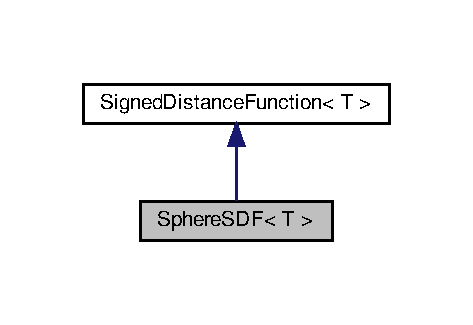
\includegraphics[width=242pt]{classSphereSDF__inherit__graph}
\end{center}
\end{figure}


Collaboration diagram for Sphere\+SDF$<$ T $>$\+:
\nopagebreak
\begin{figure}[H]
\begin{center}
\leavevmode
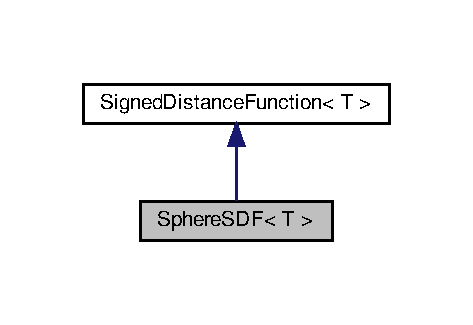
\includegraphics[width=242pt]{classSphereSDF__coll__graph}
\end{center}
\end{figure}
\doxysubsection*{Public Member Functions}
\begin{DoxyCompactItemize}
\item 
\mbox{\Hypertarget{classSphereSDF_ad5f6d20f6ccd77ba91c00acd2aeea28f}\label{classSphereSDF_ad5f6d20f6ccd77ba91c00acd2aeea28f}} 
\mbox{\hyperlink{classSphereSDF_ad5f6d20f6ccd77ba91c00acd2aeea28f}{Sphere\+SDF}} ()=delete
\begin{DoxyCompactList}\small\item\em Disallowed weak construction. \end{DoxyCompactList}\item 
\mbox{\hyperlink{classSphereSDF_a5b655d372efcf2aaf161930ed59c9021}{Sphere\+SDF}} (const \mbox{\hyperlink{classVec3T}{Vec3T}}$<$ T $>$ \&a\+\_\+center, const T \&a\+\_\+radius) noexcept
\begin{DoxyCompactList}\small\item\em Default constructor. \end{DoxyCompactList}\item 
\mbox{\Hypertarget{classSphereSDF_aa8b1dc622a46ec731d614eee53baa530}\label{classSphereSDF_aa8b1dc622a46ec731d614eee53baa530}} 
\mbox{\hyperlink{classSphereSDF_aa8b1dc622a46ec731d614eee53baa530}{Sphere\+SDF}} (const \mbox{\hyperlink{classSphereSDF}{Sphere\+SDF}} \&a\+\_\+other) noexcept
\begin{DoxyCompactList}\small\item\em Copy constructor. \end{DoxyCompactList}\item 
\mbox{\Hypertarget{classSphereSDF_a287e108c767242ef66004a43ed904054}\label{classSphereSDF_a287e108c767242ef66004a43ed904054}} 
virtual \mbox{\hyperlink{classSphereSDF_a287e108c767242ef66004a43ed904054}{$\sim$\+Sphere\+SDF}} () noexcept=default
\begin{DoxyCompactList}\small\item\em Destructor. \end{DoxyCompactList}\item 
\mbox{\Hypertarget{classSphereSDF_a82922ae162a9b96279cc4d0d866b303d}\label{classSphereSDF_a82922ae162a9b96279cc4d0d866b303d}} 
const \mbox{\hyperlink{classVec3T}{Vec3T}}$<$ T $>$ \& \mbox{\hyperlink{classSphereSDF_a82922ae162a9b96279cc4d0d866b303d}{get\+Center}} () const noexcept
\begin{DoxyCompactList}\small\item\em Get center. \end{DoxyCompactList}\item 
\mbox{\Hypertarget{classSphereSDF_a4f3a9220bfe2fc817131f655ce6f30cd}\label{classSphereSDF_a4f3a9220bfe2fc817131f655ce6f30cd}} 
\mbox{\hyperlink{classVec3T}{Vec3T}}$<$ T $>$ \& \mbox{\hyperlink{classSphereSDF_a4f3a9220bfe2fc817131f655ce6f30cd}{get\+Center}} () noexcept
\begin{DoxyCompactList}\small\item\em Get center. \end{DoxyCompactList}\item 
\mbox{\Hypertarget{classSphereSDF_a2cdc1f42f3de4c0ca017571910fbe72c}\label{classSphereSDF_a2cdc1f42f3de4c0ca017571910fbe72c}} 
const T \& \mbox{\hyperlink{classSphereSDF_a2cdc1f42f3de4c0ca017571910fbe72c}{get\+Radius}} () const noexcept
\begin{DoxyCompactList}\small\item\em Get radius. \end{DoxyCompactList}\item 
\mbox{\Hypertarget{classSphereSDF_a09245289037ae77adf204160c0d5b9cc}\label{classSphereSDF_a09245289037ae77adf204160c0d5b9cc}} 
T \& \mbox{\hyperlink{classSphereSDF_a09245289037ae77adf204160c0d5b9cc}{get\+Radius}} () noexcept
\begin{DoxyCompactList}\small\item\em Get radius. \end{DoxyCompactList}\item 
virtual T \mbox{\hyperlink{classSphereSDF_a9b0c5f0b1af2c4b62bee1c873e0158e8}{signed\+Distance}} (const \mbox{\hyperlink{classVec3T}{Vec3T}}$<$ T $>$ \&a\+\_\+point) const noexcept override
\begin{DoxyCompactList}\small\item\em Signed distance function for sphere. \end{DoxyCompactList}\end{DoxyCompactItemize}
\doxysubsection*{Protected Attributes}
\begin{DoxyCompactItemize}
\item 
\mbox{\Hypertarget{classSphereSDF_ab3caacb26a72b3ada01f09a248f5cb83}\label{classSphereSDF_ab3caacb26a72b3ada01f09a248f5cb83}} 
\mbox{\hyperlink{classVec3T}{Vec3T}}$<$ T $>$ \mbox{\hyperlink{classSphereSDF_ab3caacb26a72b3ada01f09a248f5cb83}{m\+\_\+center}}
\begin{DoxyCompactList}\small\item\em Sphere center. \end{DoxyCompactList}\item 
\mbox{\Hypertarget{classSphereSDF_ac4b0f786ea2b53530512ce3fa4e7bdbd}\label{classSphereSDF_ac4b0f786ea2b53530512ce3fa4e7bdbd}} 
T \mbox{\hyperlink{classSphereSDF_ac4b0f786ea2b53530512ce3fa4e7bdbd}{m\+\_\+radius}}
\begin{DoxyCompactList}\small\item\em Sphere radius. \end{DoxyCompactList}\end{DoxyCompactItemize}


\doxysubsection{Detailed Description}
\subsubsection*{template$<$class T$>$\newline
class Sphere\+SDF$<$ T $>$}

Signed distance field for sphere. 

\doxysubsection{Constructor \& Destructor Documentation}
\mbox{\Hypertarget{classSphereSDF_a5b655d372efcf2aaf161930ed59c9021}\label{classSphereSDF_a5b655d372efcf2aaf161930ed59c9021}} 
\index{SphereSDF$<$ T $>$@{SphereSDF$<$ T $>$}!SphereSDF@{SphereSDF}}
\index{SphereSDF@{SphereSDF}!SphereSDF$<$ T $>$@{SphereSDF$<$ T $>$}}
\doxysubsubsection{\texorpdfstring{SphereSDF()}{SphereSDF()}}
{\footnotesize\ttfamily template$<$class T $>$ \\
\mbox{\hyperlink{classSphereSDF}{Sphere\+SDF}}$<$ T $>$\+::\mbox{\hyperlink{classSphereSDF}{Sphere\+SDF}} (\begin{DoxyParamCaption}\item[{const \mbox{\hyperlink{classVec3T}{Vec3T}}$<$ T $>$ \&}]{a\+\_\+center,  }\item[{const T \&}]{a\+\_\+radius }\end{DoxyParamCaption})\hspace{0.3cm}{\ttfamily [inline]}, {\ttfamily [noexcept]}}



Default constructor. 


\begin{DoxyParams}[1]{Parameters}
\mbox{\texttt{ in}}  & {\em a\+\_\+center} & Sphere center \\
\hline
\mbox{\texttt{ in}}  & {\em a\+\_\+radius} & Sphere radius \\
\hline
\end{DoxyParams}


\doxysubsection{Member Function Documentation}
\mbox{\Hypertarget{classSphereSDF_a9b0c5f0b1af2c4b62bee1c873e0158e8}\label{classSphereSDF_a9b0c5f0b1af2c4b62bee1c873e0158e8}} 
\index{SphereSDF$<$ T $>$@{SphereSDF$<$ T $>$}!signedDistance@{signedDistance}}
\index{signedDistance@{signedDistance}!SphereSDF$<$ T $>$@{SphereSDF$<$ T $>$}}
\doxysubsubsection{\texorpdfstring{signedDistance()}{signedDistance()}}
{\footnotesize\ttfamily template$<$class T $>$ \\
virtual T \mbox{\hyperlink{classSphereSDF}{Sphere\+SDF}}$<$ T $>$\+::signed\+Distance (\begin{DoxyParamCaption}\item[{const \mbox{\hyperlink{classVec3T}{Vec3T}}$<$ T $>$ \&}]{a\+\_\+point }\end{DoxyParamCaption}) const\hspace{0.3cm}{\ttfamily [inline]}, {\ttfamily [override]}, {\ttfamily [virtual]}, {\ttfamily [noexcept]}}



Signed distance function for sphere. 


\begin{DoxyParams}[1]{Parameters}
\mbox{\texttt{ in}}  & {\em a\+\_\+point} & Position. \\
\hline
\end{DoxyParams}


Implements \mbox{\hyperlink{classSignedDistanceFunction_af5912280ca51dc21a2d6949a30ec7d21}{Signed\+Distance\+Function$<$ T $>$}}.



The documentation for this class was generated from the following file\+:\begin{DoxyCompactItemize}
\item 
/home/runner/work/\+EBGeometry/\+EBGeometry/\+Source/\mbox{\hyperlink{EBGeometry__AnalyticDistanceFunctions_8hpp}{EBGeometry\+\_\+\+Analytic\+Distance\+Functions.\+hpp}}\end{DoxyCompactItemize}

\hypertarget{classTransformOp}{}\section{Transform\+Op$<$ T $>$ Class Template Reference}
\label{classTransformOp}\index{Transform\+Op$<$ T $>$@{Transform\+Op$<$ T $>$}}


Base class for transformation operators.  




{\ttfamily \#include $<$E\+B\+Geometry\+\_\+\+Transform\+Ops.\+hpp$>$}



Inheritance diagram for Transform\+Op$<$ T $>$\+:
\nopagebreak
\begin{figure}[H]
\begin{center}
\leavevmode
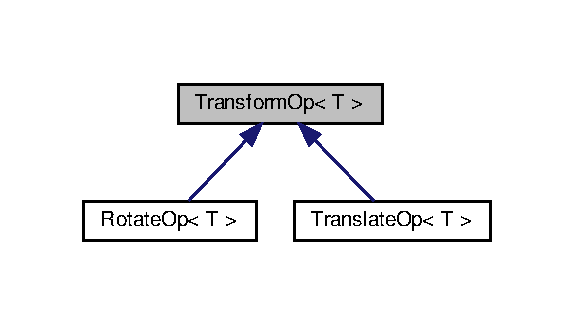
\includegraphics[width=276pt]{classTransformOp__inherit__graph}
\end{center}
\end{figure}
\subsection*{Public Member Functions}
\begin{DoxyCompactItemize}
\item 
\mbox{\Hypertarget{classTransformOp_ab904cbdd373ca07e08b254163331b3b4}\label{classTransformOp_ab904cbdd373ca07e08b254163331b3b4}} 
\hyperlink{classTransformOp_ab904cbdd373ca07e08b254163331b3b4}{Transform\+Op} ()=default
\begin{DoxyCompactList}\small\item\em Default constructor. \end{DoxyCompactList}\item 
\mbox{\Hypertarget{classTransformOp_a556cc7f5bbe70ce148a0791b883eb58c}\label{classTransformOp_a556cc7f5bbe70ce148a0791b883eb58c}} 
virtual \hyperlink{classTransformOp_a556cc7f5bbe70ce148a0791b883eb58c}{$\sim$\+Transform\+Op} ()=default
\begin{DoxyCompactList}\small\item\em Destructor. \end{DoxyCompactList}\item 
virtual \hyperlink{classVec3T}{Vec3T}$<$ T $>$ \hyperlink{classTransformOp_a61c1920daa9f55fd2ea9095cbcfa18b8}{transform} (const \hyperlink{classVec3T}{Vec3T}$<$ T $>$ \&a\+\_\+input\+Point) const noexcept=0
\begin{DoxyCompactList}\small\item\em Transform input coordinate. \end{DoxyCompactList}\end{DoxyCompactItemize}


\subsection{Detailed Description}
\subsubsection*{template$<$class T$>$\newline
class Transform\+Op$<$ T $>$}

Base class for transformation operators. 

\subsection{Member Function Documentation}
\mbox{\Hypertarget{classTransformOp_a61c1920daa9f55fd2ea9095cbcfa18b8}\label{classTransformOp_a61c1920daa9f55fd2ea9095cbcfa18b8}} 
\index{Transform\+Op@{Transform\+Op}!transform@{transform}}
\index{transform@{transform}!Transform\+Op@{Transform\+Op}}
\subsubsection{\texorpdfstring{transform()}{transform()}}
{\footnotesize\ttfamily template$<$class T $>$ \\
virtual \hyperlink{classVec3T}{Vec3T}$<$T$>$ \hyperlink{classTransformOp}{Transform\+Op}$<$ T $>$\+::transform (\begin{DoxyParamCaption}\item[{const \hyperlink{classVec3T}{Vec3T}$<$ T $>$ \&}]{a\+\_\+input\+Point }\end{DoxyParamCaption}) const\hspace{0.3cm}{\ttfamily [pure virtual]}, {\ttfamily [noexcept]}}



Transform input coordinate. 


\begin{DoxyParams}[1]{Parameters}
\mbox{\tt in}  & {\em a\+\_\+input\+Point} & Input point \\
\hline
\end{DoxyParams}
\begin{DoxyReturn}{Returns}
Returns transformed point. 
\end{DoxyReturn}


Implemented in \hyperlink{classRotateOp_aaffc25806ef6b9d7ea6651aa2bb9767c}{Rotate\+Op$<$ T $>$}, and \hyperlink{classTranslateOp_a16941d9e52b02d39f9c92f6b23f61af6}{Translate\+Op$<$ T $>$}.



The documentation for this class was generated from the following file\+:\begin{DoxyCompactItemize}
\item 
Source/\hyperlink{EBGeometry__TransformOps_8hpp}{E\+B\+Geometry\+\_\+\+Transform\+Ops.\+hpp}\end{DoxyCompactItemize}

\hypertarget{classTranslateOp}{}\doxysection{Translate\+Op$<$ T $>$ Class Template Reference}
\label{classTranslateOp}\index{TranslateOp$<$ T $>$@{TranslateOp$<$ T $>$}}


Translation operator. Can translate an input point.  




{\ttfamily \#include $<$E\+B\+Geometry\+\_\+\+Transform\+Ops.\+hpp$>$}



Inheritance diagram for Translate\+Op$<$ T $>$\+:
\nopagebreak
\begin{figure}[H]
\begin{center}
\leavevmode
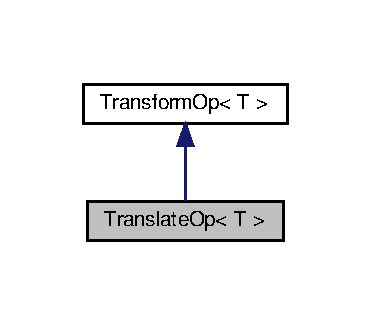
\includegraphics[width=187pt]{classTranslateOp__inherit__graph}
\end{center}
\end{figure}


Collaboration diagram for Translate\+Op$<$ T $>$\+:
\nopagebreak
\begin{figure}[H]
\begin{center}
\leavevmode
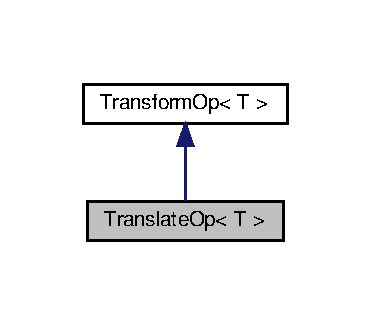
\includegraphics[width=187pt]{classTranslateOp__coll__graph}
\end{center}
\end{figure}
\doxysubsection*{Public Member Functions}
\begin{DoxyCompactItemize}
\item 
\mbox{\Hypertarget{classTranslateOp_ab20f5a272d6cd34bf98fc23523913fc9}\label{classTranslateOp_ab20f5a272d6cd34bf98fc23523913fc9}} 
\mbox{\hyperlink{classTranslateOp_ab20f5a272d6cd34bf98fc23523913fc9}{Translate\+Op}} ()
\begin{DoxyCompactList}\small\item\em Default constructor. \end{DoxyCompactList}\item 
\mbox{\Hypertarget{classTranslateOp_ac646a47f26119d8316533c91f3043864}\label{classTranslateOp_ac646a47f26119d8316533c91f3043864}} 
\mbox{\hyperlink{classTranslateOp_ac646a47f26119d8316533c91f3043864}{Translate\+Op}} (const \mbox{\hyperlink{classVec3T}{Vec3T}}$<$ T $>$ \&a\+\_\+translation)
\begin{DoxyCompactList}\small\item\em Full constructor. \end{DoxyCompactList}\item 
\mbox{\Hypertarget{classTranslateOp_ad96b4ec0f30fb98dbd684afef1bfff03}\label{classTranslateOp_ad96b4ec0f30fb98dbd684afef1bfff03}} 
virtual \mbox{\hyperlink{classTranslateOp_ad96b4ec0f30fb98dbd684afef1bfff03}{$\sim$\+Translate\+Op}} ()=default
\begin{DoxyCompactList}\small\item\em Destructor. \end{DoxyCompactList}\item 
\mbox{\Hypertarget{classTranslateOp_a16941d9e52b02d39f9c92f6b23f61af6}\label{classTranslateOp_a16941d9e52b02d39f9c92f6b23f61af6}} 
\mbox{\hyperlink{classVec3T}{Vec3T}}$<$ T $>$ \mbox{\hyperlink{classTranslateOp_a16941d9e52b02d39f9c92f6b23f61af6}{transform}} (const \mbox{\hyperlink{classVec3T}{Vec3T}}$<$ T $>$ \&a\+\_\+input\+Point) const noexcept override
\begin{DoxyCompactList}\small\item\em Transform input point. \end{DoxyCompactList}\end{DoxyCompactItemize}
\doxysubsection*{Protected Attributes}
\begin{DoxyCompactItemize}
\item 
\mbox{\Hypertarget{classTranslateOp_a35f16c6a9cf4c03edffa19d86e73d27a}\label{classTranslateOp_a35f16c6a9cf4c03edffa19d86e73d27a}} 
\mbox{\hyperlink{classVec3T}{Vec3T}}$<$ T $>$ \mbox{\hyperlink{classTranslateOp_a35f16c6a9cf4c03edffa19d86e73d27a}{m\+\_\+translation}}
\begin{DoxyCompactList}\small\item\em Translation of input point. \end{DoxyCompactList}\end{DoxyCompactItemize}


\doxysubsection{Detailed Description}
\subsubsection*{template$<$class T$>$\newline
class Translate\+Op$<$ T $>$}

Translation operator. Can translate an input point. 

The documentation for this class was generated from the following files\+:\begin{DoxyCompactItemize}
\item 
/home/runner/work/\+E\+B\+Geometry/\+E\+B\+Geometry/\+Source/\mbox{\hyperlink{EBGeometry__TransformOps_8hpp}{E\+B\+Geometry\+\_\+\+Transform\+Ops.\+hpp}}\item 
/home/runner/work/\+E\+B\+Geometry/\+E\+B\+Geometry/\+Source/\mbox{\hyperlink{EBGeometry__TransformOpsImplem_8hpp}{E\+B\+Geometry\+\_\+\+Transform\+Ops\+Implem.\+hpp}}\end{DoxyCompactItemize}

\hypertarget{classUnion}{}\doxysection{Union$<$ T, P $>$ Class Template Reference}
\label{classUnion}\index{Union$<$ T, P $>$@{Union$<$ T, P $>$}}


CSG union. Computes the minimum of all input primitives. This is defined also when objects in the scene overlap one another. It will also.  




{\ttfamily \#include $<$EBGeometry\+\_\+\+Union.\+hpp$>$}



Inheritance diagram for Union$<$ T, P $>$\+:
\nopagebreak
\begin{figure}[H]
\begin{center}
\leavevmode
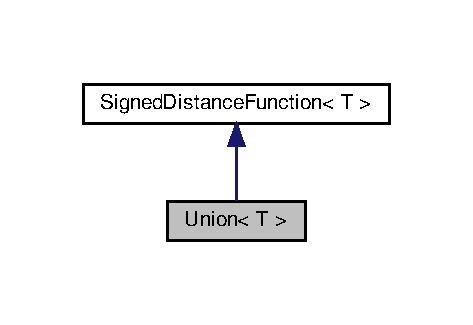
\includegraphics[width=203pt]{classUnion__inherit__graph}
\end{center}
\end{figure}


Collaboration diagram for Union$<$ T, P $>$\+:
\nopagebreak
\begin{figure}[H]
\begin{center}
\leavevmode
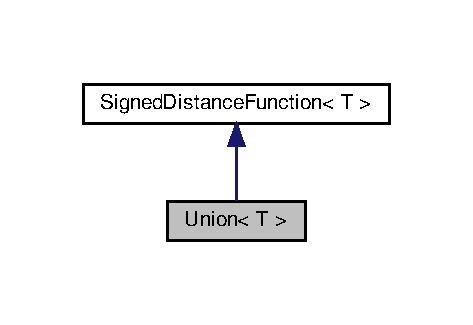
\includegraphics[width=203pt]{classUnion__coll__graph}
\end{center}
\end{figure}
\doxysubsection*{Public Member Functions}
\begin{DoxyCompactItemize}
\item 
\mbox{\Hypertarget{classUnion_aa8c4c6acaa20bf3c16ec105f1a123e11}\label{classUnion_aa8c4c6acaa20bf3c16ec105f1a123e11}} 
\mbox{\hyperlink{classUnion_aa8c4c6acaa20bf3c16ec105f1a123e11}{Union}} ()=delete
\begin{DoxyCompactList}\small\item\em Disallowed, use the full constructor. \end{DoxyCompactList}\item 
\mbox{\hyperlink{classUnion_ab21d9b892f4e9d9aa79277f3ad4032bf}{Union}} (const std\+::vector$<$ std\+::shared\+\_\+ptr$<$ P $>$$>$ \&a\+\_\+primitives, const bool a\+\_\+flip\+Sign)
\begin{DoxyCompactList}\small\item\em Full constructor. Computes the CSG union. \end{DoxyCompactList}\item 
\mbox{\Hypertarget{classUnion_af11948ba4db9a93446bde819f31f49ce}\label{classUnion_af11948ba4db9a93446bde819f31f49ce}} 
virtual \mbox{\hyperlink{classUnion_af11948ba4db9a93446bde819f31f49ce}{$\sim$\+Union}} ()=default
\begin{DoxyCompactList}\small\item\em Destructor (does nothing) \end{DoxyCompactList}\item 
T \mbox{\hyperlink{classUnion_af7d14a7b9a916489f2dfb16ffa3da5b2}{value}} (const \mbox{\hyperlink{classVec3T}{Vec3T}}$<$ T $>$ \&a\+\_\+point) const noexcept override
\begin{DoxyCompactList}\small\item\em Value function. \end{DoxyCompactList}\end{DoxyCompactItemize}
\doxysubsection*{Protected Attributes}
\begin{DoxyCompactItemize}
\item 
\mbox{\Hypertarget{classUnion_ad59e877314c00c35b366a463b05062f8}\label{classUnion_ad59e877314c00c35b366a463b05062f8}} 
std\+::vector$<$ std\+::shared\+\_\+ptr$<$ const P $>$ $>$ \mbox{\hyperlink{classUnion_ad59e877314c00c35b366a463b05062f8}{m\+\_\+primitives}}
\begin{DoxyCompactList}\small\item\em List of primitives. \end{DoxyCompactList}\item 
\mbox{\Hypertarget{classUnion_a2ea42d9aa14c07c50a132d35d5b9ef8f}\label{classUnion_a2ea42d9aa14c07c50a132d35d5b9ef8f}} 
bool \mbox{\hyperlink{classUnion_a2ea42d9aa14c07c50a132d35d5b9ef8f}{m\+\_\+flip\+Sign}}
\begin{DoxyCompactList}\small\item\em Hook for turning inside to outside. \end{DoxyCompactList}\end{DoxyCompactItemize}


\doxysubsection{Detailed Description}
\subsubsection*{template$<$class T, class P$>$\newline
class Union$<$ T, P $>$}

CSG union. Computes the minimum of all input primitives. This is defined also when objects in the scene overlap one another. It will also. 

\doxysubsection{Constructor \& Destructor Documentation}
\mbox{\Hypertarget{classUnion_ab21d9b892f4e9d9aa79277f3ad4032bf}\label{classUnion_ab21d9b892f4e9d9aa79277f3ad4032bf}} 
\index{Union$<$ T, P $>$@{Union$<$ T, P $>$}!Union@{Union}}
\index{Union@{Union}!Union$<$ T, P $>$@{Union$<$ T, P $>$}}
\doxysubsubsection{\texorpdfstring{Union()}{Union()}}
{\footnotesize\ttfamily template$<$class T , class P $>$ \\
\mbox{\hyperlink{classUnion}{Union}}$<$ T, P $>$\+::\mbox{\hyperlink{classUnion}{Union}} (\begin{DoxyParamCaption}\item[{const std\+::vector$<$ std\+::shared\+\_\+ptr$<$ P $>$$>$ \&}]{a\+\_\+primitives,  }\item[{const bool}]{a\+\_\+flip\+Sign }\end{DoxyParamCaption})}



Full constructor. Computes the CSG union. 


\begin{DoxyParams}[1]{Parameters}
\mbox{\texttt{ in}}  & {\em a\+\_\+primitives} & List of primitives \\
\hline
\mbox{\texttt{ in}}  & {\em a\+\_\+flip\+Sign} & Hook for turning inside to outside \\
\hline
\end{DoxyParams}


\doxysubsection{Member Function Documentation}
\mbox{\Hypertarget{classUnion_af7d14a7b9a916489f2dfb16ffa3da5b2}\label{classUnion_af7d14a7b9a916489f2dfb16ffa3da5b2}} 
\index{Union$<$ T, P $>$@{Union$<$ T, P $>$}!value@{value}}
\index{value@{value}!Union$<$ T, P $>$@{Union$<$ T, P $>$}}
\doxysubsubsection{\texorpdfstring{value()}{value()}}
{\footnotesize\ttfamily template$<$class T , class P $>$ \\
T \mbox{\hyperlink{classUnion}{Union}}$<$ T, P $>$\+::value (\begin{DoxyParamCaption}\item[{const \mbox{\hyperlink{classVec3T}{Vec3T}}$<$ T $>$ \&}]{a\+\_\+point }\end{DoxyParamCaption}) const\hspace{0.3cm}{\ttfamily [override]}, {\ttfamily [virtual]}, {\ttfamily [noexcept]}}



Value function. 


\begin{DoxyParams}[1]{Parameters}
\mbox{\texttt{ in}}  & {\em a\+\_\+point} & 3D point. \\
\hline
\end{DoxyParams}


Implements \mbox{\hyperlink{classImplicitFunction_a1c8f809231cdf88e0c53d47442b5d9af}{Implicit\+Function$<$ T $>$}}.



The documentation for this class was generated from the following files\+:\begin{DoxyCompactItemize}
\item 
/home/runner/work/\+EBGeometry/\+EBGeometry/\+Source/\mbox{\hyperlink{EBGeometry__Union_8hpp}{EBGeometry\+\_\+\+Union.\+hpp}}\item 
/home/runner/work/\+EBGeometry/\+EBGeometry/\+Source/\mbox{\hyperlink{EBGeometry__UnionImplem_8hpp}{EBGeometry\+\_\+\+Union\+Implem.\+hpp}}\end{DoxyCompactItemize}

\hypertarget{classUnionBVH}{}\doxysection{Union\+B\+VH$<$ T, BV, K $>$ Class Template Reference}
\label{classUnionBVH}\index{UnionBVH$<$ T, BV, K $>$@{UnionBVH$<$ T, BV, K $>$}}


Distance function union using B\+V\+Hs. Computes the signed distance to the closest object of N non-\/overlapping objects.  




{\ttfamily \#include $<$E\+B\+Geometry\+\_\+\+Union\+B\+V\+H.\+hpp$>$}



Inheritance diagram for Union\+B\+VH$<$ T, BV, K $>$\+:
\nopagebreak
\begin{figure}[H]
\begin{center}
\leavevmode
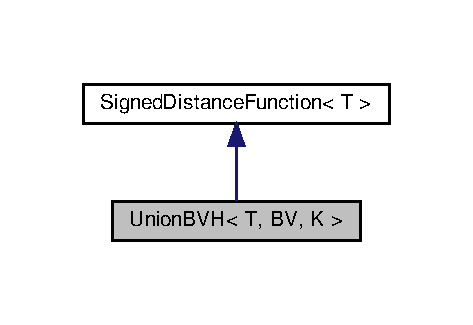
\includegraphics[width=242pt]{classUnionBVH__inherit__graph}
\end{center}
\end{figure}


Collaboration diagram for Union\+B\+VH$<$ T, BV, K $>$\+:
\nopagebreak
\begin{figure}[H]
\begin{center}
\leavevmode
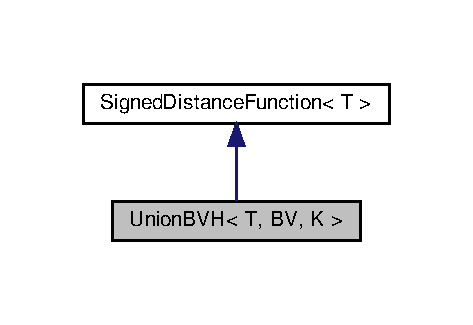
\includegraphics[width=242pt]{classUnionBVH__coll__graph}
\end{center}
\end{figure}
\doxysubsection*{Public Types}
\begin{DoxyCompactItemize}
\item 
\mbox{\Hypertarget{classUnionBVH_a5d1d64d7cabf1000fc1a804d06e103cc}\label{classUnionBVH_a5d1d64d7cabf1000fc1a804d06e103cc}} 
using \mbox{\hyperlink{classUnionBVH_a5d1d64d7cabf1000fc1a804d06e103cc}{S\+DF}} = \mbox{\hyperlink{classSignedDistanceFunction}{Signed\+Distance\+Function}}$<$ T $>$
\begin{DoxyCompactList}\small\item\em Alias for cutting down on typing. \end{DoxyCompactList}\item 
\mbox{\Hypertarget{classUnionBVH_a09561e026cd6a7da1a7dbdbad5eea2c2}\label{classUnionBVH_a09561e026cd6a7da1a7dbdbad5eea2c2}} 
using \mbox{\hyperlink{classUnionBVH_a09561e026cd6a7da1a7dbdbad5eea2c2}{B\+V\+Constructor}} = E\+B\+Geometry\+::\+B\+V\+H\+::\+B\+V\+ConstructorT$<$ \mbox{\hyperlink{classUnionBVH_a5d1d64d7cabf1000fc1a804d06e103cc}{S\+DF}}, BV $>$
\begin{DoxyCompactList}\small\item\em Alias for cutting down on typing. This is a std\+::function$<$\+B\+V(\+S\+D\+F)$>$, i.\+e. a function which returns a bounding volume for an S\+DF. \end{DoxyCompactList}\end{DoxyCompactItemize}
\doxysubsection*{Public Member Functions}
\begin{DoxyCompactItemize}
\item 
\mbox{\Hypertarget{classUnionBVH_aa2d9a2e95e58a0d7dfb2b92283626cac}\label{classUnionBVH_aa2d9a2e95e58a0d7dfb2b92283626cac}} 
\mbox{\hyperlink{classUnionBVH_aa2d9a2e95e58a0d7dfb2b92283626cac}{Union\+B\+VH}} ()=delete
\begin{DoxyCompactList}\small\item\em Disallowed, use the full constructor. \end{DoxyCompactList}\item 
\mbox{\hyperlink{classUnionBVH_ab56dd603f45f3908be3386fd295d9ffc}{Union\+B\+VH}} (const std\+::vector$<$ std\+::shared\+\_\+ptr$<$ \mbox{\hyperlink{classUnionBVH_a5d1d64d7cabf1000fc1a804d06e103cc}{S\+DF}} $>$$>$ \&a\+\_\+distance\+Functions, const bool a\+\_\+flip\+Sign)
\begin{DoxyCompactList}\small\item\em Partial constructor. Associates distance functions but does not build \mbox{\hyperlink{namespaceBVH}{B\+VH}} tree. \end{DoxyCompactList}\item 
\mbox{\hyperlink{classUnionBVH_adc951cd9eb51c029a25e33e275e74f25}{Union\+B\+VH}} (const std\+::vector$<$ std\+::shared\+\_\+ptr$<$ \mbox{\hyperlink{classUnionBVH_a5d1d64d7cabf1000fc1a804d06e103cc}{S\+DF}} $>$$>$ \&a\+\_\+distance\+Functions, const bool a\+\_\+flip\+Sign, const \mbox{\hyperlink{classUnionBVH_a09561e026cd6a7da1a7dbdbad5eea2c2}{B\+V\+Constructor}} \&a\+\_\+bv\+Constructor)
\begin{DoxyCompactList}\small\item\em Full constructor. \end{DoxyCompactList}\item 
void \mbox{\hyperlink{classUnionBVH_a97769f4c449610b681a70b93c99a40ca}{build\+Tree}} (const \mbox{\hyperlink{classUnionBVH_a09561e026cd6a7da1a7dbdbad5eea2c2}{B\+V\+Constructor}} \&a\+\_\+bv\+Constructor)
\begin{DoxyCompactList}\small\item\em Build \mbox{\hyperlink{namespaceBVH}{B\+VH}} tree for the input objects. User must supply a partitioner and a BV constructor for the S\+DF objects. \end{DoxyCompactList}\item 
\mbox{\Hypertarget{classUnionBVH_aac0a1f16ad0a273e72c8bcd15b80f336}\label{classUnionBVH_aac0a1f16ad0a273e72c8bcd15b80f336}} 
virtual \mbox{\hyperlink{classUnionBVH_aac0a1f16ad0a273e72c8bcd15b80f336}{$\sim$\+Union\+B\+VH}} ()=default
\begin{DoxyCompactList}\small\item\em Destructor (does nothing) \end{DoxyCompactList}\item 
T \mbox{\hyperlink{classUnionBVH_a9681fdc161e2e077a33caaddb78fb4ba}{signed\+Distance}} (const \mbox{\hyperlink{classVec3T}{Vec3T}}$<$ T $>$ \&a\+\_\+point) const noexcept override
\begin{DoxyCompactList}\small\item\em Value function. \end{DoxyCompactList}\end{DoxyCompactItemize}
\doxysubsection*{Protected Types}
\begin{DoxyCompactItemize}
\item 
\mbox{\Hypertarget{classUnionBVH_ac23ace50239fbe00130df2a7e42af995}\label{classUnionBVH_ac23ace50239fbe00130df2a7e42af995}} 
using \mbox{\hyperlink{classUnionBVH_ac23ace50239fbe00130df2a7e42af995}{S\+D\+F\+List}} = std\+::vector$<$ std\+::shared\+\_\+ptr$<$ const \mbox{\hyperlink{classUnionBVH_a5d1d64d7cabf1000fc1a804d06e103cc}{S\+DF}} $>$ $>$
\begin{DoxyCompactList}\small\item\em Alias for cutting down on typing. \end{DoxyCompactList}\item 
\mbox{\Hypertarget{classUnionBVH_a9fd434576440274a81c0251962d7ff7e}\label{classUnionBVH_a9fd434576440274a81c0251962d7ff7e}} 
using \mbox{\hyperlink{classUnionBVH_a9fd434576440274a81c0251962d7ff7e}{Builder\+Node}} = E\+B\+Geometry\+::\+B\+V\+H\+::\+NodeT$<$ T, \mbox{\hyperlink{classUnionBVH_a5d1d64d7cabf1000fc1a804d06e103cc}{S\+DF}}, BV, K $>$
\begin{DoxyCompactList}\small\item\em Builder node type in \mbox{\hyperlink{namespaceBVH}{B\+VH}} tree. Tree is constructed in \char`\"{}full\char`\"{}. \end{DoxyCompactList}\item 
\mbox{\Hypertarget{classUnionBVH_a25cac5a9dc5396299f06399434ebe212}\label{classUnionBVH_a25cac5a9dc5396299f06399434ebe212}} 
using \mbox{\hyperlink{classUnionBVH_a25cac5a9dc5396299f06399434ebe212}{Linear\+Node}} = E\+B\+Geometry\+::\+B\+V\+H\+::\+Linear\+B\+VH$<$ T, \mbox{\hyperlink{classUnionBVH_a5d1d64d7cabf1000fc1a804d06e103cc}{S\+DF}}, BV, K $>$
\begin{DoxyCompactList}\small\item\em Node type in \mbox{\hyperlink{namespaceBVH}{B\+VH}} tree. We use a flattened tree. \end{DoxyCompactList}\end{DoxyCompactItemize}
\doxysubsection*{Protected Attributes}
\begin{DoxyCompactItemize}
\item 
\mbox{\Hypertarget{classUnionBVH_a026a103a13d0b04bedb6dabd50e4da69}\label{classUnionBVH_a026a103a13d0b04bedb6dabd50e4da69}} 
std\+::vector$<$ std\+::shared\+\_\+ptr$<$ const \mbox{\hyperlink{classUnionBVH_a5d1d64d7cabf1000fc1a804d06e103cc}{S\+DF}} $>$ $>$ \mbox{\hyperlink{classUnionBVH_a026a103a13d0b04bedb6dabd50e4da69}{m\+\_\+distance\+Functions}}
\begin{DoxyCompactList}\small\item\em List of distance functions. \end{DoxyCompactList}\item 
\mbox{\Hypertarget{classUnionBVH_ad59be4f96e0f020c28f4677dcb94a004}\label{classUnionBVH_ad59be4f96e0f020c28f4677dcb94a004}} 
std\+::shared\+\_\+ptr$<$ \mbox{\hyperlink{classUnionBVH_a25cac5a9dc5396299f06399434ebe212}{Linear\+Node}} $>$ \mbox{\hyperlink{classUnionBVH_ad59be4f96e0f020c28f4677dcb94a004}{m\+\_\+root\+Node}}
\begin{DoxyCompactList}\small\item\em Root node for \mbox{\hyperlink{namespaceBVH}{B\+VH}} tree. \end{DoxyCompactList}\item 
\mbox{\Hypertarget{classUnionBVH_a2c3a008bd61f225a83c959f2280b9649}\label{classUnionBVH_a2c3a008bd61f225a83c959f2280b9649}} 
bool \mbox{\hyperlink{classUnionBVH_a2c3a008bd61f225a83c959f2280b9649}{m\+\_\+is\+Good}}
\begin{DoxyCompactList}\small\item\em Is good or not. \end{DoxyCompactList}\item 
\mbox{\Hypertarget{classUnionBVH_a0782d93bd0a7bff7580a99e6fef285c7}\label{classUnionBVH_a0782d93bd0a7bff7580a99e6fef285c7}} 
bool \mbox{\hyperlink{classUnionBVH_a0782d93bd0a7bff7580a99e6fef285c7}{m\+\_\+flip\+Sign}}
\begin{DoxyCompactList}\small\item\em Hook for turning inside to outside. \end{DoxyCompactList}\end{DoxyCompactItemize}
\doxysubsection*{Additional Inherited Members}


\doxysubsection{Detailed Description}
\subsubsection*{template$<$class T, class BV, size\+\_\+t K$>$\newline
class Union\+B\+V\+H$<$ T, B\+V, K $>$}

Distance function union using B\+V\+Hs. Computes the signed distance to the closest object of N non-\/overlapping objects. 

\begin{DoxyNote}{Note}
This class only makes sense if the object do not overlap. 
\end{DoxyNote}


\doxysubsection{Constructor \& Destructor Documentation}
\mbox{\Hypertarget{classUnionBVH_ab56dd603f45f3908be3386fd295d9ffc}\label{classUnionBVH_ab56dd603f45f3908be3386fd295d9ffc}} 
\index{UnionBVH$<$ T, BV, K $>$@{UnionBVH$<$ T, BV, K $>$}!UnionBVH@{UnionBVH}}
\index{UnionBVH@{UnionBVH}!UnionBVH$<$ T, BV, K $>$@{UnionBVH$<$ T, BV, K $>$}}
\doxysubsubsection{\texorpdfstring{UnionBVH()}{UnionBVH()}\hspace{0.1cm}{\footnotesize\ttfamily [1/2]}}
{\footnotesize\ttfamily template$<$class T , class BV , size\+\_\+t K$>$ \\
\mbox{\hyperlink{classUnionBVH}{Union\+B\+VH}}$<$ T, BV, K $>$\+::\mbox{\hyperlink{classUnionBVH}{Union\+B\+VH}} (\begin{DoxyParamCaption}\item[{const std\+::vector$<$ std\+::shared\+\_\+ptr$<$ \mbox{\hyperlink{classUnionBVH_a5d1d64d7cabf1000fc1a804d06e103cc}{S\+DF}} $>$$>$ \&}]{a\+\_\+distance\+Functions,  }\item[{const bool}]{a\+\_\+flip\+Sign }\end{DoxyParamCaption})}



Partial constructor. Associates distance functions but does not build \mbox{\hyperlink{namespaceBVH}{B\+VH}} tree. 


\begin{DoxyParams}[1]{Parameters}
\mbox{\texttt{ in}}  & {\em a\+\_\+distance\+Functions} & Signed distance functions. \\
\hline
\mbox{\texttt{ in}}  & {\em a\+\_\+flip\+Sign} & Hook for turning inside to outside \\
\hline
\end{DoxyParams}
\mbox{\Hypertarget{classUnionBVH_adc951cd9eb51c029a25e33e275e74f25}\label{classUnionBVH_adc951cd9eb51c029a25e33e275e74f25}} 
\index{UnionBVH$<$ T, BV, K $>$@{UnionBVH$<$ T, BV, K $>$}!UnionBVH@{UnionBVH}}
\index{UnionBVH@{UnionBVH}!UnionBVH$<$ T, BV, K $>$@{UnionBVH$<$ T, BV, K $>$}}
\doxysubsubsection{\texorpdfstring{UnionBVH()}{UnionBVH()}\hspace{0.1cm}{\footnotesize\ttfamily [2/2]}}
{\footnotesize\ttfamily template$<$class T , class BV , size\+\_\+t K$>$ \\
\mbox{\hyperlink{classUnionBVH}{Union\+B\+VH}}$<$ T, BV, K $>$\+::\mbox{\hyperlink{classUnionBVH}{Union\+B\+VH}} (\begin{DoxyParamCaption}\item[{const std\+::vector$<$ std\+::shared\+\_\+ptr$<$ \mbox{\hyperlink{classUnionBVH_a5d1d64d7cabf1000fc1a804d06e103cc}{S\+DF}} $>$$>$ \&}]{a\+\_\+distance\+Functions,  }\item[{const bool}]{a\+\_\+flip\+Sign,  }\item[{const \mbox{\hyperlink{classUnionBVH_a09561e026cd6a7da1a7dbdbad5eea2c2}{B\+V\+Constructor}} \&}]{a\+\_\+bv\+Constructor }\end{DoxyParamCaption})}



Full constructor. 


\begin{DoxyParams}[1]{Parameters}
\mbox{\texttt{ in}}  & {\em a\+\_\+distance\+Functions} & Signed distance functions. \\
\hline
\mbox{\texttt{ in}}  & {\em a\+\_\+flip\+Sign} & Hook for turning inside to outside \\
\hline
\mbox{\texttt{ in}}  & {\em a\+\_\+bv\+Constructor} & Bounding volume constructor. \\
\hline
\end{DoxyParams}


\doxysubsection{Member Function Documentation}
\mbox{\Hypertarget{classUnionBVH_a97769f4c449610b681a70b93c99a40ca}\label{classUnionBVH_a97769f4c449610b681a70b93c99a40ca}} 
\index{UnionBVH$<$ T, BV, K $>$@{UnionBVH$<$ T, BV, K $>$}!buildTree@{buildTree}}
\index{buildTree@{buildTree}!UnionBVH$<$ T, BV, K $>$@{UnionBVH$<$ T, BV, K $>$}}
\doxysubsubsection{\texorpdfstring{buildTree()}{buildTree()}}
{\footnotesize\ttfamily template$<$class T , class BV , size\+\_\+t K$>$ \\
void \mbox{\hyperlink{classUnionBVH}{Union\+B\+VH}}$<$ T, BV, K $>$\+::build\+Tree (\begin{DoxyParamCaption}\item[{const \mbox{\hyperlink{classUnionBVH_a09561e026cd6a7da1a7dbdbad5eea2c2}{B\+V\+Constructor}} \&}]{a\+\_\+bv\+Constructor }\end{DoxyParamCaption})}



Build \mbox{\hyperlink{namespaceBVH}{B\+VH}} tree for the input objects. User must supply a partitioner and a BV constructor for the S\+DF objects. 


\begin{DoxyParams}[1]{Parameters}
\mbox{\texttt{ in}}  & {\em a\+\_\+bv\+Constructor} & Constructor for building a bounding volume that encloses an object. \\
\hline
\end{DoxyParams}
\mbox{\Hypertarget{classUnionBVH_a9681fdc161e2e077a33caaddb78fb4ba}\label{classUnionBVH_a9681fdc161e2e077a33caaddb78fb4ba}} 
\index{UnionBVH$<$ T, BV, K $>$@{UnionBVH$<$ T, BV, K $>$}!signedDistance@{signedDistance}}
\index{signedDistance@{signedDistance}!UnionBVH$<$ T, BV, K $>$@{UnionBVH$<$ T, BV, K $>$}}
\doxysubsubsection{\texorpdfstring{signedDistance()}{signedDistance()}}
{\footnotesize\ttfamily template$<$class T , class BV , size\+\_\+t K$>$ \\
T \mbox{\hyperlink{classUnionBVH}{Union\+B\+VH}}$<$ T, BV, K $>$\+::signed\+Distance (\begin{DoxyParamCaption}\item[{const \mbox{\hyperlink{classVec3T}{Vec3T}}$<$ T $>$ \&}]{a\+\_\+point }\end{DoxyParamCaption}) const\hspace{0.3cm}{\ttfamily [override]}, {\ttfamily [virtual]}, {\ttfamily [noexcept]}}



Value function. 


\begin{DoxyParams}[1]{Parameters}
\mbox{\texttt{ in}}  & {\em a\+\_\+point} & 3D point. \\
\hline
\end{DoxyParams}


Implements \mbox{\hyperlink{classSignedDistanceFunction_af5912280ca51dc21a2d6949a30ec7d21}{Signed\+Distance\+Function$<$ T $>$}}.



The documentation for this class was generated from the following files\+:\begin{DoxyCompactItemize}
\item 
Source/\mbox{\hyperlink{EBGeometry__UnionBVH_8hpp}{E\+B\+Geometry\+\_\+\+Union\+B\+V\+H.\+hpp}}\item 
Source/\mbox{\hyperlink{EBGeometry__UnionBVHImplem_8hpp}{E\+B\+Geometry\+\_\+\+Union\+B\+V\+H\+Implem.\+hpp}}\end{DoxyCompactItemize}

\hypertarget{classVec2T}{}\doxysection{Vec2T$<$ T $>$ Class Template Reference}
\label{classVec2T}\index{Vec2T$<$ T $>$@{Vec2T$<$ T $>$}}


Two-\/dimensional vector class with arithmetic operators.  




{\ttfamily \#include $<$EBGeometry\+\_\+\+Vec.\+hpp$>$}

\doxysubsection*{Public Member Functions}
\begin{DoxyCompactItemize}
\item 
\mbox{\Hypertarget{classVec2T_a4aa6e0bd3922abd84449278429a03418}\label{classVec2T_a4aa6e0bd3922abd84449278429a03418}} 
\mbox{\hyperlink{classVec2T_a4aa6e0bd3922abd84449278429a03418}{Vec2T}} ()
\begin{DoxyCompactList}\small\item\em Default constructor. Sets the vector to the zero vector. \end{DoxyCompactList}\item 
\mbox{\hyperlink{classVec2T_ae58412c19542cb4c76553e53e74a1203}{Vec2T}} (const \mbox{\hyperlink{classVec2T}{Vec2T}} \&u) noexcept
\begin{DoxyCompactList}\small\item\em Copy constructor. \end{DoxyCompactList}\item 
constexpr \mbox{\hyperlink{classVec2T_a6ab40f6698f98b18934ff65046277540}{Vec2T}} (const T \&a\+\_\+x, const T \&a\+\_\+y)
\begin{DoxyCompactList}\small\item\em Full constructor. \end{DoxyCompactList}\item 
\mbox{\Hypertarget{classVec2T_a15a9bac13b94b58f0907443bc551dbee}\label{classVec2T_a15a9bac13b94b58f0907443bc551dbee}} 
\mbox{\hyperlink{classVec2T_a15a9bac13b94b58f0907443bc551dbee}{$\sim$\+Vec2T}} ()=default
\begin{DoxyCompactList}\small\item\em Destructor (does nothing) \end{DoxyCompactList}\item 
constexpr \mbox{\hyperlink{classVec2T}{Vec2T}}$<$ T $>$ \& \mbox{\hyperlink{classVec2T_adb211f83d3075c8e90bc7bd2367f0595}{operator=}} (const \mbox{\hyperlink{classVec2T}{Vec2T}} \&a\+\_\+other) noexcept
\begin{DoxyCompactList}\small\item\em Assignment operator. Sets this.\+x = a\+\_\+other.\+x and this.\+y = a\+\_\+other.\+y. \end{DoxyCompactList}\item 
constexpr \mbox{\hyperlink{classVec2T}{Vec2T}}$<$ T $>$ \mbox{\hyperlink{classVec2T_a8ea575fe13a084e34b52d4a41f280c0e}{operator+}} (const \mbox{\hyperlink{classVec2T}{Vec2T}} \&a\+\_\+other) const noexcept
\begin{DoxyCompactList}\small\item\em Addition operator. \end{DoxyCompactList}\item 
constexpr \mbox{\hyperlink{classVec2T}{Vec2T}}$<$ T $>$ \mbox{\hyperlink{classVec2T_a99adc1e31339edeb7972cb4dee35ff79}{operator-\/}} (const \mbox{\hyperlink{classVec2T}{Vec2T}} \&a\+\_\+other) const noexcept
\begin{DoxyCompactList}\small\item\em Subtraction operator. \end{DoxyCompactList}\item 
\mbox{\Hypertarget{classVec2T_aaf91f8ec851e9757665de800e8d54b1e}\label{classVec2T_aaf91f8ec851e9757665de800e8d54b1e}} 
constexpr \mbox{\hyperlink{classVec2T}{Vec2T}}$<$ T $>$ \mbox{\hyperlink{classVec2T_aaf91f8ec851e9757665de800e8d54b1e}{operator-\/}} () const noexcept
\begin{DoxyCompactList}\small\item\em Negation operator. Returns a new Vec2\+T$<$\+T$>$ with negated components. \end{DoxyCompactList}\item 
constexpr \mbox{\hyperlink{classVec2T}{Vec2T}}$<$ T $>$ \mbox{\hyperlink{classVec2T_a0d4c29c9de8965647f7ddf18a6df2b7f}{operator$\ast$}} (const T \&s) const noexcept
\begin{DoxyCompactList}\small\item\em Multiplication operator. \end{DoxyCompactList}\item 
constexpr \mbox{\hyperlink{classVec2T}{Vec2T}}$<$ T $>$ \mbox{\hyperlink{classVec2T_a670dafb9e1cc73148839bb78655b3392}{operator/}} (const T \&s) const noexcept
\begin{DoxyCompactList}\small\item\em Division operator. \end{DoxyCompactList}\item 
constexpr \mbox{\hyperlink{classVec2T}{Vec2T}}$<$ T $>$ \& \mbox{\hyperlink{classVec2T_a0f4161352341bef3c90c4c08c0bbb713}{operator+=}} (const \mbox{\hyperlink{classVec2T}{Vec2T}} \&a\+\_\+other) noexcept
\begin{DoxyCompactList}\small\item\em Addition operator. \end{DoxyCompactList}\item 
constexpr \mbox{\hyperlink{classVec2T}{Vec2T}}$<$ T $>$ \& \mbox{\hyperlink{classVec2T_ace969c60a66c09ccf0efafc3447c3e27}{operator-\/=}} (const \mbox{\hyperlink{classVec2T}{Vec2T}} \&a\+\_\+other) noexcept
\begin{DoxyCompactList}\small\item\em Subtraction operator. \end{DoxyCompactList}\item 
constexpr \mbox{\hyperlink{classVec2T}{Vec2T}}$<$ T $>$ \& \mbox{\hyperlink{classVec2T_ad0f92374027e7fc6288c8f4d524dfec8}{operator$\ast$=}} (const T \&s) noexcept
\begin{DoxyCompactList}\small\item\em Multiplication operator. \end{DoxyCompactList}\item 
constexpr \mbox{\hyperlink{classVec2T}{Vec2T}}$<$ T $>$ \& \mbox{\hyperlink{classVec2T_ae28b03fbebd9cdb961af47fc447a7f9e}{operator/=}} (const T \&s) noexcept
\begin{DoxyCompactList}\small\item\em Division operator operator. \end{DoxyCompactList}\item 
constexpr T \mbox{\hyperlink{classVec2T_a8b7cb7e36ad7739929bcebdbce3a30de}{dot}} (const \mbox{\hyperlink{classVec2T}{Vec2T}} \&a\+\_\+other) const noexcept
\begin{DoxyCompactList}\small\item\em Dot product operator. \end{DoxyCompactList}\item 
constexpr T \mbox{\hyperlink{classVec2T_a006955e162c59d5d4988032be46b173c}{length}} () const noexcept
\begin{DoxyCompactList}\small\item\em Compute length of vector. \end{DoxyCompactList}\item 
constexpr T \mbox{\hyperlink{classVec2T_a29e28df03549a51e58e25bee8ef92b23}{length2}} () const noexcept
\begin{DoxyCompactList}\small\item\em Compute square of vector. \end{DoxyCompactList}\end{DoxyCompactItemize}
\doxysubsection*{Static Public Member Functions}
\begin{DoxyCompactItemize}
\item 
\mbox{\Hypertarget{classVec2T_a55c716414b5db6d83d736b0e5a2363b9}\label{classVec2T_a55c716414b5db6d83d736b0e5a2363b9}} 
static constexpr \mbox{\hyperlink{classVec2T}{Vec2T}}$<$ T $>$ \mbox{\hyperlink{classVec2T_a55c716414b5db6d83d736b0e5a2363b9}{zero}} () noexcept
\begin{DoxyCompactList}\small\item\em Return av vector with x = y = 0. \end{DoxyCompactList}\item 
\mbox{\Hypertarget{classVec2T_ac5c9ebc02a898817386d3114d5d88da0}\label{classVec2T_ac5c9ebc02a898817386d3114d5d88da0}} 
static constexpr \mbox{\hyperlink{classVec2T}{Vec2T}}$<$ T $>$ \mbox{\hyperlink{classVec2T_ac5c9ebc02a898817386d3114d5d88da0}{one}} () noexcept
\begin{DoxyCompactList}\small\item\em Return av vector with x = y = 1. \end{DoxyCompactList}\item 
\mbox{\Hypertarget{classVec2T_a8683604bcdccc2e4d0b04bb473ace422}\label{classVec2T_a8683604bcdccc2e4d0b04bb473ace422}} 
static constexpr \mbox{\hyperlink{classVec2T}{Vec2T}}$<$ T $>$ \mbox{\hyperlink{classVec2T_a8683604bcdccc2e4d0b04bb473ace422}{min}} () noexcept
\begin{DoxyCompactList}\small\item\em Return minimum possible representative vector. \end{DoxyCompactList}\item 
\mbox{\Hypertarget{classVec2T_a3d59b621d38a154f108c01cdd153a1ef}\label{classVec2T_a3d59b621d38a154f108c01cdd153a1ef}} 
static constexpr \mbox{\hyperlink{classVec2T}{Vec2T}}$<$ T $>$ \mbox{\hyperlink{classVec2T_a3d59b621d38a154f108c01cdd153a1ef}{max}} () noexcept
\begin{DoxyCompactList}\small\item\em Return maximum possible representative vector. \end{DoxyCompactList}\item 
\mbox{\Hypertarget{classVec2T_aae152c05bb2b8912703076f0c811ab82}\label{classVec2T_aae152c05bb2b8912703076f0c811ab82}} 
static constexpr \mbox{\hyperlink{classVec2T}{Vec2T}}$<$ T $>$ \mbox{\hyperlink{classVec2T_aae152c05bb2b8912703076f0c811ab82}{infinity}} () noexcept
\begin{DoxyCompactList}\small\item\em Return a vector with inf components. \end{DoxyCompactList}\end{DoxyCompactItemize}
\doxysubsection*{Public Attributes}
\begin{DoxyCompactItemize}
\item 
\mbox{\Hypertarget{classVec2T_a66ea295b52114b22de1f76cce1aa7f51}\label{classVec2T_a66ea295b52114b22de1f76cce1aa7f51}} 
T \mbox{\hyperlink{classVec2T_a66ea295b52114b22de1f76cce1aa7f51}{x}}
\begin{DoxyCompactList}\small\item\em First component in the vector. \end{DoxyCompactList}\item 
\mbox{\Hypertarget{classVec2T_a71ce5251d618a6dbd4e0e7a0f867b6cf}\label{classVec2T_a71ce5251d618a6dbd4e0e7a0f867b6cf}} 
T \mbox{\hyperlink{classVec2T_a71ce5251d618a6dbd4e0e7a0f867b6cf}{y}}
\begin{DoxyCompactList}\small\item\em Second component in the vector. \end{DoxyCompactList}\end{DoxyCompactItemize}


\doxysubsection{Detailed Description}
\subsubsection*{template$<$typename T$>$\newline
class Vec2\+T$<$ T $>$}

Two-\/dimensional vector class with arithmetic operators. 

The class has a public-\/only interface. To change it\textquotesingle{}s components one can call the member functions, or set components directly, e.\+g. vec.\+x = 5.\+0 \begin{DoxyNote}{Note}
\mbox{\hyperlink{classVec2T}{Vec2T}} is a templated class primarily used with \mbox{\hyperlink{namespaceDCEL}{DCEL}} grids. 
\end{DoxyNote}


\doxysubsection{Constructor \& Destructor Documentation}
\mbox{\Hypertarget{classVec2T_ae58412c19542cb4c76553e53e74a1203}\label{classVec2T_ae58412c19542cb4c76553e53e74a1203}} 
\index{Vec2T$<$ T $>$@{Vec2T$<$ T $>$}!Vec2T@{Vec2T}}
\index{Vec2T@{Vec2T}!Vec2T$<$ T $>$@{Vec2T$<$ T $>$}}
\doxysubsubsection{\texorpdfstring{Vec2T()}{Vec2T()}\hspace{0.1cm}{\footnotesize\ttfamily [1/2]}}
{\footnotesize\ttfamily template$<$typename T $>$ \\
\mbox{\hyperlink{classVec2T}{Vec2T}}$<$ T $>$\+::\mbox{\hyperlink{classVec2T}{Vec2T}} (\begin{DoxyParamCaption}\item[{const \mbox{\hyperlink{classVec2T}{Vec2T}}$<$ T $>$ \&}]{u }\end{DoxyParamCaption})\hspace{0.3cm}{\ttfamily [noexcept]}}



Copy constructor. 


\begin{DoxyParams}[1]{Parameters}
\mbox{\texttt{ in}}  & {\em u} & Other vector\\
\hline
\end{DoxyParams}
Sets $\ast$this = u \mbox{\Hypertarget{classVec2T_a6ab40f6698f98b18934ff65046277540}\label{classVec2T_a6ab40f6698f98b18934ff65046277540}} 
\index{Vec2T$<$ T $>$@{Vec2T$<$ T $>$}!Vec2T@{Vec2T}}
\index{Vec2T@{Vec2T}!Vec2T$<$ T $>$@{Vec2T$<$ T $>$}}
\doxysubsubsection{\texorpdfstring{Vec2T()}{Vec2T()}\hspace{0.1cm}{\footnotesize\ttfamily [2/2]}}
{\footnotesize\ttfamily template$<$typename T $>$ \\
constexpr \mbox{\hyperlink{classVec2T}{Vec2T}}$<$ T $>$\+::\mbox{\hyperlink{classVec2T}{Vec2T}} (\begin{DoxyParamCaption}\item[{const T \&}]{a\+\_\+x,  }\item[{const T \&}]{a\+\_\+y }\end{DoxyParamCaption})\hspace{0.3cm}{\ttfamily [constexpr]}}



Full constructor. 


\begin{DoxyParams}[1]{Parameters}
\mbox{\texttt{ in}}  & {\em a\+\_\+x} & First vector component \\
\hline
\mbox{\texttt{ in}}  & {\em a\+\_\+y} & Second vector component\\
\hline
\end{DoxyParams}
Sets this-\/$>$x = a\+\_\+x and this-\/$>$y = a\+\_\+y 

\doxysubsection{Member Function Documentation}
\mbox{\Hypertarget{classVec2T_a8b7cb7e36ad7739929bcebdbce3a30de}\label{classVec2T_a8b7cb7e36ad7739929bcebdbce3a30de}} 
\index{Vec2T$<$ T $>$@{Vec2T$<$ T $>$}!dot@{dot}}
\index{dot@{dot}!Vec2T$<$ T $>$@{Vec2T$<$ T $>$}}
\doxysubsubsection{\texorpdfstring{dot()}{dot()}}
{\footnotesize\ttfamily template$<$typename T $>$ \\
constexpr T \mbox{\hyperlink{classVec2T}{Vec2T}}$<$ T $>$\+::dot (\begin{DoxyParamCaption}\item[{const \mbox{\hyperlink{classVec2T}{Vec2T}}$<$ T $>$ \&}]{a\+\_\+other }\end{DoxyParamCaption}) const\hspace{0.3cm}{\ttfamily [inline]}, {\ttfamily [constexpr]}, {\ttfamily [noexcept]}}



Dot product operator. 


\begin{DoxyParams}[1]{Parameters}
\mbox{\texttt{ in}}  & {\em a\+\_\+other} & other vector\\
\hline
\end{DoxyParams}
Returns the dot product, i.\+e. this-\/$>$x$\ast$a\+\_\+other.x + this-\/$>$y+a\+\_\+other.y \mbox{\Hypertarget{classVec2T_a006955e162c59d5d4988032be46b173c}\label{classVec2T_a006955e162c59d5d4988032be46b173c}} 
\index{Vec2T$<$ T $>$@{Vec2T$<$ T $>$}!length@{length}}
\index{length@{length}!Vec2T$<$ T $>$@{Vec2T$<$ T $>$}}
\doxysubsubsection{\texorpdfstring{length()}{length()}}
{\footnotesize\ttfamily template$<$typename T $>$ \\
constexpr T \mbox{\hyperlink{classVec2T}{Vec2T}}$<$ T $>$\+::length (\begin{DoxyParamCaption}{ }\end{DoxyParamCaption}) const\hspace{0.3cm}{\ttfamily [inline]}, {\ttfamily [constexpr]}, {\ttfamily [noexcept]}}



Compute length of vector. 

\begin{DoxyReturn}{Returns}
Returns length of vector, i.\+e. sqrt\mbox{[}(this-\/$>$x)$\ast$(this-\/$>$x) + (this-\/$>$y)$\ast$(this-\/$>$y)\mbox{]} 
\end{DoxyReturn}
\mbox{\Hypertarget{classVec2T_a29e28df03549a51e58e25bee8ef92b23}\label{classVec2T_a29e28df03549a51e58e25bee8ef92b23}} 
\index{Vec2T$<$ T $>$@{Vec2T$<$ T $>$}!length2@{length2}}
\index{length2@{length2}!Vec2T$<$ T $>$@{Vec2T$<$ T $>$}}
\doxysubsubsection{\texorpdfstring{length2()}{length2()}}
{\footnotesize\ttfamily template$<$typename T $>$ \\
constexpr T \mbox{\hyperlink{classVec2T}{Vec2T}}$<$ T $>$\+::length2 (\begin{DoxyParamCaption}{ }\end{DoxyParamCaption}) const\hspace{0.3cm}{\ttfamily [inline]}, {\ttfamily [constexpr]}, {\ttfamily [noexcept]}}



Compute square of vector. 

\begin{DoxyReturn}{Returns}
Returns length of vector, i.\+e. (this-\/$>$x)$\ast$(this-\/$>$x) + (this-\/$>$y)$\ast$(this-\/$>$y) 
\end{DoxyReturn}
\mbox{\Hypertarget{classVec2T_a0d4c29c9de8965647f7ddf18a6df2b7f}\label{classVec2T_a0d4c29c9de8965647f7ddf18a6df2b7f}} 
\index{Vec2T$<$ T $>$@{Vec2T$<$ T $>$}!operator$\ast$@{operator$\ast$}}
\index{operator$\ast$@{operator$\ast$}!Vec2T$<$ T $>$@{Vec2T$<$ T $>$}}
\doxysubsubsection{\texorpdfstring{operator$\ast$()}{operator*()}}
{\footnotesize\ttfamily template$<$typename T $>$ \\
constexpr \mbox{\hyperlink{classVec2T}{Vec2T}}$<$T$>$ \mbox{\hyperlink{classVec2T}{Vec2T}}$<$ T $>$\+::operator$\ast$ (\begin{DoxyParamCaption}\item[{const T \&}]{s }\end{DoxyParamCaption}) const\hspace{0.3cm}{\ttfamily [inline]}, {\ttfamily [constexpr]}, {\ttfamily [noexcept]}}



Multiplication operator. 


\begin{DoxyParams}[1]{Parameters}
\mbox{\texttt{ in}}  & {\em s} & Scalar to be multiplied\\
\hline
\end{DoxyParams}
Returns a new Vec2\+T$<$\+T$>$ with components x = s$\ast$this-\/$>$x (and same for y) \mbox{\Hypertarget{classVec2T_ad0f92374027e7fc6288c8f4d524dfec8}\label{classVec2T_ad0f92374027e7fc6288c8f4d524dfec8}} 
\index{Vec2T$<$ T $>$@{Vec2T$<$ T $>$}!operator$\ast$=@{operator$\ast$=}}
\index{operator$\ast$=@{operator$\ast$=}!Vec2T$<$ T $>$@{Vec2T$<$ T $>$}}
\doxysubsubsection{\texorpdfstring{operator$\ast$=()}{operator*=()}}
{\footnotesize\ttfamily template$<$typename T $>$ \\
constexpr \mbox{\hyperlink{classVec2T}{Vec2T}}$<$T$>$\& \mbox{\hyperlink{classVec2T}{Vec2T}}$<$ T $>$\+::operator$\ast$= (\begin{DoxyParamCaption}\item[{const T \&}]{s }\end{DoxyParamCaption})\hspace{0.3cm}{\ttfamily [inline]}, {\ttfamily [constexpr]}, {\ttfamily [noexcept]}}



Multiplication operator. 


\begin{DoxyParams}[1]{Parameters}
\mbox{\texttt{ in}}  & {\em s} & Scalar to multiply by\\
\hline
\end{DoxyParams}
Returns ($\ast$this) with components this-\/$>$x = s$\ast$this-\/$>$x (and same for y) \mbox{\Hypertarget{classVec2T_a8ea575fe13a084e34b52d4a41f280c0e}\label{classVec2T_a8ea575fe13a084e34b52d4a41f280c0e}} 
\index{Vec2T$<$ T $>$@{Vec2T$<$ T $>$}!operator+@{operator+}}
\index{operator+@{operator+}!Vec2T$<$ T $>$@{Vec2T$<$ T $>$}}
\doxysubsubsection{\texorpdfstring{operator+()}{operator+()}}
{\footnotesize\ttfamily template$<$typename T $>$ \\
constexpr \mbox{\hyperlink{classVec2T}{Vec2T}}$<$T$>$ \mbox{\hyperlink{classVec2T}{Vec2T}}$<$ T $>$\+::operator+ (\begin{DoxyParamCaption}\item[{const \mbox{\hyperlink{classVec2T}{Vec2T}}$<$ T $>$ \&}]{a\+\_\+other }\end{DoxyParamCaption}) const\hspace{0.3cm}{\ttfamily [inline]}, {\ttfamily [constexpr]}, {\ttfamily [noexcept]}}



Addition operator. 


\begin{DoxyParams}[1]{Parameters}
\mbox{\texttt{ in}}  & {\em a\+\_\+other} & Other vector\\
\hline
\end{DoxyParams}
Returns a new object with component x = this-\/$>$x + a\+\_\+other.\+x (same for y-\/component) \mbox{\Hypertarget{classVec2T_a0f4161352341bef3c90c4c08c0bbb713}\label{classVec2T_a0f4161352341bef3c90c4c08c0bbb713}} 
\index{Vec2T$<$ T $>$@{Vec2T$<$ T $>$}!operator+=@{operator+=}}
\index{operator+=@{operator+=}!Vec2T$<$ T $>$@{Vec2T$<$ T $>$}}
\doxysubsubsection{\texorpdfstring{operator+=()}{operator+=()}}
{\footnotesize\ttfamily template$<$typename T $>$ \\
constexpr \mbox{\hyperlink{classVec2T}{Vec2T}}$<$T$>$\& \mbox{\hyperlink{classVec2T}{Vec2T}}$<$ T $>$\+::operator+= (\begin{DoxyParamCaption}\item[{const \mbox{\hyperlink{classVec2T}{Vec2T}}$<$ T $>$ \&}]{a\+\_\+other }\end{DoxyParamCaption})\hspace{0.3cm}{\ttfamily [inline]}, {\ttfamily [constexpr]}, {\ttfamily [noexcept]}}



Addition operator. 


\begin{DoxyParams}[1]{Parameters}
\mbox{\texttt{ in}}  & {\em a\+\_\+other} & Other vector to add\\
\hline
\end{DoxyParams}
Returns ($\ast$this) with components this-\/$>$x = this-\/$>$x + a\+\_\+other.\+x (and same for y) \mbox{\Hypertarget{classVec2T_a99adc1e31339edeb7972cb4dee35ff79}\label{classVec2T_a99adc1e31339edeb7972cb4dee35ff79}} 
\index{Vec2T$<$ T $>$@{Vec2T$<$ T $>$}!operator-\/@{operator-\/}}
\index{operator-\/@{operator-\/}!Vec2T$<$ T $>$@{Vec2T$<$ T $>$}}
\doxysubsubsection{\texorpdfstring{operator-\/()}{operator-()}}
{\footnotesize\ttfamily template$<$typename T $>$ \\
constexpr \mbox{\hyperlink{classVec2T}{Vec2T}}$<$T$>$ \mbox{\hyperlink{classVec2T}{Vec2T}}$<$ T $>$\+::operator-\/ (\begin{DoxyParamCaption}\item[{const \mbox{\hyperlink{classVec2T}{Vec2T}}$<$ T $>$ \&}]{a\+\_\+other }\end{DoxyParamCaption}) const\hspace{0.3cm}{\ttfamily [inline]}, {\ttfamily [constexpr]}, {\ttfamily [noexcept]}}



Subtraction operator. 


\begin{DoxyParams}[1]{Parameters}
\mbox{\texttt{ in}}  & {\em a\+\_\+other} & Other vector\\
\hline
\end{DoxyParams}
Returns a new object with component x = this-\/$>$x -\/ a\+\_\+other.\+x (same for y-\/component) \mbox{\Hypertarget{classVec2T_ace969c60a66c09ccf0efafc3447c3e27}\label{classVec2T_ace969c60a66c09ccf0efafc3447c3e27}} 
\index{Vec2T$<$ T $>$@{Vec2T$<$ T $>$}!operator-\/=@{operator-\/=}}
\index{operator-\/=@{operator-\/=}!Vec2T$<$ T $>$@{Vec2T$<$ T $>$}}
\doxysubsubsection{\texorpdfstring{operator-\/=()}{operator-=()}}
{\footnotesize\ttfamily template$<$typename T $>$ \\
constexpr \mbox{\hyperlink{classVec2T}{Vec2T}}$<$T$>$\& \mbox{\hyperlink{classVec2T}{Vec2T}}$<$ T $>$\+::operator-\/= (\begin{DoxyParamCaption}\item[{const \mbox{\hyperlink{classVec2T}{Vec2T}}$<$ T $>$ \&}]{a\+\_\+other }\end{DoxyParamCaption})\hspace{0.3cm}{\ttfamily [inline]}, {\ttfamily [constexpr]}, {\ttfamily [noexcept]}}



Subtraction operator. 


\begin{DoxyParams}[1]{Parameters}
\mbox{\texttt{ in}}  & {\em a\+\_\+other} & Other vector to subtract\\
\hline
\end{DoxyParams}
Returns ($\ast$this) with components this-\/$>$x = this-\/$>$x -\/ a\+\_\+other.\+x (and same for y) \mbox{\Hypertarget{classVec2T_a670dafb9e1cc73148839bb78655b3392}\label{classVec2T_a670dafb9e1cc73148839bb78655b3392}} 
\index{Vec2T$<$ T $>$@{Vec2T$<$ T $>$}!operator/@{operator/}}
\index{operator/@{operator/}!Vec2T$<$ T $>$@{Vec2T$<$ T $>$}}
\doxysubsubsection{\texorpdfstring{operator/()}{operator/()}}
{\footnotesize\ttfamily template$<$typename T $>$ \\
constexpr \mbox{\hyperlink{classVec2T}{Vec2T}}$<$T$>$ \mbox{\hyperlink{classVec2T}{Vec2T}}$<$ T $>$\+::operator/ (\begin{DoxyParamCaption}\item[{const T \&}]{s }\end{DoxyParamCaption}) const\hspace{0.3cm}{\ttfamily [inline]}, {\ttfamily [constexpr]}, {\ttfamily [noexcept]}}



Division operator. 


\begin{DoxyParams}[1]{Parameters}
\mbox{\texttt{ in}}  & {\em s} & Scalar to be multiplied\\
\hline
\end{DoxyParams}
Returns a new Vec2\+T$<$\+T$>$ with components x = (1/s)$\ast$this-\/$>$x (and same for y) \mbox{\Hypertarget{classVec2T_ae28b03fbebd9cdb961af47fc447a7f9e}\label{classVec2T_ae28b03fbebd9cdb961af47fc447a7f9e}} 
\index{Vec2T$<$ T $>$@{Vec2T$<$ T $>$}!operator/=@{operator/=}}
\index{operator/=@{operator/=}!Vec2T$<$ T $>$@{Vec2T$<$ T $>$}}
\doxysubsubsection{\texorpdfstring{operator/=()}{operator/=()}}
{\footnotesize\ttfamily template$<$typename T $>$ \\
constexpr \mbox{\hyperlink{classVec2T}{Vec2T}}$<$T$>$\& \mbox{\hyperlink{classVec2T}{Vec2T}}$<$ T $>$\+::operator/= (\begin{DoxyParamCaption}\item[{const T \&}]{s }\end{DoxyParamCaption})\hspace{0.3cm}{\ttfamily [inline]}, {\ttfamily [constexpr]}, {\ttfamily [noexcept]}}



Division operator operator. 


\begin{DoxyParams}[1]{Parameters}
\mbox{\texttt{ in}}  & {\em s} & Scalar to divide by\\
\hline
\end{DoxyParams}
Returns ($\ast$this) with components this-\/$>$x = (1/s)$\ast$this-\/$>$x (and same for y) \mbox{\Hypertarget{classVec2T_adb211f83d3075c8e90bc7bd2367f0595}\label{classVec2T_adb211f83d3075c8e90bc7bd2367f0595}} 
\index{Vec2T$<$ T $>$@{Vec2T$<$ T $>$}!operator=@{operator=}}
\index{operator=@{operator=}!Vec2T$<$ T $>$@{Vec2T$<$ T $>$}}
\doxysubsubsection{\texorpdfstring{operator=()}{operator=()}}
{\footnotesize\ttfamily template$<$typename T $>$ \\
constexpr \mbox{\hyperlink{classVec2T}{Vec2T}}$<$T$>$\& \mbox{\hyperlink{classVec2T}{Vec2T}}$<$ T $>$\+::operator= (\begin{DoxyParamCaption}\item[{const \mbox{\hyperlink{classVec2T}{Vec2T}}$<$ T $>$ \&}]{a\+\_\+other }\end{DoxyParamCaption})\hspace{0.3cm}{\ttfamily [inline]}, {\ttfamily [constexpr]}, {\ttfamily [noexcept]}}



Assignment operator. Sets this.\+x = a\+\_\+other.\+x and this.\+y = a\+\_\+other.\+y. 


\begin{DoxyParams}[1]{Parameters}
\mbox{\texttt{ in}}  & {\em a\+\_\+other} & Other vector \\
\hline
\end{DoxyParams}


The documentation for this class was generated from the following file\+:\begin{DoxyCompactItemize}
\item 
/home/runner/work/\+EBGeometry/\+EBGeometry/\+Source/\mbox{\hyperlink{EBGeometry__Vec_8hpp}{EBGeometry\+\_\+\+Vec.\+hpp}}\end{DoxyCompactItemize}

\hypertarget{classVec3T}{}\doxysection{Vec3T$<$ T $>$ Class Template Reference}
\label{classVec3T}\index{Vec3T$<$ T $>$@{Vec3T$<$ T $>$}}


Three-\/dimensional vector class with arithmetic operators.  




{\ttfamily \#include $<$E\+B\+Geometry\+\_\+\+Vec.\+hpp$>$}

\doxysubsection*{Public Member Functions}
\begin{DoxyCompactItemize}
\item 
\mbox{\Hypertarget{classVec3T_a919b1cabc678f8d71763e03fab500334}\label{classVec3T_a919b1cabc678f8d71763e03fab500334}} 
\mbox{\hyperlink{classVec3T_a919b1cabc678f8d71763e03fab500334}{Vec3T}} ()
\begin{DoxyCompactList}\small\item\em Default constructor. Sets the vector to the zero vector. \end{DoxyCompactList}\item 
\mbox{\hyperlink{classVec3T_a46379e3e007bcf0374b2d6578b6c6d71}{Vec3T}} (const \mbox{\hyperlink{classVec3T}{Vec3T}}$<$ T $>$ \&a\+\_\+u) noexcept
\begin{DoxyCompactList}\small\item\em Copy constructor. \end{DoxyCompactList}\item 
\mbox{\hyperlink{classVec3T_acc3573bc8c3232eb14a22ca833cbce30}{Vec3T}} (const T \&a\+\_\+x, const T \&a\+\_\+y, const T \&a\+\_\+z)
\begin{DoxyCompactList}\small\item\em Full constructor. \end{DoxyCompactList}\item 
\mbox{\Hypertarget{classVec3T_a505fc5de8e213d1fc8e0df5f3b7a3dc7}\label{classVec3T_a505fc5de8e213d1fc8e0df5f3b7a3dc7}} 
\mbox{\hyperlink{classVec3T_a505fc5de8e213d1fc8e0df5f3b7a3dc7}{$\sim$\+Vec3T}} ()=default
\begin{DoxyCompactList}\small\item\em Destructor (does nothing) \end{DoxyCompactList}\item 
T \& \mbox{\hyperlink{classVec3T_a76d9ddf4dc672b6867f4d1c3b7d673f2}{operator\mbox{[}$\,$\mbox{]}}} (size\+\_\+t i) noexcept
\begin{DoxyCompactList}\small\item\em Return component in vector. (i=0 =$>$ x and so on) \end{DoxyCompactList}\item 
const T \& \mbox{\hyperlink{classVec3T_adf2979413ef41584b90dc8778587a4cd}{operator\mbox{[}$\,$\mbox{]}}} (size\+\_\+t i) const noexcept
\begin{DoxyCompactList}\small\item\em Return non-\/modifiable component in vector. (i=0 =$>$ x and so on) \end{DoxyCompactList}\item 
bool \mbox{\hyperlink{classVec3T_a715546682c26647643148a80087c4ab4}{operator==}} (const \mbox{\hyperlink{classVec3T}{Vec3T}}$<$ T $>$ \&u) const noexcept
\begin{DoxyCompactList}\small\item\em Comparison operator. Returns true if all components are the same. \end{DoxyCompactList}\item 
bool \mbox{\hyperlink{classVec3T_aba830919c5020bb060f39fe9df6b7ca1}{operator$<$}} (const \mbox{\hyperlink{classVec3T}{Vec3T}}$<$ T $>$ \&u) const noexcept
\begin{DoxyCompactList}\small\item\em \char`\"{}\+Smaller than\char`\"{} operator. \end{DoxyCompactList}\item 
bool \mbox{\hyperlink{classVec3T_af99810068907e4935ac38bc397ba1102}{operator$>$}} (const \mbox{\hyperlink{classVec3T}{Vec3T}}$<$ T $>$ \&u) const noexcept
\begin{DoxyCompactList}\small\item\em \char`\"{}\+Greater than\char`\"{} operator. \end{DoxyCompactList}\item 
bool \mbox{\hyperlink{classVec3T_a266a34a83b9f23a391151be45a4e39f8}{operator$<$=}} (const \mbox{\hyperlink{classVec3T}{Vec3T}}$<$ T $>$ \&u) const noexcept
\begin{DoxyCompactList}\small\item\em \char`\"{}\+Smaller or equal to\char`\"{} operator. \end{DoxyCompactList}\item 
bool \mbox{\hyperlink{classVec3T_a3296f8319642088e08bd2d3e253fcd64}{operator$>$=}} (const \mbox{\hyperlink{classVec3T}{Vec3T}}$<$ T $>$ \&u) const noexcept
\begin{DoxyCompactList}\small\item\em \char`\"{}\+Greater or equal to\char`\"{} operator. \end{DoxyCompactList}\item 
\mbox{\hyperlink{classVec3T}{Vec3T}}$<$ T $>$ \& \mbox{\hyperlink{classVec3T_a34681a81b55b4e7ae818e01b5f27a3e0}{operator=}} (const \mbox{\hyperlink{classVec3T}{Vec3T}}$<$ T $>$ \&u) noexcept
\begin{DoxyCompactList}\small\item\em Assignment operator. Sets components equal to the argument vector\textquotesingle{}s components. \end{DoxyCompactList}\item 
\mbox{\hyperlink{classVec3T}{Vec3T}}$<$ T $>$ \mbox{\hyperlink{classVec3T_af1ab895de89a1a3143f58d2ce5d78bc2}{operator+}} (const \mbox{\hyperlink{classVec3T}{Vec3T}}$<$ T $>$ \&u) const noexcept
\begin{DoxyCompactList}\small\item\em Addition operator. Returns a new vector with added compoments. \end{DoxyCompactList}\item 
\mbox{\hyperlink{classVec3T}{Vec3T}}$<$ T $>$ \mbox{\hyperlink{classVec3T_ac00a70e55a93ecd8c60d29a129f8fbf3}{operator-\/}} (const \mbox{\hyperlink{classVec3T}{Vec3T}}$<$ T $>$ \&u) const noexcept
\begin{DoxyCompactList}\small\item\em Subtraction operator. Returns a new vector with subtracted compoments. \end{DoxyCompactList}\item 
\mbox{\Hypertarget{classVec3T_a2d32936bb5a9ddc22152d301723bc3e0}\label{classVec3T_a2d32936bb5a9ddc22152d301723bc3e0}} 
\mbox{\hyperlink{classVec3T}{Vec3T}}$<$ T $>$ \mbox{\hyperlink{classVec3T_a2d32936bb5a9ddc22152d301723bc3e0}{operator-\/}} () const noexcept
\begin{DoxyCompactList}\small\item\em Negation operator. Returns a vector with negated components. \end{DoxyCompactList}\item 
\mbox{\hyperlink{classVec3T}{Vec3T}}$<$ T $>$ \mbox{\hyperlink{classVec3T_aa4768276707889db34a716e9e476b9f1}{operator$\ast$}} (const T \&s) const noexcept
\begin{DoxyCompactList}\small\item\em Multiplication operator. Returns a vector with scalar multiplied components. \end{DoxyCompactList}\item 
\mbox{\hyperlink{classVec3T}{Vec3T}}$<$ T $>$ \mbox{\hyperlink{classVec3T_a579db6fb2bed30b3f024d1a017d7a124}{operator$\ast$}} (const \mbox{\hyperlink{classVec3T}{Vec3T}}$<$ T $>$ \&s) const noexcept
\begin{DoxyCompactList}\small\item\em Component-\/wise multiplication operator. \end{DoxyCompactList}\item 
\mbox{\hyperlink{classVec3T}{Vec3T}}$<$ T $>$ \mbox{\hyperlink{classVec3T_acc5973c1c82e51c597b47ba39870f528}{operator/}} (const T \&s) const noexcept
\begin{DoxyCompactList}\small\item\em Division operator. Returns a vector with scalar divided components. \end{DoxyCompactList}\item 
\mbox{\hyperlink{classVec3T}{Vec3T}}$<$ T $>$ \mbox{\hyperlink{classVec3T_a3c48111d27fb16cc3304e7aa2b4603fc}{operator/}} (const \mbox{\hyperlink{classVec3T}{Vec3T}}$<$ T $>$ \&v) const noexcept
\begin{DoxyCompactList}\small\item\em Component-\/wise division operator. \end{DoxyCompactList}\item 
\mbox{\hyperlink{classVec3T}{Vec3T}}$<$ T $>$ \& \mbox{\hyperlink{classVec3T_a7d06c56d8579d8b3695f43f62544f999}{operator+=}} (const \mbox{\hyperlink{classVec3T}{Vec3T}}$<$ T $>$ \&u) noexcept
\begin{DoxyCompactList}\small\item\em Vector addition operator. \end{DoxyCompactList}\item 
\mbox{\hyperlink{classVec3T}{Vec3T}}$<$ T $>$ \& \mbox{\hyperlink{classVec3T_a8a580094450e167248f4ee089027fa40}{operator-\/=}} (const \mbox{\hyperlink{classVec3T}{Vec3T}}$<$ T $>$ \&u) noexcept
\begin{DoxyCompactList}\small\item\em Vector subtraction operator. \end{DoxyCompactList}\item 
\mbox{\hyperlink{classVec3T}{Vec3T}}$<$ T $>$ \& \mbox{\hyperlink{classVec3T_a0448e51b7f785b14df47092929cb73a3}{operator$\ast$=}} (const T \&s) noexcept
\begin{DoxyCompactList}\small\item\em Vector multiplication operator. \end{DoxyCompactList}\item 
\mbox{\hyperlink{classVec3T}{Vec3T}}$<$ T $>$ \& \mbox{\hyperlink{classVec3T_a9446e83162d3daee6133d12b354a3a41}{operator/=}} (const T \&s) noexcept
\begin{DoxyCompactList}\small\item\em Vector division operator. \end{DoxyCompactList}\item 
\mbox{\hyperlink{classVec3T}{Vec3T}}$<$ T $>$ \mbox{\hyperlink{classVec3T_ad0a0c9754ef8df1fa28abdaa01c246c4}{min}} (const \mbox{\hyperlink{classVec3T}{Vec3T}}$<$ T $>$ \&u) noexcept
\begin{DoxyCompactList}\small\item\em Vector minimum function. Returns a new vector with componentwise minimums. \end{DoxyCompactList}\item 
\mbox{\hyperlink{classVec3T}{Vec3T}}$<$ T $>$ \mbox{\hyperlink{classVec3T_ac126bbdaeff79e475327887bfa8aa62c}{max}} (const \mbox{\hyperlink{classVec3T}{Vec3T}}$<$ T $>$ \&u) noexcept
\begin{DoxyCompactList}\small\item\em Vector maximum function. Returns a new vector with componentwise maximums. \end{DoxyCompactList}\item 
\mbox{\hyperlink{classVec3T}{Vec3T}}$<$ T $>$ \mbox{\hyperlink{classVec3T_af628d2d42a93200a929bd54a1fe8353f}{cross}} (const \mbox{\hyperlink{classVec3T}{Vec3T}}$<$ T $>$ \&u) const noexcept
\begin{DoxyCompactList}\small\item\em Vector cross product. \end{DoxyCompactList}\item 
T \mbox{\hyperlink{classVec3T_ab4bebdfbdc863826a1a7e86cad130ff8}{dot}} (const \mbox{\hyperlink{classVec3T}{Vec3T}}$<$ T $>$ \&u) const noexcept
\begin{DoxyCompactList}\small\item\em Vector dot product. \end{DoxyCompactList}\item 
size\+\_\+t \mbox{\hyperlink{classVec3T_aef7aa52ffc1344c4ed83a09aea1c5edc}{min\+Dir}} (const bool a\+\_\+do\+Abs) const noexcept
\begin{DoxyCompactList}\small\item\em Return the direction which has the smallest component (can be absolute) \end{DoxyCompactList}\item 
size\+\_\+t \mbox{\hyperlink{classVec3T_aa90d6fed4944605109090f0b1a3bcef4}{max\+Dir}} (const bool a\+\_\+do\+Abs) const noexcept
\begin{DoxyCompactList}\small\item\em Return the direction which has the largest component (can be absolute) \end{DoxyCompactList}\item 
T \mbox{\hyperlink{classVec3T_a93c868b181e24a4f74702a8b8a36f815}{length}} () const noexcept
\begin{DoxyCompactList}\small\item\em Compute vector length. \end{DoxyCompactList}\item 
T \mbox{\hyperlink{classVec3T_aaed89aee434cfa0abd86fe33bff49b4e}{length2}} () const noexcept
\begin{DoxyCompactList}\small\item\em Compute vector length squared. \end{DoxyCompactList}\end{DoxyCompactItemize}
\doxysubsection*{Static Public Member Functions}
\begin{DoxyCompactItemize}
\item 
\mbox{\Hypertarget{classVec3T_af438ba5c8990b07e566bf7e48dcbcfb2}\label{classVec3T_af438ba5c8990b07e566bf7e48dcbcfb2}} 
static constexpr \mbox{\hyperlink{classVec3T}{Vec3T}}$<$ T $>$ \mbox{\hyperlink{classVec3T_af438ba5c8990b07e566bf7e48dcbcfb2}{zero}} () noexcept
\begin{DoxyCompactList}\small\item\em Return av vector with x = y = z = 0. \end{DoxyCompactList}\item 
\mbox{\Hypertarget{classVec3T_a82237dfeed4017e952c893817afc3827}\label{classVec3T_a82237dfeed4017e952c893817afc3827}} 
static constexpr \mbox{\hyperlink{classVec3T}{Vec3T}}$<$ T $>$ \mbox{\hyperlink{classVec3T_a82237dfeed4017e952c893817afc3827}{one}} () noexcept
\begin{DoxyCompactList}\small\item\em Return av vector with x = y = z = 1. \end{DoxyCompactList}\item 
static constexpr \mbox{\hyperlink{classVec3T}{Vec3T}}$<$ T $>$ \mbox{\hyperlink{classVec3T_a1d428f249948d20d2c992e59d17df833}{unit}} (const size\+\_\+t a\+\_\+dir) noexcept
\begin{DoxyCompactList}\small\item\em Return av vector with x = y = z = 1. \end{DoxyCompactList}\item 
\mbox{\Hypertarget{classVec3T_a4f27fdac2e6ac4feffe148bb8857f8bc}\label{classVec3T_a4f27fdac2e6ac4feffe148bb8857f8bc}} 
static constexpr \mbox{\hyperlink{classVec3T}{Vec3T}}$<$ T $>$ \mbox{\hyperlink{classVec3T_a4f27fdac2e6ac4feffe148bb8857f8bc}{min}} () noexcept
\begin{DoxyCompactList}\small\item\em Return a vector with minimum representable components. \end{DoxyCompactList}\item 
\mbox{\Hypertarget{classVec3T_af06b99bd905435060149a61a13f61546}\label{classVec3T_af06b99bd905435060149a61a13f61546}} 
static constexpr \mbox{\hyperlink{classVec3T}{Vec3T}}$<$ T $>$ \mbox{\hyperlink{classVec3T_af06b99bd905435060149a61a13f61546}{max}} () noexcept
\begin{DoxyCompactList}\small\item\em Return a vector with maximum representable components. \end{DoxyCompactList}\item 
\mbox{\Hypertarget{classVec3T_ad88913a21fd56327b28092c2e39ebc3e}\label{classVec3T_ad88913a21fd56327b28092c2e39ebc3e}} 
static constexpr \mbox{\hyperlink{classVec3T}{Vec3T}}$<$ T $>$ \mbox{\hyperlink{classVec3T_ad88913a21fd56327b28092c2e39ebc3e}{infinity}} () noexcept
\begin{DoxyCompactList}\small\item\em Return a vector with inf components. \end{DoxyCompactList}\end{DoxyCompactItemize}
\doxysubsection*{Protected Attributes}
\begin{DoxyCompactItemize}
\item 
\mbox{\Hypertarget{classVec3T_a0643a9f9a68edf5d4656f2e613c9624f}\label{classVec3T_a0643a9f9a68edf5d4656f2e613c9624f}} 
T \mbox{\hyperlink{classVec3T_a0643a9f9a68edf5d4656f2e613c9624f}{X}} \mbox{[}3\mbox{]}
\begin{DoxyCompactList}\small\item\em Vector components. \end{DoxyCompactList}\end{DoxyCompactItemize}


\doxysubsection{Detailed Description}
\subsubsection*{template$<$class T$>$\newline
class Vec3\+T$<$ T $>$}

Three-\/dimensional vector class with arithmetic operators. 

The class has a public-\/only interface. To change it\textquotesingle{}s components one can call the member functions, or set components directly, e.\+g. vec.\+x = 5.\+0 \begin{DoxyNote}{Note}
\mbox{\hyperlink{classVec3T}{Vec3T}} is a templated class primarily used with D\+C\+EL grids. It is always 3D, i.\+e. independent of Chombo configuration settings. This lets one use D\+C\+EL functionality even though the simulation might only be 2D. 
\end{DoxyNote}


\doxysubsection{Constructor \& Destructor Documentation}
\mbox{\Hypertarget{classVec3T_a46379e3e007bcf0374b2d6578b6c6d71}\label{classVec3T_a46379e3e007bcf0374b2d6578b6c6d71}} 
\index{Vec3T$<$ T $>$@{Vec3T$<$ T $>$}!Vec3T@{Vec3T}}
\index{Vec3T@{Vec3T}!Vec3T$<$ T $>$@{Vec3T$<$ T $>$}}
\doxysubsubsection{\texorpdfstring{Vec3T()}{Vec3T()}\hspace{0.1cm}{\footnotesize\ttfamily [1/2]}}
{\footnotesize\ttfamily template$<$class T $>$ \\
\mbox{\hyperlink{classVec3T}{Vec3T}}$<$ T $>$\+::\mbox{\hyperlink{classVec3T}{Vec3T}} (\begin{DoxyParamCaption}\item[{const \mbox{\hyperlink{classVec3T}{Vec3T}}$<$ T $>$ \&}]{a\+\_\+u }\end{DoxyParamCaption})\hspace{0.3cm}{\ttfamily [inline]}, {\ttfamily [noexcept]}}



Copy constructor. 


\begin{DoxyParams}[1]{Parameters}
\mbox{\texttt{ in}}  & {\em a\+\_\+u} & Other vector\\
\hline
\end{DoxyParams}
Sets $\ast$this = u \mbox{\Hypertarget{classVec3T_acc3573bc8c3232eb14a22ca833cbce30}\label{classVec3T_acc3573bc8c3232eb14a22ca833cbce30}} 
\index{Vec3T$<$ T $>$@{Vec3T$<$ T $>$}!Vec3T@{Vec3T}}
\index{Vec3T@{Vec3T}!Vec3T$<$ T $>$@{Vec3T$<$ T $>$}}
\doxysubsubsection{\texorpdfstring{Vec3T()}{Vec3T()}\hspace{0.1cm}{\footnotesize\ttfamily [2/2]}}
{\footnotesize\ttfamily template$<$class T $>$ \\
\mbox{\hyperlink{classVec3T}{Vec3T}}$<$ T $>$\+::\mbox{\hyperlink{classVec3T}{Vec3T}} (\begin{DoxyParamCaption}\item[{const T \&}]{a\+\_\+x,  }\item[{const T \&}]{a\+\_\+y,  }\item[{const T \&}]{a\+\_\+z }\end{DoxyParamCaption})\hspace{0.3cm}{\ttfamily [inline]}}



Full constructor. 


\begin{DoxyParams}[1]{Parameters}
\mbox{\texttt{ in}}  & {\em a\+\_\+x} & First vector component \\
\hline
\mbox{\texttt{ in}}  & {\em a\+\_\+y} & Second vector component \\
\hline
\mbox{\texttt{ in}}  & {\em a\+\_\+z} & Third vector component\\
\hline
\end{DoxyParams}
Sets this-\/$>$x = a\+\_\+x, this-\/$>$y = a\+\_\+y, and this-\/$>$z = a\+\_\+z 

\doxysubsection{Member Function Documentation}
\mbox{\Hypertarget{classVec3T_af628d2d42a93200a929bd54a1fe8353f}\label{classVec3T_af628d2d42a93200a929bd54a1fe8353f}} 
\index{Vec3T$<$ T $>$@{Vec3T$<$ T $>$}!cross@{cross}}
\index{cross@{cross}!Vec3T$<$ T $>$@{Vec3T$<$ T $>$}}
\doxysubsubsection{\texorpdfstring{cross()}{cross()}}
{\footnotesize\ttfamily template$<$class T $>$ \\
\mbox{\hyperlink{classVec3T}{Vec3T}}$<$ T $>$ \mbox{\hyperlink{classVec3T}{Vec3T}}$<$ T $>$\+::cross (\begin{DoxyParamCaption}\item[{const \mbox{\hyperlink{classVec3T}{Vec3T}}$<$ T $>$ \&}]{u }\end{DoxyParamCaption}) const\hspace{0.3cm}{\ttfamily [inline]}, {\ttfamily [noexcept]}}



Vector cross product. 


\begin{DoxyParams}[1]{Parameters}
\mbox{\texttt{ in}}  & {\em u} & Other vector \\
\hline
\end{DoxyParams}
\begin{DoxyReturn}{Returns}
Returns the cross product between ($\ast$this) and u 
\end{DoxyReturn}
\mbox{\Hypertarget{classVec3T_ab4bebdfbdc863826a1a7e86cad130ff8}\label{classVec3T_ab4bebdfbdc863826a1a7e86cad130ff8}} 
\index{Vec3T$<$ T $>$@{Vec3T$<$ T $>$}!dot@{dot}}
\index{dot@{dot}!Vec3T$<$ T $>$@{Vec3T$<$ T $>$}}
\doxysubsubsection{\texorpdfstring{dot()}{dot()}}
{\footnotesize\ttfamily template$<$class T $>$ \\
T \mbox{\hyperlink{classVec3T}{Vec3T}}$<$ T $>$\+::dot (\begin{DoxyParamCaption}\item[{const \mbox{\hyperlink{classVec3T}{Vec3T}}$<$ T $>$ \&}]{u }\end{DoxyParamCaption}) const\hspace{0.3cm}{\ttfamily [inline]}, {\ttfamily [noexcept]}}



Vector dot product. 


\begin{DoxyParams}[1]{Parameters}
\mbox{\texttt{ in}}  & {\em u} & Other vector \\
\hline
\end{DoxyParams}
\begin{DoxyReturn}{Returns}
Returns the dot product between ($\ast$this) and u 
\end{DoxyReturn}
\mbox{\Hypertarget{classVec3T_a93c868b181e24a4f74702a8b8a36f815}\label{classVec3T_a93c868b181e24a4f74702a8b8a36f815}} 
\index{Vec3T$<$ T $>$@{Vec3T$<$ T $>$}!length@{length}}
\index{length@{length}!Vec3T$<$ T $>$@{Vec3T$<$ T $>$}}
\doxysubsubsection{\texorpdfstring{length()}{length()}}
{\footnotesize\ttfamily template$<$class T $>$ \\
T \mbox{\hyperlink{classVec3T}{Vec3T}}$<$ T $>$\+::length\hspace{0.3cm}{\ttfamily [inline]}, {\ttfamily [noexcept]}}



Compute vector length. 

\begin{DoxyReturn}{Returns}
Returns the vector length, i.\+e. sqrt(X\mbox{[}0\mbox{]}$\ast$X\mbox{[}0\mbox{]} + X\mbox{[}1\mbox{]}$\ast$X\mbox{[}1\mbox{]} + Y\mbox{[}0\mbox{]}$\ast$Y\mbox{[}0\mbox{]}) 
\end{DoxyReturn}
\mbox{\Hypertarget{classVec3T_aaed89aee434cfa0abd86fe33bff49b4e}\label{classVec3T_aaed89aee434cfa0abd86fe33bff49b4e}} 
\index{Vec3T$<$ T $>$@{Vec3T$<$ T $>$}!length2@{length2}}
\index{length2@{length2}!Vec3T$<$ T $>$@{Vec3T$<$ T $>$}}
\doxysubsubsection{\texorpdfstring{length2()}{length2()}}
{\footnotesize\ttfamily template$<$class T $>$ \\
T \mbox{\hyperlink{classVec3T}{Vec3T}}$<$ T $>$\+::length2\hspace{0.3cm}{\ttfamily [inline]}, {\ttfamily [noexcept]}}



Compute vector length squared. 

\begin{DoxyReturn}{Returns}
Returns the vector length squared, i.\+e. (X\mbox{[}0\mbox{]}$\ast$X\mbox{[}0\mbox{]} + X\mbox{[}1\mbox{]}$\ast$X\mbox{[}1\mbox{]} + Y\mbox{[}0\mbox{]}$\ast$Y\mbox{[}0\mbox{]}) 
\end{DoxyReturn}
\mbox{\Hypertarget{classVec3T_ac126bbdaeff79e475327887bfa8aa62c}\label{classVec3T_ac126bbdaeff79e475327887bfa8aa62c}} 
\index{Vec3T$<$ T $>$@{Vec3T$<$ T $>$}!max@{max}}
\index{max@{max}!Vec3T$<$ T $>$@{Vec3T$<$ T $>$}}
\doxysubsubsection{\texorpdfstring{max()}{max()}}
{\footnotesize\ttfamily template$<$class T $>$ \\
\mbox{\hyperlink{classVec3T}{Vec3T}}$<$ T $>$ \mbox{\hyperlink{classVec3T}{Vec3T}}$<$ T $>$\+::max (\begin{DoxyParamCaption}\item[{const \mbox{\hyperlink{classVec3T}{Vec3T}}$<$ T $>$ \&}]{u }\end{DoxyParamCaption})\hspace{0.3cm}{\ttfamily [inline]}, {\ttfamily [noexcept]}}



Vector maximum function. Returns a new vector with componentwise maximums. 


\begin{DoxyParams}[1]{Parameters}
\mbox{\texttt{ in}}  & {\em u} & Other vector \\
\hline
\end{DoxyParams}
\begin{DoxyReturn}{Returns}
Returns a new vector with X\mbox{[}0\mbox{]} = std\+::minmax-\/$>$X\mbox{[}0\mbox{]}, u.\+X\mbox{[}0\mbox{]}) (and same for the other components) 
\end{DoxyReturn}
\mbox{\Hypertarget{classVec3T_aa90d6fed4944605109090f0b1a3bcef4}\label{classVec3T_aa90d6fed4944605109090f0b1a3bcef4}} 
\index{Vec3T$<$ T $>$@{Vec3T$<$ T $>$}!maxDir@{maxDir}}
\index{maxDir@{maxDir}!Vec3T$<$ T $>$@{Vec3T$<$ T $>$}}
\doxysubsubsection{\texorpdfstring{maxDir()}{maxDir()}}
{\footnotesize\ttfamily template$<$class T $>$ \\
size\+\_\+t \mbox{\hyperlink{classVec3T}{Vec3T}}$<$ T $>$\+::max\+Dir (\begin{DoxyParamCaption}\item[{const bool}]{a\+\_\+do\+Abs }\end{DoxyParamCaption}) const\hspace{0.3cm}{\ttfamily [inline]}, {\ttfamily [noexcept]}}



Return the direction which has the largest component (can be absolute) 


\begin{DoxyParams}[1]{Parameters}
\mbox{\texttt{ in}}  & {\em a\+\_\+do\+Abs} & If true, evaluate component magnitudes rather than values. \\
\hline
\end{DoxyParams}
\begin{DoxyReturn}{Returns}
Direction with the biggest component 
\end{DoxyReturn}
\mbox{\Hypertarget{classVec3T_ad0a0c9754ef8df1fa28abdaa01c246c4}\label{classVec3T_ad0a0c9754ef8df1fa28abdaa01c246c4}} 
\index{Vec3T$<$ T $>$@{Vec3T$<$ T $>$}!min@{min}}
\index{min@{min}!Vec3T$<$ T $>$@{Vec3T$<$ T $>$}}
\doxysubsubsection{\texorpdfstring{min()}{min()}}
{\footnotesize\ttfamily template$<$class T $>$ \\
\mbox{\hyperlink{classVec3T}{Vec3T}}$<$ T $>$ \mbox{\hyperlink{classVec3T}{Vec3T}}$<$ T $>$\+::min (\begin{DoxyParamCaption}\item[{const \mbox{\hyperlink{classVec3T}{Vec3T}}$<$ T $>$ \&}]{u }\end{DoxyParamCaption})\hspace{0.3cm}{\ttfamily [inline]}, {\ttfamily [noexcept]}}



Vector minimum function. Returns a new vector with componentwise minimums. 


\begin{DoxyParams}[1]{Parameters}
\mbox{\texttt{ in}}  & {\em u} & Other vector \\
\hline
\end{DoxyParams}
\begin{DoxyReturn}{Returns}
Returns a new vector with X\mbox{[}0\mbox{]} = std\+::min(this-\/$>$X\mbox{[}0\mbox{]}, u.\+X\mbox{[}0\mbox{]}) (and same for the other components) 
\end{DoxyReturn}
\mbox{\Hypertarget{classVec3T_aef7aa52ffc1344c4ed83a09aea1c5edc}\label{classVec3T_aef7aa52ffc1344c4ed83a09aea1c5edc}} 
\index{Vec3T$<$ T $>$@{Vec3T$<$ T $>$}!minDir@{minDir}}
\index{minDir@{minDir}!Vec3T$<$ T $>$@{Vec3T$<$ T $>$}}
\doxysubsubsection{\texorpdfstring{minDir()}{minDir()}}
{\footnotesize\ttfamily template$<$class T $>$ \\
size\+\_\+t \mbox{\hyperlink{classVec3T}{Vec3T}}$<$ T $>$\+::min\+Dir (\begin{DoxyParamCaption}\item[{const bool}]{a\+\_\+do\+Abs }\end{DoxyParamCaption}) const\hspace{0.3cm}{\ttfamily [inline]}, {\ttfamily [noexcept]}}



Return the direction which has the smallest component (can be absolute) 


\begin{DoxyParams}[1]{Parameters}
\mbox{\texttt{ in}}  & {\em a\+\_\+do\+Abs} & If true, evaluate component magnitudes rather than values. \\
\hline
\end{DoxyParams}
\begin{DoxyReturn}{Returns}
Direction with the biggest component 
\end{DoxyReturn}
\mbox{\Hypertarget{classVec3T_aa4768276707889db34a716e9e476b9f1}\label{classVec3T_aa4768276707889db34a716e9e476b9f1}} 
\index{Vec3T$<$ T $>$@{Vec3T$<$ T $>$}!operator$\ast$@{operator$\ast$}}
\index{operator$\ast$@{operator$\ast$}!Vec3T$<$ T $>$@{Vec3T$<$ T $>$}}
\doxysubsubsection{\texorpdfstring{operator$\ast$()}{operator*()}\hspace{0.1cm}{\footnotesize\ttfamily [1/2]}}
{\footnotesize\ttfamily template$<$class T $>$ \\
\mbox{\hyperlink{classVec3T}{Vec3T}}$<$ T $>$ \mbox{\hyperlink{classVec3T}{Vec3T}}$<$ T $>$\+::operator$\ast$ (\begin{DoxyParamCaption}\item[{const T \&}]{s }\end{DoxyParamCaption}) const\hspace{0.3cm}{\ttfamily [inline]}, {\ttfamily [noexcept]}}



Multiplication operator. Returns a vector with scalar multiplied components. 


\begin{DoxyParams}[1]{Parameters}
\mbox{\texttt{ in}}  & {\em s} & Scalar to multiply by \\
\hline
\end{DoxyParams}
\begin{DoxyReturn}{Returns}
Returns a new vector with X\mbox{[}i\mbox{]} = this-\/$>$X\mbox{[}i\mbox{]} $\ast$ s 
\end{DoxyReturn}
\mbox{\Hypertarget{classVec3T_a579db6fb2bed30b3f024d1a017d7a124}\label{classVec3T_a579db6fb2bed30b3f024d1a017d7a124}} 
\index{Vec3T$<$ T $>$@{Vec3T$<$ T $>$}!operator$\ast$@{operator$\ast$}}
\index{operator$\ast$@{operator$\ast$}!Vec3T$<$ T $>$@{Vec3T$<$ T $>$}}
\doxysubsubsection{\texorpdfstring{operator$\ast$()}{operator*()}\hspace{0.1cm}{\footnotesize\ttfamily [2/2]}}
{\footnotesize\ttfamily template$<$class T $>$ \\
\mbox{\hyperlink{classVec3T}{Vec3T}}$<$T$>$ \mbox{\hyperlink{classVec3T}{Vec3T}}$<$ T $>$\+::operator$\ast$ (\begin{DoxyParamCaption}\item[{const \mbox{\hyperlink{classVec3T}{Vec3T}}$<$ T $>$ \&}]{s }\end{DoxyParamCaption}) const\hspace{0.3cm}{\ttfamily [inline]}, {\ttfamily [noexcept]}}



Component-\/wise multiplication operator. 


\begin{DoxyParams}[1]{Parameters}
\mbox{\texttt{ in}}  & {\em s} & Scalar to multiply by \\
\hline
\end{DoxyParams}
\begin{DoxyReturn}{Returns}
Returns a new vector with X\mbox{[}i\mbox{]} = this-\/$>$X\mbox{[}i\mbox{]} $\ast$ s\mbox{[}i\mbox{]} for each component. 
\end{DoxyReturn}
\mbox{\Hypertarget{classVec3T_a0448e51b7f785b14df47092929cb73a3}\label{classVec3T_a0448e51b7f785b14df47092929cb73a3}} 
\index{Vec3T$<$ T $>$@{Vec3T$<$ T $>$}!operator$\ast$=@{operator$\ast$=}}
\index{operator$\ast$=@{operator$\ast$=}!Vec3T$<$ T $>$@{Vec3T$<$ T $>$}}
\doxysubsubsection{\texorpdfstring{operator$\ast$=()}{operator*=()}}
{\footnotesize\ttfamily template$<$class T $>$ \\
\mbox{\hyperlink{classVec3T}{Vec3T}}$<$ T $>$ \& \mbox{\hyperlink{classVec3T}{Vec3T}}$<$ T $>$\+::operator$\ast$= (\begin{DoxyParamCaption}\item[{const T \&}]{s }\end{DoxyParamCaption})\hspace{0.3cm}{\ttfamily [inline]}, {\ttfamily [noexcept]}}



Vector multiplication operator. 


\begin{DoxyParams}[1]{Parameters}
\mbox{\texttt{ in}}  & {\em s} & Scalar to multiply by \\
\hline
\end{DoxyParams}
\begin{DoxyReturn}{Returns}
Returns ($\ast$this) with multiplied compoments, e.\+g. this-\/$>$X\mbox{[}0\mbox{]} = this-\/$>$X\mbox{[}0\mbox{]} $\ast$ s 
\end{DoxyReturn}
\mbox{\Hypertarget{classVec3T_af1ab895de89a1a3143f58d2ce5d78bc2}\label{classVec3T_af1ab895de89a1a3143f58d2ce5d78bc2}} 
\index{Vec3T$<$ T $>$@{Vec3T$<$ T $>$}!operator+@{operator+}}
\index{operator+@{operator+}!Vec3T$<$ T $>$@{Vec3T$<$ T $>$}}
\doxysubsubsection{\texorpdfstring{operator+()}{operator+()}}
{\footnotesize\ttfamily template$<$class T $>$ \\
\mbox{\hyperlink{classVec3T}{Vec3T}}$<$ T $>$ \mbox{\hyperlink{classVec3T}{Vec3T}}$<$ T $>$\+::operator+ (\begin{DoxyParamCaption}\item[{const \mbox{\hyperlink{classVec3T}{Vec3T}}$<$ T $>$ \&}]{u }\end{DoxyParamCaption}) const\hspace{0.3cm}{\ttfamily [inline]}, {\ttfamily [noexcept]}}



Addition operator. Returns a new vector with added compoments. 

\begin{DoxyReturn}{Returns}
Returns a new vector with x = this-\/$>$x -\/ u.\+x and so on. 
\end{DoxyReturn}

\begin{DoxyParams}[1]{Parameters}
\mbox{\texttt{ in}}  & {\em u} & Other vector \\
\hline
\end{DoxyParams}
\mbox{\Hypertarget{classVec3T_a7d06c56d8579d8b3695f43f62544f999}\label{classVec3T_a7d06c56d8579d8b3695f43f62544f999}} 
\index{Vec3T$<$ T $>$@{Vec3T$<$ T $>$}!operator+=@{operator+=}}
\index{operator+=@{operator+=}!Vec3T$<$ T $>$@{Vec3T$<$ T $>$}}
\doxysubsubsection{\texorpdfstring{operator+=()}{operator+=()}}
{\footnotesize\ttfamily template$<$class T $>$ \\
\mbox{\hyperlink{classVec3T}{Vec3T}}$<$ T $>$ \& \mbox{\hyperlink{classVec3T}{Vec3T}}$<$ T $>$\+::operator+= (\begin{DoxyParamCaption}\item[{const \mbox{\hyperlink{classVec3T}{Vec3T}}$<$ T $>$ \&}]{u }\end{DoxyParamCaption})\hspace{0.3cm}{\ttfamily [inline]}, {\ttfamily [noexcept]}}



Vector addition operator. 


\begin{DoxyParams}[1]{Parameters}
\mbox{\texttt{ in}}  & {\em u} & Vector to add \\
\hline
\end{DoxyParams}
\begin{DoxyReturn}{Returns}
Returns ($\ast$this) with incremented compoments, e.\+g. this-\/$>$X\mbox{[}0\mbox{]} = this-\/$>$X\mbox{[}0\mbox{]} + u.\+X\mbox{[}0\mbox{]} 
\end{DoxyReturn}
\mbox{\Hypertarget{classVec3T_ac00a70e55a93ecd8c60d29a129f8fbf3}\label{classVec3T_ac00a70e55a93ecd8c60d29a129f8fbf3}} 
\index{Vec3T$<$ T $>$@{Vec3T$<$ T $>$}!operator-\/@{operator-\/}}
\index{operator-\/@{operator-\/}!Vec3T$<$ T $>$@{Vec3T$<$ T $>$}}
\doxysubsubsection{\texorpdfstring{operator-\/()}{operator-()}}
{\footnotesize\ttfamily template$<$class T $>$ \\
\mbox{\hyperlink{classVec3T}{Vec3T}}$<$ T $>$ \mbox{\hyperlink{classVec3T}{Vec3T}}$<$ T $>$\+::operator-\/ (\begin{DoxyParamCaption}\item[{const \mbox{\hyperlink{classVec3T}{Vec3T}}$<$ T $>$ \&}]{u }\end{DoxyParamCaption}) const\hspace{0.3cm}{\ttfamily [inline]}, {\ttfamily [noexcept]}}



Subtraction operator. Returns a new vector with subtracted compoments. 

\begin{DoxyReturn}{Returns}
Returns a new vector with x = this-\/$>$x -\/ u.\+x and so on. 
\end{DoxyReturn}

\begin{DoxyParams}[1]{Parameters}
\mbox{\texttt{ in}}  & {\em u} & Other vector \\
\hline
\end{DoxyParams}
\mbox{\Hypertarget{classVec3T_a8a580094450e167248f4ee089027fa40}\label{classVec3T_a8a580094450e167248f4ee089027fa40}} 
\index{Vec3T$<$ T $>$@{Vec3T$<$ T $>$}!operator-\/=@{operator-\/=}}
\index{operator-\/=@{operator-\/=}!Vec3T$<$ T $>$@{Vec3T$<$ T $>$}}
\doxysubsubsection{\texorpdfstring{operator-\/=()}{operator-=()}}
{\footnotesize\ttfamily template$<$class T $>$ \\
\mbox{\hyperlink{classVec3T}{Vec3T}}$<$ T $>$ \& \mbox{\hyperlink{classVec3T}{Vec3T}}$<$ T $>$\+::operator-\/= (\begin{DoxyParamCaption}\item[{const \mbox{\hyperlink{classVec3T}{Vec3T}}$<$ T $>$ \&}]{u }\end{DoxyParamCaption})\hspace{0.3cm}{\ttfamily [inline]}, {\ttfamily [noexcept]}}



Vector subtraction operator. 


\begin{DoxyParams}[1]{Parameters}
\mbox{\texttt{ in}}  & {\em u} & Vector to subtraction \\
\hline
\end{DoxyParams}
\begin{DoxyReturn}{Returns}
Returns ($\ast$this) with subtracted compoments, e.\+g. this-\/$>$X\mbox{[}0\mbox{]} = this-\/$>$X\mbox{[}0\mbox{]} -\/ u.\+X\mbox{[}0\mbox{]} 
\end{DoxyReturn}
\mbox{\Hypertarget{classVec3T_acc5973c1c82e51c597b47ba39870f528}\label{classVec3T_acc5973c1c82e51c597b47ba39870f528}} 
\index{Vec3T$<$ T $>$@{Vec3T$<$ T $>$}!operator/@{operator/}}
\index{operator/@{operator/}!Vec3T$<$ T $>$@{Vec3T$<$ T $>$}}
\doxysubsubsection{\texorpdfstring{operator/()}{operator/()}\hspace{0.1cm}{\footnotesize\ttfamily [1/2]}}
{\footnotesize\ttfamily template$<$class T $>$ \\
\mbox{\hyperlink{classVec3T}{Vec3T}}$<$ T $>$ \mbox{\hyperlink{classVec3T}{Vec3T}}$<$ T $>$\+::operator/ (\begin{DoxyParamCaption}\item[{const T \&}]{s }\end{DoxyParamCaption}) const\hspace{0.3cm}{\ttfamily [inline]}, {\ttfamily [noexcept]}}



Division operator. Returns a vector with scalar divided components. 


\begin{DoxyParams}[1]{Parameters}
\mbox{\texttt{ in}}  & {\em s} & Scalar to divided by \\
\hline
\end{DoxyParams}
\begin{DoxyReturn}{Returns}
Returns a new vector with X\mbox{[}i\mbox{]} = this-\/$>$X\mbox{[}i\mbox{]} / s 
\end{DoxyReturn}
\mbox{\Hypertarget{classVec3T_a3c48111d27fb16cc3304e7aa2b4603fc}\label{classVec3T_a3c48111d27fb16cc3304e7aa2b4603fc}} 
\index{Vec3T$<$ T $>$@{Vec3T$<$ T $>$}!operator/@{operator/}}
\index{operator/@{operator/}!Vec3T$<$ T $>$@{Vec3T$<$ T $>$}}
\doxysubsubsection{\texorpdfstring{operator/()}{operator/()}\hspace{0.1cm}{\footnotesize\ttfamily [2/2]}}
{\footnotesize\ttfamily template$<$class T $>$ \\
\mbox{\hyperlink{classVec3T}{Vec3T}}$<$ T $>$ \mbox{\hyperlink{classVec3T}{Vec3T}}$<$ T $>$\+::operator/ (\begin{DoxyParamCaption}\item[{const \mbox{\hyperlink{classVec3T}{Vec3T}}$<$ T $>$ \&}]{v }\end{DoxyParamCaption}) const\hspace{0.3cm}{\ttfamily [inline]}, {\ttfamily [noexcept]}}



Component-\/wise division operator. 


\begin{DoxyParams}[1]{Parameters}
\mbox{\texttt{ in}}  & {\em v} & Other vector \\
\hline
\end{DoxyParams}
\begin{DoxyReturn}{Returns}
Returns a new vector with X\mbox{[}i\mbox{]} = this-\/$>$X\mbox{[}i\mbox{]}/v\mbox{[}i\mbox{]} for each component. 
\end{DoxyReturn}
\mbox{\Hypertarget{classVec3T_a9446e83162d3daee6133d12b354a3a41}\label{classVec3T_a9446e83162d3daee6133d12b354a3a41}} 
\index{Vec3T$<$ T $>$@{Vec3T$<$ T $>$}!operator/=@{operator/=}}
\index{operator/=@{operator/=}!Vec3T$<$ T $>$@{Vec3T$<$ T $>$}}
\doxysubsubsection{\texorpdfstring{operator/=()}{operator/=()}}
{\footnotesize\ttfamily template$<$class T $>$ \\
\mbox{\hyperlink{classVec3T}{Vec3T}}$<$ T $>$ \& \mbox{\hyperlink{classVec3T}{Vec3T}}$<$ T $>$\+::operator/= (\begin{DoxyParamCaption}\item[{const T \&}]{s }\end{DoxyParamCaption})\hspace{0.3cm}{\ttfamily [inline]}, {\ttfamily [noexcept]}}



Vector division operator. 


\begin{DoxyParams}[1]{Parameters}
\mbox{\texttt{ in}}  & {\em s} & Scalar to divide by \\
\hline
\end{DoxyParams}
\begin{DoxyReturn}{Returns}
Returns ($\ast$this) with multiplied compoments, e.\+g. this-\/$>$X\mbox{[}0\mbox{]} = this-\/$>$X\mbox{[}0\mbox{]} / s 
\end{DoxyReturn}
\mbox{\Hypertarget{classVec3T_aba830919c5020bb060f39fe9df6b7ca1}\label{classVec3T_aba830919c5020bb060f39fe9df6b7ca1}} 
\index{Vec3T$<$ T $>$@{Vec3T$<$ T $>$}!operator$<$@{operator$<$}}
\index{operator$<$@{operator$<$}!Vec3T$<$ T $>$@{Vec3T$<$ T $>$}}
\doxysubsubsection{\texorpdfstring{operator$<$()}{operator<()}}
{\footnotesize\ttfamily template$<$class T $>$ \\
bool \mbox{\hyperlink{classVec3T}{Vec3T}}$<$ T $>$\+::operator$<$ (\begin{DoxyParamCaption}\item[{const \mbox{\hyperlink{classVec3T}{Vec3T}}$<$ T $>$ \&}]{u }\end{DoxyParamCaption}) const\hspace{0.3cm}{\ttfamily [inline]}, {\ttfamily [noexcept]}}



\char`\"{}\+Smaller than\char`\"{} operator. 

Returns true if this-\/$>$x $<$ u.\+x A\+ND this-\/$>$y $<$ u.\+y A\+ND this-\/$>$z $<$ u.\+z and false otherwise 
\begin{DoxyParams}[1]{Parameters}
\mbox{\texttt{ in}}  & {\em u} & Other vector \\
\hline
\end{DoxyParams}
\mbox{\Hypertarget{classVec3T_a266a34a83b9f23a391151be45a4e39f8}\label{classVec3T_a266a34a83b9f23a391151be45a4e39f8}} 
\index{Vec3T$<$ T $>$@{Vec3T$<$ T $>$}!operator$<$=@{operator$<$=}}
\index{operator$<$=@{operator$<$=}!Vec3T$<$ T $>$@{Vec3T$<$ T $>$}}
\doxysubsubsection{\texorpdfstring{operator$<$=()}{operator<=()}}
{\footnotesize\ttfamily template$<$class T $>$ \\
bool \mbox{\hyperlink{classVec3T}{Vec3T}}$<$ T $>$\+::operator$<$= (\begin{DoxyParamCaption}\item[{const \mbox{\hyperlink{classVec3T}{Vec3T}}$<$ T $>$ \&}]{u }\end{DoxyParamCaption}) const\hspace{0.3cm}{\ttfamily [inline]}, {\ttfamily [noexcept]}}



\char`\"{}\+Smaller or equal to\char`\"{} operator. 

Returns true if this-\/$>$x $<$= u.\+x A\+ND this-\/$>$y $<$= u.\+y A\+ND this-\/$>$z $<$= u.\+z 
\begin{DoxyParams}[1]{Parameters}
\mbox{\texttt{ in}}  & {\em u} & Other vector \\
\hline
\end{DoxyParams}
\mbox{\Hypertarget{classVec3T_a34681a81b55b4e7ae818e01b5f27a3e0}\label{classVec3T_a34681a81b55b4e7ae818e01b5f27a3e0}} 
\index{Vec3T$<$ T $>$@{Vec3T$<$ T $>$}!operator=@{operator=}}
\index{operator=@{operator=}!Vec3T$<$ T $>$@{Vec3T$<$ T $>$}}
\doxysubsubsection{\texorpdfstring{operator=()}{operator=()}}
{\footnotesize\ttfamily template$<$class T $>$ \\
\mbox{\hyperlink{classVec3T}{Vec3T}}$<$ T $>$ \& \mbox{\hyperlink{classVec3T}{Vec3T}}$<$ T $>$\+::operator= (\begin{DoxyParamCaption}\item[{const \mbox{\hyperlink{classVec3T}{Vec3T}}$<$ T $>$ \&}]{u }\end{DoxyParamCaption})\hspace{0.3cm}{\ttfamily [inline]}, {\ttfamily [noexcept]}}



Assignment operator. Sets components equal to the argument vector\textquotesingle{}s components. 


\begin{DoxyParams}[1]{Parameters}
\mbox{\texttt{ in}}  & {\em u} & Other vector \\
\hline
\end{DoxyParams}
\mbox{\Hypertarget{classVec3T_a715546682c26647643148a80087c4ab4}\label{classVec3T_a715546682c26647643148a80087c4ab4}} 
\index{Vec3T$<$ T $>$@{Vec3T$<$ T $>$}!operator==@{operator==}}
\index{operator==@{operator==}!Vec3T$<$ T $>$@{Vec3T$<$ T $>$}}
\doxysubsubsection{\texorpdfstring{operator==()}{operator==()}}
{\footnotesize\ttfamily template$<$class T $>$ \\
bool \mbox{\hyperlink{classVec3T}{Vec3T}}$<$ T $>$\+::operator== (\begin{DoxyParamCaption}\item[{const \mbox{\hyperlink{classVec3T}{Vec3T}}$<$ T $>$ \&}]{u }\end{DoxyParamCaption}) const\hspace{0.3cm}{\ttfamily [inline]}, {\ttfamily [noexcept]}}



Comparison operator. Returns true if all components are the same. 


\begin{DoxyParams}[1]{Parameters}
\mbox{\texttt{ in}}  & {\em u} & Other vector \\
\hline
\end{DoxyParams}
\mbox{\Hypertarget{classVec3T_af99810068907e4935ac38bc397ba1102}\label{classVec3T_af99810068907e4935ac38bc397ba1102}} 
\index{Vec3T$<$ T $>$@{Vec3T$<$ T $>$}!operator$>$@{operator$>$}}
\index{operator$>$@{operator$>$}!Vec3T$<$ T $>$@{Vec3T$<$ T $>$}}
\doxysubsubsection{\texorpdfstring{operator$>$()}{operator>()}}
{\footnotesize\ttfamily template$<$class T $>$ \\
bool \mbox{\hyperlink{classVec3T}{Vec3T}}$<$ T $>$\+::operator$>$ (\begin{DoxyParamCaption}\item[{const \mbox{\hyperlink{classVec3T}{Vec3T}}$<$ T $>$ \&}]{u }\end{DoxyParamCaption}) const\hspace{0.3cm}{\ttfamily [inline]}, {\ttfamily [noexcept]}}



\char`\"{}\+Greater than\char`\"{} operator. 

Returns true if this-\/$>$x $>$ u.\+x A\+ND this-\/$>$y $>$ u.\+y A\+ND this-\/$>$z $>$ u.\+z 
\begin{DoxyParams}[1]{Parameters}
\mbox{\texttt{ in}}  & {\em u} & Other vector \\
\hline
\end{DoxyParams}
\mbox{\Hypertarget{classVec3T_a3296f8319642088e08bd2d3e253fcd64}\label{classVec3T_a3296f8319642088e08bd2d3e253fcd64}} 
\index{Vec3T$<$ T $>$@{Vec3T$<$ T $>$}!operator$>$=@{operator$>$=}}
\index{operator$>$=@{operator$>$=}!Vec3T$<$ T $>$@{Vec3T$<$ T $>$}}
\doxysubsubsection{\texorpdfstring{operator$>$=()}{operator>=()}}
{\footnotesize\ttfamily template$<$class T $>$ \\
bool \mbox{\hyperlink{classVec3T}{Vec3T}}$<$ T $>$\+::operator$>$= (\begin{DoxyParamCaption}\item[{const \mbox{\hyperlink{classVec3T}{Vec3T}}$<$ T $>$ \&}]{u }\end{DoxyParamCaption}) const\hspace{0.3cm}{\ttfamily [inline]}, {\ttfamily [noexcept]}}



\char`\"{}\+Greater or equal to\char`\"{} operator. 

Returns true if this-\/$>$x $>$= u.\+x A\+ND this-\/$>$y $>$= u.\+y A\+ND this-\/$>$z $>$= u.\+z 
\begin{DoxyParams}[1]{Parameters}
\mbox{\texttt{ in}}  & {\em u} & Other vector \\
\hline
\end{DoxyParams}
\mbox{\Hypertarget{classVec3T_adf2979413ef41584b90dc8778587a4cd}\label{classVec3T_adf2979413ef41584b90dc8778587a4cd}} 
\index{Vec3T$<$ T $>$@{Vec3T$<$ T $>$}!operator\mbox{[}\mbox{]}@{operator[]}}
\index{operator\mbox{[}\mbox{]}@{operator[]}!Vec3T$<$ T $>$@{Vec3T$<$ T $>$}}
\doxysubsubsection{\texorpdfstring{operator[]()}{operator[]()}\hspace{0.1cm}{\footnotesize\ttfamily [1/2]}}
{\footnotesize\ttfamily template$<$class T $>$ \\
const T \& \mbox{\hyperlink{classVec3T}{Vec3T}}$<$ T $>$\+::operator\mbox{[}$\,$\mbox{]} (\begin{DoxyParamCaption}\item[{size\+\_\+t}]{i }\end{DoxyParamCaption}) const\hspace{0.3cm}{\ttfamily [inline]}, {\ttfamily [noexcept]}}



Return non-\/modifiable component in vector. (i=0 =$>$ x and so on) 


\begin{DoxyParams}[1]{Parameters}
\mbox{\texttt{ in}}  & {\em i} & Index. Must be $<$ 3 \\
\hline
\end{DoxyParams}
\mbox{\Hypertarget{classVec3T_a76d9ddf4dc672b6867f4d1c3b7d673f2}\label{classVec3T_a76d9ddf4dc672b6867f4d1c3b7d673f2}} 
\index{Vec3T$<$ T $>$@{Vec3T$<$ T $>$}!operator\mbox{[}\mbox{]}@{operator[]}}
\index{operator\mbox{[}\mbox{]}@{operator[]}!Vec3T$<$ T $>$@{Vec3T$<$ T $>$}}
\doxysubsubsection{\texorpdfstring{operator[]()}{operator[]()}\hspace{0.1cm}{\footnotesize\ttfamily [2/2]}}
{\footnotesize\ttfamily template$<$class T $>$ \\
T \& \mbox{\hyperlink{classVec3T}{Vec3T}}$<$ T $>$\+::operator\mbox{[}$\,$\mbox{]} (\begin{DoxyParamCaption}\item[{size\+\_\+t}]{i }\end{DoxyParamCaption})\hspace{0.3cm}{\ttfamily [inline]}, {\ttfamily [noexcept]}}



Return component in vector. (i=0 =$>$ x and so on) 


\begin{DoxyParams}[1]{Parameters}
\mbox{\texttt{ in}}  & {\em i} & Index. Must be $<$ 3 \\
\hline
\end{DoxyParams}
\mbox{\Hypertarget{classVec3T_a1d428f249948d20d2c992e59d17df833}\label{classVec3T_a1d428f249948d20d2c992e59d17df833}} 
\index{Vec3T$<$ T $>$@{Vec3T$<$ T $>$}!unit@{unit}}
\index{unit@{unit}!Vec3T$<$ T $>$@{Vec3T$<$ T $>$}}
\doxysubsubsection{\texorpdfstring{unit()}{unit()}}
{\footnotesize\ttfamily template$<$class T $>$ \\
constexpr \mbox{\hyperlink{classVec3T}{Vec3T}}$<$ T $>$ \mbox{\hyperlink{classVec3T}{Vec3T}}$<$ T $>$\+::unit (\begin{DoxyParamCaption}\item[{const size\+\_\+t}]{a\+\_\+dir }\end{DoxyParamCaption})\hspace{0.3cm}{\ttfamily [inline]}, {\ttfamily [static]}, {\ttfamily [constexpr]}, {\ttfamily [noexcept]}}



Return av vector with x = y = z = 1. 


\begin{DoxyParams}[1]{Parameters}
\mbox{\texttt{ in}}  & {\em a\+\_\+dir} & Dircetion \\
\hline
\end{DoxyParams}


The documentation for this class was generated from the following files\+:\begin{DoxyCompactItemize}
\item 
Source/\mbox{\hyperlink{EBGeometry__Vec_8hpp}{E\+B\+Geometry\+\_\+\+Vec.\+hpp}}\item 
Source/\mbox{\hyperlink{EBGeometry__VecImplem_8hpp}{E\+B\+Geometry\+\_\+\+Vec\+Implem.\+hpp}}\end{DoxyCompactItemize}

\hypertarget{classDcel_1_1VertexT}{}\doxysection{Dcel\+::VertexT$<$ T $>$ Class Template Reference}
\label{classDcel_1_1VertexT}\index{Dcel::VertexT$<$ T $>$@{Dcel::VertexT$<$ T $>$}}


Class which represents a vertex node in a double-\/edge connected list (D\+C\+EL).  




{\ttfamily \#include $<$E\+B\+Geometry\+\_\+\+Dcel\+Vertex.\+hpp$>$}

\doxysubsection*{Public Types}
\begin{DoxyCompactItemize}
\item 
\mbox{\Hypertarget{classDcel_1_1VertexT_a6e073dc7426756edef5594816be6e7c7}\label{classDcel_1_1VertexT_a6e073dc7426756edef5594816be6e7c7}} 
using \mbox{\hyperlink{classDcel_1_1VertexT_a6e073dc7426756edef5594816be6e7c7}{Vec3}} = \mbox{\hyperlink{classVec3T}{Vec3T}}$<$ T $>$
\begin{DoxyCompactList}\small\item\em Alias to cut down on typing. \end{DoxyCompactList}\item 
\mbox{\Hypertarget{classDcel_1_1VertexT_a2c8a221a9f03e9bafa891bd0759b4f8f}\label{classDcel_1_1VertexT_a2c8a221a9f03e9bafa891bd0759b4f8f}} 
using \mbox{\hyperlink{classDcel_1_1VertexT_a2c8a221a9f03e9bafa891bd0759b4f8f}{Vertex}} = \mbox{\hyperlink{classDcel_1_1VertexT}{VertexT}}$<$ T $>$
\begin{DoxyCompactList}\small\item\em Alias to cut down on typing. \end{DoxyCompactList}\item 
\mbox{\Hypertarget{classDcel_1_1VertexT_abe1079747424916a164ec68b46333fc3}\label{classDcel_1_1VertexT_abe1079747424916a164ec68b46333fc3}} 
using \mbox{\hyperlink{classDcel_1_1VertexT_abe1079747424916a164ec68b46333fc3}{Edge}} = \mbox{\hyperlink{classDcel_1_1EdgeT}{EdgeT}}$<$ T $>$
\begin{DoxyCompactList}\small\item\em Alias to cut down on typing. \end{DoxyCompactList}\item 
\mbox{\Hypertarget{classDcel_1_1VertexT_a455510a8591a4e0f235b2049deb96e08}\label{classDcel_1_1VertexT_a455510a8591a4e0f235b2049deb96e08}} 
using \mbox{\hyperlink{classDcel_1_1VertexT_a455510a8591a4e0f235b2049deb96e08}{Face}} = \mbox{\hyperlink{classDcel_1_1FaceT}{FaceT}}$<$ T $>$
\begin{DoxyCompactList}\small\item\em Alias to cut down on typing. \end{DoxyCompactList}\item 
\mbox{\Hypertarget{classDcel_1_1VertexT_aa7d02695a42762b98a66c559e6d3d849}\label{classDcel_1_1VertexT_aa7d02695a42762b98a66c559e6d3d849}} 
using \mbox{\hyperlink{classDcel_1_1VertexT_aa7d02695a42762b98a66c559e6d3d849}{Vertex\+Ptr}} = std\+::shared\+\_\+ptr$<$ \mbox{\hyperlink{classDcel_1_1VertexT_a2c8a221a9f03e9bafa891bd0759b4f8f}{Vertex}} $>$
\begin{DoxyCompactList}\small\item\em Alias to cut down on typing. Note that this is std\+::shared\+\_\+ptr$<$Vertex\+T$<$\+T$>$ $>$ \end{DoxyCompactList}\item 
\mbox{\Hypertarget{classDcel_1_1VertexT_a7c049a24ac43b9750578e4f4ed543831}\label{classDcel_1_1VertexT_a7c049a24ac43b9750578e4f4ed543831}} 
using \mbox{\hyperlink{classDcel_1_1VertexT_a7c049a24ac43b9750578e4f4ed543831}{Edge\+Ptr}} = std\+::shared\+\_\+ptr$<$ \mbox{\hyperlink{classDcel_1_1VertexT_abe1079747424916a164ec68b46333fc3}{Edge}} $>$
\begin{DoxyCompactList}\small\item\em Alias to cut down on typing. Note that this is std\+::shared\+\_\+ptr$<$Edge\+T$<$\+T$>$ $>$ \end{DoxyCompactList}\item 
\mbox{\Hypertarget{classDcel_1_1VertexT_a5acb4c66c49319683c71f52e56ad8e8a}\label{classDcel_1_1VertexT_a5acb4c66c49319683c71f52e56ad8e8a}} 
using \mbox{\hyperlink{classDcel_1_1VertexT_a5acb4c66c49319683c71f52e56ad8e8a}{Face\+Ptr}} = std\+::shared\+\_\+ptr$<$ \mbox{\hyperlink{classDcel_1_1VertexT_a455510a8591a4e0f235b2049deb96e08}{Face}} $>$
\begin{DoxyCompactList}\small\item\em Alias to cut down on typing. Note that this is std\+::shared\+\_\+ptr$<$Face\+T$<$\+T$>$ $>$ \end{DoxyCompactList}\item 
\mbox{\Hypertarget{classDcel_1_1VertexT_abf182ec635351e107cd474df25b6ba73}\label{classDcel_1_1VertexT_abf182ec635351e107cd474df25b6ba73}} 
using \mbox{\hyperlink{classDcel_1_1VertexT_abf182ec635351e107cd474df25b6ba73}{Edge\+Iterator}} = \mbox{\hyperlink{classDcel_1_1EdgeIteratorT}{Edge\+IteratorT}}$<$ T $>$
\begin{DoxyCompactList}\small\item\em Alias to cut down on typing. Note that this is std\+::shared\+\_\+ptr$<$Edge\+Iterator\+T$<$\+T$>$ $>$ \end{DoxyCompactList}\end{DoxyCompactItemize}
\doxysubsection*{Public Member Functions}
\begin{DoxyCompactItemize}
\item 
\mbox{\hyperlink{classDcel_1_1VertexT_ab93f0a7a59fa9d78d89d1b0e97451ce7}{VertexT}} ()
\begin{DoxyCompactList}\small\item\em Default constructor. \end{DoxyCompactList}\item 
\mbox{\hyperlink{classDcel_1_1VertexT_ade01d01c6a145c31c6f46dccc902cfae}{VertexT}} (const \mbox{\hyperlink{classDcel_1_1VertexT_a6e073dc7426756edef5594816be6e7c7}{Vec3}} \&a\+\_\+position)
\begin{DoxyCompactList}\small\item\em Partial constructor. \end{DoxyCompactList}\item 
\mbox{\hyperlink{classDcel_1_1VertexT_a90d3c97e605b8084667a85ddfb4ba8bc}{VertexT}} (const \mbox{\hyperlink{classDcel_1_1VertexT_a6e073dc7426756edef5594816be6e7c7}{Vec3}} \&a\+\_\+position, const \mbox{\hyperlink{classDcel_1_1VertexT_a6e073dc7426756edef5594816be6e7c7}{Vec3}} \&a\+\_\+normal)
\begin{DoxyCompactList}\small\item\em Constructor. \end{DoxyCompactList}\item 
\mbox{\hyperlink{classDcel_1_1VertexT_ac904e9902633915706d81122e72aa847}{VertexT}} (const \mbox{\hyperlink{classDcel_1_1VertexT_a2c8a221a9f03e9bafa891bd0759b4f8f}{Vertex}} \&a\+\_\+other\+Vertex)
\begin{DoxyCompactList}\small\item\em Full copy constructor. \end{DoxyCompactList}\item 
\mbox{\Hypertarget{classDcel_1_1VertexT_ab0a8e0aa0960f68177e115b897283a1c}\label{classDcel_1_1VertexT_ab0a8e0aa0960f68177e115b897283a1c}} 
\mbox{\hyperlink{classDcel_1_1VertexT_ab0a8e0aa0960f68177e115b897283a1c}{$\sim$\+VertexT}} ()
\begin{DoxyCompactList}\small\item\em Destructor (does nothing) \end{DoxyCompactList}\item 
void \mbox{\hyperlink{classDcel_1_1VertexT_a20a894d436707a4205501bbc5cd72323}{define}} (const \mbox{\hyperlink{classDcel_1_1VertexT_a6e073dc7426756edef5594816be6e7c7}{Vec3}} \&a\+\_\+position, const \mbox{\hyperlink{classDcel_1_1VertexT_a7c049a24ac43b9750578e4f4ed543831}{Edge\+Ptr}} \&a\+\_\+edge, const \mbox{\hyperlink{classDcel_1_1VertexT_a6e073dc7426756edef5594816be6e7c7}{Vec3}} \&a\+\_\+normal) noexcept
\begin{DoxyCompactList}\small\item\em Define function. \end{DoxyCompactList}\item 
void \mbox{\hyperlink{classDcel_1_1VertexT_a9c7d9a23275e5e3165eb8c6018b55a7e}{set\+Position}} (const \mbox{\hyperlink{classDcel_1_1VertexT_a6e073dc7426756edef5594816be6e7c7}{Vec3}} \&a\+\_\+position) noexcept
\begin{DoxyCompactList}\small\item\em Set the vertex position. \end{DoxyCompactList}\item 
void \mbox{\hyperlink{classDcel_1_1VertexT_a3bffe6c4f0d0766cdd7a4bb3a6050cb4}{set\+Normal}} (const \mbox{\hyperlink{classDcel_1_1VertexT_a6e073dc7426756edef5594816be6e7c7}{Vec3}} \&a\+\_\+normal) noexcept
\begin{DoxyCompactList}\small\item\em Set the vertex normal vector. \end{DoxyCompactList}\item 
void \mbox{\hyperlink{classDcel_1_1VertexT_a4ac13c49c61857ea7d0990212b43ca41}{set\+Edge}} (const \mbox{\hyperlink{classDcel_1_1VertexT_a7c049a24ac43b9750578e4f4ed543831}{Edge\+Ptr}} \&a\+\_\+edge) noexcept
\begin{DoxyCompactList}\small\item\em Set the reference to the outgoing edge. \end{DoxyCompactList}\item 
void \mbox{\hyperlink{classDcel_1_1VertexT_a032c39370f08bbc27f3da35ee0873409}{add\+Face}} (const \mbox{\hyperlink{classDcel_1_1VertexT_a5acb4c66c49319683c71f52e56ad8e8a}{Face\+Ptr}} \&a\+\_\+face) noexcept
\begin{DoxyCompactList}\small\item\em Add a face to the polygon face list. \end{DoxyCompactList}\item 
\mbox{\Hypertarget{classDcel_1_1VertexT_a5926f14833074dfa2acf28a3e5c36f46}\label{classDcel_1_1VertexT_a5926f14833074dfa2acf28a3e5c36f46}} 
void \mbox{\hyperlink{classDcel_1_1VertexT_a5926f14833074dfa2acf28a3e5c36f46}{normalize\+Normal\+Vector}} () noexcept
\begin{DoxyCompactList}\small\item\em Normalize the normal vector, ensuring its length is 1. \end{DoxyCompactList}\item 
\mbox{\Hypertarget{classDcel_1_1VertexT_adb439515e1814e3fdd9d040b9c1b22df}\label{classDcel_1_1VertexT_adb439515e1814e3fdd9d040b9c1b22df}} 
void \mbox{\hyperlink{classDcel_1_1VertexT_adb439515e1814e3fdd9d040b9c1b22df}{compute\+Vertex\+Normal\+Average}} () noexcept
\begin{DoxyCompactList}\small\item\em Compute the vertex normal, using an average the normal vector in this vertex\textquotesingle{}s face list (m\+\_\+faces) \end{DoxyCompactList}\item 
void \mbox{\hyperlink{classDcel_1_1VertexT_a6faffb2c5038d62c2f7866736ebe7393}{compute\+Vertex\+Normal\+Average}} (const std\+::vector$<$ \mbox{\hyperlink{classDcel_1_1VertexT_a5acb4c66c49319683c71f52e56ad8e8a}{Face\+Ptr}} $>$ \&a\+\_\+faces) noexcept
\begin{DoxyCompactList}\small\item\em Compute the vertex normal, using an average of the normal vectors in the input face list. \end{DoxyCompactList}\item 
void \mbox{\hyperlink{classDcel_1_1VertexT_aa9e66780ec134afe94d9e5a8221fdc0e}{compute\+Vertex\+Normal\+Angle\+Weighted}} () noexcept
\begin{DoxyCompactList}\small\item\em Compute the vertex normal, using the pseudonormal algorithm which weights the normal with the subtended angle to each connected face. \end{DoxyCompactList}\item 
void \mbox{\hyperlink{classDcel_1_1VertexT_aea793773eec08852108d3bd5c4eea5a9}{compute\+Vertex\+Normal\+Angle\+Weighted}} (const std\+::vector$<$ \mbox{\hyperlink{classDcel_1_1VertexT_a5acb4c66c49319683c71f52e56ad8e8a}{Face\+Ptr}} $>$ \&a\+\_\+faces) noexcept
\begin{DoxyCompactList}\small\item\em Compute the vertex normal, using the pseudonormal algorithm which weights the normal with the subtended angle to each connected face. \end{DoxyCompactList}\item 
\mbox{\Hypertarget{classDcel_1_1VertexT_aaa728682ded9b2a163b1c62fd7f7bd13}\label{classDcel_1_1VertexT_aaa728682ded9b2a163b1c62fd7f7bd13}} 
\mbox{\hyperlink{classVec3T}{Vec3T}}$<$ T $>$ \& \mbox{\hyperlink{classDcel_1_1VertexT_aaa728682ded9b2a163b1c62fd7f7bd13}{get\+Position}} () noexcept
\begin{DoxyCompactList}\small\item\em Return modifiable vertex position. \end{DoxyCompactList}\item 
\mbox{\Hypertarget{classDcel_1_1VertexT_aadfe93910c16c1b74f0b36407ecccb57}\label{classDcel_1_1VertexT_aadfe93910c16c1b74f0b36407ecccb57}} 
const \mbox{\hyperlink{classVec3T}{Vec3T}}$<$ T $>$ \& \mbox{\hyperlink{classDcel_1_1VertexT_aadfe93910c16c1b74f0b36407ecccb57}{get\+Position}} () const noexcept
\begin{DoxyCompactList}\small\item\em Return immutable vertex position. \end{DoxyCompactList}\item 
\mbox{\Hypertarget{classDcel_1_1VertexT_aa74d81ad114285ed412fbece2c02d62f}\label{classDcel_1_1VertexT_aa74d81ad114285ed412fbece2c02d62f}} 
\mbox{\hyperlink{classVec3T}{Vec3T}}$<$ T $>$ \& \mbox{\hyperlink{classDcel_1_1VertexT_aa74d81ad114285ed412fbece2c02d62f}{get\+Normal}} () noexcept
\begin{DoxyCompactList}\small\item\em Return modifiable vertex normal vector. \end{DoxyCompactList}\item 
\mbox{\Hypertarget{classDcel_1_1VertexT_af3a7550d5a7c07230e8ef92372476d52}\label{classDcel_1_1VertexT_af3a7550d5a7c07230e8ef92372476d52}} 
const \mbox{\hyperlink{classVec3T}{Vec3T}}$<$ T $>$ \& \mbox{\hyperlink{classDcel_1_1VertexT_af3a7550d5a7c07230e8ef92372476d52}{get\+Normal}} () const noexcept
\begin{DoxyCompactList}\small\item\em Return immutable vertex normal vector. \end{DoxyCompactList}\item 
\mbox{\Hypertarget{classDcel_1_1VertexT_a1fbd4cdd0b125647aba0c142de8a1750}\label{classDcel_1_1VertexT_a1fbd4cdd0b125647aba0c142de8a1750}} 
\mbox{\hyperlink{classDcel_1_1VertexT_a7c049a24ac43b9750578e4f4ed543831}{Edge\+Ptr}} \& \mbox{\hyperlink{classDcel_1_1VertexT_a1fbd4cdd0b125647aba0c142de8a1750}{get\+Outgoing\+Edge}} () noexcept
\begin{DoxyCompactList}\small\item\em Return modifiable pointer to outgoing edge. \end{DoxyCompactList}\item 
\mbox{\Hypertarget{classDcel_1_1VertexT_a369b93a25fd63febfa982b3774e71c5f}\label{classDcel_1_1VertexT_a369b93a25fd63febfa982b3774e71c5f}} 
const \mbox{\hyperlink{classDcel_1_1VertexT_a7c049a24ac43b9750578e4f4ed543831}{Edge\+Ptr}} \& \mbox{\hyperlink{classDcel_1_1VertexT_a369b93a25fd63febfa982b3774e71c5f}{get\+Outgoing\+Edge}} () const noexcept
\begin{DoxyCompactList}\small\item\em Return immutable pointer to outgoing edge. \end{DoxyCompactList}\item 
\mbox{\Hypertarget{classDcel_1_1VertexT_a0bf02d8c154f2198375272b3e281e7cd}\label{classDcel_1_1VertexT_a0bf02d8c154f2198375272b3e281e7cd}} 
std\+::vector$<$ \mbox{\hyperlink{classDcel_1_1VertexT_a5acb4c66c49319683c71f52e56ad8e8a}{Face\+Ptr}} $>$ \& \mbox{\hyperlink{classDcel_1_1VertexT_a0bf02d8c154f2198375272b3e281e7cd}{get\+Faces}} () noexcept
\begin{DoxyCompactList}\small\item\em Get modifiable polygon face list for this vertex. \end{DoxyCompactList}\item 
\mbox{\Hypertarget{classDcel_1_1VertexT_aa2e22fe3952634de7ab38b9abeaa9c38}\label{classDcel_1_1VertexT_aa2e22fe3952634de7ab38b9abeaa9c38}} 
const std\+::vector$<$ \mbox{\hyperlink{classDcel_1_1VertexT_a5acb4c66c49319683c71f52e56ad8e8a}{Face\+Ptr}} $>$ \& \mbox{\hyperlink{classDcel_1_1VertexT_aa2e22fe3952634de7ab38b9abeaa9c38}{get\+Faces}} () const noexcept
\begin{DoxyCompactList}\small\item\em Get immutable polygon face list for this vertex. \end{DoxyCompactList}\item 
T \mbox{\hyperlink{classDcel_1_1VertexT_afce7ba8e2bbf81b158b43af2576c4dda}{signed\+Distance}} (const \mbox{\hyperlink{classDcel_1_1VertexT_a6e073dc7426756edef5594816be6e7c7}{Vec3}} \&a\+\_\+x0) const noexcept
\begin{DoxyCompactList}\small\item\em Get the signed distance to this vertex. \end{DoxyCompactList}\item 
T \mbox{\hyperlink{classDcel_1_1VertexT_a552b7d88dfe80c76561b5a002ddc176b}{unsigned\+Distance2}} (const \mbox{\hyperlink{classDcel_1_1VertexT_a6e073dc7426756edef5594816be6e7c7}{Vec3}} \&a\+\_\+x0) const noexcept
\begin{DoxyCompactList}\small\item\em Get the squared unsigned distance to this vertex. \end{DoxyCompactList}\end{DoxyCompactItemize}
\doxysubsection*{Protected Attributes}
\begin{DoxyCompactItemize}
\item 
\mbox{\Hypertarget{classDcel_1_1VertexT_ab02281ef4c214c2ea5567dae97864846}\label{classDcel_1_1VertexT_ab02281ef4c214c2ea5567dae97864846}} 
\mbox{\hyperlink{classDcel_1_1VertexT_a7c049a24ac43b9750578e4f4ed543831}{Edge\+Ptr}} \mbox{\hyperlink{classDcel_1_1VertexT_ab02281ef4c214c2ea5567dae97864846}{m\+\_\+outgoing\+Edge}}
\begin{DoxyCompactList}\small\item\em Pointer to an outgoing edge from this vertex. \end{DoxyCompactList}\item 
\mbox{\Hypertarget{classDcel_1_1VertexT_a1980e54dcfd5cefdebac129580028015}\label{classDcel_1_1VertexT_a1980e54dcfd5cefdebac129580028015}} 
\mbox{\hyperlink{classDcel_1_1VertexT_a6e073dc7426756edef5594816be6e7c7}{Vec3}} \mbox{\hyperlink{classDcel_1_1VertexT_a1980e54dcfd5cefdebac129580028015}{m\+\_\+position}}
\begin{DoxyCompactList}\small\item\em Vertex position. \end{DoxyCompactList}\item 
\mbox{\Hypertarget{classDcel_1_1VertexT_a509216af6d1d2ca84d1d774b4a6c7659}\label{classDcel_1_1VertexT_a509216af6d1d2ca84d1d774b4a6c7659}} 
\mbox{\hyperlink{classDcel_1_1VertexT_a6e073dc7426756edef5594816be6e7c7}{Vec3}} \mbox{\hyperlink{classDcel_1_1VertexT_a509216af6d1d2ca84d1d774b4a6c7659}{m\+\_\+normal}}
\begin{DoxyCompactList}\small\item\em Vertex normal vector. \end{DoxyCompactList}\item 
\mbox{\Hypertarget{classDcel_1_1VertexT_ad0a8f9c1015b62c891ad2d877d6b8802}\label{classDcel_1_1VertexT_ad0a8f9c1015b62c891ad2d877d6b8802}} 
std\+::vector$<$ \mbox{\hyperlink{classDcel_1_1VertexT_a5acb4c66c49319683c71f52e56ad8e8a}{Face\+Ptr}} $>$ \mbox{\hyperlink{classDcel_1_1VertexT_ad0a8f9c1015b62c891ad2d877d6b8802}{m\+\_\+faces}}
\begin{DoxyCompactList}\small\item\em List of faces connected to this vertex (these must be \char`\"{}manually\char`\"{} added) \end{DoxyCompactList}\end{DoxyCompactItemize}


\doxysubsection{Detailed Description}
\subsubsection*{template$<$class T$>$\newline
class Dcel\+::\+Vertex\+T$<$ T $>$}

Class which represents a vertex node in a double-\/edge connected list (D\+C\+EL). 

This class is used in D\+C\+EL functionality which stores polygonal surfaces in a mesh. The \mbox{\hyperlink{classDcel_1_1VertexT}{VertexT}} class has a position, a normal vector, and a pointer to one of the outgoing edges from the vertex. For performance reasons we also include pointers to all the polygon faces that share this vertex. \begin{DoxyNote}{Note}
The normal vector is outgoing, i.\+e. a point x is \char`\"{}outside\char`\"{} the vertex if the dot product between n and (x -\/ x0) is positive. 
\end{DoxyNote}


\doxysubsection{Constructor \& Destructor Documentation}
\mbox{\Hypertarget{classDcel_1_1VertexT_ab93f0a7a59fa9d78d89d1b0e97451ce7}\label{classDcel_1_1VertexT_ab93f0a7a59fa9d78d89d1b0e97451ce7}} 
\index{Dcel::VertexT$<$ T $>$@{Dcel::VertexT$<$ T $>$}!VertexT@{VertexT}}
\index{VertexT@{VertexT}!Dcel::VertexT$<$ T $>$@{Dcel::VertexT$<$ T $>$}}
\doxysubsubsection{\texorpdfstring{VertexT()}{VertexT()}\hspace{0.1cm}{\footnotesize\ttfamily [1/4]}}
{\footnotesize\ttfamily template$<$class T $>$ \\
\mbox{\hyperlink{classDcel_1_1VertexT}{Dcel\+::\+VertexT}}$<$ T $>$\+::\mbox{\hyperlink{classDcel_1_1VertexT}{VertexT}}\hspace{0.3cm}{\ttfamily [inline]}}



Default constructor. 

This initializes the position and the normal vector to zero vectors, and the polygon face list is empty \mbox{\Hypertarget{classDcel_1_1VertexT_ade01d01c6a145c31c6f46dccc902cfae}\label{classDcel_1_1VertexT_ade01d01c6a145c31c6f46dccc902cfae}} 
\index{Dcel::VertexT$<$ T $>$@{Dcel::VertexT$<$ T $>$}!VertexT@{VertexT}}
\index{VertexT@{VertexT}!Dcel::VertexT$<$ T $>$@{Dcel::VertexT$<$ T $>$}}
\doxysubsubsection{\texorpdfstring{VertexT()}{VertexT()}\hspace{0.1cm}{\footnotesize\ttfamily [2/4]}}
{\footnotesize\ttfamily template$<$class T $>$ \\
\mbox{\hyperlink{classDcel_1_1VertexT}{Dcel\+::\+VertexT}}$<$ T $>$\+::\mbox{\hyperlink{classDcel_1_1VertexT}{VertexT}} (\begin{DoxyParamCaption}\item[{const \mbox{\hyperlink{classDcel_1_1VertexT_a6e073dc7426756edef5594816be6e7c7}{Vec3}} \&}]{a\+\_\+position }\end{DoxyParamCaption})\hspace{0.3cm}{\ttfamily [inline]}}



Partial constructor. 


\begin{DoxyParams}[1]{Parameters}
\mbox{\texttt{ in}}  & {\em a\+\_\+position} & Vertex position\\
\hline
\end{DoxyParams}
This initializes the position to a\+\_\+position and the normal vector to the zero vector. The polygon face list is empty. \mbox{\Hypertarget{classDcel_1_1VertexT_a90d3c97e605b8084667a85ddfb4ba8bc}\label{classDcel_1_1VertexT_a90d3c97e605b8084667a85ddfb4ba8bc}} 
\index{Dcel::VertexT$<$ T $>$@{Dcel::VertexT$<$ T $>$}!VertexT@{VertexT}}
\index{VertexT@{VertexT}!Dcel::VertexT$<$ T $>$@{Dcel::VertexT$<$ T $>$}}
\doxysubsubsection{\texorpdfstring{VertexT()}{VertexT()}\hspace{0.1cm}{\footnotesize\ttfamily [3/4]}}
{\footnotesize\ttfamily template$<$class T $>$ \\
\mbox{\hyperlink{classDcel_1_1VertexT}{Dcel\+::\+VertexT}}$<$ T $>$\+::\mbox{\hyperlink{classDcel_1_1VertexT}{VertexT}} (\begin{DoxyParamCaption}\item[{const \mbox{\hyperlink{classDcel_1_1VertexT_a6e073dc7426756edef5594816be6e7c7}{Vec3}} \&}]{a\+\_\+position,  }\item[{const \mbox{\hyperlink{classDcel_1_1VertexT_a6e073dc7426756edef5594816be6e7c7}{Vec3}} \&}]{a\+\_\+normal }\end{DoxyParamCaption})\hspace{0.3cm}{\ttfamily [inline]}}



Constructor. 


\begin{DoxyParams}[1]{Parameters}
\mbox{\texttt{ in}}  & {\em a\+\_\+position} & Vertex position \\
\hline
\mbox{\texttt{ in}}  & {\em a\+\_\+normal} & Vertex normal vector\\
\hline
\end{DoxyParams}
This initializes the position to a\+\_\+position and the normal vector to a\+\_\+normal. The polygon face list is empty. \mbox{\Hypertarget{classDcel_1_1VertexT_ac904e9902633915706d81122e72aa847}\label{classDcel_1_1VertexT_ac904e9902633915706d81122e72aa847}} 
\index{Dcel::VertexT$<$ T $>$@{Dcel::VertexT$<$ T $>$}!VertexT@{VertexT}}
\index{VertexT@{VertexT}!Dcel::VertexT$<$ T $>$@{Dcel::VertexT$<$ T $>$}}
\doxysubsubsection{\texorpdfstring{VertexT()}{VertexT()}\hspace{0.1cm}{\footnotesize\ttfamily [4/4]}}
{\footnotesize\ttfamily template$<$class T $>$ \\
\mbox{\hyperlink{classDcel_1_1VertexT}{Dcel\+::\+VertexT}}$<$ T $>$\+::\mbox{\hyperlink{classDcel_1_1VertexT}{VertexT}} (\begin{DoxyParamCaption}\item[{const \mbox{\hyperlink{classDcel_1_1VertexT_a2c8a221a9f03e9bafa891bd0759b4f8f}{Vertex}} \&}]{a\+\_\+other\+Vertex }\end{DoxyParamCaption})\hspace{0.3cm}{\ttfamily [inline]}}



Full copy constructor. 


\begin{DoxyParams}[1]{Parameters}
\mbox{\texttt{ in}}  & {\em a\+\_\+other\+Vertex} & Other vertex\\
\hline
\end{DoxyParams}
This copies the position, normal vector, and outgoing edge pointer from the other vertex. The polygon face list. 

\doxysubsection{Member Function Documentation}
\mbox{\Hypertarget{classDcel_1_1VertexT_a032c39370f08bbc27f3da35ee0873409}\label{classDcel_1_1VertexT_a032c39370f08bbc27f3da35ee0873409}} 
\index{Dcel::VertexT$<$ T $>$@{Dcel::VertexT$<$ T $>$}!addFace@{addFace}}
\index{addFace@{addFace}!Dcel::VertexT$<$ T $>$@{Dcel::VertexT$<$ T $>$}}
\doxysubsubsection{\texorpdfstring{addFace()}{addFace()}}
{\footnotesize\ttfamily template$<$class T $>$ \\
void \mbox{\hyperlink{classDcel_1_1VertexT}{Dcel\+::\+VertexT}}$<$ T $>$\+::add\+Face (\begin{DoxyParamCaption}\item[{const \mbox{\hyperlink{classDcel_1_1VertexT_a5acb4c66c49319683c71f52e56ad8e8a}{Face\+Ptr}} \&}]{a\+\_\+face }\end{DoxyParamCaption})\hspace{0.3cm}{\ttfamily [inline]}, {\ttfamily [noexcept]}}



Add a face to the polygon face list. 


\begin{DoxyParams}[1]{Parameters}
\mbox{\texttt{ in}}  & {\em a\+\_\+face} & Pointer to face. \\
\hline
\end{DoxyParams}
\mbox{\Hypertarget{classDcel_1_1VertexT_aa9e66780ec134afe94d9e5a8221fdc0e}\label{classDcel_1_1VertexT_aa9e66780ec134afe94d9e5a8221fdc0e}} 
\index{Dcel::VertexT$<$ T $>$@{Dcel::VertexT$<$ T $>$}!computeVertexNormalAngleWeighted@{computeVertexNormalAngleWeighted}}
\index{computeVertexNormalAngleWeighted@{computeVertexNormalAngleWeighted}!Dcel::VertexT$<$ T $>$@{Dcel::VertexT$<$ T $>$}}
\doxysubsubsection{\texorpdfstring{computeVertexNormalAngleWeighted()}{computeVertexNormalAngleWeighted()}\hspace{0.1cm}{\footnotesize\ttfamily [1/2]}}
{\footnotesize\ttfamily template$<$class T $>$ \\
void \mbox{\hyperlink{classDcel_1_1VertexT}{Dcel\+::\+VertexT}}$<$ T $>$\+::compute\+Vertex\+Normal\+Angle\+Weighted\hspace{0.3cm}{\ttfamily [inline]}, {\ttfamily [noexcept]}}



Compute the vertex normal, using the pseudonormal algorithm which weights the normal with the subtended angle to each connected face. 

This calls the other version with a\+\_\+faces = m\+\_\+faces \begin{DoxyNote}{Note}
This computes the normal vector using the pseudnormal algorithm from Baerentzen and Aanes in \char`\"{}\+Signed distance computation using the angle weighted pseudonormal\char`\"{} (D\+OI\+: 10.\+1109/\+T\+V\+CG.2005.\+49) 
\end{DoxyNote}
\mbox{\Hypertarget{classDcel_1_1VertexT_aea793773eec08852108d3bd5c4eea5a9}\label{classDcel_1_1VertexT_aea793773eec08852108d3bd5c4eea5a9}} 
\index{Dcel::VertexT$<$ T $>$@{Dcel::VertexT$<$ T $>$}!computeVertexNormalAngleWeighted@{computeVertexNormalAngleWeighted}}
\index{computeVertexNormalAngleWeighted@{computeVertexNormalAngleWeighted}!Dcel::VertexT$<$ T $>$@{Dcel::VertexT$<$ T $>$}}
\doxysubsubsection{\texorpdfstring{computeVertexNormalAngleWeighted()}{computeVertexNormalAngleWeighted()}\hspace{0.1cm}{\footnotesize\ttfamily [2/2]}}
{\footnotesize\ttfamily template$<$class T $>$ \\
void \mbox{\hyperlink{classDcel_1_1VertexT}{Dcel\+::\+VertexT}}$<$ T $>$\+::compute\+Vertex\+Normal\+Angle\+Weighted (\begin{DoxyParamCaption}\item[{const std\+::vector$<$ \mbox{\hyperlink{classDcel_1_1VertexT_a5acb4c66c49319683c71f52e56ad8e8a}{Face\+Ptr}} $>$ \&}]{a\+\_\+faces }\end{DoxyParamCaption})\hspace{0.3cm}{\ttfamily [inline]}, {\ttfamily [noexcept]}}



Compute the vertex normal, using the pseudonormal algorithm which weights the normal with the subtended angle to each connected face. 


\begin{DoxyParams}[1]{Parameters}
\mbox{\texttt{ in}}  & {\em a\+\_\+faces} & Faces to use for computation. \\
\hline
\end{DoxyParams}
\begin{DoxyNote}{Note}
This computes the normal vector using the pseudnormal algorithm from Baerentzen and Aanes in \char`\"{}\+Signed distance computation using the angle weighted pseudonormal\char`\"{} (D\+OI\+: 10.\+1109/\+T\+V\+CG.2005.\+49) 
\end{DoxyNote}
\mbox{\Hypertarget{classDcel_1_1VertexT_a6faffb2c5038d62c2f7866736ebe7393}\label{classDcel_1_1VertexT_a6faffb2c5038d62c2f7866736ebe7393}} 
\index{Dcel::VertexT$<$ T $>$@{Dcel::VertexT$<$ T $>$}!computeVertexNormalAverage@{computeVertexNormalAverage}}
\index{computeVertexNormalAverage@{computeVertexNormalAverage}!Dcel::VertexT$<$ T $>$@{Dcel::VertexT$<$ T $>$}}
\doxysubsubsection{\texorpdfstring{computeVertexNormalAverage()}{computeVertexNormalAverage()}}
{\footnotesize\ttfamily template$<$class T $>$ \\
void \mbox{\hyperlink{classDcel_1_1VertexT}{Dcel\+::\+VertexT}}$<$ T $>$\+::compute\+Vertex\+Normal\+Average (\begin{DoxyParamCaption}\item[{const std\+::vector$<$ \mbox{\hyperlink{classDcel_1_1VertexT_a5acb4c66c49319683c71f52e56ad8e8a}{Face\+Ptr}} $>$ \&}]{a\+\_\+faces }\end{DoxyParamCaption})\hspace{0.3cm}{\ttfamily [inline]}, {\ttfamily [noexcept]}}



Compute the vertex normal, using an average of the normal vectors in the input face list. 


\begin{DoxyParams}[1]{Parameters}
\mbox{\texttt{ in}}  & {\em a\+\_\+faces} & Faces \\
\hline
\end{DoxyParams}
\begin{DoxyNote}{Note}
This computes the vertex normal as n = sum(normal(face))/num(faces) 
\end{DoxyNote}
\mbox{\Hypertarget{classDcel_1_1VertexT_a20a894d436707a4205501bbc5cd72323}\label{classDcel_1_1VertexT_a20a894d436707a4205501bbc5cd72323}} 
\index{Dcel::VertexT$<$ T $>$@{Dcel::VertexT$<$ T $>$}!define@{define}}
\index{define@{define}!Dcel::VertexT$<$ T $>$@{Dcel::VertexT$<$ T $>$}}
\doxysubsubsection{\texorpdfstring{define()}{define()}}
{\footnotesize\ttfamily template$<$class T $>$ \\
void \mbox{\hyperlink{classDcel_1_1VertexT}{Dcel\+::\+VertexT}}$<$ T $>$\+::define (\begin{DoxyParamCaption}\item[{const \mbox{\hyperlink{classDcel_1_1VertexT_a6e073dc7426756edef5594816be6e7c7}{Vec3}} \&}]{a\+\_\+position,  }\item[{const \mbox{\hyperlink{classDcel_1_1VertexT_a7c049a24ac43b9750578e4f4ed543831}{Edge\+Ptr}} \&}]{a\+\_\+edge,  }\item[{const \mbox{\hyperlink{classDcel_1_1VertexT_a6e073dc7426756edef5594816be6e7c7}{Vec3}} \&}]{a\+\_\+normal }\end{DoxyParamCaption})\hspace{0.3cm}{\ttfamily [inline]}, {\ttfamily [noexcept]}}



Define function. 


\begin{DoxyParams}[1]{Parameters}
\mbox{\texttt{ in}}  & {\em a\+\_\+position} & Vertex position \\
\hline
\mbox{\texttt{ in}}  & {\em a\+\_\+edge} & Pointer to outgoing edge \\
\hline
\mbox{\texttt{ in}}  & {\em a\+\_\+normal} & Vertex normal vector\\
\hline
\end{DoxyParams}
This sets the position, normal vector, and edge pointer. \mbox{\Hypertarget{classDcel_1_1VertexT_a4ac13c49c61857ea7d0990212b43ca41}\label{classDcel_1_1VertexT_a4ac13c49c61857ea7d0990212b43ca41}} 
\index{Dcel::VertexT$<$ T $>$@{Dcel::VertexT$<$ T $>$}!setEdge@{setEdge}}
\index{setEdge@{setEdge}!Dcel::VertexT$<$ T $>$@{Dcel::VertexT$<$ T $>$}}
\doxysubsubsection{\texorpdfstring{setEdge()}{setEdge()}}
{\footnotesize\ttfamily template$<$class T $>$ \\
void \mbox{\hyperlink{classDcel_1_1VertexT}{Dcel\+::\+VertexT}}$<$ T $>$\+::set\+Edge (\begin{DoxyParamCaption}\item[{const \mbox{\hyperlink{classDcel_1_1VertexT_a7c049a24ac43b9750578e4f4ed543831}{Edge\+Ptr}} \&}]{a\+\_\+edge }\end{DoxyParamCaption})\hspace{0.3cm}{\ttfamily [inline]}, {\ttfamily [noexcept]}}



Set the reference to the outgoing edge. 


\begin{DoxyParams}[1]{Parameters}
\mbox{\texttt{ in}}  & {\em a\+\_\+edge} & Pointer to an outgoing edge \\
\hline
\end{DoxyParams}
\mbox{\Hypertarget{classDcel_1_1VertexT_a3bffe6c4f0d0766cdd7a4bb3a6050cb4}\label{classDcel_1_1VertexT_a3bffe6c4f0d0766cdd7a4bb3a6050cb4}} 
\index{Dcel::VertexT$<$ T $>$@{Dcel::VertexT$<$ T $>$}!setNormal@{setNormal}}
\index{setNormal@{setNormal}!Dcel::VertexT$<$ T $>$@{Dcel::VertexT$<$ T $>$}}
\doxysubsubsection{\texorpdfstring{setNormal()}{setNormal()}}
{\footnotesize\ttfamily template$<$class T $>$ \\
void \mbox{\hyperlink{classDcel_1_1VertexT}{Dcel\+::\+VertexT}}$<$ T $>$\+::set\+Normal (\begin{DoxyParamCaption}\item[{const \mbox{\hyperlink{classDcel_1_1VertexT_a6e073dc7426756edef5594816be6e7c7}{Vec3}} \&}]{a\+\_\+normal }\end{DoxyParamCaption})\hspace{0.3cm}{\ttfamily [inline]}, {\ttfamily [noexcept]}}



Set the vertex normal vector. 


\begin{DoxyParams}[1]{Parameters}
\mbox{\texttt{ in}}  & {\em a\+\_\+normal} & Vertex normal vector \\
\hline
\end{DoxyParams}
\mbox{\Hypertarget{classDcel_1_1VertexT_a9c7d9a23275e5e3165eb8c6018b55a7e}\label{classDcel_1_1VertexT_a9c7d9a23275e5e3165eb8c6018b55a7e}} 
\index{Dcel::VertexT$<$ T $>$@{Dcel::VertexT$<$ T $>$}!setPosition@{setPosition}}
\index{setPosition@{setPosition}!Dcel::VertexT$<$ T $>$@{Dcel::VertexT$<$ T $>$}}
\doxysubsubsection{\texorpdfstring{setPosition()}{setPosition()}}
{\footnotesize\ttfamily template$<$class T $>$ \\
void \mbox{\hyperlink{classDcel_1_1VertexT}{Dcel\+::\+VertexT}}$<$ T $>$\+::set\+Position (\begin{DoxyParamCaption}\item[{const \mbox{\hyperlink{classDcel_1_1VertexT_a6e073dc7426756edef5594816be6e7c7}{Vec3}} \&}]{a\+\_\+position }\end{DoxyParamCaption})\hspace{0.3cm}{\ttfamily [inline]}, {\ttfamily [noexcept]}}



Set the vertex position. 


\begin{DoxyParams}[1]{Parameters}
\mbox{\texttt{ in}}  & {\em a\+\_\+position} & Vertex position \\
\hline
\end{DoxyParams}
\mbox{\Hypertarget{classDcel_1_1VertexT_afce7ba8e2bbf81b158b43af2576c4dda}\label{classDcel_1_1VertexT_afce7ba8e2bbf81b158b43af2576c4dda}} 
\index{Dcel::VertexT$<$ T $>$@{Dcel::VertexT$<$ T $>$}!signedDistance@{signedDistance}}
\index{signedDistance@{signedDistance}!Dcel::VertexT$<$ T $>$@{Dcel::VertexT$<$ T $>$}}
\doxysubsubsection{\texorpdfstring{signedDistance()}{signedDistance()}}
{\footnotesize\ttfamily template$<$class T $>$ \\
T \mbox{\hyperlink{classDcel_1_1VertexT}{Dcel\+::\+VertexT}}$<$ T $>$\+::signed\+Distance (\begin{DoxyParamCaption}\item[{const \mbox{\hyperlink{classDcel_1_1VertexT_a6e073dc7426756edef5594816be6e7c7}{Vec3}} \&}]{a\+\_\+x0 }\end{DoxyParamCaption}) const\hspace{0.3cm}{\ttfamily [inline]}, {\ttfamily [noexcept]}}



Get the signed distance to this vertex. 


\begin{DoxyParams}[1]{Parameters}
\mbox{\texttt{ in}}  & {\em a\+\_\+x0} & Position in space. \\
\hline
\end{DoxyParams}
\begin{DoxyReturn}{Returns}
The returned distance is $\vert$a\+\_\+x0 -\/ m\+\_\+position$\vert$ and the sign is given by the sign of m\+\_\+normal $\ast$ $\vert$a\+\_\+x0 -\/ m\+\_\+position$\vert$. 
\end{DoxyReturn}
\mbox{\Hypertarget{classDcel_1_1VertexT_a552b7d88dfe80c76561b5a002ddc176b}\label{classDcel_1_1VertexT_a552b7d88dfe80c76561b5a002ddc176b}} 
\index{Dcel::VertexT$<$ T $>$@{Dcel::VertexT$<$ T $>$}!unsignedDistance2@{unsignedDistance2}}
\index{unsignedDistance2@{unsignedDistance2}!Dcel::VertexT$<$ T $>$@{Dcel::VertexT$<$ T $>$}}
\doxysubsubsection{\texorpdfstring{unsignedDistance2()}{unsignedDistance2()}}
{\footnotesize\ttfamily template$<$class T $>$ \\
T \mbox{\hyperlink{classDcel_1_1VertexT}{Dcel\+::\+VertexT}}$<$ T $>$\+::unsigned\+Distance2 (\begin{DoxyParamCaption}\item[{const \mbox{\hyperlink{classDcel_1_1VertexT_a6e073dc7426756edef5594816be6e7c7}{Vec3}} \&}]{a\+\_\+x0 }\end{DoxyParamCaption}) const\hspace{0.3cm}{\ttfamily [inline]}, {\ttfamily [noexcept]}}



Get the squared unsigned distance to this vertex. 

This is faster to compute than signed\+Distance, and might be preferred for some algorithms. \begin{DoxyReturn}{Returns}
Returns the vector length of (a\+\_\+x -\/ m\+\_\+position) 
\end{DoxyReturn}


The documentation for this class was generated from the following files\+:\begin{DoxyCompactItemize}
\item 
Source/\mbox{\hyperlink{EBGeometry__DcelEdge_8hpp}{E\+B\+Geometry\+\_\+\+Dcel\+Edge.\+hpp}}\item 
Source/\mbox{\hyperlink{EBGeometry__DcelVertex_8hpp}{E\+B\+Geometry\+\_\+\+Dcel\+Vertex.\+hpp}}\item 
Source/\mbox{\hyperlink{EBGeometry__DcelVertexImplem_8hpp}{E\+B\+Geometry\+\_\+\+Dcel\+Vertex\+Implem.\+hpp}}\end{DoxyCompactItemize}

\chapter{File Documentation}
\hypertarget{EBGeometry__AnalyticDistanceFunctions_8hpp}{}\doxysection{/home/runner/work/\+EBGeometry/\+EBGeometry/\+Source/\+EBGeometry\+\_\+\+Analytic\+Distance\+Functions.hpp File Reference}
\label{EBGeometry__AnalyticDistanceFunctions_8hpp}\index{/home/runner/work/EBGeometry/EBGeometry/Source/EBGeometry\_AnalyticDistanceFunctions.hpp@{/home/runner/work/EBGeometry/EBGeometry/Source/EBGeometry\_AnalyticDistanceFunctions.hpp}}


Declaration of various analytic distance functions.  


{\ttfamily \#include $<$algorithm$>$}\newline
{\ttfamily \#include \char`\"{}EBGeometry\+\_\+\+Bounding\+Volumes.\+hpp\char`\"{}}\newline
{\ttfamily \#include \char`\"{}EBGeometry\+\_\+\+Signed\+Distance\+Function.\+hpp\char`\"{}}\newline
{\ttfamily \#include \char`\"{}EBGeometry\+\_\+\+Namespace\+Header.\+hpp\char`\"{}}\newline
{\ttfamily \#include \char`\"{}EBGeometry\+\_\+\+Namespace\+Footer.\+hpp\char`\"{}}\newline
Include dependency graph for EBGeometry\+\_\+\+Analytic\+Distance\+Functions.\+hpp\+:
\nopagebreak
\begin{figure}[H]
\begin{center}
\leavevmode
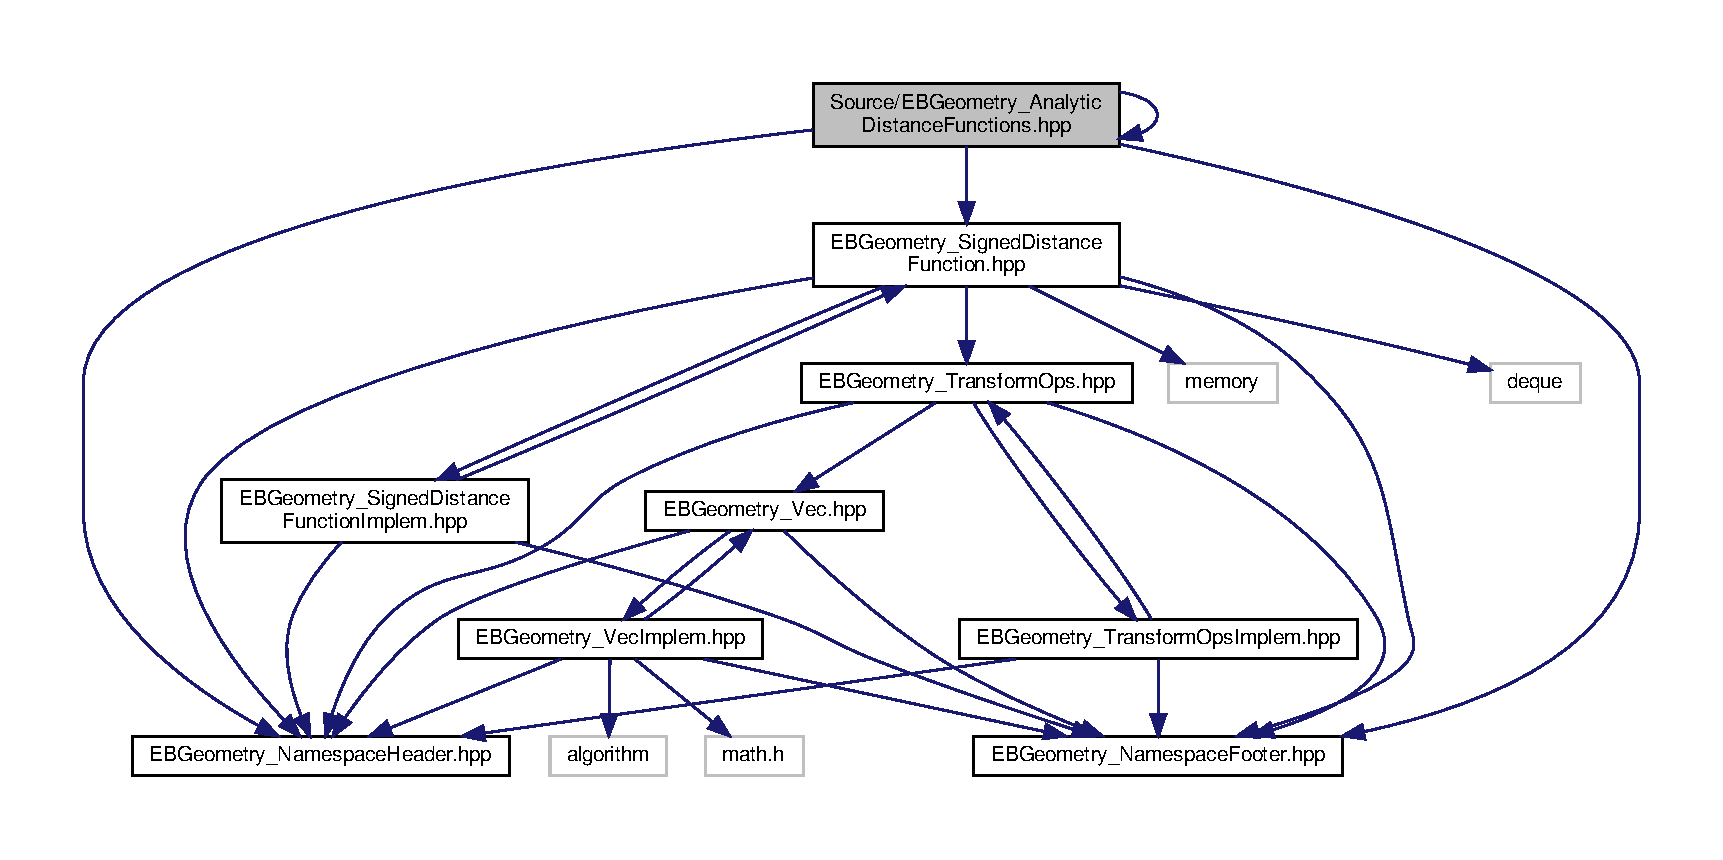
\includegraphics[width=350pt]{EBGeometry__AnalyticDistanceFunctions_8hpp__incl}
\end{center}
\end{figure}
This graph shows which files directly or indirectly include this file\+:
\nopagebreak
\begin{figure}[H]
\begin{center}
\leavevmode
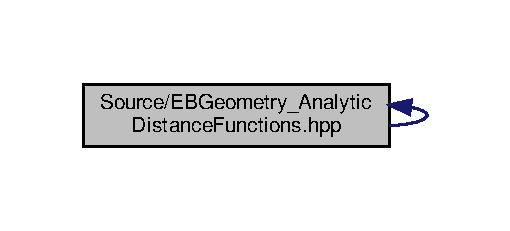
\includegraphics[width=262pt]{EBGeometry__AnalyticDistanceFunctions_8hpp__dep__incl}
\end{center}
\end{figure}
\doxysubsection*{Classes}
\begin{DoxyCompactItemize}
\item 
class \mbox{\hyperlink{classPlaneSDF}{Plane\+SDF$<$ T $>$}}
\begin{DoxyCompactList}\small\item\em Signed distance function for a plane. \end{DoxyCompactList}\item 
class \mbox{\hyperlink{classSphereSDF}{Sphere\+SDF$<$ T $>$}}
\begin{DoxyCompactList}\small\item\em Signed distance field for sphere. \end{DoxyCompactList}\item 
class \mbox{\hyperlink{classBoxSDF}{Box\+SDF$<$ T $>$}}
\begin{DoxyCompactList}\small\item\em Signed distance field for an axis-\/aligned box. \end{DoxyCompactList}\item 
class \mbox{\hyperlink{classTorusSDF}{Torus\+SDF$<$ T $>$}}
\begin{DoxyCompactList}\small\item\em Signed distance field for a torus. \end{DoxyCompactList}\item 
class \mbox{\hyperlink{classCylinderSDF}{Cylinder\+SDF$<$ T $>$}}
\begin{DoxyCompactList}\small\item\em Signed distance field for a cylinder. \end{DoxyCompactList}\item 
class \mbox{\hyperlink{classInfiniteCylinderSDF}{Infinite\+Cylinder\+SDF$<$ T $>$}}
\begin{DoxyCompactList}\small\item\em Inifinitely long cylinder class. Oriented along the y-\/axis. \end{DoxyCompactList}\item 
class \mbox{\hyperlink{classCapsuleSDF}{Capsule\+SDF$<$ T $>$}}
\begin{DoxyCompactList}\small\item\em Capsulate/pill SDF. Basically a cylinder with spherical endcaps, oriented along the specified axis. \end{DoxyCompactList}\item 
class \mbox{\hyperlink{classInfiniteConeSDF}{Infinite\+Cone\+SDF$<$ T $>$}}
\begin{DoxyCompactList}\small\item\em Signed distance field for an infinite cone. Oriented along +z. \end{DoxyCompactList}\item 
class \mbox{\hyperlink{classConeSDF}{Cone\+SDF$<$ T $>$}}
\begin{DoxyCompactList}\small\item\em Signed distance field for an finite cone. Oriented along +z. \end{DoxyCompactList}\end{DoxyCompactItemize}
\doxysubsection*{Functions}
\begin{DoxyCompactItemize}
\item 
{\footnotesize template$<$class T $>$ }\\constexpr const T \& \mbox{\hyperlink{EBGeometry__AnalyticDistanceFunctions_8hpp_afaec2a4dfffd8755efe6a8eca30aae26}{clamp}} (const T \&v, const T \&lo, const T \&hi)
\begin{DoxyCompactList}\small\item\em Clamp function. Returns lo if v $<$ lo and hi if v $>$ hi. Otherwise returns v. \end{DoxyCompactList}\end{DoxyCompactItemize}


\doxysubsection{Detailed Description}
Declaration of various analytic distance functions. 

This file contains various analytic signed distance fields. Some of these also include member function for fetching parameters, and users are free to add such functions also to other shapes. \begin{DoxyAuthor}{Author}
Robert Marskar 
\end{DoxyAuthor}


\doxysubsection{Function Documentation}
\mbox{\Hypertarget{EBGeometry__AnalyticDistanceFunctions_8hpp_afaec2a4dfffd8755efe6a8eca30aae26}\label{EBGeometry__AnalyticDistanceFunctions_8hpp_afaec2a4dfffd8755efe6a8eca30aae26}} 
\index{EBGeometry\_AnalyticDistanceFunctions.hpp@{EBGeometry\_AnalyticDistanceFunctions.hpp}!clamp@{clamp}}
\index{clamp@{clamp}!EBGeometry\_AnalyticDistanceFunctions.hpp@{EBGeometry\_AnalyticDistanceFunctions.hpp}}
\doxysubsubsection{\texorpdfstring{clamp()}{clamp()}}
{\footnotesize\ttfamily template$<$class T $>$ \\
constexpr const T\& clamp (\begin{DoxyParamCaption}\item[{const T \&}]{v,  }\item[{const T \&}]{lo,  }\item[{const T \&}]{hi }\end{DoxyParamCaption})\hspace{0.3cm}{\ttfamily [constexpr]}}



Clamp function. Returns lo if v $<$ lo and hi if v $>$ hi. Otherwise returns v. 


\begin{DoxyParams}[1]{Parameters}
\mbox{\texttt{ in}}  & {\em v} & Value to be clamped. \\
\hline
\mbox{\texttt{ in}}  & {\em lo} & Lower clamping value. \\
\hline
\mbox{\texttt{ in}}  & {\em hi} & Higher clamping value. \\
\hline
\end{DoxyParams}

\hypertarget{EBGeometry__BoundingVolumes_8hpp}{}\section{Source/\+E\+B\+Geometry\+\_\+\+Bounding\+Volumes.hpp File Reference}
\label{EBGeometry__BoundingVolumes_8hpp}\index{Source/\+E\+B\+Geometry\+\_\+\+Bounding\+Volumes.\+hpp@{Source/\+E\+B\+Geometry\+\_\+\+Bounding\+Volumes.\+hpp}}


Declaration of a various bounding volumes used for bounding volume hierarchy.  


{\ttfamily \#include $<$vector$>$}\newline
{\ttfamily \#include \char`\"{}E\+B\+Geometry\+\_\+\+Vec.\+hpp\char`\"{}}\newline
{\ttfamily \#include \char`\"{}E\+B\+Geometry\+\_\+\+Namespace\+Header.\+hpp\char`\"{}}\newline
{\ttfamily \#include \char`\"{}E\+B\+Geometry\+\_\+\+Namespace\+Footer.\+hpp\char`\"{}}\newline
{\ttfamily \#include \char`\"{}E\+B\+Geometry\+\_\+\+Bounding\+Volumes\+Implem.\+hpp\char`\"{}}\newline
Include dependency graph for E\+B\+Geometry\+\_\+\+Bounding\+Volumes.\+hpp\+:\nopagebreak
\begin{figure}[H]
\begin{center}
\leavevmode
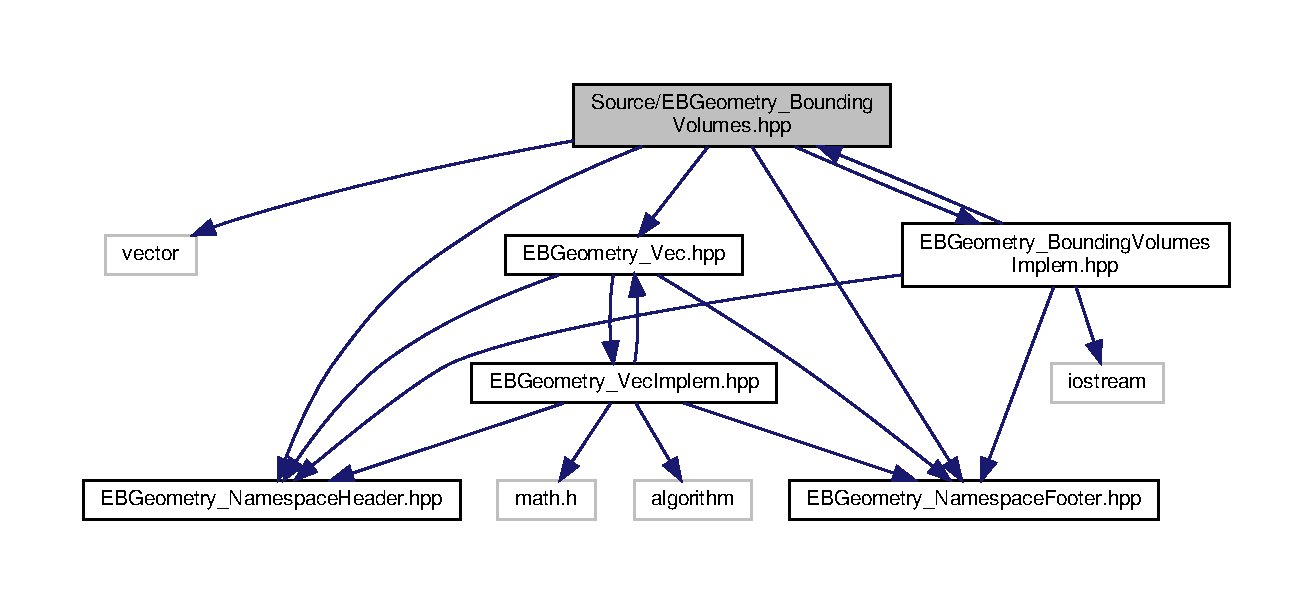
\includegraphics[width=350pt]{EBGeometry__BoundingVolumes_8hpp__incl}
\end{center}
\end{figure}
This graph shows which files directly or indirectly include this file\+:\nopagebreak
\begin{figure}[H]
\begin{center}
\leavevmode
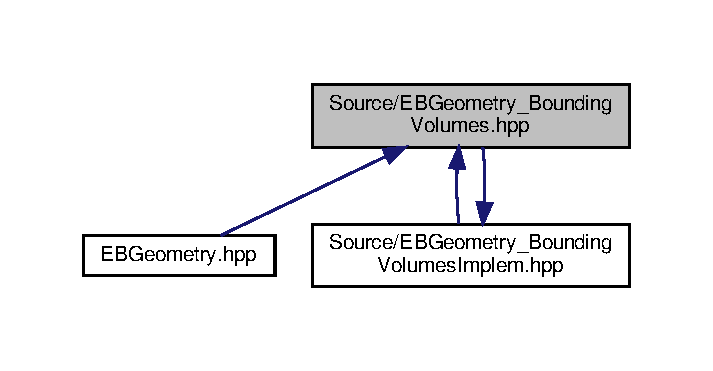
\includegraphics[width=232pt]{EBGeometry__BoundingVolumes_8hpp__dep__incl}
\end{center}
\end{figure}
\subsection*{Classes}
\begin{DoxyCompactItemize}
\item 
class \hyperlink{classBoundingVolumes_1_1BoundingSphereT}{Bounding\+Volumes\+::\+Bounding\+Sphere\+T$<$ T $>$}
\begin{DoxyCompactList}\small\item\em Class which encloses a set of points using a bounding sphere. \end{DoxyCompactList}\item 
class \hyperlink{classBoundingVolumes_1_1AABBT}{Bounding\+Volumes\+::\+A\+A\+B\+B\+T$<$ T $>$}
\begin{DoxyCompactList}\small\item\em Axis-\/aligned bounding box as bounding volume. \end{DoxyCompactList}\end{DoxyCompactItemize}
\subsection*{Namespaces}
\begin{DoxyCompactItemize}
\item 
 \hyperlink{namespaceBoundingVolumes}{Bounding\+Volumes}
\begin{DoxyCompactList}\small\item\em Namespace for encapsulating various bounding volumes for usage with B\+V\+Hs. \end{DoxyCompactList}\end{DoxyCompactItemize}
\subsection*{Functions}
\begin{DoxyCompactItemize}
\item 
{\footnotesize template$<$class T $>$ }\\bool \hyperlink{namespaceBoundingVolumes_af35f33c5f319a466550d9ad1040beced}{Bounding\+Volumes\+::intersects} (const Bounding\+SphereT$<$ T $>$ \&a\+\_\+u, const Bounding\+SphereT$<$ T $>$ \&a\+\_\+v) noexcept
\begin{DoxyCompactList}\small\item\em Intersection method for testing if two bounding spheres overlap. \end{DoxyCompactList}\item 
{\footnotesize template$<$class T $>$ }\\bool \hyperlink{namespaceBoundingVolumes_a5c360ccd42017c01acbe1caf2cfd1efe}{Bounding\+Volumes\+::intersects} (const A\+A\+B\+BT$<$ T $>$ \&a\+\_\+u, const A\+A\+B\+BT$<$ T $>$ \&a\+\_\+v) noexcept
\begin{DoxyCompactList}\small\item\em Intersection method for testing if two bounding boxes overlap. \end{DoxyCompactList}\item 
{\footnotesize template$<$class T $>$ }\\T \hyperlink{namespaceBoundingVolumes_a4f159289c317e02beedb4b38136ad692}{Bounding\+Volumes\+::get\+Overlapping\+Volume} (const Bounding\+SphereT$<$ T $>$ \&a\+\_\+u, const Bounding\+SphereT$<$ T $>$ \&a\+\_\+v) noexcept
\begin{DoxyCompactList}\small\item\em Compute the overlapping volume between two bounding spheres. \end{DoxyCompactList}\item 
{\footnotesize template$<$class T $>$ }\\T \hyperlink{namespaceBoundingVolumes_ae5716e39e88aaeec0c204f453cac2acd}{Bounding\+Volumes\+::get\+Overlapping\+Volume} (const A\+A\+B\+BT$<$ T $>$ \&a\+\_\+u, const A\+A\+B\+BT$<$ T $>$ \&a\+\_\+v) noexcept
\begin{DoxyCompactList}\small\item\em Compute the overlapping volume between two bounding boxes. \end{DoxyCompactList}\end{DoxyCompactItemize}


\subsection{Detailed Description}
Declaration of a various bounding volumes used for bounding volume hierarchy. 

\begin{DoxyAuthor}{Author}
Robert Marskar 
\end{DoxyAuthor}

\hypertarget{EBGeometry__BoundingVolumesImplem_8hpp}{}\doxysection{/home/runner/work/\+E\+B\+Geometry/\+E\+B\+Geometry/\+Source/\+E\+B\+Geometry\+\_\+\+Bounding\+Volumes\+Implem.hpp File Reference}
\label{EBGeometry__BoundingVolumesImplem_8hpp}\index{/home/runner/work/EBGeometry/EBGeometry/Source/EBGeometry\_BoundingVolumesImplem.hpp@{/home/runner/work/EBGeometry/EBGeometry/Source/EBGeometry\_BoundingVolumesImplem.hpp}}


Implementation of \mbox{\hyperlink{EBGeometry__BoundingVolumes_8hpp}{E\+B\+Geometry\+\_\+\+Bounding\+Volumes.\+hpp}}.  


{\ttfamily \#include $<$iostream$>$}\newline
{\ttfamily \#include \char`\"{}E\+B\+Geometry\+\_\+\+Bounding\+Volumes.\+hpp\char`\"{}}\newline
{\ttfamily \#include \char`\"{}E\+B\+Geometry\+\_\+\+Namespace\+Header.\+hpp\char`\"{}}\newline
{\ttfamily \#include \char`\"{}E\+B\+Geometry\+\_\+\+Namespace\+Footer.\+hpp\char`\"{}}\newline
Include dependency graph for E\+B\+Geometry\+\_\+\+Bounding\+Volumes\+Implem.\+hpp\+:
\nopagebreak
\begin{figure}[H]
\begin{center}
\leavevmode
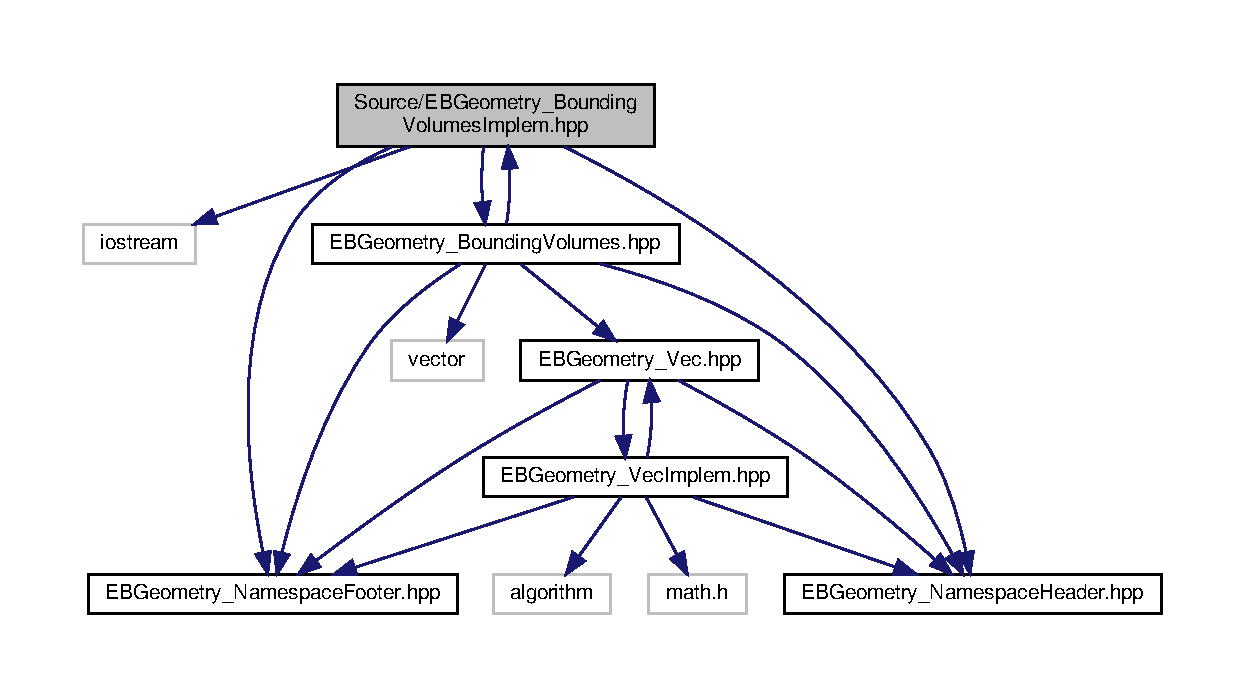
\includegraphics[width=350pt]{EBGeometry__BoundingVolumesImplem_8hpp__incl}
\end{center}
\end{figure}
This graph shows which files directly or indirectly include this file\+:
\nopagebreak
\begin{figure}[H]
\begin{center}
\leavevmode
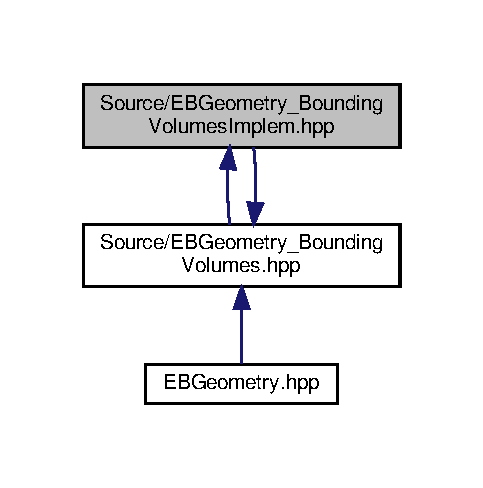
\includegraphics[width=262pt]{EBGeometry__BoundingVolumesImplem_8hpp__dep__incl}
\end{center}
\end{figure}
\doxysubsection*{Namespaces}
\begin{DoxyCompactItemize}
\item 
 \mbox{\hyperlink{namespaceBoundingVolumes}{Bounding\+Volumes}}
\begin{DoxyCompactList}\small\item\em Namespace for encapsulating various bounding volumes for usage with B\+V\+Hs. \end{DoxyCompactList}\end{DoxyCompactItemize}
\doxysubsection*{Functions}
\begin{DoxyCompactItemize}
\item 
{\footnotesize template$<$class T $>$ }\\bool \mbox{\hyperlink{namespaceBoundingVolumes_af35f33c5f319a466550d9ad1040beced}{Bounding\+Volumes\+::intersects}} (const Bounding\+SphereT$<$ T $>$ \&a\+\_\+u, const Bounding\+SphereT$<$ T $>$ \&a\+\_\+v) noexcept
\begin{DoxyCompactList}\small\item\em Intersection method for testing if two bounding spheres overlap. \end{DoxyCompactList}\item 
{\footnotesize template$<$class T $>$ }\\bool \mbox{\hyperlink{namespaceBoundingVolumes_a5c360ccd42017c01acbe1caf2cfd1efe}{Bounding\+Volumes\+::intersects}} (const A\+A\+B\+BT$<$ T $>$ \&a\+\_\+u, const A\+A\+B\+BT$<$ T $>$ \&a\+\_\+v) noexcept
\begin{DoxyCompactList}\small\item\em Intersection method for testing if two bounding boxes overlap. \end{DoxyCompactList}\item 
{\footnotesize template$<$class T $>$ }\\T \mbox{\hyperlink{namespaceBoundingVolumes_a4f159289c317e02beedb4b38136ad692}{Bounding\+Volumes\+::get\+Overlapping\+Volume}} (const Bounding\+SphereT$<$ T $>$ \&a\+\_\+u, const Bounding\+SphereT$<$ T $>$ \&a\+\_\+v) noexcept
\begin{DoxyCompactList}\small\item\em Compute the overlapping volume between two bounding spheres. \end{DoxyCompactList}\item 
{\footnotesize template$<$class T $>$ }\\T \mbox{\hyperlink{namespaceBoundingVolumes_ae5716e39e88aaeec0c204f453cac2acd}{Bounding\+Volumes\+::get\+Overlapping\+Volume}} (const A\+A\+B\+BT$<$ T $>$ \&a\+\_\+u, const A\+A\+B\+BT$<$ T $>$ \&a\+\_\+v) noexcept
\begin{DoxyCompactList}\small\item\em Compute the overlapping volume between two bounding boxes. \end{DoxyCompactList}\end{DoxyCompactItemize}


\doxysubsection{Detailed Description}
Implementation of \mbox{\hyperlink{EBGeometry__BoundingVolumes_8hpp}{E\+B\+Geometry\+\_\+\+Bounding\+Volumes.\+hpp}}. 

\begin{DoxyAuthor}{Author}
Robert Marskar 
\end{DoxyAuthor}

\hypertarget{EBGeometry__BVH_8hpp}{}\section{Source/\+E\+B\+Geometry\+\_\+\+B\+VH.hpp File Reference}
\label{EBGeometry__BVH_8hpp}\index{Source/\+E\+B\+Geometry\+\_\+\+B\+V\+H.\+hpp@{Source/\+E\+B\+Geometry\+\_\+\+B\+V\+H.\+hpp}}


Declaration of a bounding volume hierarchy (\hyperlink{namespaceBVH}{B\+VH}) class.  


{\ttfamily \#include $<$memory$>$}\newline
{\ttfamily \#include $<$vector$>$}\newline
{\ttfamily \#include $<$functional$>$}\newline
{\ttfamily \#include $<$queue$>$}\newline
{\ttfamily \#include \char`\"{}E\+B\+Geometry\+\_\+\+Vec.\+hpp\char`\"{}}\newline
{\ttfamily \#include \char`\"{}E\+B\+Geometry\+\_\+\+Namespace\+Header.\+hpp\char`\"{}}\newline
{\ttfamily \#include \char`\"{}E\+B\+Geometry\+\_\+\+Namespace\+Footer.\+hpp\char`\"{}}\newline
{\ttfamily \#include \char`\"{}E\+B\+Geometry\+\_\+\+B\+V\+H\+Implem.\+hpp\char`\"{}}\newline
Include dependency graph for E\+B\+Geometry\+\_\+\+B\+V\+H.\+hpp\+:\nopagebreak
\begin{figure}[H]
\begin{center}
\leavevmode
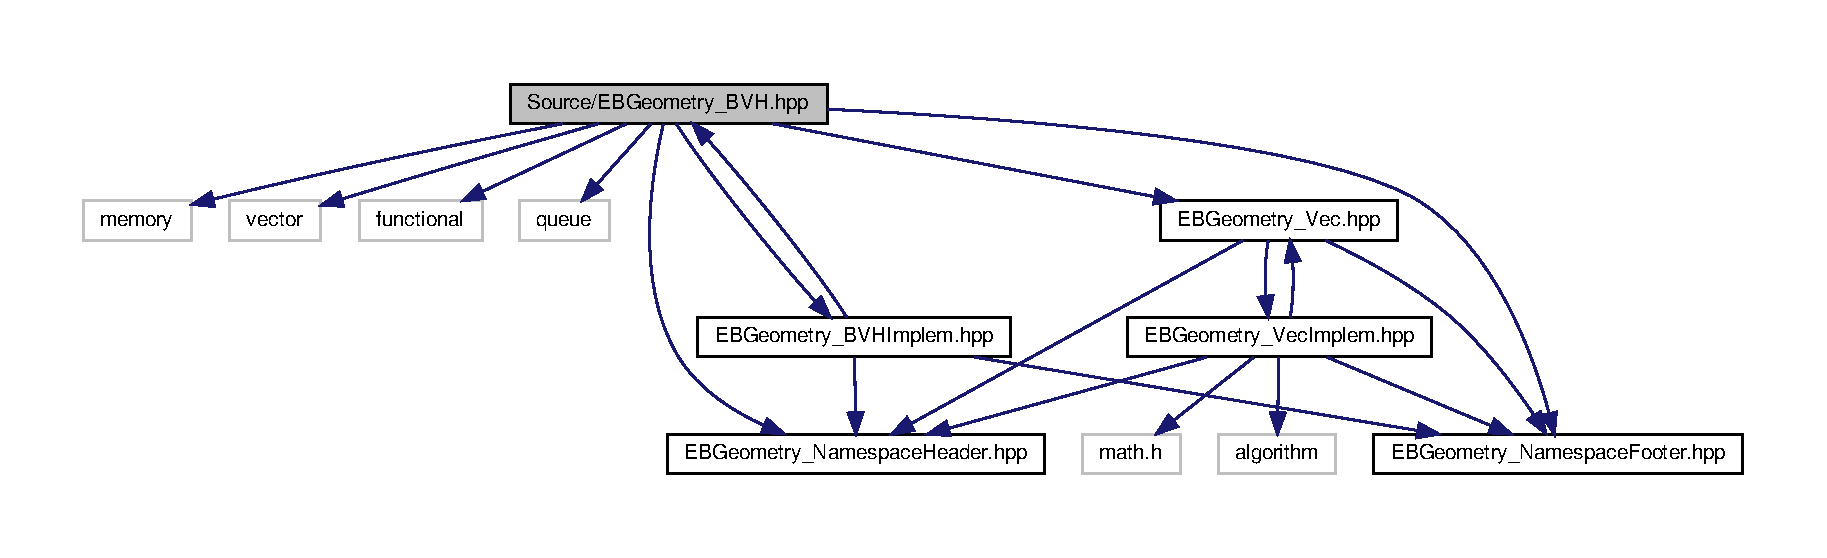
\includegraphics[width=350pt]{EBGeometry__BVH_8hpp__incl}
\end{center}
\end{figure}
This graph shows which files directly or indirectly include this file\+:\nopagebreak
\begin{figure}[H]
\begin{center}
\leavevmode
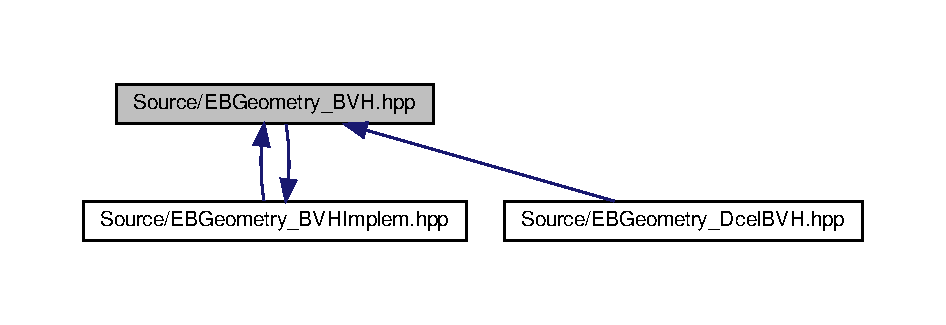
\includegraphics[width=350pt]{EBGeometry__BVH_8hpp__dep__incl}
\end{center}
\end{figure}
\subsection*{Classes}
\begin{DoxyCompactItemize}
\item 
class \hyperlink{classBVH_1_1NodeT}{B\+V\+H\+::\+Node\+T$<$ T, P, B\+V, K $>$}
\begin{DoxyCompactList}\small\item\em Forward declare the \hyperlink{namespaceBVH}{B\+VH} node since it is needed for the polymorphic lambdas. \end{DoxyCompactList}\item 
class \hyperlink{classBVH_1_1LinearNodeT}{B\+V\+H\+::\+Linear\+Node\+T$<$ T, P, B\+V, K $>$}
\begin{DoxyCompactList}\small\item\em Forward declare linear node class. \end{DoxyCompactList}\item 
class \hyperlink{classBVH_1_1LinearBVH}{B\+V\+H\+::\+Linear\+B\+V\+H$<$ T, P, B\+V, K $>$}
\begin{DoxyCompactList}\small\item\em Forward declare linear \hyperlink{namespaceBVH}{B\+VH} class. \end{DoxyCompactList}\item 
class \hyperlink{classBVH_1_1NodeT}{B\+V\+H\+::\+Node\+T$<$ T, P, B\+V, K $>$}
\begin{DoxyCompactList}\small\item\em Forward declare the \hyperlink{namespaceBVH}{B\+VH} node since it is needed for the polymorphic lambdas. \end{DoxyCompactList}\item 
class \hyperlink{classBVH_1_1LinearNodeT}{B\+V\+H\+::\+Linear\+Node\+T$<$ T, P, B\+V, K $>$}
\begin{DoxyCompactList}\small\item\em Forward declare linear node class. \end{DoxyCompactList}\item 
class \hyperlink{classBVH_1_1LinearBVH}{B\+V\+H\+::\+Linear\+B\+V\+H$<$ T, P, B\+V, K $>$}
\begin{DoxyCompactList}\small\item\em Forward declare linear \hyperlink{namespaceBVH}{B\+VH} class. \end{DoxyCompactList}\end{DoxyCompactItemize}
\subsection*{Namespaces}
\begin{DoxyCompactItemize}
\item 
 \hyperlink{namespaceBVH}{B\+VH}
\begin{DoxyCompactList}\small\item\em Namespace for various bounding volume heirarchy (\hyperlink{namespaceBVH}{B\+VH}) functionality. \end{DoxyCompactList}\end{DoxyCompactItemize}
\subsection*{Typedefs}
\begin{DoxyCompactItemize}
\item 
{\footnotesize template$<$class P $>$ }\\using \hyperlink{namespaceBVH_aa1e753bda451b85cd5b948722a2ad7c7}{B\+V\+H\+::\+Primitive\+ListT} = std\+::vector$<$ std\+::shared\+\_\+ptr$<$ const P $>$ $>$
\begin{DoxyCompactList}\small\item\em Alias to cut down on typing. \end{DoxyCompactList}\item 
{\footnotesize template$<$class T , class P , class BV , int K$>$ }\\using \hyperlink{namespaceBVH_afef1c5979c34a11d23b756cc09654bf9}{B\+V\+H\+::\+Stop\+FunctionT} = std\+::function$<$ bool(const NodeT$<$ T, P, BV, K $>$ \&a\+\_\+node)$>$
\begin{DoxyCompactList}\small\item\em Stop function for deciding when a \hyperlink{namespaceBVH}{B\+VH} node can\textquotesingle{}t be divided into sub-\/volumes. \end{DoxyCompactList}\item 
{\footnotesize template$<$class P , int K$>$ }\\using \hyperlink{namespaceBVH_a7c33d54da9893d506709b2ca96b76f55}{B\+V\+H\+::\+PartitionerT} = std\+::function$<$ std\+::array$<$ Primitive\+ListT$<$ P $>$, K $>$(const Primitive\+ListT$<$ P $>$ \&a\+\_\+primitives)$>$
\begin{DoxyCompactList}\small\item\em Polymorphic partitioner for splitting a list of primitives into K new lists of primitives. \end{DoxyCompactList}\item 
{\footnotesize template$<$class P , class BV $>$ }\\using \hyperlink{namespaceBVH_a245702d7eff40cdaedb5dff68c25a88a}{B\+V\+H\+::\+B\+V\+ConstructorT} = std\+::function$<$ BV(const std\+::shared\+\_\+ptr$<$ const P $>$ \&a\+\_\+primitive)$>$
\begin{DoxyCompactList}\small\item\em Constructor method for creating bounding volumes from a list of primitives. \end{DoxyCompactList}\end{DoxyCompactItemize}
\subsection*{Enumerations}
\begin{DoxyCompactItemize}
\item 
enum \hyperlink{namespaceBVH_a3ddb7b34ac1deb3baed2f32d9eacbe5b}{B\+V\+H\+::\+Prune} \{ {\bfseries Stack}, 
{\bfseries Ordered}, 
{\bfseries Unordered}
 \}\begin{DoxyCompactList}\small\item\em Typename for identifying algorithms various algorithms during tree traversel. \end{DoxyCompactList}
\end{DoxyCompactItemize}


\subsection{Detailed Description}
Declaration of a bounding volume hierarchy (\hyperlink{namespaceBVH}{B\+VH}) class. 

\begin{DoxyAuthor}{Author}
Robert Marskar 
\end{DoxyAuthor}

\hypertarget{EBGeometry__BVHImplem_8hpp}{}\doxysection{Source/\+E\+B\+Geometry\+\_\+\+B\+V\+H\+Implem.hpp File Reference}
\label{EBGeometry__BVHImplem_8hpp}\index{Source/EBGeometry\_BVHImplem.hpp@{Source/EBGeometry\_BVHImplem.hpp}}


Implementation of \mbox{\hyperlink{EBGeometry__BVH_8hpp}{E\+B\+Geometry\+\_\+\+B\+V\+H.\+hpp}}.  


{\ttfamily \#include $<$stack$>$}\newline
{\ttfamily \#include \char`\"{}E\+B\+Geometry\+\_\+\+B\+V\+H.\+hpp\char`\"{}}\newline
{\ttfamily \#include \char`\"{}E\+B\+Geometry\+\_\+\+Namespace\+Header.\+hpp\char`\"{}}\newline
{\ttfamily \#include \char`\"{}E\+B\+Geometry\+\_\+\+Namespace\+Footer.\+hpp\char`\"{}}\newline
Include dependency graph for E\+B\+Geometry\+\_\+\+B\+V\+H\+Implem.\+hpp\+:
\nopagebreak
\begin{figure}[H]
\begin{center}
\leavevmode
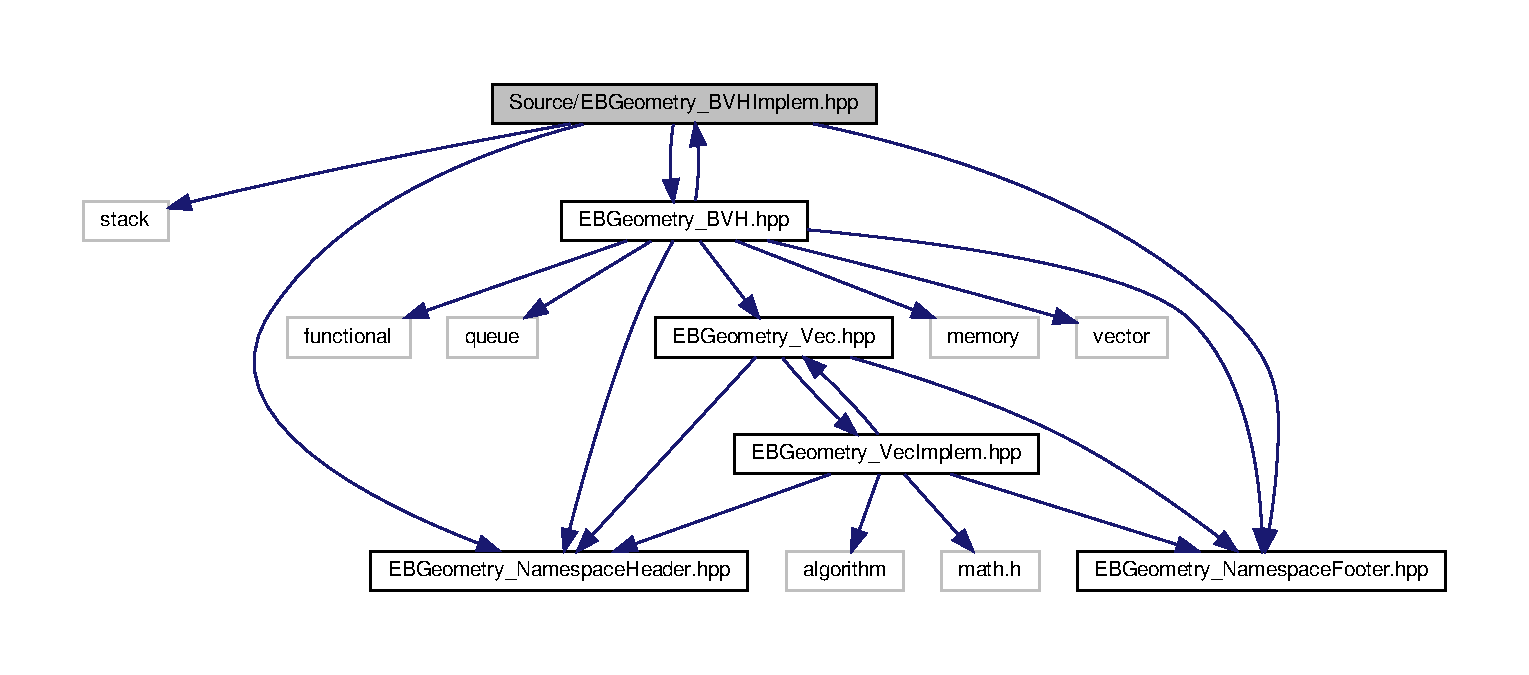
\includegraphics[width=350pt]{EBGeometry__BVHImplem_8hpp__incl}
\end{center}
\end{figure}
This graph shows which files directly or indirectly include this file\+:
\nopagebreak
\begin{figure}[H]
\begin{center}
\leavevmode
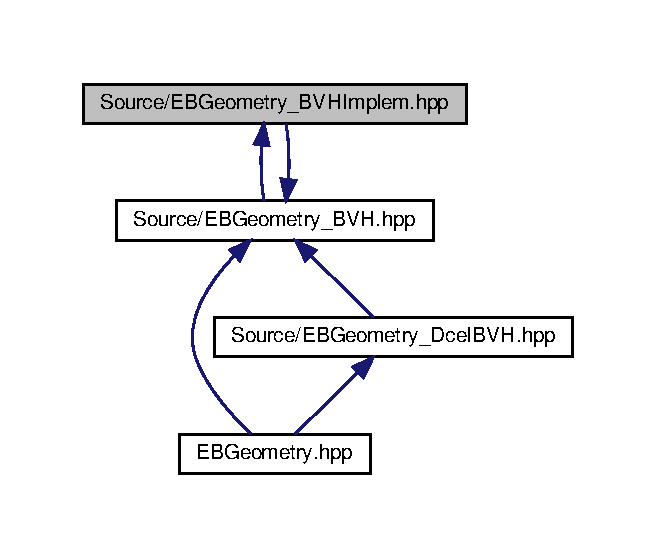
\includegraphics[width=303pt]{EBGeometry__BVHImplem_8hpp__dep__incl}
\end{center}
\end{figure}
\doxysubsection*{Namespaces}
\begin{DoxyCompactItemize}
\item 
 \mbox{\hyperlink{namespaceBVH}{B\+VH}}
\begin{DoxyCompactList}\small\item\em Namespace for various bounding volume hierarchy (\mbox{\hyperlink{namespaceBVH}{B\+VH}}) functionality. \end{DoxyCompactList}\end{DoxyCompactItemize}


\doxysubsection{Detailed Description}
Implementation of \mbox{\hyperlink{EBGeometry__BVH_8hpp}{E\+B\+Geometry\+\_\+\+B\+V\+H.\+hpp}}. 

\begin{DoxyAuthor}{Author}
Robert Marskar 
\end{DoxyAuthor}

\hypertarget{EBGeometry__Dcel_8hpp}{}\section{Source/\+E\+B\+Geometry\+\_\+\+Dcel.hpp File Reference}
\label{EBGeometry__Dcel_8hpp}\index{Source/\+E\+B\+Geometry\+\_\+\+Dcel.\+hpp@{Source/\+E\+B\+Geometry\+\_\+\+Dcel.\+hpp}}


Namespace documentation.  


{\ttfamily \#include \char`\"{}E\+B\+Geometry\+\_\+\+Namespace\+Header.\+hpp\char`\"{}}\newline
{\ttfamily \#include \char`\"{}E\+B\+Geometry\+\_\+\+Namespace\+Footer.\+hpp\char`\"{}}\newline
Include dependency graph for E\+B\+Geometry\+\_\+\+Dcel.\+hpp\+:\nopagebreak
\begin{figure}[H]
\begin{center}
\leavevmode
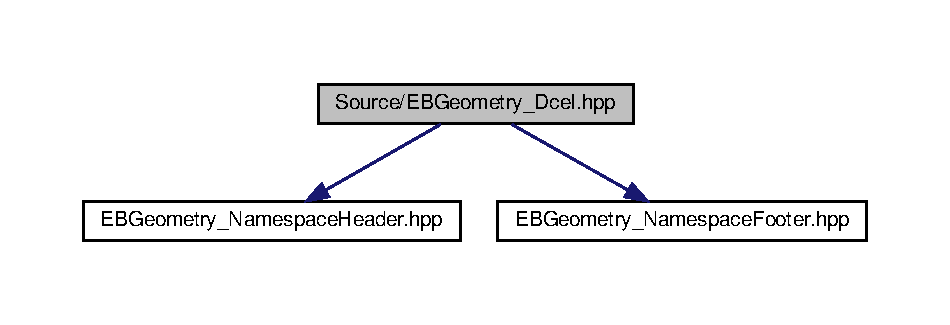
\includegraphics[width=350pt]{EBGeometry__Dcel_8hpp__incl}
\end{center}
\end{figure}
This graph shows which files directly or indirectly include this file\+:\nopagebreak
\begin{figure}[H]
\begin{center}
\leavevmode
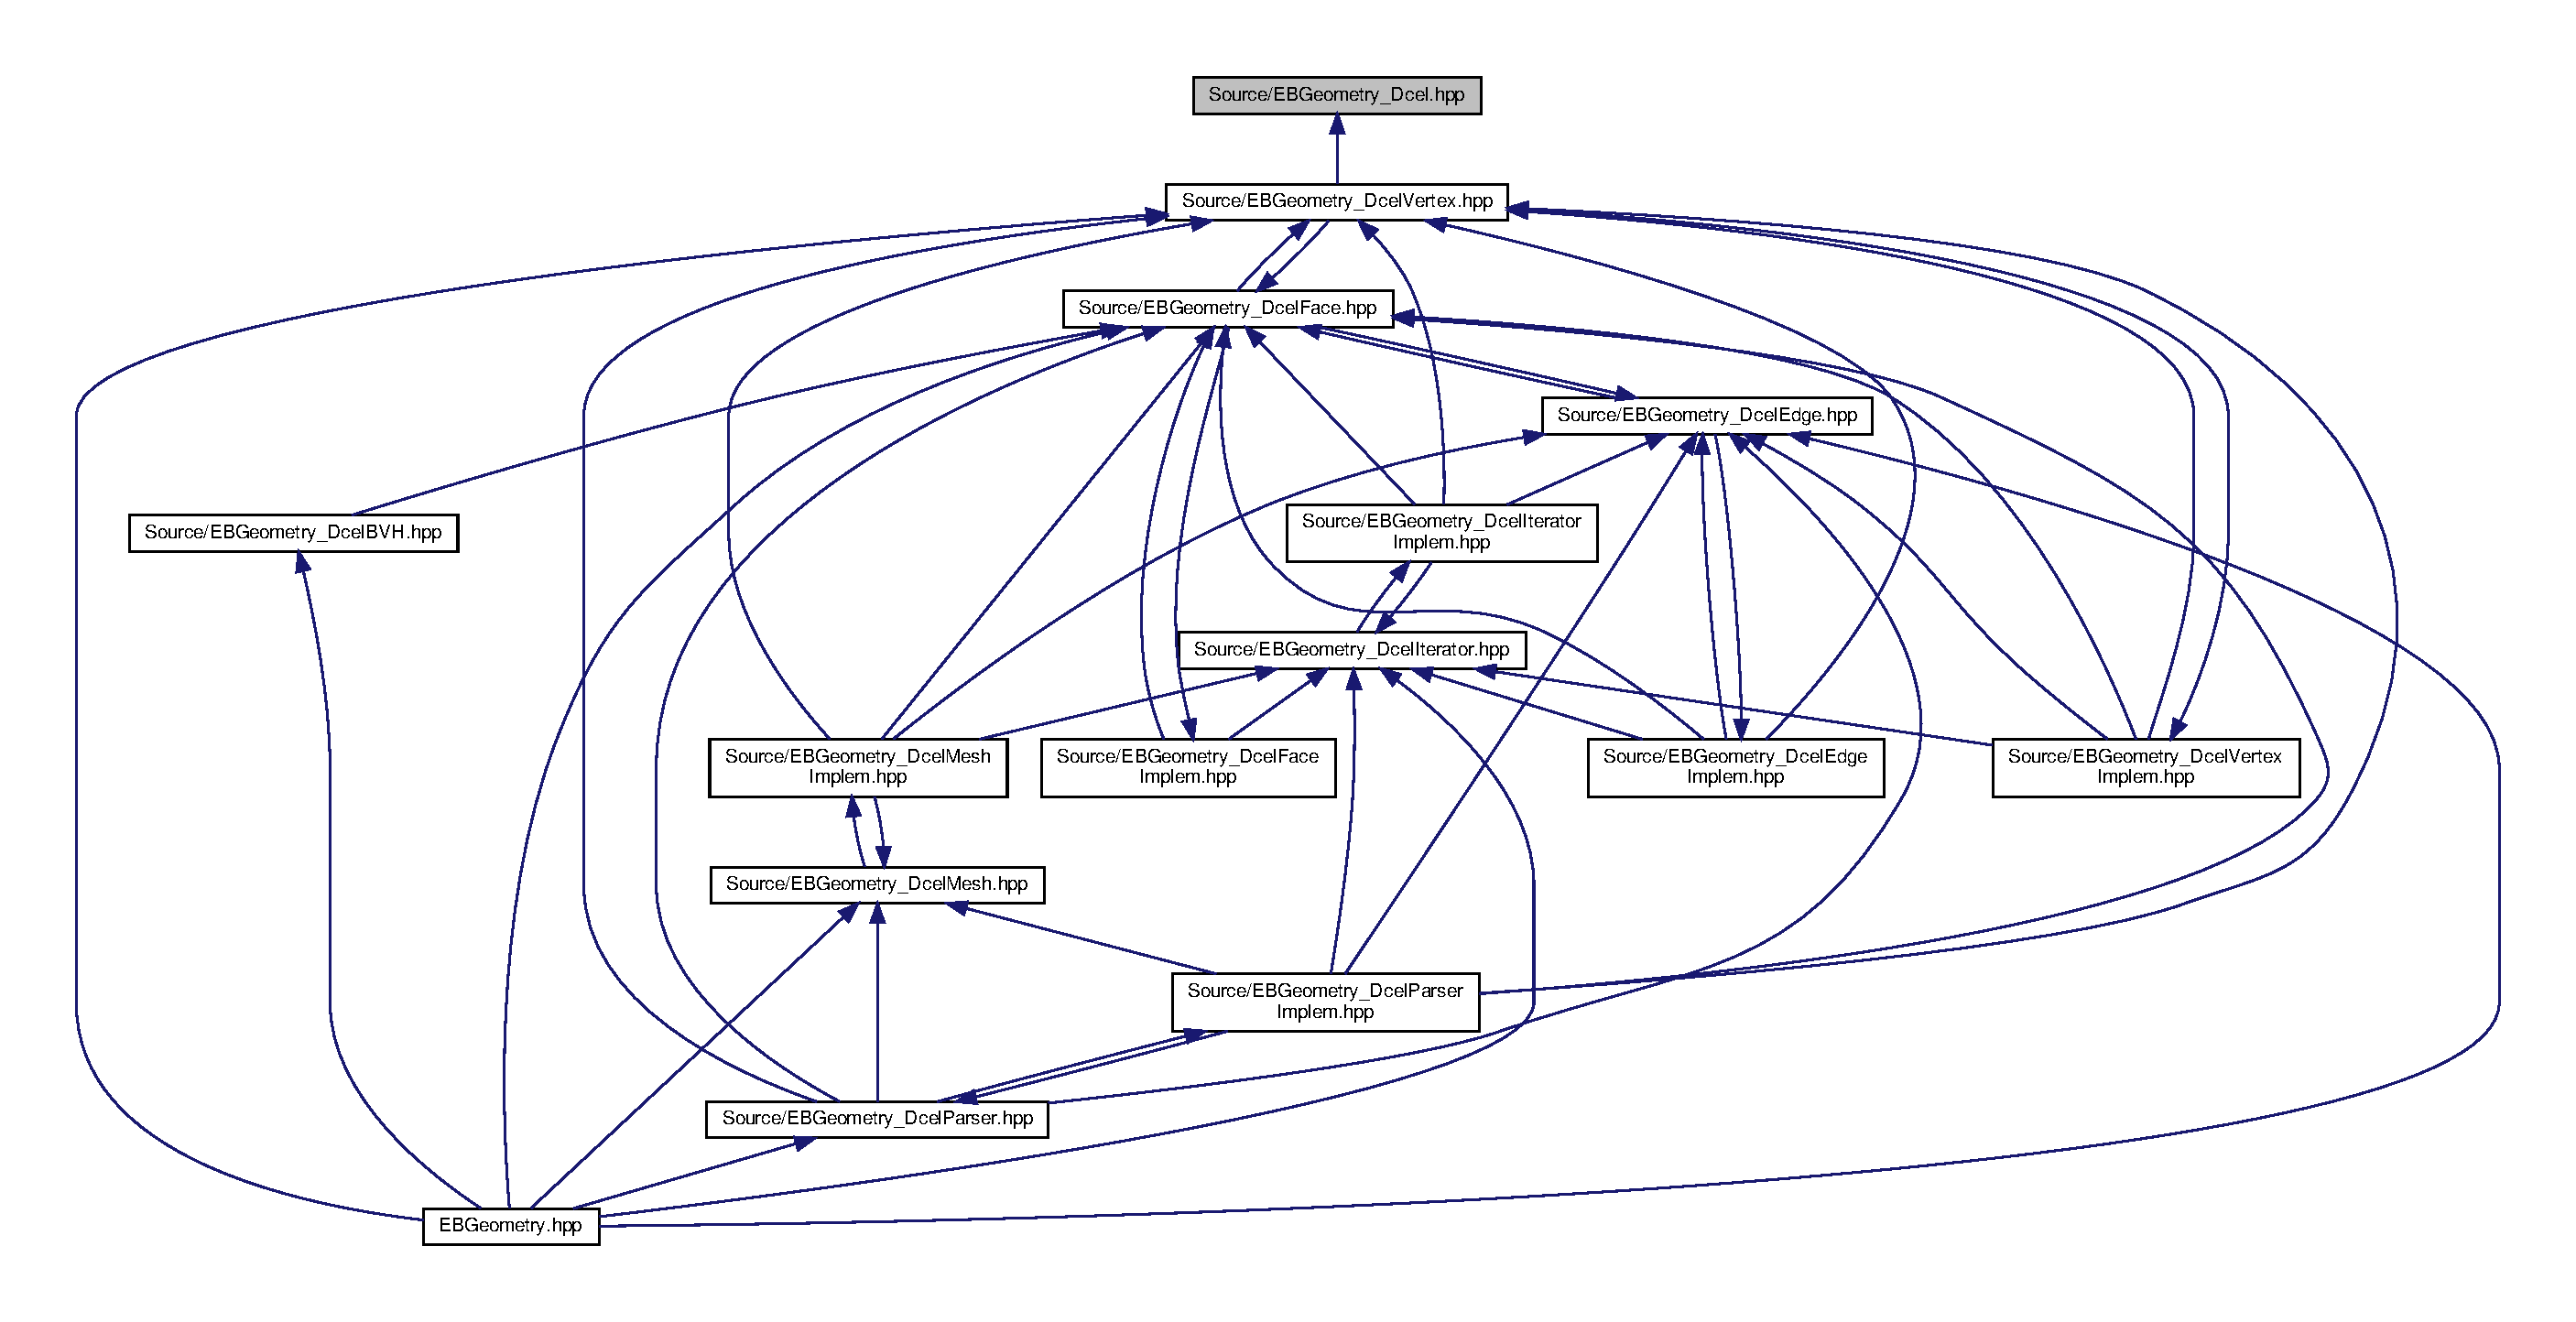
\includegraphics[width=350pt]{EBGeometry__Dcel_8hpp__dep__incl}
\end{center}
\end{figure}
\subsection*{Namespaces}
\begin{DoxyCompactItemize}
\item 
 \hyperlink{namespaceDcel}{Dcel}
\begin{DoxyCompactList}\small\item\em Namespace containing various double-\/connected edge list (D\+C\+EL) functionality. \end{DoxyCompactList}\end{DoxyCompactItemize}


\subsection{Detailed Description}
Namespace documentation. 

\begin{DoxyAuthor}{Author}
Robert Marskar 
\end{DoxyAuthor}

\hypertarget{EBGeometry__DcelBVH_8hpp}{}\section{Source/\+E\+B\+Geometry\+\_\+\+Dcel\+B\+VH.hpp File Reference}
\label{EBGeometry__DcelBVH_8hpp}\index{Source/\+E\+B\+Geometry\+\_\+\+Dcel\+B\+V\+H.\+hpp@{Source/\+E\+B\+Geometry\+\_\+\+Dcel\+B\+V\+H.\+hpp}}


File which contains partitioners and lambdas for enclosing dcel\+\_\+face in bounding volume heirarchies.  


{\ttfamily \#include \char`\"{}E\+B\+Geometry\+\_\+\+B\+V\+H.\+hpp\char`\"{}}\newline
{\ttfamily \#include \char`\"{}E\+B\+Geometry\+\_\+\+Dcel\+Face.\+hpp\char`\"{}}\newline
{\ttfamily \#include \char`\"{}E\+B\+Geometry\+\_\+\+Namespace\+Header.\+hpp\char`\"{}}\newline
{\ttfamily \#include \char`\"{}E\+B\+Geometry\+\_\+\+Namespace\+Footer.\+hpp\char`\"{}}\newline
Include dependency graph for E\+B\+Geometry\+\_\+\+Dcel\+B\+V\+H.\+hpp\+:\nopagebreak
\begin{figure}[H]
\begin{center}
\leavevmode
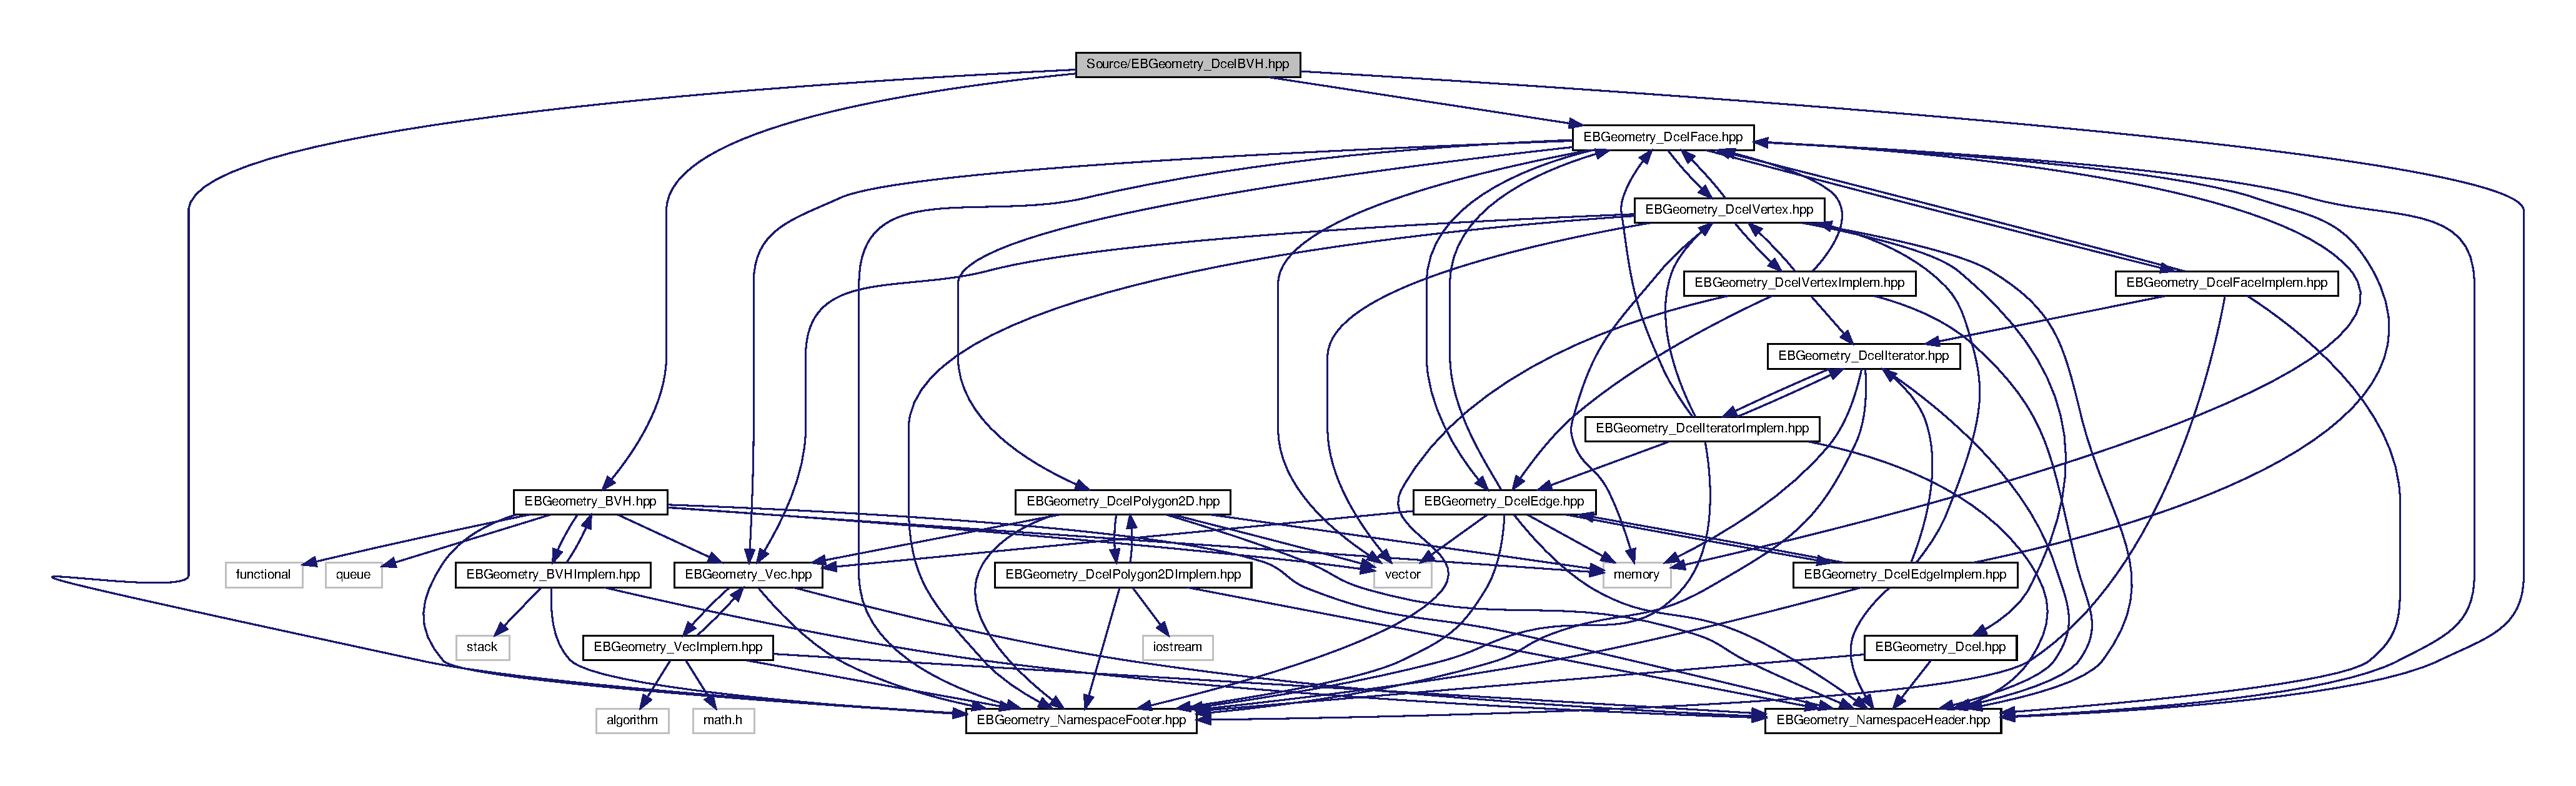
\includegraphics[width=350pt]{EBGeometry__DcelBVH_8hpp__incl}
\end{center}
\end{figure}
This graph shows which files directly or indirectly include this file\+:\nopagebreak
\begin{figure}[H]
\begin{center}
\leavevmode
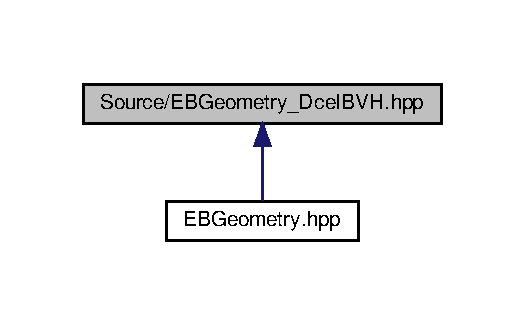
\includegraphics[width=252pt]{EBGeometry__DcelBVH_8hpp__dep__incl}
\end{center}
\end{figure}
\subsection*{Namespaces}
\begin{DoxyCompactItemize}
\item 
 \hyperlink{namespaceDcel}{Dcel}
\begin{DoxyCompactList}\small\item\em Namespace containing various double-\/connected edge list (D\+C\+EL) functionality. \end{DoxyCompactList}\end{DoxyCompactItemize}
\subsection*{Typedefs}
\begin{DoxyCompactItemize}
\item 
\mbox{\Hypertarget{namespaceDcel_a69f60bf0111d66715bf4f7a8e22645e6}\label{namespaceDcel_a69f60bf0111d66715bf4f7a8e22645e6}} 
{\footnotesize template$<$class T $>$ }\\using \hyperlink{namespaceDcel_a69f60bf0111d66715bf4f7a8e22645e6}{Dcel\+::\+Primitive\+List} = std\+::vector$<$ std\+::shared\+\_\+ptr$<$ const \hyperlink{classDcel_1_1FaceT}{Dcel\+::\+FaceT}$<$ T $>$ $>$ $>$
\begin{DoxyCompactList}\small\item\em Alias for which primitives are used in the \hyperlink{namespaceBVH}{B\+VH}. For D\+C\+EL meshes the primitive is a polygon face. \end{DoxyCompactList}\end{DoxyCompactItemize}
\subsection*{Variables}
\begin{DoxyCompactItemize}
\item 
\mbox{\Hypertarget{namespaceDcel_a4db11eb50441e7c4e6c3ae796a202024}\label{namespaceDcel_a4db11eb50441e7c4e6c3ae796a202024}} 
constexpr int \hyperlink{namespaceDcel_a4db11eb50441e7c4e6c3ae796a202024}{Dcel\+::primitives\+Per\+Leaf\+Node} = 1
\begin{DoxyCompactList}\small\item\em This is the lowest number of a primitives that a \hyperlink{namespaceBVH}{B\+VH} node is allowed to enclose. \end{DoxyCompactList}\item 
{\footnotesize template$<$class T , class BV $>$ }\\\hyperlink{namespaceBVH_a245702d7eff40cdaedb5dff68c25a88a}{B\+V\+H\+::\+B\+V\+ConstructorT}$<$ FaceT$<$ T $>$, BV $>$ \hyperlink{namespaceDcel_a628449c42ce3f2784ca018f2a3c88a11}{Dcel\+::default\+B\+V\+Constructor}
\begin{DoxyCompactList}\small\item\em Bounding volume constructor for a D\+C\+EL face. \end{DoxyCompactList}\item 
{\footnotesize template$<$class T , class BV , int K$>$ }\\\hyperlink{namespaceBVH_afef1c5979c34a11d23b756cc09654bf9}{B\+V\+H\+::\+Stop\+FunctionT}$<$ T, FaceT$<$ T $>$, BV, K $>$ \hyperlink{namespaceDcel_a45e9f2554a8d9ea01164cd51f787f989}{Dcel\+::default\+Stop\+Function}
\begin{DoxyCompactList}\small\item\em Default stop function. This function terminates the division process if a \hyperlink{namespaceBVH}{B\+VH} node has only one primitive. \end{DoxyCompactList}\item 
{\footnotesize template$<$class T , int K$>$ }\\\hyperlink{namespaceBVH_a7c33d54da9893d506709b2ca96b76f55}{B\+V\+H\+::\+PartitionerT}$<$ FaceT$<$ T $>$, K $>$ \hyperlink{namespaceDcel_ab4f869248e23d47bb01ad06c76288fef}{Dcel\+::spatial\+Split\+Partitioner}
\begin{DoxyCompactList}\small\item\em Default partitioner function for subdividing into K sub-\/volumes. \end{DoxyCompactList}\item 
{\footnotesize template$<$class T , int K$>$ }\\\hyperlink{namespaceBVH_a7c33d54da9893d506709b2ca96b76f55}{B\+V\+H\+::\+PartitionerT}$<$ FaceT$<$ T $>$, K $>$ \hyperlink{namespaceDcel_a08217ffcd4cfc6f58a3b0b3f780fc611}{Dcel\+::spatial\+Split\+Binary\+Partitioner}
\begin{DoxyCompactList}\small\item\em Binary partitioner based on spatial splits. \end{DoxyCompactList}\end{DoxyCompactItemize}


\subsection{Detailed Description}
File which contains partitioners and lambdas for enclosing dcel\+\_\+face in bounding volume heirarchies. 

This file contains various useful \char`\"{}default\char`\"{} routines for determining how a D\+C\+EL mesh should be partitioned in a bounding volume hierarchy. This includes the required functions for 1) Constructing bounding volumes (default\+B\+V\+Constructor). 2) Stopping the sub-\/division process (default\+Stop\+Function) 3) Partitioning one bounding volume into subvolumes. These are the functions a) default\+Partition\+Function(...). This partitions the primitives into two half-\/spaces based on where the primitive centroids are located. b) partition\+Minimum\+Overlap(...). This splist the primitive list down the middle (ignoring centroids and element size) and selects the splitting direction where the sub-\/bounding volumes have the smallest overlap. 3) partition\+S\+AH(...). This implements the common \char`\"{}surface area heuristic\char`\"{} rule for constructing bounding volumes. \begin{DoxyAuthor}{Author}
Robert Marskar 
\end{DoxyAuthor}

\hypertarget{EBGeometry__DcelEdge_8hpp}{}\doxysection{Source/\+E\+B\+Geometry\+\_\+\+Dcel\+Edge.hpp File Reference}
\label{EBGeometry__DcelEdge_8hpp}\index{Source/EBGeometry\_DcelEdge.hpp@{Source/EBGeometry\_DcelEdge.hpp}}


Declaration of a half-\/edge class for use in D\+C\+EL descriptions of polygon tesselations.  


{\ttfamily \#include $<$vector$>$}\newline
{\ttfamily \#include $<$memory$>$}\newline
{\ttfamily \#include \char`\"{}E\+B\+Geometry\+\_\+\+Vec.\+hpp\char`\"{}}\newline
{\ttfamily \#include \char`\"{}E\+B\+Geometry\+\_\+\+Dcel\+Face.\+hpp\char`\"{}}\newline
{\ttfamily \#include \char`\"{}E\+B\+Geometry\+\_\+\+Namespace\+Header.\+hpp\char`\"{}}\newline
{\ttfamily \#include \char`\"{}E\+B\+Geometry\+\_\+\+Namespace\+Footer.\+hpp\char`\"{}}\newline
{\ttfamily \#include \char`\"{}E\+B\+Geometry\+\_\+\+Dcel\+Edge\+Implem.\+hpp\char`\"{}}\newline
Include dependency graph for E\+B\+Geometry\+\_\+\+Dcel\+Edge.\+hpp\+:
\nopagebreak
\begin{figure}[H]
\begin{center}
\leavevmode
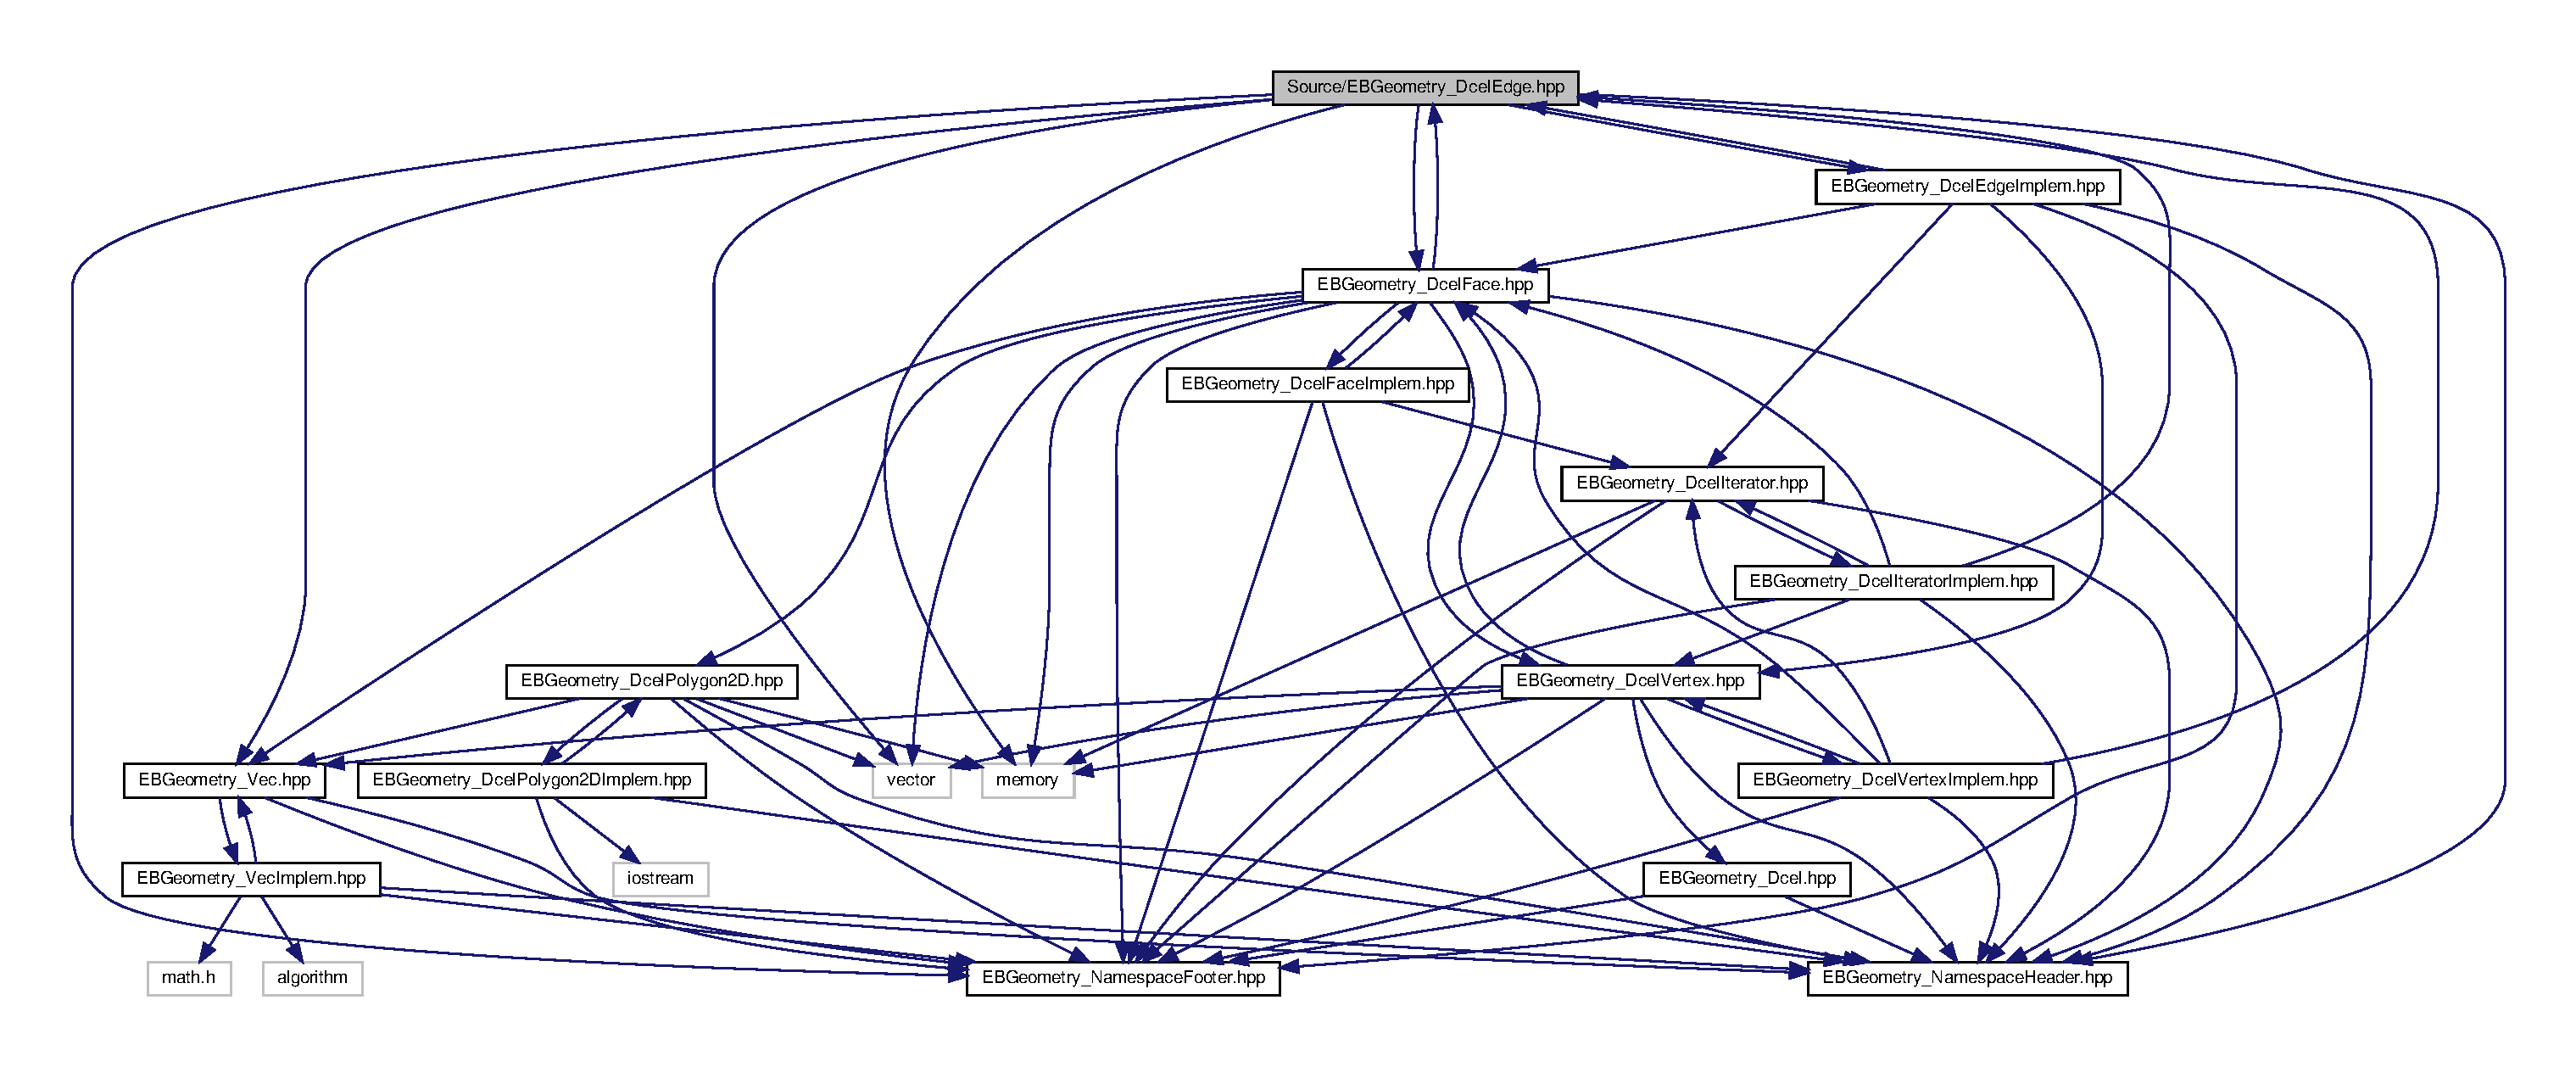
\includegraphics[width=350pt]{EBGeometry__DcelEdge_8hpp__incl}
\end{center}
\end{figure}
This graph shows which files directly or indirectly include this file\+:
\nopagebreak
\begin{figure}[H]
\begin{center}
\leavevmode
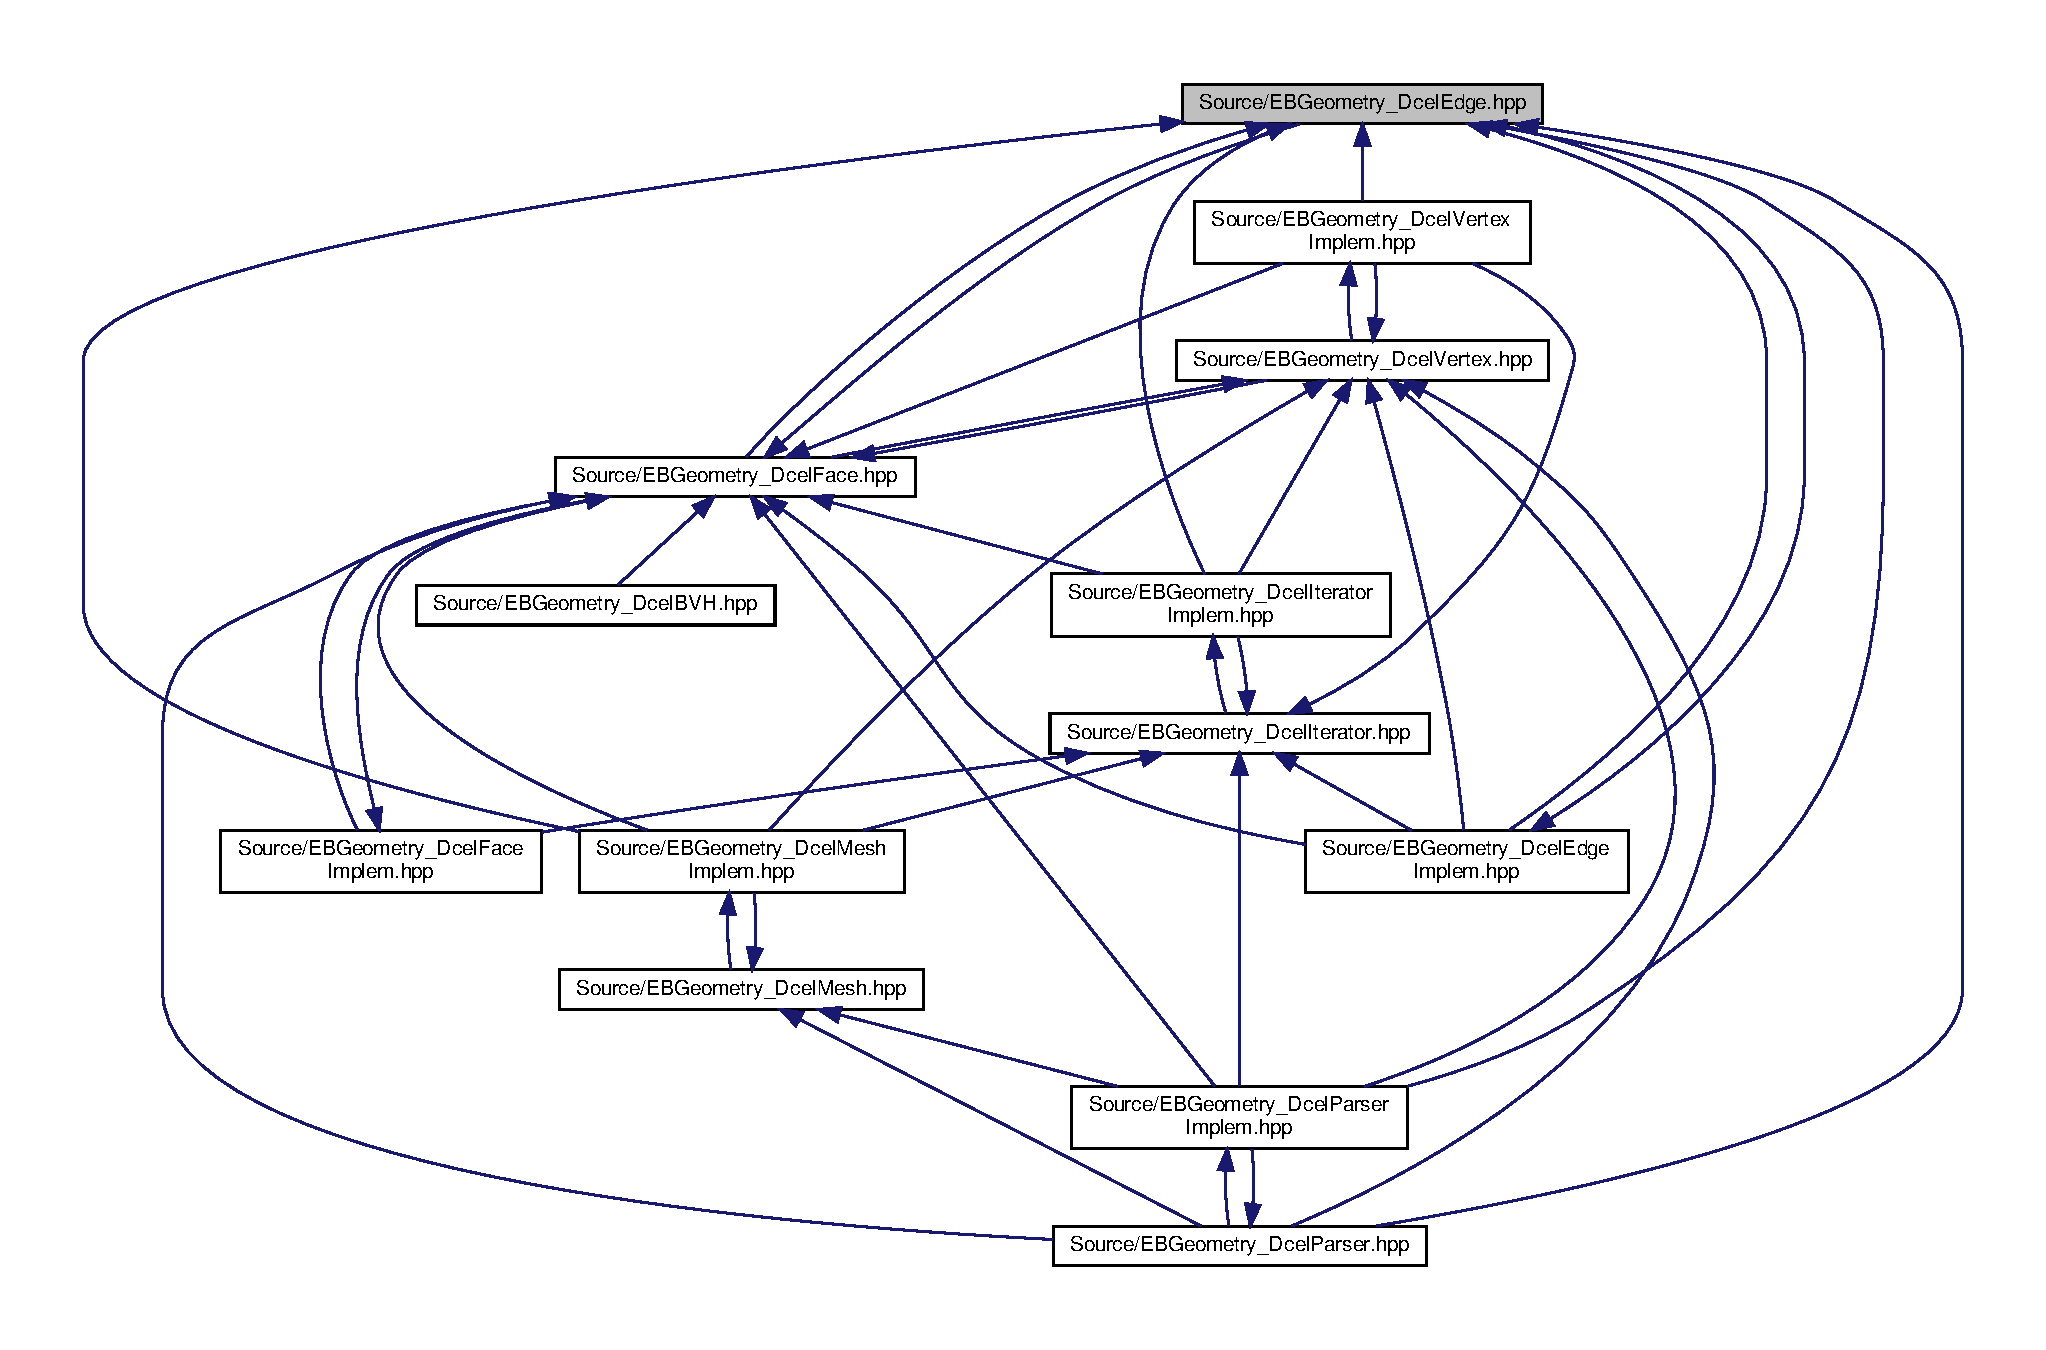
\includegraphics[width=350pt]{EBGeometry__DcelEdge_8hpp__dep__incl}
\end{center}
\end{figure}
\doxysubsection*{Classes}
\begin{DoxyCompactItemize}
\item 
class \mbox{\hyperlink{classDcel_1_1VertexT}{Dcel\+::\+Vertex\+T$<$ T $>$}}
\begin{DoxyCompactList}\small\item\em Class which represents a vertex node in a double-\/edge connected list (D\+C\+EL). \end{DoxyCompactList}\item 
class \mbox{\hyperlink{classDcel_1_1EdgeT}{Dcel\+::\+Edge\+T$<$ T $>$}}
\begin{DoxyCompactList}\small\item\em Class which represents a half-\/edge in a double-\/edge connected list (D\+C\+EL). \end{DoxyCompactList}\item 
class \mbox{\hyperlink{classDcel_1_1FaceT}{Dcel\+::\+Face\+T$<$ T $>$}}
\begin{DoxyCompactList}\small\item\em Class which represents a polygon face in a double-\/edge connected list (D\+C\+EL). \end{DoxyCompactList}\item 
class \mbox{\hyperlink{classDcel_1_1EdgeIteratorT}{Dcel\+::\+Edge\+Iterator\+T$<$ T $>$}}
\begin{DoxyCompactList}\small\item\em Class which can iterate through edges and vertices around a D\+C\+EL polygon face. \end{DoxyCompactList}\item 
class \mbox{\hyperlink{classDcel_1_1EdgeT}{Dcel\+::\+Edge\+T$<$ T $>$}}
\begin{DoxyCompactList}\small\item\em Class which represents a half-\/edge in a double-\/edge connected list (D\+C\+EL). \end{DoxyCompactList}\end{DoxyCompactItemize}
\doxysubsection*{Namespaces}
\begin{DoxyCompactItemize}
\item 
 \mbox{\hyperlink{namespaceDcel}{Dcel}}
\begin{DoxyCompactList}\small\item\em Namespace containing various double-\/connected edge list (D\+C\+EL) functionality. \end{DoxyCompactList}\end{DoxyCompactItemize}


\doxysubsection{Detailed Description}
Declaration of a half-\/edge class for use in D\+C\+EL descriptions of polygon tesselations. 

\begin{DoxyAuthor}{Author}
Robert Marskar 
\end{DoxyAuthor}

\hypertarget{EBGeometry__DcelEdgeImplem_8hpp}{}\section{Source/\+E\+B\+Geometry\+\_\+\+Dcel\+Edge\+Implem.hpp File Reference}
\label{EBGeometry__DcelEdgeImplem_8hpp}\index{Source/\+E\+B\+Geometry\+\_\+\+Dcel\+Edge\+Implem.\+hpp@{Source/\+E\+B\+Geometry\+\_\+\+Dcel\+Edge\+Implem.\+hpp}}


Implementation of \hyperlink{EBGeometry__DcelEdge_8hpp}{E\+B\+Geometry\+\_\+\+Dcel\+Edge.\+hpp}.  


{\ttfamily \#include \char`\"{}E\+B\+Geometry\+\_\+\+Dcel\+Vertex.\+hpp\char`\"{}}\newline
{\ttfamily \#include \char`\"{}E\+B\+Geometry\+\_\+\+Dcel\+Edge.\+hpp\char`\"{}}\newline
{\ttfamily \#include \char`\"{}E\+B\+Geometry\+\_\+\+Dcel\+Face.\+hpp\char`\"{}}\newline
{\ttfamily \#include \char`\"{}E\+B\+Geometry\+\_\+\+Dcel\+Iterator.\+hpp\char`\"{}}\newline
{\ttfamily \#include \char`\"{}E\+B\+Geometry\+\_\+\+Namespace\+Header.\+hpp\char`\"{}}\newline
{\ttfamily \#include \char`\"{}E\+B\+Geometry\+\_\+\+Namespace\+Footer.\+hpp\char`\"{}}\newline
Include dependency graph for E\+B\+Geometry\+\_\+\+Dcel\+Edge\+Implem.\+hpp\+:\nopagebreak
\begin{figure}[H]
\begin{center}
\leavevmode
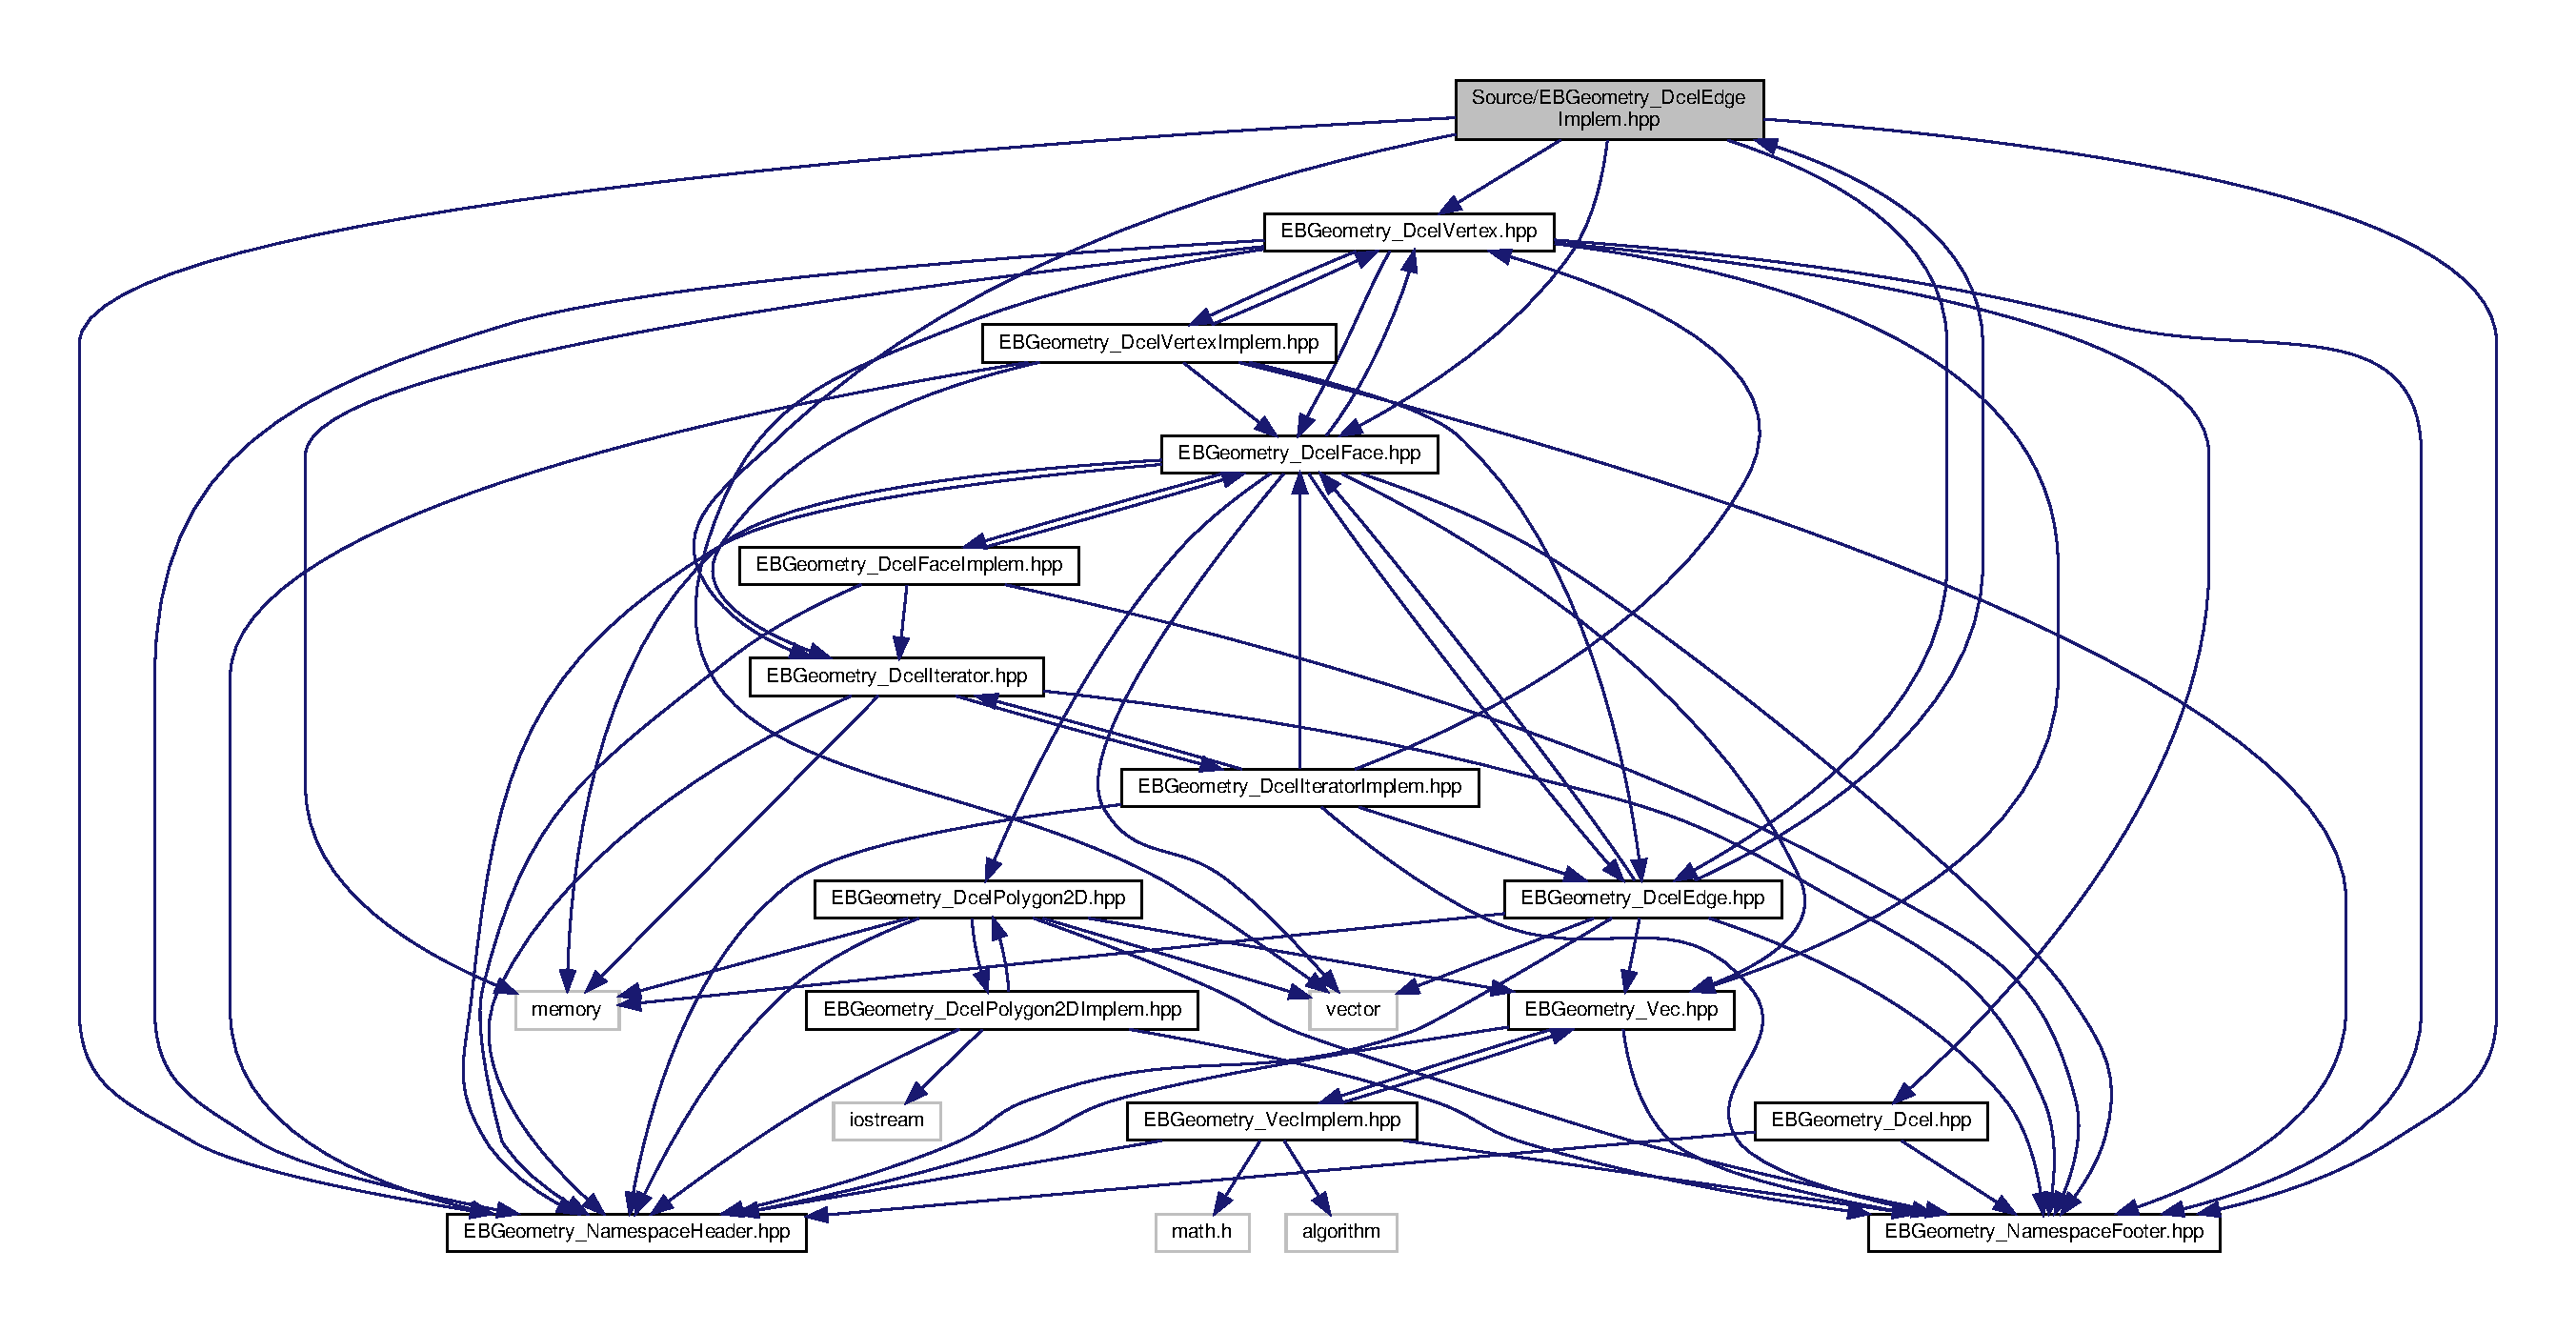
\includegraphics[width=350pt]{EBGeometry__DcelEdgeImplem_8hpp__incl}
\end{center}
\end{figure}
This graph shows which files directly or indirectly include this file\+:\nopagebreak
\begin{figure}[H]
\begin{center}
\leavevmode
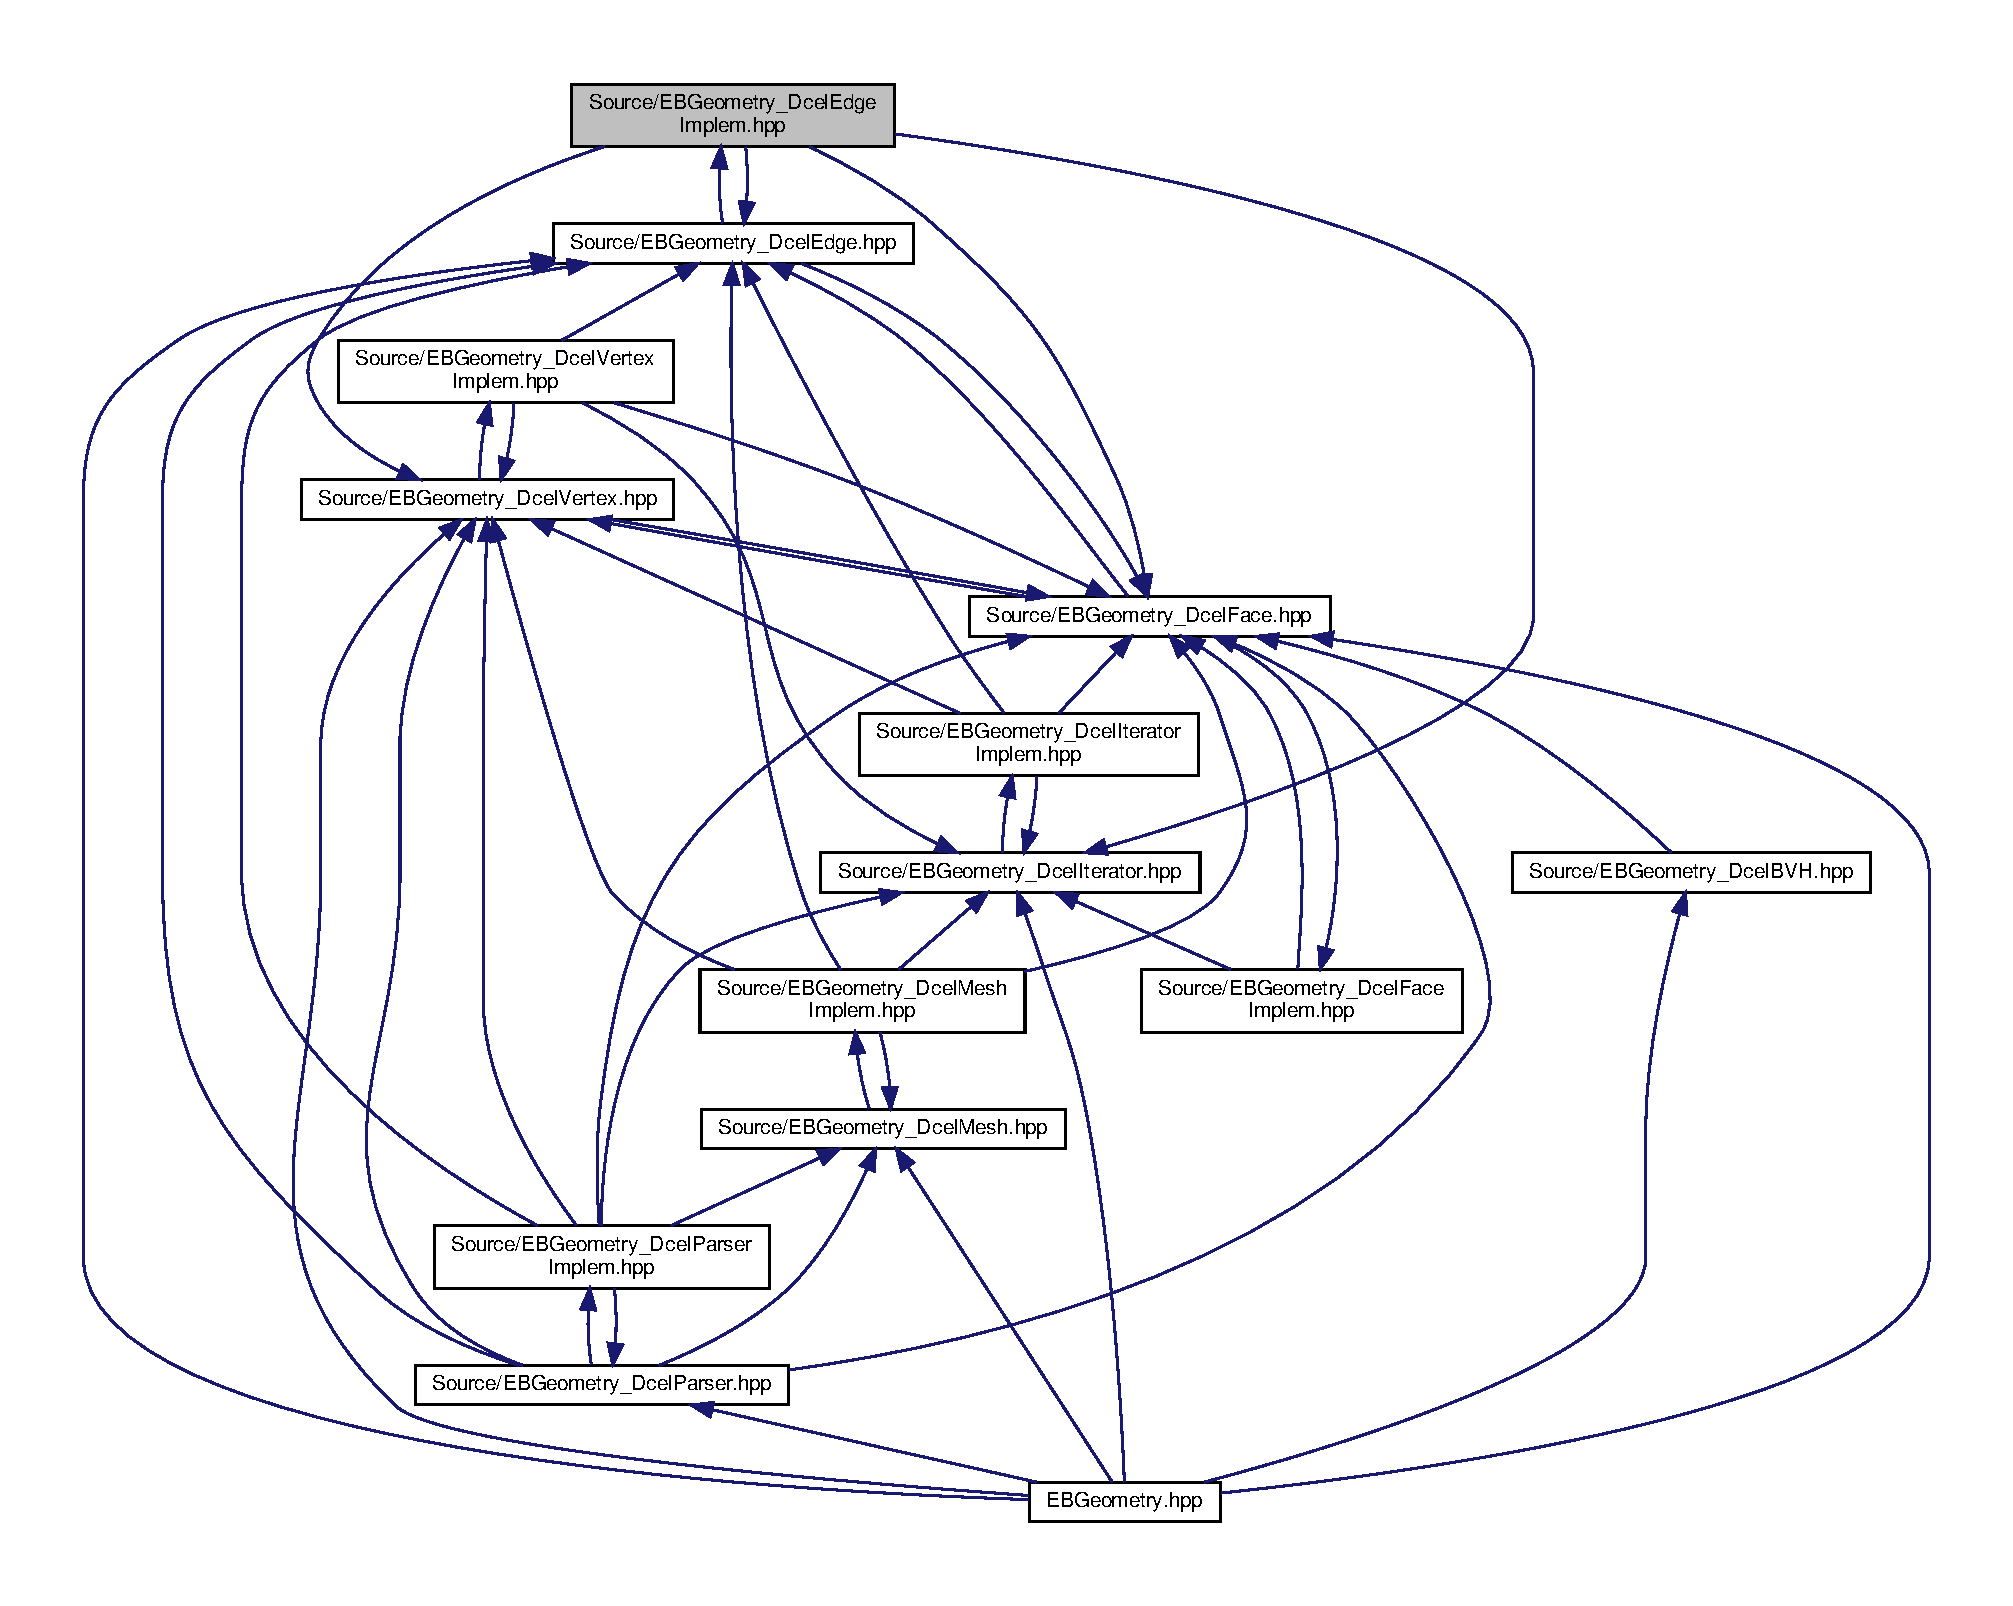
\includegraphics[width=350pt]{EBGeometry__DcelEdgeImplem_8hpp__dep__incl}
\end{center}
\end{figure}
\subsection*{Namespaces}
\begin{DoxyCompactItemize}
\item 
 \hyperlink{namespaceDcel}{Dcel}
\begin{DoxyCompactList}\small\item\em Namespace containing various double-\/connected edge list (D\+C\+EL) functionality. \end{DoxyCompactList}\end{DoxyCompactItemize}


\subsection{Detailed Description}
Implementation of \hyperlink{EBGeometry__DcelEdge_8hpp}{E\+B\+Geometry\+\_\+\+Dcel\+Edge.\+hpp}. 

\begin{DoxyAuthor}{Author}
Robert Marskar 
\end{DoxyAuthor}
\begin{DoxyRefDesc}{Todo}
\item[\hyperlink{todo__todo000002}{Todo}]Include m\+\_\+face in constructors \end{DoxyRefDesc}

\hypertarget{EBGeometry__DcelFace_8hpp}{}\section{Source/\+E\+B\+Geometry\+\_\+\+Dcel\+Face.hpp File Reference}
\label{EBGeometry__DcelFace_8hpp}\index{Source/\+E\+B\+Geometry\+\_\+\+Dcel\+Face.\+hpp@{Source/\+E\+B\+Geometry\+\_\+\+Dcel\+Face.\+hpp}}


Declaration of a polygon face class for use in D\+C\+EL descriptions of polygon tesselations.  


{\ttfamily \#include $<$memory$>$}\newline
{\ttfamily \#include $<$vector$>$}\newline
{\ttfamily \#include \char`\"{}E\+B\+Geometry\+\_\+\+Vec.\+hpp\char`\"{}}\newline
{\ttfamily \#include \char`\"{}E\+B\+Geometry\+\_\+\+Dcel\+Vertex.\+hpp\char`\"{}}\newline
{\ttfamily \#include \char`\"{}E\+B\+Geometry\+\_\+\+Dcel\+Edge.\+hpp\char`\"{}}\newline
{\ttfamily \#include \char`\"{}E\+B\+Geometry\+\_\+\+Dcel\+Polygon2\+D.\+hpp\char`\"{}}\newline
{\ttfamily \#include \char`\"{}E\+B\+Geometry\+\_\+\+Namespace\+Header.\+hpp\char`\"{}}\newline
{\ttfamily \#include \char`\"{}E\+B\+Geometry\+\_\+\+Namespace\+Footer.\+hpp\char`\"{}}\newline
{\ttfamily \#include \char`\"{}E\+B\+Geometry\+\_\+\+Dcel\+Face\+Implem.\+hpp\char`\"{}}\newline
Include dependency graph for E\+B\+Geometry\+\_\+\+Dcel\+Face.\+hpp\+:\nopagebreak
\begin{figure}[H]
\begin{center}
\leavevmode
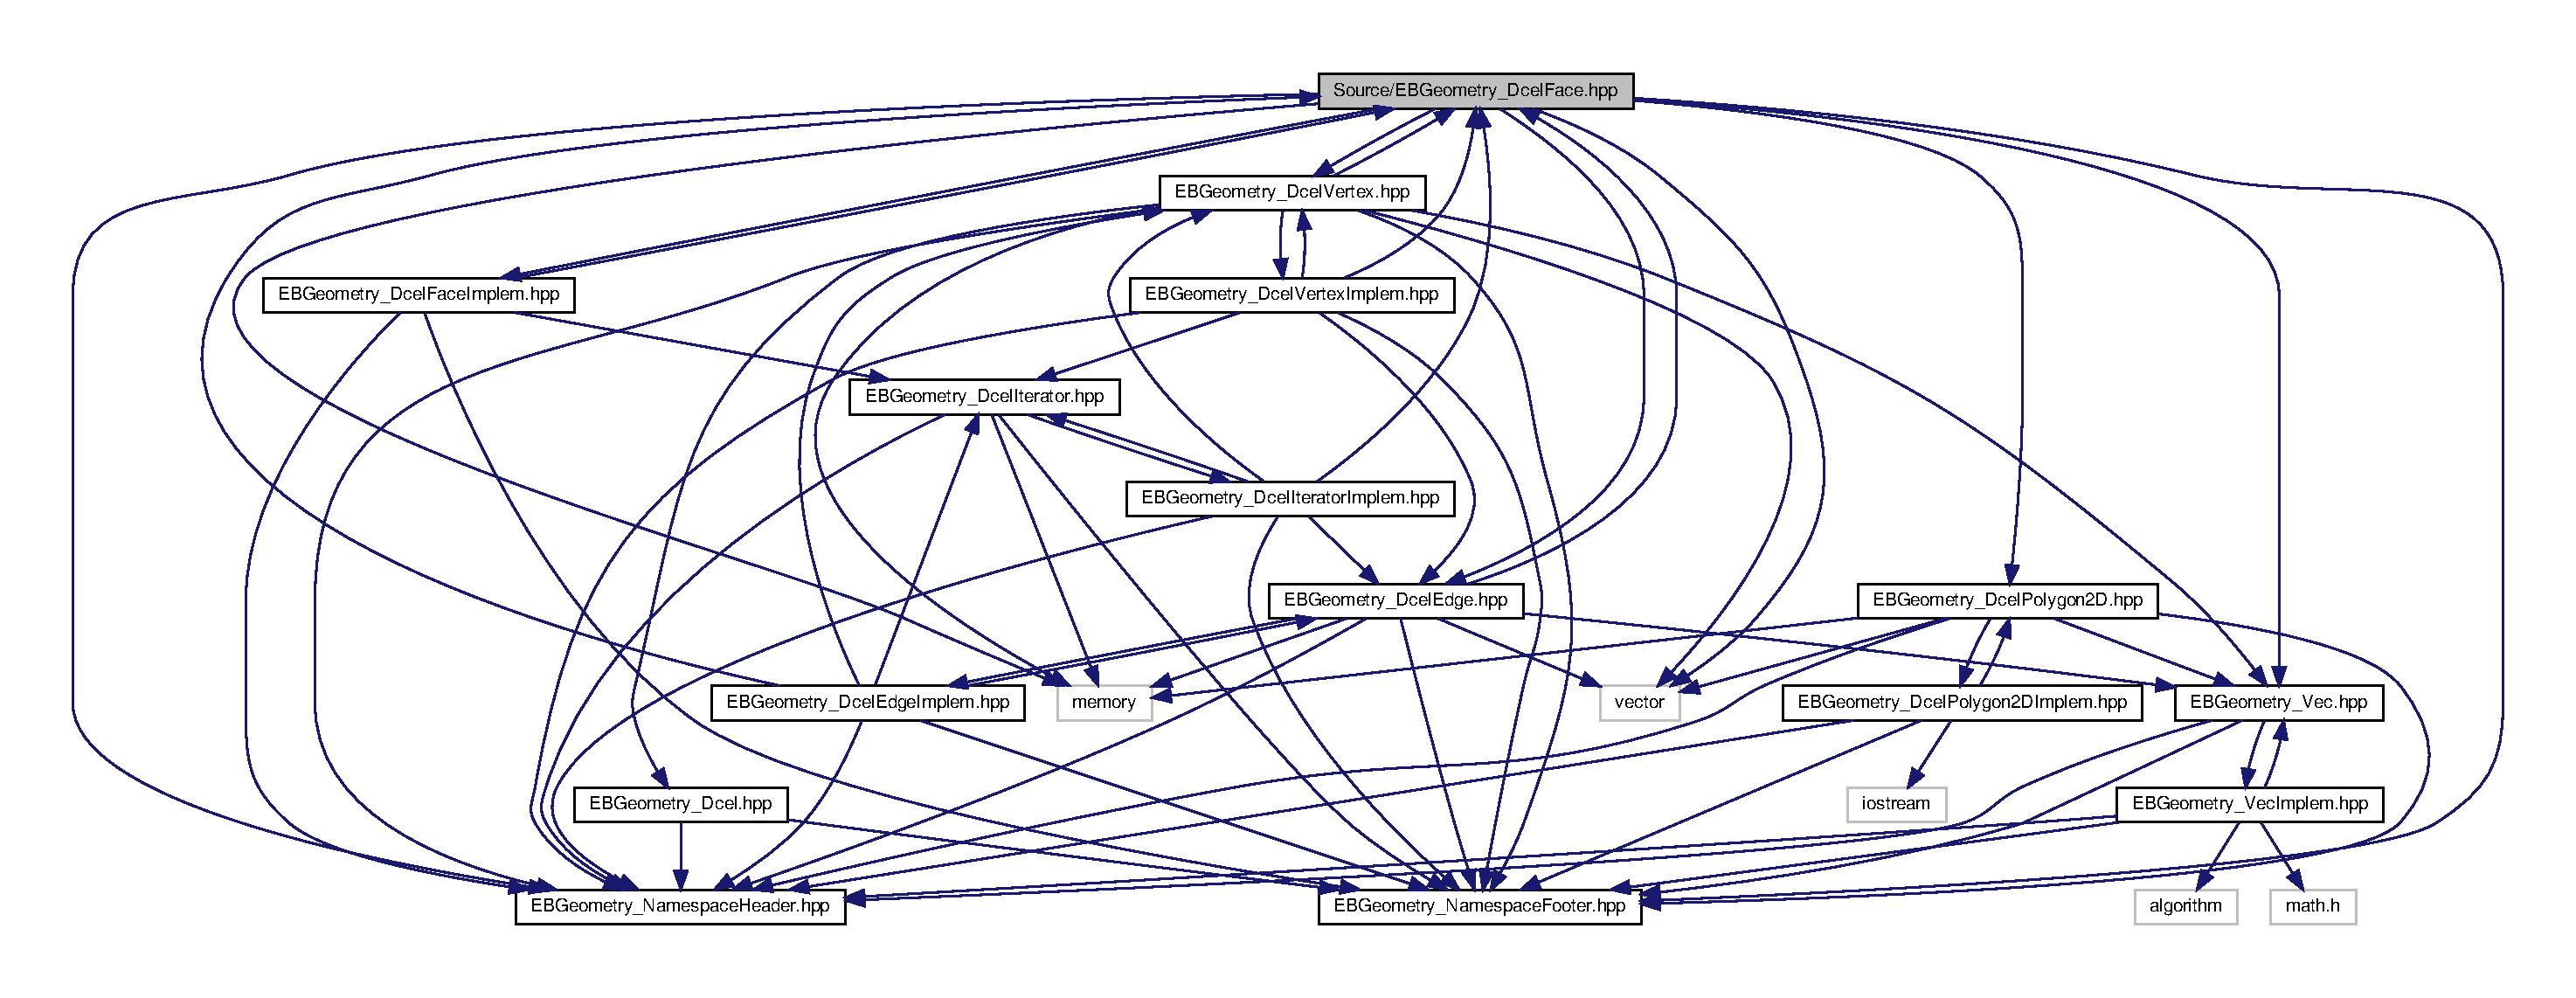
\includegraphics[width=350pt]{EBGeometry__DcelFace_8hpp__incl}
\end{center}
\end{figure}
This graph shows which files directly or indirectly include this file\+:\nopagebreak
\begin{figure}[H]
\begin{center}
\leavevmode
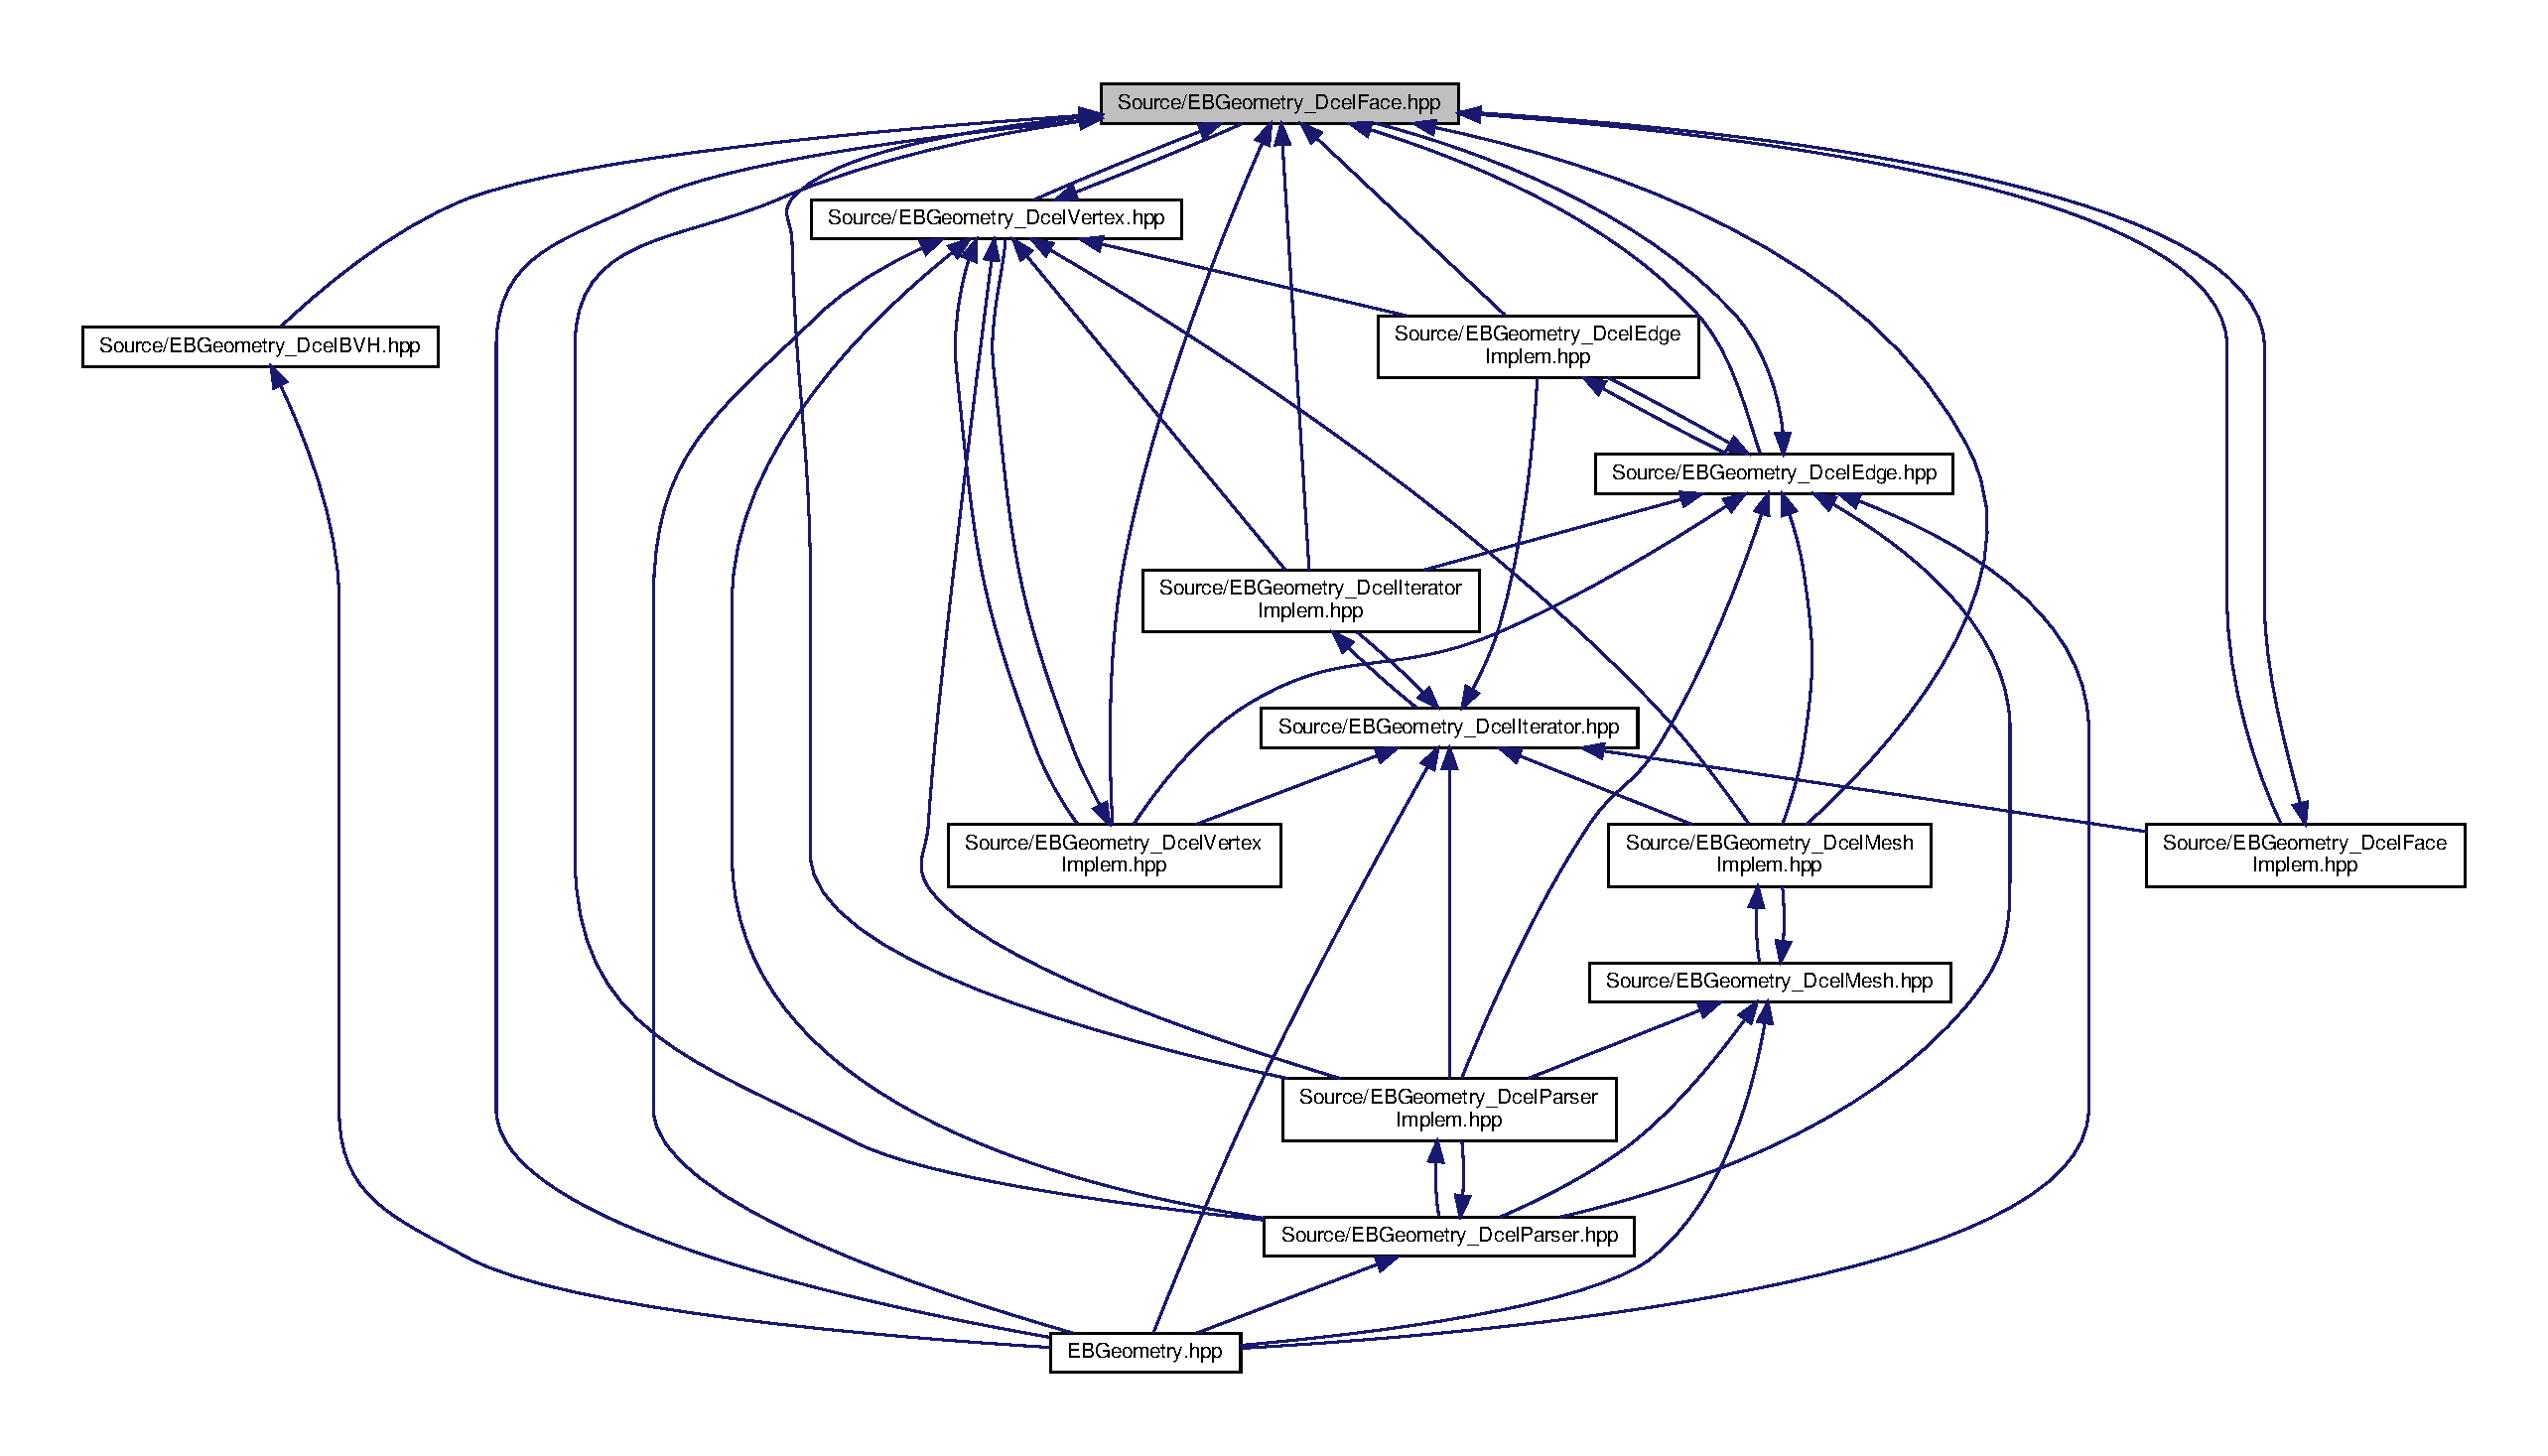
\includegraphics[width=350pt]{EBGeometry__DcelFace_8hpp__dep__incl}
\end{center}
\end{figure}
\subsection*{Classes}
\begin{DoxyCompactItemize}
\item 
class \hyperlink{classDcel_1_1VertexT}{Dcel\+::\+Vertex\+T$<$ T $>$}
\begin{DoxyCompactList}\small\item\em Class which represents a vertex node in a double-\/edge connected list (D\+C\+EL). \end{DoxyCompactList}\item 
class \hyperlink{classDcel_1_1EdgeT}{Dcel\+::\+Edge\+T$<$ T $>$}
\begin{DoxyCompactList}\small\item\em Class which represents a half-\/edge in a double-\/edge connected list (D\+C\+EL). \end{DoxyCompactList}\item 
class \hyperlink{classDcel_1_1FaceT}{Dcel\+::\+Face\+T$<$ T $>$}
\begin{DoxyCompactList}\small\item\em Class which represents a polygon face in a double-\/edge connected list (D\+C\+EL). \end{DoxyCompactList}\item 
class \hyperlink{classDcel_1_1EdgeIteratorT}{Dcel\+::\+Edge\+Iterator\+T$<$ T $>$}
\begin{DoxyCompactList}\small\item\em Class which can iterate through edges and vertices around a D\+C\+EL polygon face. \end{DoxyCompactList}\item 
class \hyperlink{classDcel_1_1FaceT}{Dcel\+::\+Face\+T$<$ T $>$}
\begin{DoxyCompactList}\small\item\em Class which represents a polygon face in a double-\/edge connected list (D\+C\+EL). \end{DoxyCompactList}\end{DoxyCompactItemize}
\subsection*{Namespaces}
\begin{DoxyCompactItemize}
\item 
 \hyperlink{namespaceDcel}{Dcel}
\begin{DoxyCompactList}\small\item\em Namespace containing various double-\/connected edge list (D\+C\+EL) functionality. \end{DoxyCompactList}\end{DoxyCompactItemize}


\subsection{Detailed Description}
Declaration of a polygon face class for use in D\+C\+EL descriptions of polygon tesselations. 

\begin{DoxyAuthor}{Author}
Robert Marskar 
\end{DoxyAuthor}

\hypertarget{EBGeometry__DcelFaceImplem_8hpp}{}\section{Source/\+E\+B\+Geometry\+\_\+\+Dcel\+Face\+Implem.hpp File Reference}
\label{EBGeometry__DcelFaceImplem_8hpp}\index{Source/\+E\+B\+Geometry\+\_\+\+Dcel\+Face\+Implem.\+hpp@{Source/\+E\+B\+Geometry\+\_\+\+Dcel\+Face\+Implem.\+hpp}}


Implementation of \hyperlink{EBGeometry__DcelFace_8hpp}{E\+B\+Geometry\+\_\+\+Dcel\+Face.\+hpp}.  


{\ttfamily \#include \char`\"{}E\+B\+Geometry\+\_\+\+Dcel\+Face.\+hpp\char`\"{}}\newline
{\ttfamily \#include \char`\"{}E\+B\+Geometry\+\_\+\+Dcel\+Iterator.\+hpp\char`\"{}}\newline
{\ttfamily \#include \char`\"{}E\+B\+Geometry\+\_\+\+Namespace\+Header.\+hpp\char`\"{}}\newline
{\ttfamily \#include \char`\"{}E\+B\+Geometry\+\_\+\+Namespace\+Footer.\+hpp\char`\"{}}\newline
Include dependency graph for E\+B\+Geometry\+\_\+\+Dcel\+Face\+Implem.\+hpp\+:\nopagebreak
\begin{figure}[H]
\begin{center}
\leavevmode
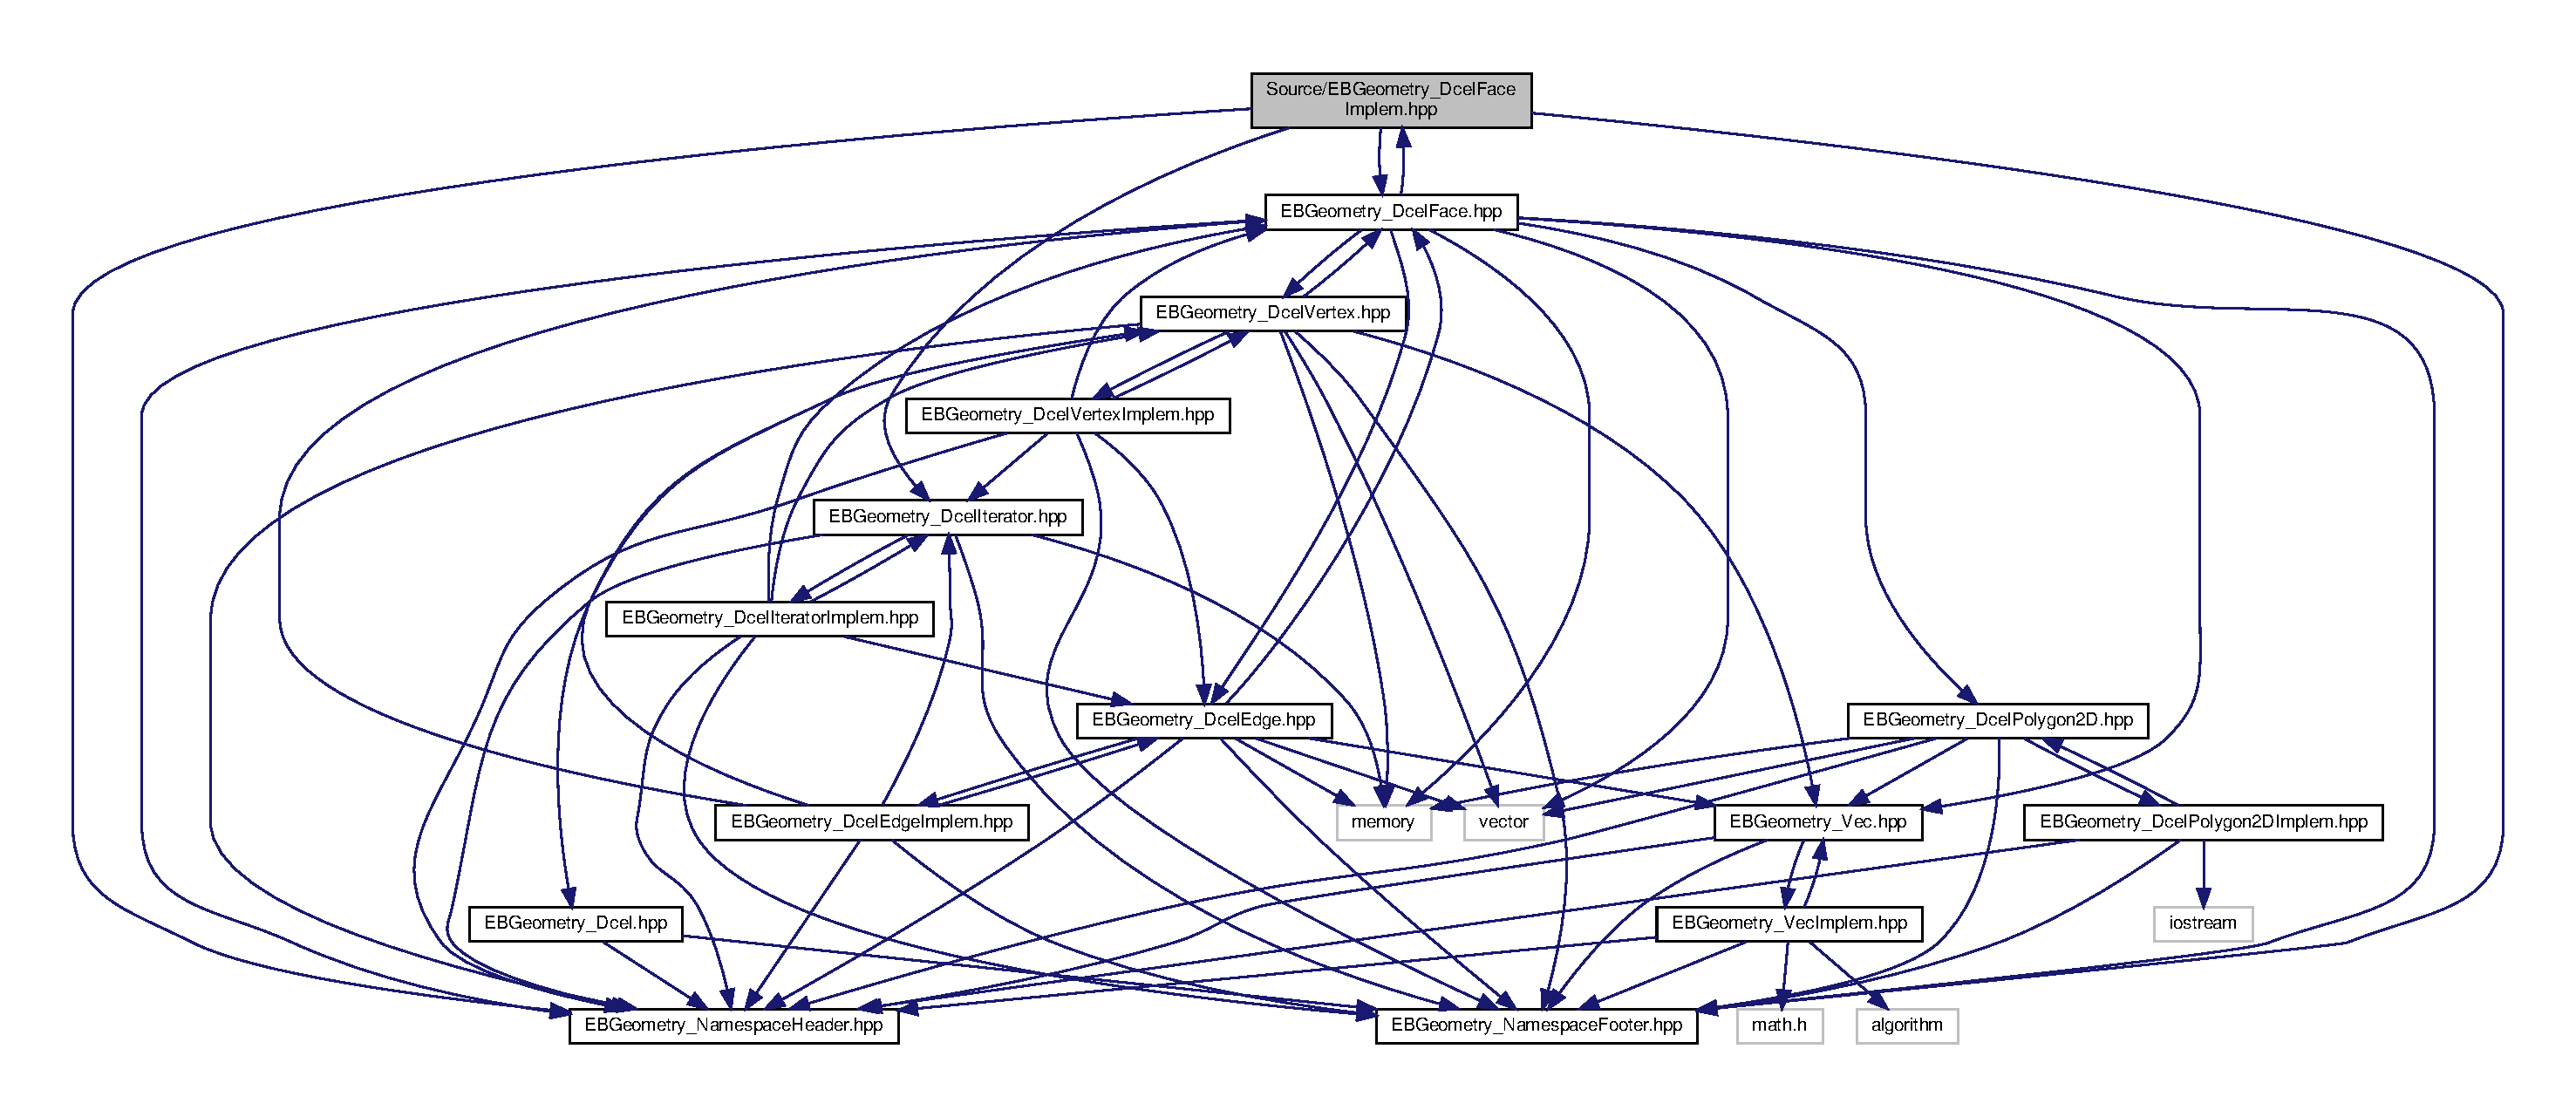
\includegraphics[width=350pt]{EBGeometry__DcelFaceImplem_8hpp__incl}
\end{center}
\end{figure}
This graph shows which files directly or indirectly include this file\+:\nopagebreak
\begin{figure}[H]
\begin{center}
\leavevmode
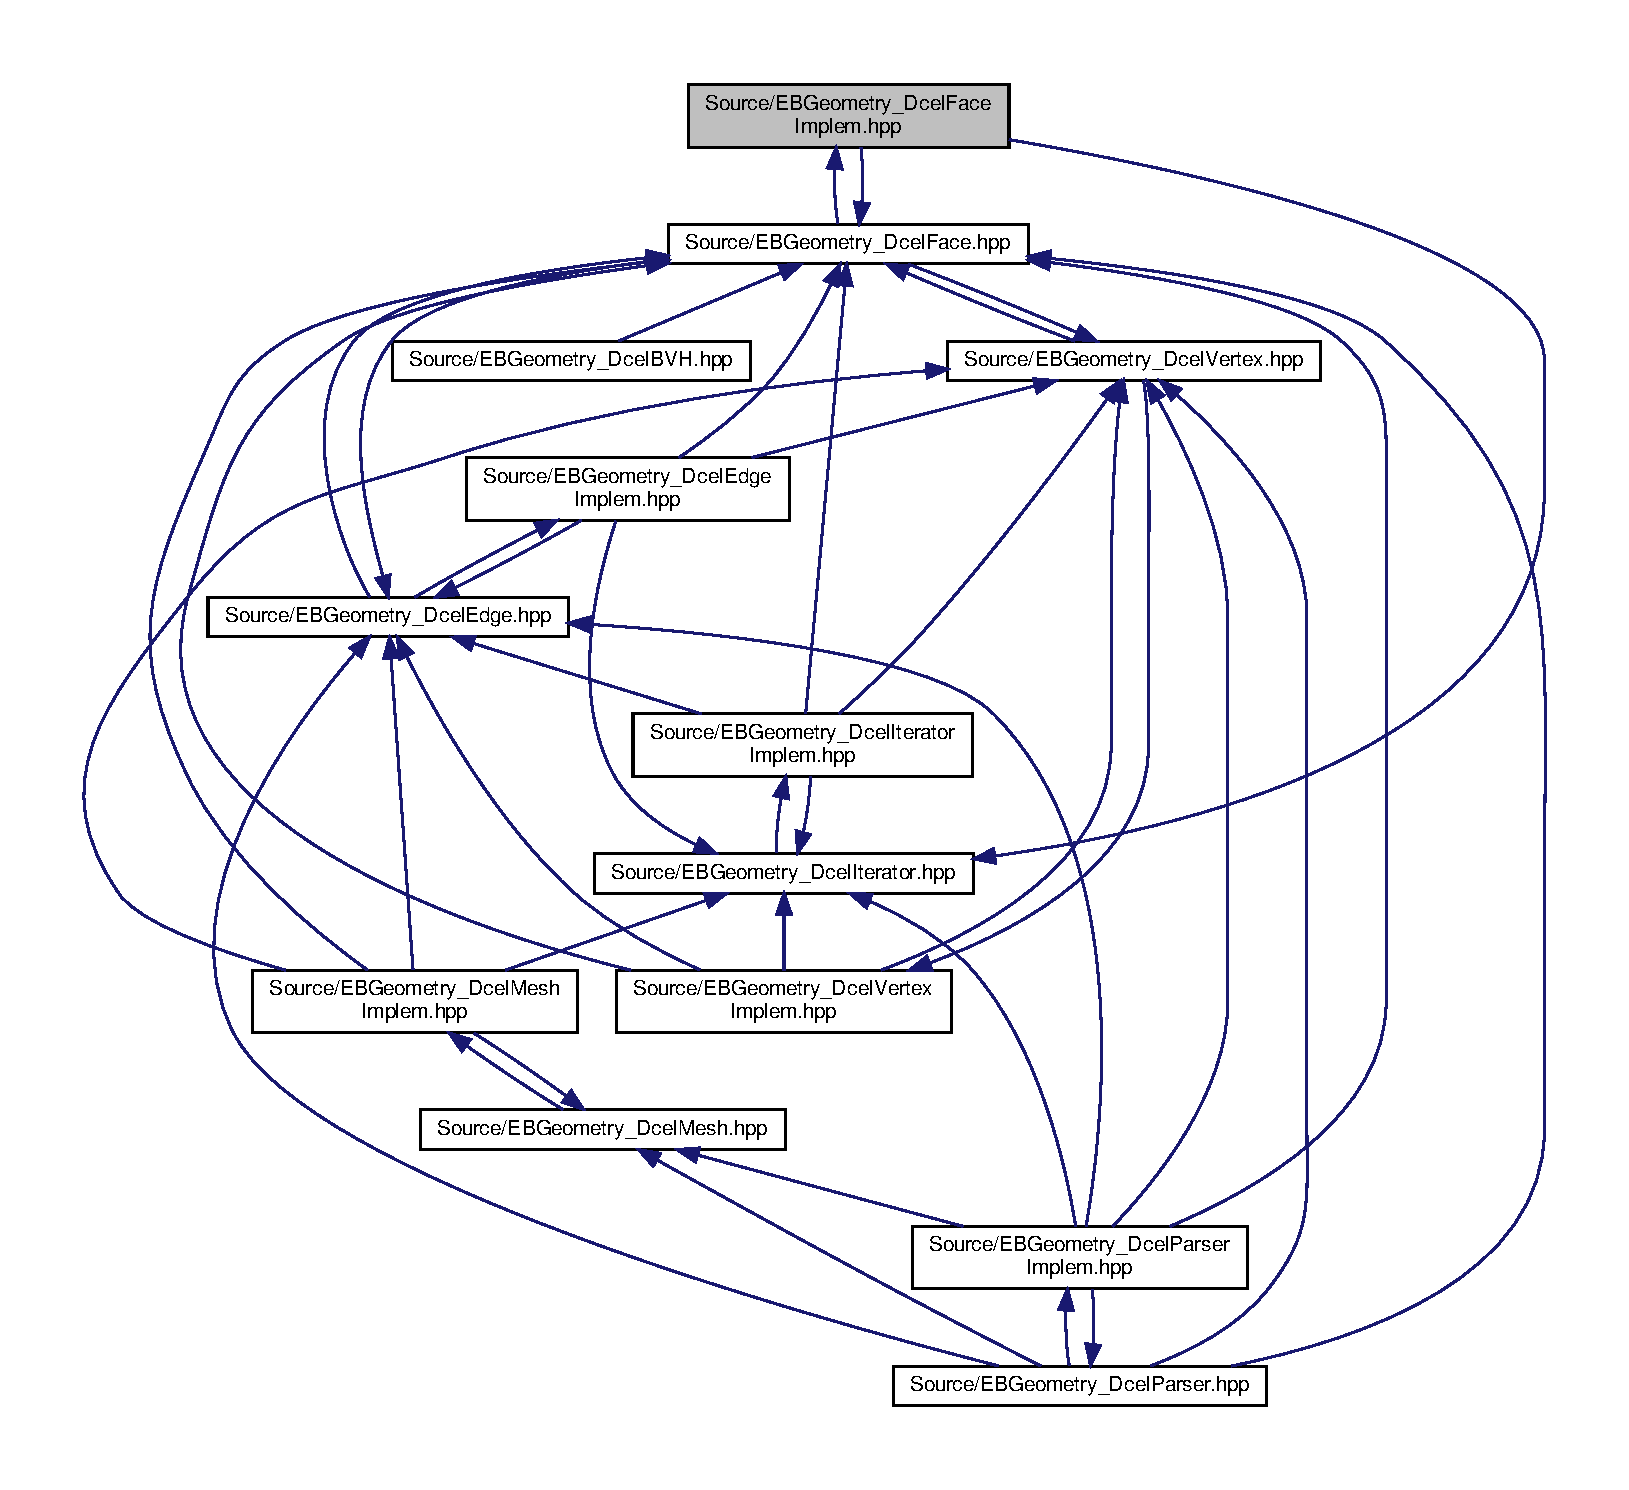
\includegraphics[width=350pt]{EBGeometry__DcelFaceImplem_8hpp__dep__incl}
\end{center}
\end{figure}
\subsection*{Namespaces}
\begin{DoxyCompactItemize}
\item 
 \hyperlink{namespaceDcel}{Dcel}
\begin{DoxyCompactList}\small\item\em Namespace containing various double-\/connected edge list (D\+C\+EL) functionality. \end{DoxyCompactList}\end{DoxyCompactItemize}


\subsection{Detailed Description}
Implementation of \hyperlink{EBGeometry__DcelFace_8hpp}{E\+B\+Geometry\+\_\+\+Dcel\+Face.\+hpp}. 

\begin{DoxyAuthor}{Author}
Robert Marskar 
\end{DoxyAuthor}

\hypertarget{EBGeometry__DcelIterator_8hpp}{}\section{Source/\+E\+B\+Geometry\+\_\+\+Dcel\+Iterator.hpp File Reference}
\label{EBGeometry__DcelIterator_8hpp}\index{Source/\+E\+B\+Geometry\+\_\+\+Dcel\+Iterator.\+hpp@{Source/\+E\+B\+Geometry\+\_\+\+Dcel\+Iterator.\+hpp}}


Declaration of iterators for D\+C\+EL surface Tesselations.  


{\ttfamily \#include $<$memory$>$}\newline
{\ttfamily \#include \char`\"{}E\+B\+Geometry\+\_\+\+Namespace\+Header.\+hpp\char`\"{}}\newline
{\ttfamily \#include \char`\"{}E\+B\+Geometry\+\_\+\+Namespace\+Footer.\+hpp\char`\"{}}\newline
{\ttfamily \#include \char`\"{}E\+B\+Geometry\+\_\+\+Dcel\+Iterator\+Implem.\+hpp\char`\"{}}\newline
Include dependency graph for E\+B\+Geometry\+\_\+\+Dcel\+Iterator.\+hpp\+:\nopagebreak
\begin{figure}[H]
\begin{center}
\leavevmode
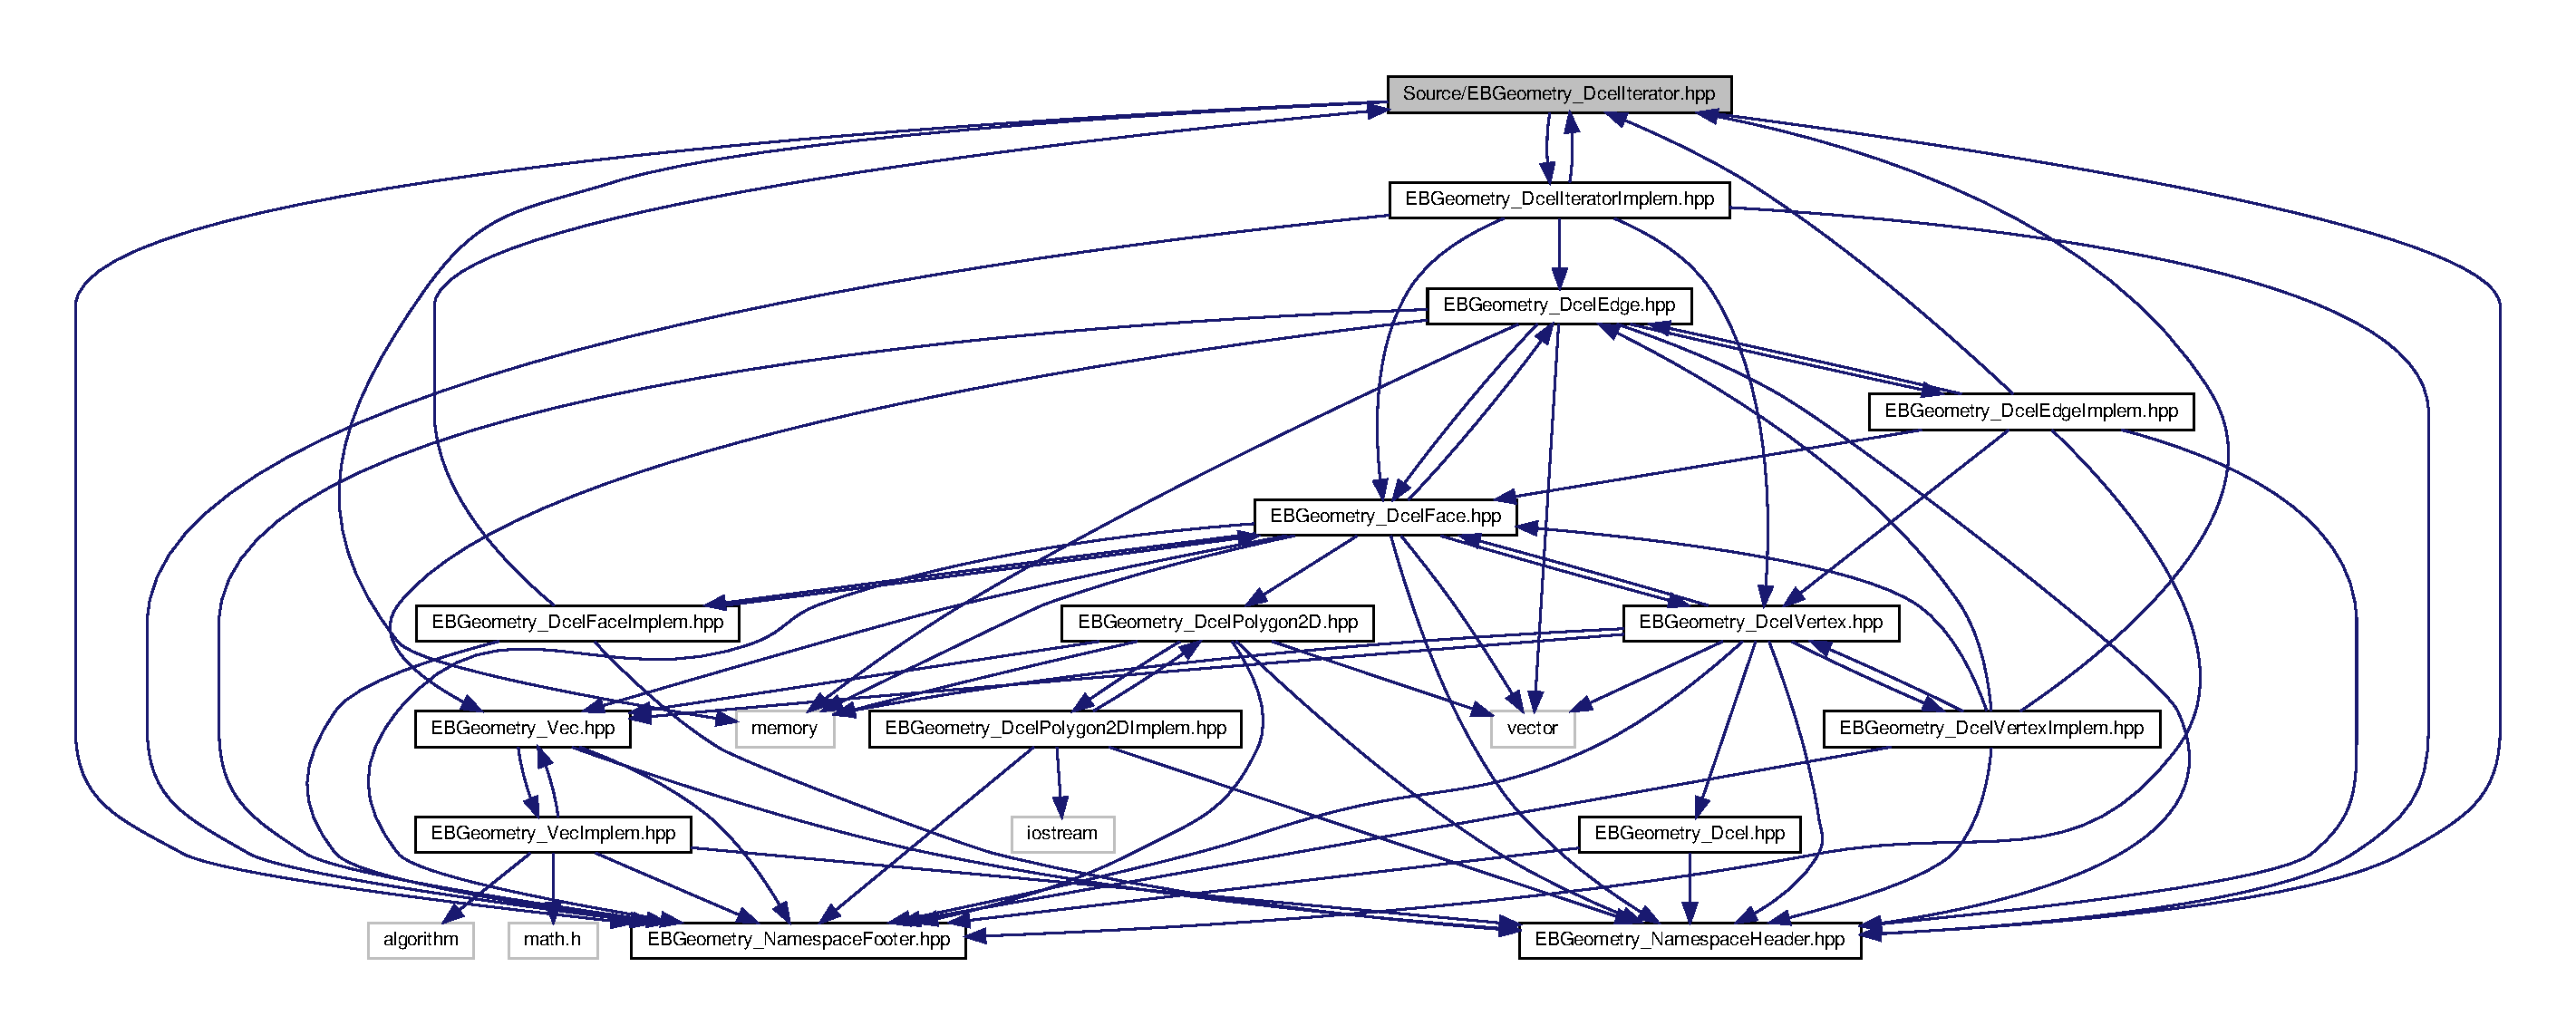
\includegraphics[width=350pt]{EBGeometry__DcelIterator_8hpp__incl}
\end{center}
\end{figure}
This graph shows which files directly or indirectly include this file\+:\nopagebreak
\begin{figure}[H]
\begin{center}
\leavevmode
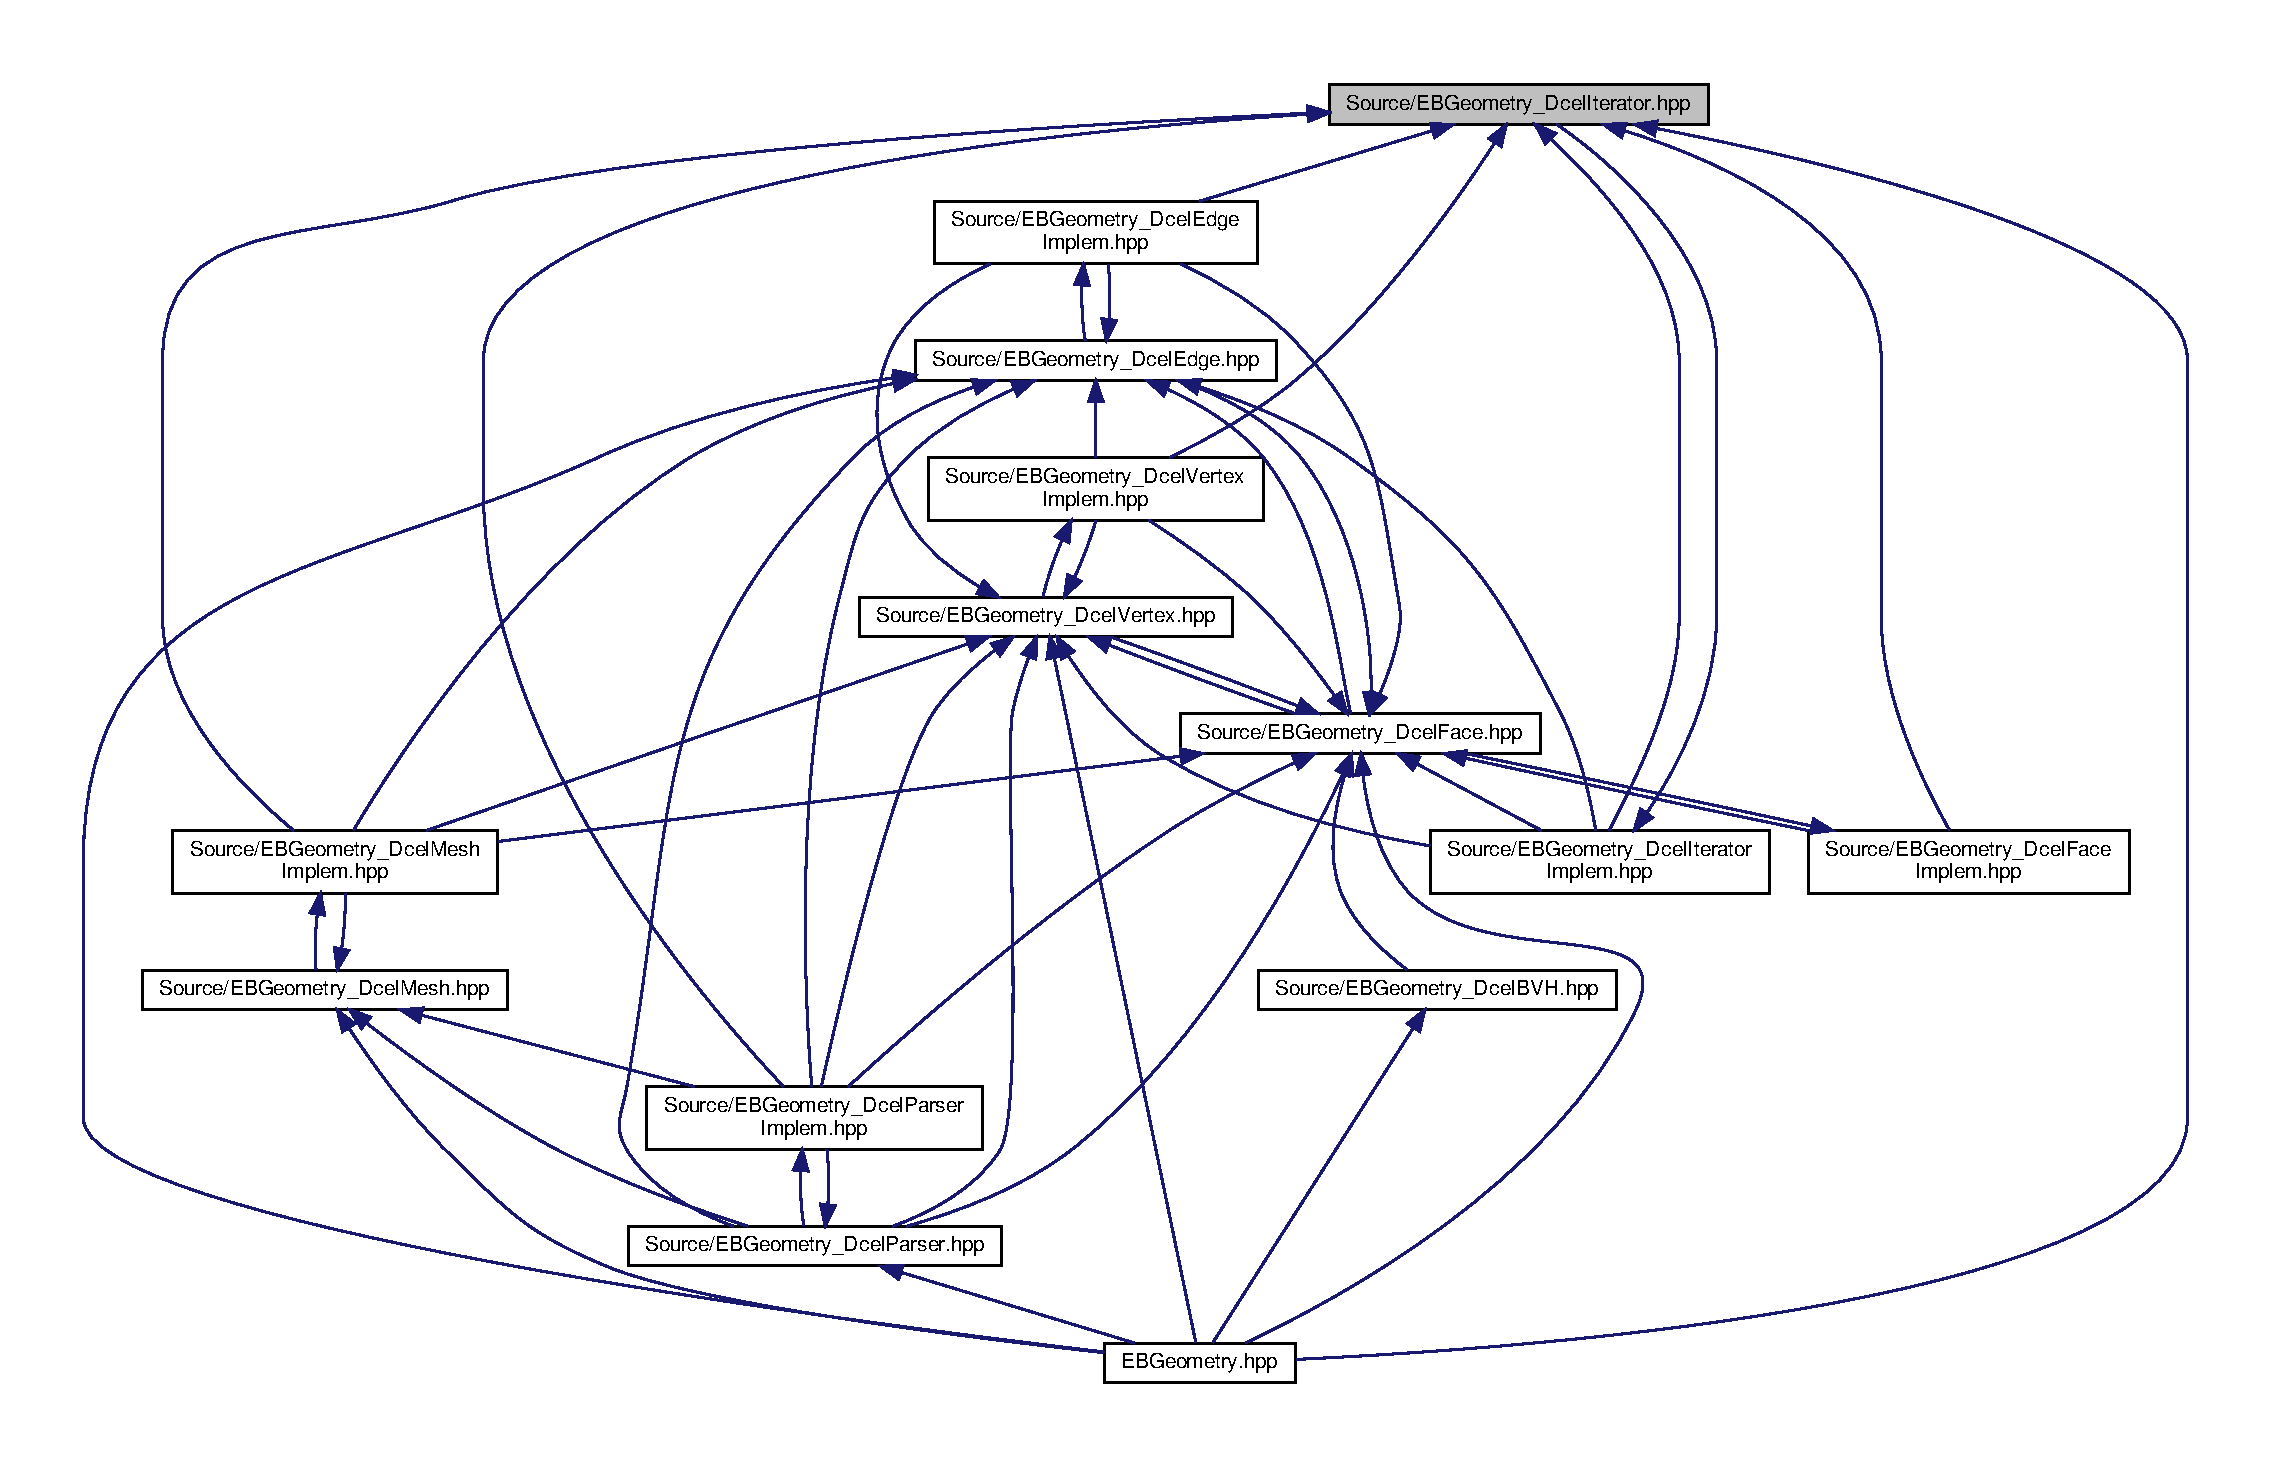
\includegraphics[width=350pt]{EBGeometry__DcelIterator_8hpp__dep__incl}
\end{center}
\end{figure}
\subsection*{Classes}
\begin{DoxyCompactItemize}
\item 
class \hyperlink{classDcel_1_1VertexT}{Dcel\+::\+Vertex\+T$<$ T $>$}
\begin{DoxyCompactList}\small\item\em Class which represents a vertex node in a double-\/edge connected list (D\+C\+EL). \end{DoxyCompactList}\item 
class \hyperlink{classDcel_1_1EdgeT}{Dcel\+::\+Edge\+T$<$ T $>$}
\begin{DoxyCompactList}\small\item\em Class which represents a half-\/edge in a double-\/edge connected list (D\+C\+EL). \end{DoxyCompactList}\item 
class \hyperlink{classDcel_1_1FaceT}{Dcel\+::\+Face\+T$<$ T $>$}
\begin{DoxyCompactList}\small\item\em Class which represents a polygon face in a double-\/edge connected list (D\+C\+EL). \end{DoxyCompactList}\item 
class \hyperlink{classDcel_1_1EdgeIteratorT}{Dcel\+::\+Edge\+Iterator\+T$<$ T $>$}
\begin{DoxyCompactList}\small\item\em Class which can iterate through edges and vertices around a D\+C\+EL polygon face. \end{DoxyCompactList}\end{DoxyCompactItemize}
\subsection*{Namespaces}
\begin{DoxyCompactItemize}
\item 
 \hyperlink{namespaceDcel}{Dcel}
\begin{DoxyCompactList}\small\item\em Namespace containing various double-\/connected edge list (D\+C\+EL) functionality. \end{DoxyCompactList}\end{DoxyCompactItemize}


\subsection{Detailed Description}
Declaration of iterators for D\+C\+EL surface Tesselations. 

\begin{DoxyAuthor}{Author}
Robert Marskar 
\end{DoxyAuthor}

\hypertarget{EBGeometry__DcelIteratorImplem_8hpp}{}\section{Source/\+E\+B\+Geometry\+\_\+\+Dcel\+Iterator\+Implem.hpp File Reference}
\label{EBGeometry__DcelIteratorImplem_8hpp}\index{Source/\+E\+B\+Geometry\+\_\+\+Dcel\+Iterator\+Implem.\+hpp@{Source/\+E\+B\+Geometry\+\_\+\+Dcel\+Iterator\+Implem.\+hpp}}


Implementation of \hyperlink{EBGeometry__DcelIterator_8hpp}{E\+B\+Geometry\+\_\+\+Dcel\+Iterator.\+hpp}.  


{\ttfamily \#include \char`\"{}E\+B\+Geometry\+\_\+\+Dcel\+Vertex.\+hpp\char`\"{}}\newline
{\ttfamily \#include \char`\"{}E\+B\+Geometry\+\_\+\+Dcel\+Edge.\+hpp\char`\"{}}\newline
{\ttfamily \#include \char`\"{}E\+B\+Geometry\+\_\+\+Dcel\+Face.\+hpp\char`\"{}}\newline
{\ttfamily \#include \char`\"{}E\+B\+Geometry\+\_\+\+Dcel\+Iterator.\+hpp\char`\"{}}\newline
{\ttfamily \#include \char`\"{}E\+B\+Geometry\+\_\+\+Namespace\+Header.\+hpp\char`\"{}}\newline
{\ttfamily \#include \char`\"{}E\+B\+Geometry\+\_\+\+Namespace\+Footer.\+hpp\char`\"{}}\newline
Include dependency graph for E\+B\+Geometry\+\_\+\+Dcel\+Iterator\+Implem.\+hpp\+:\nopagebreak
\begin{figure}[H]
\begin{center}
\leavevmode
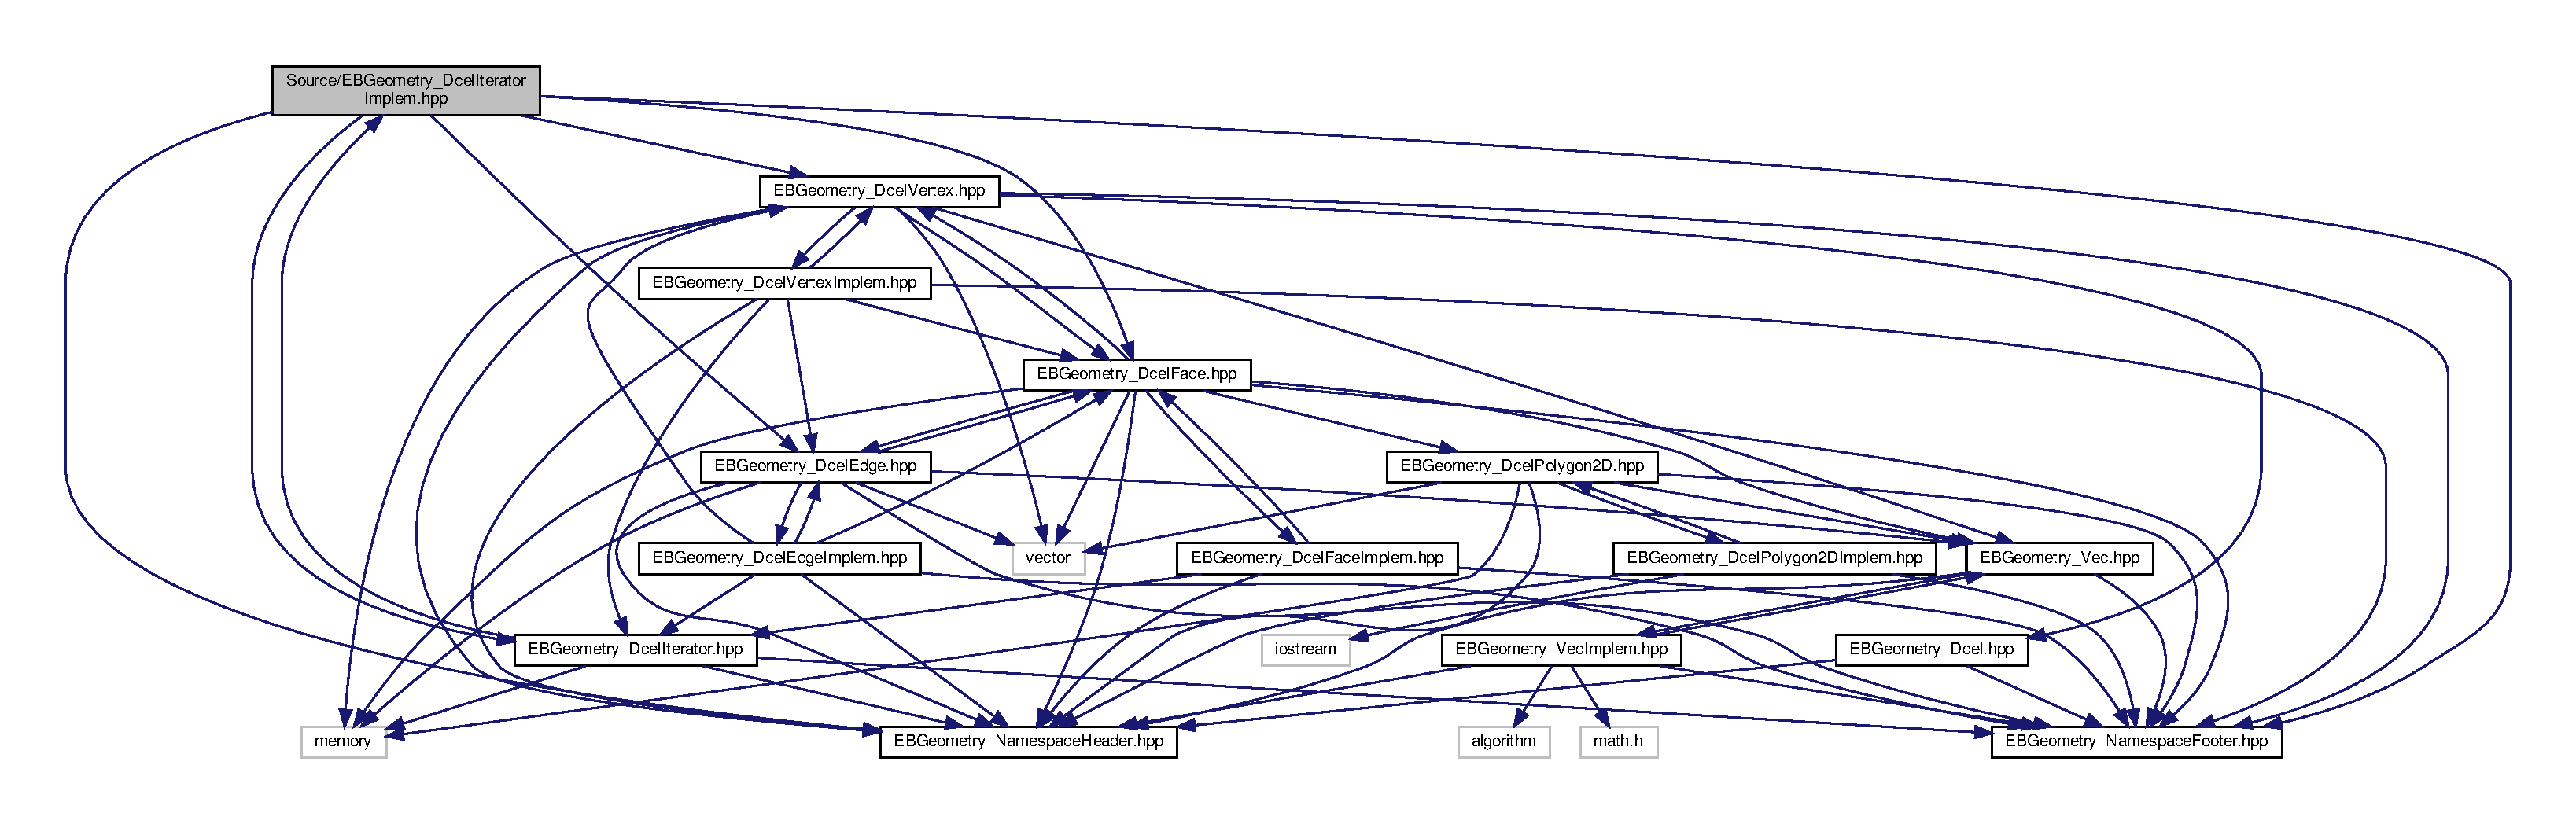
\includegraphics[width=350pt]{EBGeometry__DcelIteratorImplem_8hpp__incl}
\end{center}
\end{figure}
This graph shows which files directly or indirectly include this file\+:\nopagebreak
\begin{figure}[H]
\begin{center}
\leavevmode
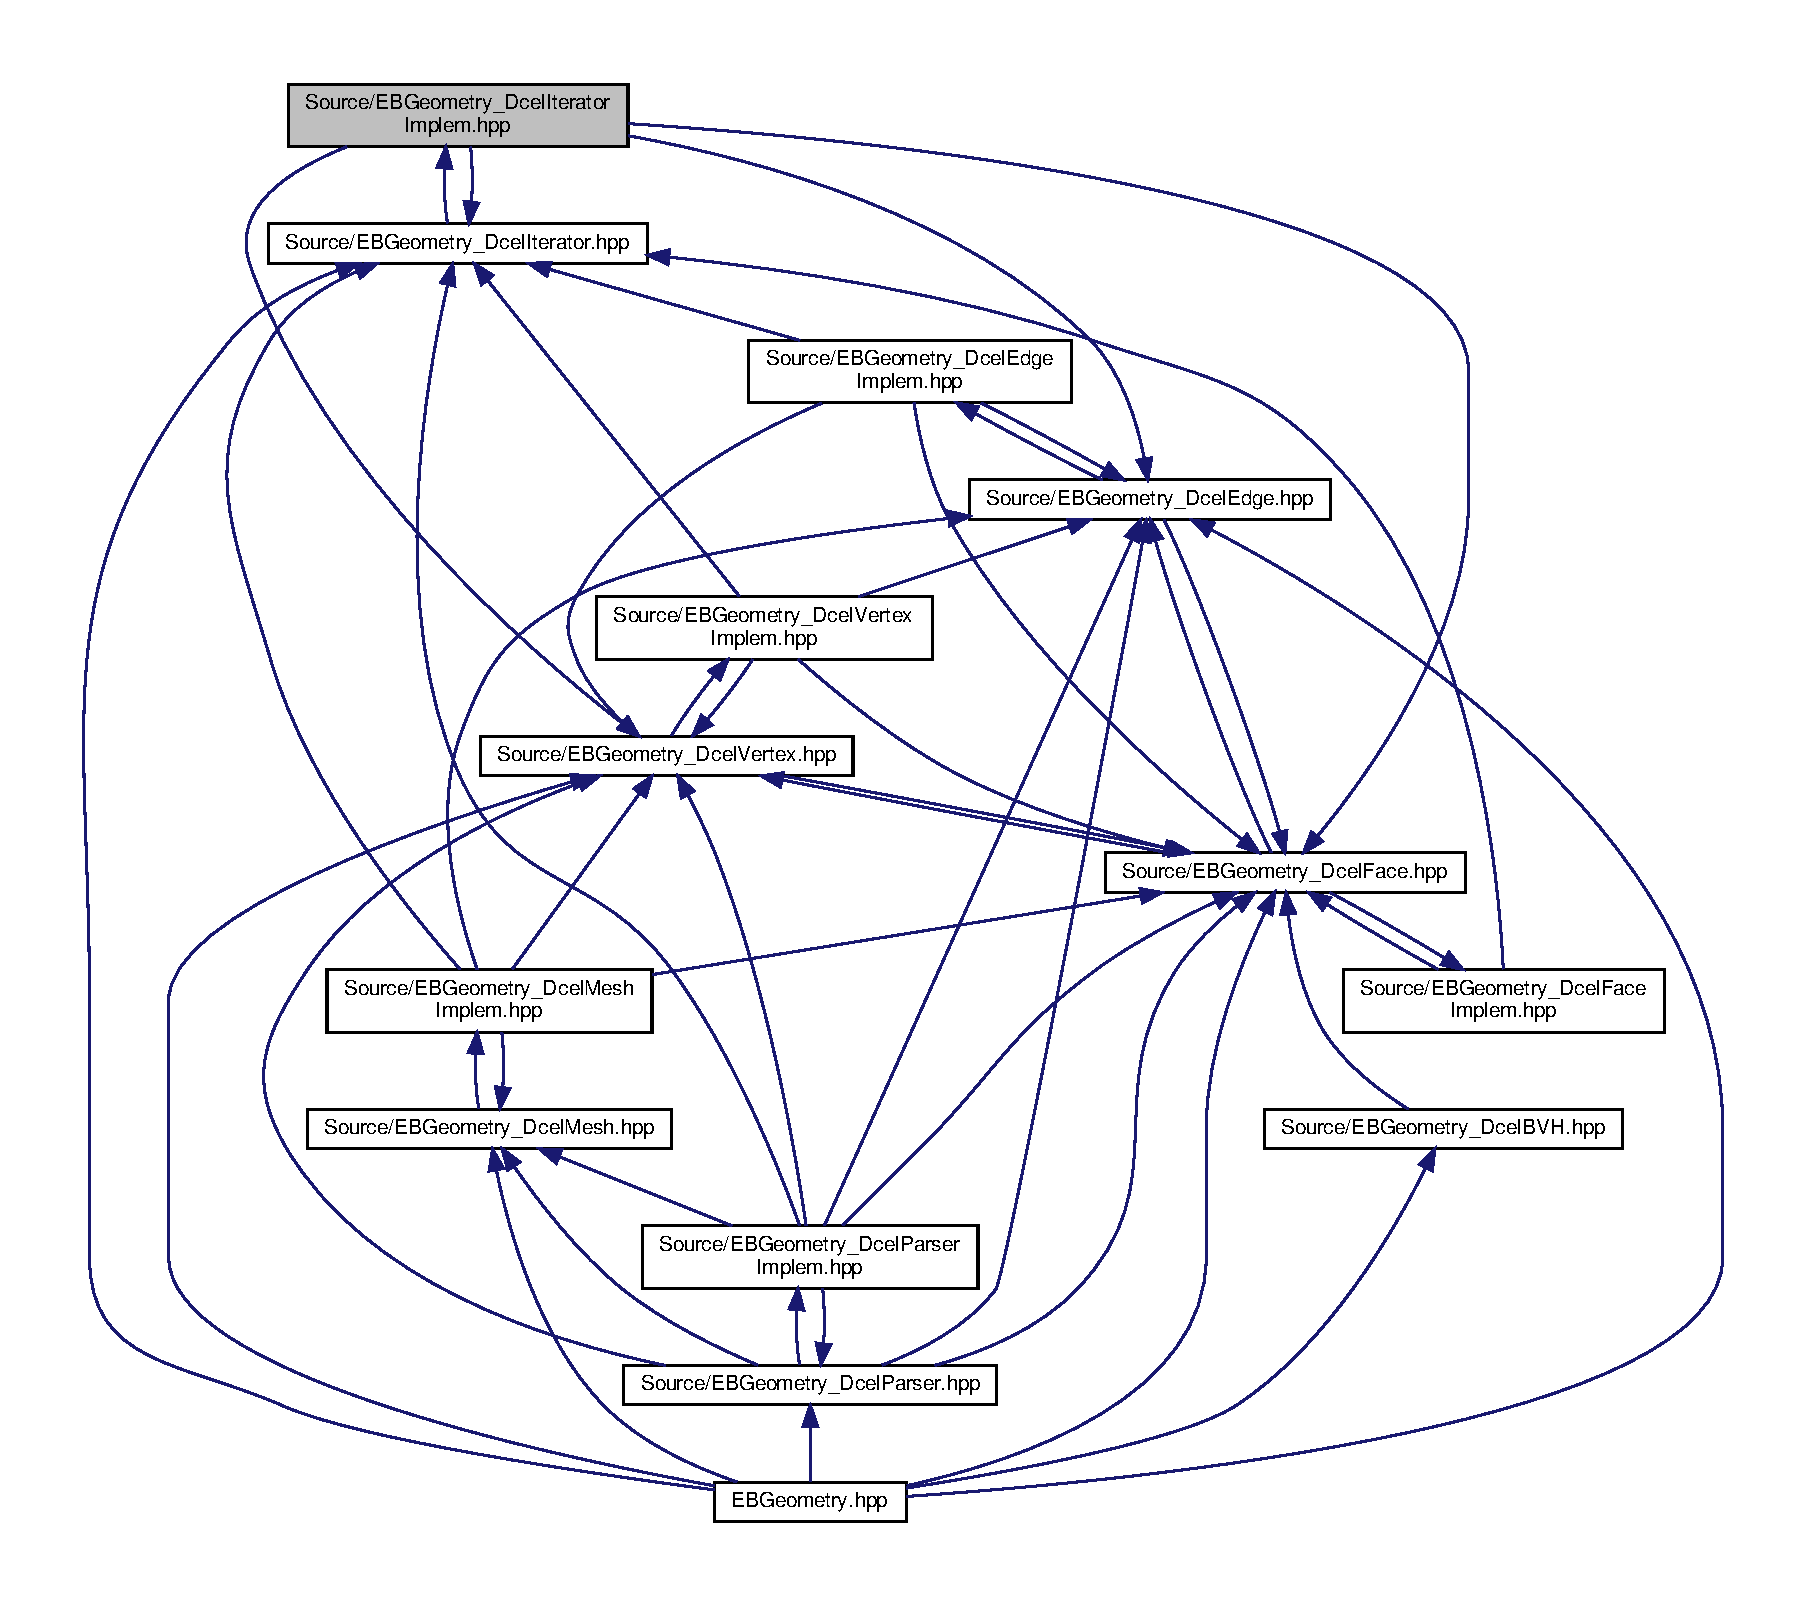
\includegraphics[width=350pt]{EBGeometry__DcelIteratorImplem_8hpp__dep__incl}
\end{center}
\end{figure}
\subsection*{Namespaces}
\begin{DoxyCompactItemize}
\item 
 \hyperlink{namespaceDcel}{Dcel}
\begin{DoxyCompactList}\small\item\em Namespace containing various double-\/connected edge list (D\+C\+EL) functionality. \end{DoxyCompactList}\end{DoxyCompactItemize}


\subsection{Detailed Description}
Implementation of \hyperlink{EBGeometry__DcelIterator_8hpp}{E\+B\+Geometry\+\_\+\+Dcel\+Iterator.\+hpp}. 

\begin{DoxyAuthor}{Author}
Robert Marskar 
\end{DoxyAuthor}

\hypertarget{EBGeometry__DcelMesh_8hpp}{}\section{Source/\+E\+B\+Geometry\+\_\+\+Dcel\+Mesh.hpp File Reference}
\label{EBGeometry__DcelMesh_8hpp}\index{Source/\+E\+B\+Geometry\+\_\+\+Dcel\+Mesh.\+hpp@{Source/\+E\+B\+Geometry\+\_\+\+Dcel\+Mesh.\+hpp}}


Declaration of a mesh class which stores a D\+C\+EL mesh (with signed distance functions)  


{\ttfamily \#include $<$vector$>$}\newline
{\ttfamily \#include $<$memory$>$}\newline
{\ttfamily \#include $<$functional$>$}\newline
{\ttfamily \#include $<$map$>$}\newline
{\ttfamily \#include \char`\"{}E\+B\+Geometry\+\_\+\+Dcel\+Polygon2\+D.\+hpp\char`\"{}}\newline
{\ttfamily \#include \char`\"{}E\+B\+Geometry\+\_\+\+Namespace\+Header.\+hpp\char`\"{}}\newline
{\ttfamily \#include \char`\"{}E\+B\+Geometry\+\_\+\+Namespace\+Footer.\+hpp\char`\"{}}\newline
{\ttfamily \#include \char`\"{}E\+B\+Geometry\+\_\+\+Dcel\+Mesh\+Implem.\+hpp\char`\"{}}\newline
Include dependency graph for E\+B\+Geometry\+\_\+\+Dcel\+Mesh.\+hpp\+:\nopagebreak
\begin{figure}[H]
\begin{center}
\leavevmode
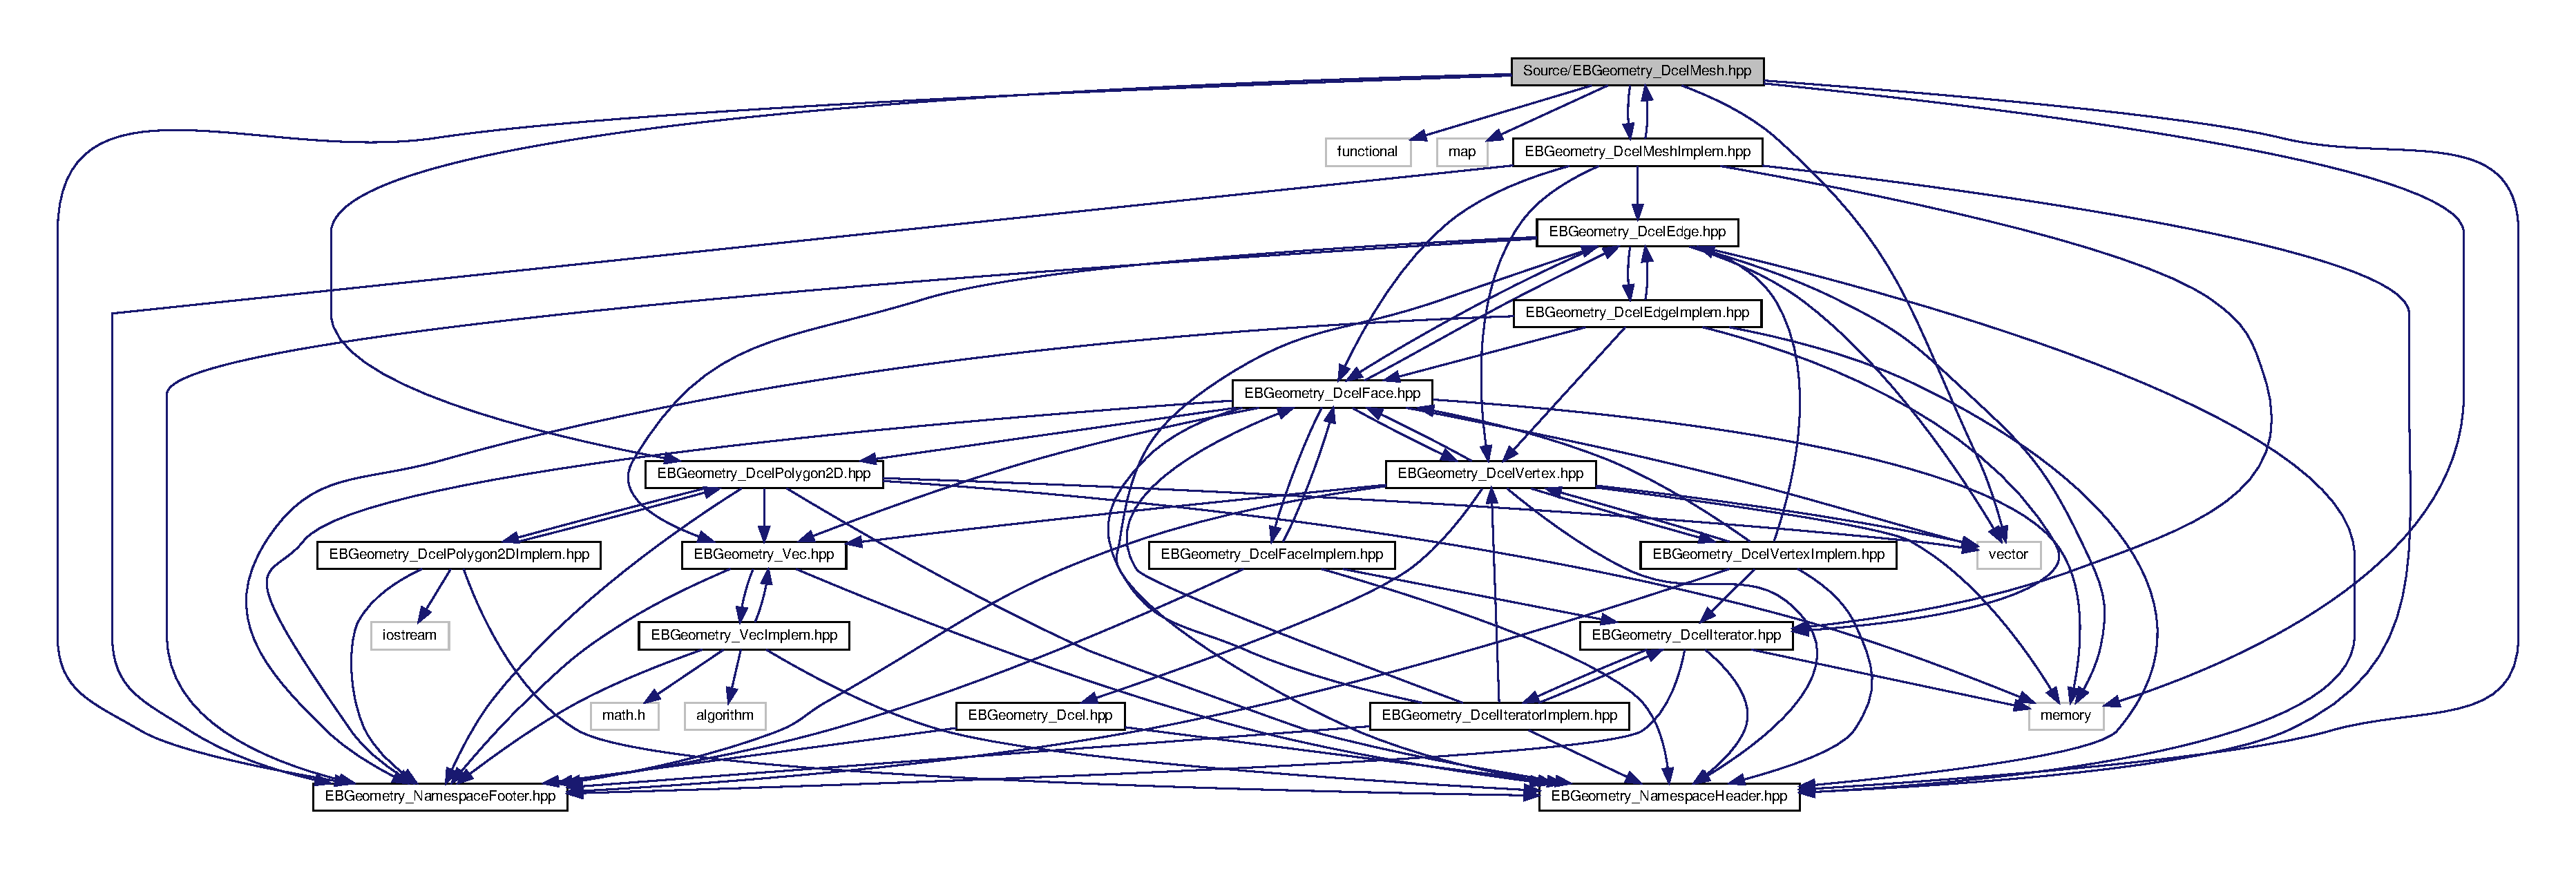
\includegraphics[width=350pt]{EBGeometry__DcelMesh_8hpp__incl}
\end{center}
\end{figure}
This graph shows which files directly or indirectly include this file\+:\nopagebreak
\begin{figure}[H]
\begin{center}
\leavevmode
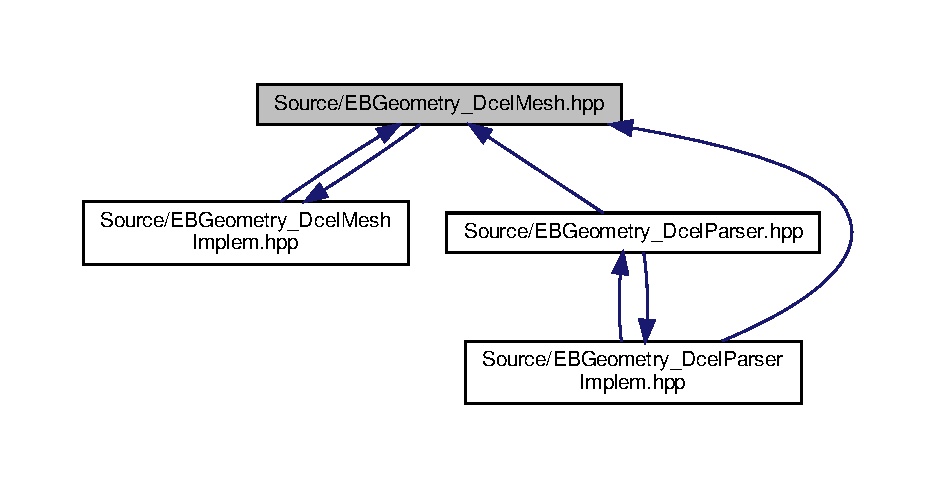
\includegraphics[width=350pt]{EBGeometry__DcelMesh_8hpp__dep__incl}
\end{center}
\end{figure}
\subsection*{Classes}
\begin{DoxyCompactItemize}
\item 
class \hyperlink{classDcel_1_1VertexT}{Dcel\+::\+Vertex\+T$<$ T $>$}
\begin{DoxyCompactList}\small\item\em Class which represents a vertex node in a double-\/edge connected list (D\+C\+EL). \end{DoxyCompactList}\item 
class \hyperlink{classDcel_1_1EdgeT}{Dcel\+::\+Edge\+T$<$ T $>$}
\begin{DoxyCompactList}\small\item\em Class which represents a half-\/edge in a double-\/edge connected list (D\+C\+EL). \end{DoxyCompactList}\item 
class \hyperlink{classDcel_1_1FaceT}{Dcel\+::\+Face\+T$<$ T $>$}
\begin{DoxyCompactList}\small\item\em Class which represents a polygon face in a double-\/edge connected list (D\+C\+EL). \end{DoxyCompactList}\item 
class \hyperlink{classDcel_1_1Polygon2D}{Dcel\+::\+Polygon2\+D$<$ T $>$}
\begin{DoxyCompactList}\small\item\em Class for embedding a D\+C\+EL polygon face into 2D. \end{DoxyCompactList}\item 
class \hyperlink{classDcel_1_1MeshT}{Dcel\+::\+Mesh\+T$<$ T $>$}
\begin{DoxyCompactList}\small\item\em Mesh class which stores a full D\+C\+EL mesh (with signed distance functions) \end{DoxyCompactList}\end{DoxyCompactItemize}
\subsection*{Namespaces}
\begin{DoxyCompactItemize}
\item 
 \hyperlink{namespaceDcel}{Dcel}
\begin{DoxyCompactList}\small\item\em Namespace containing various double-\/connected edge list (D\+C\+EL) functionality. \end{DoxyCompactList}\end{DoxyCompactItemize}


\subsection{Detailed Description}
Declaration of a mesh class which stores a D\+C\+EL mesh (with signed distance functions) 

\begin{DoxyAuthor}{Author}
Robert Marskar 
\end{DoxyAuthor}

\hypertarget{EBGeometry__DcelMeshImplem_8hpp}{}\section{Source/\+E\+B\+Geometry\+\_\+\+Dcel\+Mesh\+Implem.hpp File Reference}
\label{EBGeometry__DcelMeshImplem_8hpp}\index{Source/\+E\+B\+Geometry\+\_\+\+Dcel\+Mesh\+Implem.\+hpp@{Source/\+E\+B\+Geometry\+\_\+\+Dcel\+Mesh\+Implem.\+hpp}}


Implementation of \hyperlink{EBGeometry__DcelMesh_8hpp}{E\+B\+Geometry\+\_\+\+Dcel\+Mesh.\+hpp}.  


{\ttfamily \#include \char`\"{}E\+B\+Geometry\+\_\+\+Dcel\+Mesh.\+hpp\char`\"{}}\newline
{\ttfamily \#include \char`\"{}E\+B\+Geometry\+\_\+\+Dcel\+Iterator.\+hpp\char`\"{}}\newline
{\ttfamily \#include \char`\"{}E\+B\+Geometry\+\_\+\+Dcel\+Vertex.\+hpp\char`\"{}}\newline
{\ttfamily \#include \char`\"{}E\+B\+Geometry\+\_\+\+Dcel\+Edge.\+hpp\char`\"{}}\newline
{\ttfamily \#include \char`\"{}E\+B\+Geometry\+\_\+\+Dcel\+Face.\+hpp\char`\"{}}\newline
{\ttfamily \#include \char`\"{}E\+B\+Geometry\+\_\+\+Namespace\+Header.\+hpp\char`\"{}}\newline
{\ttfamily \#include \char`\"{}E\+B\+Geometry\+\_\+\+Namespace\+Footer.\+hpp\char`\"{}}\newline
Include dependency graph for E\+B\+Geometry\+\_\+\+Dcel\+Mesh\+Implem.\+hpp\+:\nopagebreak
\begin{figure}[H]
\begin{center}
\leavevmode
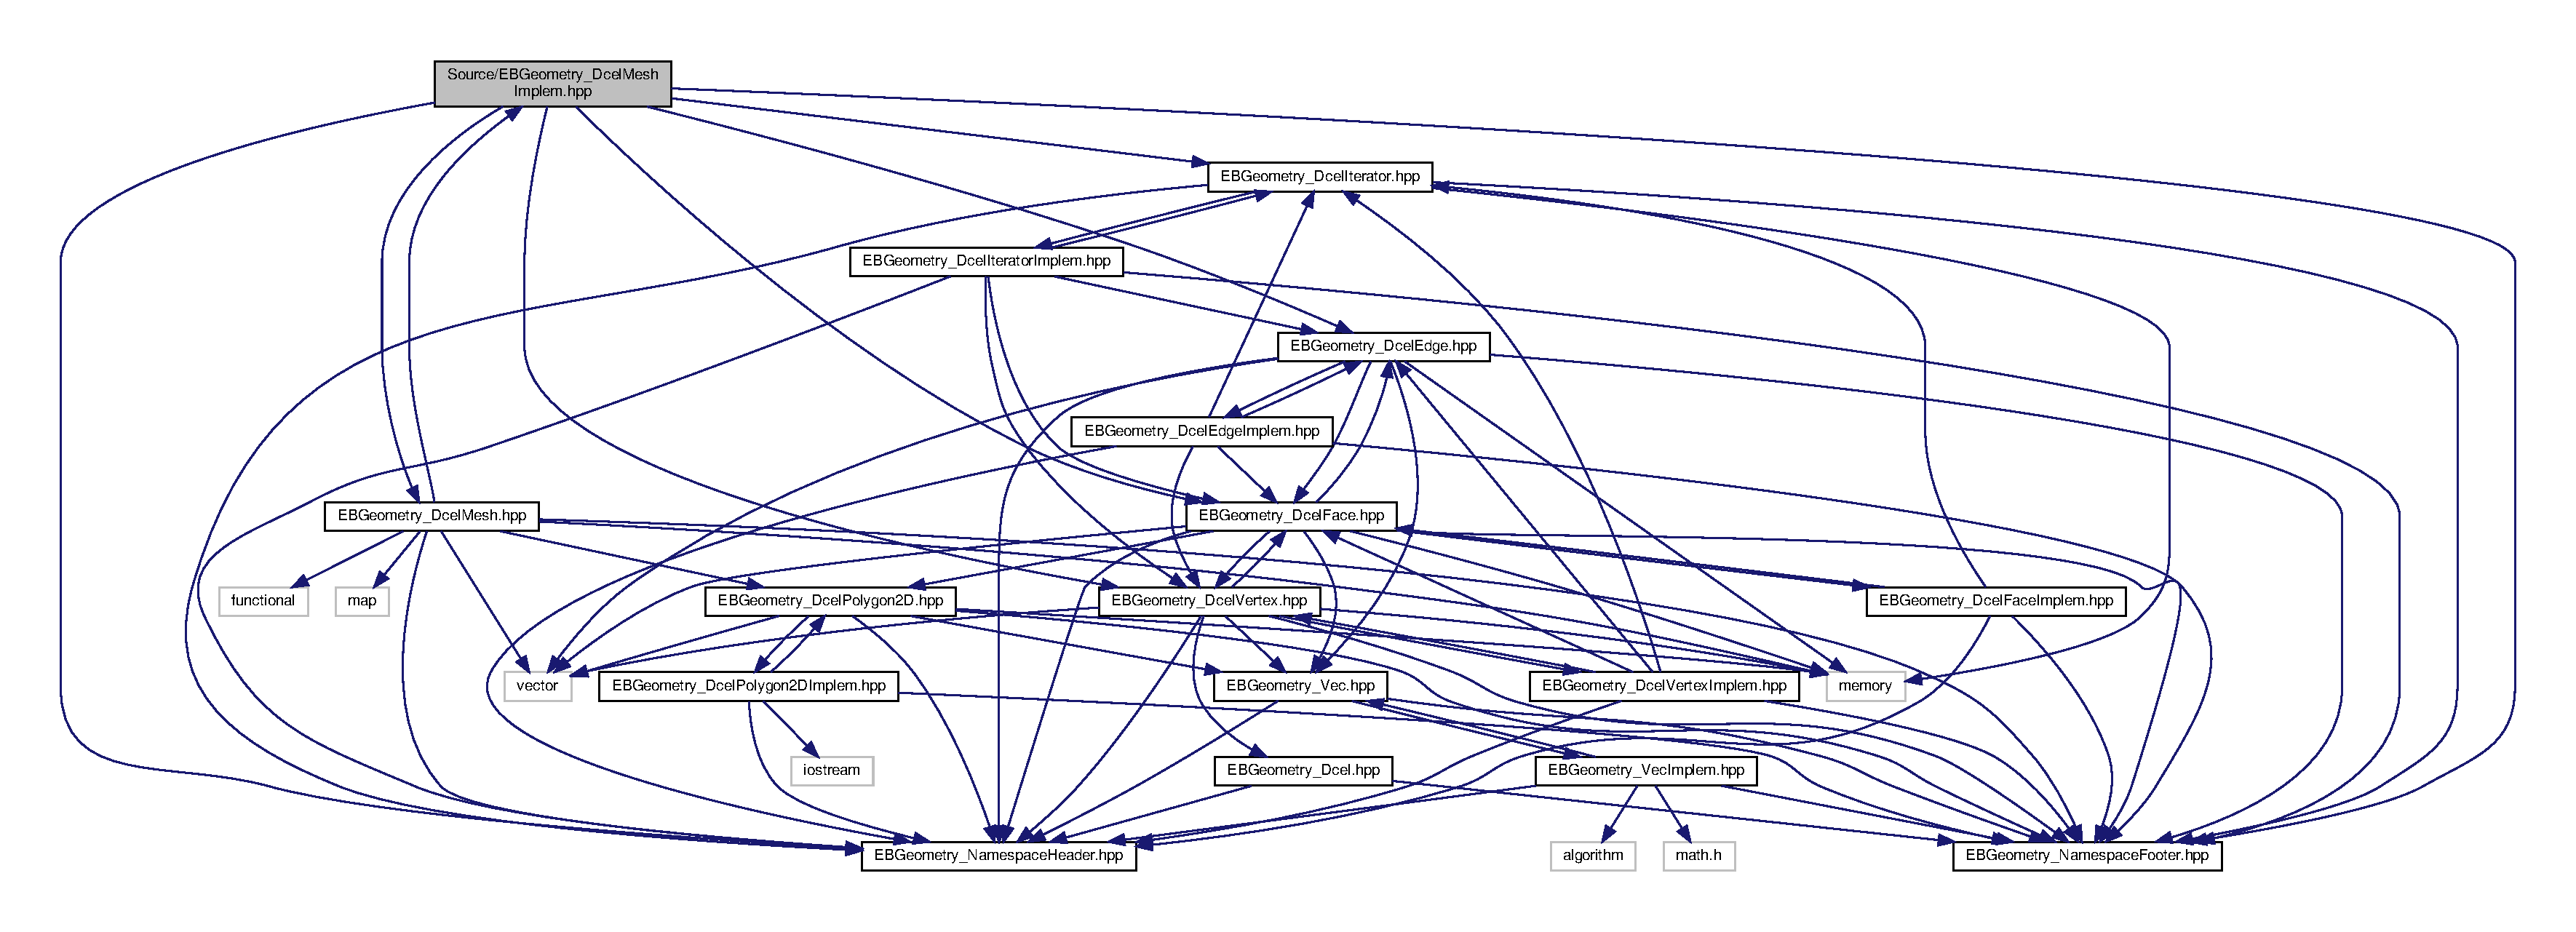
\includegraphics[width=350pt]{EBGeometry__DcelMeshImplem_8hpp__incl}
\end{center}
\end{figure}
This graph shows which files directly or indirectly include this file\+:\nopagebreak
\begin{figure}[H]
\begin{center}
\leavevmode
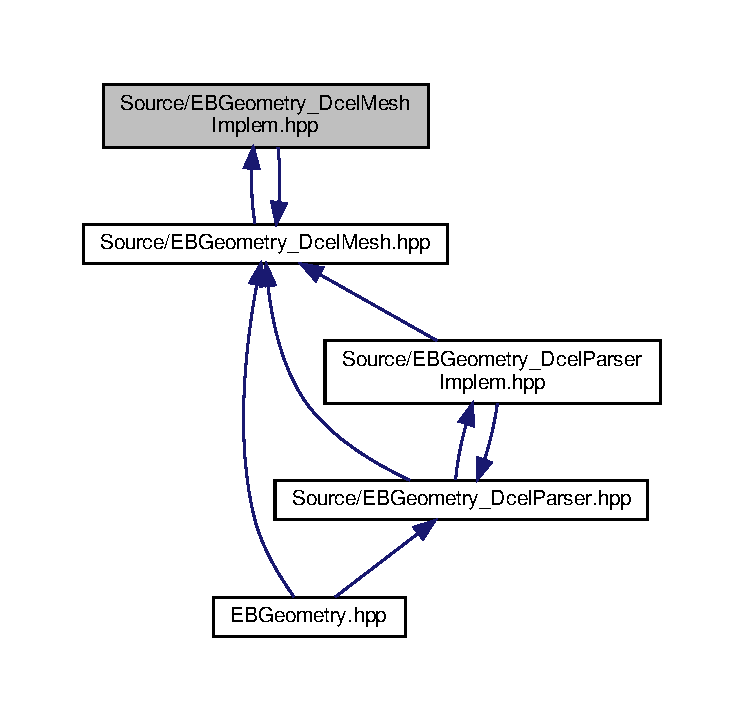
\includegraphics[width=350pt]{EBGeometry__DcelMeshImplem_8hpp__dep__incl}
\end{center}
\end{figure}
\subsection*{Namespaces}
\begin{DoxyCompactItemize}
\item 
 \hyperlink{namespaceDcel}{Dcel}
\begin{DoxyCompactList}\small\item\em Namespace containing various double-\/connected edge list (D\+C\+EL) functionality. \end{DoxyCompactList}\end{DoxyCompactItemize}


\subsection{Detailed Description}
Implementation of \hyperlink{EBGeometry__DcelMesh_8hpp}{E\+B\+Geometry\+\_\+\+Dcel\+Mesh.\+hpp}. 

\begin{DoxyAuthor}{Author}
Robert Marskar 
\end{DoxyAuthor}

\hypertarget{EBGeometry__DcelParser_8hpp}{}\section{Source/\+E\+B\+Geometry\+\_\+\+Dcel\+Parser.hpp File Reference}
\label{EBGeometry__DcelParser_8hpp}\index{Source/\+E\+B\+Geometry\+\_\+\+Dcel\+Parser.\+hpp@{Source/\+E\+B\+Geometry\+\_\+\+Dcel\+Parser.\+hpp}}


Declaration of utilities for passing data into D\+C\+EL structures.  


{\ttfamily \#include $<$vector$>$}\newline
{\ttfamily \#include $<$memory$>$}\newline
{\ttfamily \#include $<$map$>$}\newline
{\ttfamily \#include \char`\"{}E\+B\+Geometry\+\_\+\+Dcel\+Vertex.\+hpp\char`\"{}}\newline
{\ttfamily \#include \char`\"{}E\+B\+Geometry\+\_\+\+Dcel\+Edge.\+hpp\char`\"{}}\newline
{\ttfamily \#include \char`\"{}E\+B\+Geometry\+\_\+\+Dcel\+Face.\+hpp\char`\"{}}\newline
{\ttfamily \#include \char`\"{}E\+B\+Geometry\+\_\+\+Dcel\+Mesh.\+hpp\char`\"{}}\newline
{\ttfamily \#include \char`\"{}E\+B\+Geometry\+\_\+\+Namespace\+Header.\+hpp\char`\"{}}\newline
{\ttfamily \#include \char`\"{}E\+B\+Geometry\+\_\+\+Namespace\+Footer.\+hpp\char`\"{}}\newline
{\ttfamily \#include \char`\"{}E\+B\+Geometry\+\_\+\+Dcel\+Parser\+Implem.\+hpp\char`\"{}}\newline
Include dependency graph for E\+B\+Geometry\+\_\+\+Dcel\+Parser.\+hpp\+:\nopagebreak
\begin{figure}[H]
\begin{center}
\leavevmode
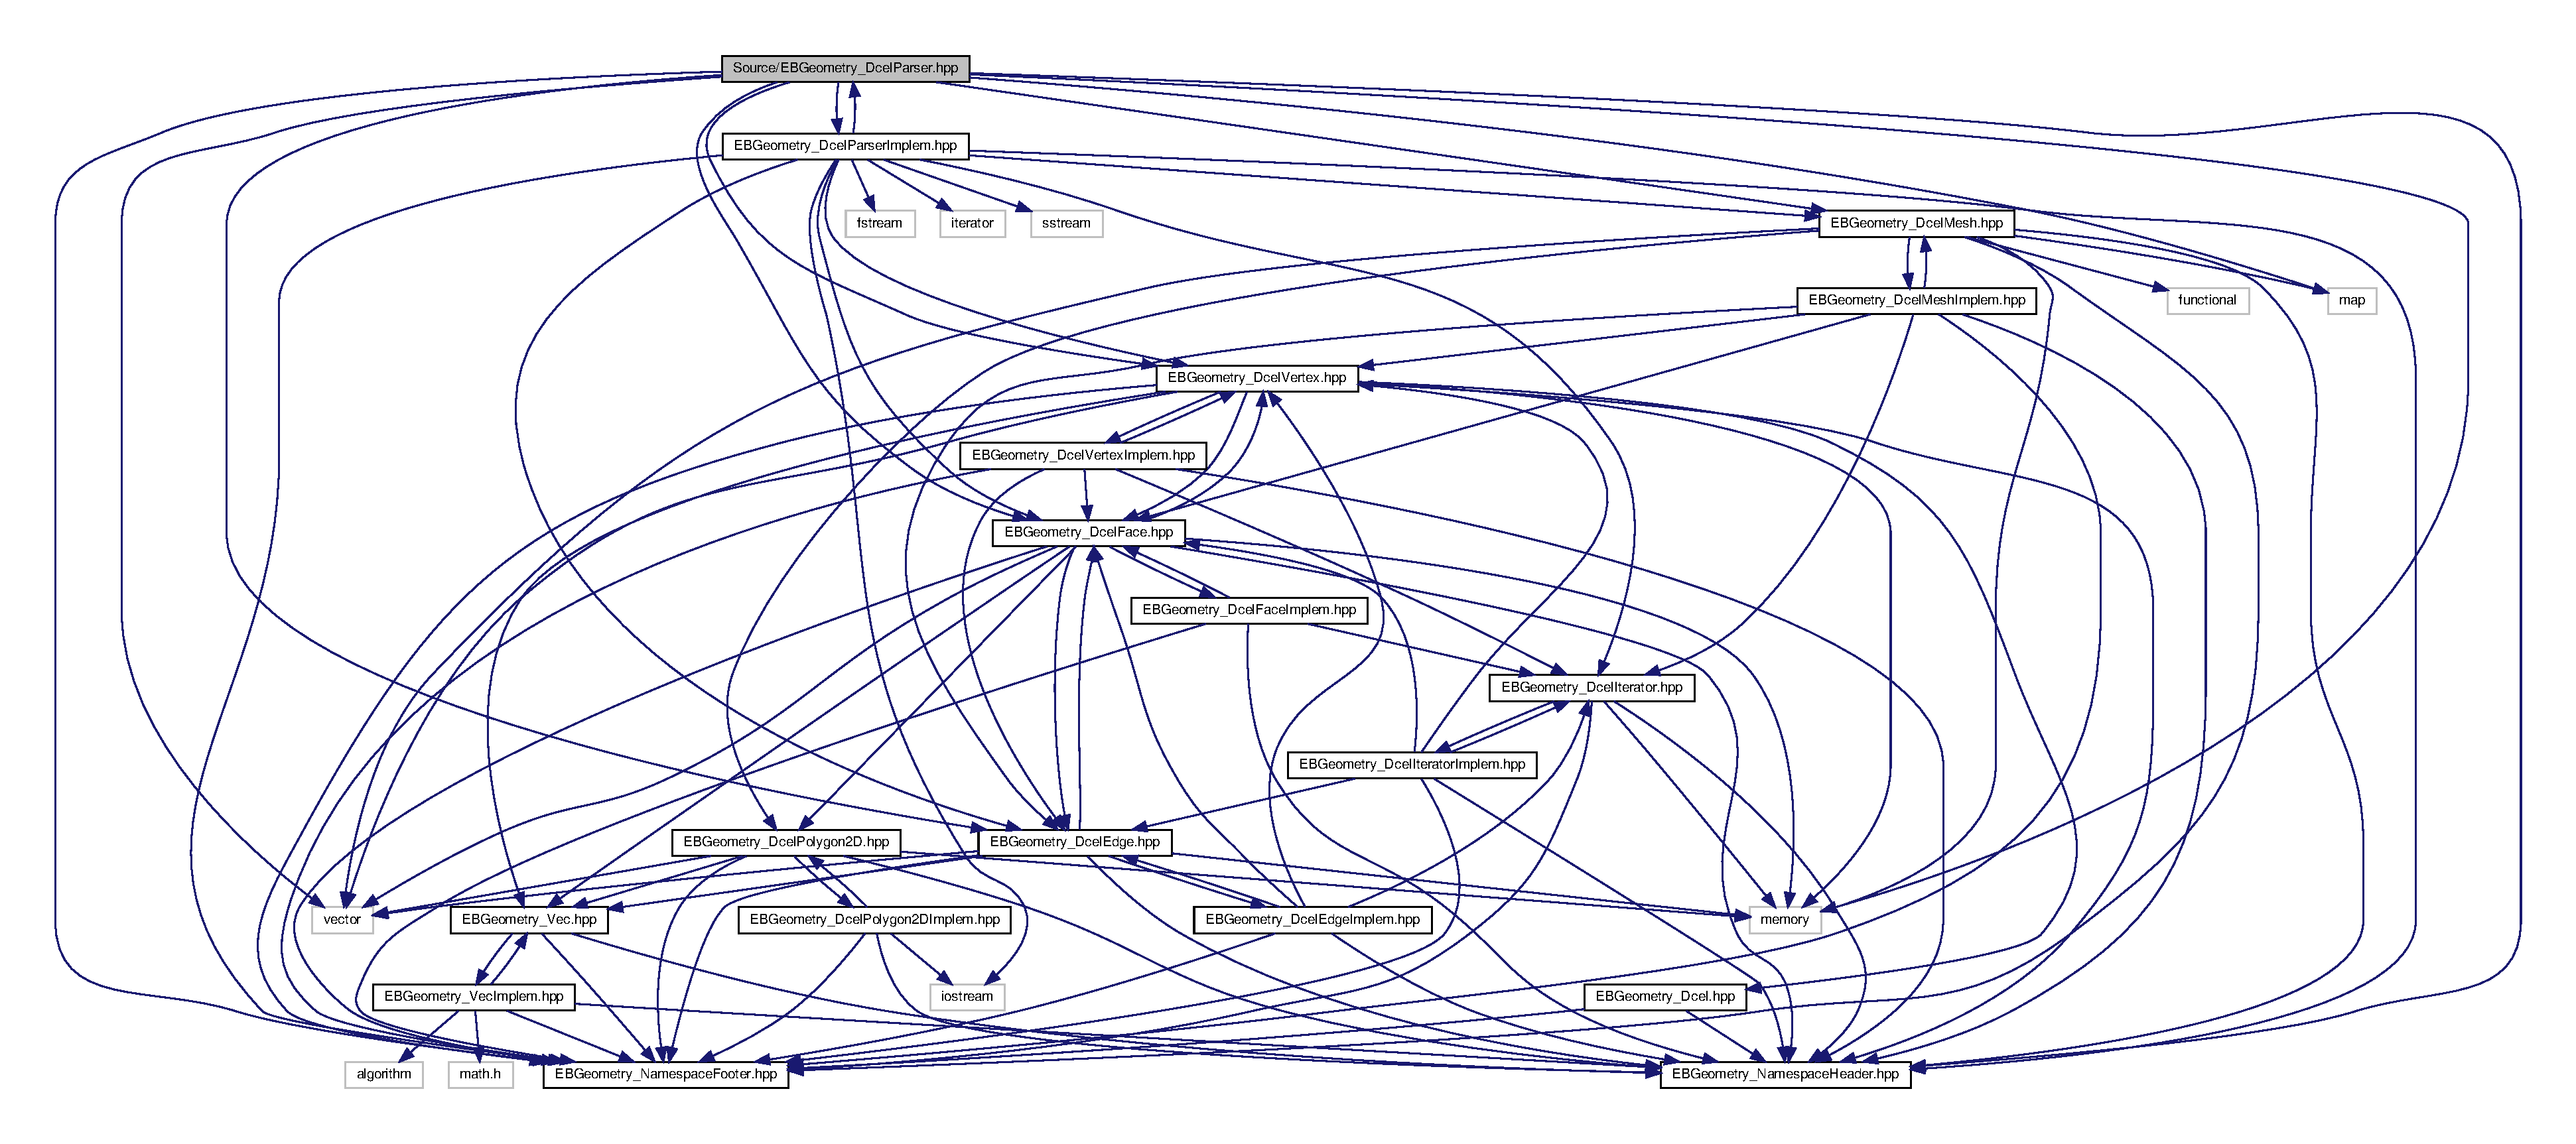
\includegraphics[width=350pt]{EBGeometry__DcelParser_8hpp__incl}
\end{center}
\end{figure}
This graph shows which files directly or indirectly include this file\+:\nopagebreak
\begin{figure}[H]
\begin{center}
\leavevmode
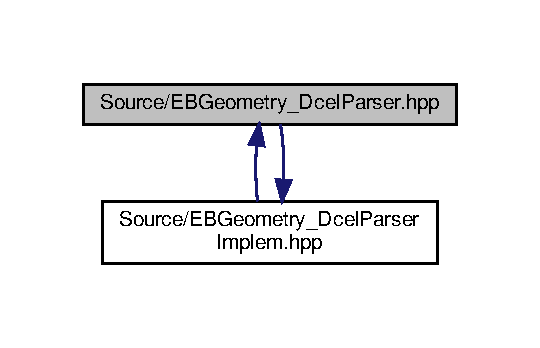
\includegraphics[width=350pt]{EBGeometry__DcelParser_8hpp__dep__incl}
\end{center}
\end{figure}
\subsection*{Classes}
\begin{DoxyCompactItemize}
\item 
class \hyperlink{classDcel_1_1Parser_1_1PLY}{Dcel\+::\+Parser\+::\+P\+L\+Y$<$ T $>$}
\begin{DoxyCompactList}\small\item\em Class for generation a Dcel\+::\+Mesh\+T$<$\+T$>$ from the Stanford \hyperlink{classDcel_1_1Parser_1_1PLY}{P\+LY} file format. \end{DoxyCompactList}\end{DoxyCompactItemize}
\subsection*{Namespaces}
\begin{DoxyCompactItemize}
\item 
 \hyperlink{namespaceDcel}{Dcel}
\begin{DoxyCompactList}\small\item\em Namespace containing various double-\/connected edge list (D\+C\+EL) functionality. \end{DoxyCompactList}\item 
 \hyperlink{namespaceDcel_1_1Parser}{Dcel\+::\+Parser}
\begin{DoxyCompactList}\small\item\em Namespace which encapsulates possible file parsers for building D\+C\+EL meshes. \end{DoxyCompactList}\end{DoxyCompactItemize}


\subsection{Detailed Description}
Declaration of utilities for passing data into D\+C\+EL structures. 

\begin{DoxyAuthor}{Author}
Robert Marskar 
\end{DoxyAuthor}

\hypertarget{EBGeometry__DcelParserImplem_8hpp}{}\doxysection{Source/\+E\+B\+Geometry\+\_\+\+Dcel\+Parser\+Implem.hpp File Reference}
\label{EBGeometry__DcelParserImplem_8hpp}\index{Source/EBGeometry\_DcelParserImplem.hpp@{Source/EBGeometry\_DcelParserImplem.hpp}}


Implementation of \mbox{\hyperlink{EBGeometry__DcelParser_8hpp}{E\+B\+Geometry\+\_\+\+Dcel\+Parser.\+hpp}}.  


{\ttfamily \#include $<$iostream$>$}\newline
{\ttfamily \#include $<$fstream$>$}\newline
{\ttfamily \#include $<$iterator$>$}\newline
{\ttfamily \#include $<$sstream$>$}\newline
{\ttfamily \#include \char`\"{}E\+B\+Geometry\+\_\+\+Dcel\+Parser.\+hpp\char`\"{}}\newline
{\ttfamily \#include \char`\"{}E\+B\+Geometry\+\_\+\+Dcel\+Vertex.\+hpp\char`\"{}}\newline
{\ttfamily \#include \char`\"{}E\+B\+Geometry\+\_\+\+Dcel\+Edge.\+hpp\char`\"{}}\newline
{\ttfamily \#include \char`\"{}E\+B\+Geometry\+\_\+\+Dcel\+Face.\+hpp\char`\"{}}\newline
{\ttfamily \#include \char`\"{}E\+B\+Geometry\+\_\+\+Dcel\+Mesh.\+hpp\char`\"{}}\newline
{\ttfamily \#include \char`\"{}E\+B\+Geometry\+\_\+\+Dcel\+Iterator.\+hpp\char`\"{}}\newline
{\ttfamily \#include \char`\"{}E\+B\+Geometry\+\_\+\+Namespace\+Header.\+hpp\char`\"{}}\newline
{\ttfamily \#include \char`\"{}E\+B\+Geometry\+\_\+\+Namespace\+Footer.\+hpp\char`\"{}}\newline
Include dependency graph for E\+B\+Geometry\+\_\+\+Dcel\+Parser\+Implem.\+hpp\+:
\nopagebreak
\begin{figure}[H]
\begin{center}
\leavevmode
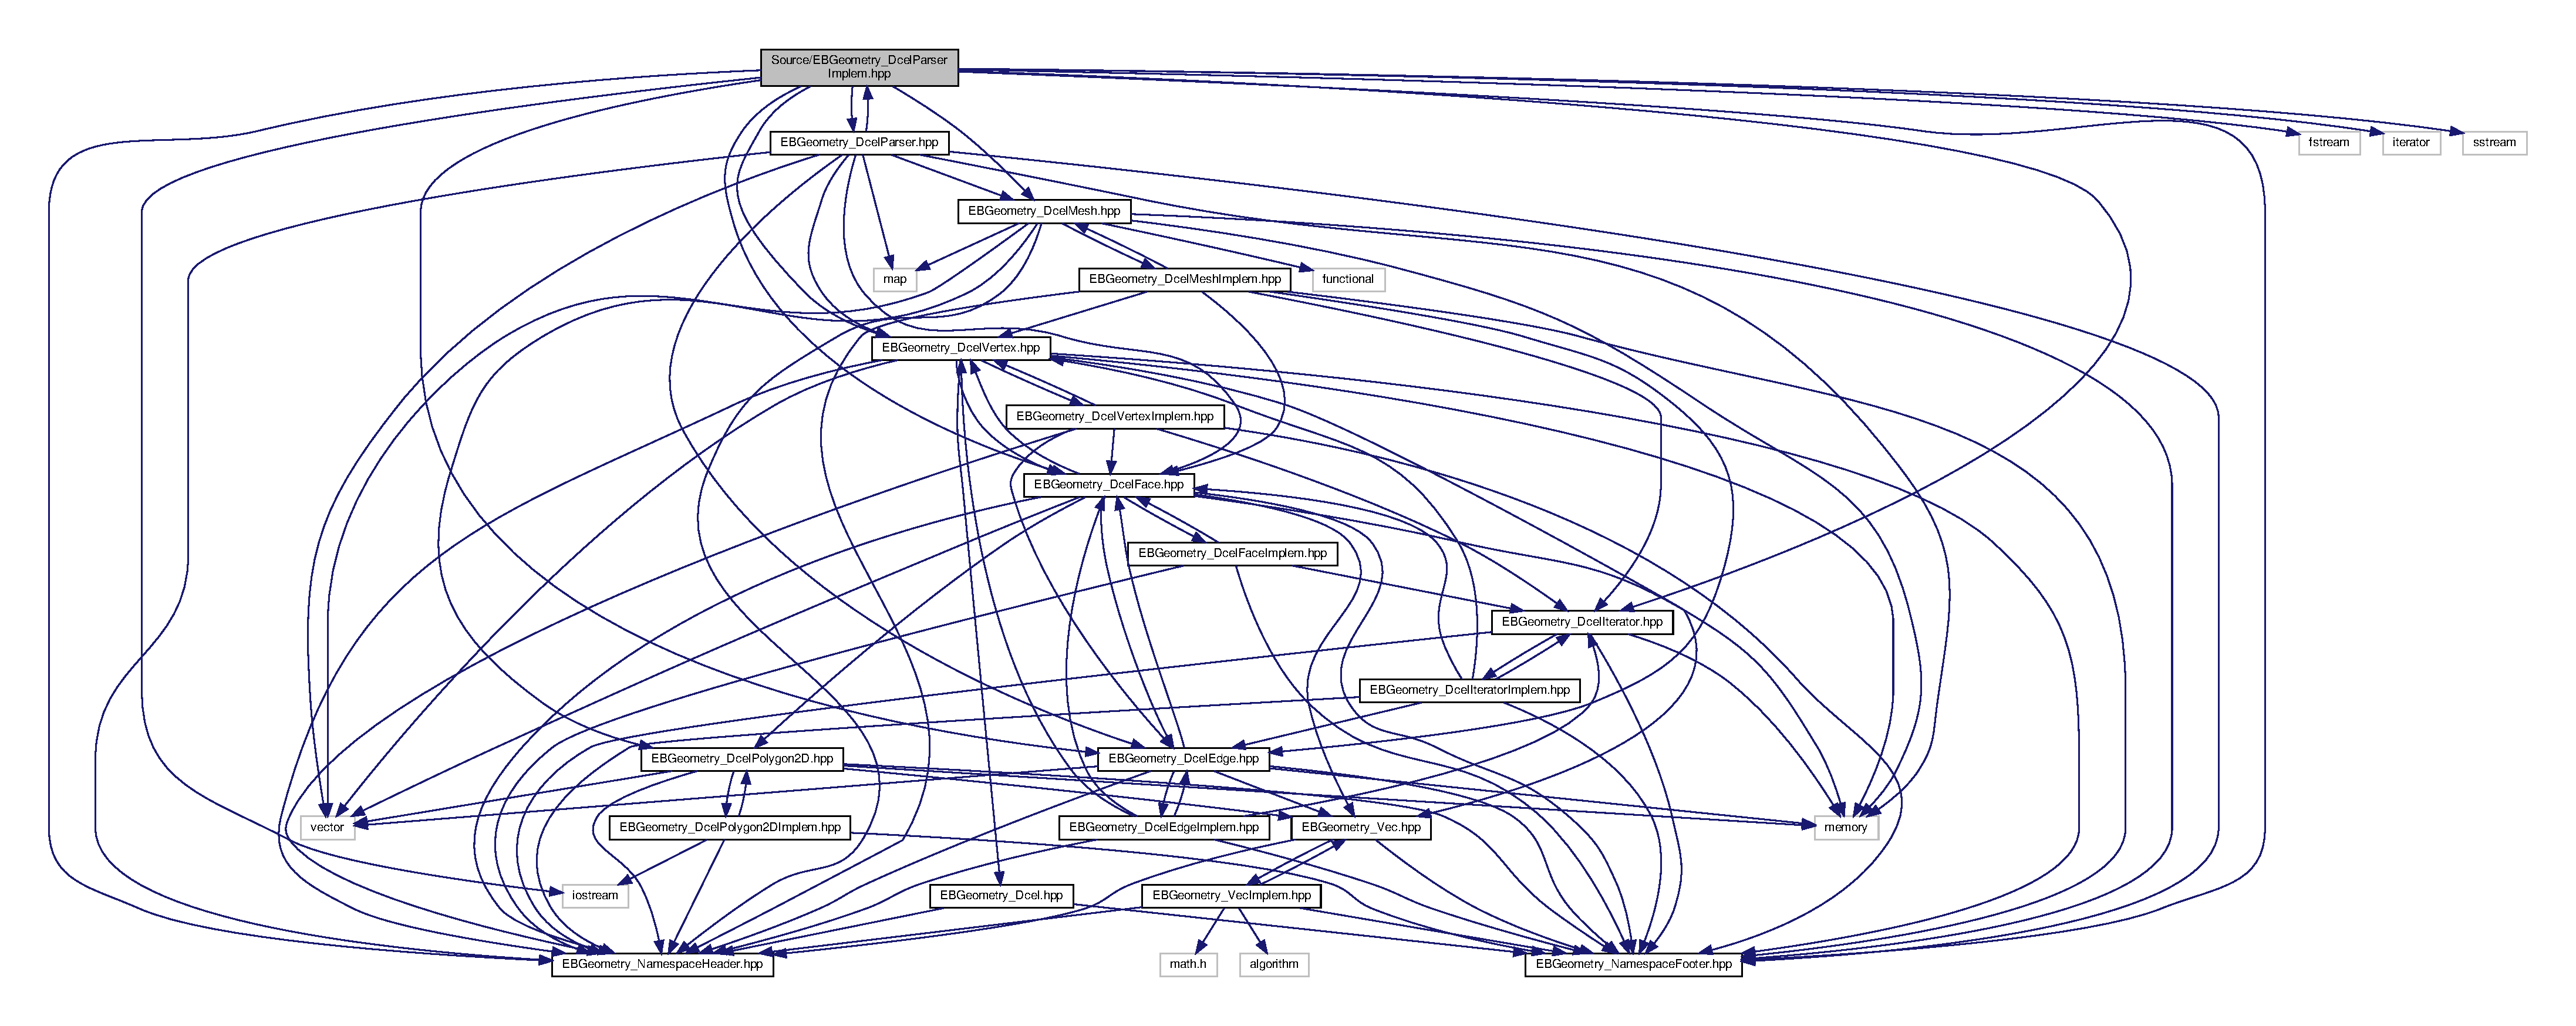
\includegraphics[width=350pt]{EBGeometry__DcelParserImplem_8hpp__incl}
\end{center}
\end{figure}
This graph shows which files directly or indirectly include this file\+:
\nopagebreak
\begin{figure}[H]
\begin{center}
\leavevmode
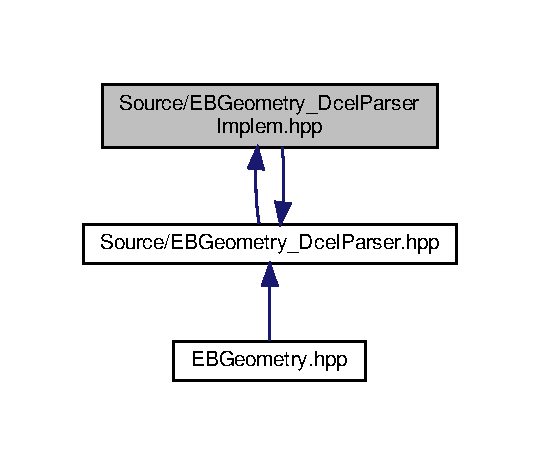
\includegraphics[width=271pt]{EBGeometry__DcelParserImplem_8hpp__dep__incl}
\end{center}
\end{figure}
\doxysubsection*{Namespaces}
\begin{DoxyCompactItemize}
\item 
 \mbox{\hyperlink{namespaceDcel}{Dcel}}
\begin{DoxyCompactList}\small\item\em Namespace containing various double-\/connected edge list (D\+C\+EL) functionality. \end{DoxyCompactList}\end{DoxyCompactItemize}


\doxysubsection{Detailed Description}
Implementation of \mbox{\hyperlink{EBGeometry__DcelParser_8hpp}{E\+B\+Geometry\+\_\+\+Dcel\+Parser.\+hpp}}. 

\begin{DoxyAuthor}{Author}
Robert Marskar 
\end{DoxyAuthor}

\hypertarget{EBGeometry__DcelPolygon2D_8hpp}{}\doxysection{Source/\+E\+B\+Geometry\+\_\+\+Dcel\+Polygon2D.hpp File Reference}
\label{EBGeometry__DcelPolygon2D_8hpp}\index{Source/EBGeometry\_DcelPolygon2D.hpp@{Source/EBGeometry\_DcelPolygon2D.hpp}}


Declaration of a two-\/dimensional polygon class for embedding 3D polygon faces.  


{\ttfamily \#include $<$memory$>$}\newline
{\ttfamily \#include $<$vector$>$}\newline
{\ttfamily \#include \char`\"{}E\+B\+Geometry\+\_\+\+Vec.\+hpp\char`\"{}}\newline
{\ttfamily \#include \char`\"{}E\+B\+Geometry\+\_\+\+Namespace\+Header.\+hpp\char`\"{}}\newline
{\ttfamily \#include \char`\"{}E\+B\+Geometry\+\_\+\+Namespace\+Footer.\+hpp\char`\"{}}\newline
{\ttfamily \#include \char`\"{}E\+B\+Geometry\+\_\+\+Dcel\+Polygon2\+D\+Implem.\+hpp\char`\"{}}\newline
Include dependency graph for E\+B\+Geometry\+\_\+\+Dcel\+Polygon2\+D.\+hpp\+:
\nopagebreak
\begin{figure}[H]
\begin{center}
\leavevmode
\includegraphics[width=350pt]{EBGeometry__DcelPolygon2D_8hpp__incl}
\end{center}
\end{figure}
This graph shows which files directly or indirectly include this file\+:
\nopagebreak
\begin{figure}[H]
\begin{center}
\leavevmode
\includegraphics[width=350pt]{EBGeometry__DcelPolygon2D_8hpp__dep__incl}
\end{center}
\end{figure}
\doxysubsection*{Classes}
\begin{DoxyCompactItemize}
\item 
class \mbox{\hyperlink{classDcel_1_1Polygon2D}{Dcel\+::\+Polygon2\+D$<$ T $>$}}
\begin{DoxyCompactList}\small\item\em Class for embedding a D\+C\+EL polygon face into 2D. \end{DoxyCompactList}\end{DoxyCompactItemize}
\doxysubsection*{Namespaces}
\begin{DoxyCompactItemize}
\item 
 \mbox{\hyperlink{namespaceDcel}{Dcel}}
\begin{DoxyCompactList}\small\item\em Namespace containing various double-\/connected edge list (D\+C\+EL) functionality. \end{DoxyCompactList}\end{DoxyCompactItemize}


\doxysubsection{Detailed Description}
Declaration of a two-\/dimensional polygon class for embedding 3D polygon faces. 

\begin{DoxyAuthor}{Author}
Robert Marskar 
\end{DoxyAuthor}

\hypertarget{EBGeometry__DcelPolygon2DImplem_8hpp}{}\doxysection{Source/\+E\+B\+Geometry\+\_\+\+Dcel\+Polygon2\+D\+Implem.hpp File Reference}
\label{EBGeometry__DcelPolygon2DImplem_8hpp}\index{Source/EBGeometry\_DcelPolygon2DImplem.hpp@{Source/EBGeometry\_DcelPolygon2DImplem.hpp}}


Implementation of Dcel\+Polygon.\+hpp.  


{\ttfamily \#include $<$iostream$>$}\newline
{\ttfamily \#include \char`\"{}E\+B\+Geometry\+\_\+\+Dcel\+Polygon2\+D.\+hpp\char`\"{}}\newline
{\ttfamily \#include \char`\"{}E\+B\+Geometry\+\_\+\+Namespace\+Header.\+hpp\char`\"{}}\newline
{\ttfamily \#include \char`\"{}E\+B\+Geometry\+\_\+\+Namespace\+Footer.\+hpp\char`\"{}}\newline
Include dependency graph for E\+B\+Geometry\+\_\+\+Dcel\+Polygon2\+D\+Implem.\+hpp\+:
\nopagebreak
\begin{figure}[H]
\begin{center}
\leavevmode
\includegraphics[width=350pt]{EBGeometry__DcelPolygon2DImplem_8hpp__incl}
\end{center}
\end{figure}
This graph shows which files directly or indirectly include this file\+:
\nopagebreak
\begin{figure}[H]
\begin{center}
\leavevmode
\includegraphics[width=350pt]{EBGeometry__DcelPolygon2DImplem_8hpp__dep__incl}
\end{center}
\end{figure}
\doxysubsection*{Namespaces}
\begin{DoxyCompactItemize}
\item 
 \mbox{\hyperlink{namespaceDcel}{Dcel}}
\begin{DoxyCompactList}\small\item\em Namespace containing various double-\/connected edge list (D\+C\+EL) functionality. \end{DoxyCompactList}\end{DoxyCompactItemize}


\doxysubsection{Detailed Description}
Implementation of Dcel\+Polygon.\+hpp. 

\begin{DoxyAuthor}{Author}
Robert Marskar 
\end{DoxyAuthor}

\hypertarget{EBGeometry__DcelVertex_8hpp}{}\doxysection{Source/\+E\+B\+Geometry\+\_\+\+Dcel\+Vertex.hpp File Reference}
\label{EBGeometry__DcelVertex_8hpp}\index{Source/EBGeometry\_DcelVertex.hpp@{Source/EBGeometry\_DcelVertex.hpp}}


Declaration of a vertex class for use in D\+C\+EL descriptions of polygon tesselations.  


{\ttfamily \#include $<$vector$>$}\newline
{\ttfamily \#include $<$memory$>$}\newline
{\ttfamily \#include \char`\"{}E\+B\+Geometry\+\_\+\+Vec.\+hpp\char`\"{}}\newline
{\ttfamily \#include \char`\"{}E\+B\+Geometry\+\_\+\+Dcel.\+hpp\char`\"{}}\newline
{\ttfamily \#include \char`\"{}E\+B\+Geometry\+\_\+\+Dcel\+Face.\+hpp\char`\"{}}\newline
{\ttfamily \#include \char`\"{}E\+B\+Geometry\+\_\+\+Namespace\+Header.\+hpp\char`\"{}}\newline
{\ttfamily \#include \char`\"{}E\+B\+Geometry\+\_\+\+Namespace\+Footer.\+hpp\char`\"{}}\newline
{\ttfamily \#include \char`\"{}E\+B\+Geometry\+\_\+\+Dcel\+Vertex\+Implem.\+hpp\char`\"{}}\newline
Include dependency graph for E\+B\+Geometry\+\_\+\+Dcel\+Vertex.\+hpp\+:
\nopagebreak
\begin{figure}[H]
\begin{center}
\leavevmode
\includegraphics[width=350pt]{EBGeometry__DcelVertex_8hpp__incl}
\end{center}
\end{figure}
This graph shows which files directly or indirectly include this file\+:
\nopagebreak
\begin{figure}[H]
\begin{center}
\leavevmode
\includegraphics[width=350pt]{EBGeometry__DcelVertex_8hpp__dep__incl}
\end{center}
\end{figure}
\doxysubsection*{Classes}
\begin{DoxyCompactItemize}
\item 
class \mbox{\hyperlink{classDcel_1_1VertexT}{Dcel\+::\+Vertex\+T$<$ T $>$}}
\begin{DoxyCompactList}\small\item\em Class which represents a vertex node in a double-\/edge connected list (D\+C\+EL). \end{DoxyCompactList}\item 
class \mbox{\hyperlink{classDcel_1_1EdgeT}{Dcel\+::\+Edge\+T$<$ T $>$}}
\begin{DoxyCompactList}\small\item\em Class which represents a half-\/edge in a double-\/edge connected list (D\+C\+EL). \end{DoxyCompactList}\item 
class \mbox{\hyperlink{classDcel_1_1FaceT}{Dcel\+::\+Face\+T$<$ T $>$}}
\begin{DoxyCompactList}\small\item\em Class which represents a polygon face in a double-\/edge connected list (D\+C\+EL). \end{DoxyCompactList}\item 
class \mbox{\hyperlink{classDcel_1_1EdgeIteratorT}{Dcel\+::\+Edge\+Iterator\+T$<$ T $>$}}
\begin{DoxyCompactList}\small\item\em Class which can iterate through edges and vertices around a D\+C\+EL polygon face. \end{DoxyCompactList}\item 
class \mbox{\hyperlink{classDcel_1_1VertexT}{Dcel\+::\+Vertex\+T$<$ T $>$}}
\begin{DoxyCompactList}\small\item\em Class which represents a vertex node in a double-\/edge connected list (D\+C\+EL). \end{DoxyCompactList}\end{DoxyCompactItemize}
\doxysubsection*{Namespaces}
\begin{DoxyCompactItemize}
\item 
 \mbox{\hyperlink{namespaceDcel}{Dcel}}
\begin{DoxyCompactList}\small\item\em Namespace containing various double-\/connected edge list (D\+C\+EL) functionality. \end{DoxyCompactList}\end{DoxyCompactItemize}


\doxysubsection{Detailed Description}
Declaration of a vertex class for use in D\+C\+EL descriptions of polygon tesselations. 

\begin{DoxyAuthor}{Author}
Robert Marskar 
\end{DoxyAuthor}

\hypertarget{EBGeometry__DcelVertexImplem_8hpp}{}\section{Source/\+E\+B\+Geometry\+\_\+\+Dcel\+Vertex\+Implem.hpp File Reference}
\label{EBGeometry__DcelVertexImplem_8hpp}\index{Source/\+E\+B\+Geometry\+\_\+\+Dcel\+Vertex\+Implem.\+hpp@{Source/\+E\+B\+Geometry\+\_\+\+Dcel\+Vertex\+Implem.\+hpp}}


Implementation of \hyperlink{EBGeometry__DcelVertex_8hpp}{E\+B\+Geometry\+\_\+\+Dcel\+Vertex.\+hpp}.  


{\ttfamily \#include \char`\"{}E\+B\+Geometry\+\_\+\+Dcel\+Vertex.\+hpp\char`\"{}}\newline
{\ttfamily \#include \char`\"{}E\+B\+Geometry\+\_\+\+Dcel\+Edge.\+hpp\char`\"{}}\newline
{\ttfamily \#include \char`\"{}E\+B\+Geometry\+\_\+\+Dcel\+Face.\+hpp\char`\"{}}\newline
{\ttfamily \#include \char`\"{}E\+B\+Geometry\+\_\+\+Dcel\+Iterator.\+hpp\char`\"{}}\newline
{\ttfamily \#include \char`\"{}E\+B\+Geometry\+\_\+\+Namespace\+Header.\+hpp\char`\"{}}\newline
{\ttfamily \#include \char`\"{}E\+B\+Geometry\+\_\+\+Namespace\+Footer.\+hpp\char`\"{}}\newline
Include dependency graph for E\+B\+Geometry\+\_\+\+Dcel\+Vertex\+Implem.\+hpp\+:\nopagebreak
\begin{figure}[H]
\begin{center}
\leavevmode
\includegraphics[width=350pt]{EBGeometry__DcelVertexImplem_8hpp__incl}
\end{center}
\end{figure}
This graph shows which files directly or indirectly include this file\+:\nopagebreak
\begin{figure}[H]
\begin{center}
\leavevmode
\includegraphics[width=350pt]{EBGeometry__DcelVertexImplem_8hpp__dep__incl}
\end{center}
\end{figure}
\subsection*{Namespaces}
\begin{DoxyCompactItemize}
\item 
 \hyperlink{namespaceDcel}{Dcel}
\begin{DoxyCompactList}\small\item\em Namespace containing various double-\/connected edge list (D\+C\+EL) functionality. \end{DoxyCompactList}\end{DoxyCompactItemize}


\subsection{Detailed Description}
Implementation of \hyperlink{EBGeometry__DcelVertex_8hpp}{E\+B\+Geometry\+\_\+\+Dcel\+Vertex.\+hpp}. 

\begin{DoxyAuthor}{Author}
Robert Marskar 
\end{DoxyAuthor}

\hypertarget{EBGeometry__NamespaceFooter_8hpp}{}\section{Source/\+E\+B\+Geometry\+\_\+\+Namespace\+Footer.hpp File Reference}
\label{EBGeometry__NamespaceFooter_8hpp}\index{Source/\+E\+B\+Geometry\+\_\+\+Namespace\+Footer.\+hpp@{Source/\+E\+B\+Geometry\+\_\+\+Namespace\+Footer.\+hpp}}


Name space footer.  


This graph shows which files directly or indirectly include this file\+:
\nopagebreak
\begin{figure}[H]
\begin{center}
\leavevmode
\includegraphics[width=350pt]{EBGeometry__NamespaceFooter_8hpp__dep__incl}
\end{center}
\end{figure}


\subsection{Detailed Description}
Name space footer. 

\begin{DoxyAuthor}{Author}
Robert Marskar 
\end{DoxyAuthor}

\hypertarget{EBGeometry__NamespaceHeader_8hpp}{}\section{Source/\+E\+B\+Geometry\+\_\+\+Namespace\+Header.hpp File Reference}
\label{EBGeometry__NamespaceHeader_8hpp}\index{Source/\+E\+B\+Geometry\+\_\+\+Namespace\+Header.\+hpp@{Source/\+E\+B\+Geometry\+\_\+\+Namespace\+Header.\+hpp}}


Name space header.  


This graph shows which files directly or indirectly include this file\+:\nopagebreak
\begin{figure}[H]
\begin{center}
\leavevmode
\includegraphics[width=350pt]{EBGeometry__NamespaceHeader_8hpp__dep__incl}
\end{center}
\end{figure}


\subsection{Detailed Description}
Name space header. 

\begin{DoxyAuthor}{Author}
Robert Marskar 
\end{DoxyAuthor}

\hypertarget{EBGeometry__SignedDistanceFunction_8hpp}{}\doxysection{Source/\+E\+B\+Geometry\+\_\+\+Signed\+Distance\+Function.hpp File Reference}
\label{EBGeometry__SignedDistanceFunction_8hpp}\index{Source/EBGeometry\_SignedDistanceFunction.hpp@{Source/EBGeometry\_SignedDistanceFunction.hpp}}


Abstract base class for representing a signed distance function.  


{\ttfamily \#include $<$memory$>$}\newline
{\ttfamily \#include $<$deque$>$}\newline
{\ttfamily \#include \char`\"{}E\+B\+Geometry\+\_\+\+Transform\+Ops.\+hpp\char`\"{}}\newline
{\ttfamily \#include \char`\"{}E\+B\+Geometry\+\_\+\+Namespace\+Header.\+hpp\char`\"{}}\newline
{\ttfamily \#include \char`\"{}E\+B\+Geometry\+\_\+\+Namespace\+Footer.\+hpp\char`\"{}}\newline
{\ttfamily \#include \char`\"{}E\+B\+Geometry\+\_\+\+Signed\+Distance\+Function\+Implem.\+hpp\char`\"{}}\newline
Include dependency graph for E\+B\+Geometry\+\_\+\+Signed\+Distance\+Function.\+hpp\+:
\nopagebreak
\begin{figure}[H]
\begin{center}
\leavevmode
\includegraphics[width=350pt]{EBGeometry__SignedDistanceFunction_8hpp__incl}
\end{center}
\end{figure}
This graph shows which files directly or indirectly include this file\+:
\nopagebreak
\begin{figure}[H]
\begin{center}
\leavevmode
\includegraphics[width=350pt]{EBGeometry__SignedDistanceFunction_8hpp__dep__incl}
\end{center}
\end{figure}
\doxysubsection*{Classes}
\begin{DoxyCompactItemize}
\item 
class \mbox{\hyperlink{classSignedDistanceFunction}{Signed\+Distance\+Function$<$ T $>$}}
\begin{DoxyCompactList}\small\item\em Abstract representation of a signed distance function. \end{DoxyCompactList}\end{DoxyCompactItemize}


\doxysubsection{Detailed Description}
Abstract base class for representing a signed distance function. 

\begin{DoxyAuthor}{Author}
Robert Marskar 
\end{DoxyAuthor}

\hypertarget{EBGeometry__SignedDistanceFunctionImplem_8hpp}{}\section{Source/\+E\+B\+Geometry\+\_\+\+Signed\+Distance\+Function\+Implem.hpp File Reference}
\label{EBGeometry__SignedDistanceFunctionImplem_8hpp}\index{Source/\+E\+B\+Geometry\+\_\+\+Signed\+Distance\+Function\+Implem.\+hpp@{Source/\+E\+B\+Geometry\+\_\+\+Signed\+Distance\+Function\+Implem.\+hpp}}


Implementation of \hyperlink{EBGeometry__SignedDistanceFunctionImplem_8hpp}{E\+B\+Geometry\+\_\+\+Signed\+Distance\+Function\+Implem.\+hpp}.  


{\ttfamily \#include \char`\"{}E\+B\+Geometry\+\_\+\+Signed\+Distance\+Function.\+hpp\char`\"{}}\newline
{\ttfamily \#include \char`\"{}E\+B\+Geometry\+\_\+\+Namespace\+Header.\+hpp\char`\"{}}\newline
{\ttfamily \#include \char`\"{}E\+B\+Geometry\+\_\+\+Namespace\+Footer.\+hpp\char`\"{}}\newline
Include dependency graph for E\+B\+Geometry\+\_\+\+Signed\+Distance\+Function\+Implem.\+hpp\+:\nopagebreak
\begin{figure}[H]
\begin{center}
\leavevmode
\includegraphics[width=350pt]{EBGeometry__SignedDistanceFunctionImplem_8hpp__incl}
\end{center}
\end{figure}
This graph shows which files directly or indirectly include this file\+:\nopagebreak
\begin{figure}[H]
\begin{center}
\leavevmode
\includegraphics[width=350pt]{EBGeometry__SignedDistanceFunctionImplem_8hpp__dep__incl}
\end{center}
\end{figure}


\subsection{Detailed Description}
Implementation of \hyperlink{EBGeometry__SignedDistanceFunctionImplem_8hpp}{E\+B\+Geometry\+\_\+\+Signed\+Distance\+Function\+Implem.\+hpp}. 

\begin{DoxyAuthor}{Author}
Robert Marskar 
\end{DoxyAuthor}

\hypertarget{EBGeometry__TransformOps_8hpp}{}\doxysection{/home/runner/work/\+E\+B\+Geometry/\+E\+B\+Geometry/\+Source/\+E\+B\+Geometry\+\_\+\+Transform\+Ops.hpp File Reference}
\label{EBGeometry__TransformOps_8hpp}\index{/home/runner/work/EBGeometry/EBGeometry/Source/EBGeometry\_TransformOps.hpp@{/home/runner/work/EBGeometry/EBGeometry/Source/EBGeometry\_TransformOps.hpp}}


Declaration of transformation operators for signed distance fields.  


{\ttfamily \#include \char`\"{}E\+B\+Geometry\+\_\+\+Vec.\+hpp\char`\"{}}\newline
{\ttfamily \#include \char`\"{}E\+B\+Geometry\+\_\+\+Namespace\+Header.\+hpp\char`\"{}}\newline
{\ttfamily \#include \char`\"{}E\+B\+Geometry\+\_\+\+Namespace\+Footer.\+hpp\char`\"{}}\newline
{\ttfamily \#include \char`\"{}E\+B\+Geometry\+\_\+\+Transform\+Ops\+Implem.\+hpp\char`\"{}}\newline
Include dependency graph for E\+B\+Geometry\+\_\+\+Transform\+Ops.\+hpp\+:
\nopagebreak
\begin{figure}[H]
\begin{center}
\leavevmode
\includegraphics[width=350pt]{EBGeometry__TransformOps_8hpp__incl}
\end{center}
\end{figure}
This graph shows which files directly or indirectly include this file\+:
\nopagebreak
\begin{figure}[H]
\begin{center}
\leavevmode
\includegraphics[width=350pt]{EBGeometry__TransformOps_8hpp__dep__incl}
\end{center}
\end{figure}
\doxysubsection*{Classes}
\begin{DoxyCompactItemize}
\item 
class \mbox{\hyperlink{classTransformOp}{Transform\+Op$<$ T $>$}}
\begin{DoxyCompactList}\small\item\em Base class for transformation operators. \end{DoxyCompactList}\item 
class \mbox{\hyperlink{classTranslateOp}{Translate\+Op$<$ T $>$}}
\begin{DoxyCompactList}\small\item\em Translation operator. Can translate an input point. \end{DoxyCompactList}\item 
class \mbox{\hyperlink{classRotateOp}{Rotate\+Op$<$ T $>$}}
\begin{DoxyCompactList}\small\item\em Rotation operator. Can scale an input point. \end{DoxyCompactList}\end{DoxyCompactItemize}


\doxysubsection{Detailed Description}
Declaration of transformation operators for signed distance fields. 

\begin{DoxyAuthor}{Author}
Robert Marskar 
\end{DoxyAuthor}

\hypertarget{EBGeometry__TransformOpsImplem_8hpp}{}\doxysection{/home/runner/work/\+E\+B\+Geometry/\+E\+B\+Geometry/\+Source/\+E\+B\+Geometry\+\_\+\+Transform\+Ops\+Implem.hpp File Reference}
\label{EBGeometry__TransformOpsImplem_8hpp}\index{/home/runner/work/EBGeometry/EBGeometry/Source/EBGeometry\_TransformOpsImplem.hpp@{/home/runner/work/EBGeometry/EBGeometry/Source/EBGeometry\_TransformOpsImplem.hpp}}


Implementation of \mbox{\hyperlink{EBGeometry__TransformOps_8hpp}{E\+B\+Geometry\+\_\+\+Transform\+Ops.\+hpp}}.  


{\ttfamily \#include \char`\"{}E\+B\+Geometry\+\_\+\+Transform\+Ops.\+hpp\char`\"{}}\newline
{\ttfamily \#include \char`\"{}E\+B\+Geometry\+\_\+\+Namespace\+Header.\+hpp\char`\"{}}\newline
{\ttfamily \#include \char`\"{}E\+B\+Geometry\+\_\+\+Namespace\+Footer.\+hpp\char`\"{}}\newline
Include dependency graph for E\+B\+Geometry\+\_\+\+Transform\+Ops\+Implem.\+hpp\+:
\nopagebreak
\begin{figure}[H]
\begin{center}
\leavevmode
\includegraphics[width=350pt]{EBGeometry__TransformOpsImplem_8hpp__incl}
\end{center}
\end{figure}
This graph shows which files directly or indirectly include this file\+:
\nopagebreak
\begin{figure}[H]
\begin{center}
\leavevmode
\includegraphics[width=350pt]{EBGeometry__TransformOpsImplem_8hpp__dep__incl}
\end{center}
\end{figure}


\doxysubsection{Detailed Description}
Implementation of \mbox{\hyperlink{EBGeometry__TransformOps_8hpp}{E\+B\+Geometry\+\_\+\+Transform\+Ops.\+hpp}}. 

\begin{DoxyAuthor}{Author}
Robert Marskar 
\end{DoxyAuthor}

\hypertarget{EBGeometry__Union_8hpp}{}\section{Source/\+E\+B\+Geometry\+\_\+\+Union.hpp File Reference}
\label{EBGeometry__Union_8hpp}\index{Source/\+E\+B\+Geometry\+\_\+\+Union.\+hpp@{Source/\+E\+B\+Geometry\+\_\+\+Union.\+hpp}}


Declaration of a union operator for creating multi-\/object scenes.  


{\ttfamily \#include $<$vector$>$}\newline
{\ttfamily \#include \char`\"{}E\+B\+Geometry\+\_\+\+Signed\+Distance\+Function.\+hpp\char`\"{}}\newline
{\ttfamily \#include \char`\"{}E\+B\+Geometry\+\_\+\+Namespace\+Header.\+hpp\char`\"{}}\newline
{\ttfamily \#include \char`\"{}E\+B\+Geometry\+\_\+\+Namespace\+Footer.\+hpp\char`\"{}}\newline
{\ttfamily \#include \char`\"{}E\+B\+Geometry\+\_\+\+Union\+Implem.\+hpp\char`\"{}}\newline
Include dependency graph for E\+B\+Geometry\+\_\+\+Union.\+hpp\+:\nopagebreak
\begin{figure}[H]
\begin{center}
\leavevmode
\includegraphics[width=350pt]{EBGeometry__Union_8hpp__incl}
\end{center}
\end{figure}
This graph shows which files directly or indirectly include this file\+:\nopagebreak
\begin{figure}[H]
\begin{center}
\leavevmode
\includegraphics[width=350pt]{EBGeometry__Union_8hpp__dep__incl}
\end{center}
\end{figure}
\subsection*{Classes}
\begin{DoxyCompactItemize}
\item 
class \hyperlink{classUnion}{Union$<$ T $>$}
\begin{DoxyCompactList}\small\item\em Distance function union. Computes the signed distance to the closest object of N non-\/overlapping objects. \end{DoxyCompactList}\end{DoxyCompactItemize}


\subsection{Detailed Description}
Declaration of a union operator for creating multi-\/object scenes. 

\begin{DoxyAuthor}{Author}
Robert Marskar 
\end{DoxyAuthor}

\hypertarget{EBGeometry__UnionBVH_8hpp}{}\section{Source/\+E\+B\+Geometry\+\_\+\+Union\+B\+VH.hpp File Reference}
\label{EBGeometry__UnionBVH_8hpp}\index{Source/\+E\+B\+Geometry\+\_\+\+Union\+B\+V\+H.\+hpp@{Source/\+E\+B\+Geometry\+\_\+\+Union\+B\+V\+H.\+hpp}}


Declaration of a union operator for creating multi-\/object scenes.  


{\ttfamily \#include $<$vector$>$}\newline
{\ttfamily \#include \char`\"{}E\+B\+Geometry\+\_\+\+Signed\+Distance\+Function.\+hpp\char`\"{}}\newline
{\ttfamily \#include \char`\"{}E\+B\+Geometry\+\_\+\+Namespace\+Header.\+hpp\char`\"{}}\newline
{\ttfamily \#include \char`\"{}E\+B\+Geometry\+\_\+\+Namespace\+Footer.\+hpp\char`\"{}}\newline
{\ttfamily \#include \char`\"{}E\+B\+Geometry\+\_\+\+Union\+B\+V\+H\+Implem.\+hpp\char`\"{}}\newline
Include dependency graph for E\+B\+Geometry\+\_\+\+Union\+B\+V\+H.\+hpp\+:\nopagebreak
\begin{figure}[H]
\begin{center}
\leavevmode
\includegraphics[width=350pt]{EBGeometry__UnionBVH_8hpp__incl}
\end{center}
\end{figure}
This graph shows which files directly or indirectly include this file\+:\nopagebreak
\begin{figure}[H]
\begin{center}
\leavevmode
\includegraphics[width=289pt]{EBGeometry__UnionBVH_8hpp__dep__incl}
\end{center}
\end{figure}
\subsection*{Classes}
\begin{DoxyCompactItemize}
\item 
class \hyperlink{classUnionBVH}{Union\+B\+V\+H$<$ T, B\+V, K $>$}
\begin{DoxyCompactList}\small\item\em Distance function union using B\+V\+Hs. Computes the signed distance to the closest object of N non-\/overlapping objects. \end{DoxyCompactList}\end{DoxyCompactItemize}


\subsection{Detailed Description}
Declaration of a union operator for creating multi-\/object scenes. 

\begin{DoxyAuthor}{Author}
Robert Marskar 
\end{DoxyAuthor}

\hypertarget{EBGeometry__UnionBVHImplem_8hpp}{}\doxysection{/home/runner/work/\+E\+B\+Geometry/\+E\+B\+Geometry/\+Source/\+E\+B\+Geometry\+\_\+\+Union\+B\+V\+H\+Implem.hpp File Reference}
\label{EBGeometry__UnionBVHImplem_8hpp}\index{/home/runner/work/EBGeometry/EBGeometry/Source/EBGeometry\_UnionBVHImplem.hpp@{/home/runner/work/EBGeometry/EBGeometry/Source/EBGeometry\_UnionBVHImplem.hpp}}


Implementation of \mbox{\hyperlink{EBGeometry__UnionBVH_8hpp}{E\+B\+Geometry\+\_\+\+Union\+B\+V\+H.\+hpp}}.  


{\ttfamily \#include \char`\"{}E\+B\+Geometry\+\_\+\+Union\+B\+V\+H.\+hpp\char`\"{}}\newline
{\ttfamily \#include \char`\"{}E\+B\+Geometry\+\_\+\+Namespace\+Header.\+hpp\char`\"{}}\newline
{\ttfamily \#include \char`\"{}E\+B\+Geometry\+\_\+\+Namespace\+Footer.\+hpp\char`\"{}}\newline
Include dependency graph for E\+B\+Geometry\+\_\+\+Union\+B\+V\+H\+Implem.\+hpp\+:
\nopagebreak
\begin{figure}[H]
\begin{center}
\leavevmode
\includegraphics[width=350pt]{EBGeometry__UnionBVHImplem_8hpp__incl}
\end{center}
\end{figure}
This graph shows which files directly or indirectly include this file\+:
\nopagebreak
\begin{figure}[H]
\begin{center}
\leavevmode
\includegraphics[width=262pt]{EBGeometry__UnionBVHImplem_8hpp__dep__incl}
\end{center}
\end{figure}


\doxysubsection{Detailed Description}
Implementation of \mbox{\hyperlink{EBGeometry__UnionBVH_8hpp}{E\+B\+Geometry\+\_\+\+Union\+B\+V\+H.\+hpp}}. 

\begin{DoxyAuthor}{Author}
Robert Marskar 
\end{DoxyAuthor}

\hypertarget{EBGeometry__UnionImplem_8hpp}{}\doxysection{/home/runner/work/\+E\+B\+Geometry/\+E\+B\+Geometry/\+Source/\+E\+B\+Geometry\+\_\+\+Union\+Implem.hpp File Reference}
\label{EBGeometry__UnionImplem_8hpp}\index{/home/runner/work/EBGeometry/EBGeometry/Source/EBGeometry\_UnionImplem.hpp@{/home/runner/work/EBGeometry/EBGeometry/Source/EBGeometry\_UnionImplem.hpp}}


Implementation of \mbox{\hyperlink{EBGeometry__Union_8hpp}{E\+B\+Geometry\+\_\+\+Union.\+hpp}}.  


{\ttfamily \#include \char`\"{}E\+B\+Geometry\+\_\+\+Union.\+hpp\char`\"{}}\newline
{\ttfamily \#include \char`\"{}E\+B\+Geometry\+\_\+\+Namespace\+Header.\+hpp\char`\"{}}\newline
{\ttfamily \#include \char`\"{}E\+B\+Geometry\+\_\+\+Namespace\+Footer.\+hpp\char`\"{}}\newline
Include dependency graph for E\+B\+Geometry\+\_\+\+Union\+Implem.\+hpp\+:
\nopagebreak
\begin{figure}[H]
\begin{center}
\leavevmode
\includegraphics[width=350pt]{EBGeometry__UnionImplem_8hpp__incl}
\end{center}
\end{figure}
This graph shows which files directly or indirectly include this file\+:
\nopagebreak
\begin{figure}[H]
\begin{center}
\leavevmode
\includegraphics[width=262pt]{EBGeometry__UnionImplem_8hpp__dep__incl}
\end{center}
\end{figure}


\doxysubsection{Detailed Description}
Implementation of \mbox{\hyperlink{EBGeometry__Union_8hpp}{E\+B\+Geometry\+\_\+\+Union.\+hpp}}. 

\begin{DoxyAuthor}{Author}
Robert Marskar 
\end{DoxyAuthor}

\hypertarget{EBGeometry__Vec_8hpp}{}\doxysection{Source/\+E\+B\+Geometry\+\_\+\+Vec.hpp File Reference}
\label{EBGeometry__Vec_8hpp}\index{Source/EBGeometry\_Vec.hpp@{Source/EBGeometry\_Vec.hpp}}


Declaration of 2D and 3D point/vector classes with templated precision. Used with \mbox{\hyperlink{namespaceDCEL}{D\+C\+EL}} tools.  


{\ttfamily \#include \char`\"{}E\+B\+Geometry\+\_\+\+Namespace\+Header.\+hpp\char`\"{}}\newline
{\ttfamily \#include \char`\"{}E\+B\+Geometry\+\_\+\+Namespace\+Footer.\+hpp\char`\"{}}\newline
{\ttfamily \#include \char`\"{}E\+B\+Geometry\+\_\+\+Vec\+Implem.\+hpp\char`\"{}}\newline
Include dependency graph for E\+B\+Geometry\+\_\+\+Vec.\+hpp\+:
\nopagebreak
\begin{figure}[H]
\begin{center}
\leavevmode
\includegraphics[width=350pt]{EBGeometry__Vec_8hpp__incl}
\end{center}
\end{figure}
This graph shows which files directly or indirectly include this file\+:
\nopagebreak
\begin{figure}[H]
\begin{center}
\leavevmode
\includegraphics[width=350pt]{EBGeometry__Vec_8hpp__dep__incl}
\end{center}
\end{figure}
\doxysubsection*{Classes}
\begin{DoxyCompactItemize}
\item 
class \mbox{\hyperlink{classVec2T}{Vec2\+T$<$ T $>$}}
\begin{DoxyCompactList}\small\item\em Two-\/dimensional vector class with arithmetic operators. \end{DoxyCompactList}\item 
class \mbox{\hyperlink{classVec3T}{Vec3\+T$<$ T $>$}}
\begin{DoxyCompactList}\small\item\em Three-\/dimensional vector class with arithmetic operators. \end{DoxyCompactList}\end{DoxyCompactItemize}
\doxysubsection*{Functions}
\begin{DoxyCompactItemize}
\item 
{\footnotesize template$<$class T $>$ }\\\mbox{\hyperlink{classVec2T}{Vec2T}}$<$ T $>$ \mbox{\hyperlink{EBGeometry__Vec_8hpp_a011c551978bb37db35ea3520fb23bd00}{operator$\ast$}} (const T \&s, const \mbox{\hyperlink{classVec2T}{Vec2T}}$<$ T $>$ \&a\+\_\+other) noexcept
\begin{DoxyCompactList}\small\item\em Multiplication operator in the form s$\ast$\+Vec2T. \end{DoxyCompactList}\item 
{\footnotesize template$<$class T $>$ }\\\mbox{\hyperlink{classVec2T}{Vec2T}}$<$ T $>$ \mbox{\hyperlink{EBGeometry__Vec_8hpp_a519f71e021376fe40b7d2f6e451fba02}{operator/}} (const T \&s, const \mbox{\hyperlink{classVec2T}{Vec2T}}$<$ T $>$ \&a\+\_\+other) noexcept
\begin{DoxyCompactList}\small\item\em Division operator in the form s$\ast$\+Vec2T. \end{DoxyCompactList}\item 
{\footnotesize template$<$class T $>$ }\\\mbox{\hyperlink{classVec3T}{Vec3T}}$<$ T $>$ \mbox{\hyperlink{EBGeometry__Vec_8hpp_affba8fd8ad3fc6110fbba33be5ad6187}{operator$\ast$}} (const T \&s, const \mbox{\hyperlink{classVec3T}{Vec3T}}$<$ T $>$ \&u) noexcept
\begin{DoxyCompactList}\small\item\em Multiplication operator. \end{DoxyCompactList}\item 
{\footnotesize template$<$class T $>$ }\\\mbox{\hyperlink{classVec3T}{Vec3T}}$<$ T $>$ \mbox{\hyperlink{EBGeometry__Vec_8hpp_aeeeedd62e251ff33f2e37286e391a0f8}{operator/}} (const T \&s, const \mbox{\hyperlink{classVec3T}{Vec3T}}$<$ T $>$ \&u) noexcept
\begin{DoxyCompactList}\small\item\em Division operator. \end{DoxyCompactList}\item 
{\footnotesize template$<$class T $>$ }\\\mbox{\hyperlink{classVec3T}{Vec3T}}$<$ T $>$ \mbox{\hyperlink{EBGeometry__Vec_8hpp_a291f01622695ab94c0092c3af0a1f3ca}{min}} (const \mbox{\hyperlink{classVec3T}{Vec3T}}$<$ T $>$ \&u, const \mbox{\hyperlink{classVec3T}{Vec3T}}$<$ T $>$ \&v) noexcept
\begin{DoxyCompactList}\small\item\em Minimum function. Returns new vector with component-\/wise minimums. \end{DoxyCompactList}\item 
{\footnotesize template$<$class T $>$ }\\\mbox{\hyperlink{classVec3T}{Vec3T}}$<$ T $>$ \mbox{\hyperlink{EBGeometry__Vec_8hpp_a71f0bc32c9be501cf01a1b6c715dc0a9}{max}} (const \mbox{\hyperlink{classVec3T}{Vec3T}}$<$ T $>$ \&u, const \mbox{\hyperlink{classVec3T}{Vec3T}}$<$ T $>$ \&v) noexcept
\begin{DoxyCompactList}\small\item\em Maximum function. Returns new vector with component-\/wise minimums. \end{DoxyCompactList}\item 
{\footnotesize template$<$class T $>$ }\\T \mbox{\hyperlink{EBGeometry__Vec_8hpp_a3f91a5c6f34c32789ab4760665810a9a}{dot}} (const \mbox{\hyperlink{classVec3T}{Vec3T}}$<$ T $>$ \&u, const \mbox{\hyperlink{classVec3T}{Vec3T}}$<$ T $>$ \&v) noexcept
\begin{DoxyCompactList}\small\item\em Dot product function. \end{DoxyCompactList}\item 
{\footnotesize template$<$class T $>$ }\\T \mbox{\hyperlink{EBGeometry__Vec_8hpp_aa7f7e15df344c873d1a27b30f77d0831}{length}} (const \mbox{\hyperlink{classVec3T}{Vec3T}}$<$ T $>$ \&v) noexcept
\begin{DoxyCompactList}\small\item\em Length function. \end{DoxyCompactList}\item 
{\footnotesize template$<$class T $>$ }\\\mbox{\hyperlink{classVec2T}{Vec2T}}$<$ T $>$ \mbox{\hyperlink{EBGeometry__Vec_8hpp_af9ce43058d66582ec3736b13a7ca5dc2}{min}} (const \mbox{\hyperlink{classVec2T}{Vec2T}}$<$ T $>$ \&u, const \mbox{\hyperlink{classVec2T}{Vec2T}}$<$ T $>$ \&v) noexcept
\begin{DoxyCompactList}\small\item\em Minimum function. Returns new vector with component-\/wise minimums. \end{DoxyCompactList}\item 
{\footnotesize template$<$class T $>$ }\\\mbox{\hyperlink{classVec2T}{Vec2T}}$<$ T $>$ \mbox{\hyperlink{EBGeometry__Vec_8hpp_a49e4d83079ba2af66014b14d2cf9fffd}{max}} (const \mbox{\hyperlink{classVec2T}{Vec2T}}$<$ T $>$ \&u, const \mbox{\hyperlink{classVec2T}{Vec2T}}$<$ T $>$ \&v) noexcept
\begin{DoxyCompactList}\small\item\em Maximum function. Returns new vector with component-\/wise minimums. \end{DoxyCompactList}\item 
{\footnotesize template$<$class T $>$ }\\T \mbox{\hyperlink{EBGeometry__Vec_8hpp_adfdac8ac7b17d6c165b7296d8f1b8780}{dot}} (const \mbox{\hyperlink{classVec2T}{Vec2T}}$<$ T $>$ \&u, const \mbox{\hyperlink{classVec2T}{Vec2T}}$<$ T $>$ \&v) noexcept
\begin{DoxyCompactList}\small\item\em Dot product function. \end{DoxyCompactList}\item 
{\footnotesize template$<$class T $>$ }\\T \mbox{\hyperlink{EBGeometry__Vec_8hpp_ac7cf88fcdf43f2f197b741a126274cab}{length}} (const \mbox{\hyperlink{classVec2T}{Vec2T}}$<$ T $>$ \&v) noexcept
\begin{DoxyCompactList}\small\item\em Length function. \end{DoxyCompactList}\end{DoxyCompactItemize}


\doxysubsection{Detailed Description}
Declaration of 2D and 3D point/vector classes with templated precision. Used with \mbox{\hyperlink{namespaceDCEL}{D\+C\+EL}} tools. 

\begin{DoxyAuthor}{Author}
Robert Marskar 
\end{DoxyAuthor}


\doxysubsection{Function Documentation}
\mbox{\Hypertarget{EBGeometry__Vec_8hpp_adfdac8ac7b17d6c165b7296d8f1b8780}\label{EBGeometry__Vec_8hpp_adfdac8ac7b17d6c165b7296d8f1b8780}} 
\index{EBGeometry\_Vec.hpp@{EBGeometry\_Vec.hpp}!dot@{dot}}
\index{dot@{dot}!EBGeometry\_Vec.hpp@{EBGeometry\_Vec.hpp}}
\doxysubsubsection{\texorpdfstring{dot()}{dot()}\hspace{0.1cm}{\footnotesize\ttfamily [1/2]}}
{\footnotesize\ttfamily template$<$class T $>$ \\
T dot (\begin{DoxyParamCaption}\item[{const \mbox{\hyperlink{classVec2T}{Vec2T}}$<$ T $>$ \&}]{u,  }\item[{const \mbox{\hyperlink{classVec2T}{Vec2T}}$<$ T $>$ \&}]{v }\end{DoxyParamCaption})\hspace{0.3cm}{\ttfamily [inline]}, {\ttfamily [noexcept]}}



Dot product function. 


\begin{DoxyParams}[1]{Parameters}
\mbox{\texttt{ in}}  & {\em u} & Vector \\
\hline
\mbox{\texttt{ in}}  & {\em v} & Other vector \\
\hline
\end{DoxyParams}
\mbox{\Hypertarget{EBGeometry__Vec_8hpp_a3f91a5c6f34c32789ab4760665810a9a}\label{EBGeometry__Vec_8hpp_a3f91a5c6f34c32789ab4760665810a9a}} 
\index{EBGeometry\_Vec.hpp@{EBGeometry\_Vec.hpp}!dot@{dot}}
\index{dot@{dot}!EBGeometry\_Vec.hpp@{EBGeometry\_Vec.hpp}}
\doxysubsubsection{\texorpdfstring{dot()}{dot()}\hspace{0.1cm}{\footnotesize\ttfamily [2/2]}}
{\footnotesize\ttfamily template$<$class T $>$ \\
T dot (\begin{DoxyParamCaption}\item[{const \mbox{\hyperlink{classVec3T}{Vec3T}}$<$ T $>$ \&}]{u,  }\item[{const \mbox{\hyperlink{classVec3T}{Vec3T}}$<$ T $>$ \&}]{v }\end{DoxyParamCaption})\hspace{0.3cm}{\ttfamily [inline]}, {\ttfamily [noexcept]}}



Dot product function. 


\begin{DoxyParams}[1]{Parameters}
\mbox{\texttt{ in}}  & {\em u} & Vector \\
\hline
\mbox{\texttt{ in}}  & {\em v} & Other vector \\
\hline
\end{DoxyParams}
\mbox{\Hypertarget{EBGeometry__Vec_8hpp_ac7cf88fcdf43f2f197b741a126274cab}\label{EBGeometry__Vec_8hpp_ac7cf88fcdf43f2f197b741a126274cab}} 
\index{EBGeometry\_Vec.hpp@{EBGeometry\_Vec.hpp}!length@{length}}
\index{length@{length}!EBGeometry\_Vec.hpp@{EBGeometry\_Vec.hpp}}
\doxysubsubsection{\texorpdfstring{length()}{length()}\hspace{0.1cm}{\footnotesize\ttfamily [1/2]}}
{\footnotesize\ttfamily template$<$class T $>$ \\
T length (\begin{DoxyParamCaption}\item[{const \mbox{\hyperlink{classVec2T}{Vec2T}}$<$ T $>$ \&}]{v }\end{DoxyParamCaption})\hspace{0.3cm}{\ttfamily [inline]}, {\ttfamily [noexcept]}}



Length function. 


\begin{DoxyParams}[1]{Parameters}
\mbox{\texttt{ in}}  & {\em v} & Vector. \\
\hline
\end{DoxyParams}
\mbox{\Hypertarget{EBGeometry__Vec_8hpp_aa7f7e15df344c873d1a27b30f77d0831}\label{EBGeometry__Vec_8hpp_aa7f7e15df344c873d1a27b30f77d0831}} 
\index{EBGeometry\_Vec.hpp@{EBGeometry\_Vec.hpp}!length@{length}}
\index{length@{length}!EBGeometry\_Vec.hpp@{EBGeometry\_Vec.hpp}}
\doxysubsubsection{\texorpdfstring{length()}{length()}\hspace{0.1cm}{\footnotesize\ttfamily [2/2]}}
{\footnotesize\ttfamily template$<$class T $>$ \\
T length (\begin{DoxyParamCaption}\item[{const \mbox{\hyperlink{classVec3T}{Vec3T}}$<$ T $>$ \&}]{v }\end{DoxyParamCaption})\hspace{0.3cm}{\ttfamily [inline]}, {\ttfamily [noexcept]}}



Length function. 


\begin{DoxyParams}[1]{Parameters}
\mbox{\texttt{ in}}  & {\em v} & Vector. \\
\hline
\end{DoxyParams}
\mbox{\Hypertarget{EBGeometry__Vec_8hpp_a49e4d83079ba2af66014b14d2cf9fffd}\label{EBGeometry__Vec_8hpp_a49e4d83079ba2af66014b14d2cf9fffd}} 
\index{EBGeometry\_Vec.hpp@{EBGeometry\_Vec.hpp}!max@{max}}
\index{max@{max}!EBGeometry\_Vec.hpp@{EBGeometry\_Vec.hpp}}
\doxysubsubsection{\texorpdfstring{max()}{max()}\hspace{0.1cm}{\footnotesize\ttfamily [1/2]}}
{\footnotesize\ttfamily template$<$class T $>$ \\
\mbox{\hyperlink{classVec2T}{Vec2T}}$<$T$>$ max (\begin{DoxyParamCaption}\item[{const \mbox{\hyperlink{classVec2T}{Vec2T}}$<$ T $>$ \&}]{u,  }\item[{const \mbox{\hyperlink{classVec2T}{Vec2T}}$<$ T $>$ \&}]{v }\end{DoxyParamCaption})\hspace{0.3cm}{\ttfamily [inline]}, {\ttfamily [noexcept]}}



Maximum function. Returns new vector with component-\/wise minimums. 


\begin{DoxyParams}[1]{Parameters}
\mbox{\texttt{ in}}  & {\em u} & Vector \\
\hline
\mbox{\texttt{ in}}  & {\em v} & Other vector \\
\hline
\end{DoxyParams}
\begin{DoxyReturn}{Returns}
Returns new vector with components x = std\+::max(u.\+x, v.\+x). 
\end{DoxyReturn}
\mbox{\Hypertarget{EBGeometry__Vec_8hpp_a71f0bc32c9be501cf01a1b6c715dc0a9}\label{EBGeometry__Vec_8hpp_a71f0bc32c9be501cf01a1b6c715dc0a9}} 
\index{EBGeometry\_Vec.hpp@{EBGeometry\_Vec.hpp}!max@{max}}
\index{max@{max}!EBGeometry\_Vec.hpp@{EBGeometry\_Vec.hpp}}
\doxysubsubsection{\texorpdfstring{max()}{max()}\hspace{0.1cm}{\footnotesize\ttfamily [2/2]}}
{\footnotesize\ttfamily template$<$class T $>$ \\
\mbox{\hyperlink{classVec3T}{Vec3T}}$<$T$>$ max (\begin{DoxyParamCaption}\item[{const \mbox{\hyperlink{classVec3T}{Vec3T}}$<$ T $>$ \&}]{u,  }\item[{const \mbox{\hyperlink{classVec3T}{Vec3T}}$<$ T $>$ \&}]{v }\end{DoxyParamCaption})\hspace{0.3cm}{\ttfamily [inline]}, {\ttfamily [noexcept]}}



Maximum function. Returns new vector with component-\/wise minimums. 


\begin{DoxyParams}[1]{Parameters}
\mbox{\texttt{ in}}  & {\em u} & Vector \\
\hline
\mbox{\texttt{ in}}  & {\em v} & Other vector \\
\hline
\end{DoxyParams}
\begin{DoxyReturn}{Returns}
Returns new vector with components X\mbox{[}0\mbox{]} = std\+::max(u.\+X\mbox{[}0\mbox{]}, v.\+X\mbox{[}0\mbox{]}) and so on 
\end{DoxyReturn}
\mbox{\Hypertarget{EBGeometry__Vec_8hpp_af9ce43058d66582ec3736b13a7ca5dc2}\label{EBGeometry__Vec_8hpp_af9ce43058d66582ec3736b13a7ca5dc2}} 
\index{EBGeometry\_Vec.hpp@{EBGeometry\_Vec.hpp}!min@{min}}
\index{min@{min}!EBGeometry\_Vec.hpp@{EBGeometry\_Vec.hpp}}
\doxysubsubsection{\texorpdfstring{min()}{min()}\hspace{0.1cm}{\footnotesize\ttfamily [1/2]}}
{\footnotesize\ttfamily template$<$class T $>$ \\
\mbox{\hyperlink{classVec2T}{Vec2T}}$<$T$>$ min (\begin{DoxyParamCaption}\item[{const \mbox{\hyperlink{classVec2T}{Vec2T}}$<$ T $>$ \&}]{u,  }\item[{const \mbox{\hyperlink{classVec2T}{Vec2T}}$<$ T $>$ \&}]{v }\end{DoxyParamCaption})\hspace{0.3cm}{\ttfamily [inline]}, {\ttfamily [noexcept]}}



Minimum function. Returns new vector with component-\/wise minimums. 


\begin{DoxyParams}[1]{Parameters}
\mbox{\texttt{ in}}  & {\em u} & Vector \\
\hline
\mbox{\texttt{ in}}  & {\em v} & Other vector \\
\hline
\end{DoxyParams}
\begin{DoxyReturn}{Returns}
Returns new vector with components x = std\+::min(u.\+x, v.\+x). 
\end{DoxyReturn}
\mbox{\Hypertarget{EBGeometry__Vec_8hpp_a291f01622695ab94c0092c3af0a1f3ca}\label{EBGeometry__Vec_8hpp_a291f01622695ab94c0092c3af0a1f3ca}} 
\index{EBGeometry\_Vec.hpp@{EBGeometry\_Vec.hpp}!min@{min}}
\index{min@{min}!EBGeometry\_Vec.hpp@{EBGeometry\_Vec.hpp}}
\doxysubsubsection{\texorpdfstring{min()}{min()}\hspace{0.1cm}{\footnotesize\ttfamily [2/2]}}
{\footnotesize\ttfamily template$<$class T $>$ \\
\mbox{\hyperlink{classVec3T}{Vec3T}}$<$T$>$ min (\begin{DoxyParamCaption}\item[{const \mbox{\hyperlink{classVec3T}{Vec3T}}$<$ T $>$ \&}]{u,  }\item[{const \mbox{\hyperlink{classVec3T}{Vec3T}}$<$ T $>$ \&}]{v }\end{DoxyParamCaption})\hspace{0.3cm}{\ttfamily [inline]}, {\ttfamily [noexcept]}}



Minimum function. Returns new vector with component-\/wise minimums. 


\begin{DoxyParams}[1]{Parameters}
\mbox{\texttt{ in}}  & {\em u} & Vector \\
\hline
\mbox{\texttt{ in}}  & {\em v} & Other vector \\
\hline
\end{DoxyParams}
\begin{DoxyReturn}{Returns}
Returns new vector with components X\mbox{[}0\mbox{]} = std\+::min(u.\+X\mbox{[}0\mbox{]}, v.\+X\mbox{[}0\mbox{]}) and so on 
\end{DoxyReturn}
\mbox{\Hypertarget{EBGeometry__Vec_8hpp_a011c551978bb37db35ea3520fb23bd00}\label{EBGeometry__Vec_8hpp_a011c551978bb37db35ea3520fb23bd00}} 
\index{EBGeometry\_Vec.hpp@{EBGeometry\_Vec.hpp}!operator$\ast$@{operator$\ast$}}
\index{operator$\ast$@{operator$\ast$}!EBGeometry\_Vec.hpp@{EBGeometry\_Vec.hpp}}
\doxysubsubsection{\texorpdfstring{operator$\ast$()}{operator*()}\hspace{0.1cm}{\footnotesize\ttfamily [1/2]}}
{\footnotesize\ttfamily template$<$class T $>$ \\
\mbox{\hyperlink{classVec2T}{Vec2T}}$<$T$>$ operator$\ast$ (\begin{DoxyParamCaption}\item[{const T \&}]{s,  }\item[{const \mbox{\hyperlink{classVec2T}{Vec2T}}$<$ T $>$ \&}]{a\+\_\+other }\end{DoxyParamCaption})\hspace{0.3cm}{\ttfamily [inline]}, {\ttfamily [noexcept]}}



Multiplication operator in the form s$\ast$\+Vec2T. 


\begin{DoxyParams}[1]{Parameters}
\mbox{\texttt{ in}}  & {\em s} & Multiplication factor \\
\hline
\mbox{\texttt{ in}}  & {\em a\+\_\+other} & Other vector \\
\hline
\end{DoxyParams}
\begin{DoxyReturn}{Returns}
Returns a new vector with components x = s$\ast$a\+\_\+other.x (and same for y) 
\end{DoxyReturn}
\mbox{\Hypertarget{EBGeometry__Vec_8hpp_affba8fd8ad3fc6110fbba33be5ad6187}\label{EBGeometry__Vec_8hpp_affba8fd8ad3fc6110fbba33be5ad6187}} 
\index{EBGeometry\_Vec.hpp@{EBGeometry\_Vec.hpp}!operator$\ast$@{operator$\ast$}}
\index{operator$\ast$@{operator$\ast$}!EBGeometry\_Vec.hpp@{EBGeometry\_Vec.hpp}}
\doxysubsubsection{\texorpdfstring{operator$\ast$()}{operator*()}\hspace{0.1cm}{\footnotesize\ttfamily [2/2]}}
{\footnotesize\ttfamily template$<$class T $>$ \\
\mbox{\hyperlink{classVec3T}{Vec3T}}$<$T$>$ operator$\ast$ (\begin{DoxyParamCaption}\item[{const T \&}]{s,  }\item[{const \mbox{\hyperlink{classVec3T}{Vec3T}}$<$ T $>$ \&}]{u }\end{DoxyParamCaption})\hspace{0.3cm}{\ttfamily [inline]}, {\ttfamily [noexcept]}}



Multiplication operator. 


\begin{DoxyParams}[1]{Parameters}
\mbox{\texttt{ in}}  & {\em s} & Multiplication scalar \\
\hline
\mbox{\texttt{ in}}  & {\em u} & Vector \\
\hline
\end{DoxyParams}
\begin{DoxyReturn}{Returns}
Returns new vector with components X\mbox{[}0\mbox{]} = s$\ast$X\mbox{[}0\mbox{]} and so on. 
\end{DoxyReturn}
\mbox{\Hypertarget{EBGeometry__Vec_8hpp_a519f71e021376fe40b7d2f6e451fba02}\label{EBGeometry__Vec_8hpp_a519f71e021376fe40b7d2f6e451fba02}} 
\index{EBGeometry\_Vec.hpp@{EBGeometry\_Vec.hpp}!operator/@{operator/}}
\index{operator/@{operator/}!EBGeometry\_Vec.hpp@{EBGeometry\_Vec.hpp}}
\doxysubsubsection{\texorpdfstring{operator/()}{operator/()}\hspace{0.1cm}{\footnotesize\ttfamily [1/2]}}
{\footnotesize\ttfamily template$<$class T $>$ \\
\mbox{\hyperlink{classVec2T}{Vec2T}}$<$T$>$ operator/ (\begin{DoxyParamCaption}\item[{const T \&}]{s,  }\item[{const \mbox{\hyperlink{classVec2T}{Vec2T}}$<$ T $>$ \&}]{a\+\_\+other }\end{DoxyParamCaption})\hspace{0.3cm}{\ttfamily [inline]}, {\ttfamily [noexcept]}}



Division operator in the form s$\ast$\+Vec2T. 


\begin{DoxyParams}[1]{Parameters}
\mbox{\texttt{ in}}  & {\em s} & Division factor \\
\hline
\mbox{\texttt{ in}}  & {\em a\+\_\+other} & Other vector \\
\hline
\end{DoxyParams}
\begin{DoxyReturn}{Returns}
Returns a new vector with components x = (1/s)$\ast$a\+\_\+other.x (and same for y) 
\end{DoxyReturn}
\mbox{\Hypertarget{EBGeometry__Vec_8hpp_aeeeedd62e251ff33f2e37286e391a0f8}\label{EBGeometry__Vec_8hpp_aeeeedd62e251ff33f2e37286e391a0f8}} 
\index{EBGeometry\_Vec.hpp@{EBGeometry\_Vec.hpp}!operator/@{operator/}}
\index{operator/@{operator/}!EBGeometry\_Vec.hpp@{EBGeometry\_Vec.hpp}}
\doxysubsubsection{\texorpdfstring{operator/()}{operator/()}\hspace{0.1cm}{\footnotesize\ttfamily [2/2]}}
{\footnotesize\ttfamily template$<$class T $>$ \\
\mbox{\hyperlink{classVec3T}{Vec3T}}$<$T$>$ operator/ (\begin{DoxyParamCaption}\item[{const T \&}]{s,  }\item[{const \mbox{\hyperlink{classVec3T}{Vec3T}}$<$ T $>$ \&}]{u }\end{DoxyParamCaption})\hspace{0.3cm}{\ttfamily [inline]}, {\ttfamily [noexcept]}}



Division operator. 


\begin{DoxyParams}[1]{Parameters}
\mbox{\texttt{ in}}  & {\em s} & Division scalar \\
\hline
\mbox{\texttt{ in}}  & {\em u} & Vector \\
\hline
\end{DoxyParams}
\begin{DoxyReturn}{Returns}
Returns new vector with components X\mbox{[}0\mbox{]} = X\mbox{[}0\mbox{]}/s and so on. 
\end{DoxyReturn}

\hypertarget{EBGeometry__VecImplem_8hpp}{}\doxysection{/home/runner/work/\+EBGeometry/\+EBGeometry/\+Source/\+EBGeometry\+\_\+\+Vec\+Implem.hpp File Reference}
\label{EBGeometry__VecImplem_8hpp}\index{/home/runner/work/EBGeometry/EBGeometry/Source/EBGeometry\_VecImplem.hpp@{/home/runner/work/EBGeometry/EBGeometry/Source/EBGeometry\_VecImplem.hpp}}


Implementation of \mbox{\hyperlink{EBGeometry__Vec_8hpp}{EBGeometry\+\_\+\+Vec.\+hpp}}.  


{\ttfamily \#include $<$math.\+h$>$}\newline
{\ttfamily \#include $<$algorithm$>$}\newline
{\ttfamily \#include $<$limits$>$}\newline
{\ttfamily \#include \char`\"{}EBGeometry\+\_\+\+Vec.\+hpp\char`\"{}}\newline
{\ttfamily \#include \char`\"{}EBGeometry\+\_\+\+Namespace\+Header.\+hpp\char`\"{}}\newline
{\ttfamily \#include \char`\"{}EBGeometry\+\_\+\+Namespace\+Footer.\+hpp\char`\"{}}\newline
Include dependency graph for EBGeometry\+\_\+\+Vec\+Implem.\+hpp\+:
\nopagebreak
\begin{figure}[H]
\begin{center}
\leavevmode
\includegraphics[width=350pt]{EBGeometry__VecImplem_8hpp__incl}
\end{center}
\end{figure}
This graph shows which files directly or indirectly include this file\+:
\nopagebreak
\begin{figure}[H]
\begin{center}
\leavevmode
\includegraphics[width=350pt]{EBGeometry__VecImplem_8hpp__dep__incl}
\end{center}
\end{figure}
\doxysubsection*{Functions}
\begin{DoxyCompactItemize}
\item 
{\footnotesize template$<$typename T $>$ }\\\mbox{\hyperlink{classVec2T}{Vec2T}}$<$ T $>$ \mbox{\hyperlink{EBGeometry__VecImplem_8hpp_a011c551978bb37db35ea3520fb23bd00}{operator$\ast$}} (const T \&s, const \mbox{\hyperlink{classVec2T}{Vec2T}}$<$ T $>$ \&a\+\_\+other) noexcept
\begin{DoxyCompactList}\small\item\em Multiplication operator in the form s$\ast$\+Vec2T. \end{DoxyCompactList}\item 
{\footnotesize template$<$typename T $>$ }\\\mbox{\hyperlink{classVec2T}{Vec2T}}$<$ T $>$ \mbox{\hyperlink{EBGeometry__VecImplem_8hpp_a519f71e021376fe40b7d2f6e451fba02}{operator/}} (const T \&s, const \mbox{\hyperlink{classVec2T}{Vec2T}}$<$ T $>$ \&a\+\_\+other) noexcept
\begin{DoxyCompactList}\small\item\em Division operator in the form s$\ast$\+Vec2T. \end{DoxyCompactList}\item 
{\footnotesize template$<$class R , typename T $>$ }\\\mbox{\hyperlink{classVec3T}{Vec3T}}$<$ T $>$ \mbox{\hyperlink{EBGeometry__VecImplem_8hpp_aa2280039b2fbf7da07515e872b181c31}{operator$\ast$}} (const R \&s, const \mbox{\hyperlink{classVec3T}{Vec3T}}$<$ T $>$ \&a\+\_\+other) noexcept
\begin{DoxyCompactList}\small\item\em Multiplication operator. \end{DoxyCompactList}\item 
{\footnotesize template$<$typename T $>$ }\\\mbox{\hyperlink{classVec3T}{Vec3T}}$<$ T $>$ \mbox{\hyperlink{EBGeometry__VecImplem_8hpp_a28b9801bfb9890b3163f7ee3ad81f2ba}{operator$\ast$}} (const \mbox{\hyperlink{classVec3T}{Vec3T}}$<$ T $>$ \&u, const \mbox{\hyperlink{classVec3T}{Vec3T}}$<$ T $>$ \&v) noexcept
\begin{DoxyCompactList}\small\item\em Multiplication operator. \end{DoxyCompactList}\item 
{\footnotesize template$<$class R , typename T $>$ }\\\mbox{\hyperlink{classVec3T}{Vec3T}}$<$ T $>$ \mbox{\hyperlink{EBGeometry__VecImplem_8hpp_a7abe27108d5b681cf5a1e72fda107cf9}{operator/}} (const R \&s, const \mbox{\hyperlink{classVec3T}{Vec3T}}$<$ T $>$ \&a\+\_\+other) noexcept
\begin{DoxyCompactList}\small\item\em Division operator. \end{DoxyCompactList}\item 
{\footnotesize template$<$typename T $>$ }\\\mbox{\hyperlink{classVec3T}{Vec3T}}$<$ T $>$ \mbox{\hyperlink{EBGeometry__VecImplem_8hpp_a291f01622695ab94c0092c3af0a1f3ca}{min}} (const \mbox{\hyperlink{classVec3T}{Vec3T}}$<$ T $>$ \&u, const \mbox{\hyperlink{classVec3T}{Vec3T}}$<$ T $>$ \&v) noexcept
\begin{DoxyCompactList}\small\item\em Minimum function. Returns new vector with component-\/wise minimums. \end{DoxyCompactList}\item 
{\footnotesize template$<$typename T $>$ }\\\mbox{\hyperlink{classVec3T}{Vec3T}}$<$ T $>$ \mbox{\hyperlink{EBGeometry__VecImplem_8hpp_a71f0bc32c9be501cf01a1b6c715dc0a9}{max}} (const \mbox{\hyperlink{classVec3T}{Vec3T}}$<$ T $>$ \&u, const \mbox{\hyperlink{classVec3T}{Vec3T}}$<$ T $>$ \&v) noexcept
\begin{DoxyCompactList}\small\item\em Maximum function. Returns new vector with component-\/wise minimums. \end{DoxyCompactList}\item 
{\footnotesize template$<$typename T $>$ }\\T \mbox{\hyperlink{EBGeometry__VecImplem_8hpp_a3f91a5c6f34c32789ab4760665810a9a}{dot}} (const \mbox{\hyperlink{classVec3T}{Vec3T}}$<$ T $>$ \&u, const \mbox{\hyperlink{classVec3T}{Vec3T}}$<$ T $>$ \&v) noexcept
\begin{DoxyCompactList}\small\item\em Dot product function. \end{DoxyCompactList}\item 
{\footnotesize template$<$typename T $>$ }\\T \mbox{\hyperlink{EBGeometry__VecImplem_8hpp_aa7f7e15df344c873d1a27b30f77d0831}{length}} (const \mbox{\hyperlink{classVec3T}{Vec3T}}$<$ T $>$ \&v) noexcept
\begin{DoxyCompactList}\small\item\em Length function. \end{DoxyCompactList}\item 
{\footnotesize template$<$typename T $>$ }\\\mbox{\hyperlink{classVec2T}{Vec2T}}$<$ T $>$ \mbox{\hyperlink{EBGeometry__VecImplem_8hpp_af9ce43058d66582ec3736b13a7ca5dc2}{min}} (const \mbox{\hyperlink{classVec2T}{Vec2T}}$<$ T $>$ \&u, const \mbox{\hyperlink{classVec2T}{Vec2T}}$<$ T $>$ \&v) noexcept
\begin{DoxyCompactList}\small\item\em Minimum function. Returns new vector with component-\/wise minimums. \end{DoxyCompactList}\item 
{\footnotesize template$<$typename T $>$ }\\\mbox{\hyperlink{classVec2T}{Vec2T}}$<$ T $>$ \mbox{\hyperlink{EBGeometry__VecImplem_8hpp_a49e4d83079ba2af66014b14d2cf9fffd}{max}} (const \mbox{\hyperlink{classVec2T}{Vec2T}}$<$ T $>$ \&u, const \mbox{\hyperlink{classVec2T}{Vec2T}}$<$ T $>$ \&v) noexcept
\begin{DoxyCompactList}\small\item\em Maximum function. Returns new vector with component-\/wise minimums. \end{DoxyCompactList}\item 
{\footnotesize template$<$typename T $>$ }\\T \mbox{\hyperlink{EBGeometry__VecImplem_8hpp_adfdac8ac7b17d6c165b7296d8f1b8780}{dot}} (const \mbox{\hyperlink{classVec2T}{Vec2T}}$<$ T $>$ \&u, const \mbox{\hyperlink{classVec2T}{Vec2T}}$<$ T $>$ \&v) noexcept
\begin{DoxyCompactList}\small\item\em Dot product function. \end{DoxyCompactList}\item 
{\footnotesize template$<$typename T $>$ }\\T \mbox{\hyperlink{EBGeometry__VecImplem_8hpp_ac7cf88fcdf43f2f197b741a126274cab}{length}} (const \mbox{\hyperlink{classVec2T}{Vec2T}}$<$ T $>$ \&v) noexcept
\begin{DoxyCompactList}\small\item\em Length function. \end{DoxyCompactList}\end{DoxyCompactItemize}


\doxysubsection{Detailed Description}
Implementation of \mbox{\hyperlink{EBGeometry__Vec_8hpp}{EBGeometry\+\_\+\+Vec.\+hpp}}. 

\begin{DoxyAuthor}{Author}
Robert Marskar 
\end{DoxyAuthor}


\doxysubsection{Function Documentation}
\mbox{\Hypertarget{EBGeometry__VecImplem_8hpp_adfdac8ac7b17d6c165b7296d8f1b8780}\label{EBGeometry__VecImplem_8hpp_adfdac8ac7b17d6c165b7296d8f1b8780}} 
\index{EBGeometry\_VecImplem.hpp@{EBGeometry\_VecImplem.hpp}!dot@{dot}}
\index{dot@{dot}!EBGeometry\_VecImplem.hpp@{EBGeometry\_VecImplem.hpp}}
\doxysubsubsection{\texorpdfstring{dot()}{dot()}\hspace{0.1cm}{\footnotesize\ttfamily [1/2]}}
{\footnotesize\ttfamily template$<$typename T $>$ \\
T dot (\begin{DoxyParamCaption}\item[{const \mbox{\hyperlink{classVec2T}{Vec2T}}$<$ T $>$ \&}]{u,  }\item[{const \mbox{\hyperlink{classVec2T}{Vec2T}}$<$ T $>$ \&}]{v }\end{DoxyParamCaption})\hspace{0.3cm}{\ttfamily [inline]}, {\ttfamily [noexcept]}}



Dot product function. 


\begin{DoxyParams}[1]{Parameters}
\mbox{\texttt{ in}}  & {\em u} & Vector \\
\hline
\mbox{\texttt{ in}}  & {\em v} & Other vector \\
\hline
\end{DoxyParams}
\mbox{\Hypertarget{EBGeometry__VecImplem_8hpp_a3f91a5c6f34c32789ab4760665810a9a}\label{EBGeometry__VecImplem_8hpp_a3f91a5c6f34c32789ab4760665810a9a}} 
\index{EBGeometry\_VecImplem.hpp@{EBGeometry\_VecImplem.hpp}!dot@{dot}}
\index{dot@{dot}!EBGeometry\_VecImplem.hpp@{EBGeometry\_VecImplem.hpp}}
\doxysubsubsection{\texorpdfstring{dot()}{dot()}\hspace{0.1cm}{\footnotesize\ttfamily [2/2]}}
{\footnotesize\ttfamily template$<$typename T $>$ \\
T dot (\begin{DoxyParamCaption}\item[{const \mbox{\hyperlink{classVec3T}{Vec3T}}$<$ T $>$ \&}]{u,  }\item[{const \mbox{\hyperlink{classVec3T}{Vec3T}}$<$ T $>$ \&}]{v }\end{DoxyParamCaption})\hspace{0.3cm}{\ttfamily [inline]}, {\ttfamily [noexcept]}}



Dot product function. 


\begin{DoxyParams}[1]{Parameters}
\mbox{\texttt{ in}}  & {\em u} & Vector \\
\hline
\mbox{\texttt{ in}}  & {\em v} & Other vector \\
\hline
\end{DoxyParams}
\mbox{\Hypertarget{EBGeometry__VecImplem_8hpp_ac7cf88fcdf43f2f197b741a126274cab}\label{EBGeometry__VecImplem_8hpp_ac7cf88fcdf43f2f197b741a126274cab}} 
\index{EBGeometry\_VecImplem.hpp@{EBGeometry\_VecImplem.hpp}!length@{length}}
\index{length@{length}!EBGeometry\_VecImplem.hpp@{EBGeometry\_VecImplem.hpp}}
\doxysubsubsection{\texorpdfstring{length()}{length()}\hspace{0.1cm}{\footnotesize\ttfamily [1/2]}}
{\footnotesize\ttfamily template$<$typename T $>$ \\
T length (\begin{DoxyParamCaption}\item[{const \mbox{\hyperlink{classVec2T}{Vec2T}}$<$ T $>$ \&}]{v }\end{DoxyParamCaption})\hspace{0.3cm}{\ttfamily [inline]}, {\ttfamily [noexcept]}}



Length function. 


\begin{DoxyParams}[1]{Parameters}
\mbox{\texttt{ in}}  & {\em v} & Vector. \\
\hline
\end{DoxyParams}
\mbox{\Hypertarget{EBGeometry__VecImplem_8hpp_aa7f7e15df344c873d1a27b30f77d0831}\label{EBGeometry__VecImplem_8hpp_aa7f7e15df344c873d1a27b30f77d0831}} 
\index{EBGeometry\_VecImplem.hpp@{EBGeometry\_VecImplem.hpp}!length@{length}}
\index{length@{length}!EBGeometry\_VecImplem.hpp@{EBGeometry\_VecImplem.hpp}}
\doxysubsubsection{\texorpdfstring{length()}{length()}\hspace{0.1cm}{\footnotesize\ttfamily [2/2]}}
{\footnotesize\ttfamily template$<$typename T $>$ \\
T length (\begin{DoxyParamCaption}\item[{const \mbox{\hyperlink{classVec3T}{Vec3T}}$<$ T $>$ \&}]{v }\end{DoxyParamCaption})\hspace{0.3cm}{\ttfamily [inline]}, {\ttfamily [noexcept]}}



Length function. 


\begin{DoxyParams}[1]{Parameters}
\mbox{\texttt{ in}}  & {\em v} & Vector. \\
\hline
\end{DoxyParams}
\mbox{\Hypertarget{EBGeometry__VecImplem_8hpp_a49e4d83079ba2af66014b14d2cf9fffd}\label{EBGeometry__VecImplem_8hpp_a49e4d83079ba2af66014b14d2cf9fffd}} 
\index{EBGeometry\_VecImplem.hpp@{EBGeometry\_VecImplem.hpp}!max@{max}}
\index{max@{max}!EBGeometry\_VecImplem.hpp@{EBGeometry\_VecImplem.hpp}}
\doxysubsubsection{\texorpdfstring{max()}{max()}\hspace{0.1cm}{\footnotesize\ttfamily [1/2]}}
{\footnotesize\ttfamily template$<$typename T $>$ \\
\mbox{\hyperlink{classVec2T}{Vec2T}}$<$T$>$ max (\begin{DoxyParamCaption}\item[{const \mbox{\hyperlink{classVec2T}{Vec2T}}$<$ T $>$ \&}]{u,  }\item[{const \mbox{\hyperlink{classVec2T}{Vec2T}}$<$ T $>$ \&}]{v }\end{DoxyParamCaption})\hspace{0.3cm}{\ttfamily [inline]}, {\ttfamily [noexcept]}}



Maximum function. Returns new vector with component-\/wise minimums. 


\begin{DoxyParams}[1]{Parameters}
\mbox{\texttt{ in}}  & {\em u} & Vector \\
\hline
\mbox{\texttt{ in}}  & {\em v} & Other vector \\
\hline
\end{DoxyParams}
\begin{DoxyReturn}{Returns}
Returns new vector with components x = std\+::max(u.\+x, v.\+x). 
\end{DoxyReturn}
\mbox{\Hypertarget{EBGeometry__VecImplem_8hpp_a71f0bc32c9be501cf01a1b6c715dc0a9}\label{EBGeometry__VecImplem_8hpp_a71f0bc32c9be501cf01a1b6c715dc0a9}} 
\index{EBGeometry\_VecImplem.hpp@{EBGeometry\_VecImplem.hpp}!max@{max}}
\index{max@{max}!EBGeometry\_VecImplem.hpp@{EBGeometry\_VecImplem.hpp}}
\doxysubsubsection{\texorpdfstring{max()}{max()}\hspace{0.1cm}{\footnotesize\ttfamily [2/2]}}
{\footnotesize\ttfamily template$<$typename T $>$ \\
\mbox{\hyperlink{classVec3T}{Vec3T}}$<$T$>$ max (\begin{DoxyParamCaption}\item[{const \mbox{\hyperlink{classVec3T}{Vec3T}}$<$ T $>$ \&}]{u,  }\item[{const \mbox{\hyperlink{classVec3T}{Vec3T}}$<$ T $>$ \&}]{v }\end{DoxyParamCaption})\hspace{0.3cm}{\ttfamily [inline]}, {\ttfamily [noexcept]}}



Maximum function. Returns new vector with component-\/wise minimums. 


\begin{DoxyParams}[1]{Parameters}
\mbox{\texttt{ in}}  & {\em u} & Vector \\
\hline
\mbox{\texttt{ in}}  & {\em v} & Other vector \\
\hline
\end{DoxyParams}
\begin{DoxyReturn}{Returns}
Returns new vector with components X\mbox{[}0\mbox{]} = std\+::max(u.\+X\mbox{[}0\mbox{]}, v.\+X\mbox{[}0\mbox{]}) and so on 
\end{DoxyReturn}
\mbox{\Hypertarget{EBGeometry__VecImplem_8hpp_af9ce43058d66582ec3736b13a7ca5dc2}\label{EBGeometry__VecImplem_8hpp_af9ce43058d66582ec3736b13a7ca5dc2}} 
\index{EBGeometry\_VecImplem.hpp@{EBGeometry\_VecImplem.hpp}!min@{min}}
\index{min@{min}!EBGeometry\_VecImplem.hpp@{EBGeometry\_VecImplem.hpp}}
\doxysubsubsection{\texorpdfstring{min()}{min()}\hspace{0.1cm}{\footnotesize\ttfamily [1/2]}}
{\footnotesize\ttfamily template$<$typename T $>$ \\
\mbox{\hyperlink{classVec2T}{Vec2T}}$<$T$>$ min (\begin{DoxyParamCaption}\item[{const \mbox{\hyperlink{classVec2T}{Vec2T}}$<$ T $>$ \&}]{u,  }\item[{const \mbox{\hyperlink{classVec2T}{Vec2T}}$<$ T $>$ \&}]{v }\end{DoxyParamCaption})\hspace{0.3cm}{\ttfamily [inline]}, {\ttfamily [noexcept]}}



Minimum function. Returns new vector with component-\/wise minimums. 


\begin{DoxyParams}[1]{Parameters}
\mbox{\texttt{ in}}  & {\em u} & Vector \\
\hline
\mbox{\texttt{ in}}  & {\em v} & Other vector \\
\hline
\end{DoxyParams}
\begin{DoxyReturn}{Returns}
Returns new vector with components x = std\+::min(u.\+x, v.\+x). 
\end{DoxyReturn}
\mbox{\Hypertarget{EBGeometry__VecImplem_8hpp_a291f01622695ab94c0092c3af0a1f3ca}\label{EBGeometry__VecImplem_8hpp_a291f01622695ab94c0092c3af0a1f3ca}} 
\index{EBGeometry\_VecImplem.hpp@{EBGeometry\_VecImplem.hpp}!min@{min}}
\index{min@{min}!EBGeometry\_VecImplem.hpp@{EBGeometry\_VecImplem.hpp}}
\doxysubsubsection{\texorpdfstring{min()}{min()}\hspace{0.1cm}{\footnotesize\ttfamily [2/2]}}
{\footnotesize\ttfamily template$<$typename T $>$ \\
\mbox{\hyperlink{classVec3T}{Vec3T}}$<$T$>$ min (\begin{DoxyParamCaption}\item[{const \mbox{\hyperlink{classVec3T}{Vec3T}}$<$ T $>$ \&}]{u,  }\item[{const \mbox{\hyperlink{classVec3T}{Vec3T}}$<$ T $>$ \&}]{v }\end{DoxyParamCaption})\hspace{0.3cm}{\ttfamily [inline]}, {\ttfamily [noexcept]}}



Minimum function. Returns new vector with component-\/wise minimums. 


\begin{DoxyParams}[1]{Parameters}
\mbox{\texttt{ in}}  & {\em u} & Vector \\
\hline
\mbox{\texttt{ in}}  & {\em v} & Other vector \\
\hline
\end{DoxyParams}
\begin{DoxyReturn}{Returns}
Returns new vector with components X\mbox{[}0\mbox{]} = std\+::min(u.\+X\mbox{[}0\mbox{]}, v.\+X\mbox{[}0\mbox{]}) and so on 
\end{DoxyReturn}
\mbox{\Hypertarget{EBGeometry__VecImplem_8hpp_aa2280039b2fbf7da07515e872b181c31}\label{EBGeometry__VecImplem_8hpp_aa2280039b2fbf7da07515e872b181c31}} 
\index{EBGeometry\_VecImplem.hpp@{EBGeometry\_VecImplem.hpp}!operator$\ast$@{operator$\ast$}}
\index{operator$\ast$@{operator$\ast$}!EBGeometry\_VecImplem.hpp@{EBGeometry\_VecImplem.hpp}}
\doxysubsubsection{\texorpdfstring{operator$\ast$()}{operator*()}\hspace{0.1cm}{\footnotesize\ttfamily [1/3]}}
{\footnotesize\ttfamily template$<$class R , typename T $>$ \\
\mbox{\hyperlink{classVec3T}{Vec3T}}$<$T$>$ operator$\ast$ (\begin{DoxyParamCaption}\item[{const R \&}]{s,  }\item[{const \mbox{\hyperlink{classVec3T}{Vec3T}}$<$ T $>$ \&}]{u }\end{DoxyParamCaption})\hspace{0.3cm}{\ttfamily [inline]}, {\ttfamily [noexcept]}}



Multiplication operator. 


\begin{DoxyParams}[1]{Parameters}
\mbox{\texttt{ in}}  & {\em s} & Multiplication scalar \\
\hline
\mbox{\texttt{ in}}  & {\em u} & Vector \\
\hline
\end{DoxyParams}
\begin{DoxyReturn}{Returns}
Returns new vector with components X\mbox{[}0\mbox{]} = s$\ast$X\mbox{[}0\mbox{]} and so on. 
\end{DoxyReturn}
\mbox{\Hypertarget{EBGeometry__VecImplem_8hpp_a011c551978bb37db35ea3520fb23bd00}\label{EBGeometry__VecImplem_8hpp_a011c551978bb37db35ea3520fb23bd00}} 
\index{EBGeometry\_VecImplem.hpp@{EBGeometry\_VecImplem.hpp}!operator$\ast$@{operator$\ast$}}
\index{operator$\ast$@{operator$\ast$}!EBGeometry\_VecImplem.hpp@{EBGeometry\_VecImplem.hpp}}
\doxysubsubsection{\texorpdfstring{operator$\ast$()}{operator*()}\hspace{0.1cm}{\footnotesize\ttfamily [2/3]}}
{\footnotesize\ttfamily template$<$typename T $>$ \\
\mbox{\hyperlink{classVec2T}{Vec2T}}$<$T$>$ operator$\ast$ (\begin{DoxyParamCaption}\item[{const T \&}]{s,  }\item[{const \mbox{\hyperlink{classVec2T}{Vec2T}}$<$ T $>$ \&}]{a\+\_\+other }\end{DoxyParamCaption})\hspace{0.3cm}{\ttfamily [inline]}, {\ttfamily [noexcept]}}



Multiplication operator in the form s$\ast$\+Vec2T. 


\begin{DoxyParams}[1]{Parameters}
\mbox{\texttt{ in}}  & {\em s} & Multiplication factor \\
\hline
\mbox{\texttt{ in}}  & {\em a\+\_\+other} & Other vector \\
\hline
\end{DoxyParams}
\begin{DoxyReturn}{Returns}
Returns a new vector with components x = s$\ast$a\+\_\+other.x (and same for y) 
\end{DoxyReturn}
\mbox{\Hypertarget{EBGeometry__VecImplem_8hpp_a28b9801bfb9890b3163f7ee3ad81f2ba}\label{EBGeometry__VecImplem_8hpp_a28b9801bfb9890b3163f7ee3ad81f2ba}} 
\index{EBGeometry\_VecImplem.hpp@{EBGeometry\_VecImplem.hpp}!operator$\ast$@{operator$\ast$}}
\index{operator$\ast$@{operator$\ast$}!EBGeometry\_VecImplem.hpp@{EBGeometry\_VecImplem.hpp}}
\doxysubsubsection{\texorpdfstring{operator$\ast$()}{operator*()}\hspace{0.1cm}{\footnotesize\ttfamily [3/3]}}
{\footnotesize\ttfamily template$<$typename T $>$ \\
\mbox{\hyperlink{classVec3T}{Vec3T}}$<$T$>$ operator$\ast$ (\begin{DoxyParamCaption}\item[{const \mbox{\hyperlink{classVec3T}{Vec3T}}$<$ T $>$ \&}]{u,  }\item[{const \mbox{\hyperlink{classVec3T}{Vec3T}}$<$ T $>$ \&}]{v }\end{DoxyParamCaption})\hspace{0.3cm}{\ttfamily [inline]}, {\ttfamily [noexcept]}}



Multiplication operator. 


\begin{DoxyParams}[1]{Parameters}
\mbox{\texttt{ in}}  & {\em u} & One vector \\
\hline
\mbox{\texttt{ in}}  & {\em v} & Other vector \\
\hline
\end{DoxyParams}
\begin{DoxyReturn}{Returns}
Returns new vector with components X\mbox{[}0\mbox{]} = u\mbox{[}0\mbox{]}$\ast$\mbox{[}v0\mbox{]} and so on 
\end{DoxyReturn}
\mbox{\Hypertarget{EBGeometry__VecImplem_8hpp_a7abe27108d5b681cf5a1e72fda107cf9}\label{EBGeometry__VecImplem_8hpp_a7abe27108d5b681cf5a1e72fda107cf9}} 
\index{EBGeometry\_VecImplem.hpp@{EBGeometry\_VecImplem.hpp}!operator/@{operator/}}
\index{operator/@{operator/}!EBGeometry\_VecImplem.hpp@{EBGeometry\_VecImplem.hpp}}
\doxysubsubsection{\texorpdfstring{operator/()}{operator/()}\hspace{0.1cm}{\footnotesize\ttfamily [1/2]}}
{\footnotesize\ttfamily template$<$class R , typename T $>$ \\
\mbox{\hyperlink{classVec3T}{Vec3T}}$<$T$>$ operator/ (\begin{DoxyParamCaption}\item[{const R \&}]{s,  }\item[{const \mbox{\hyperlink{classVec3T}{Vec3T}}$<$ T $>$ \&}]{u }\end{DoxyParamCaption})\hspace{0.3cm}{\ttfamily [inline]}, {\ttfamily [noexcept]}}



Division operator. 


\begin{DoxyParams}[1]{Parameters}
\mbox{\texttt{ in}}  & {\em s} & Division scalar \\
\hline
\mbox{\texttt{ in}}  & {\em u} & Vector \\
\hline
\end{DoxyParams}
\begin{DoxyReturn}{Returns}
Returns new vector with components X\mbox{[}0\mbox{]} = X\mbox{[}0\mbox{]}/s and so on. 
\end{DoxyReturn}
\mbox{\Hypertarget{EBGeometry__VecImplem_8hpp_a519f71e021376fe40b7d2f6e451fba02}\label{EBGeometry__VecImplem_8hpp_a519f71e021376fe40b7d2f6e451fba02}} 
\index{EBGeometry\_VecImplem.hpp@{EBGeometry\_VecImplem.hpp}!operator/@{operator/}}
\index{operator/@{operator/}!EBGeometry\_VecImplem.hpp@{EBGeometry\_VecImplem.hpp}}
\doxysubsubsection{\texorpdfstring{operator/()}{operator/()}\hspace{0.1cm}{\footnotesize\ttfamily [2/2]}}
{\footnotesize\ttfamily template$<$typename T $>$ \\
\mbox{\hyperlink{classVec2T}{Vec2T}}$<$T$>$ operator/ (\begin{DoxyParamCaption}\item[{const T \&}]{s,  }\item[{const \mbox{\hyperlink{classVec2T}{Vec2T}}$<$ T $>$ \&}]{a\+\_\+other }\end{DoxyParamCaption})\hspace{0.3cm}{\ttfamily [inline]}, {\ttfamily [noexcept]}}



Division operator in the form s$\ast$\+Vec2T. 


\begin{DoxyParams}[1]{Parameters}
\mbox{\texttt{ in}}  & {\em s} & Division factor \\
\hline
\mbox{\texttt{ in}}  & {\em a\+\_\+other} & Other vector \\
\hline
\end{DoxyParams}
\begin{DoxyReturn}{Returns}
Returns a new vector with components x = (1/s)$\ast$a\+\_\+other.x (and same for y) 
\end{DoxyReturn}

%--- End generated contents ---

% Index
\backmatter
\newpage
\phantomsection
\clearemptydoublepage
\addcontentsline{toc}{chapter}{Index}
\printindex

\end{document}
